\documentclass[11pt,a4paper,titlepage]{article}

\title {Dee Hwa Liong Academy Grade Management System}
\author {Nico C. Mendoza \\ Department of Physical Sciences and Mathematics \\ University of the Philippines Manila \\ \\ Adviser: Gregorio B. Baes, Ph.D.
}
\date{}

\usepackage[top=1in, bottom=1in, left=1.5in, right=1in]{geometry}
\usepackage{url}
\usepackage{float}
\usepackage{setspace}
\usepackage{listings,multicol}
\usepackage{authoraftertitle}
\usepackage{graphicx}
\usepackage{array}
\usepackage[table]{xcolor} 
\usepackage[nottoc,numbib]{tocbibind}
\usepackage{tocloft} 
\usepackage{alphalph}
\setlength{\cftsecnumwidth}{1.2cm}
\setlength{\cftsubsecindent}{1.2cm}
\renewcommand{\refname}{Bibliography}
\renewcommand\thesection{\Roman{section}.}
\renewcommand\thesubsection{\Alph{subsection}.}
\renewcommand\thesubsubsection{\arabic{subsubsection}.}
\graphicspath{ {figures/} }
\usepackage{longtable}
\usepackage{color}
\usepackage{hyperref}
\hypersetup{
	colorlinks=true,
	linktoc=all,
	citecolor=black,
	filecolor=black,
	linkcolor=black,
	urlcolor=black
}

\definecolor{lightgray}{rgb}{1,1,1}
\definecolor{darkgray}{rgb}{0,0,0}
\definecolor{purple}{rgb}{0,0,0}

\lstdefinelanguage{JavaScript}{
  keywords={typeof, new, true, false, catch, function, return, null, catch, switch, var, if, in, while, do, else, case, break},
  keywordstyle=\color{purple}\bfseries,
  ndkeywords={class, export, boolean, throw, implements, import, this},
  ndkeywordstyle=\color{darkgray}\bfseries,
  identifierstyle=\color{black},
  sensitive=false,
  comment=[l]{//},
  morecomment=[s]{/*}{*/},
  commentstyle=\color{purple}\ttfamily,
  stringstyle=\color{purple}\ttfamily,
  morestring=[b]',
  morestring=[b]"
}

\lstset{
   language=JavaScript,
   backgroundcolor=\color{lightgray},
   extendedchars=false,
   basicstyle=\fontsize{7pt}{11pt}\linespread{0.8}\ttfamily,
   showstringspaces=false,
   showspaces=false,
   tabsize=2,
   breaklines=true,
   showtabs=false,
   captionpos=t
}
\doublespacing
% allows for separate page section by changing the behavior of \section
\let\stdsection\section
\renewcommand\section{\newpage\stdsection}

\newcommand{\Keywords}[1]{\par\noindent 
{\small{\em Keywords\/}: #1}}

\renewcommand{\arraystretch}{1.5}


\begin{document}
\maketitle
\doublespacing

\begin{abstract}
\addcontentsline{toc}{section}{Abstract}
\thispagestyle{plain}
\setcounter{page}{2}
Dee Hwa Liong Academy currently uses spreadsheet files to keep student records. In result, the academy faces several difficulties, which include tedious process for storing student records, long preparation time, and lack of security. Dee Hwa Liong Grade Management System will lessen the time needed for grade submission and deliberation, and it will also provide security features for the class records. The system will also eradicate the need of using flash drives and facebook messenger for submission of grades. Tracking late submissions of grades will also be easier since there will be deadline feature which will be set for each teacher in the system. The application will also provide security for students' records since grades will not be easily modified and an edit log will also be available. In addition, this application will also keep parents up to date with their child’s performance.
\Keywords{information system, web-based application, k to 12, grade management system}
\end{abstract}

\pagenumbering{roman}
\setcounter{page}{3}
\setcounter{tocdepth}{3}
\tableofcontents

\listoffigures

\listoftables
\newpage

\section{Introduction}
\pagenumbering{arabic}
\setcounter{page}{1}
\subsection{Background of the Study}

The Philippines recently implemented a comprehensive reform on its basic education known as the K to 12 program \cite{Okabe}. The K to 12 program encompasses kindergarten and 12 years of basic education - six years primary education, four years Junior High School and two years Senior High School \cite{Gazette}. With this program, the Philippines is slowly matching the global standards in secondary education. The main objectives of the program are to better prepare students for higher education, to gain eligibility for domestic and overseas educational institutions, and to provide immediate employability upon graduating \cite{Okabe}.

With the new educational program, a new curriculum was introduced together with its subjects. The kindergarten curriculum framework applies the goals of the k to 12 program and implements the general principles of the National Early Learning Framework. Students in grades 1 to 10 will encounter an improved, context-based, and spiral progression learning curriculum with several subjects. On the other hand, Senior High School (SHS) is two years of secondary education with specialization. A student will choose a career track - Academic, Technical-Vocational-Livelihood, and Sports and Arts. The chosen career track will define a student's subjects \cite{Okabe}.

The new program with new curriculum will also include changes in the grading system. The Department of Education (DepEd) provided teachers a free copy of Electronics Class Record (ECR) Templates \cite{depEd}. The templates provide grade computation consistent with DepEd Order No. 8, s. 2015, referred to as the Policy Guidelines on Classroom Assessment for the K to 12 Basic Education Program. 

ECR templates are MS Excel based. It has three (3) components for grades: Written Work, Performance Tasks, and Quarterly Assessment. By downloading and comparing the different ECR templates, the templates differ at least each grade level. The ECR also changes when Senior High students are being handled. Some of the changes include following a different set of weights for each component compared to grades 1 to 10.

Class records are one of the most important things kept by teachers. This holds all the class performance of the students a teacher handles \cite{Dellosa}. At present creating an online or web-based class record system is possible. Teachers and school administrators are also updated with technology \cite{Dellosa}. They can use laptops, computers and even phones easily. Keeping class records or records, in general, is commonly done with the use of spreadsheet applications \cite{Dellosa}. Even though spreadsheets have proven to be a useful tool for keeping records, creating an application with better management capabilities is possible.

\subsection{Statement of the Problem}
Dee Hwa Liong Academy is an eduational institution that implements the K to 12 program. This academy uses spreadsheet to keep student records. In result, the academy faces several difficulties, which include tedious process for storing student records, long preparation time, and lack of security.

The academy suffers long preparation time for creating spreadsheet files for each teacher. These excel files are called Electronic Class Record (ECR), an excel file provided by DepEd which includes lists of student's grades in each component (Written Work, Performance Task, and Quarterly Assessment) per subject. Before the classes start, the Information Technology (IT) head gets all enrolled students, their corresponding section, and the subject load of each teacher from the registrar's office. The IT head manually generates a teacher-centric spreadsheet file from these data for each teacher, adding the teacher's current load with corresponding students enrolled in that subject. The weight of each component is also manually changed depending on the guidelines that was given by DepEd. The load of each teacher can vary, thus spreadsheet files contain multiple class records. The said preparation will be repeated twice a year for Senior Highschool teachers and once a year for non-SHS subject teachers.

% indiv delibration
After a five-day examination period, the teachers are given a two-week time window to fill up the scores of their handling students for each subject. After making sure that a teacher has already submitted all their completed class records, an individual delibration is taken place. This delibration process includes a face-to-face meeting with the IT head and registrar, running down all the student scores, and checking for possible incorrect or missing fields. Late submission of grades can cause a delay of the group deliberation.   
% data integrity
One of the difficulties that the IT head and registrar also encounter is the lack of security in the spreadsheet files. The submission of grades is usually done through flash drive or via facebook messenger. In effect, these excel files can easily be duplicated (losing track of the most updated file) and a possible modification can be done without the permission of certain authorities. Moreover, these records are also prone to data corruption.

% group deliberation
 After checking every class records of all teachers, the IT head then manually generates section-centric spreadsheet files which contain  lists of students under a given subject. Each file also includes the condensed grade of each student as well as their grade for each corresponding subjects. This process involves linking multiple teacher-centric class records to a single spreadsheet file. 

% creating student-centric report card
Generating student-centric report cards can be a tedious process most especially for SHS students. The problem arose when the academy's population started to increase, thus also increases the number of students with backlog subjects. The IT head has to personalize the report cards for irregular students, since they have a different set of currently taking subjects.  


% Draft




\subsection{Objectives of the Study}
The main goal of the study is to develop a web-based application for record keeping of students' grades with the following functionalities:

\begin{enumerate}
	\item The application will have a \textbf{System Administrator} who will be able to:
	\begin{enumerate}
		\item Login and logout
		\item Change administrator password
		\item View and update profile
		\item Create user accounts
		\item Assign parents to student accounts
        \item Delete an account
        \begin{enumerate}
            \item Account deletion will only happen if the owner of the account is no longer affiliated with the school or is suspended from work and other reasons for deactivation.
        \end{enumerate}
	\end{enumerate}
	
	\item The application will have a \textbf{Director}'s account. The director will be able to:
	\begin{enumerate}
		\item Login and logout
		\item View and update profile
		\item Change his/her password
		\item View grades from all subjects
        \begin{enumerate}
            \item The name of the teacher will be included. The director has also the option to view the records in teacher-centric, section-centric, or student-centric
        \end{enumerate}
        \item View list and number of students who passed/failed
        \item View list and number of honor students
    \end{enumerate}

    \item A \textbf{Registrar}'s account will be able to do the following functionalities:
    \begin{enumerate}
        \item Login and logout
        \item View and update profile
        \item Change his/her password
        \item Create a school year and update the current quarter
        \item Add/Update the names of sections
        \item Enroll students to a section
        \item Add subject load to teachers
        \item Set deadline for submission of grades
        \begin{enumerate}
            \item Deadline for submission of grades will be set to be able to see who submitted late since a fine is to be collected for every day, after the due date, without submission. Different deadline for teachers is possible especially if one teacher has more load compared to others.
        \end{enumerate}
        \item View and modify grades under deliberation process
        \begin{enumerate}
          \item Teachers are expected to submit their class records for deliberation process. All changes made by the registrar will be shown in the class record logs.
        \end{enumerate}
      \item Post grades
      \begin{enumerate}
          \item Registrar can set the class record status to 'for final posting'. Once posted, student records are accessible to the students and parents
      \end{enumerate}
        \item View student records from past school years to present
        \begin{enumerate}
            \item The student record view can be teacher-centric, section-centric, and student-centric
        \end{enumerate}
        \item View and produce report cards
        % \item View school information, Elementary Learners Data, Elementary Learners Age Profile, Junior High School Learners Data, JHS Learners Age Profile, Senior High School Repeaters Age Profile, SHS Learners Data by Track, SHS Learners Data in Technical-Vocational-Livelihood Track Specializations, Total Number of Enrollees, Number of Enrollees by Sex, Age, Grade Level, and etc., needed by DepEd and Private Educational Assistance Committee (PEAC).
        
    \end{enumerate}

    \item A \textbf{Cashier}'s account will be able to do the following functionalities:
    \begin{enumerate}
        \item Login and logout
        \item View and update profile
        \item Change his/her password
        \item View all students
        \item Restrict a student account
        \begin{enumerate}
            \item Holding a student account account will only happen if the student has unpaid balance.
        \end{enumerate}
    \end{enumerate}

    \item \textbf{Teacher}'s account will be able to do the following functionalities: 
    \begin{enumerate}
        \item Login and logout
        \item View and update profile
        \item Change his/her password
        \item Input and update class records
        \item View class records
        \item Submit grades for deliberation process
    \end{enumerate}

    If the teacher is also an adviser, additional functionalities will be available:

    \begin{enumerate}
        \item View condensed grades of the section he/she is handling
        \item View his/her advisee's report cards in pdf format
        
        A pdf file will be available once the condensed grades have been finalized.
    \end{enumerate}
    \item \textbf{Student} account will be able to do the following functionalities: 
    \begin{enumerate}
        \item Login and logout
        \item View and update profile
        \item Change his/her password
        \item View report cards from past school years to present
    \end{enumerate}
    \item \textbf{Parent/Guardian} account will be able to do the following functionalities:
    \begin{enumerate}
        \item Login and logout
        \item View and update profile
        \item Change his/her password
        \item View student's report cards from past school years to present
    \end{enumerate}


\end{enumerate}

\subsection{Significance of the Project}
Using spreadsheets are proven to be a useful tool for keeping student records. But it also has disadvantages which includes long preparation time and integrity of files. Difficulties in generating subject-centric and student-centric class records from multiple teacher-centric class records also arise. It also has security problems; the file can be manipulated and modified by anyone without any permission.

Dee Hwa Liong Academy Grade Management System will lessen the time needed for post-enrollment processes, grade submission, and deliberation. The system will also eradicate the need of using flash drives and facebook messenger for submission of grades. Tracking late submissions of grades will also be easier since there will be deadline feature which will be set for each teacher in the system. The application will also provide security for students' records since grades will not be easily modified and an update log will also be available.

In addition, this application will also keep parents up to date with their child's performance and will provide a more efficient way of keeping track of students with backlog subjects and with honors.

\subsection{Scope and Limitations}
\begin{enumerate}
	\item The system will be created based on the process followed by Dee Hwa Liong Academy.
	\item The system will only cover the Kinder2 to Grade 12 students.
	\item The deliberation of grades will still be done personally by the registrar, subject teachers, advisers, and possibly, by the director and principal.
	% \item Character traits of students will also be included in the system.
	\item The system will be created to solve bottle neck problems of the grade management system of Dee Hwa Liong Academy. These bottle neck problems include the preparation and distribution of class records per subject teacher, produce a condensed class record per section, and formatting of grades for printing.
	\item The system will be fully online, no offline counterpart, and accounts cannot be requested through the system. Accounts will be created by the system administrator.
\end{enumerate}

\subsection{Assumptions}
Listed below are the assumptions for the Dee Hwa Liong Academy Grade Management System
\begin{enumerate}
	\item Active student users are assumed to be officially enrolled by the school registrar. Enrollment is done outside the system.
	\item The system to be used by the client must support a NodeJS server environment
	\item The grading system is provided by the academy and follows the K to 12 program grading system.
\end{enumerate}

\section{Review of Related Literature}
Web-based information system plays a vital role in the educational institutes or colleges in order to maintain a record of the students easily. As far as the matter of students’ academic career is concerned, it is very important to manage the accurate record and up-to-date information so that they can easily access it. Information system deals with all types of details of the students like course registration, notifications, semester calendar, academic record, exam components, exam slip, timetable, attendance details, students’ feedback and many more as per the needs of any institution. It is very convenient not only for students but also for the director, registrar, teachers, and parents to access the academic record of students instantly by just one click. It does not only save time but also the problems faced by the staff. They do not need to use any ink and paper in order to do any sort of work related to that institution. 

According to Gehlawat (2017), the school administrative processes and the official procedures of school such as grade management and enrollment period can be done in a more efficient way by the use of management information systems. The development of information technologies has provided a huge contribution to educational organizations. The implementation of information systems in universities can result in a significant decreased use of paper and turning most of the school office documents in an electronic format. Thus the schools are encouraged to employ information system to improve the performance of administrative services. Information technology provides several potential uses in educational organizations. It can range from simple interactive software for classroom teaching up to automation of system administrator processes such as admission and grade management \cite{Gl}. 

Information and Communication Technologies (ICT) continues to innovate and improve the efficiency of several systems all around the world. In the education system, it is said that the exposure of students to application of ICT has a major role in learning process for university students both outside and inside the campus setting. Majority of universities that have implemented a system which fully adopted ICT have recorded significant advancement in the improvement of teaching, research, learning methods, and development.  \cite{Basri}. Hu discusses the importance of Student Information System for students. He also added that the technical modernization and campus network construction is an important way to achieve the current student data management information construction. The role of this system is associated mainly with the instructor, administrator, and student \cite{Hu}.

Mostly the institutions are rated on the availability of services as well as satisfaction provided to the users. In order to fulfill the needs and expectations of the students, the Web-based student information system plays a vital role. Therefore, in many universities students are assisted by in the form of registration,  issuance of the transcripts of certificates, and financial recording. Student Information Management System (SIMS) software proves beneficial not only for students but also for administrators. Moreover, SIMS keeps students aware of any important event, activities etc. \cite{Asogwa}. However, Asogwa et. al. (2015) observed that the revolution of technology, there are many universities in which the staff are still using the same old method for administrative purposes. Student information system has helped students to view their grades by just entering their roll number in student login panel of university. They do not need to waste their time by standing for hours in a queue \cite{SIAS}.

93.5\% of the processes which includes grade management and admission into exclusive private schools are performed manually using paper and ink. \cite{Fujo}. Fujo et. al. (2018) discussed the limitations and problems of having a manual system which include loss of forms which can caused by misplaced documents, long preparation time, finding an appropriate school and subjects an applicant can get admission, and disfigurement of forms handled by the student throughout the process for admission. Consequently, the published paper was submitted on an ongoing research work to design and implement a Tanzania Central Processing Admission System (TCPAS) that provides major changes towards the maintenance of admission costs, possible forging of documents for admission qualifications, encourage the use of a paperless system for admission, ability to reach more students which are geographically distant to the school, and centralization of the school data. Researchers have observed that one of the greatest achievements of Tanzania is the web based admissions system. They have done a great job in order to monitor and control the quality for admission into technical and tertiary education.

The electronic class record which was developed for the faculty members of the Lyceum of the Philippines University-Laguna International School is proven to follow the grading standards of the institution. By using the system, class record can easily be managed and processes including computation of grades can be done in an efficient and convenient way. It also provides accuracy, reliability, security, use-friendliness, flexibility, and validity. But one of the system's limitation is the class record, which is made using Microsoft Excel, lacks security features including tracking down personnel who edited the file. The end users and administrator suggest locking the file once it is submitted. \cite{Dellosa}

A key component of e-UP Project, one of the flagship project of the University of the Philippines Administration, is the establishing of multiple web-based information systems which include our own Student Academic Information System (SAIS), Financial Management Information System (FMIS), Supplies Procurement and Campus Management Information System (SPCMIS), Human Resource Information System (HRIS), and Executive Information System (EIS). The system also aims to provide a platform that solves the existing problems which involve human errors due to manual operations. It also aims to harmonize, integrate, and interoperate the ICT systems and across all Constituent Universities (CUs). The implementation of such system will also allow for the improvement on the efficiency of its core functions.  \cite{Caro} 

The University of Calabar had faced challenges which were identified in the students' data processing in the Department. They include the long preparation time and the release of final grades to students to check their performance. There were also excessive paper works, poor management of student records, and poor data and security features of student records and files. It was also stated that there is also the problem of lack of information to properly guide students during the admission process of students which could possibly result to presumptions in offering and dropping courses. Uzede et. al. stated that developing an Information System (IS) such as Students' Record Management Information System (SRMIS) provides data in the form of prebuilt documents that helps the decision-making processes of the users. It can also lessen the processing time which includes result generation, that is, Cumulative Grade Point Average (CGPA) computation in the University of Calabar. This allows efficient and convenient access to students' information such as grades and student records. It also can enable the implementation of layers of security by allocating access privileges and monitoring of mischievous acts of altering scores in the result sheet.\cite{Ude}

The emergence of online student information system is an evolution that has improved the process of managing student data and records. It also becomes a symbol of modernity in universities. Web based student information systems also has a major role in providing the requirements of effective management of students' catalog and records in educational organizations. The implementation of Mzuzu University Student Online Management System (SOMS) resulted to the increase of performance in the school's registration process and it also provide access to examination results amongst the student community. Lubanga et. al. also discussed the seamless transfer of information between the university management and the students with the help of internet technologies \cite{Lubanga}. 

\section{Theoretical Framework}

\subsection{Assessment of Students}
Dee Hwa Liong Academy handles students from Nursery, Kinder1, Kinder2, and Grades 1 to 12.

\subsubsection{Nursery and Kinder1}
Nursery and Kinder1 use a progressive curriculum, and the basis for assessing a student is a checklist. Checklists are called Developmental Assessment Scale. This scale is divided into four development skills - Physical Development, Self-help Skills, Socio-emotional Development, and Pre-academic Development. Physical development is further divided into gross motor development and fine motor development. On the other hand, pre-academic development is divided into reading readiness, language development, computer literacy, number readiness, music, art and P.E. (MAPE), and Chinese. Each skill under these development skills are graded according to a scale. All traits are observed by the students' adviser. The legends for this checklist are excellent (E) - excellent knowledge, very good (VG) - notable knowledge, good (G) - satisfactory knowledge, average (A) - fair knowledge, present (P) - observed, and not observed (OB) - not yet observed. Grades of nursery and kinder1 pupils are combined and deliberated quarterly.

\subsubsection{Kinder2, Grades 1 to 10}
Kinder2 and Grades 1 to 10 use the K to 12 curriculum. Teachers are given ECRs to input students' scores for each component. The basis for assessments are written work, performance tasks, and exams. The spreadsheet file has columns for formative tasks. Formative tasks are used to check if students are ready for graded seatwork and activities. Usually, formative tasks are not part of a student's grade but are recorded in the class record. Written work is divided into two, quizzes and others, while performance tasks comprise of oral participation, individual work, group work, individual project, group project and other output by students. In addition to these classroom activities, a quarterly exam is also used and recorded to check a student's performance. Similar to nursery and kinder1 students, grades are combined and delibarated quarterly.

\subsubsection{Grades 11 to 12}
Class records for grades 11 to 12 are similar to kinder2 and grades 1 to 10. The only difference is instead of combining the grades quarterly, it is done per semester. Each semester, two exams are taken by students: midterm and final exam.

Character traits are also graded by teachers. 50\% of the character trait grades comes from the adviser while the remaining 50\% will come from the subject teachers. The character traits to be observed are \textit{makadiyos, makatao, makakalikasan,} and \textit{makabansa.} Character traits are graded with a scale: always observed (AO) - 100, sometimes observed (SO) - 90, rarely observed (RO) - 80, and not observed (NO) - 70.

Sometimes, attendance is included in a student's grade. Student's attendance and tardiness are recorded daily by teachers.

\subsection{Teacher-centric Grade Sheet}
A teacher-centric class record is a spreadsheet file which contains lists of students currently handled by the teacher. The spreadsheet contains multiple tabs. Each tab represents the subject currently handled by the teacher. It contains a list of students taking that subject and their corresponding scores for each component. The final grade is automatically computed for every addition or adjustment of scores.

\subsection{Condensed Grade}
Condensed grade is a term used to descibe the average grade of the student. It is obtained from the section-centric class record. 

\subsection{Section-centric Grade Sheet}
A section-centric class record is a spreadsheet file which contains a list of students under a given subject. The first column has the student names. The remaining columns are populated by the grades of each student from a given subject. The last column contains the condensed grade.

\subsection{Student-centric Grade Sheet}
A student-centric class record is used for the printing of report cards. It is a spreadsheet file which contains a list of subjects the student is currently taking. The list of subjects is then followed by their corresponding grades.

\subsection{Grade Submission}

Submission of grades are done per semester for SHS students, and quarterly for kinder2 to grade 10. Submission of grades is done through messenger or passing a flash drive to the registrar.

The registrar also keeps track of the submission date of the teachers. This is done manually by writing down the date the teacher submitted his/her class record(s).

Character traits and attendance sheets will also be checked by the registrar.

\subsection{Individual Deliberation of Grades}
Deliberation of grades is done after the teacher has submitted his/her class records. It is always done personally with the registrar and the IT head. This is to ensure that all grades are correctly collected and final adjustments have been made before the creation of the condensed grades. 

The registrar will talk and review the students' grades with the subject teacher. If no issues were raised during the talk, the registrar will accept the class record to be added to the condensed grades according to the sections, generating section-centric records. Adding students to the class record will also be done during the discussion with the subject teacher. 

\subsection{Group Deliberation of Grades}
Group deliberation is done for the section-centric class records. In this deliberation, the subject teachers, adviser, and registrar will sit down together to talk about a section's class record. Grade clarifications and student's behaviors are also discussed during the deliberation

Grade adjustments are still possible in this process. The teacher can readjust the student scores, component weights, and the transmuted grade from the teacher-centric class record.

\subsection{Printing of Report Cards}

Report card is a teacher-centric record which is reviewed by each adviser to check if there are any errors in the input. It includes the grades for both academic and character traits. It will also include the student's attendance and tardiness record.

Report cards are created based on the condensed grade file. These cards are printed on a normal sheet of paper for the first three quarters. For the final quarter, it is printed on a card. These cards are distributed to parents quarterly.

\subsection{Node.js}

Node.js is an open source run-time environment. This was built in Chrome's V8 JavaScript engine \cite{Shah}. It provides a long term efficiency through event-driven and non-blocking I/O model and server-size JavaScript \cite{Joyent}. Unlike apache web servers which uses PHP as a default language, this allows the creation of Web Applications and server connections using Javascript and a collection of external "modules" that manages various core functionality.  

\subsection{Express.js}

Express.js covers the core Node.js \textit{http} module (http://nodejs.org/api/http.html) to provide extensive functionalities and features \cite{Mardan}. This framework consists of many plugin modules called \textit{middleware} \cite{Mardan}. Express acts as a foundation for a custom-built framework which fits the web application project.

\subsection{React.js}

React.js is a javascript library for building modern user interfaces \cite{Nahar}. It was created by Facebook and independent contributors and organizations. One of the key features of this library is the use of a "Virtual Document Object Model" or "Virtual DOM". It enables developers to build a whole web application as if the entire webpage is rendered on each individual page but only web components that actually change. It also uses Javascript XML (JSX), which is an extension to the Javascript syntax. Its syntax is similar to the Hypertext Markup Tool (HTML), which makes it similar to existing web developers.

\subsection{MySQL}

My Structured Query Language (MySQL) is an open-source relational database management system (RDBMS), and has around 6 million installations worldwite. \cite{DBEngines}. This is available as free software and is under GNU General Public License (GPL) \cite{mySQL}.

Some of the advantages of MySQL includes portability, good security features, flexible table structure, can be integrated with various programming languages, and small RAM usage \cite{mySQL}.  

\section{Design and Implementation}

\subsection{Context Diagram}

The web application will have seven access levels such as the system administrator, director, registrar, cashier's office, teachers, parents/guardians, and students. A context diagram is shown below in Figure~\ref{fig:cd}.

\vspace{2cm}
\begin{figure}[H]
  \centering
  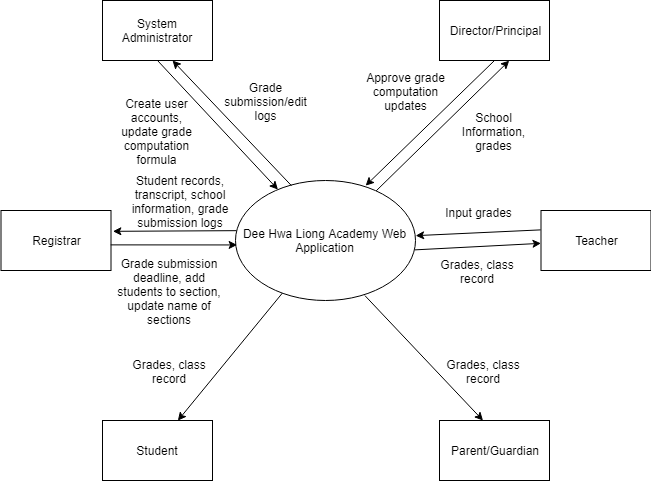
\includegraphics[height=10.5cm]{Context-Diagram.png}
  \vspace{2cm}
  \caption{Context Diagram, DHLA Grade Management System}
  \label{fig:cd}
\end{figure}

\newpage

\subsection{Data Flow Diagram}
\vspace{2cm}
\begin{figure}[H]
  \centering
  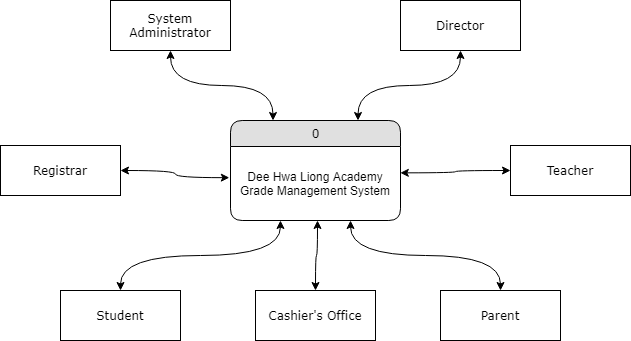
\includegraphics[height=7.5cm]{Data-Flow-Diagram-1.png}
  \vspace{2cm}
  \caption{Top Level Data Flow Diagram, DHLA Grade Management System}
  \label{fig:tldfd}
\end{figure}
\vspace{2cm}
\begin{figure}[H]
  \centering
  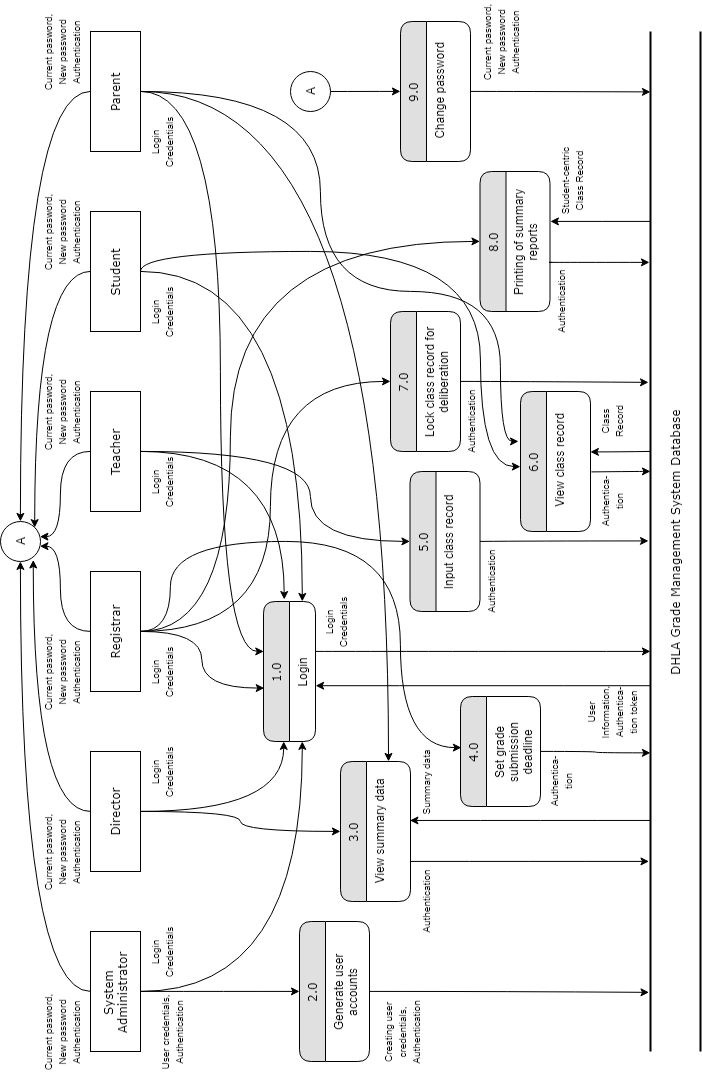
\includegraphics[height=20.5cm]{Data-Flow-Diagram-2.png}
  \vspace{2cm}
  \caption{Level 1 Data Flow Diagram, DHLA Grade Management System}
  \label{fig:l1dfd}
\end{figure}
\vspace{2cm}
\begin{figure}[H]
  \centering
  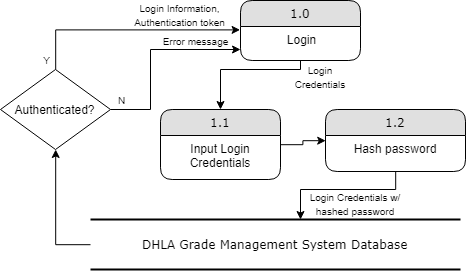
\includegraphics[height=5.5cm]{Subexplotion-1.png}
  \vspace{2cm}
  \caption{Level 2 Data Flow Diagram for Process 1.0, DHLA Grade Management System}
  \label{fig:l2dfd}
\end{figure}
\vspace{2cm}
\begin{figure}[H]
  \centering
  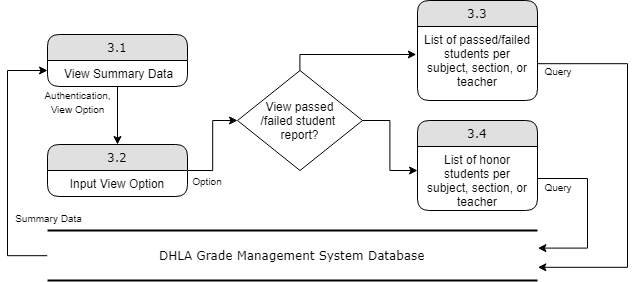
\includegraphics[height=5.5cm]{Subexplotion-3.png}
  \vspace{2cm}
  \caption{Level 2 Data Flow Diagram for Process 3.0, DHLA Grade Management System}
  \label{fig:l2dfd3}
\end{figure}
\vspace{2cm}
\begin{figure}[H]
  \centering
  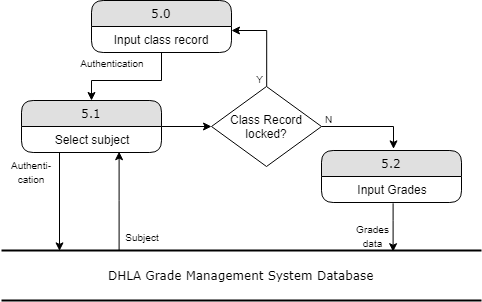
\includegraphics[height=6.5cm]{Subexplotion-5.png}
  \vspace{2cm}
  \caption{Level 2 Data Flow Diagram for Process 5.0, DHLA Grade Management System}
  \label{fig:l2dfd5}
\end{figure}
\vspace{2cm}

\subsection{Activity Diagrams}

All accounts will have a login and logout function. Each user account can also change the account's password. The password change is done within the system. No external links will be provided for password change. Profiles for each account will be available and can be updated.

The system administrator is the one managing the system.

The system administrator can create accounts for the other users such as director, registrar, teachers, and students. All account creation will not have any creation requests.

The administrator and registrar have an access to the activity logs of the class record. The activity log records every information changes that occur to class records in the system. It includes adding, updating, and deleting records. This activity log cannot be edited nor deleted, it is only readable. Both administrator and registrar can also search the log using date, time, teacher's name, section, school year, and grade level.

Activation and deactivation of accounts is also a functionality of the administrator. An account can be deactivated/deleted if the user is no long affiliated with the school.

The director can view grades of each subject and the condensed grades. Viewing of summary reports is also possible.

Summary reports will get all the information needed from the database of the system.

The school registrar is in charge of keeping student records.

The school registrar will be able to set the deadline for submission of grades. Different deadlines may be set for different teachers due to their workload differences. Deadline alerts will be automatically sent, by the system, during 5 days and 3 days before the deadline and during the deadline day.

Since a school registrar keeps student records, they can view record from past school years and produce unofficial TORs. Viewing of summary reports will also be possible. Summary reports may be requested by the principal, director, and/or the DepEd and PEAC.

School registrars can update the student list of each section by adding or removing students from the class list. They can also update the section name and view the submitted grade of teachers.

Another activity log will be present under this user, which is the submission logs of teachers. This will be used to check the teachers who failed to comply with the deadline set by the registrar.

A school will never be a school without its teachers. In this system, there are two types of teachers: teacher-only and teacher/advisers.

Both types can input and update the grades of students. Their class records will be automatically be available after they input the class and subjects they are handling in their profiles.

Both teacher-only and advisers can also submit the grades through the application to create the condensed grades sheet. Before submitting the grades, the teacher must be sure that there are no errors with the record. A save function will be available to save changes made in the class record.

The difference between teacher-only and teacher/adviser, teacher/adviser can view the condensed grades of their advisees from the profiles. In addition, teacher/adviser can view his/her advisees' report carrds after the condensed grades have been finalized.

Finally, the student, this user can only do simple things such as view grades from his/her past grade levels to present.

\vspace{2cm}
\begin{figure}[H]
  \centering
  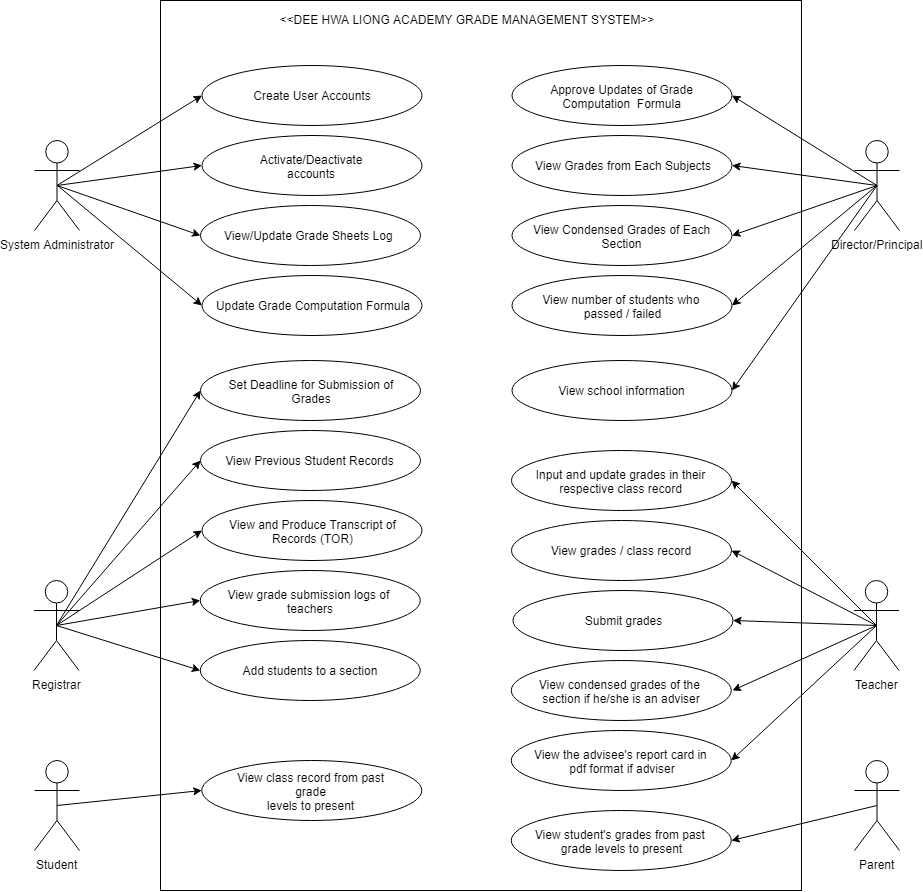
\includegraphics[height=14.5cm]{Activity-Diagram-1.png}
  \vspace{2cm}
  \caption{Use Case Diagram, DHLA Grade Management System}
  \label{fig:l2dfd5}
\end{figure}

\newpage
\subsection{Database Design}

\subsubsection{Entity Relationship Diagram (ERD)}

Figure~\ref{fig:erdua} shows the relationship among the user account, student, parent guardian, teacher, and nonacademic tables. The user account table contains the login credentials and basic information such as first name, last name, middle name, etc. of the user. System administrator, registrar, and principal/director fall under the nonacademic table.

Figure~\ref{fig:erdan} shows the relationship among student, and account notice. Account notice table is responsible for storing the message of cashier clerk in case a student account is restricted. It contains the studentID of a restricted student account.

Figure~\ref{fig:erdsy} shows the relationship among school year, student section, student final grade, attendance log, student grades, teacher section and subject section table. School year table contains the all the school year created in the system. schoolYear field indicates the school year name, isActive if the school year is currently active, and the current quarter.

Figure~\ref{fig:erds} shows the relationship among section, subject section, student section and teacher section. Section contains the basic information of a section such as sectionName, gradeLevel, and archived.

Figure~\ref{fig:erdts} shows the relationship among teacher section, school year, section, and teacher. Teacher section table contains all advisers in a specific school year. It also contains the teacherID, sectionID, and the schoolYearID.

Figure~\ref{fig:erdstudsect} shows the relationship among student section, student final grade, school year, student, student grades, subject section student, and section. Student section table contains the all students enrolled in a section for a given school year.

Figure~\ref{fig:erdss} shows the relationship among subject section, subject, teacher, section, subject section student, and school year. Subject section contains all subject loads of a teacher. It also contains basic information such as subjectID, sectionID, teacherID, schoolYearID, and classRecordID.

Figure~\ref{fig:erdcr} shows the relationship among the class record, component, grade, teacher, section, grade level, and subject. The class record table contains the collection of grades of students in a section. The component table shows the type of activity being recorded in the class record. The grade table contains an individual grade of the student, and other important information such as date, category, and entry number. The section table shows the section name of the class record. The subject table contains the subject code and the subject name of the class record.

Figure~\ref{fig:erdcrs} shows the relationship among the class record status and the class record. Class Record Status contains the current state of a class record indicated as follows: 'L' if the class record is locked, 'E' if the class record is for encoding, 'D" if the class record is under deliberation process, and 'F' if the class record is posted.

Figure~\ref{fig:erdg} shows the relationship among the grade, student, category, and class record. The grade table contains an individual grade of the student, and other important information such as date, category, and entry number. The category table shows the type of activity being recorded in the class record. The class record table contains the collection of grades of students in a section.

Figure~\ref{fig:erdssg} shows the relationship among the student subject grades, subject section student, and the class record. Student Subject Grades table contains the grade of each student from quarter 1 to quarter 2 of a subject section. It also contains the classRecordID, and the subjectstudID

Figure~\ref{fig:erdsws} shows the relationship among student weighted score, subject section student, and class record. Student Weighted Score contains the weighted score of a student in a given subject per component (Formative Assessment, Written Works, Performance Task, Quarterly Examinations). It also contains the overall grade of the student in a subject based on the given transmutation (50\%, 55\%, 60\% ).

Figure~\ref{fig:erdsg} shows the relationship among student grades, student section, and school year. Student Grades table contains the overall grade of the student (average of all subjet grades) in a given quarter and schoolYearID.

Figure~\ref{fig:erdsfg} shows the relationship among student final grade, student section, and school year. Student Final Grade table contains the overall grade of the student (average of all quarter grades) in a given school year.

Figure~\ref{fig:erdal} shows the relationship among activity log, log details, and class record. Activity Log table contains the class record update information. Whenever a registrar modifies a class record during deliberation process, all changes will reflect in this table.

Figure~\ref{fig:erdc} shows the relationship among component, grade, subcomponent, and subject. Component table contains the component name, and its corresponding weight. 

Figure~\ref{fig:erdsc} shows the relationship among subcomponent, grade, component, and class record. Subcomponent table contains information such as classRecordID, name, componentID, and compWeight. A teacher can add multiple subcomponents in a class record. He/she can also provide the weights of each subcomponent. All subcomponents must accumulate to 100\% in each component.



\vspace{1cm}
\begin{figure}[H]
  \centering
  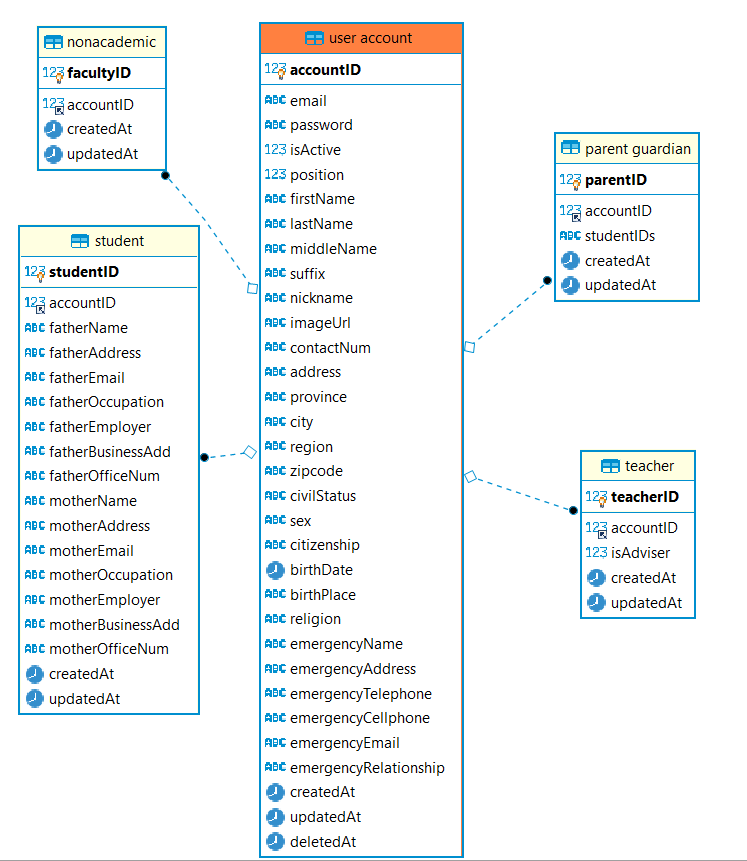
\includegraphics[height=16.5cm]{ERDUA.png}
  \vspace{1cm}
  \caption{Entity Relationship Diagram (ERD) (user account)}
  \label{fig:erdua}
\end{figure}
\vspace{1cm}
\begin{figure}[H]
  \centering
  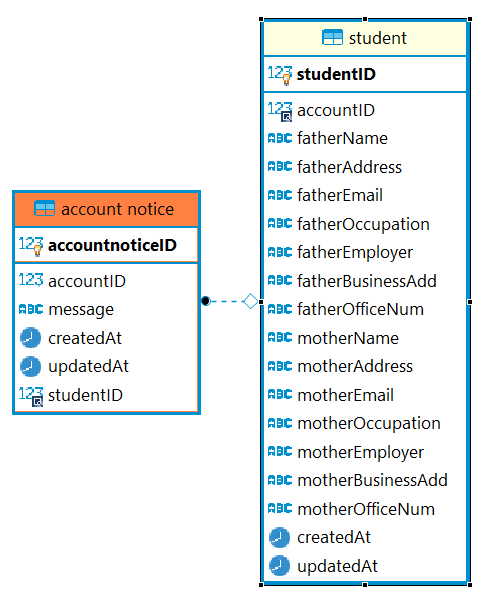
\includegraphics[height=10.5cm]{ERDAN.png}
  \vspace{1cm}
  \caption{Entity Relationship Diagram (ERD) (account notice)}
  \label{fig:erdan}
\end{figure}
\vspace{1cm}
\begin{figure}[H]
  \centering
  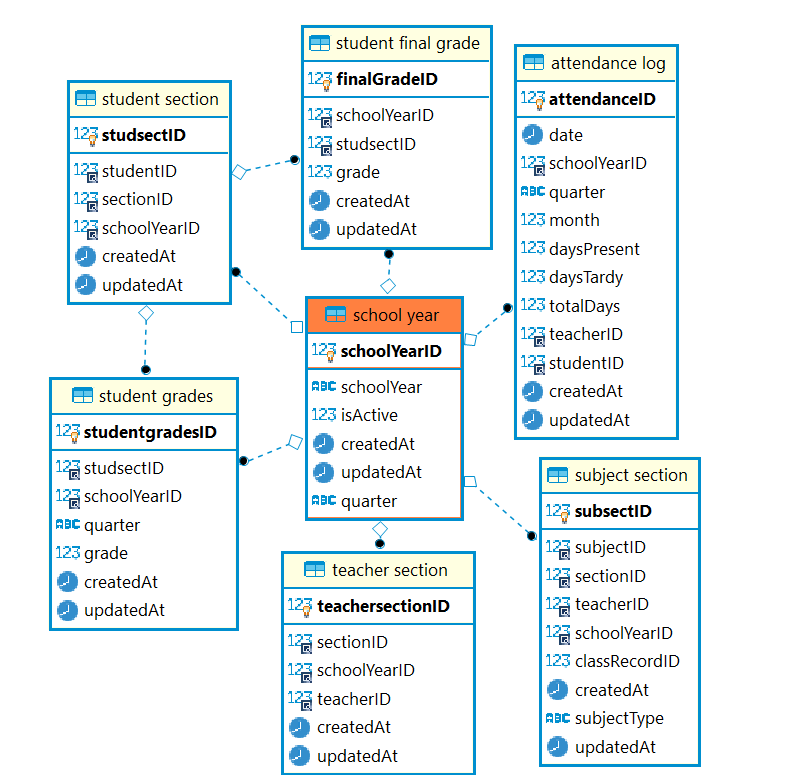
\includegraphics[height=13.5cm]{ERDSY.png}
  \vspace{1cm}
  \caption{Entity Relationship Diagram (ERD) (school year)}
  \label{fig:erdsy}
\end{figure}
\vspace{1cm}
\begin{figure}[H]
  \centering
  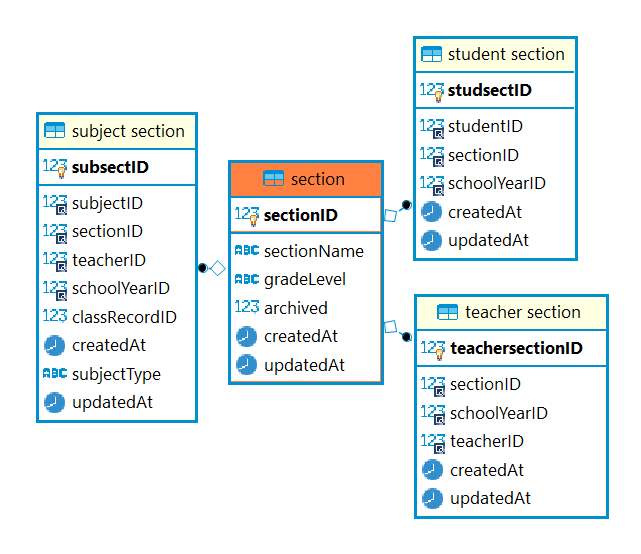
\includegraphics[height=8.5cm]{ERDS.png}
  \vspace{1cm}
  \caption{Entity Relationship Diagram (ERD) (section)}
  \label{fig:erds}
\end{figure}
\vspace{1cm}
\begin{figure}[H]
  \centering
  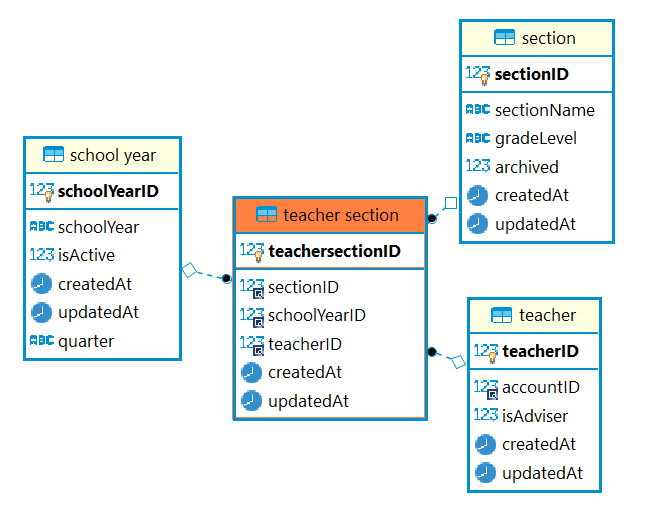
\includegraphics[height=8.5cm]{ERDTS.png}
  \vspace{1cm}
  \caption{Entity Relationship Diagram (ERD) (teacher section)}
  \label{fig:erdts}
\end{figure}
\vspace{1cm}
\begin{figure}[H]
  \centering
  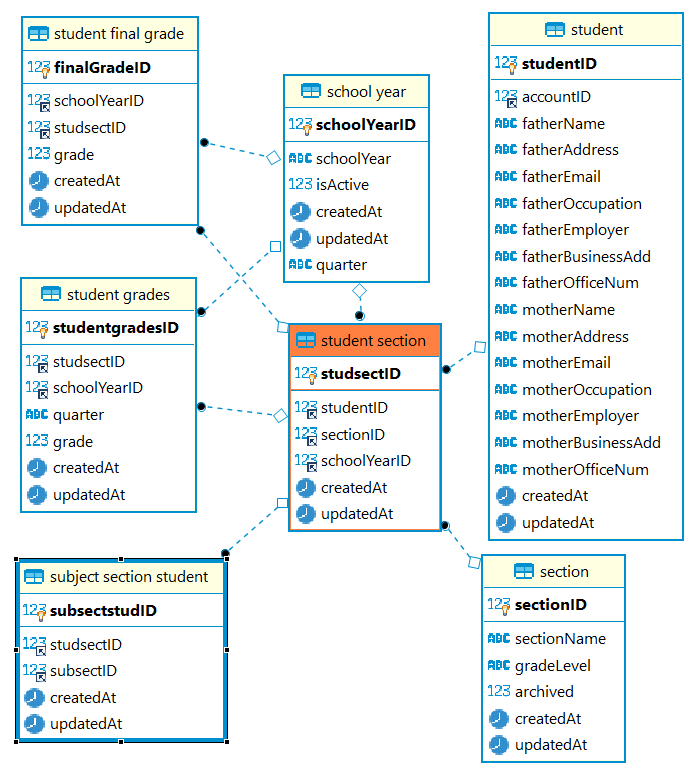
\includegraphics[height=13.5cm]{ERDSTUDSECT.png}
  \vspace{1cm}
  \caption{Entity Relationship Diagram (ERD) (student section)}
  \label{fig:erdstudsect}
\end{figure}
\begin{figure}[H]
    \centering
    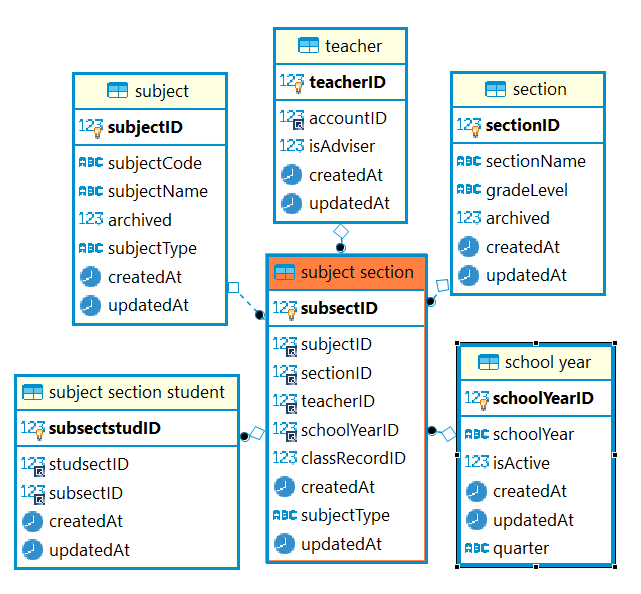
\includegraphics[height=10.5cm]{ERDSS.png}
    \vspace{1cm}
    \caption{Entity Relationship Diagram (ERD) (subject section)}
    \label{fig:erdss}
  \end{figure}
\vspace{1cm}
\begin{figure}[H]
  \centering
  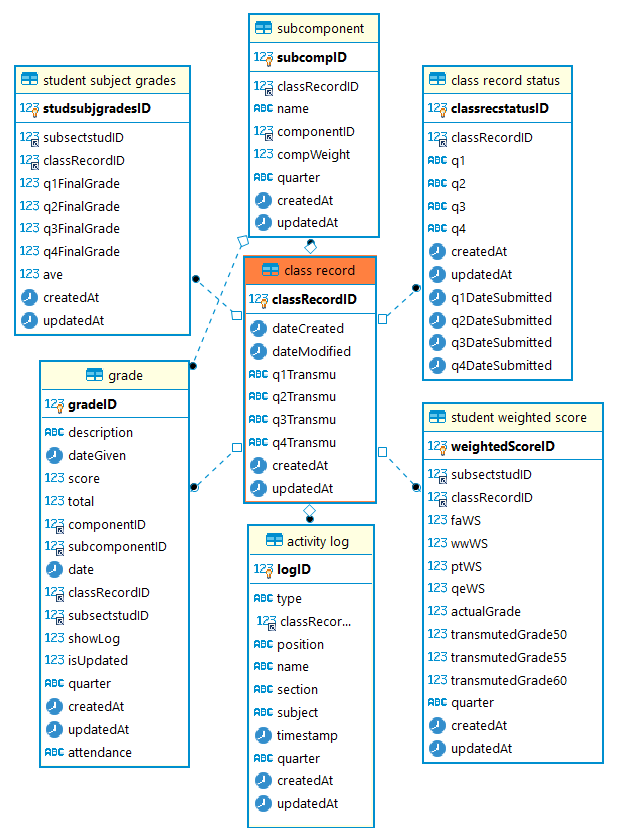
\includegraphics[height=16.5cm]{ERDCR.png}
  \vspace{1cm}
  \caption{Entity Relationship Diagram (ERD) (class record)}
  \label{fig:erdcr}
\end{figure}
\vspace{1cm}
\begin{figure}[H]
  \centering
  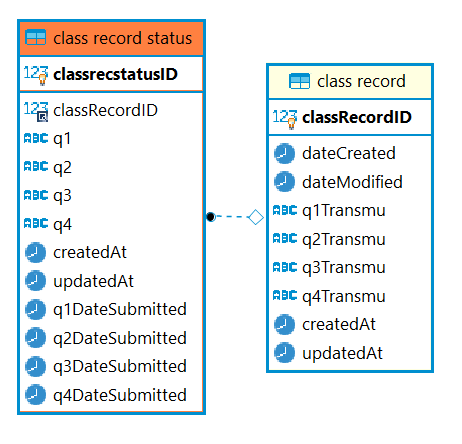
\includegraphics[height=8.5cm]{ERDCRS.png}
  \vspace{1cm}
  \caption{Entity Relationship Diagram (ERD) (class record status)}
  \label{fig:erdcrs}
\end{figure}
\vspace{1cm}
\begin{figure}[H]
  \centering
  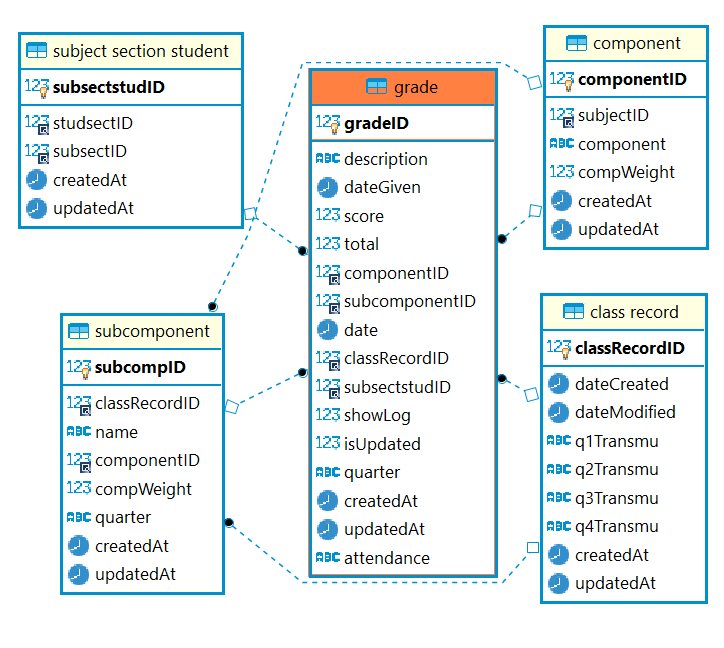
\includegraphics[height=12.5cm]{ERDG.png}
  \vspace{1cm}
  \caption{Entity Relationship Diagram (ERD) (grade)}
  \label{fig:erdg}
\end{figure}
\vspace{1cm}
\begin{figure}[H]
  \centering
  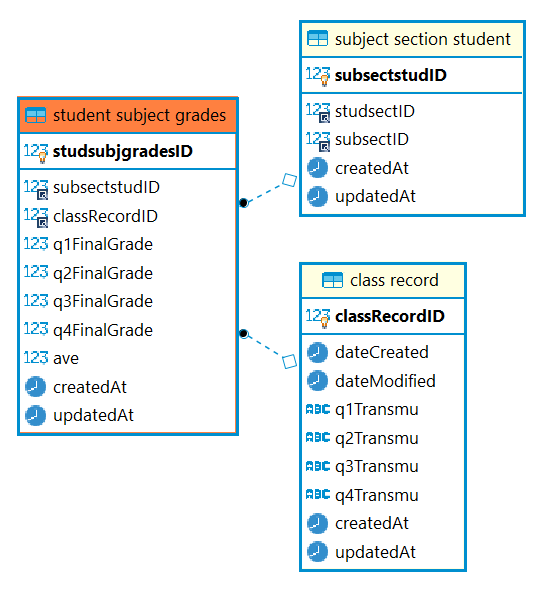
\includegraphics[height=9.5cm]{ERDSSG.png}
  \vspace{1cm}
  \caption{Entity Relationship Diagram (ERD) (student subject grades)}
  \label{fig:erdssg}
\end{figure}
\vspace{1cm}
\begin{figure}[H]
  \centering
  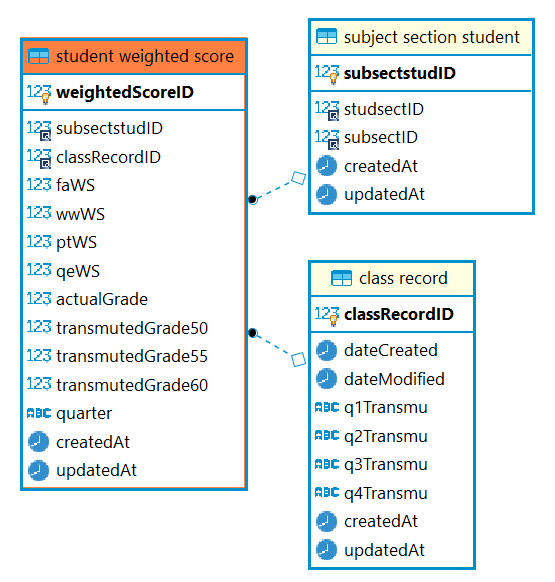
\includegraphics[height=9.5cm]{ERDSWS.png}
  \vspace{1cm}
  \caption{Entity Relationship Diagram (ERD) (student weighted score)}
  \label{fig:erdsws}
\end{figure}
\vspace{1cm}
\begin{figure}[H]
  \centering
  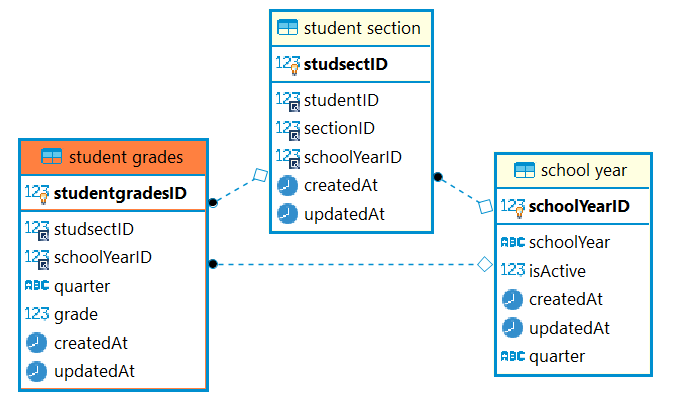
\includegraphics[height=7.5cm]{ERDSG.png}
  \vspace{1cm}
  \caption{Entity Relationship Diagram (ERD) (student grades)}
  \label{fig:erdsg}
\end{figure}
\vspace{1cm}
\begin{figure}[H]
  \centering
  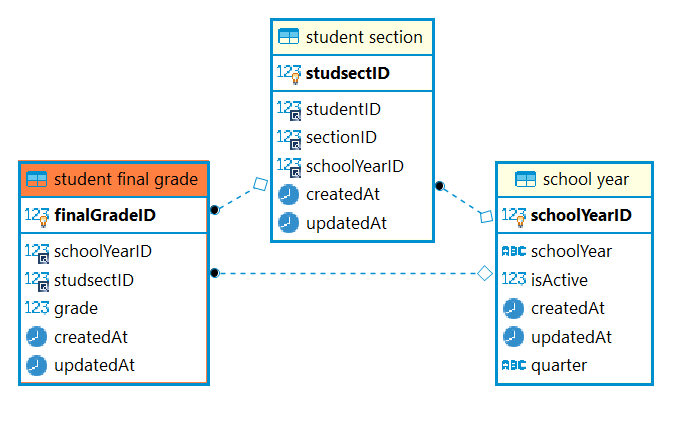
\includegraphics[height=7.5cm]{ERDSFG.png}
  \vspace{1cm}
  \caption{Entity Relationship Diagram (ERD) (student final grade)}
  \label{fig:erdsfg}
\end{figure}
\vspace{1cm}
\begin{figure}[H]
  \centering
  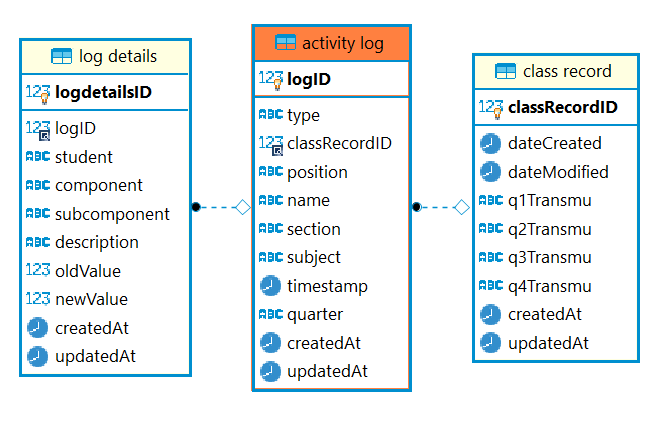
\includegraphics[height=7.5cm]{ERDAL.png}
  \vspace{1cm}
  \caption{Entity Relationship Diagram (ERD) (activity log)}
  \label{fig:erdal}
\end{figure}
\vspace{1cm}
\begin{figure}[H]
  \centering
  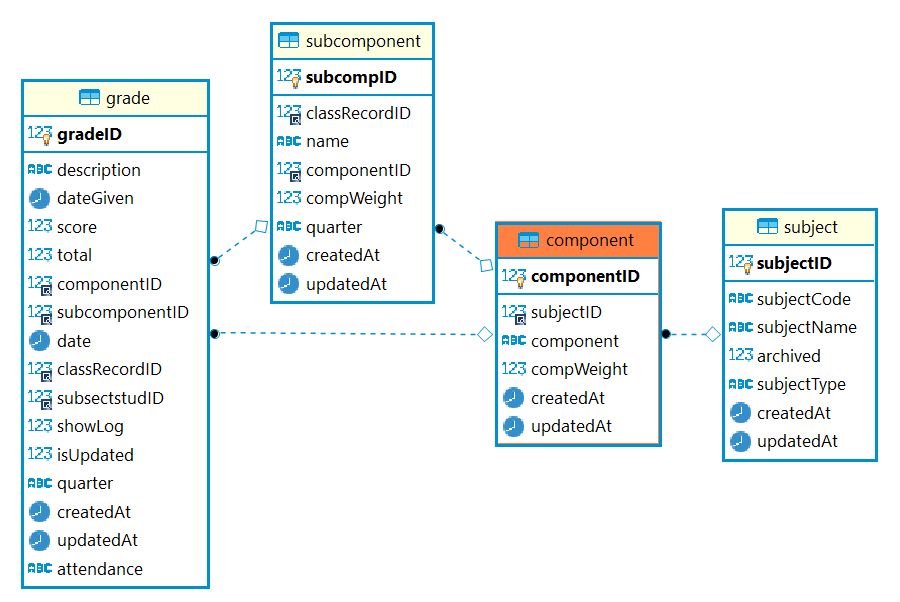
\includegraphics[height=8.5cm]{ERDC.png}
  \vspace{1cm}
  \caption{Entity Relationship Diagram (ERD) (component)}
  \label{fig:erdc}
\end{figure}
\vspace{1cm}
\begin{figure}[H]
  \centering
  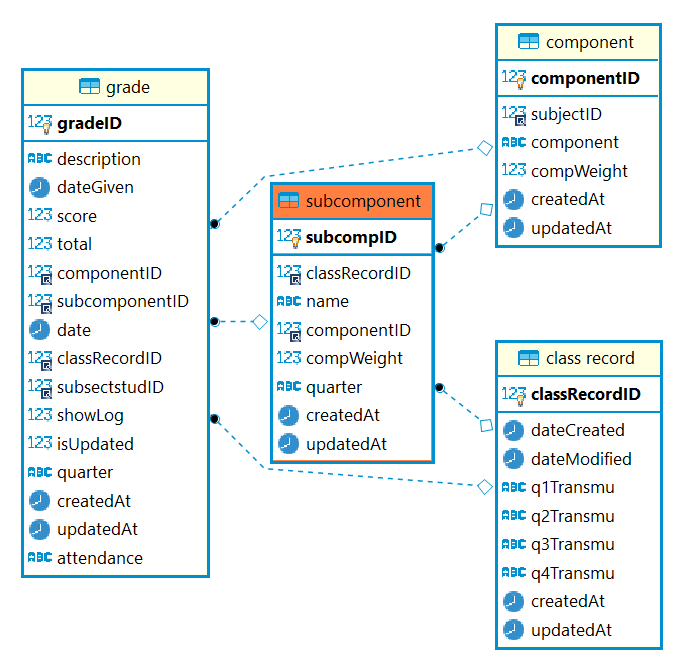
\includegraphics[height=10.0cm]{ERDSC.png}
  \vspace{1cm}
  \caption{Entity Relationship Diagram (ERD) (subcomponent)}
  \label{fig:erdsc}
\end{figure}

\newpage

\subsection{Data Dictionary}

Shown below are the database tables. Primary keys are in bold format.

\subsubsection{Account Notice}

This table is used for storing personalized messages for restricted students made by the cashier.

\vspace{1cm} \begin{longtable}{ |p{2.5cm}|p{4.5cm}|p{2.5cm}|p{3cm}| } \hline \multicolumn{4}{|c|}{\textbf{account notice}}\\ \hline \textbf{FIELD}&\textbf{TYPE}&\textbf{KEY TYPE}&\textbf{DESCRIPTION}\\ \hline \textbf{accountnoti- ceID} & \textbf{INT(11), AUTO INCREMENT} & \textbf{PRIMARY} & \textbf{Unique identifier of an account notice}\\ \hline accountID & INT(11) & FOREIGN & Unique identifier of a user account \\ \hline message & VARCHAR(100) & & Message of the cashier to the student \\ \hline studentID & INT(11) & FOREIGN & Unique identifier of the student \\ \hline \caption{Data dictionary for \textbf{account notice} table} \end{longtable} 

\subsubsection{Activity Log}

This table is used for storing all informations regarding changes in class records. Changes are usually made by the registrar.

\vspace{1cm} \begin{longtable}{ |p{2.5cm}|p{4.5cm}|p{2.5cm}|p{3cm}| } \hline \multicolumn{4}{|c|}{\textbf{activity log}}\\ \hline \textbf{FIELD}&\textbf{TYPE}&\textbf{KEY TYPE}&\textbf{DESCRIPTION}\\ \hline \textbf{logID} & \textbf{INT(11), AUTO INCREMENT} & \textbf{PRIMARY} & \textbf{Unique identifier of an activity log}\\ \hline type & ENUM & & Type of the activity log \\ \hline classRecordID & INT(11) & FOREIGN & Unique identifier of a class record \\ \hline position & VARCHAR(255) & & The position of the user who made the changes \\ \hline name & VARCHAR(255) & & Name of the user who made the changes \\ \hline section & VARCHAR(255) & & Section of the class record \\ \hline subject & VARCHAR(255) & & Subject of the class record \\ \hline timestamp & DATETIME & & Date modified \\ \hline quarter & VARCHAR & & Activity log current quarter \\ \hline \caption{Data dictionary for \textbf{activity log} table} \end{longtable} 

\subsubsection{Class Record}

This table is used as a header of grade table. It contains information such as transmutation of each quarter, date created, and date modified.

\vspace{1cm} \begin{longtable}{ |p{2.5cm}|p{4.5cm}|p{2.5cm}|p{3cm}| } \hline \multicolumn{4}{|c|}{\textbf{class record}}\\ \hline \textbf{FIELD}&\textbf{TYPE}&\textbf{KEY TYPE}&\textbf{DESCRIPTION}\\ \hline \textbf{classRecordID} & \textbf{INT(11), AUTO INCREMENT} & \textbf{PRIMARY} & \textbf{Unique identifier of a class record}\\ \hline dateCreated & DATETIME & & Date created \\ \hline dateModified & DATETIME & & Date modified \\ \hline q1Transmu & ENUM & & Transmutation used for quarter 1 \\ \hline q2Transmu & ENUM & & Transmutation used for quarter 2 \\ \hline q3Transmu & ENUM & & Transmutation used for quarter 3 \\ \hline q4Transmu & ENUM & & Transmutation used for quarter 4 \\ \hline \caption{Data dictionary for \textbf{class record} table} \end{longtable} 

\subsubsection{Class Record Status}

This table is used to determine the current status of a class record.

\vspace{1cm} \begin{longtable}{ |p{2.5cm}|p{4.5cm}|p{2.5cm}|p{3cm}| } \hline \multicolumn{4}{|c|}{\textbf{class record status}}\\ \hline \textbf{FIELD}&\textbf{TYPE}&\textbf{KEY TYPE}&\textbf{DESCRIPTION}\\ \hline \textbf{classrecstatu- sID} & \textbf{INT(11), AUTO INCREMENT} & \textbf{PRIMARY} & \textbf{Unique identifier of a class record status}\\ \hline classRecordID & INT(11) & FOREIGN & Unique identifier of a class record ID \\ \hline q1 & ENUM & & Status of the first quarter \\ \hline q2 & ENUM & & Status of the second quarter \\ \hline q3 & ENUM & & Status of the third quarter \\ \hline q4 & ENUM & & Status of the fourth quarter \\ \hline q1DateSubmi- tted & DATETIME & & Date submitted for quarter 1 \\ \hline q2DateSubmi- tted & DATETIME & & Date submitted for quarter 2 \\ \hline q3DateSubmi- tted & DATETIME & & Date submitted for quarter 3 \\ \hline q4DateSubmi- tted & DATETIME & & Date submitted for quarter 4 \\ \hline \caption{Data dictionary for \textbf{class record status} table} \end{longtable} 

\subsubsection{Component}

This look-up table is used to determine the weights of each component per subject.

\vspace{1cm} \begin{longtable}{ |p{2.5cm}|p{4.5cm}|p{2.5cm}|p{3cm}| } \hline \multicolumn{4}{|c|}{\textbf{component}}\\ \hline \textbf{FIELD}&\textbf{TYPE}&\textbf{KEY TYPE}&\textbf{DESCRIPTION}\\ \hline \textbf{componentID} & \textbf{INT(11), AUTO INCREMENT} & \textbf{PRIMARY} & \textbf{Unique identifier of a component}\\ \hline subjectID & INT(11) & FOREIGN & Unique identifier of a subject \\ \hline component & ENUM & & Indicates the component name \\ \hline compWeight & FLOAT & & Indicates the weight of the component \\ \hline \caption{Data dictionary for \textbf{component} table} \end{longtable} 

\subsubsection{Grade}

This table is used to store student grades per subcomponent. It contains information such as description, date given, score, and total.

\vspace{1cm} \begin{longtable}{ |p{2.5cm}|p{4.5cm}|p{2.5cm}|p{3cm}| } \hline \multicolumn{4}{|c|}{\textbf{grade}}\\ \hline \textbf{FIELD}&\textbf{TYPE}&\textbf{KEY TYPE}&\textbf{DESCRIPTION}\\ \hline \textbf{gradeID} & \textbf{INT(11), AUTO INCREMENT} & \textbf{PRIMARY} & \textbf{Unique identifier of a grade}\\ \hline description & VARCHAR(100) & & Description of the grade item \\ \hline & & & \\ \hline dateGiven & DATETIME & & Date on which the item was given \\ \hline score & FLOAT & & Score of the student \\ \hline total & FLOAT & & Total number of items \\ \hline componentID & INT(11) & FOREIGN & Unique identifier of a component \\ \hline subcompone- ntID & INT(11) & FOREIGN & Unique identifier of a subcomponent \\ \hline date & DATETIME & & Date on which the grades were added \\ \hline classRecordID & INT(11) & FOREIGN & Unique identifier of a class record \\ \hline subsectstudID & INT(11) & & Unique identifier of a student \\ \hline quarter & ENUM & & Current quarter \\ \hline \caption{Data dictionary for \textbf{grade} table} \end{longtable} 

\subsubsection{Log Details}

This table is used to provide more information regarding activity log table.

\vspace{1cm} \begin{longtable}{ |p{2.5cm}|p{4.5cm}|p{2.5cm}|p{3cm}| } \hline \multicolumn{4}{|c|}{\textbf{log details}}\\ \hline \textbf{FIELD}&\textbf{TYPE}&\textbf{KEY TYPE}&\textbf{DESCRIPTION}\\ \hline \textbf{logdetailsID} & \textbf{INT(11), AUTO INCREMENT} & \textbf{PRIMARY} & \textbf{Unique identifier of a log detail}\\ \hline logID & INT(11) & FOREIGN & Unique identifier of an activity log \\ \hline student & VARCHAR(255) & & Name of the student \\ \hline component & VARCHAR(255) & & Name of the component \\ \hline subcomponent & VARCHAR(255) & & Name of the subcomponent \\ \hline description & VARCHAR(255) & & A short description of the log detail \\ \hline oldValue & FLOAT & & Old value \\ \hline newValue & FLOAT & & New value \\ \hline \caption{Data dictionary for \textbf{log details} table} \end{longtable} 

\subsubsection{Nonacademic}

This table is used to store basic information of nonacademic accounts.

\vspace{1cm} \begin{longtable}{ |p{2.5cm}|p{4.5cm}|p{2.5cm}|p{3cm}| } \hline \multicolumn{4}{|c|}{\textbf{nonacademic}}\\ \hline \textbf{FIELD}&\textbf{TYPE}&\textbf{KEY TYPE}&\textbf{DESCRIPTION}\\ \hline \textbf{facultyID} & \textbf{INT(11), AUTO INCREMENT} & \textbf{PRIMARY} & \textbf{Unique identifier of a nonacademic user}\\ \hline accountID & INT(11) & FOREIGN & Unique identifier of a user account \\ \hline \caption{Data dictionary for \textbf{nonacademic} table} \end{longtable} 

\subsubsection{Parent Guardian}

This table is used to store basic information of parent guardian accounts.

\vspace{1cm} \begin{longtable}{ |p{2.5cm}|p{4.5cm}|p{2.5cm}|p{3cm}| } \hline \multicolumn{4}{|c|}{\textbf{parent guardian}}\\ \hline \textbf{FIELD}&\textbf{TYPE}&\textbf{KEY TYPE}&\textbf{DESCRIPTION}\\ \hline \textbf{parentID} & \textbf{INT(11), AUTO INCREMENT} & \textbf{PRIMARY} & \textbf{Unique identifier of a parent account}\\ \hline accountID & INT(11) & FOREIGN & Unique identifier of a user account \\ \hline studentIDs & VARCHAR(1000) & & Contains a stringified array of all students of the parent \\ \hline \caption{Data dictionary for \textbf{parent guardian} table} \end{longtable} 

\subsubsection{School Year}

This table is used to store school year information.

\vspace{1cm} \begin{longtable}{ |p{2.5cm}|p{4.5cm}|p{2.5cm}|p{3cm}| } \hline \multicolumn{4}{|c|}{\textbf{school year}}\\ \hline \textbf{FIELD}&\textbf{TYPE}&\textbf{KEY TYPE}&\textbf{DESCRIPTION}\\ \hline \textbf{schoolYearID} & \textbf{INT(11), AUTO INCREMENT} & \textbf{PRIMARY} & \textbf{Unique identifier of a school year}\\ \hline schoolYear & VARCHAR(9) & & School year name \\ \hline isActive & TINYINT & & 1 if the school year is currently active. Otherwise, 0 \\ \hline quarter & ENUM & & Current active quarter \\ \hline \caption{Data dictionary for \textbf{school year} table} \end{longtable} 

\subsubsection{Section}

This table is used to store all active and inactive sections for all school years.

\vspace{1cm} \begin{longtable}{ |p{2.5cm}|p{4.5cm}|p{2.5cm}|p{3cm}| } \hline \multicolumn{4}{|c|}{\textbf{section}}\\ \hline \textbf{FIELD}&\textbf{TYPE}&\textbf{KEY TYPE}&\textbf{DESCRIPTION}\\ \hline \textbf{sectionID} & \textbf{INT(11), AUTO INCREMENT} & \textbf{PRIMARY} & \textbf{Unique identifier of a section}\\ \hline sectionName & VARCHAR(100) & & Name of the section \\ \hline gradeLevel & ENUM & & Grade level of the section \\ \hline archived & TINYINT & & 1 if the section is archived. Otherwise, 0 \\ \hline \caption{Data dictionary for \textbf{section} table} \end{longtable} 

\subsubsection{Student}

This table is used to store basic information of students.

\vspace{1cm} \begin{longtable}{ |p{2.5cm}|p{4.5cm}|p{2.5cm}|p{3cm}| } \hline \multicolumn{4}{|c|}{\textbf{student}}\\ \hline \textbf{FIELD}&\textbf{TYPE}&\textbf{KEY TYPE}&\textbf{DESCRIPTION}\\ \hline \textbf{studentID} & \textbf{INT(11), AUTO INCREMENT} & \textbf{PRIMARY} & \textbf{Unique identifier of the student}\\ \hline accountID & INT(11) & FOREIGN & Unique identifier of a user account \\ \hline fatherName & VARCHAR(3) & & Name of the father \\ \hline fatherAddress & VARCHAR(30) & & Address of the father \\ \hline fatherEmail & VARCHAR(30) & & Email of the father \\ \hline fatherOccupa- tion & VARCHAR(30) & & Occupation of the father \\ \hline fatherEmployer & VARCHAR(30) & & Employer of the father \\ \hline fatherBusine- ssAdd & VARCHAR(30) & & Business address of the father \\ \hline fatherOffice- Num & VARCHAR(30) & & Office number of the father \\ \hline motherName & VARCHAR(30) & & Name of the mother \\ \hline motherAddress & VARCHAR(30) & & Address of the mother \\ \hline motherEmail & VARCHAR(30) & & Email of the mother \\ \hline motherOccu- pation & VARCHAR(30) & & Occupation of the mother \\ \hline motherEmplo- yer & VARCHAR(30) & & Employer of the mother \\ \hline motherBusi- nessAdd & VARCHAR(30) & & Business address of the mother \\ \hline motherOffice- Num & VARCHAR(30) & & Office number of the mother \\ \hline \caption{Data dictionary for \textbf{student} table} \end{longtable} 

\subsubsection{Student Final Grade}

This table is used to store the overall grade of students in a given school year.

\vspace{1cm} \begin{longtable}{ |p{2.5cm}|p{4.5cm}|p{2.5cm}|p{3cm}| } \hline \multicolumn{4}{|c|}{\textbf{student final grade}}\\ \hline \textbf{FIELD}&\textbf{TYPE}&\textbf{KEY TYPE}&\textbf{DESCRIPTION}\\ \hline \textbf{finalGradeID} & \textbf{INT(11), AUTO INCREMENT} & \textbf{PRIMARY} & \textbf{Unique identifier of a student final grade}\\ \hline schoolYearID & INT(11) & FOREIGN & Unique identifier of a school year \\ \hline studsectID & INT(11) & FOREIGN & Unique identifier of a student section \\ \hline grade & FLOAT & & Grade of the student \\ \hline \caption{Data dictionary for \textbf{student final grade} table} \end{longtable} 

\subsubsection{Student Grades}

This table is used to store the overall grade of students per quarter in a given school year.

\vspace{1cm} \begin{longtable}{ |p{2.5cm}|p{4.5cm}|p{2.5cm}|p{3cm}| } \hline \multicolumn{4}{|c|}{\textbf{student grade}}\\ \hline \textbf{FIELD}&\textbf{TYPE}&\textbf{KEY TYPE}&\textbf{DESCRIPTION}\\ \hline \textbf{studentgra- desID} & \textbf{INT(11), AUTO INCREMENT} & \textbf{PRIMARY} & \textbf{Unique identifier of a student grade}\\ \hline studsectID & INT(11) & FOREIGN & Unique identifier of a student section \\ \hline schoolYearID & INT(11) & FOREIGN & Unique identifier of a school year \\ \hline quarter & ENUM & & Current active quarter \\ \hline grade & FLOAT & & Grade of the student \\ \hline \caption{Data dictionary for \textbf{student grade} table} \end{longtable} 

\subsubsection{Student Section}

This table is used to store all enrolled students (enrolled in a section) in a given school year.

\vspace{1cm} \begin{longtable}{ |p{2.5cm}|p{4.5cm}|p{2.5cm}|p{3cm}| } \hline \multicolumn{4}{|c|}{\textbf{student section}}\\ \hline \textbf{FIELD}&\textbf{TYPE}&\textbf{KEY TYPE}&\textbf{DESCRIPTION}\\ \hline \textbf{studsectID} & \textbf{INT(11), AUTO INCREMENT} & \textbf{PRIMARY} & \textbf{Unique identifier of a student section}\\ \hline studentID & INT(11) & FOREIGN & Unique identifier of a student \\ \hline sectionID & INT(11) & FOREIGN & Unique identifier of a section \\ \hline schoolYearID & INT(11) & FOREIGN & Unique identifier of a school year \\ \hline \caption{Data dictionary for \textbf{student section} table} \end{longtable} 

\subsubsection{Student Subject Grades}

This table is used to store the overall grade of subjects per student in a given quarter.

\vspace{1cm} \begin{longtable}{ |p{2.5cm}|p{4.5cm}|p{2.5cm}|p{3cm}| } \hline \multicolumn{4}{|c|}{\textbf{student subject grades}}\\ \hline \textbf{FIELD}&\textbf{TYPE}&\textbf{KEY TYPE}&\textbf{DESCRIPTION}\\ \hline \textbf{studsubjgra- desID} & \textbf{INT(11), AUTO INCREMENT} & \textbf{PRIMARY} & \textbf{Unique identifier of a student subject grade}\\ \hline subsectstudID & INT(11) & FOREIGN & Unique identifier of a subject section student \\ \hline classRecordID & INT(11) & FOREIGN & Unique identifier of a class record \\ \hline q1FinalGrade & FLOAT & & Final grade of the student in quarter 1 \\ \hline q2FinalGrade & FLOAT & & Final grade of the student in quarter 2 \\ \hline q3FinalGrade & FLOAT & & Final grade of the student in quarter 3 \\ \hline q4FinalGrade & FLOAT & & Final grade of the student in quarter 4 \\ \hline ave & FLOAT & & Average of grades in all quarters \\ \hline \caption{Data dictionary for \textbf{student subject grades} table} \end{longtable} 

\subsubsection{Student Weighted Score}

This table is used to store the weighted scores of students for each components in a given class record.

\vspace{1cm} \begin{longtable}{ |p{2.5cm}|p{4.5cm}|p{2.5cm}|p{3cm}| } \hline \multicolumn{4}{|c|}{\textbf{student weighted score}}\\ \hline \textbf{FIELD}&\textbf{TYPE}&\textbf{KEY TYPE}&\textbf{DESCRIPTION}\\ \hline \textbf{weighted- ScoreID} & \textbf{INT(11), AUTO INCREMENT} & \textbf{PRIMARY} & \textbf{Unique identifier of a student weighted score}\\ \hline subsectstudID & INT(11) & FOREIGN & Unique identifier of a subject section student \\ \hline classRecordID & INT(11) & FOREIGN & Unique identifier of a class record \\ \hline faWS & FLOAT & & Weighted score for the formative assessment component \\ \hline wwWS & FLOAT & & Weighted score for the written works component \\ \hline ptWS & FLOAT & & Weighted score for the performance tasks component \\ \hline qeWS & FLOAT & & Weighted score for the quarterly exams component \\ \hline actualGrade & FLOAT & & Actual grade of the student \\ \hline transmuted- Grade50 & FLOAT & & Transmuted 50 grade of student \\ \hline transmuted- Grade55 & FLOAT & & Transmuted 55 grade of student \\ \hline transmuted- Grade60 & FLOAT & & Transmuted 60 grade of student \\ \hline quarter & ENUM & & Current active quarter \\ \hline \caption{Data dictionary for \textbf{student weighted score} table} \end{longtable} 

\subsubsection{Subcomponent}

This table is used to store the teacher defined subcomponents in a given component and class record.

\vspace{1cm} \begin{longtable}{ |p{2.5cm}|p{4.5cm}|p{2.5cm}|p{3cm}| } \hline \multicolumn{4}{|c|}{\textbf{subcomponent}}\\ \hline \textbf{FIELD}&\textbf{TYPE}&\textbf{KEY TYPE}&\textbf{DESCRIPTION}\\ \hline \textbf{subcompID} & \textbf{INT(11), AUTO INCREMENT} & \textbf{PRIMARY} & \textbf{Unique identifier of a subcomponent}\\ \hline classRecordID & INT(11) & FOREIGN & Unique identifier of a class record \\ \hline name & VARCHAR(50) & & Name of the subcomponent \\ \hline componentID & INT(11) & FOREIGN & Unique identifier of a componnet \\ \hline compWeight & FLOAT & & Weight of the subcomponent \\ \hline quarter & ENUM & & Current active quarter \\ \hline \caption{Data dictionary for \textbf{subcomponent} table} \end{longtable} 

\subsubsection{Subject}

This look-up table is used to store all subjects available for all grade levels.

\vspace{1cm} \begin{longtable}{ |p{2.5cm}|p{4.5cm}|p{2.5cm}|p{3cm}| } \hline \multicolumn{4}{|c|}{\textbf{subject}}\\ \hline \textbf{FIELD}&\textbf{TYPE}&\textbf{KEY TYPE}&\textbf{DESCRIPTION}\\ \hline \textbf{subjectID} & \textbf{INT(11), AUTO INCREMENT} & \textbf{PRIMARY} & \textbf{Unique identifier of a subject}\\ \hline subjectCode & VARCHAR(255) & & Subject code of the subject \\ \hline subjectName & VARCHAR(255) & & Subject name of the subject \\ \hline archived & TINYINT & & 1 if the subject is acrhived. Otherwise, 0 \\ \hline subjectType & ENUM & & Subject type of the subject \\ \hline \caption{Data dictionary for \textbf{subject} table} \end{longtable} 

\subsubsection{Subject Section}

This table is used to store all subject loads of all teachers in a given school year.

\vspace{1cm} \begin{longtable}{ |p{2.5cm}|p{4.5cm}|p{2.5cm}|p{3cm}| } \hline \multicolumn{4}{|c|}{\textbf{subject section}}\\ \hline \textbf{FIELD}&\textbf{TYPE}&\textbf{KEY TYPE}&\textbf{DESCRIPTION}\\ \hline \textbf{subsectID} & \textbf{INT(11), AUTO INCREMENT} & \textbf{PRIMARY} & \textbf{Unique identifier of a subject section}\\ \hline subjectID & INT(11) & FOREIGN & Unique identifier of a subject \\ \hline sectionID & INT(11) & FOREIGN & Unique identifier of a section \\ \hline teacherID & INT(11) & FOREIGN & Unique identifier of a teacher \\ \hline schoolYearID & INT(11) & FOREIGN & Unique identifier of a school year \\ \hline classRecordID & INT(11) & FOREIGN & Unique identifier of a class record \\ \hline subjectType & ENUM & & Subject type of the subject section \\ \hline \caption{Data dictionary for \textbf{subject section} table} \end{longtable} 

\subsubsection{Subject Section Student}

This table is used to store all students enrolled in a subject section

\vspace{1cm} \begin{longtable}{ |p{2.5cm}|p{4.5cm}|p{2.5cm}|p{3cm}| } \hline \multicolumn{4}{|c|}{\textbf{subject section student}}\\ \hline \textbf{FIELD}&\textbf{TYPE}&\textbf{KEY TYPE}&\textbf{DESCRIPTION}\\ \hline \textbf{subsectstudID} & \textbf{INT(11), AUTO INCREMENT} & \textbf{PRIMARY} & \textbf{Unique identifier of a subject section student}\\ \hline studsectID & INT(11) & FOREIGN & Unique identifier of a student section \\ \hline subsectID & INT(11) & FOREIGN & Unique identifier of a subject section \\ \hline \caption{Data dictionary for \textbf{subject section student} table} \end{longtable} 

\subsubsection{Submission Deadline}

This table is used to store all deadlines set for all teachers.

\vspace{1cm} \begin{longtable}{ |p{2.5cm}|p{4.5cm}|p{2.5cm}|p{3cm}| } \hline \multicolumn{4}{|c|}{\textbf{submission deadline}}\\ \hline \textbf{FIELD}&\textbf{TYPE}&\textbf{KEY TYPE}&\textbf{DESCRIPTION}\\ \hline \textbf{deadlineID} & \textbf{INT(11), AUTO INCREMENT} & \textbf{PRIMARY} & \textbf{Unique identifier of a submission deadline}\\ \hline teacherID & INT(11) & FOREIGN & Unique identifier of a teacher \\ \hline dateSet & DATETIME & & Date set \\ \hline deadline & DATETIME & & Deadline of the teacher \\ \hline isActive & TINYINT & & 1 if the deadline is active. Otherwise, 0 \\ \hline \caption{Data dictionary for \textbf{submission deadline} table} \end{longtable}

\subsubsection{Teacher}

This table is used to store basic information of a teacher.

\vspace{1cm} \begin{longtable}{ |p{2.5cm}|p{4.5cm}|p{2.5cm}|p{3cm}| } \hline \multicolumn{4}{|c|}{\textbf{teacher}}\\ \hline \textbf{FIELD}&\textbf{TYPE}&\textbf{KEY TYPE}&\textbf{DESCRIPTION}\\ \hline \textbf{teacherID} & \textbf{INT(11), AUTO INCREMENT} & \textbf{PRIMARY} & \textbf{Unique identifier of a teacher}\\ \hline accountID & INT(11) & FOREIGN & Unique identifier of a user account \\ \hline \caption{Data dictionary for \textbf{teacher} table} \end{longtable}

\subsubsection{Teacher Section}

This table is used to store all advisers in a given school year.

\vspace{1cm} \begin{longtable}{ |p{2.5cm}|p{4.5cm}|p{2.5cm}|p{3cm}| } \hline \multicolumn{4}{|c|}{\textbf{teacher section}}\\ \hline \textbf{FIELD}&\textbf{TYPE}&\textbf{KEY TYPE}&\textbf{DESCRIPTION}\\ \hline \textbf{teachersec- tionID} & \textbf{INT(11), AUTO INCREMENT} & \textbf{PRIMARY} & \textbf{Unique identifier of a teacher section}\\ \hline sectionID & INT(11) & FOREIGN & Section assign for the teacher \\ \hline schoolYearID & INT(11) & FOREIGN & Unique identifier of a school year \\ \hline teacherID & INT(11) & FOREIGN & Unique identifier of a teacher \\ \hline \caption{Data dictionary for \textbf{teacher section} table} \end{longtable}

\subsubsection{User Account}

This table contains personal information of a user account.

\vspace{1cm} \begin{longtable}{ |p{2.5cm}|p{4.5cm}|p{2.5cm}|p{3cm}| } \hline \multicolumn{4}{|c|}{\textbf{user account}}\\ \hline \textbf{FIELD}&\textbf{TYPE}&\textbf{KEY TYPE}&\textbf{DESCRIPTION}\\ \hline \textbf{accountID} & \textbf{INT(11), AUTO INCREMENT} & \textbf{PRIMARY} & \textbf{Unique identifier of a user account}\\ \hline email & VARCHAR(255) & & Email of the user \\ \hline password & VARCHAR(255) & & Password of the user \\ \hline isActive & TINYINT & & 1 if the user account is active. Otherwise, 0 \\ \hline position & TINYINT & & Position of the user \\ \hline firstName & VARCHAR(255) & & First name of the user \\ \hline lastName & VARCHAR(255) & & Last name of the user \\ \hline middleName & VARCHAR(255) & & Middle name of the user \\ \hline suffix & VARCHAR(10) & & Suffix of the user \\ \hline nickname & VARCHAR(50) & & Nickname of the user \\ \hline imageUrl & VARCHAR(255) & & Image URL of the user \\ \hline contactNum & VARCHAR(255) & & Contact number of the user \\ \hline address & VARCHAR(255) & & Address of the user \\ \hline province & VARCHAR(255) & & Province of the user \\ \hline city & VARCHAR(255) & & City of the user \\ \hline region & VARCHAR(255) & & Region of the user \\ \hline zipcode & VARCHAR(255) & & Zipcode of the user \\ \hline civilStatus & VARCHAR(255) & & Civil status of the user \\ \hline sex & VARCHAR(255) & & Sex of the user \\ \hline citizenship & VARCHAR(255) & & Citizenship of the user \\ \hline birthDate & DATETIME & & Date of birth of the user \\ \hline birthPlace & VARCHAR(255) & & Birth place of the user \\ \hline religion & VARCHAR(255) & & Religion of the user \\ \hline emergency- Name & VARCHAR(255) & & Emergency name of the user \\ \hline emergency- Address & VARCHAR(255) & & Emergency address of the user \\ \hline emergencyTele- phone & VARCHAR(255) & & Emergency telephone of the user \\ \hline emergencyCell- phone & VARCHAR(255) & & Emergency cellphone number of the user \\ \hline emergencyE- mail & VARCHAR(255) & & Emergency email of the user \\ \hline emergencyRe- lationship & VARCHAR(255) & & Emergency relationship of the user \\ \hline \caption{Data dictionary for \textbf{user account} table} \end{longtable}


\newpage

\subsection{System Architecture}

Dee Hwa Liong Academy Web Application will be built under the Node.js server environment. Express.js will be used as a library for fetching data through API calls (using routers). The system will be using React.js library as the main front-end backbone. For the user interface, Ant Design, a design language made for React environment, alongside with Tabler React, an open-source UI framework for building dashboard applications will be used to make the website more responsive. MySQL will be used as the database of the system.

\subsection{Technical Architecture}

DHLA Grade Management System will be accessed online. It follows a client-server-database architecture. The main server should have the following specifications (minimum requirements):

\vspace{1cm}

\textbf{System Technical Components}

\begin{enumerate}
    \item Node.js Run-time Environment for the Server (12.1.0 or higher)
    \item MySQL (7.2.10 or higher)
    \item Google Chrome (70.0.3538.102 or higher)
    \item Opera (56.0.3051.104 or higher)
    \item Microsoft Edge (42.17134.1.0 or higher)
    \item Internet Connection
\end{enumerate}

\section{Results}
Dee Hwa Liong Academy Grade Management System is divided into 6 modules: system administrator module, director module, registrar module, cashier module, teacher module, student module, and parent module.

\subsection{General}
\vspace{1cm}
\begin{figure}[H]
  \centering
  
\includegraphics[height=8.5cm]{LoginScreen.png}
  \caption{Login Interface}
  \label{fig:ls}
\end{figure}
As shown in Figure~\ref{fig:ls}, all user accounts will be directed to the login page. At the start, only the system administrator has the access to the system. The system admin module will handle all creation of accounts.

\vspace{1cm}
\begin{figure}[H]
  \centering
  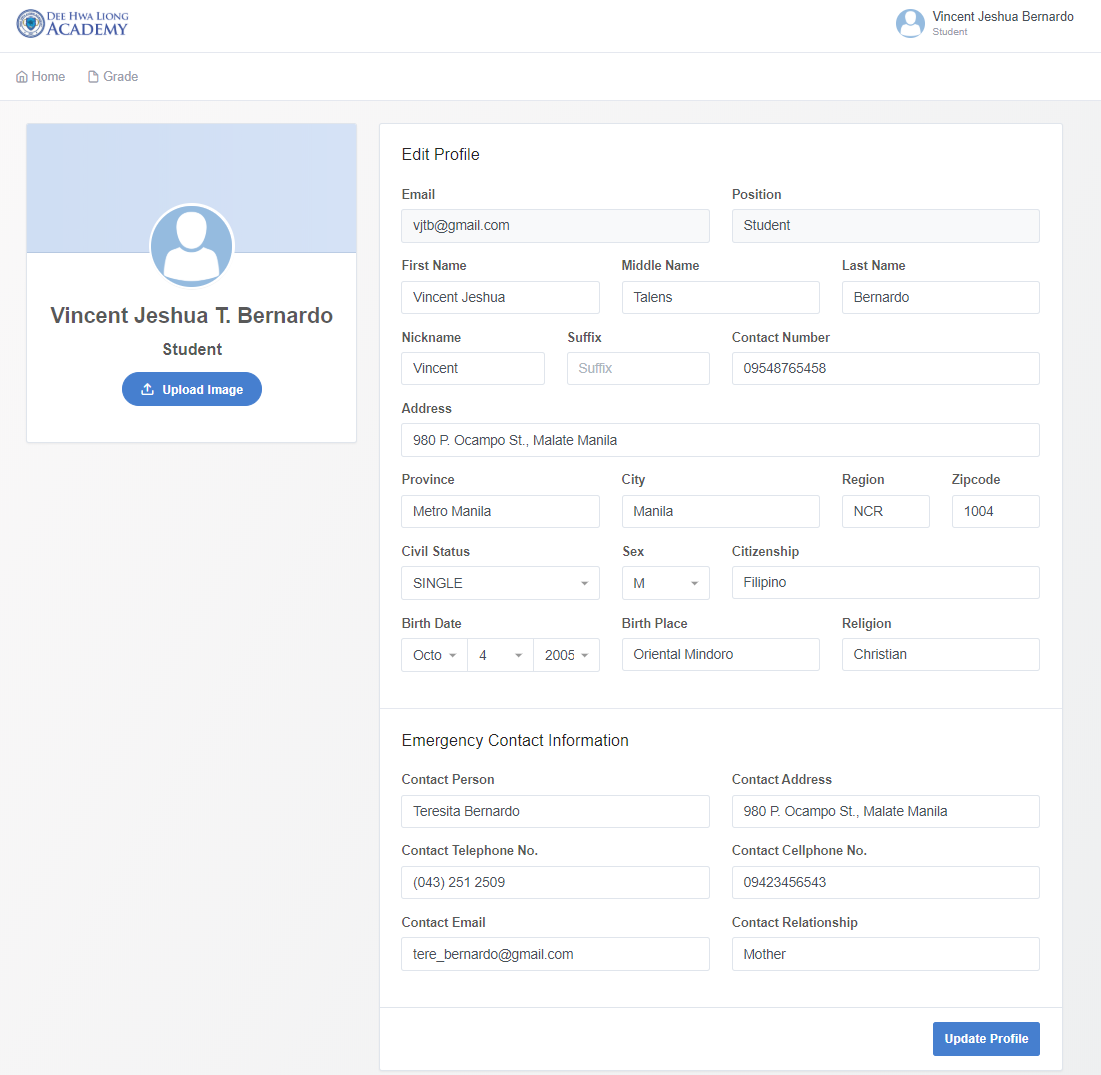
\includegraphics[height=14.5cm]{ViewProfile.png}
  \caption{View/Edit Profile Interface}
  \label{fig:ep}
\end{figure}
\vspace{1cm}
\begin{figure}[H]
  \centering
  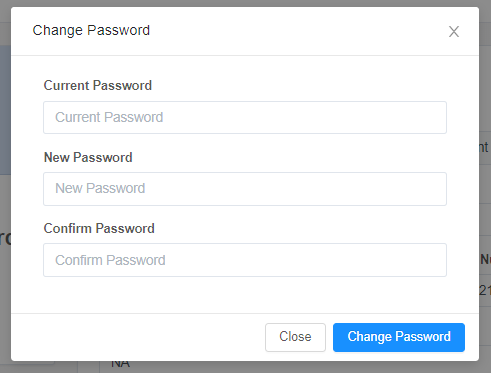
\includegraphics[height=6.5cm]{ChangePassword.png}
  \caption{Change Password Interface}
  \label{fig:cp}
\end{figure}

Figure~\ref{fig:ep} shows the profile of a user. The user can edit his/her personal information. The user can also change password as shown in Figure~\ref{fig:cp}

\subsection{System Administrator}
Figure~\ref{fig:caaal} shows the dashboard page of the System Administrator module. Accounts are created manually, indicating the email, position, first name, middle name, and last name. All user accounts will also be listed in the dashboard. A user account can be deleted if the owner is no longer affiliated with the school or suspended. All records linked with the account will also be deleted.

Figure~\ref{fig:ap} shows the assigning of parents to a given student. Assigning a parent to a student will give the parent access to the student records. 

\vspace{1cm}
\begin{figure}[H]
  \centering
  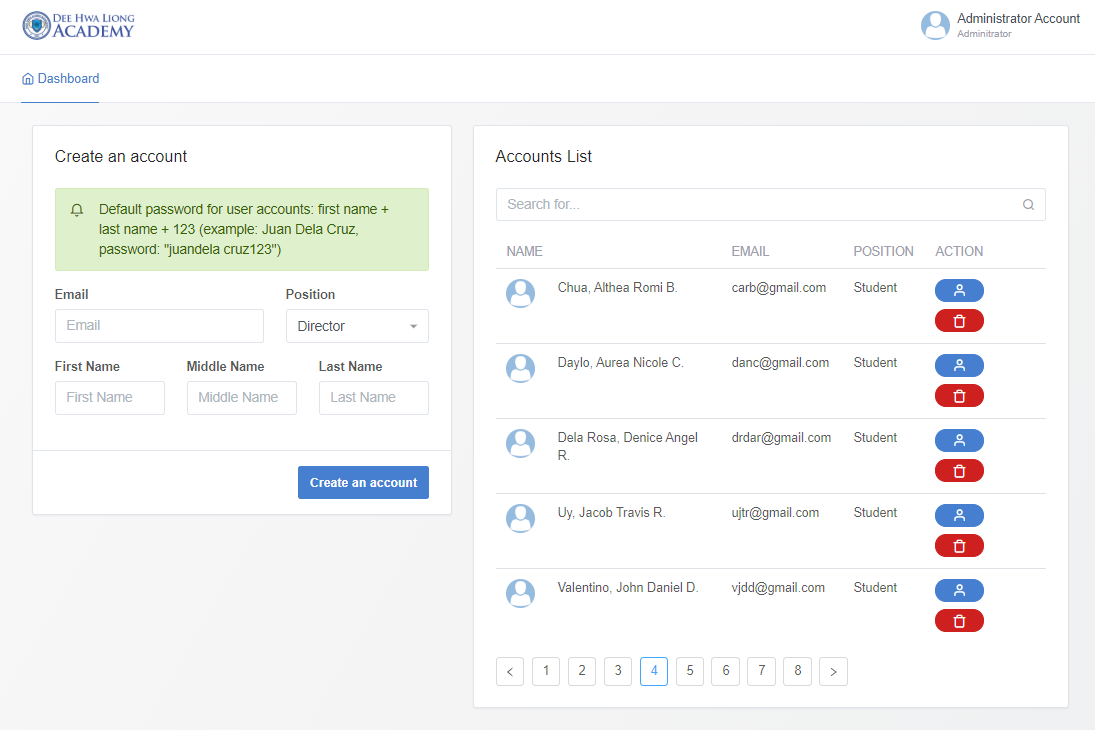
\includegraphics[height=10.5cm]{AdminCreateAccount.png}
  \caption{Create Account and Account List}
  \label{fig:caaal}
\end{figure}
\vspace{1cm}
\begin{figure}[H]
  \centering
  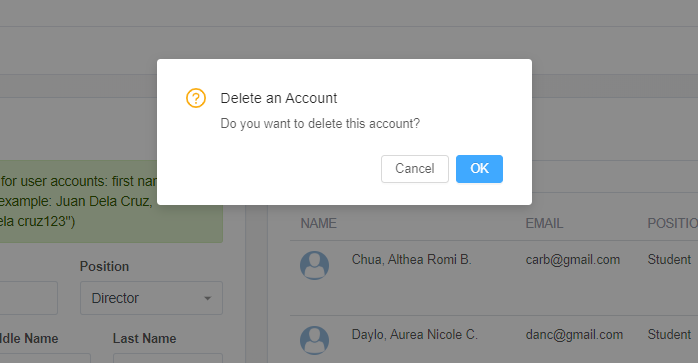
\includegraphics[height=6.5cm]{AccountDeletion.png}
  \caption{Account Deletion}
  \label{fig:ad}
\end{figure}
\vspace{1cm}
\begin{figure}[H]
  \centering
  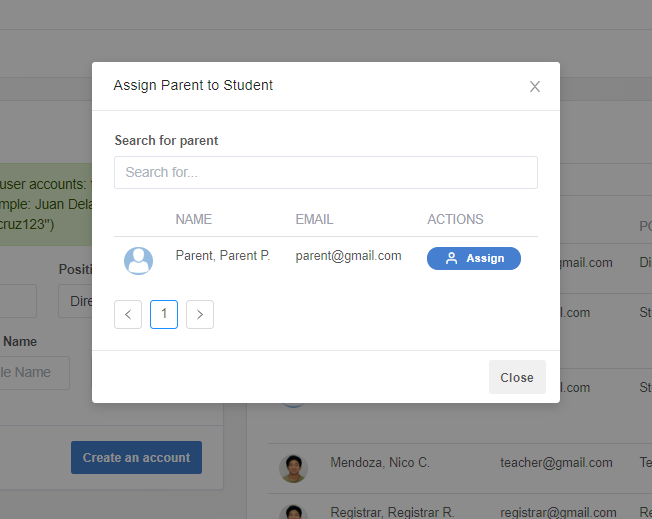
\includegraphics[height=9.5cm]{AssignParent.png}
  \caption{Assign Parent to Student}
  \label{fig:ap}
\end{figure}

\subsection{Director}

Figure~\ref{fig:vsr} shows the view student records interface for both registrar and director. All student records can be viewed from past school years to present. The system provides the condensed grades of each students. By hovering the mouse to a student grade, both have an option to view its corresponding class record. 

Registrar account can generate report cards by section or by student, as shown in Figures~\ref{fig:scrv},~\ref{fig:seccrv}, and ~\ref{fig:grc}.

Both Director and Registrar can view the list and number of students who passed/failed a subject. They can also view the number of honor students per section in a given school year, as shown in Figure~\ref{fig:vpf}.

\vspace{1cm}
\begin{figure}[H]
  \centering
  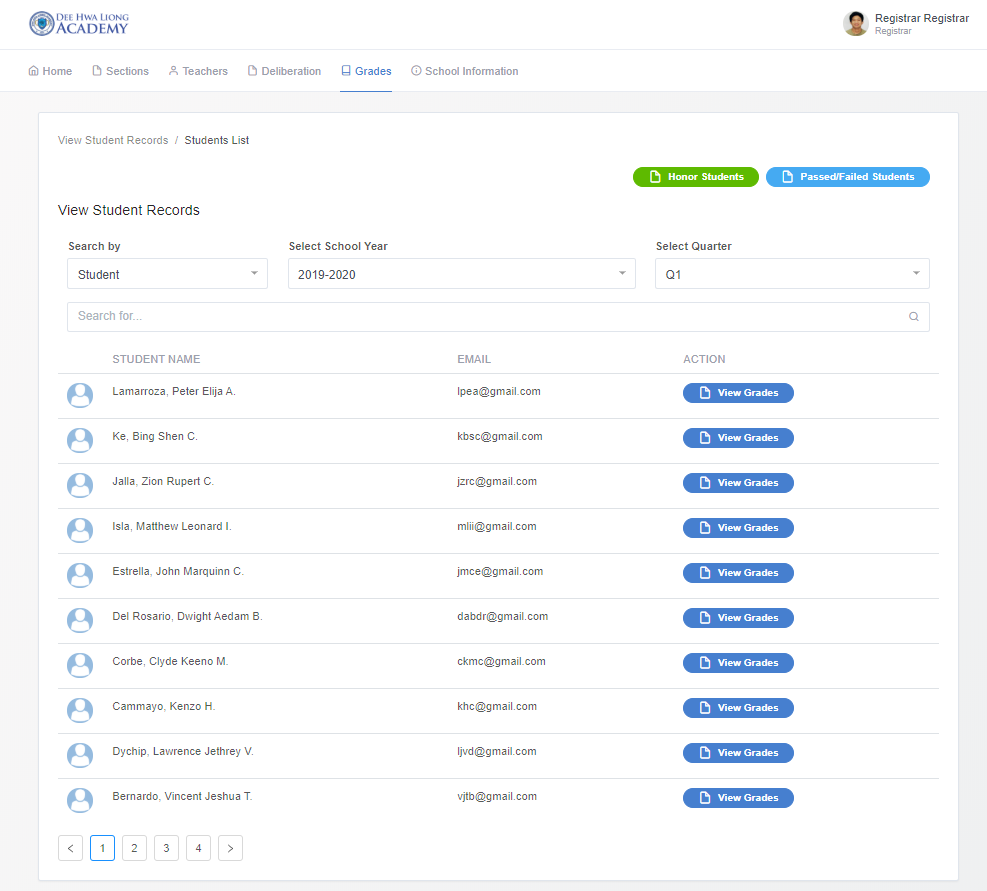
\includegraphics[height=14.5cm]{ViewStudentRecord.png}
  \caption{View Student Record - Student View}
  \label{fig:vsr}
\end{figure}
\vspace{1cm}
\begin{figure}[H]
  \centering
  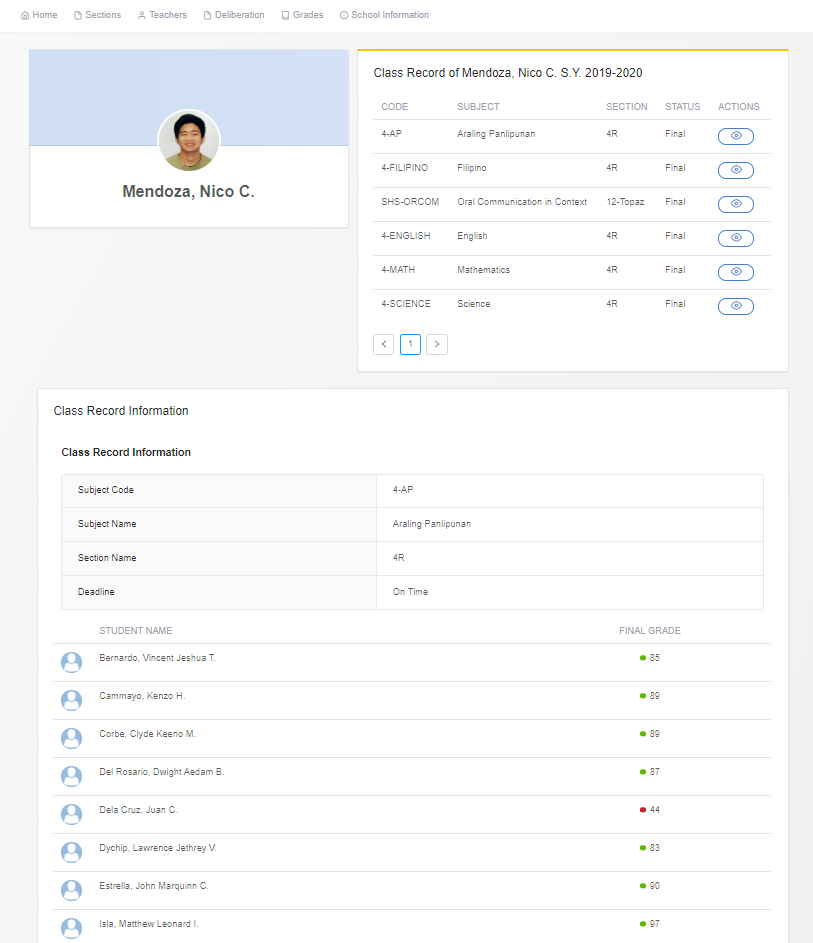
\includegraphics[height=18.5cm]{TeacherCentric.png}
  \caption{Teacher-Centric Record View}
  \label{fig:tcrv}
\end{figure}    
\vspace{1cm}
\begin{figure}[H]
  \centering
  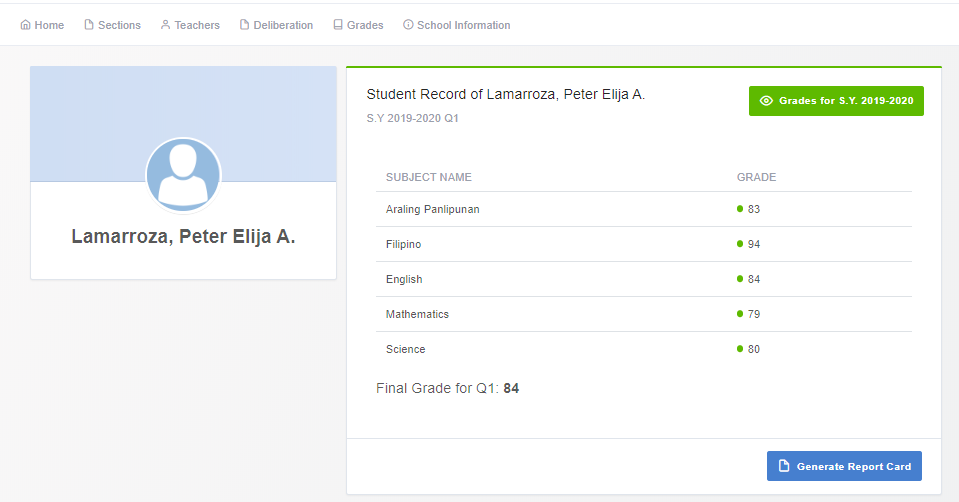
\includegraphics[height=7.5cm]{StudentCentric.png}
  \caption{Student-Centric Record View}
  \label{fig:scrv}
\end{figure}   
\vspace{1cm}
\begin{figure}[H]
  \centering
  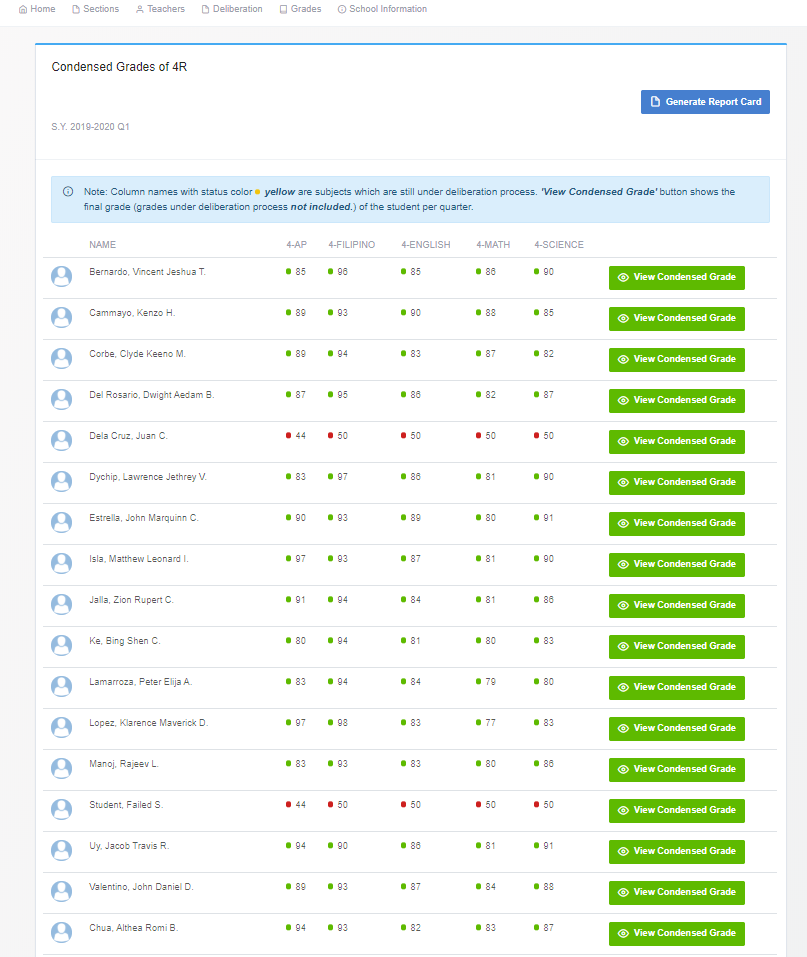
\includegraphics[height=17.5cm]{SectionCentric.png}
  \caption{Section-Centric Record View}
  \label{fig:seccrv}
\end{figure}  
\vspace{1cm}
\begin{figure}[H]
  \centering
  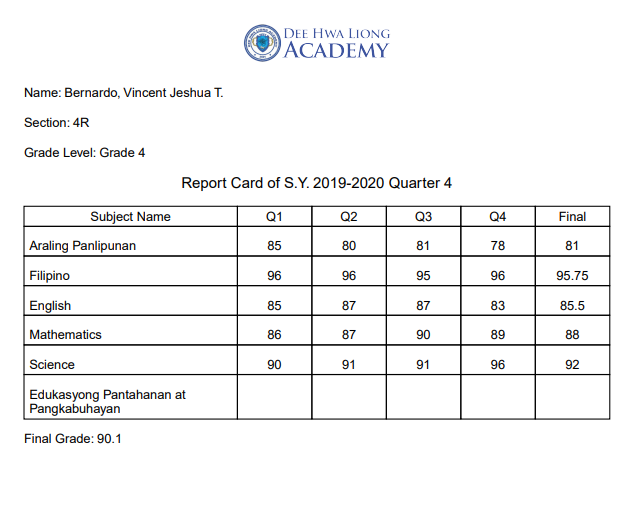
\includegraphics[height=9.5cm]{PrintReportCard.png}
  \caption{Generate Report Card}
  \label{fig:grc}
\end{figure}  
\vspace{1cm}
\begin{figure}[H]
  \centering
  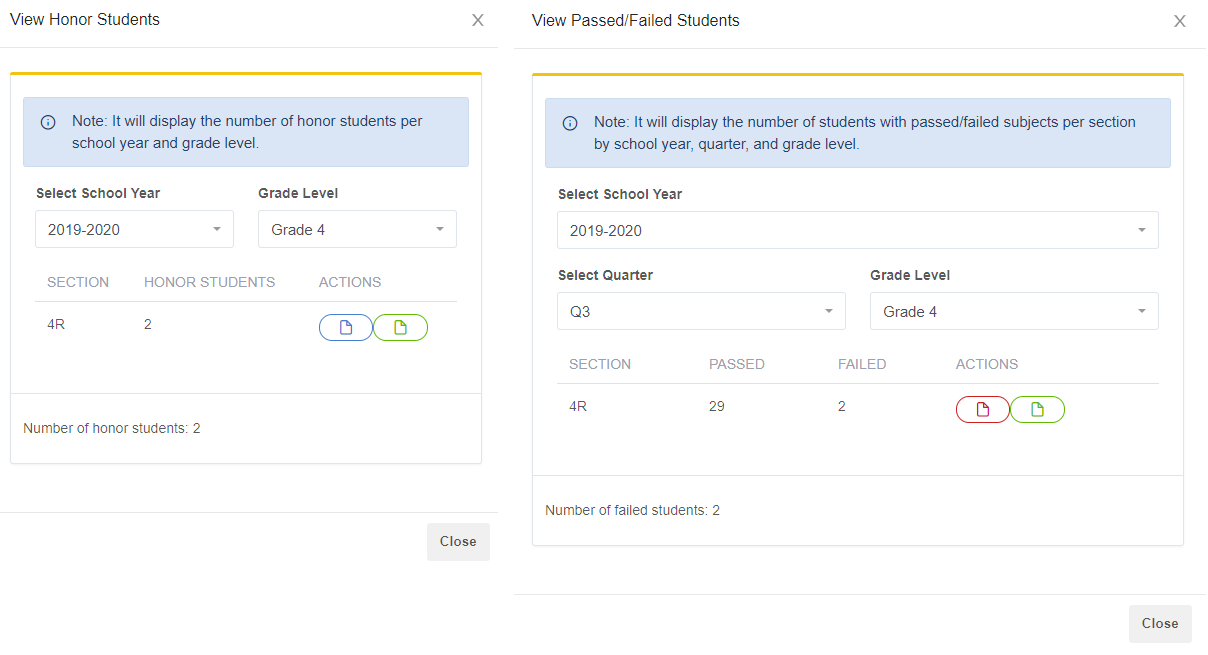
\includegraphics[height=8.9cm]{ViewPassedFailed.png}
  \caption{View Honor Students and Passed/Failed Students}
  \label{fig:vpf}
\end{figure}  

\subsection{Cashier}

Figure~\ref{fig:cd} shows the dashboard page of the cashier module. Cashier can view all student accounts registered in the system. If the student has unpaid balance, the cashier clerk can restrict the account and put a message everytime the student tries to login.
\vspace{1cm}
\begin{figure}[H]
  \centering
  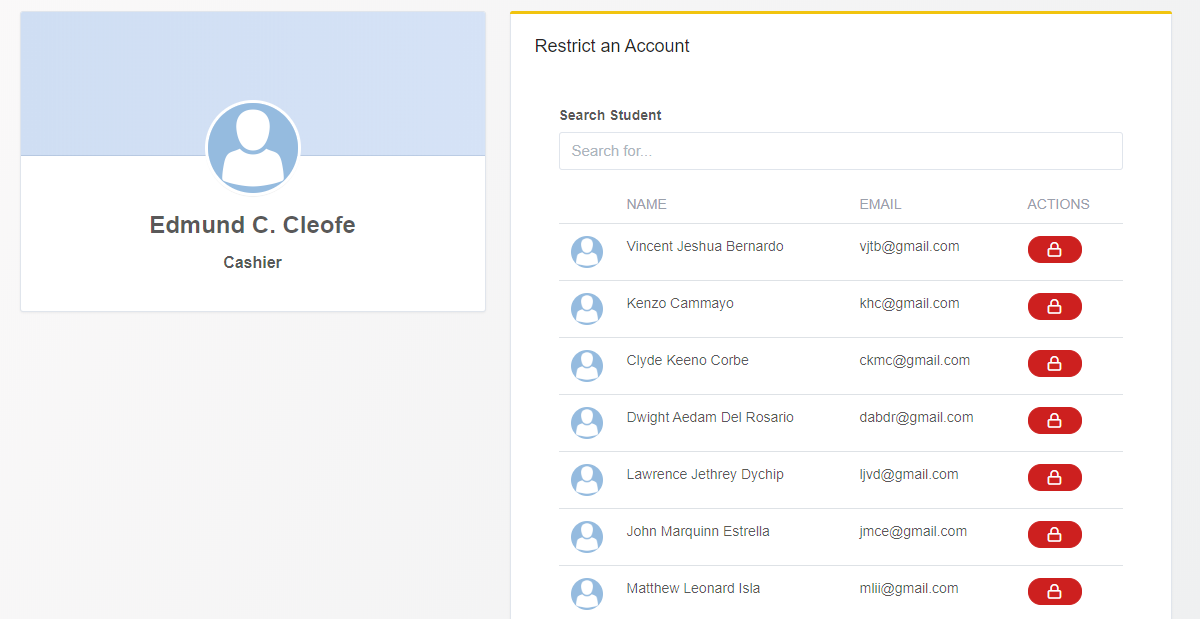
\includegraphics[height=7.5cm]{CashierDashboard.png}
  \caption{Cashier Dashboard}
  \label{fig:cd}
\end{figure}  
\vspace{1cm}
\begin{figure}[H]
  \centering
  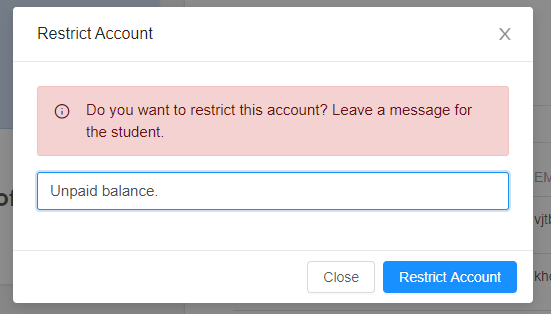
\includegraphics[height=5.5cm]{RestrictAccount.png}
  \caption{Restrict Account}
  \label{fig:ra}
\end{figure}  

\subsection{Registrar}

Figure~\ref{fig:csyc} shows the creation of a school year. Once a school year is created, all user accounts (including teachers and students) will be disabled. A student can only access the system once he/she is already enrolled in a section and has at least one subject enrolled. For the teachers, they can only access the system once they have at least one subject load in the current school year.

\vspace{1cm}
\begin{figure}[H]
  \centering
  
\includegraphics[height=3.0cm]{NoActiveSchoolYear.png}
  \caption{Create School Year Component}
  \label{fig:csyc}
\end{figure}  
\vspace{1cm}
\begin{figure}[H]
  \centering
  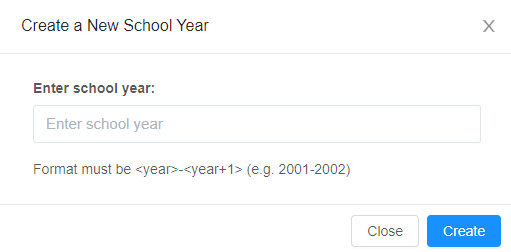
\includegraphics[height=3.5cm]{CreateANewSchoolYear.png}
  \caption{Create School Year Modal}
  \label{fig:csym}
\end{figure}  
Figure~\ref{fig:sl} shows the list of active sections in the current school year. The registrar can edit the name, grade level of each section. The registrar can also delete a section. 

Figure~\ref{fig:esl} shows the list of enrolled students in a section. The registrar can add, or remove students in a given section. The registrar can also view all students enrolled in the previous school year. He/she has the option to import students to the selected section. 

\begin{figure}[H]
  \centering
  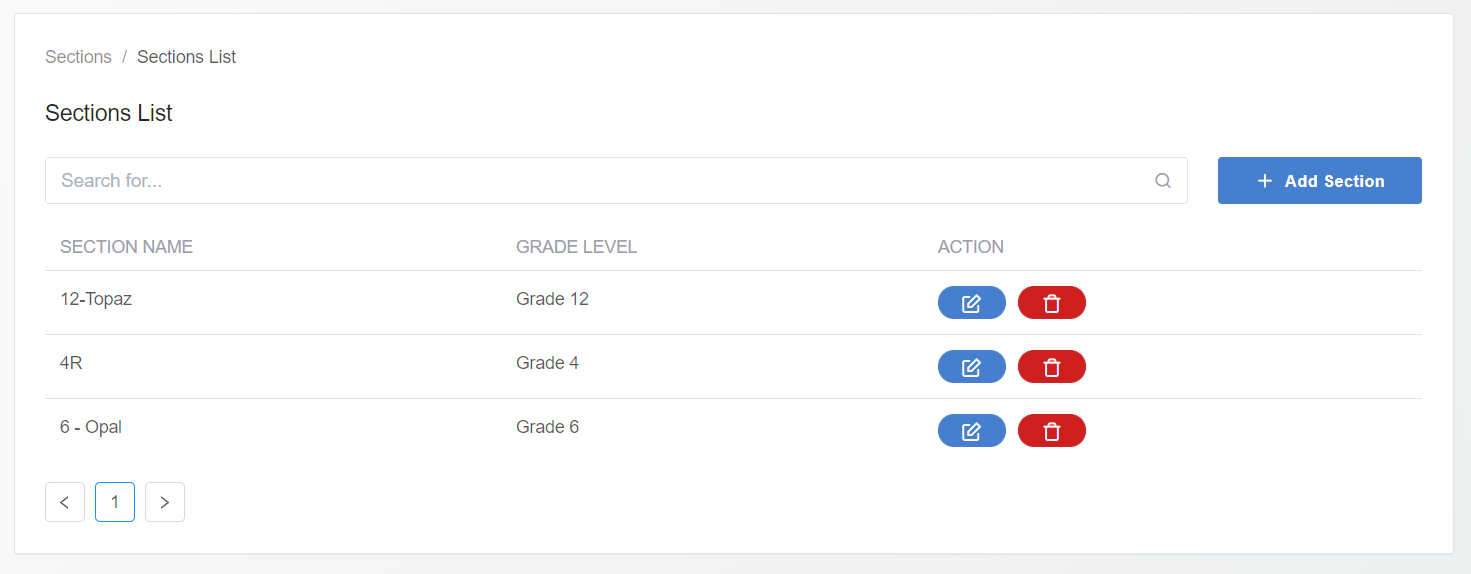
\includegraphics[height=5.5cm]{SectionList.png}
  \caption{Sections List}
  \label{fig:sl}
\end{figure}  
\begin{figure}[H]
  \centering
  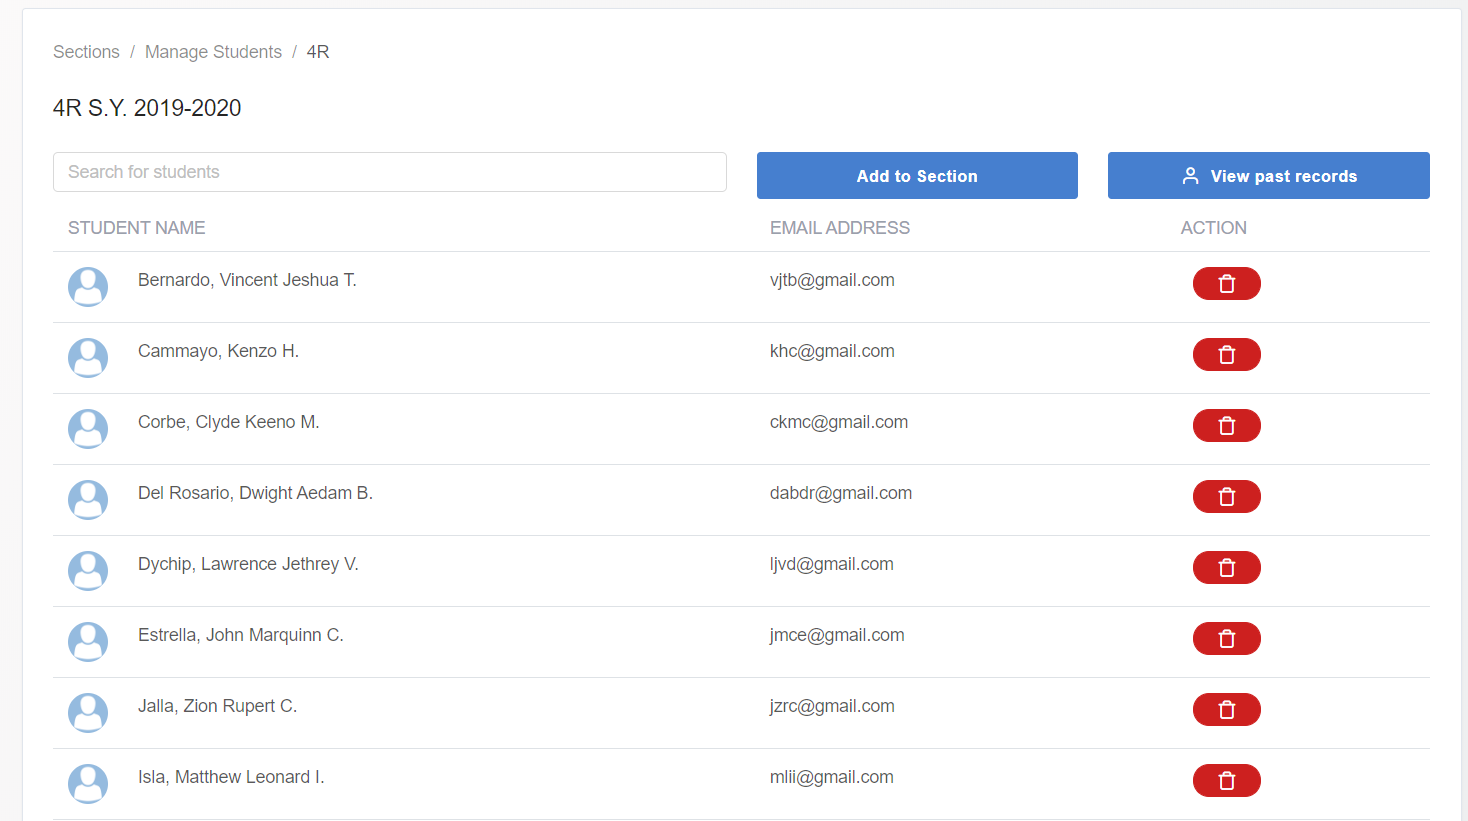
\includegraphics[height=8.5cm]{ManageStudents.png}
  \caption{Enrolled Students List}
  \label{fig:esl}
\end{figure}  
The registrar can assign advisers for each section, as shown in Figure~\ref{fig:aa}. Once a teacher is assigned, they can access the condensed grades of the students enrolled in the section through the system.  Figure~\ref{fig:ansl} shows the 'Assign Subject Load' feature of the system. For assigning a subject load to teachers, the registrar will indicate the grade level, section, and subject that the teacher will teach. Once indicated, the registrar has the option to import all students enrolled in that section or add students manually.  

\begin{figure}[H]
  \centering
  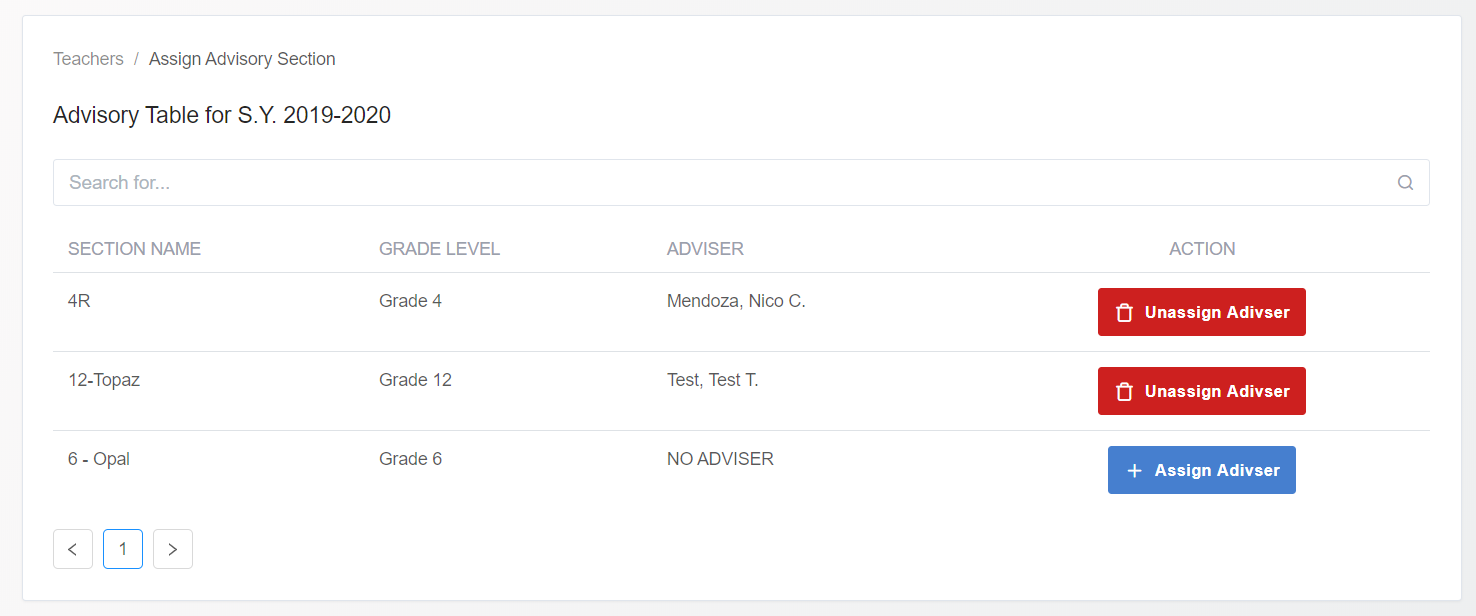
\includegraphics[height=6.5cm]{AssignAdvisers.png}
  \caption{Assign Advisers}
  \label{fig:aa}
\end{figure}  
\begin{figure}[H]
  \centering
  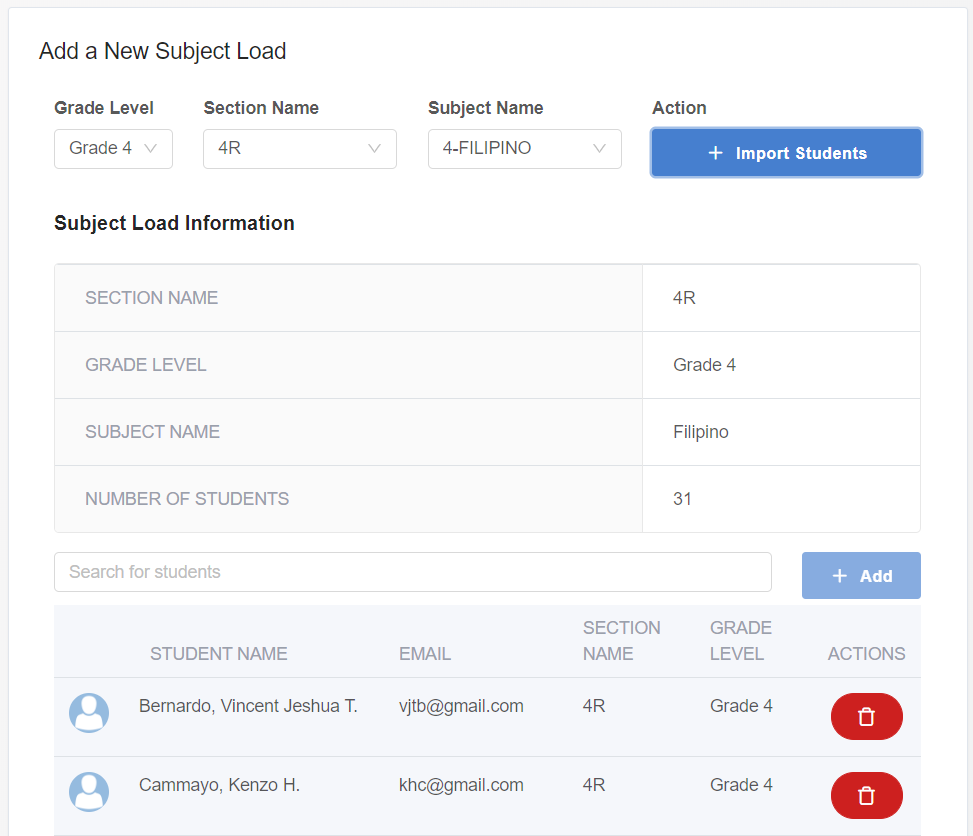
\includegraphics[height=10.5cm]{AddNewSubjectLoad.png}
  \caption{Add New Subject Load}
  \label{fig:ansl}
\end{figure}  
Once a teacher submitted his/her class record for deliberation, the registrar will be able to access the record under the 'Deliberation' tab.  Deliberation process is divided into 2 parts: Individual Deliberation, and Group Deliberation. 

\begin{figure}[H]
  \centering
  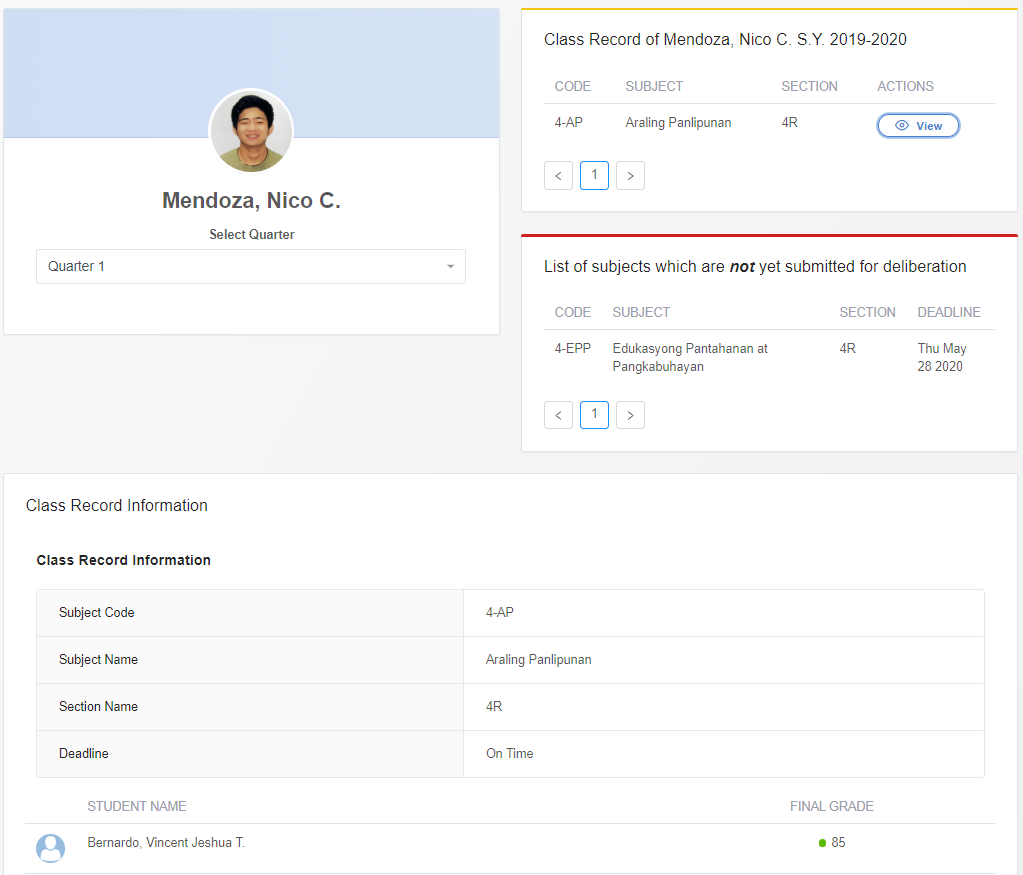
\includegraphics[height=10.5cm]{IndividualDeliberation.png}
  \caption{Deliberation Process}
  \label{fig:dp}
\end{figure}  

For the individual deliberation process, the registrar, and the teacher are expected to meet personally to manually check the class record for possible wrong grade inputs. This time, only the registrar can modify the submitted class record. All changes made by the registrar will be shown in the class record log, as shown in Figure~\ref{fig:crl}.

\begin{figure}[H]
  \centering
  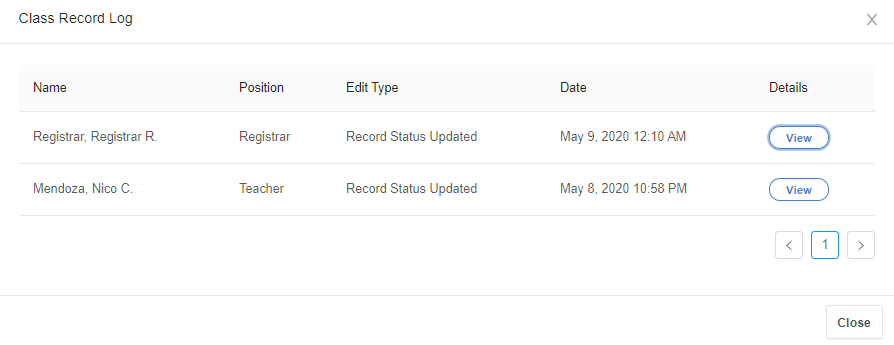
\includegraphics[height=5.5cm]{ClassRecordLog.png}
  \caption{Class Record Log}
  \label{fig:crl}
\end{figure}  

For the group deliberation process, the condensed grades of all students in a section is displayed, as shown in Figure~\ref{fig:gdp}. The registrar can now see the current class standing of the students (including grades under deliberation process). Once everything is finalized, class records can now be submitted for final posting. Once the class records are posted, it will be available for the students and parents to access.  

\begin{figure}[H]
  \centering
  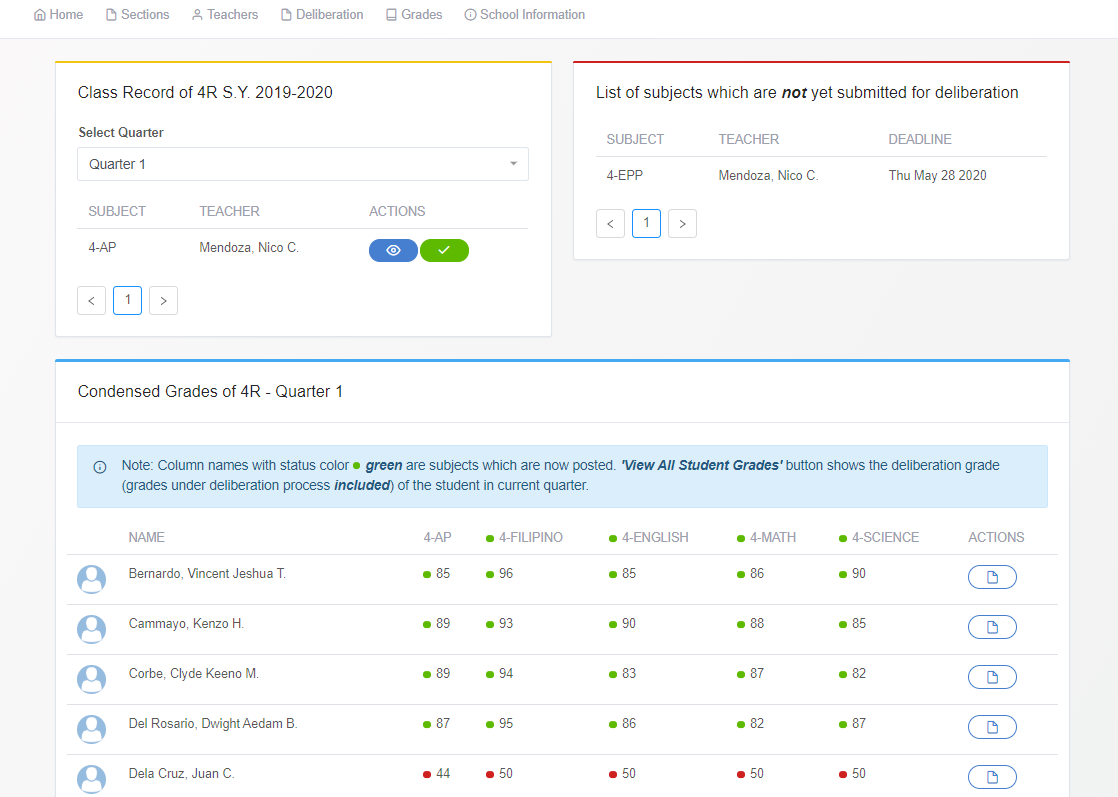
\includegraphics[height=10.5cm]{GroupDeliberation.png}
  \caption{Group Deliberation Process}
  \label{fig:gdp}
\end{figure}  
\subsection{Teacher}

Figure~\ref{fig:tsl} shows the list of subject load of teachers. The teacher can filter the subject load by school year, and quarter. Upon clicking a subject, basic information about the subject load will be displayed such as the Section Name, Grade Level, Subject Name, and the list of enrollled students.

\begin{figure}[H]
  \centering
  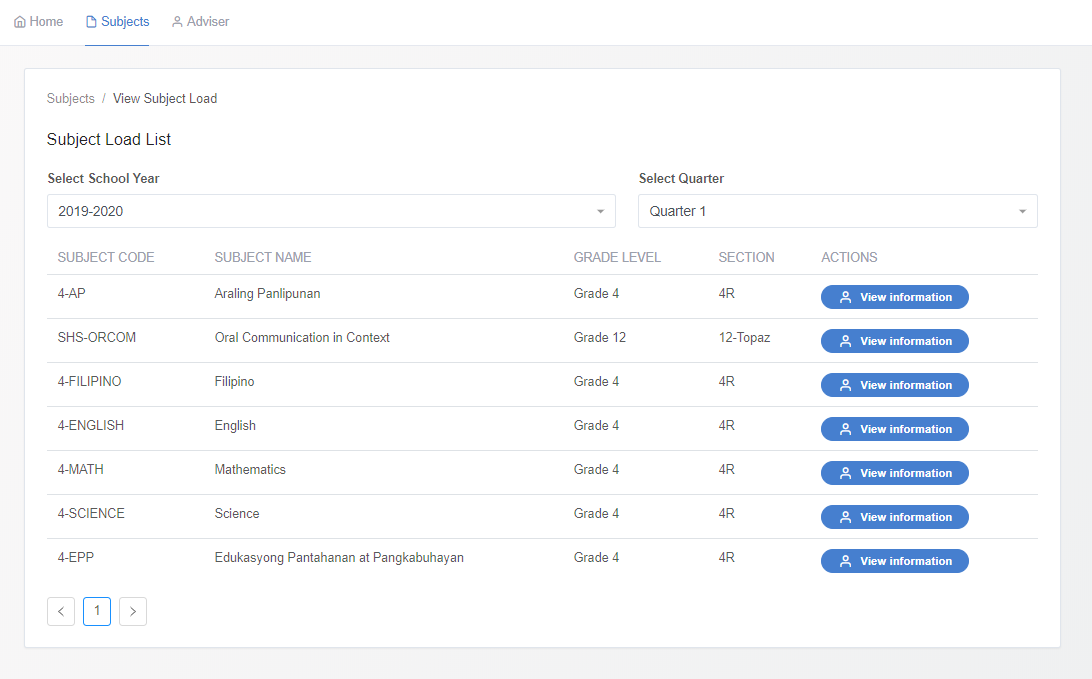
\includegraphics[height=9.5cm]{TeacherSubjectLoad.png}
  \caption{Teacher Subject Load}
  \label{fig:tsl}
\end{figure}  

Figure~\ref{fig:tmg} shows the 'Manage Grades' interface. In this page, the teacher can modify subcomponents in each component (Formative Assessment, Written Works, Performance Task, Quarterly Assessment). The teacher can create and modify the name, and weight of each subcomponent as shown in Figure~\ref{fig:tes}. All subcomponents under a component must accumulate to 100\%, and no negative values are allowed. 

\begin{figure}[H]
  \centering
  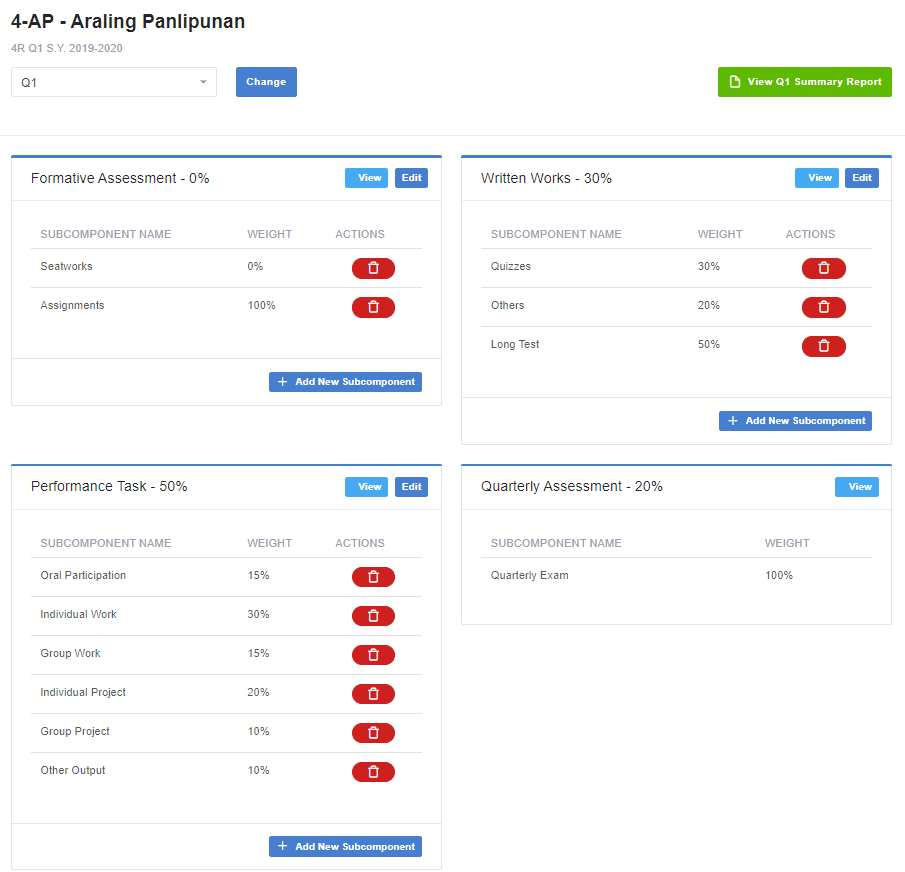
\includegraphics[height=12.5cm]{ManageGrades.png}
  \caption{Teacher Manage Grades}
  \label{fig:tmg}
\end{figure}  

\begin{figure}[H]
  \centering
  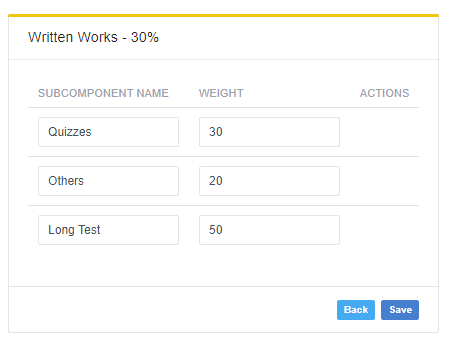
\includegraphics[height=5.5cm]{ModifySubcomponents.png}
  \caption{Teacher Edit Subcomponents}
  \label{fig:tes}
\end{figure}  

Modification of class records can only happen during the 'Encoding' process. After the teacher submitted his/her class record, he/she won't be able to modify its content. However, the teacher can still view the class record logs to see all changes made in the class record.

Figure~\ref{fig:tc} shows the 'Component' interface. In this page, the teacher can view all subcomponents in a given component. It is also an overview of current percentage score of students per subcomponent. The last column shows the average of all scores.

\begin{figure}[H]
  \centering
  \includegraphics[height=7.5cm]{TeacherComponent.png}
  \caption{Teacher Component}
  \label{fig:tc}
\end{figure}  

Figure~\ref{fig:tsc} shows the 'Subcomponent' interface. This is where the teacher can add, modify, or delete records. The system also handles the automatic updating of average scores of all students everytime a record is modified. 

\begin{figure}[H]
  \centering
  \includegraphics[height=7.5cm]{TeacherSubcomponent.png}
  \caption{Teacher Subcomponent}
  \label{fig:tsc}
\end{figure}  

For adding a new record, the teacher will indicate the description of the item, date given, total number of items, and the corresponding scores of each student, as shown in Figure~\ref{fig:anr}. Scores with value of 'E' are considered excused. Scores with value of 'A' are considered absent. 

\begin{figure}[H]
  \centering
  \includegraphics[height=9.5cm]{AddNewRecord.png}
  \caption{Add New Record}
  \label{fig:anr}
\end{figure}  

The teacher can view the summary report of the class record, as shown in Figure~\ref{fig:srpq}. The summary report can be viewed by quarter, or by school year (by semester in SHS subjects). In this page, the actual grade of the student is displayed, along with the transmuted (50\%, 55\%, 60\%) grades. The teacher can choose which transmutation will be used for the final quarter grade, as shown in Figure~\ref{fig:ct}.

\begin{figure}[H]
  \centering
  \includegraphics[height=6.5cm]{SummaryReportPerQ.png}
  \caption{Summary Report Per Quarter}
  \label{fig:srpq}
\end{figure}  
\begin{figure}[H]
  \centering
  \includegraphics[height=6.5cm]{SummaryReport.png}
  \caption{School Year Summary Report}
  \label{fig:sr}
\end{figure}  
\begin{figure}[H]
  \centering
  \includegraphics[height=5.5cm]{ChangeTransmutation.png}
  \caption{Change Transmutation}
  \label{fig:ct}
\end{figure}  

The 'Adviser' tab in the system will be shown if the teacher is also an adviser. The adviser can view the condensed grades of all handled students, as shown in Figure~\ref{fig:asr}.

\begin{figure}[H]
  \centering
  \includegraphics[height=8.5cm]{AdviserStudentRecords.png}
  \caption{Adviser Student Records}
  \label{fig:asr}
\end{figure}  

\subsection{Student}

Once the registrar posted the class record, the condensed grades will be accessible for the students and parents. Figure~\ref{fig:srv} shows the 'Grade' interface of student module. In this page, the student can view his/her grades from past school years to present. The student can also choose which quarter grade to view. The average of all subject grades will also be displayed.

\begin{figure}[H]
  \centering
  \includegraphics[height=9.5cm]{StudentRecord.png}
  \caption{Student Records View}
  \label{fig:srv}
\end{figure}  
\subsection{Parent}

The parent can also access the students' grades linked to his/her account, as shown in Figure~\ref{fig:psrv}. 

\begin{figure}[H]
  \centering
  \includegraphics[height=14.5cm]{ParentStudentRecord.png}
  \caption{Parent Student Records View}
  \label{fig:psrv}
\end{figure}  

\section{Discussions}

Dee Hwa Liong Academy Grade Management System is able to provide convenience to the school by eliminating the needs of manually generating spreadsheet files for the teachers. The registrar module can automatically generate class records just by assigning subject loads to teachers. It is secured by default, since no one can access the class record except the teacher logged in to the system. At the start of the school year, the registrar can create, edit, or delete a section. All students will then be enrolled to these sections using the 'Add Students to Section' feature. This is to ensure that all students which will be included in class records are enrolled. The system has implemented the 'Assign Advisers' feature. Once a teacher is assigned as adviser, he/she can access the condensed grades of all handled students using the system. It allows the teacher to easily monitor the student records in the section he/she is handling. 

Teachers can now easily modify his/her class record. Adding a new subcomponent using spreadsheet files is a tedious process, since there is a fixed number of cells allotted for a single component and adding one would force the editor to adjust the succeeding columns to the right. In the system, the teacher can personalize and add many subcomponents to a component as long as the accumulated weights are equal to 100\%. The teacher can also add, edit, and delete records just like in spreadsheet files, except the system is not prone to data corruption and secured. Once a teacher submitted his/her class record, it is automatically submitted to the registrar for deliberation process. 

All changes made in the class record during the deliberation process is monitored by the system. Any changes (adding, modifying, deleting a subcomponent, adding, modifying, deleting a record, changing weights of a subcomponent, changing the transmutation of the class record, and more) will be displayed in the Class Record Logs. This is to ensure that no unnecessary changes will be made by the registrar or the teacher. Once the class records are finalized, the registrar can submit the grades for final posting. Once posted, the grades will be accessible for the students and parents. 

Students and Parents can now access the grades using the system. They can also view past records from previous school years to present. For the Registrar and Director, they can also access all student records in the system. The Registrar can generate report cards, as well as Advisers.

\section{Conclusions}

Dee Hwa Liong Academy Grade Management System is a web application built to solve bottle neck problems of the school. These bottle neck problems include the preparation and distribution of class records per subject teacher, produce a condensed class record per section, and formating of grades per printing. It also solves the security issues of using spreadsheet files in submission of grades. 

As discussed earlier, before the classes start, the IT head gets all enrolled students, their corresponding section, and the subject load of each teacher from the registrar's office. The spreadsheet files used to record student records are then manually generated, adding the teacher's current load with corresponding students enrolled in that subject and distributed to each teacher. The web application can now automatically generate all class records everytime a registrar assigns a subject load to teacher. All generated class records will automatically reflect on the teacher account. Based on the grade level and subject, component weights will adjust accordingly.  

Keeping track of late submissions is also implemented in the system. The registrar do not have to manually write the date when the grades were submitted. The system will indicate whether the teacher submitted the grades on time or late. 

Submission of class records is now done in the system. Once a class record is submitted for deliberation, it will automatically received by the registrar. As result, there is no need to transfer files through flash drive or facebook messenger. There is only one copy of the class record, thus file duplication is not possible. 

All changes made by the teacher and registrar in the class record is recorded in the system. This is to keep track of all possible changes made during the deliberation process. In effect, the class record will be prone to unauthorized modification.  

Once the teacher has submitted the class record, condensed grades of students are automatically generated using the system. The IT head do not have to compile all teacher-centric records in one spreadsheet file to generate section-centric records. During the deliberation process, the deliberation column will also be shown. Both Director and Registrar can also view the honor students per grade level. They can also view students who failed a subject. 

After the grades are finalized, the registrar can now generate report cards through the system. It eliminates the need of generating student-centric files to produce multiple class records. 

\section{Recommendations}

Dee Hwa Liong Academy Grade Management System has still limitations. It does not cover the grading system from Nursery to Kinder 1 since they use progressive curriculum, and the basis for assessing a student is a checklist.

The system also does not cover the enrollment process of Dee Hwa Liong Academy. All created student acounts are assumed to be enrolled. It can be improved by adding enrollment processes which includes enlistment, and payment. 

It does not track prerequisite subjects. Any students can be enrolled to any subject regardless of his/her grade level. To further improve the web application, it would be better if prerequisite subjects can be defined in the system to avoid unqualified students to be enrolled in a subject. 

A chat feature would also be a great addition to the system. It will allow teachers to directly communicate with the registrar through the system. It might also eliminate the need of personal meeting during individual deliberation process. The implementation would need a socket server and E2EE (end-to-end encryption) is a also must to provide security to the messages.



\bibliographystyle{ieeetr}
\bibliography{biblio}

\twocolumn
\section{Appendix}
\begin{lstlisting}[caption=AccountNotice.js]
     const Sequelize = require( "sequelize" );
     const sequelize = require( "../config/db/database" );
    
     const AccountNotice = sequelize.define(
       "account notice", {
	 accountnoticeID: {
	   type: Sequelize.INTEGER,
	   primaryKey: true,
	   autoIncrement: true
	 },
	 accountID: {
	   type: Sequelize.INTEGER
	 },
	 message: {
	   type: Sequelize.STRING( 100 )
	 }
       }, {
	 freezeTableName: true
       }
     );
    
     module.exports = AccountNotice;
\end{lstlisting}

 \begin{lstlisting}[caption=ActivityLog.js]
 const Sequelize = require("sequelize");
 const sequelize = require("../config/db/database");

 const ActivityLog = sequelize.define(
   "activity log",
   {
     logID: {
       type: Sequelize.INTEGER,
       primaryKey: true,
       autoIncrement: true
     },
     type: {
       type: Sequelize.ENUM(
	 "ADD",
	 "UPDATE",
	 "DELETE",
	 "CHANGE_STATUS",
	 "SUBCOMP_UPDATE",
	 "TRANSMU_UPDATE",
	 "SUBCOMP_ADD",
	 "SUBCOMP_DELETE",
	 "DESC_UPDATE",
	 "TOTAL_UPDATE"
       )
     },
     classRecordID: {
       type: Sequelize.INTEGER
     },
     position: {
       type: Sequelize.STRING
     },
     name: {
       type: Sequelize.STRING
     },
     section: {
       type: Sequelize.STRING
     },
     subject: {
       type: Sequelize.STRING
     },
     timestamp: {
       type: Sequelize.DATE
     },
     quarter: {
       type: Sequelize.STRING
     }
   },
   {
     freezeTableName: true
   }
 );

 module.exports = ActivityLog;

 \end{lstlisting}

 \begin{lstlisting}[caption=AttendanceLog.js]
 const Sequelize = require("sequelize");
 const sequelize = require("../config/db/database");

 const AttendanceLog = sequelize.define(
   "attendance log",
   {
     attendanceID: {
       type: Sequelize.INTEGER,
       primaryKey: true,
       autoIncrement: true
     },
     date: { type: Sequelize.DATE },
     schoolYearID: { type: Sequelize.INTEGER },
     quarter: {
       type: Sequelize.ENUM("Q1", "Q2", "Q3", "Q4")
     },
     month: { type: Sequelize.INTEGER(2) },
     daysPresent: { type: Sequelize.INTEGER(2) },
     daysTardy: { type: Sequelize.INTEGER(2) },
     totalDays: { type: Sequelize.INTEGER(2) },
     teacherID: { type: Sequelize.INTEGER },
     studentID: { type: Sequelize.INTEGER }
   },
   { freezeTableName: true }
 );

 module.exports = AttendanceLog;

 \end{lstlisting}

 \begin{lstlisting}[caption=ClassRecord.js]
 const Sequelize = require("sequelize");
 const sequelize = require("../config/db/database");

 const ClassRecord = sequelize.define(
   "class record",
   {
     classRecordID: {
       type: Sequelize.INTEGER,
       primaryKey: true,
       autoIncrement: true
     },
     dateCreated: {
       type: Sequelize.DATE
     },
     dateModified: {
       type: Sequelize.DATE
     },
     q1Transmu: {
       type: Sequelize.ENUM("60", "55", "50")
     },
     q2Transmu: {
       type: Sequelize.ENUM("60", "55", "50")
     },
     q3Transmu: {
       type: Sequelize.ENUM("60", "55", "50")
     },
     q4Transmu: {
       type: Sequelize.ENUM("60", "55", "50")
     }
   },
   {
     freezeTableName: true
   }
 );

 module.exports = ClassRecord;

 \end{lstlisting}

 \begin{lstlisting}[caption=ClassRecordStatus.js]
 const Sequelize = require("sequelize");
 const sequelize = require("../config/db/database");

 const ClassRecordStatus = sequelize.define(
   "class record status",
   {
     classrecstatusID: {
       type: Sequelize.INTEGER,
       primaryKey: true,
       autoIncrement: true
     },
     classRecordID: {
       type: Sequelize.INTEGER
     },
     q1: {
       type: Sequelize.ENUM("L", "E", "D", "F")
     },
     q2: {
       type: Sequelize.ENUM("L", "E", "D", "F")
     },
     q3: {
       type: Sequelize.ENUM("L", "E", "D", "F")
     },
     q4: {
       type: Sequelize.ENUM("L", "E", "D", "F")
     },
     q1DateSubmitted: {
       type: Sequelize.DATE
     },
     q2DateSubmitted: {
       type: Sequelize.DATE
     },
     q3DateSubmitted: {
       type: Sequelize.DATE
     },
     q4DateSubmitted: {
       type: Sequelize.DATE
     }
   },
   { freezeTableName: true }
 );

 module.exports = ClassRecordStatus;

 \end{lstlisting}

 \begin{lstlisting}[caption=Component.js]
 const Sequelize = require("sequelize");
 const sequelize = require("../config/db/database");

 const Component = sequelize.define(
   "component",
   {
     componentID: {
       type: Sequelize.INTEGER,
       primaryKey: true,
       autoIncrement: true
     },
     subjectID: {
       type: Sequelize.INTEGER
     },
     component: {
       type: Sequelize.ENUM("FA", "WW", "PT", "QE")
     },
     compWeight: {
       type: Sequelize.FLOAT
     }
   },
   { freezeTableName: true }
 );

 module.exports = Component;

 \end{lstlisting}

 \begin{lstlisting}[caption=Grade.js]
 const Sequelize = require("sequelize");
 const sequelize = require("../config/db/database");
 // const LogDetails = require("../models/LogDetails");
 // const utils = require("../utils");

 const Grade = sequelize.define(
   "grade",
   {
     gradeID: {
       type: Sequelize.INTEGER,
       primaryKey: true,
       autoIncrement: true
     },
     description: {
       type: Sequelize.STRING(100)
     },
     dateGiven: {
       type: Sequelize.DATE
     },
     score: {
       type: Sequelize.FLOAT
     },
     total: {
       type: Sequelize.FLOAT
     },
     componentID: {
       type: Sequelize.INTEGER
     },
     subcomponentID: {
       type: Sequelize.INTEGER
     },
     date: {
       type: Sequelize.DATE
     },
     classRecordID: {
       type: Sequelize.INTEGER
     },
     subsectstudID: {
       type: Sequelize.INTEGER
     },
     showLog: {
       type: Sequelize.BOOLEAN
     },
     isUpdated: {
       type: Sequelize.BOOLEAN
     },
     quarter: {
       type: Sequelize.ENUM("Q1", "Q2", "Q3", "Q4")
     },
     attendance: {
       type: Sequelize.ENUM("A", "E", "P")
     }
   },
   {
     freezeTableName: true
   }
 );

 module.exports = Grade;

 \end{lstlisting}

 \begin{lstlisting}[caption=LogDetails.js]
 const Sequelize = require("sequelize");
 const sequelize = require("../config/db/database");

 const LogDetails = sequelize.define(
   "log details",
   {
     logdetailsID: {
       type: Sequelize.INTEGER,
       primaryKey: true,
       autoIncrement: true
     },
     logID: {
       type: Sequelize.INTEGER
     },
     student: {
       type: Sequelize.STRING
     },
     component: {
       type: Sequelize.STRING
     },
     subcomponent: {
       type: Sequelize.STRING
     },
     description: {
       type: Sequelize.STRING
     },
     oldValue: {
       type: Sequelize.FLOAT
     },
     newValue: {
       type: Sequelize.FLOAT
     }
   },
   { freezeTableName: true }
 );

 module.exports = LogDetails;

 \end{lstlisting}

 \begin{lstlisting}[caption=Nonacademic.js]
 const Sequelize = require("sequelize");
 const sequelize = require("../config/db/database");

 const Nonacademic = sequelize.define(
   "nonacademic",
   {
     facultyID: {
       type: Sequelize.INTEGER,
       primaryKey: true,
       autoIncrement: true
     },
     accountID: {
       type: Sequelize.INTEGER
     }
   },
   { freezeTableName: true }
 );

 module.exports = Nonacademic;

 \end{lstlisting}

 \begin{lstlisting}[caption=ParentGuardian.js]
     const Sequelize = require("sequelize");
     const sequelize = require("../config/db/database");
    
     const ParentGuardian = sequelize.define(
       "parent guardian", {
	 parentID: {
	   type: Sequelize.INTEGER,
	   primaryKey: true,
	   autoIncrement: true
	 },
	 accountID: {
	   type: Sequelize.INTEGER
	 },
	 studentIDs: {
	   type: Sequelize.STRING(1000)
	 }
       }, {
	 freezeTableName: true
       }
     );
    
     module.exports = ParentGuardian;
 \end{lstlisting}

 \begin{lstlisting}[caption=SchoolYear.js]
     const Sequelize = require("sequelize");
     const sequelize = require("../config/db/database");
    
     const SchoolYear = sequelize.define(
       "school year",
       {
	 schoolYearID: {
	   type: Sequelize.INTEGER,
	   primaryKey: true,
	   autoIncrement: true
	 },
	 schoolYear: {
	   type: Sequelize.STRING(9)
	 },
	 isActive: {
	   type: Sequelize.BOOLEAN
	 },
	 quarter: {
	   type: Sequelize.ENUM("Q1", "Q2", "Q3", "Q4"),
	   defaultValue: "Q1"
	 }
       },
       { freezeTableName: true }
     );
    
     module.exports = SchoolYear;
	
 \end{lstlisting}

 \begin{lstlisting}[caption=Section.js]
     const Sequelize = require("sequelize");
     const sequelize = require("../config/db/database");
    
     const Section = sequelize.define(
       "section",
       {
	 sectionID: {
	   type: Sequelize.INTEGER,
	   primaryKey: true,
	   autoIncrement: true
	 },
	 sectionName: {
	   type: Sequelize.STRING(100)
	 },
	 gradeLevel: {
	   type: Sequelize.ENUM(
	     "N",
	     "K1",
	     "K2",
	     "G1",
	     "G2",
	     "G3",
	     "G4",
	     "G5",
	     "G6",
	     "G7",
	     "G8",
	     "G9",
	     "G10",
	     "G11",
	     "G12"
	   )
	 },
	 archived: {
	   type: Sequelize.BOOLEAN,
	   defaultValue: 0
	 }
       },
       { freezeTableName: true }
     );
    
     module.exports = Section;
    
 \end{lstlisting}

 \begin{lstlisting}[caption=Student.js]
     const Sequelize = require("sequelize");
     const sequelize = require("../config/db/database");
    
     const Student = sequelize.define(
       "student",
       {
	 studentID: {
	   type: Sequelize.INTEGER,
	   primaryKey: true,
	   autoIncrement: true
	 },
	 accountID: {
	   type: Sequelize.INTEGER
	 },
	 fatherName: {
	   type: Sequelize.STRING(30)
	 },
	 fatherAddress: {
	   type: Sequelize.STRING(30)
	 },
	 fatherEmail: {
	   type: Sequelize.STRING(30)
	 },
	 fatherOccupation: {
	   type: Sequelize.STRING(30)
	 },
	 fatherEmployer: {
	   type: Sequelize.STRING(30)
	 },
	 fatherBusinessAdd: {
	   type: Sequelize.STRING(30)
	 },
	 fatherOfficeNum: {
	   type: Sequelize.STRING(30)
	 },
	 motherName: {
	   type: Sequelize.STRING(30)
	 },
	 motherAddress: {
	   type: Sequelize.STRING(30)
	 },
	 motherEmail: {
	   type: Sequelize.STRING(30)
	 },
	 motherOccupation: {
	   type: Sequelize.STRING(30)
	 },
	 motherEmployer: {
	   type: Sequelize.STRING(30)
	 },
	 motherBusinessAdd: {
	   type: Sequelize.STRING(30)
	 },
	 motherOfficeNum: {
	   type: Sequelize.STRING(30)
	 }
       },
       { freezeTableName: true }
     );
    
     module.exports = Student;    
 \end{lstlisting}

 \begin{lstlisting}[caption=StudentFinalGrade.js]
     const Sequelize = require("sequelize");
     const sequelize = require("../config/db/database");
    
     const StudentFinalGrade = sequelize.define(
       "student final grade",
    
       {
	 finalGradeID: {
	   type: Sequelize.INTEGER,
	   primaryKey: true,
	   autoIncrement: true
	 },
	 schoolYearID: {
	   type: Sequelize.INTEGER
	 },
	 studsectID: {
	   type: Sequelize.INTEGER
	 },
	 grade: {
	   type: Sequelize.FLOAT
	 }
       },
       {
	 freezeTableName: true
       }
     );
    
     module.exports = StudentFinalGrade;    
 \end{lstlisting}

 \begin{lstlisting}[caption=StudentGrades.js]
     const Sequelize = require("sequelize");
     const sequelize = require("../config/db/database");
    
     const StudentGrades = sequelize.define(
       "student grades",
       {
	 studentgradesID: {
	   type: Sequelize.INTEGER,
	   primaryKey: true,
	   autoIncrement: true
	 },
	 studsectID: {
	   type: Sequelize.INTEGER
	 },
	 schoolYearID: {
	   type: Sequelize.INTEGER
	 },
	 quarter: {
	   type: Sequelize.ENUM("Q1", "Q2", "Q3", "Q4")
	 },
	 grade: {
	   type: Sequelize.FLOAT
	 }
       },
       { freezeTableName: true }
     );
    
     module.exports = StudentGrades;    
 \end{lstlisting}

 \begin{lstlisting}[caption=StudentSection.js]
     const Sequelize = require("sequelize");
     const sequelize = require("../config/db/database");
    
     const StudentSection = sequelize.define(
       "student section",
       {
	 studsectID: {
	   type: Sequelize.INTEGER,
	   primaryKey: true,
	   autoIncrement: true
	 },
	 studentID: {
	   type: Sequelize.INTEGER
	 },
	 sectionID: {
	   type: Sequelize.INTEGER
	 },
	 schoolYearID: {
	   type: Sequelize.INTEGER
	 }
       },
       { freezeTableName: true }
     );
    
     module.exports = StudentSection;    
 \end{lstlisting}

 \begin{lstlisting}[caption=StudentSubjectGrades.js]
     const Sequelize = require("sequelize");
     const sequelize = require("../config/db/database");
    
     const StudentSubjectGrades = sequelize.define(
       "student subject grades",
       {
	 studsubjgradesID: {
	   type: Sequelize.INTEGER,
	   primaryKey: true,
	   autoIncrement: true
	 },
	 subsectstudID: {
	   type: Sequelize.INTEGER
	 },
	 classRecordID: {
	   type: Sequelize.INTEGER
	 },
	 q1FinalGrade: {
	   type: Sequelize.FLOAT,
	   defaultValue: -1
	 },
	 q2FinalGrade: {
	   type: Sequelize.FLOAT,
	   defaultValue: -1
	 },
	 q3FinalGrade: {
	   type: Sequelize.FLOAT,
	   defaultValue: -1
	 },
	 q4FinalGrade: {
	   type: Sequelize.FLOAT,
	   defaultValue: -1
	 },
	 ave: {
	   type: Sequelize.FLOAT,
	   defaultValue: -1
	 }
       },
       { freezeTableName: true }
     );
    
     module.exports = StudentSubjectGrades;    
 \end{lstlisting}

 \begin{lstlisting}[caption=StudentWeightedScore.js]
     const Sequelize = require("sequelize");
     const sequelize = require("../config/db/database");
    
     const StudentWeightedScore = sequelize.define(
       "student weighted score",
       {
	 weightedScoreID: {
	   type: Sequelize.INTEGER,
	   primaryKey: true,
	   autoIncrement: true
	 },
	 subsectstudID: {
	   type: Sequelize.INTEGER
	 },
	 classRecordID: {
	   type: Sequelize.INTEGER
	 },
	 faWS: {
	   type: Sequelize.FLOAT
	 },
	 wwWS: {
	   type: Sequelize.FLOAT
	 },
	 ptWS: {
	   type: Sequelize.FLOAT
	 },
	 qeWS: {
	   type: Sequelize.FLOAT
	 },
	 actualGrade: {
	   type: Sequelize.FLOAT,
	   defaultValue: -1
	 },
	 transmutedGrade50: {
	   type: Sequelize.FLOAT,
	   defaultValue: -1
	 },
	 transmutedGrade55: {
	   type: Sequelize.FLOAT,
	   defaultValue: -1
	 },
	 transmutedGrade60: {
	   type: Sequelize.FLOAT,
	   defaultValue: -1
	 },
	 quarter: {
	   type: Sequelize.ENUM("Q1", "Q2", "Q3", "Q4")
	 }
       },
       { freezeTableName: true }
     );
    
     module.exports = StudentWeightedScore;    
 \end{lstlisting}

 \begin{lstlisting}[caption=Subcomponent.js]
     const Sequelize = require("sequelize");
     const sequelize = require("../config/db/database");
    
     const Subcomponent = sequelize.define(
       "subcomponent",
       {
	 subcompID: {
	   type: Sequelize.INTEGER,
	   primaryKey: true,
	   autoIncrement: true
	 },
	 classRecordID: {
	   type: Sequelize.INTEGER
	 },
	 name: {
	   type: Sequelize.STRING(50)
	 },
	 componentID: {
	   type: Sequelize.INTEGER
	 },
	 compWeight: {
	   type: Sequelize.FLOAT
	 },
	 quarter: {
	   type: Sequelize.ENUM("Q1", "Q2", "Q3", "Q4")
	 }
       },
       { freezeTableName: true }
     );
    
     module.exports = Subcomponent;    
 \end{lstlisting}

 \begin{lstlisting}[caption=Subject.js]
     const Sequelize = require("sequelize");
     const sequelize = require("../config/db/database");
    
     const Subject = sequelize.define(
       "subject",
       {
	 subjectID: {
	   type: Sequelize.INTEGER,
	   primaryKey: true,
	   autoIncrement: true
	 },
	 subjectCode: {
	   type: Sequelize.STRING
	 },
	 subjectName: {
	   type: Sequelize.STRING
	 },
	 archived: {
	   type: Sequelize.BOOLEAN,
	   defaultValue: 0
	 },
	 subjectType: {
	   type: Sequelize.ENUM(
	     "N",
	     "K1",
	     "K2",
	     "G1",
	     "G2",
	     "G3",
	     "G4",
	     "G5",
	     "G6",
	     "G7",
	     "G8",
	     "G9",
	     "G10",
	     "CORE",
	     "ACAD-APPLIED",
	     "ACAD-SPECIALIZED",
	     "TVL-APPLIED",
	     "TVL-SPECIALIZED",
	     "SPORTS-APPLIED",
	     "SPORTS-SPECIALIZED",
	     "AAD-APPLIED",
	     "AAD-SPECIALIZED"
	   )
	 }
       },
       { freezeTableName: true }
     );
    
     module.exports = Subject;    
 \end{lstlisting}

 \begin{lstlisting}[caption=SubjectSection.js]
     const Sequelize = require("sequelize");
     const sequelize = require("../config/db/database");
    
     const SubjectSection = sequelize.define(
       "subject section",
       {
	 subsectID: {
	   type: Sequelize.INTEGER,
	   primaryKey: true,
	   autoIncrement: true
	 },
	 subjectID: {
	   type: Sequelize.INTEGER
	 },
	 sectionID: {
	   type: Sequelize.INTEGER
	 },
	 teacherID: {
	   type: Sequelize.INTEGER
	 },
	 schoolYearID: {
	   type: Sequelize.INTEGER
	 },
	 subjectType: {
	   type: Sequelize.ENUM("NON_SHS", "1ST_SEM", "2ND_SEM")
	 },
	 classRecordID: {
	   type: Sequelize.INTEGER
	 }
       },
       { freezeTableName: true }
     );
    
     module.exports = SubjectSection;    
 \end{lstlisting}

 \begin{lstlisting}[caption=SubjectSectionStudent.js]
     const Sequelize = require("sequelize");
     const sequelize = require("../config/db/database");
    
     const SubjectSectionStudent = sequelize.define(
       "subject section student",
       {
	 subsectstudID: {
	   type: Sequelize.INTEGER,
	   primaryKey: true,
	   autoIncrement: true
	 },
	 studsectID: {
	   type: Sequelize.INTEGER
	 },
	 subsectID: {
	   type: Sequelize.INTEGER
	 }
       },
       {
	 freezeTableName: true
       }
     );
    
     module.exports = SubjectSectionStudent;    
 \end{lstlisting}

 \begin{lstlisting}[caption=SubmissionDeadline.js]
     const Sequelize = require("sequelize");
     const sequelize = require("../config/db/database");
    
     const SubmissionDeadline = sequelize.define(
       "submission deadline",
       {
	 deadlineID: {
	   type: Sequelize.INTEGER,
	   primaryKey: true,
	   autoIncrement: true
	 },
	 teacherID: {
	   type: Sequelize.INTEGER
	 },
	 dateSet: {
	   type: Sequelize.DATE
	 },
	 deadline: {
	   type: Sequelize.DATE
	 },
	 isActive: {
	   type: Sequelize.BOOLEAN
	 }
       },
       { freezeTableName: true }
     );
    
     module.exports = SubmissionDeadline;    
 \end{lstlisting}

 \begin{lstlisting}[caption=Teacher.js]
     const Sequelize = require("sequelize");
     const sequelize = require("../config/db/database");
    
     const Teacher = sequelize.define(
       "teacher",
       {
	 teacherID: {
	   type: Sequelize.INTEGER,
	   primaryKey: true,
	   autoIncrement: true
	 },
	 accountID: {
	   type: Sequelize.INTEGER
	 },
	 isAdviser: {
	   type: Sequelize.BOOLEAN
	 }
       },
       { freezeTableName: true }
     );
    
     module.exports = Teacher;    
 \end{lstlisting}

 \begin{lstlisting}[caption=TeacherSection.js]
     const Sequelize = require("sequelize");
     const sequelize = require("../config/db/database");
    
     const TeacherSection = sequelize.define(
       "teacher section",
       {
	 teachersectionID: {
	   type: Sequelize.INTEGER,
	   primaryKey: true,
	   autoIncrement: true
	 },
	 sectionID: { type: Sequelize.INTEGER },
	 schoolYearID: { type: Sequelize.INTEGER },
	 teacherID: { type: Sequelize.INTEGER }
       },
       { freezeTableName: true }
     );
    
     module.exports = TeacherSection;    
 \end{lstlisting}

 \begin{lstlisting}[caption=UserAcount.js]
     const Sequelize = require("sequelize");
     const sequelize = require("../config/db/database");
    
     const UserAccount = sequelize.define(
       "user account", {
	 accountID: {
	   type: Sequelize.INTEGER,
	   primaryKey: true,
	   autoIncrement: true
	 },
	 email: {
	   type: Sequelize.STRING
	 },
	 password: {
	   type: Sequelize.STRING.BINARY
	 },
	 isActive: {
	   type: Sequelize.BOOLEAN
	 },
	 position: {
	   type: Sequelize.BOOLEAN
	 },
	 firstName: {
	   type: Sequelize.STRING
	 },
	 lastName: {
	   type: Sequelize.STRING
	 },
	 middleName: {
	   type: Sequelize.STRING
	 },
	 suffix: {
	   type: Sequelize.STRING(10)
	 },
	 nickname: {
	   type: Sequelize.STRING(50)
	 },
	 imageUrl: {
	   type: Sequelize.STRING
	 },
	 contactNum: {
	   type: Sequelize.STRING(11)
	 },
	 address: {
	   type: Sequelize.STRING(50)
	 },
	 province: {
	   type: Sequelize.STRING(20)
	 },
	 city: {
	   type: Sequelize.STRING(25)
	 },
	 region: {
	   type: Sequelize.STRING(15)
	 },
	 zipcode: {
	   type: Sequelize.STRING(4)
	 },
	 civilStatus: {
	   type: Sequelize.ENUM("SINGLE", "MARRIED", "WIDOWED", "OTHERS")
	 },
	 sex: {
	   type: Sequelize.ENUM("M", "F")
	 },
	 citizenship: {
	   type: Sequelize.STRING(20)
	 },
	 birthDate: {
	   type: Sequelize.DATE
	 },
	 birthPlace: {
	   type: Sequelize.STRING(25)
	 },
	 religion: {
	   type: Sequelize.STRING(20)
	 },
	 emergencyName: {
	   type: Sequelize.STRING(30)
	 },
	 emergencyAddress: {
	   type: Sequelize.STRING(50)
	 },
	 emergencyTelephone: {
	   type: Sequelize.STRING(50)
	 },
	 emergencyCellphone: {
	   type: Sequelize.STRING(50)
	 },
	 emergencyEmail: {
	   type: Sequelize.STRING(30)
	 },
	 emergencyRelationship: {
	   type: Sequelize.STRING(15)
	 }
       }, {
	 freezeTableName: true,
	 paranoid: true
       }
     );
    
     module.exports = UserAccount;
 \end{lstlisting}

 \begin{lstlisting}[caption=erd.js]
     // Import Models (Database table names)
     const UserAccount = require("../models/UserAccount");
     const Nonacademic = require("../models/Nonacademic");
     const Student = require("../models/Student");
     const ParentGuardian = require("../models/ParentGuardian");
     const Teacher = require("../models/Teacher");
     const Grade = require("../models/Grade");
     const Section = require("../models/Section");
     const Subject = require("../models/Subject");
     const TeacherSection = require("../models/TeacherSection");
     const AttendanceLog = require("../models/AttendanceLog");
     const SubmissionDeadline = require("../models/SubmissionDeadline");
     const SubjectSection = require("../models/SubjectSection");
     const SubjectSectionStudent = require("../models/SubjectSectionStudent");
     const Component = require("../models/Component");
     const StudentWeightedScore = require("../models/StudentWeightedScore");
     const ClassRecord = require("../models/ClassRecord");
     const Subcomponent = require("../models/Subcomponent");
     const AccountNotice = require("../models/AccountNotice");
     const SchoolYear = require("../models/SchoolYear");
     const StudentSection = require("../models/StudentSection");
     const StudentSubjectGrades = require("../models/StudentSubjectGrades");
     const ActivityLog = require("../models/ActivityLog");
     const LogDetails = require("../models/LogDetails");
     const ClassRecordStatus = require("../models/ClassRecordStatus");
     const StudentGrades = require("../models/StudentGrades");
     const StudentFinalGrade = require("../models/StudentFinalGrade");
     const utils = require("../utils");
    
     const useraccountERD = async function() {
       // user account ERD
    
       await UserAccount.hasOne(Nonacademic, {
	 foreignKey: "accountID"
       });
       await UserAccount.hasOne(Student, {
	 foreignKey: "accountID"
       });
       await UserAccount.hasOne(ParentGuardian, {
	 foreignKey: "accountID"
       });
       await UserAccount.hasOne(Teacher, {
	 foreignKey: "accountID"
       });
       await UserAccount.sync({
	 force: false
       }).then(() => {
	 console.log("user account table created/synced");
	 Nonacademic.sync({
	   force: false
	 }).then(() => {
	   console.log("nonacademic table created/synced");
	 });
	 Student.sync({
	   force: false
	 }).then(() => {
	   console.log("student table created/synced");
	 });
	 ParentGuardian.sync({
	   force: false
	 }).then(() => {
	   console.log("parent guardian table created/synced");
	 });
	 Teacher.sync({
	   force: false
	 }).then(() => {
	   console.log("teacher table created/synced");
	 });
       });
     };
    
     const subjectsectionERD = async function() {
       //subject section erd
       await SchoolYear.sync({
	 force: false
       });
       await Section.hasMany(SubjectSection, {
	 foreignKey: "sectionID"
       });
       await Teacher.hasMany(SubjectSection, {
	 foreignKey: "teacherID"
       });
       await Subject.hasMany(SubjectSection, {
	 foreignKey: "subjectID"
       });
       await StudentSection.hasMany(SubjectSectionStudent, {
	 foreignKey: "studsectID"
       });
       await SubjectSection.hasMany(SubjectSectionStudent, {
	 foreignKey: "subsectID"
       });
       await SchoolYear.hasMany(SubjectSection, {
	 foreignKey: "schoolYearID"
       });
       await Subject.sync({
	 force: false
       }).then(async function() {
	 await Teacher.sync({
	   force: false
	 }).then(async function() {
	   await Section.sync({
	     force: false
	   }).then(async function() {
	     await SubjectSection.sync({
	       force: false
	     }).then(async function() {
	       await SubjectSectionStudent.sync({
		 force: false
	       }).then(async function() {
		 console.log("subject section student created/synced");
	       });
	     });
	   });
	 });
       });
     };
    
     const studentsectionERD = async function() {
       await Student.hasMany(StudentSection, {
	 foreignKey: "studentID"
       });
       await SchoolYear.hasMany(StudentSection, {
	 foreignKey: "schoolYearID"
       });
       await Section.hasMany(StudentSection, {
	 foreignKey: "sectionID"
       });
       await StudentSection.sync({
	 force: false
       }).then(() => {
	 console.log("student section table created/synced");
       });
     };
    
     const componentERD = async function() {
       // component weight ERD
       await Subject.hasMany(Component, {
	 foreignKey: "subjectID"
       });
       await Component.sync({
	 force: false
       }).then(() => {
	 console.log("component table created/synced");
       });
     };
    
     const gradeERD = async function() {
       // grade ERD
       await ClassRecord.sync({
	 force: false
       }).then(async function() {
	 await ClassRecord.hasMany(StudentWeightedScore, {
	   foreignKey: "classRecordID"
	 });
	 await SubjectSectionStudent.hasMany(StudentWeightedScore, {
	   foreignKey: "subsectstudID"
	 });
	 await ClassRecord.hasMany(StudentSubjectGrades, {
	   foreignKey: "classRecordID"
	 });
	 await SubjectSectionStudent.hasMany(StudentSubjectGrades, {
	   foreignKey: "subsectstudID"
	 });
	 await ClassRecord.hasOne(ClassRecordStatus, {
	   foreignKey: "classRecordID"
	 });
	 await ClassRecord.hasMany(Grade, {
	   foreignKey: "classRecordID"
	 });
	 await ClassRecord.hasMany(Subcomponent, {
	   foreignKey: "classRecordID"
	 });
	 await Component.hasMany(Subcomponent, {
	   foreignKey: "componentID"
	 });
	 await Subcomponent.sync({
	   force: false
	 }).then(async function() {
	   await StudentWeightedScore.sync({
	     force: false
	   }).then(async function() {
	     await StudentSubjectGrades.sync({
	       force: false
	     }).then(async function() {
	       await Subcomponent.hasMany(Grade, {
		 foreignKey: "subcomponentID"
	       });
	       await Component.hasMany(Grade, {
		 foreignKey: "componentID"
	       });
	       await SubjectSectionStudent.hasMany(Grade, {
		 foreignKey: "subsectstudID"
	       });
	       await Grade.sync({
		 force: false
	       }).then(async function() {
		 console.log("grade table created/synced");
	       });
	       await ClassRecordStatus.sync({
		 force: false
	       }).then(async () => {
		 console.log("class record status created/synced");
	       });
	     });
	   });
	 });
       });
     };
    
     const adviserERD = async function() {
       // adviser ERD
       await SchoolYear.hasMany(TeacherSection, {
	 foreignKey: "schoolYearID"
       });
       await Section.hasMany(TeacherSection, {
	 foreignKey: "sectionID"
       });
       await Teacher.hasMany(TeacherSection, {
	 foreignKey: "teacherID"
       });
       await TeacherSection.sync({
	 force: false
       }).then(() => {
	 console.log("adviser table created/synced");
       });
     };
    
     const attendancelogERD = async function() {
       // attendance log ERD
       await SchoolYear.hasMany(AttendanceLog, {
	 foreignKey: "schoolYearID"
       });
       await Student.hasMany(AttendanceLog, {
	 foreignKey: "studentID"
       });
       await Teacher.hasMany(AttendanceLog, {
	 foreignKey: "teacherID"
       });
       await AttendanceLog.sync({
	 force: false
       }).then(() => {
	 console.log("attendance log table created/synced");
       });
     };
    
     const submissiondeadlineERD = async function() {
       // submission deadline ERD
       await Teacher.hasMany(SubmissionDeadline, {
	 foreignKey: "teacherID"
       });
       await SubmissionDeadline.sync({
	 force: false
       }).then(() => {
	 console.log("submission deadline table created/synced");
       });
     };
    
     const studentnoticeERD = async function() {
       // student notice ERD
       await Student.hasOne(AccountNotice, {
	 foreignKey: "studentID"
       });
       await AccountNotice.sync({
	 force: false
       }).then(() => {
	 console.log("Account notice table created/synced");
       });
     };
    
     const activitylogERD = async function() {
       await ClassRecord.hasMany(ActivityLog, {
	 foreignKey: "classRecordID"
       });
       await ActivityLog.sync({
	 force: false
       }).then(async () => {
	 await ActivityLog.hasMany(LogDetails, {
	   foreignKey: "logID"
	 });
	 await LogDetails.sync({
	   force: false
	 }).then(() => {
	   console.log("Activity log table created/synced");
	 });
       });
     };
    
     const studentgradesERD = async function() {
       await SchoolYear.hasMany(StudentGrades, { foreignKey: "schoolYearID" });
       await SchoolYear.hasMany(StudentFinalGrade, { foreignKey: "schoolYearID" });
       await StudentSection.hasMany(StudentGrades, { foreignKey: "studsectID" });
       await StudentSection.hasMany(StudentFinalGrade, { foreignKey: "studsectID" });
       await StudentGrades.sync({ forcce: false }).then(async () => {
	 await StudentFinalGrade.sync({ force: false });
	 console.log("Student grades created/synced");
       });
     };
    
     const hooks = async function() {
       ClassRecordStatus.addHook(
	 "afterUpdate",
	 async (classrecordstatus, options) => {
	   const {
	     position,
	     classRecordID,
	     type,
	     accountID,
	     sectionID,
	     subjectID,
	     oldVal,
	     newVal,
	     quarter
	   } = options;
	   const name = await utils.getAccountName(accountID);
	   const section = await utils.getSectionName(sectionID);
	   const subject = await utils.getSubjectCode(subjectID);
	   const oldValText =
	     oldVal == "L"
	       ? "Locked"
	       : oldVal == "E"
	       ? "Encoding"
	       : oldVal == "D"
	       ? "For deliberation"
	       : "Posted";
	   const newValText =
	     newVal == "L"
	       ? "Locked"
	       : newVal == "E"
	       ? "Encoding"
	       : newVal == "D"
	       ? "For deliberation"
	       : "Posted";
	   ActivityLog.create({
	     type,
	     classRecordID,
	     position,
	     name,
	     section,
	     subject,
	     quarter,
	     timestamp: new Date()
	   }).then(async al => {
	     LogDetails.create({
	       logID: al.logID,
	       description: `Changed class record status from \'${oldValText}\' to \'${newValText}\'`
	     });
	   });
	 }
       );
    
       Subcomponent.addHook("afterDestroy", async (subcomponent, options) => {
	 const {
	   showLog,
	   position,
	   type,
	   accountID,
	   sectionID,
	   subjectID,
	   quarter,
	   subcompName,
	   componentName,
	   classRecordID
	 } = options;
	 if (showLog) {
	   const name = await utils.getAccountName(accountID);
	   const section = await utils.getSectionName(sectionID);
	   const subject = await utils.getSubjectCode(subjectID);
	   ActivityLog.create({
	     type,
	     classRecordID,
	     position,
	     name,
	     section,
	     subject,
	     quarter,
	     timestamp: new Date()
	   }).then(async al => {
	     LogDetails.create({
	       logID: al.logID,
	       description: `Deleted subcomponent '${subcompName}' under ${componentName}`
	     });
	   });
	 } else {
	   // Do nothing
	 }
       });
    
       Subcomponent.addHook("afterCreate", async (subcomponent, options) => {
	 const {
	   showLog,
	   position,
	   type,
	   accountID,
	   sectionID,
	   subjectID,
	   quarter,
	   subcompName,
	   componentName,
	   classRecordID
	 } = options;
	 if (showLog) {
	   const name = await utils.getAccountName(accountID);
	   const section = await utils.getSectionName(sectionID);
	   const subject = await utils.getSubjectCode(subjectID);
	   ActivityLog.create({
	     type,
	     classRecordID,
	     position,
	     name,
	     section,
	     subject,
	     quarter,
	     timestamp: new Date()
	   }).then(async al => {
	     LogDetails.create({
	       logID: al.logID,
	       description: `Added subcomponent '${subcompName}' under ${componentName}`
	     });
	   });
	 } else {
	   // Do nothing
	 }
       });
    
       Subcomponent.addHook("afterUpdate", async (subcomponent, options) => {
	 const {
	   showLog,
	   position,
	   type,
	   accountID,
	   sectionID,
	   subjectID,
	   quarter,
	   subcompName,
	   componentName,
	   classRecordID,
	   oldVal,
	   newVal,
	   oldName,
	   newName
	 } = options;
	 if (showLog) {
	   const name = await utils.getAccountName(accountID);
	   const section = await utils.getSectionName(sectionID);
	   const subject = await utils.getSubjectCode(subjectID);
	   ActivityLog.create({
	     type,
	     classRecordID,
	     position,
	     name,
	     section,
	     subject,
	     quarter,
	     timestamp: new Date()
	   }).then(async al => {
	     LogDetails.create({
	       logID: al.logID,
	       description: `Updated subcomponent '${subcompName}' ${
		 oldName != newName
		   ? `(changed name from ${oldName} to ${newName})`
		   : ``
	       } ${
		 oldVal != newVal ? `(from ${oldVal}% to ${newVal})%` : ``
	       } under ${componentName}`
	     });
	   });
	 } else {
	   // Do nothing
	 }
       });
    
       ClassRecord.addHook("afterUpdate", async (classrecord, options) => {
	 const {
	   showLog,
	   position,
	   type,
	   accountID,
	   sectionID,
	   subjectID,
	   quarter,
	   classRecordID,
	   oldVal,
	   newVal
	 } = options;
	 if (showLog) {
	   const name = await utils.getAccountName(accountID);
	   const section = await utils.getSectionName(sectionID);
	   const subject = await utils.getSubjectCode(subjectID);
	   ActivityLog.create({
	     type,
	     classRecordID,
	     position,
	     name,
	     section,
	     subject,
	     quarter,
	     timestamp: new Date()
	   }).then(async al => {
	     LogDetails.create({
	       logID: al.logID,
	       description: `Updated transmutation from ${oldVal}% to ${newVal}%`
	     });
	   });
	 } else {
	   // Do nothing
	 }
       });
    
       Grade.addHook("afterCreate", async (grade, options) => {
	 const {
	   showLog,
	   logID,
	   subsectstudID,
	   componentID,
	   subcompID,
	   value
	 } = options;
	 if (showLog) {
	   const student = await utils.getStudentNameBySubsectstudID(subsectstudID);
	   const component = await utils.getComponentName(componentID);
	   const subcomponent = await utils.getSubcomponentName(subcompID);
	   const oldValue = -1;
	   const newValue = value;
	   LogDetails.create({
	     logID,
	     description: "Grade added",
	     student,
	     component,
	     subcomponent,
	     oldValue,
	     newValue
	   });
	 } else {
	 }
       });
    
       Grade.addHook("afterDestroy", async (grade, options) => {
	 const {
	   showLog,
	   logID,
	   subsectstudID,
	   componentID,
	   subcompID,
	   value
	 } = options;
	 if (showLog) {
	   const student = await utils.getStudentNameBySubsectstudID(subsectstudID);
	   const component = await utils.getComponentName(componentID);
	   const subcomponent = await utils.getSubcomponentName(subcompID);
	   const oldValue = value;
	   const newValue = -1;
	   LogDetails.create({
	     logID,
	     description: "Grade deleted",
	     student,
	     component,
	     subcomponent,
	     oldValue,
	     newValue
	   });
	 } else {
	 }
       });
    
       Grade.addHook("afterUpdate", async (grade, options) => {
	 const {
	   showLog,
	   logID,
	   subsectstudID,
	   componentID,
	   subcompID,
	   oldValue,
	   newValue,
	   description
	 } = options;
	 if (showLog) {
	   const student = await utils.getStudentNameBySubsectstudID(subsectstudID);
	   const component = await utils.getComponentName(componentID);
	   const subcomponent = await utils.getSubcomponentName(subcompID);
	   if (oldValue != newValue) {
	     await LogDetails.create({
	       logID,
	       description: `Grade updated in '${description}'`,
	       student,
	       component,
	       subcomponent,
	       oldValue,
	       newValue
	     });
	   }
	 } else {
	 }
       });
     };
    
     exports.init = async function() {
       await useraccountERD();
       await studentsectionERD();
       await subjectsectionERD();
       await componentERD();
       await gradeERD();
       await adviserERD();
       await attendancelogERD();
       await submissiondeadlineERD();
       await studentnoticeERD();
       await activitylogERD();
       await studentgradesERD();
       await hooks();
     };    
 \end{lstlisting}

 \begin{lstlisting}[caption=passport.js]
     const passportJWT = require("passport-jwt");
     const key = require("../config/key");
     const UserAccount = require("../models/UserAccount");
    
     let ExtractJWT = passportJWT.ExtractJwt;
    
     let JwtStrategy = passportJWT.Strategy;
     let jwtOptions = {};
    
     jwtOptions.jwtFromRequest = ExtractJWT.fromAuthHeaderAsBearerToken();
     jwtOptions.secretOrKey = key.secretKey;
    
     module.exports = passport => {
       passport.use(
	 "jwt",
	 new JwtStrategy(jwtOptions, function(jwt_payload, next) {
	   UserAccount.findOne({ where: { email: jwt_payload.email } })
	     .then(user => {
	       if (user) {
		 return next(null, user);
	       }
	       return next(null, false);
	     })
	     .catch(err => console.log(err));
	 })
       );
    
       passport.use(
	 "admin",
	 new JwtStrategy(jwtOptions, (jwt_payload, next) => {
	   UserAccount.findOne({
	     where: { email: jwt_payload.email, position: "0" }
	   }).then((user, err) => {
	     if (user) {
	       next(null, user);
	     } else {
	       next(null, false);
	     }
	   });
	 })
       );
    
       passport.use(
	 "director",
	 new JwtStrategy(jwtOptions, (jwt_payload, next) => {
	   UserAccount.findOne({
	     where: { email: jwt_payload.email, position: "1" }
	   }).then((user, err) => {
	     if (user) {
	       next(null, user);
	     } else {
	       next(null, false);
	     }
	   });
	 })
       );
    
       passport.use(
	 "registrar",
	 new JwtStrategy(jwtOptions, (jwt_payload, next) => {
	   UserAccount.findOne({
	     where: { email: jwt_payload.email, position: "2" }
	   }).then((user, err) => {
	     if (user) {
	       next(null, user);
	     } else {
	       next(null, false);
	     }
	   });
	 })
       );
    
       passport.use(
	 "teacher",
	 new JwtStrategy(jwtOptions, (jwt_payload, next) => {
	   UserAccount.findOne({
	     where: { email: jwt_payload.email, position: "3" }
	   }).then((user, err) => {
	     if (user) {
	       next(null, user);
	     } else {
	       next(null, false);
	     }
	   });
	 })
       );
    
       passport.use(
	 "student",
	 new JwtStrategy(jwtOptions, (jwt_payload, next) => {
	   UserAccount.findOne({
	     where: { email: jwt_payload.email, position: "4" }
	   }).then((user, err) => {
	     if (user) {
	       next(null, user);
	     } else {
	       next(null, false);
	     }
	   });
	 })
       );
    
       passport.use(
	 "guardian",
	 new JwtStrategy(jwtOptions, (jwt_payload, next) => {
	   UserAccount.findOne({
	     where: { email: jwt_payload.email, position: "5" }
	   }).then((user, err) => {
	     if (user) {
	       next(null, user);
	     } else {
	       next(null, false);
	     }
	   });
	 })
       );
    
       passport.use(
	 "cashier",
	 new JwtStrategy(jwtOptions, (jwt_payload, next) => {
	   UserAccount.findOne({
	     where: { email: jwt_payload.email, position: "6" }
	   }).then((user, err) => {
	     if (user) {
	       next(null, user);
	     } else {
	       next(null, false);
	     }
	   });
	 })
       );
     };    
 \end{lstlisting}

 \begin{lstlisting}[caption=admin.js]
     const express = require("express");
     const router = express.Router();
     const UserAccount = require("../../models/UserAccount");
     const Nonacademic = require("../../models/Nonacademic");
     const Teacher = require("../../models/Teacher");
     const Student = require("../../models/Student");
     const ParentGuardian = require("../../models/ParentGuardian");
     const Grade = require("../../models/Grade");
     const Subject = require("../../models/Subject");
     const Section = require("../../models/Section");
     const bcrypt = require("bcryptjs");
     const passport = require("passport");
     const Sequelize = require("sequelize");
     const Op = Sequelize.Op;
    
     // Input Validation
     const validateCreateAccount = require("../../validation/createaccount");
     const validateEditProfileNonacademic = require("../../validation/editprofilenonacademic");
    
     //Import Utility Functions
     const utils = require("../../utils");
    
     // @route POST api/admin/updateprofile
     // @desc Update profile
     // @access Private
    
     router.post(
       "/updateprofile",
       passport.authenticate("admin", {
	 session: false
       }),
       (req, res) => {
	 const {
	   firstName,
	   lastName,
	   middleName,
	   suffix,
	   nickname,
	   contactNum,
	   address,
	   province,
	   city,
	   region,
	   zipcode,
	   civilStatus,
	   sex,
	   citizenship,
	   birthDate,
	   birthPlace,
	   religion,
	   emergencyName,
	   emergencyAddress,
	   emergencyTelephone,
	   emergencyCellphone,
	   emergencyEmail,
	   emergencyRelationship
	 } = req.body;
    
	 const {
	   errors,
	   isValid
	 } = validateEditProfileNonacademic(req.body);
    
	 if (!isValid) {
	   return res.status(400).json(errors);
	 }
    
	 UserAccount.findOne({
	   where: {
	     accountID: req.user.accountID
	   }
	 }).then(user => {
	   if (user) {
	     user
	       .update({
		 firstName,
		 lastName,
		 middleName,
		 suffix,
		 nickname,
		 contactNum,
		 address,
		 province,
		 city,
		 region,
		 zipcode,
		 civilStatus,
		 sex,
		 citizenship,
		 birthDate,
		 birthPlace,
		 religion,
		 emergencyName,
		 emergencyAddress,
		 emergencyTelephone,
		 emergencyCellphone,
		 emergencyEmail,
		 emergencyRelationship
	       })
	       .then(user2 => {
		 res.status(200).json({
		   msg: "Profile updated successfully!"
		 });
	       });
	   }
	 });
       }
     );
    
     // @route POST api/admin/createaccount
     // @desc Create an account for Director, Registrar, Teacher, Student, and Parent/Guardian
     // @access Private
    
     router.post(
       "/createaccount",
       passport.authenticate("admin", {
	 session: false
       }),
       (req, res) => {
	 const {
	   email,
	   firstName,
	   middleName,
	   lastName,
	   position
	 } = req.body;
	 const {
	   errors,
	   isValid
	 } = validateCreateAccount(req.body);
    
	 if (!isValid) {
	   res.status(400).json(errors);
	 } else {
	   UserAccount.findOne({
	     where: {
	       email
	     }
	   }).then(user => {
	     if (user) {
	       errors.email = "Email already existss";
	       res.status(400).json(errors);
	     } else {
	       // Default password: firstname+lastname+123
	       // Still subject to change
	       bcrypt.genSalt(10, (err, salt) => {
		 const password = firstName + "" + lastName + "123";
		 bcrypt.hash(password.toLowerCase(), salt, (err, hash) => {
		   let na = "NA";
		   UserAccount.create({
		     email,
		     password: hash,
		     isActive: 1,
		     position,
		     firstName,
		     lastName,
		     middleName,
		     suffix: na,
		     nickname: na,
		     imageUrl: na,
		     contactNum: na,
		     address: na,
		     province: na,
		     city: na,
		     region: na,
		     zipcode: na,
		     civilStatus: "SINGLE",
		     sex: "M",
		     citizenship: na,
		     birthDate: 0,
		     birthPlace: na,
		     religion: na,
		     emergencyName: na,
		     emergencyAddress: na,
		     emergencyTelephone: na,
		     emergencyCellphone: na,
		     emergencyEmail: na,
		     emergencyRelationship: na
		   }).then(user2 => {
		     if (position == true || position == 2 || position == 6) {
		       // Create Director or Registrar Table
		       Nonacademic.create({
			 accountID: user2.accountID
		       }).then(() => {
			 res.json({
			   msg: "Nonacademic account created successfully!"
			 });
		       });
		     } else if (position == 3) {
		       // Create Teacher Table
		       Teacher.create({
			 accountID: user2.accountID
		       }).then(() => {
			 res.json({
			   msg: "Teacher account created successfully!"
			 });
		       });
		     } else if (position == 4) {
		       // Create Student Table
		       let na = "NA";
		       Student.create({
			 accountID: user2.accountID,
			 motherName: na,
			 fatherAddress: na,
			 fatherEmail: na,
			 fatherOccupation: na,
			 fatherEmployer: na,
			 fatherBusinessAdd: na,
			 fatherOfficeNum: na,
			 motherName: na,
			 motherAddress: na,
			 motherEmail: na,
			 motherOccupation: na,
			 motherEmployer: na,
			 motherBusinessAdd: na,
			 motherOfficeNum: na
		       }).then(() => {
			 res.json({
			   msg: "Student account created successfully!"
			 });
		       });
		     } else {
		       // Create Parent/Guardian Table
		       ParentGuardian.create({
			 accountID: user2.accountID
		       }).then(() => {
			 res.json({
			   msg: "Parent/Guardian account created successfully!"
			 });
		       });
		     }
		   });
		 });
	       });
	     }
	   });
	 }
       }
     );
    
     // @route POST api/admin/deactivate
     // @desc Delete an account
     // @access Private
    
     router.post(
       "/deactivate",
       passport.authenticate("admin", {
	 session: false
       }),
       (req, res) => {
	 const {
	   accountID
	 } = req.body;
	 UserAccount.findOne({
	   where: {
	     accountID
	   }
	 }).then(account => {
	   if (account) {
	     account.destroy().then(() => {
	       res.status(200).json({
		 msg: "Account deleted successfully!"
	       });
	     });
	   } else {
	     res.status(404).json({
	       msg: "User account not found!"
	     });
	   }
	 });
       }
     );
    
     // @route POST api/admin/getaccounts
     // @desc Get the list of accounts
     // @access Private
    
     router.post(
       "/getaccounts",
       passport.authenticate("admin", {
	 session: false
       }),
       (req, res) => {
	 let {
	   page,
	   pageSize,
	   keyword
	 } = req.body;
	 page = page - 1;
	 let offset = page * pageSize;
	 let limit = offset + pageSize;
    
	 UserAccount.findAll({
	     limit,
	     offset,
	     where: {
	       position: {
		 [Op.ne]: 0
	       },
	       [Op.or]: [{
		 firstName: {
		   [Op.like]: `%${keyword}%`
		 }
	       }, {
		 lastName: {
		   [Op.like]: `%${keyword}%`
		 }
	       }]
	     }
	   })
	   .then(users => {
	     let accountData = [];
	     if (users.length != 0) {
	       users.slice(0, pageSize).forEach(async(user, key, arr) => {
		 const keyID = user.accountID;
		 const email = user.email;
		 const name = `${utils.capitalize(
		   user.lastName
		 )}, ${utils.capitalize(user.firstName)} ${user.middleName
		   .charAt(0)
		   .toUpperCase()}.`;
		 const position = utils.displayPosition(user.position);
		 const imageUrl = user.imageUrl;
		 const isActive = user.isActive;
		 accountData.push({
		   key: keyID,
		   email,
		   name,
		   position,
		   imageUrl,
		   isActive
		 });
		 if (key == arr.length - 1) {
		   UserAccount.findAndCountAll({
		       where: {
			 position: {
			   [Op.ne]: 0
			 },
			 [Op.or]: [{
			   firstName: {
			     [Op.like]: `%${keyword}%`
			   }
			 }, {
			   lastName: {
			     [Op.like]: `%${keyword}%`
			   }
			 }]
		       }
		     })
		     .then(count => {
		       accountData.sort((a, b) => {
			 if (a.name < b.name) {
			   return -1;
			 }
			 if (a.name > b.name) {
			   return 1;
			 }
			 return 0;
		       });
		       res.status(200).json({
			 numOfPages: Math.ceil(count.count / pageSize),
			 accountList: accountData
		       });
		     })
		     .catch(err => {
		       res.status(404);
		     });
		 }
	       });
	     } else {
	       res.status(404).json({
		 msg: "Not found"
	       });
	     }
	   })
	   .catch(err => {
	     res.status(404);
	   });
       }
     );
    
     // @route POST api/admin/assignparent
     // @desc Assign parent by parentID and accountID
     // @access Private
    
     router.post('/assignparent', passport.authenticate('admin', {
	 session: false
       }),
       async(req, res) => {
	 const {
	   accountID,
	   parentID
	 } = req.body
	 ParentGuardian.findOne({
	   where: {
	     accountID: parentID
	   }
	 }).then(async pg => {
	   if (pg) {
	     if (pg.studentIDs === null || pg.studentIDs === undefined) {
	       let newData = [accountID]
	       pg.update({
		 studentIDs: JSON.stringify(newData)
	       }).then(() => res.status(200).json({
		 msg: "Parent assigned successfully!"
	       }))
	     } else {
	       let tempData = [...JSON.parse(pg.studentIDs)]
	       if (!tempData.includes(accountID)) {
		 tempData.push(accountID)
		 pg.update({
		   studentIDs: JSON.stringify(tempData)
		 }).then(() => res.status(200).json({
		   msg: "Parent assigned successfully!"
		 }))
	       }
	     }
	   }
	 })
       })
    
     // @route POST api/admin/unassignparent
     // @desc Unassign parent by parentID and accountID
     // @access Private
    
     router.post('/unassignparent', passport.authenticate('admin', {
	 session: false
       }),
       async(req, res) => {
	 const {
	   accountID,
	   parentID
	 } = req.body
	 ParentGuardian.findOne({
	   where: {
	     accountID: parentID
	   }
	 }).then(async pg => {
	   if (pg) {
	     if (pg.studentIDs === null || pg.studentIDs === undefined) {
	       // let newData = [accountID]
	       // pg.update({
	       //   studentIDs: JSON.stringify(newData)
	       // }).then(() => res.status(200).json({
	       //   msg: "Parent assigned successfully!"
	       // }))
	     } else {
	       let tempData = [...JSON.parse(pg.studentIDs)]
	       if (tempData.includes(accountID)) {
		 pg.update({
		   studentIDs: JSON.stringify(tempData.filter(a => a != accountID))
		 }).then(() => res.status(200).json({
		   msg: "Parent unassigned successfully!"
		 }))
	       }
	     }
	   }
	 })
       })
    
     // @route POST api/admin/getallparents
     // @desc Get all parent account
     // @access Private
    
     router.post(
       "/getallparents",
       passport.authenticate("admin", {
	 session: false
       }),
       async(req, res) => {
	 let {
	   page,
	   pageSize,
	   keyword,
	   accountID
	 } = req.body;
	 page = page - 1;
	 let offset = page * pageSize;
	 let limit = offset + pageSize;
    
	 let listParents = await ParentGuardian.findAll().then(async pg => {
	   if (pg) {
	     let data = []
	     for (const [index, value] of pg.entries()) {
	       if (value.studentIDs !== null && value.studentIDs !== undefined) {
		 let studentIDs = JSON.parse(value.studentIDs)
		 if (studentIDs.includes(accountID)) {
		   data.push({
		     accountID: value.accountID
		   })
		 }
	       }
	     }
	     return data
	   }
	 })
	 UserAccount.findAll({
	     limit,
	     offset,
	     where: {
	       position: 5,
	       [Op.or]: [{
		 firstName: {
		   [Op.like]: `%${keyword}%`
		 }
	       }, {
		 lastName: {
		   [Op.like]: `%${keyword}%`
		 }
	       }]
	     }
	   })
	   .then(users => {
	     let accountData = [];
	     if (users.length != 0) {
	       users.slice(0, pageSize).forEach(async(user, key, arr) => {
		 const keyID = user.accountID;
		 const email = user.email;
		 const name = `${utils.capitalize(
		   user.lastName
		 )}, ${utils.capitalize(user.firstName)} ${user.middleName
		   .charAt(0)
		   .toUpperCase()}.`;
		 const position = utils.displayPosition(user.position);
		 const imageUrl = user.imageUrl;
		 const isActive = user.isActive;
		 accountData.push({
		   key: keyID,
		   email,
		   name,
		   position,
		   imageUrl,
		   isActive
		 });
		 if (key == arr.length - 1) {
		   UserAccount.findAndCountAll({
		       where: {
			 position: 5,
			 [Op.or]: [{
			   firstName: {
			     [Op.like]: `%${keyword}%`
			   }
			 }, {
			   lastName: {
			     [Op.like]: `%${keyword}%`
			   }
			 }]
		       }
		     })
		     .then(count => {
		       accountData.sort((a, b) => {
			 if (a.name < b.name) {
			   return -1;
			 }
			 if (a.name > b.name) {
			   return 1;
			 }
			 return 0;
		       });
		       res.status(200).json({
			 numOfPages: Math.ceil(count.count / pageSize),
			 accountList: accountData,
			 listParents
		       });
		     })
		     .catch(err => {
		       res.status(404);
		     });
		 }
	       });
	     } else {
	       res.status(404).json({
		 msg: "Not found"
	       });
	     }
	   })
	   .catch(err => {
	     res.status(404);
	   });
       }
     );
    
     module.exports = router;
 \end{lstlisting}

 \begin{lstlisting}[caption=cashier.js]
     const express = require("express");
     const router = express.Router();
     const UserAccount = require("../../models/UserAccount");
     const AccountNotice = require("../../models/AccountNotice");
     const passport = require("passport");
     const Sequelize = require('sequelize')
     const {
       Op
     } = Sequelize
    
     // Input Validation
     const validateCreateAccount = require("../../validation/createaccount");
     const validateEditProfileNonacademic = require("../../validation/editprofilenonacademic");
    
     //Import Utility Functions
     const utils = require("../../utils");
    
     // @route POST api/cashier/updateprofile
     // @desc Update profile
     // @access Private
    
     router.post(
       "/updateprofile",
       passport.authenticate("cashier", {
	 session: false
       }),
       (req, res) => {
	 const {
	   firstName,
	   lastName,
	   middleName,
	   suffix,
	   nickname,
	   contactNum,
	   address,
	   province,
	   city,
	   region,
	   zipcode,
	   civilStatus,
	   sex,
	   citizenship,
	   birthDate,
	   birthPlace,
	   religion,
	   emergencyName,
	   emergencyAddress,
	   emergencyTelephone,
	   emergencyCellphone,
	   emergencyEmail,
	   emergencyRelationship
	 } = req.body;
    
	 const {
	   errors,
	   isValid
	 } = validateEditProfileNonacademic(req.body);
    
	 if (!isValid) {
	   return res.status(400).json(errors);
	 }
    
	 UserAccount.findOne({
	   where: {
	     accountID: req.user.accountID
	   }
	 }).then(user => {
	   if (user) {
	     user
	       .update({
		 firstName,
		 lastName,
		 middleName,
		 suffix,
		 nickname,
		 contactNum,
		 address,
		 province,
		 city,
		 region,
		 zipcode,
		 civilStatus,
		 sex,
		 citizenship,
		 birthDate,
		 birthPlace,
		 religion,
		 emergencyName,
		 emergencyAddress,
		 emergencyTelephone,
		 emergencyCellphone,
		 emergencyEmail,
		 emergencyRelationship
	       })
	       .then(user2 => {
		 res.status(200).json({
		   msg: "Profile updated successfully!"
		 });
	       });
	   }
	 });
       }
     );
    
     // @route POST api/cashier/getallstudents
     // @desc Get all students from a keyword
     // @access Private
    
     router.post(
       "/getallstudents",
       passport.authenticate("cashier", {
	 session: false
       }),
       async(req, res) => {
	 let {
	   page,
	   pageSize,
	   keyword
	 } = req.body;
	 page = page - 1;
	 let offset = page * pageSize;
	 let limit = offset + pageSize;
    
	 UserAccount.findAll({
	     limit,
	     offset,
	     where: {
	       position: 4,
	       [Op.or]: [{
		 firstName: {
		   [Op.like]: `%${keyword}%`
		 }
	       }, {
		 lastName: {
		   [Op.like]: `%${keyword}%`
		 }
	       }]
	     }
	   })
	   .then(users => {
	     let accountData = [];
	     if (users.length != 0) {
	       users.slice(0, pageSize).forEach(async(user, key, arr) => {
		 const keyID = user.accountID;
		 const email = user.email;
		 const name =
		   user.firstName +
		   " " +
		   user.lastName;
		 const position = utils.displayPosition(user.position);
		 const imageUrl = user.imageUrl;
		 const isActive = user.isActive;
		 accountData.push({
		   key: keyID,
		   email,
		   name,
		   position,
		   imageUrl,
		   isActive
		 });
		 if (key == arr.length - 1) {
		   UserAccount.findAndCountAll({
		       where: {
			 position: 4,
			 [Op.or]: [{
			   firstName: {
			     [Op.like]: `%${keyword}%`
			   }
			 }, {
			   lastName: {
			     [Op.like]: `%${keyword}%`
			   }
			 }]
		       }
		     })
		     .then(count => {
		       accountData.sort((a, b) => (a.key > b.key ? 1 : -1));
		       res.status(200).json({
			 numOfPages: Math.ceil(count.count / pageSize),
			 accountList: accountData
		       });
		     })
		     .catch(err => {
		       res.status(404);
		     });
		 }
	       });
	     } else {
	       res.status(404).json({
		 msg: "Not found"
	       });
	     }
	   })
	   .catch(err => {
	     res.status(404);
	   });
       }
     );
    
     // @route POST api/cashier/restrict
     // @desc Restrict an account
     // @access Private
    
     router.post(
       "/restrict",
       passport.authenticate("cashier", {
	 session: false
       }),
       (req, res) => {
	 const {
	   accountID,
	   message
	 } = req.body;
	 UserAccount.findOne({
	   where: {
	     accountID
	   }
	 }).then(user => {
	   if (!user) {
	     errors.msg = "User account not found";
	     res.status(404).json(errors);
	   } else {
	     user.update({
	       isActive: false
	     }).then(() => {
	       AccountNotice.create({
		 accountID,
		 message
	       }).then(accountnotice => {
		 res.status(200).json({
		   msg: "Account restricted succesfully!"
		 });
	       });
	     });
	   }
	 });
       }
     );
    
     // @route POST api/cashier/unrestrict
     // @desc Unrestrict an account
     // @access Private
    
     router.post(
       "/unrestrict",
       passport.authenticate("cashier", {
	 session: false
       }),
       (req, res) => {
	 const {
	   accountID
	 } = req.body;
	 UserAccount.findOne({
	   where: {
	     accountID
	   }
	 }).then(user => {
	   if (!user) {
	     errors.msg = "User account not found";
	     res.status(404).json(errors);
	   } else {
	     user.update({
	       isActive: true
	     }).then(() => {
	       AccountNotice.findOne({
		 where: {
		   accountID
		 }
	       }).then(
		 accountnotice => {
		   if (accountnotice) {
		     accountnotice.destroy().then(() => {
		       res
			 .status(200)
			 .json({
			   msg: "Account unrestricted successfully!"
			 });
		     });
		   } else {
		     res.status(404);
		   }
		 }
	       );
	     });
	   }
	 });
       }
     );
    
     module.exports = router;
 \end{lstlisting}

 \begin{lstlisting}[caption=director.js]
     const express = require("express");
     const router = express.Router();
     const UserAccount = require("../../models/UserAccount");
     const passport = require("passport");
     const Sequelize = require("sequelize");
     const Op = Sequelize.Op;
    
     // Input Validation
     const validateEditProfileNonacademic = require("../../validation/editprofilenonacademic");
    
     //Import Utility Functions
     const utils = require("../../utils");
    
     // @route POST api/director/updateprofile
     // @desc Update profile
     // @access Private
    
     router.post(
       "/updateprofile",
       passport.authenticate("director", { session: false }),
       (req, res) => {
	 const {
	   firstName,
	   lastName,
	   middleName,
	   suffix,
	   nickname,
	   contactNum,
	   address,
	   province,
	   city,
	   region,
	   zipcode,
	   civilStatus,
	   sex,
	   citizenship,
	   birthDate,
	   birthPlace,
	   religion,
	   emergencyName,
	   emergencyAddress,
	   emergencyTelephone,
	   emergencyCellphone,
	   emergencyEmail,
	   emergencyRelationship
	 } = req.body;
    
	 const { errors, isValid } = validateEditProfileNonacademic(req.body);
    
	 if (!isValid) {
	   return res.status(400).json(errors);
	 }
    
	 UserAccount.findOne({
	   where: {
	     accountID: req.user.accountID
	   }
	 }).then(user => {
	   if (user) {
	     user
	       .update({
		 firstName,
		 lastName,
		 middleName,
		 suffix,
		 nickname,
		 contactNum,
		 address,
		 province,
		 city,
		 region,
		 zipcode,
		 civilStatus,
		 sex,
		 citizenship,
		 birthDate,
		 birthPlace,
		 religion,
		 emergencyName,
		 emergencyAddress,
		 emergencyTelephone,
		 emergencyCellphone,
		 emergencyEmail,
		 emergencyRelationship
	       })
	       .then(user2 => {
		 res.status(200).json({ msg: "Profile updated successfully!" });
	       });
	   }
	 });
       }
     );
    
     module.exports = router;    
 \end{lstlisting}

 \begin{lstlisting}[caption=parent.js]
     const express = require("express");
     const router = express.Router();
     const passport = require("passport");
     const UserAccount = require("../../models/UserAccount");
    
     // Input Validation
     const validateEditProfileParent = require("../../validation/editprofileparent");
    
     //Import Utility Functions
     const utils = require("../../utils");
    
     // @router POST api/parent/updateprofile
     // @desc Update profile
     // @access Private
    
     router.post(
       "/updateprofile",
       passport.authenticate("guardian", { session: false }),
       (req, res) => {
	 const {
	   firstName,
	   lastName,
	   middleName,
	   suffix,
	   nickname,
	   contactNum,
	   address,
	   province,
	   city,
	   region,
	   zipcode,
	   civilStatus,
	   sex,
	   citizenship,
	   birthDate,
	   birthPlace,
	   religion,
	   emergencyName,
	   emergencyAddress,
	   emergencyTelephone,
	   emergencyCellphone,
	   emergencyEmail,
	   emergencyRelationship
	 } = req.body;
    
	 const { errors, isValid } = validateEditProfileParent(req.body);
    
	 if (!isValid) {
	   return res.status(400).json(errors);
	 }
    
	 UserAccount.findOne({
	   where: {
	     accountID: req.user.accountID
	   }
	 }).then(user => {
	   if (user) {
	     user
	       .update({
		 firstName,
		 lastName,
		 middleName,
		 suffix,
		 nickname,
		 contactNum,
		 address,
		 province,
		 city,
		 region,
		 zipcode,
		 civilStatus,
		 sex,
		 citizenship,
		 birthDate,
		 birthPlace,
		 religion,
		 emergencyName,
		 emergencyAddress,
		 emergencyTelephone,
		 emergencyCellphone,
		 emergencyEmail,
		 emergencyRelationship
	       })
	       .then(user2 => {
		 res.status(200).json({ msg: "Profile updated successfully!" });
	       });
	   }
	 });
       }
     );
    
     module.exports = router;    
 \end{lstlisting}

 \begin{lstlisting}[caption=registrar.js]
     const express = require("express");
     const PDFDocument = require("pdfkit");
     const router = express.Router();
     const UserAccount = require("../../models/UserAccount");
     const passport = require("passport");
     const Sequelize = require("sequelize");
     const Teacher = require("../../models/Teacher");
     const SubmissionDeadline = require("../../models/SubmissionDeadline");
     const Section = require("../../models/Section");
     const StudentSection = require("../../models/StudentSection");
     const SubjectSection = require("../../models/SubjectSection");
     const ClassRecord = require("../../models/ClassRecord");
     const SubjectSectionStudent = require("../../models/SubjectSectionStudent");
     const StudentWeightedScore = require("../../models/StudentWeightedScore");
     const Student = require("../../models/Student");
     const TeacherSection = require("../../models/TeacherSection");
     const Subject = require("../../models/Subject");
     const Component = require("../../models/Component");
     const Subcomponent = require("../../models/Subcomponent");
     const StudentSubjectGrades = require("../../models/StudentSubjectGrades");
     const SchoolYear = require("../../models/SchoolYear");
     const Grade = require("../../models/Grade");
     const ClassRecordStatus = require("../../models/ClassRecordStatus");
     const ActivityLog = require("../../models/ActivityLog");
     const LogDetails = require("../../models/LogDetails");
     const StudentGrades = require("../../models/StudentGrades");
     const StudentFinalGrade = require("../../models/StudentFinalGrade");
     const Op = Sequelize.Op;
    
     // Director and Registrar Shared API
     const directorRegistrar = ["director", "registrar"]
    
     //Import Utility Functions
     const utils = require("../../utils");
    
     // Input Validation
     const validateEditProfileNonacademic = require("../../validation/editprofilenonacademic");
     const validateAddSection = require("../../validation/addsection");
     const validateSubcomponent = require("../../validation/subcomponents");
    
     // @route POST api/registar/updateprofile
     // @desc Update profile
     // @access Private
    
     router.post(
       "/updateprofile",
       passport.authenticate("registrar", {
	 session: false
       }),
       (req, res) => {
	 const {
	   firstName,
	   lastName,
	   middleName,
	   suffix,
	   nickname,
	   contactNum,
	   address,
	   province,
	   city,
	   region,
	   zipcode,
	   civilStatus,
	   sex,
	   citizenship,
	   birthDate,
	   birthPlace,
	   religion,
	   emergencyName,
	   emergencyAddress,
	   emergencyTelephone,
	   emergencyCellphone,
	   emergencyEmail,
	   emergencyRelationship
	 } = req.body;
    
    
	 const {
	   errors,
	   isValid
	 } = validateEditProfileNonacademic(req.body);
    
	 if (!isValid) {
	   return res.status(400).json(errors);
	 }
    
	 UserAccount.findOne({
	   where: {
	     accountID: req.user.accountID
	   }
	 }).then(user => {
	   if (user) {
	     user
	       .update({
		 firstName,
		 lastName,
		 middleName,
		 suffix,
		 nickname,
		 contactNum,
		 address,
		 province,
		 city,
		 region,
		 zipcode,
		 civilStatus,
		 sex,
		 citizenship,
		 birthDate,
		 birthPlace,
		 religion,
		 emergencyName,
		 emergencyAddress,
		 emergencyTelephone,
		 emergencyCellphone,
		 emergencyEmail,
		 emergencyRelationship
	       })
	       .then(user2 => {
		 res.status(200).json({
		   msg: "Profile updated successfully!"
		 });
	       });
	   }
	 });
       }
     );
    
     // @route POST api/registrar/setdeadlineall
     // @desc Set the submission deadline for all teachers
     // @access Private
    
     router.post(
       "/setdeadlineall",
       passport.authenticate("registrar", {
	 session: false
       }),
       (req, res) => {
	 let {
	   deadline
	 } = req.body;
	 const deadlineDate = utils.getPHTime(new Date(deadline));
	 const dateSet = utils.getPHTime();
	 if (deadlineDate.getTime() <= dateSet.getTime()) {
	   res.status(400).json({
	     msg: "Invalid date. Date must be greater than current date."
	   });
	 } else {
	   Teacher.findAll().then(teachers => {
	     if (teachers.length != 0) {
	       for (const [index, value] of teachers.entries()) {
		 SubmissionDeadline.findOne({
		   where: {
		     teacherID: value.teacherID,
		     isActive: 1
		   }
		 }).then(sd => {
		   if (sd) {
		     sd.update({
		       deadline: deadlineDate,
		       dateSet
		     });
		   } else {
		     SubmissionDeadline.create({
		       teacherID: value.teacherID,
		       isActive: 1,
		       deadline: deadlineDate,
		       dateSet
		     });
		   }
		 });
	       }
	       res.status(200).json({
		 msg: "Successfully updated the submission deadline!"
	       });
	     } else {
	       res.status(404).json({
		 msg: "No active teachers found."
	       });
	     }
	   });
	 }
       }
     );
    
     // @route GET api/registrar/disabledeadline
     // @desc Disable the submission deadline for all teachers
     // @access Private
    
     router.get(
       "/disabledeadline",
       passport.authenticate("registrar", {
	 session: false
       }),
       (req, res) => {
	 SubmissionDeadline.findAll({
	   where: {
	     isActive: true
	   }
	 }).then(submissiondeadline => {
	   if (submissiondeadline.length == 0) {
	     res.status(404).json({
	       msg: "There is no active submission deadline."
	     });
	   } else {
	     submissiondeadline.forEach(async(entry, key, arr) => {
	       await entry.update({
		 isActive: 0
	       });
	     });
	     res.status(200).json({
	       msg: "Disabled successfully!"
	     });
	   }
	 });
       }
     );
    
     // @route POST api/registrar/removedeadline
     // @desc Remove submission deadline by deadlineID
     // @access Private
    
     router.post(
       "/removedeadline",
       passport.authenticate("registrar", {
	 session: false
       }),
       async(req, res) => {
	 const {
	   deadlineID
	 } = req.body;
	 if (deadlineID != 0) {
	   SubmissionDeadline.findOne({
	     where: {
	       deadlineID
	     }
	   }).then(sd => {
	     if (sd) {
	       sd.update({
		 isActive: 0
	       }).then(() => {
		 res.status(200).json({
		   msg: "Submission deadline removed successfully."
		 });
	       });
	     } else {
	       res.status(404).json({
		 msg: "Submission deadline not found!"
	       });
	     }
	   });
	 } else {
	   SubmissionDeadline.findAll().then(sds => {
	     if (sds.length != 0) {
	       for (const [index, value] of sds.entries()) {
		 value.update({
		   isActive: 0
		 });
	       }
	       res.status(200).json({
		 msg: "Submission deadline removed successfully."
	       });
	     }
	   });
	 }
       }
     );
    
     // @route POST api/registrar/setdeadline
     // @desc Set the submission deadline for given teachers
     // @access Private
    
     router.post(
       "/setdeadline",
       passport.authenticate("registrar", {
	 session: false
       }),
       async(req, res) => {
	 const {
	   teacherID,
	   deadline
	 } = req.body;
	 const deadlineDate = utils.getPHTime(new Date(deadline));
	 const dateSet = utils.getPHTime();
	 if (deadlineDate.getTime() <= dateSet.getTime()) {
	   res.status(400).json({
	     msg: "Invalid date. Date must be greater than current date."
	   });
	 } else {
	   SubmissionDeadline.findOne({
	     where: {
	       teacherID,
	       isActive: 1
	     }
	   }).then(sd => {
	     if (sd) {
	       sd.update({
		 deadline: deadlineDate,
		 dateSet
	       });
	     } else {
	       SubmissionDeadline.create({
		 deadline: deadlineDate,
		 dateSet,
		 teacherID,
		 isActive: 1
	       });
	     }
	     res.status(200).json({
	       msg: "Successfully updated the submission deadline!"
	     });
	   });
	 }
       }
     );
    
     // @route POST api/registrar/getsections
     // @desc Get sections based on keyword
     // @access Private
    
     router.post(
       "/getsections",
       passport.authenticate(["registrar", "director"], {
	 session: false
       }),
       async(req, res) => {
	 let {
	   page,
	   pageSize,
	   keyword
	 } = req.body;
	 page = page - 1;
	 let offset = page * pageSize;
	 let limit = offset + pageSize;
	 Section.findAll({
	   where: {
	     sectionName: {
	       [Op.like]: `%${keyword}%`
	     },
	     archived: 0
	   }
	 }).then(sections => {
	   let sectionData = [];
	   if (sections.length != 0) {
	     sections.forEach(async(section, key, arr) => {
	       const keyID = section.sectionID;
	       const name = section.sectionName;
	       const gradeLevel = section.gradeLevel;
	       sectionData.push({
		 key: keyID,
		 name,
		 gradeLevel
	       });
	       if (key == arr.length - 1) {
		 Section.findAndCountAll({
		     where: {
		       sectionName: {
			 [Op.like]: `%${keyword}%`
		       },
		       archived: 0
		     }
		   })
		   .then(count => {
		     sectionData.sort((a, b) =>
		       a.gradeLevel > b.gradeLevel ? 1 : -1
		     );
		     res.status(200).json({
		       numOfPages: Math.ceil(count.count / pageSize),
		       sectionList: sectionData.slice(
			 pageSize * page,
			 pageSize * (page + 1)
		       )
		     });
		   })
		   .catch(err => {
		     res.status(404);
		   });
	       }
	     });
	   } else {
	     res.status(404).json({
	       msg: "Not found"
	     });
	   }
	 });
       }
     );
    
     // @route POST api/registrar/sectiongradelevel
     // @desc Get grade level by studentID
     // @access Private
    
     router.post(
       "/sectiongradelevel",
       passport.authenticate("registrar", {
	 session: false
       }),
       async(req, res) => {
	 const {
	   sectionID
	 } = req.body;
	 let gradeLevel = await utils.getGradeLevelBySectionID(sectionID);
	 if (gradeLevel === "") {
	   res.status(404).json({
	     msg: "Not found!"
	   });
	 } else {
	   res.status(200).json({
	     gradeLevel
	   });
	 }
       }
     );
    
     // @route POST api/registrar/getpastgradelevel
     // @desc Get past grade level
     // @access Private
    
     router.post(
       "/getpastgradelevel",
       passport.authenticate("registrar", {
	 session: false
       }),
       (req, res) => {
	 const {
	   gradeLevel
	 } = req.body;
	 const gradeLevels = [
	   "N",
	   "K1",
	   "K2",
	   "G1",
	   "G2",
	   "G3",
	   "G4",
	   "G5",
	   "G6",
	   "G7",
	   "G8",
	   "G9",
	   "G10",
	   "G11",
	   "G12"
	 ];
	 const gradeLevelIndex = gradeLevels.indexOf(gradeLevel);
	 if (gradeLevelIndex != 0) {
	   res.status(200).json({
	     gradeLevel: gradeLevels[gradeLevelIndex - 1]
	   });
	 } else {
	   res.status(200).json({
	     gradeLevel: gradeLevels[gradeLevelIndex]
	   });
	 }
       }
     );
    
     // @route POST api/registrar/addsection
     // @desc Add a new section
     // @access Private
    
     router.post(
       "/addsection",
       passport.authenticate("registrar", {
	 session: false
       }),
       async(req, res) => {
	 const {
	   sectionName,
	   gradeLevel
	 } = req.body;
	 const {
	   errors,
	   isValid
	 } = validateAddSection({
	   sectionName
	 });
    
	 if (!isValid) {
	   return res.status(400).json(errors);
	 }
    
	 Section.findOne({
	   where: {
	     sectionName,
	     archived: 0
	   }
	 }).then(section => {
	   if (section) {
	     res.status(400).json({
	       sectionName: "Section name is already taken"
	     });
	   } else {
	     Section.create({
	       sectionName,
	       gradeLevel
	     }).then(section2 => {
	       res.status(200).json({
		 msg: "Section created successfully!"
	       });
	     });
	   }
	 });
       }
     );
    
     // @route POST api/registrar/editsection
     // @desc Rename a section
     // @access Private
    
     router.post(
       "/editsection",
       passport.authenticate("registrar", {
	 session: false
       }),
       async(req, res) => {
	 const {
	   sectionID,
	   sectionName,
	   gradeLevel
	 } = req.body;
	 const {
	   errors,
	   isValid
	 } = validateAddSection({
	   sectionName
	 });
	 if (!isValid) {
	   return res.status(400).json(errors);
	 }
	 Section.findOne({
	   where: {
	     sectionID
	   }
	 }).then(section => {
	   if (section) {
	     section
	       .update({
		 sectionName,
		 gradeLevel
	       })
	       .then(section2 => {
		 res.status(200).json({
		   msg: "Section updated successfully!"
		 });
	       });
	   } else {
	     res.status(404).json({
	       msg: "Section not found"
	     });
	   }
	 });
       }
     );
    
     // @route POST api/registrar/deletesection
     // @desc Delete a section
     // @access Private
    
     router.post(
       "/deletesection",
       passport.authenticate("registrar", {
	 session: false
       }),
       async(req, res) => {
	 const {
	   sectionID
	 } = req.body;
	 Section.findOne({
	     where: {
	       sectionID
	     }
	   })
	   .then(async section => {
	     let {
	       schoolYearID,
	       quarter
	     } = await utils.getActiveSY();
	     await StudentSection.findAll({
	       where: {
		 sectionID,
		 schoolYearID
	       }
	     }).then(async studentsections => {
	       let hasData = [];
	       studentsections.forEach(async(studentsection, key, arr) => {
		 hasData.push(studentsection.studsectID);
	       });
	       if (hasData.length != 0) {
		 res.status(400).json({
		   msg: "Operation could not be completed. Remove all students under this section first."
		 });
	       } else {
		 await SubjectSection.findAll({
		   where: {
		     sectionID,
		     schoolYearID
		   }
		 }).then(async ubjectsections => {
		   let hasData2 = [];
		   subjectsections.forEach(async(subjectsection, key, arr) => {
		     hasData.push(subjectsection.subsectID);
		   });
    
		   if (hasData2.length != 0) {
		     res.status(400).json({
		       msg: "Operation could not be completed. There are active subjects in this section."
		     });
		   } else {
		     await TeacherSection.findOne({
		       where: {
			 sectionID,
			 schoolYearID
		       }
		     }).then(adviser => {
		       if (adviser) {
			 adviser.destroy({});
		       }
		     });
		     await section
		       .update({
			 archived: 1
		       })
		       .then(() => {
			 res.status(200).json({
			   msg: "Section deleted successfully!"
			 });
		       })
		       .catch(err => res.status(404));
		   }
		 });
	       }
	     });
	   })
	   .catch(err => res.status(404));
       }
     );
    
     // @route POST api/registrar/getallstudents
     // @desc Get all students from a keyword
     // @access Private
    
     router.post(
       "/getallstudents",
       passport.authenticate(["registrar", 'director'], {
	 session: false
       }),
       async(req, res) => {
	 let {
	   page,
	   pageSize,
	   keyword
	 } = req.body;
	 page = page - 1;
	 let offset = page * pageSize;
	 let limit = offset + pageSize;
    
	 UserAccount.findAll({
	     limit,
	     offset,
	     where: {
	       position: 4,
	       [Op.or]: [{
		 firstName: {
		   [Op.like]: `%${keyword}%`
		 }
	       }, {
		 lastName: {
		   [Op.like]: `%${keyword}%`
		 }
	       }]
	     }
	   })
	   .then(users => {
	     let accountData = [];
	     if (users.length != 0) {
	       users.slice(0, pageSize).forEach(async(user, key, arr) => {
		 const keyID = user.accountID;
		 const studentID = await utils.getStudentID(user.accountID);
		 const email = user.email;
		 const name = `${utils.capitalize(
		   user.lastName
		 )}, ${utils.capitalize(user.firstName)} ${user.middleName
		   .charAt(0)
		   .toUpperCase()}.`;
		 const position = utils.displayPosition(user.position);
		 const imageUrl = user.imageUrl;
		 const isActive = user.isActive;
		 accountData.push({
		   key: keyID,
		   studentID,
		   email,
		   name,
		   position,
		   imageUrl,
		   isActive
		 });
		 if (key == arr.length - 1) {
		   UserAccount.findAndCountAll({
		       where: {
			 position: 4,
			 [Op.or]: [{
			   firstName: {
			     [Op.like]: `%${keyword}%`
			   }
			 }, {
			   lastName: {
			     [Op.like]: `%${keyword}%`
			   }
			 }]
		       }
		     })
		     .then(count => {
		       accountData.sort((a, b) =>
			 a.accountID > b.accountID ? 1 : -1
		       );
		       res.status(200).json({
			 numOfPages: Math.ceil(count.count / pageSize),
			 accountList: accountData
		       });
		     })
		     .catch(err => {
		       res.status(200).json({
			 numOfPages: 1,
			 accountList: []
		       });
		     });
		 }
	       });
	     } else {
	       res.status(200).json({
		 numOfPages: 1,
		 accountList: []
	       });
	     }
	   })
	   .catch(err => {
	     res.status(200).json({
	       numOfPages: 1,
	       accountList: []
	     });
	   });
       }
     );
    
     // @route POST api/registrar/getallteachers
     // @desc Get all teachers from a keyword
     // @access Private
    
     router.post(
       "/getallteachers",
       passport.authenticate(["registrar", "director"], {
	 session: false
       }),
       async(req, res) => {
	 let {
	   page,
	   pageSize,
	   keyword
	 } = req.body;
	 page = page - 1;
	 let offset = page * pageSize;
	 let limit = offset + pageSize;
	 UserAccount.findAll({
	     limit,
	     offset,
	     where: {
	       position: 3,
	       [Op.or]: [{
		 firstName: {
		   [Op.like]: `%${keyword}%`
		 }
	       }, {
		 lastName: {
		   [Op.like]: `%${keyword}%`
		 }
	       }]
	     }
	   })
	   .then(async users => {
	     let accountData = [];
	     if (users.length != 0) {
	       users.slice(0, pageSize).forEach(async(user, key, arr) => {
		 const keyID = user.accountID;
		 const teacherID = await utils.getTeacherID(user.accountID);
		 const email = user.email;
		 const name = `${utils.capitalize(
		   user.lastName
		 )}, ${utils.capitalize(user.firstName)} ${user.middleName
		   .charAt(0)
		   .toUpperCase()}.`;
		 const position = utils.displayPosition(user.position);
		 const imageUrl = user.imageUrl;
		 const isActive = user.isActive;
		 const {
		   deadline,
		   deadlineID
		 } = await SubmissionDeadline.findOne({
		   where: {
		     teacherID,
		     isActive: 1
		   }
		 }).then(sd => {
		   if (sd) {
		     const {
		       deadline,
		       deadlineID
		     } = sd;
		     return {
		       deadline,
		       deadlineID
		     };
		   } else {
		     return {
		       deadline: "NOT SET",
		       deadlineID: -1
		     };
		   }
		 });
		 accountData.push({
		   deadline,
		   teacherID,
		   key: keyID,
		   email,
		   name,
		   position,
		   imageUrl,
		   isActive,
		   deadlineID
		 });
		 if (key == arr.length - 1) {
		   UserAccount.findAndCountAll({
		       where: {
			 position: 3,
			 [Op.or]: [{
			   firstName: {
			     [Op.like]: `%${keyword}%`
			   }
			 }, {
			   lastName: {
			     [Op.like]: `%${keyword}%`
			   }
			 }]
		       }
		     })
		     .then(count => {
		       accountData.sort((a, b) =>
			 a.accountID > b.accountID ? 1 : -1
		       );
		       res.status(200).json({
			 numOfPages: Math.ceil(count.count / pageSize),
			 accountList: accountData
		       });
		     })
		     .catch(err => {
		       res.status(200).json({
			 numOfPages: 1,
			 accountList: []
		       });
		     });
		 }
	       });
	     } else {
	       res.status(200).json({
		 numOfPages: 1,
		 accountList: []
	       });
	     }
	   })
	   .catch(err => {
	     res.status(200).json({
	       numOfPages: 1,
	       accountList: []
	     });
	   });
       }
     );
     // @route POST api/registrar/getfinalsubsect
     // @desc Get subject section where class record status = 'F'
     // @access Private
    
     router.post(
       "/getfinalsubsect",
       passport.authenticate(directorRegistrar, {
	 session: false
       }),
       async(req, res) => {
	 let {
	   teacherID,
	   page,
	   pageSize,
	   quarter
	 } = req.body;
	 page = page - 1;
	 let offset = page * pageSize;
	 let limit = offset + pageSize;
	 const {
	   schoolYearID
	 } = await utils.getActiveSY();
	 const deadline = await SubmissionDeadline.findOne({
	   where: {
	     teacherID,
	     isActive: 1
	   }
	 }).then(sd => {
	   if (sd) {
	     return sd.deadline;
	   } else {
	     return "NOT SET";
	   }
	 });
	 const {
	   classRecordIDs,
	   crStatus
	 } = await SubjectSection.findAll({
	   where: {
	     teacherID,
	     schoolYearID,
	     subjectType: {
	       [Op.in]: quarter == "Q1" || quarter == "Q2" ?
		 ["NON_SHS", "1ST_SEM"] : ["NON_SHS", "2ND_SEM"]
	     }
	   }
	 }).then(async ss => {
	   if (ss) {
	     let data = [];
	     let crStatus = []
	     for (const [i, v] of ss.entries()) {
	       const crs = await ClassRecordStatus.findOne({
		 where: {
		   classRecordID: v.classRecordID
		 }
	       });
	       if (quarter == "Q1" || quarter == "Q2") {
		 if (crs[quarter.toLowerCase()] == "F" || crs[quarter.toLowerCase()] == "D") {
		   data.push(v.classRecordID);
		   crStatus.push({
		     classRecordID: v.classRecordID,
		     status: crs[quarter.toLowerCase()]
		   })
		 }
	       } else {
		 if (quarter == "Q3") {
		   if (v.subjectType == "NON_SHS") {
		     if (crs[quarter.toLowerCase()] == "F" || crs[quarter.toLowerCase()] == "D") {
		       data.push(v.classRecordID);
		       crStatus.push({
			 classRecordID: v.classRecordID,
			 status: crs[quarter.toLowerCase()]
		       })
		     }
		   } else {
		     if (crs["q1"] == "F" || crs["q1"] == "D") {
		       data.push(v.classRecordID);
		       crStatus.push({
			 classRecordID: v.classRecordID,
			 status: crs['q1']
		       })
		     }
		   }
		 } else {
		   if (v.subjectType == "NON_SHS") {
		     if (crs[quarter.toLowerCase()] == "F" || crs[quarter.toLowerCase()] == "D") {
		       data.push(v.classRecordID);
		       crStatus.push({
			 classRecordID: v.classRecordID,
			 status: crs[quarter.toLowerCase()]
		       })
		     }
		   } else {
		     if (crs["q2"] == "F" || crs["q2"] == "D") {
		       data.push(v.classRecordID);
		       crStatus.push({
			 classRecordID: v.classRecordID,
			 status: crs['q2']
		       })
		     }
		   }
		 }
	       }
	     }
	     return {
	       classRecordIDs: data,
	       crStatus
	     };
	   }
	 });
	 if (classRecordIDs.length == 0) {
	   res.status(404).json({
	     msg: "Class Record not found!"
	   });
	 } else {
	   let condition = {};
	   condition["classRecordID"] = {
	     [Op.in]: classRecordIDs
	   };
	   await ClassRecordStatus.findAll({
	     limit,
	     offset,
	     where: condition
	   }).then(async crs => {
	     if (crs) {
	       if (crs.length == 0) {
		 res.status(404).json({
		   msg: "No class record for deliberation found"
		 });
	       } else {
		 let data2 = [];
		 let numOfPages = 1;
		 crs.slice(0, pageSize).forEach(async(v, k, r) => {
		   const {
		     classRecordID
		   } = v;
		   const subjectType = await utils.getSubjectTypeByClassRecordID(
		     classRecordID
		   );
		   const status = crStatus.find(a => a.classRecordID == classRecordID).status
		   let dateSubmitted = v[`${quarter.toLowerCase()}DateSubmitted`];
		   if (subjectType == "2ND_SEM") {
		     if (quarter == "Q3") {
		       dateSubmitted = v.q1DateSubmitted;
		     } else if (quarter == "Q4") {
		       dateSubmitted = v.q2DateSubmitted;
		     }
		   }
		   const {
		     subjectCode,
		     subjectName,
		     section,
		     subsectID
		   } = await SubjectSection.findOne({
		     where: {
		       classRecordID
		     }
		   }).then(async cr => {
		     if (cr) {
		       const subjectCode = await utils.getSubjectCode(cr.subjectID);
		       const {
			 subsectID
		       } = cr;
		       const subjectName = await utils.getSubjectName(cr.subjectID);
		       const section = await utils.getSectionName(cr.sectionID);
		       return {
			 subjectCode,
			 subsectID,
			 subjectName,
			 section
		       };
		     }
		   });
		   data2.push({
		     status,
		     classRecordID,
		     dateSubmitted,
		     subjectCode,
		     subjectName,
		     section,
		     subsectID
		   });
		   if (k == r.length - 1) {
		     numOfPages = await ClassRecordStatus.findAndCountAll({
		       where: condition
		     }).then(count => {
		       return Math.ceil(count.count / pageSize);
		     });
		     res.status(200).json({
		       classRecordList: data2,
		       numOfPages,
		       deadline
		     });
		   }
		 });
	       }
	     }
	   });
	 }
       }
     );
    
     // @route POST api/registrar/getpastrecords
     // @desc Get past records of students by grade level
     // @access Private
    
     router.post(
       "/getpastrecords",
       passport.authenticate("registrar", {
	 session: false
       }),
       async(req, res) => {
	 let {
	   page,
	   pageSize,
	   keyword
	 } = req.body;
	 const {
	   gradeLevel
	 } = req.body;
	 let pastSY = await utils.getPastSY();
	 let pastSYID = await utils.getSYID(pastSY);
	 const gradeLevels = [
	   "N",
	   "K1",
	   "K2",
	   "G1",
	   "G2",
	   "G3",
	   "G4",
	   "G5",
	   "G6",
	   "G7",
	   "G8",
	   "G9",
	   "G10",
	   "G11",
	   "G12"
	 ];
	 const gradeLevelIndex = gradeLevels.indexOf(gradeLevel);
	 let pastGradeLevel =
	   gradeLevelIndex == 0 ?
	   gradeLevels[gradeLevelIndex] :
	   gradeLevels[gradeLevelIndex - 1];
	 let sectionsID = await utils.getSectionsIDByGradeLevel(pastGradeLevel);
	 let recordsData = {
	   numOfPages: 1,
	   studentData: []
	 };
	 if (sectionsID.length != 0) {
	   recordsData = await utils.getStudentSectionBySYAndSectionID({
	     sectionID: sectionsID,
	     schoolYearID: pastSYID,
	     page,
	     pageSize,
	     keyword
	   });
	   res.status(200).json(recordsData);
	 } else {
	   res.status(404).json({
	     msg: "Not found!"
	   });
	 }
       }
     );
    
     // @route POST api/registrar/searchstudent
     // @desc Suggestion search for students (5 entries)
     // @access Private
    
     router.post(
       "/searchstudent",
       passport.authenticate("registrar", {
	 session: false
       }),
       async(req, res) => {
	 const {
	   keyword
	 } = req.body;
	 let page = 1;
	 let pageSize = 5;
	 page = page - 1;
	 let offset = page * pageSize;
	 let limit = offset + pageSize;
	 UserAccount.findAll({
	     limit,
	     offset,
	     where: {
	       position: 4,
	       [Op.or]: [{
		 firstName: {
		   [Op.like]: `%${keyword}%`
		 }
	       }, {
		 lastName: {
		   [Op.like]: `%${keyword}%`
		 }
	       }]
	     }
	   })
	   .then(users => {
	     let studentData = [];
	     if (users.length != 0) {
	       users.slice(0, pageSize).forEach(async(user, key, arr) => {
		 const keyID = await utils.getStudentID(user.accountID);
		 const name = `${utils.capitalize(
		   user.lastName
		 )}, ${utils.capitalize(user.firstName)} ${user.middleName
		   .charAt(0)
		   .toUpperCase()}.`;
		 const imageUrl = user.imageUrl;
		 studentData.push({
		   key: keyID,
		   name,
		   imageUrl
		 });
		 if (key == arr.length - 1) {
		   studentData.sort((a, b) => (a.name > b.name ? 1 : -1));
		   res.status(200).json({
		     accountList: studentData
		   });
		 }
	       });
	     } else {
	       res.status(404).json({
		 msg: "Not found"
	       });
	     }
	   })
	   .catch(err => {
	     res.status(404).json({
	       msg: "Not found"
	     });
	   });
       }
     );
    
     // @route POST api/registrar/searchteacher
     // @desc Suggestion search for teacher (5 entries)
     // @access Private
    
     router.post(
       "/searchteacher",
       passport.authenticate("registrar", {
	 session: false
       }),
       async(req, res) => {
	 const {
	   keyword
	 } = req.body;
	 let page = 1;
	 let pageSize = 5;
	 page = page - 1;
	 let offset = page * pageSize;
	 let limit = offset + pageSize;
	 UserAccount.findAll({
	     limit,
	     offset,
	     where: {
	       position: 3,
	       [Op.or]: [{
		 firstName: {
		   [Op.like]: `%${keyword}%`
		 }
	       }, {
		 lastName: {
		   [Op.like]: `%${keyword}%`
		 }
	       }]
	     }
	   })
	   .then(users => {
	     let teacherData = [];
	     if (users.length != 0) {
	       users.slice(0, pageSize).forEach(async(user, key, arr) => {
		 const keyID = await utils.getTeacherID(user.accountID);
		 const name = `${utils.capitalize(
		   user.lastName
		 )}, ${utils.capitalize(user.firstName)} ${user.middleName
		   .charAt(0)
		   .toUpperCase()}.`;
		 const imageUrl = user.imageUrl;
		 teacherData.push({
		   key: keyID,
		   name,
		   imageUrl
		 });
		 if (key == arr.length - 1) {
		   teacherData.sort((a, b) => (a.name > b.name ? 1 : -1));
		   res.status(200).json({
		     accountList: teacherData
		   });
		 }
	       });
	     } else {
	       res.status(404).json({
		 msg: "Not found"
	       });
	     }
	   })
	   .catch(err => {
	     res.status(404).json({
	       msg: "Not found"
	     });
	   });
       }
     );
    
     // @route POST api/registrar/searchenrolled
     // @desc Suggestion search for enrolled students (5 entries)
     // @access Private
    
     router.post(
       "/searchenrolled",
       passport.authenticate("registrar", {
	 session: false
       }),
       async(req, res) => {
	 const {
	   keyword
	 } = req.body;
	 let page = 1;
	 let pageSize = 5;
	 page = page - 1;
	 let offset = page * pageSize;
	 let limit = offset + pageSize;
	 let studentsID = await utils.getStudentsIDByKeyword(keyword);
	 let {
	   schoolYearID,
	   quarter
	 } = await utils.getActiveSY();
	 if (studentsID.length == 0) {
	   res.status(404).json({
	     msg: "Not found!"
	   });
	 } else {
	   StudentSection.findAll({
	     limit,
	     offset,
	     where: {
	       studentID: studentsID,
	       schoolYearID
	     }
	   }).then(async studentsections => {
	     if (studentsections.length != 0) {
	       let i = 0;
	       let studsectarr = [];
	       for (i; i < studentsections.slice(0, pageSize).length; i++) {
		 let studsectID = studentsections[i].studsectID;
		 let key = studentsections[i].studentID;
		 let name = await utils.getStudentName(studentsections[i].studentID);
		 let email = await utils.getStudentEmail(
		   studentsections[i].studentID
		 );
		 let imageUrl = await utils.getStudentImageUrl(
		   studentsections[i].studentID
		 );
		 let gradeLevel = await utils.getSectionGradeLevel(
		   studentsections[i].sectionID
		 );
		 let sectionName = await utils.getSectionName(
		   studentsections[i].sectionID
		 );
		 studsectarr.push({
		   key,
		   name,
		   email,
		   imageUrl,
		   gradeLevel,
		   sectionName,
		   studsectID
		 });
	       }
	       res.status(200).json({
		 studentList: studsectarr
	       });
	     } else {
	       res.status(404).json({
		 msg: "Not found!"
	       });
	     }
	   });
	 }
       }
     );
    
     // @route POST api/registrar/getenrolled
     // @desc Get enrolled students by school year and section
     // @access Private
    
     router.post(
       "/getenrolled",
       passport.authenticate("registrar", {
	 session: false
       }),
       (req, res) => {}
     );
    
     // @route GET api/registrar/createsy
     // @desc Create a school year
     // @access Private
    
     router.post(
       "/createsy",
       passport.authenticate("registrar", {
	 session: false
       }),
       async(req, res) => {
	 const {
	   schoolYear
	 } = req.body;
	 let checker = schoolYear.split("-");
	 if (checker.length != 2) {
	   res.status(400).json({
	     msg: "Invalid school year format"
	   });
	 } else {
	   if (parseInt(checker[1]) - parseInt(checker[0]) != 1) {
	     res.status(400).json({
	       msg: "Invalid school year format"
	     });
	   } else {
	     SchoolYear.findOne({
	       where: {
		 isActive: 1
	       }
	     }).then(sy => {
	       if (sy) {
		 res.status(400).json({
		   msg: "Invalid operation. There is an active school year"
		 });
	       } else {
		 SchoolYear.findOne({
		   where: {
		     schoolYear
		   }
		 }).then(sy2 => {
		   if (sy2) {
		     res.status(404).json({
		       msg: "Invalid operation. School year already exists"
		     });
		   } else {
		     SchoolYear.create({
		       schoolYear,
		       isActive: 1,
		       quarter: "Q1"
		     }).then(() => {
		       res.status(200).json({
			 msg: "School year created successfully!"
		       });
		     });
		   }
		 });
	       }
	     });
	   }
	 }
       }
     );
    
     // @route POST api/registrar/endschoolyear
     // @desc Set school year isActive value to 0
     // @access Private
    
     router.post(
       "/endschoolyear",
       passport.authenticate("registrar", {
	 session: false
       }),
       async(req, res) => {
	 const {
	   schoolYearID
	 } = req.body;
	 SchoolYear.findOne({
	   where: {
	     schoolYearID
	   }
	 }).then(sy => {
	   if (sy) {
	     sy.update({
	       isActive: 0
	     }).then(() => {
	       res.status(200).json({
		 msg: "School year has ended successfully!"
	       });
	     });
	   } else {
	     res.status(404).json({
	       msg: "School year not found"
	     });
	   }
	 });
       }
     );
    
     // @route POST api/registrar/listsubjectsection
     // @desc List subject section by schoolyearID and quarter and section
     // @access Private
    
     router.post(
       "/listsubjectsection",
       passport.authenticate("registrar", {
	 session: false
       }),
       async(req, res) => {
	 const {
	   sectionID
	 } = req.body;
	 const {
	   schoolYearID,
	   quarter
	 } = await utils.getActiveSY();
	 const data = await SubjectSection.findAll({
	   where: {
	     sectionID,
	     schoolYearID
	   }
	 }).then(async ss => {
	   if (ss.length != 0) {
	     let data = [];
	     for (const [index, value] of ss.entries()) {
	       const {
		 subsectID,
		 subjectType,
		 subjectID,
		 teacherID
	       } = value;
	       const subjectName = await utils.getSubjectName(subjectID);
	       const teacher = await utils.getTeacherName(teacherID);
	       if (subjectType == "NON_SHS") {
		 data.push({
		   subsectID,
		   subjectName,
		   teacher
		 });
	       } else {
		 if (subjectType == "1ST_SEM") {
		   if (quarter == "Q1" || quarter == "Q2") {
		     data.push({
		       subsectID,
		       subjectName,
		       teacher
		     });
		   }
		 } else if (subjectType == "2ND_SEM") {
		   if (quarter == "Q3" || quarter == "Q4") {
		     data.push({
		       subsectID,
		       subjectName,
		       teacher
		     });
		   }
		 }
	       }
	     }
	     return data;
	   } else {
	     return [];
	   }
	 });
	 res.status(200).json({
	   subjectList: data
	 });
       }
     );
    
     // @route POST api/registrar/changequartersy
     // @desc Change quarter of school year
     // @access Private
    
     router.post(
       "/changequartersy",
       passport.authenticate("registrar", {
	 session: false
       }),
       async(req, res) => {
	 const {
	   schoolYearID,
	   quarter
	 } = req.body;
	 SchoolYear.findOne({
	   where: {
	     schoolYearID
	   }
	 }).then(sy => {
	   if (sy) {
	     sy.update({
	       quarter
	     }).then(async() => {
	       const classRecordIDs = await SubjectSection.findAll({
		 where: {
		   schoolYearID
		 }
	       }).then(async ss => {
		 if (ss) {
		   let data = [];
		   for (const [index, value] of ss.entries())
		     data.push(value.classRecordID);
		   return data;
		 }
	       });
	       ClassRecordStatus.findAll({
		 where: {
		   classRecordID: {
		     [Op.in]: classRecordIDs
		   }
		 }
	       }).then(async crs => {
		 if (crs) {
		   for (const [index, value] of crs.entries()) {
		     const subjectType = await utils.getSubjectTypeByClassRecordID(
		       value.classRecordID
		     );
		     const {
		       sectionID,
		       subjectID
		     } = await SubjectSection.findOne({
		       where: {
			 classRecordID: value.classRecordID
		       }
		     }).then(ss => {
		       if (ss) {
			 const {
			   sectionID,
			   subjectID
			 } = ss;
			 return {
			   sectionID,
			   subjectID
			 };
		       }
		     });
		     if (quarter == "Q1") {
		       if (
			 value.q1 == "L" &&
			 (subjectType == "NON_SHS" || subjectType == "1ST_SEM")
		       ) {
			 await value.update({
			   q1: "E"
			 }, {
			   position: "Registrar",
			   classRecordID: value.classRecordID,
			   type: "CHANGE_STATUS",
			   accountID: req.user.accountID,
			   sectionID,
			   subjectID,
			   oldVal: "L",
			   newVal: "E",
			   quarter: "Q1"
			 });
		       }
		       if (
			 value.q2 == "E" &&
			 (subjectType == "NON_SHS" || subjectType == "1ST_SEM")
		       ) {
			 await value.update({
			   q2: "L"
			 }, {
			   position: "Registrar",
			   classRecordID: value.classRecordID,
			   type: "CHANGE_STATUS",
			   accountID: req.user.accountID,
			   sectionID,
			   subjectID,
			   oldVal: "E",
			   newVal: "L",
			   quarter: "Q2"
			 });
		       }
		       if (value.q3 == "E" && subjectType == "NON_SHS") {
			 await value.update({
			   q3: "L"
			 }, {
			   position: "Registrar",
			   classRecordID: value.classRecordID,
			   type: "CHANGE_STATUS",
			   accountID: req.user.accountID,
			   sectionID,
			   subjectID,
			   oldVal: "E",
			   newVal: "L",
			   quarter: "Q3"
			 });
		       }
		       if (value.q1 == "E" && subjectType == "2ND_SEM") {
			 await value.update({
			   q1: "L"
			 }, {
			   position: "Registrar",
			   classRecordID: value.classRecordID,
			   type: "CHANGE_STATUS",
			   accountID: req.user.accountID,
			   sectionID,
			   subjectID,
			   oldVal: "E",
			   newVal: "L",
			   quarter: "Q1"
			 });
		       }
		       if (value.q4 == "E" && subjectType == "NON_SHS") {
			 await value.update({
			   q4: "L"
			 }, {
			   position: "Registrar",
			   classRecordID: value.classRecordID,
			   type: "CHANGE_STATUS",
			   accountID: req.user.accountID,
			   sectionID,
			   subjectID,
			   oldVal: "E",
			   newVal: "L",
			   quarter: "Q4"
			 });
		       }
    
		       if (value.q2 == "E" && subjectType == "2ND_SEM") {
			 await value.update({
			   q2: "L"
			 }, {
			   position: "Registrar",
			   classRecordID: value.classRecordID,
			   type: "CHANGE_STATUS",
			   accountID: req.user.accountID,
			   sectionID,
			   subjectID,
			   oldVal: "E",
			   newVal: "L",
			   quarter: "Q2"
			 });
		       }
		     }
    
		     if (quarter == "Q2") {
		       if (
			 value.q2 == "L" &&
			 (subjectType == "NON_SHS" || subjectType == "1ST_SEM")
		       ) {
			 await value.update({
			   q2: "E"
			 }, {
			   position: "Registrar",
			   classRecordID: value.classRecordID,
			   type: "CHANGE_STATUS",
			   accountID: req.user.accountID,
			   sectionID,
			   subjectID,
			   oldVal: "L",
			   newVal: "E",
			   quarter: "Q2"
			 });
		       }
		       if (
			 value.q1 == "E" &&
			 (subjectType == "NON_SHS" || subjectType == "1ST_SEM")
		       ) {
			 await value.update({
			   q1: "L"
			 }, {
			   position: "Registrar",
			   classRecordID: value.classRecordID,
			   type: "CHANGE_STATUS",
			   accountID: req.user.accountID,
			   sectionID,
			   subjectID,
			   oldVal: "E",
			   newVal: "L",
			   quarter: "Q1"
			 });
		       }
		       if (value.q3 == "E" && subjectType == "NON_SHS") {
			 await value.update({
			   q3: "L"
			 }, {
			   position: "Registrar",
			   classRecordID: value.classRecordID,
			   type: "CHANGE_STATUS",
			   accountID: req.user.accountID,
			   sectionID,
			   subjectID,
			   oldVal: "E",
			   newVal: "L",
			   quarter: "Q3"
			 });
		       }
		       if (value.q1 == "E" && subjectType == "2ND_SEM") {
			 await value.update({
			   q1: "L"
			 }, {
			   position: "Registrar",
			   classRecordID: value.classRecordID,
			   type: "CHANGE_STATUS",
			   accountID: req.user.accountID,
			   sectionID,
			   subjectID,
			   oldVal: "E",
			   newVal: "L",
			   quarter: "Q1"
			 });
		       }
		       if (value.q4 == "E" && subjectType == "NON_SHS") {
			 await value.update({
			   q4: "L"
			 }, {
			   position: "Registrar",
			   classRecordID: value.classRecordID,
			   type: "CHANGE_STATUS",
			   accountID: req.user.accountID,
			   sectionID,
			   subjectID,
			   oldVal: "E",
			   newVal: "L",
			   quarter: "Q4"
			 });
		       }
		       if (value.q2 == "E" && subjectType == "2ND_SEM") {
			 await value.update({
			   q2: "L"
			 }, {
			   position: "Registrar",
			   classRecordID: value.classRecordID,
			   type: "CHANGE_STATUS",
			   accountID: req.user.accountID,
			   sectionID,
			   subjectID,
			   oldVal: "E",
			   newVal: "L",
			   quarter: "Q2"
			 });
		       }
		     }
    
		     if (quarter == "Q3") {
		       if (value.q3 == "L" && subjectType == "NON_SHS") {
			 await value.update({
			   q3: "E"
			 }, {
			   position: "Registrar",
			   classRecordID: value.classRecordID,
			   type: "CHANGE_STATUS",
			   accountID: req.user.accountID,
			   sectionID,
			   subjectID,
			   oldVal: "L",
			   newVal: "E",
			   quarter: "Q3"
			 });
		       }
		       if (value.q1 == "L" && subjectType == "2ND_SEM") {
			 await value.update({
			   q1: "E"
			 }, {
			   position: "Registrar",
			   classRecordID: value.classRecordID,
			   type: "CHANGE_STATUS",
			   accountID: req.user.accountID,
			   sectionID,
			   subjectID,
			   oldVal: "L",
			   newVal: "E",
			   quarter: "Q1"
			 });
		       }
		       if (
			 value.q2 == "E" &&
			 (subjectType == "NON_SHS" || subjectType == "1ST_SEM")
		       ) {
			 await value.update({
			   q2: "L"
			 }, {
			   position: "Registrar",
			   classRecordID: value.classRecordID,
			   type: "CHANGE_STATUS",
			   accountID: req.user.accountID,
			   sectionID,
			   subjectID,
			   oldVal: "E",
			   newVal: "L",
			   quarter: "Q2"
			 });
		       }
		       if (
			 value.q1 == "E" &&
			 (subjectType == "NON_SHS" || subjectType == "1ST_SEM")
		       ) {
			 await value.update({
			   q1: "L"
			 }, {
			   position: "Registrar",
			   classRecordID: value.classRecordID,
			   type: "CHANGE_STATUS",
			   accountID: req.user.accountID,
			   sectionID,
			   subjectID,
			   oldVal: "E",
			   newVal: "L",
			   quarter: "Q1"
			 });
		       }
		       if (value.q4 == "E" && subjectType == "NON_SHS") {
			 await value.update({
			   q4: "L"
			 }, {
			   position: "Registrar",
			   classRecordID: value.classRecordID,
			   type: "CHANGE_STATUS",
			   accountID: req.user.accountID,
			   sectionID,
			   subjectID,
			   oldVal: "E",
			   newVal: "L",
			   quarter: "Q4"
			 });
		       }
		       if (value.q2 == "E" && subjectType == "2ND_SEM") {
			 await value.update({
			   q2: "L"
			 }, {
			   position: "Registrar",
			   classRecordID: value.classRecordID,
			   type: "CHANGE_STATUS",
			   accountID: req.user.accountID,
			   sectionID,
			   subjectID,
			   oldVal: "E",
			   newVal: "L",
			   quarter: "Q2"
			 });
		       }
		     }
    
		     if (quarter == "Q4") {
		       if (value.q4 == "L" && subjectType == "NON_SHS") {
			 await value.update({
			   q4: "E"
			 }, {
			   position: "Registrar",
			   classRecordID: value.classRecordID,
			   type: "CHANGE_STATUS",
			   accountID: req.user.accountID,
			   sectionID,
			   subjectID,
			   oldVal: "L",
			   newVal: "E",
			   quarter: "Q4"
			 });
		       }
		       if (value.q2 == "L" && subjectType == "2ND_SEM") {
			 await value.update({
			   q2: "E"
			 }, {
			   position: "Registrar",
			   classRecordID: value.classRecordID,
			   type: "CHANGE_STATUS",
			   accountID: req.user.accountID,
			   sectionID,
			   subjectID,
			   oldVal: "L",
			   newVal: "E",
			   quarter: "Q2"
			 });
		       }
		       if (
			 value.q2 == "E" &&
			 (subjectType == "NON_SHS" || subjectType == "1ST_SEM")
		       ) {
			 await value.update({
			   q2: "L"
			 }, {
			   position: "Registrar",
			   classRecordID: value.classRecordID,
			   type: "CHANGE_STATUS",
			   accountID: req.user.accountID,
			   sectionID,
			   subjectID,
			   oldVal: "E",
			   newVal: "L",
			   quarter: "Q2"
			 });
		       }
		       if (value.q3 == "E" && subjectType == "NON_SHS") {
			 await value.update({
			   q3: "L"
			 }, {
			   position: "Registrar",
			   classRecordID: value.classRecordID,
			   type: "CHANGE_STATUS",
			   accountID: req.user.accountID,
			   sectionID,
			   subjectID,
			   oldVal: "E",
			   newVal: "L",
			   quarter: "Q3"
			 });
		       }
		       if (value.q1 == "E" && subjectType == "2ND_SEM") {
			 await value.update({
			   q1: "L"
			 }, {
			   position: "Registrar",
			   classRecordID: value.classRecordID,
			   type: "CHANGE_STATUS",
			   accountID: req.user.accountID,
			   sectionID,
			   subjectID,
			   oldVal: "E",
			   newVal: "L",
			   quarter: "Q1"
			 });
		       }
		       if (
			 value.q1 == "E" &&
			 (subjectType == "NON_SHS" || subjectType == "1ST_SEM")
		       ) {
			 await value.update({
			   q1: "L"
			 }, {
			   position: "Registrar",
			   classRecordID: value.classRecordID,
			   type: "CHANGE_STATUS",
			   accountID: req.user.accountID,
			   sectionID,
			   subjectID,
			   oldVal: "E",
			   newVal: "L",
			   quarter: "Q1"
			 });
		       }
		     }
		   }
    
		   res.status(200).json({
		     msg: "Quarter successfully updated"
		   });
		 }
	       });
	     });
	   } else {
	     res.status(404).json({
	       msg: "School year not found!"
	     });
	   }
	 });
       }
     );
    
     // @route POST api/registrar/getsy
     // @desc Get school year info by schoolYearID
     // @access Private
    
     router.post(
       "/getsy",
       passport.authenticate(["registrar", "director"], {
	 session: false
       }),
       async(req, res) => {
	 let {
	   schoolYearID
	 } = req.body;
	 let schoolYear = await utils.getSYname(schoolYearID);
	 res.status(200).json({
	   schoolYear,
	   schoolYearID
	 });
       }
     );
    
     // @route GET api/registrar/getsy
     // @desc Get current school year
     // @access Private
     router.get(
       "/getsy",
       passport.authenticate(["registrar", "director"], {
	 session: false
       }),
       async(req, res) => {
	 let {
	   schoolYearID,
	   quarter
	 } = await utils.getActiveSY();
	 if (schoolYearID != 0) {
	   let schoolYear = await utils.getSYname(schoolYearID);
	   res.status(200).json({
	     schoolYear,
	     schoolYearID,
	     quarter
	   });
	 } else {
	   res.status(404).json({
	     msg: "There is no active school year"
	   });
	 }
       }
     );
    
     // @route GET api/registrar/getallsy
     // @desc Get all school year
     // @access Private
    
     router.get(
       "/getallsy",
       passport.authenticate(["registrar", 'director'], {
	 session: false
       }),
       async(req, res) => {
	 SchoolYear.findAll().then(async sys => {
	   if (sys) {
	     let data = [];
	     for (const [index, value] of sys.entries()) {
	       data.push({
		 schoolYearID: value.schoolYearID,
		 schoolYear: value.schoolYear
	       });
	     }
	     data.sort((a, b) => (a.schoolYear < b.schoolYear ? 1 : -1));
	     res.status(200).json({
	       schoolYearList: data
	     });
	   }
	 });
       }
     );
    
     // @route GET api/registrar/getpastsy
     // @desc Get past school year
     // @access Private
    
     router.get(
       "/getpastsy",
       passport.authenticate("registrar", {
	 session: false
       }),
       async(req, res) => {
	 let pastSY = await utils.getPastSY();
	 let pastSYID = await utils.getSYID(pastSY);
	 res.status(200).json({
	   schoolYearID: pastSYID,
	   schoolYear: pastSY
	 });
       }
     );
    
     // @route POST api/registrar/sectionname
     // @desc Get section name
     // @access Private
    
     router.post(
       "/sectionname",
       passport.authenticate("registrar", {
	 session: false
       }),
       async(req, res) => {
	 let {
	   sectionID
	 } = req.body;
	 let sectionName = await utils.getSectionName(sectionID);
	 res.status(200).json({
	   sectionName
	 });
       }
     );
    
     // @route POST api/registrar/getcurrentenrolled
     // @desc Get currently enrolled students by section
     // @access Private
    
     router.post(
       "/getcurrentenrolled",
       passport.authenticate("registrar", {
	 session: false
       }),
       async(req, res) => {
	 let {
	   page,
	   pageSize
	 } = req.body;
	 page = page - 1;
	 let offset = page * pageSize;
	 let limit = offset + pageSize;
	 const {
	   sectionID
	 } = req.body;
	 const {
	   schoolYearID,
	   quarter
	 } = await utils.getActiveSY();
	 const gradeLevel = await utils.getGradeLevelBySectionID(sectionID);
	 StudentSection.findAll({
	     limit,
	     offset,
	     where: {
	       schoolYearID,
	       sectionID
	     }
	   })
	   .then(studentsections => {
	     let studentData = [];
	     if (studentsections.length == 0) {
	       res.status(200).json({
		 numOfPages: 1,
		 studentList: [],
		 gradeLevel
	       });
	     } else {
	       studentsections
		 .slice(0, pageSize)
		 .forEach(async(studentsection, key, arr) => {
		   const studsectID = studentsection.studsectID;
		   const keyID = studentsection.studentID;
		   const name = await utils.getStudentName(studentsection.studentID);
		   const email = await utils.getStudentEmail(
		     studentsection.studentID
		   );
		   const imageUrl = await utils.getStudentImageUrl(
		     studentsection.studentID
		   );
		   const sectionName = await utils.getSectionName(sectionID);
		   studentData.push({
		     key: keyID,
		     name,
		     email,
		     imageUrl,
		     gradeLevel,
		     sectionName,
		     studsectID
		   });
		   if (key == arr.length - 1) {
		     StudentSection.findAndCountAll({
			 where: {
			   schoolYearID,
			   sectionID
			 }
		       })
		       .then(count => {
			 studentData.sort((a, b) => {
			   a.name > b.name ? 1 : -1;
			 });
			 res.status(200).json({
			   numOfPages: Math.ceil(count.count / pageSize),
			   studentList: studentData,
			   gradeLevel
			 });
		       })
		       .catch(err => {
			 res.status(404);
		       });
		   }
		 });
	     }
	   })
	   .catch(err => {
	     res.status(404);
	   });
       }
     );
    
     // @route POST api/registrar/createstudentsection
     // @desc Add student to section
     // @access Private
    
     router.post(
       "/createstudentsection",
       passport.authenticate("registrar", {
	 session: false
       }),
       (req, res) => {
	 const {
	   studentID,
	   sectionID,
	   schoolYearID
	 } = req.body;
	 if (studentID == -1) {
	   res.status(400).json({
	     studentName: "You must select a student"
	   });
	 }
	 StudentSection.findOne({
	   where: {
	     studentID,
	     schoolYearID
	   }
	 }).then(studentsection => {
	   if (studentsection) {
	     res.status(400).json({
	       studentName: "Student is already enrolled in a section"
	     });
	   } else {
	     StudentSection.create({
	       studentID,
	       sectionID,
	       schoolYearID
	     }).then(async studentsection2 => {
	       await StudentFinalGrade.create({
		 studsectID: studentsection2.studsectID,
		 grade: -1,
		 schoolYearID
	       });
	       for (const [index, value] of["Q1", "Q2", "Q3", "Q4"].entries()) {
		 await StudentGrades.create({
		   schoolYearID,
		   quarter: value,
		   studsectID: studentsection2.studsectID,
		   grade: -1
		 });
	       }
	       res.status(200).json({
		 studentName: "Student enrolled successfully!",
		 studsectID: studentsection2.studsectID
	       });
	     });
	   }
	 });
       }
     );
    
     // @route POST api/registrar/deletestudentsection
     // @desc Unenroll student from a student section
     // @acces Private
    
     router.post(
       "/deletestudentsection",
       passport.authenticate("registrar", {
	 session: false
       }),
       async(req, res) => {
	 const {
	   studentID,
	   sectionID,
	   schoolYearID
	 } = req.body;
	 StudentSection.findOne({
	   where: {
	     studentID,
	     sectionID,
	     schoolYearID
	   }
	 }).then(studentsection => {
	   if (!studentsection) {
	     res.status(400).json({
	       msg: "Student section not found"
	     });
	   } else {
	     SubjectSectionStudent.findAll({
	       where: {
		 studsectID: studentsection.studsectID
	       }
	     }).then(async ss => {
	       if (ss.length != 0) {
		 res.status(400).json({
		   msg: "Operation could not be completed. This student is actively enrolled in a subject."
		 });
	       } else {
		 studentsection.destroy().then(() => {
		   res.status(200).json({
		     msg: "Student unenrolled successfully!"
		   });
		 });
	       }
	     });
	   }
	 });
       }
     );
    
     // @route POST api/registrar/createsubjectsection
     // @desc Create a subject load of teacher
     // @access Private
    
     router.post(
       "/createsubjectsection",
       passport.authenticate("registrar", {
	 session: false
       }),
       async(req, res) => {
	 const {
	   schoolYearID,
	   quarter
	 } = await utils.getActiveSY();
	 const {
	   payload,
	   sectionID,
	   subjectID,
	   accountID
	 } = req.body;
	 const teacherID = await utils.getTeacherID(accountID);
	 const subjectType = await Subject.findOne({
	   where: {
	     subjectID
	   }
	 }).then(subj => {
	   if (subj) {
	     return subj.subjectType;
	   }
	 });
	 let isSHS = ![
	   "N",
	   "K1",
	   "K2",
	   "G1",
	   "G2",
	   "G3",
	   "G4",
	   "G5",
	   "G6",
	   "G7",
	   "G8",
	   "G9",
	   "G10"
	 ].includes(subjectType);
	 let compareIn =
	   quarter == "Q1" || quarter == "Q2" ?
	   ["NON_SHS", "1ST_SEM"] :
	   ["NON_SHS", "2ND_SEM"];
    
	 SubjectSection.findOne({
	   where: {
	     subjectID,
	     sectionID,
	     teacherID,
	     schoolYearID,
	     subjectType: {
	       [Op.in]: compareIn
	     }
	   }
	 }).then(ss => {
	   if (ss) {
	     res.status(400).json({
	       msg: "Subject load already exists!"
	     });
	   } else {
	     ClassRecord.create({
		 dateCreated: utils.getPHTime(),
		 dateModified: utils.getPHTime(),
		 isSubmitted: 0,
		 q1Transmu: "50",
		 q2Transmu: "50",
		 q3Transmu: "50",
		 q4Transmu: "50"
	       })
	       .then(classrecord => {
		 SubjectSection.create({
		     subjectID,
		     sectionID,
		     teacherID,
		     schoolYearID,
		     classRecordID: classrecord.classRecordID,
		     subjectType: isSHS ?
		       quarter == "Q1" || quarter == "Q2" ?
		       "1ST_SEM" :
		       "2ND_SEM" : "NON_SHS"
		   })
		   .then(async subjectsection => {
		     let objectSet = {
		       classRecordID: classrecord.classRecordID,
		       q1: "L",
		       q2: "L",
		       q3: "L",
		       q4: "L"
		     };
		     let subjectType = isSHS ?
		       quarter == "Q1" || quarter == "Q2" ?
		       "1ST_SEM" :
		       "2ND_SEM" :
		       "NON_SHS";
		     if (subjectType == "NON_SHS" || subjectType == "1ST_SEM") {
		       objectSet[quarter.toLowerCase()] = "E";
		     } else {
		       objectSet["q1"] = quarter == "Q3" ? "E" : "L";
		       objectSet["q2"] = quarter == "Q4" ? "E" : "L";
		     }
		     await ClassRecordStatus.create(objectSet);
		     let i = 0;
		     for (i; i < payload.length; i++) {
		       SubjectSectionStudent.create({
			 subsectID: subjectsection.subsectID,
			 studsectID: payload[i].studsectID
		       }).then(subsectstud => {
			 let q = isSHS ? ["Q1", "Q2"] : ["Q1", "Q2", "Q3", "Q4"];
			 let i = 0;
			 for (i = 0; i < q.length; i++) {
			   StudentWeightedScore.create({
			     subsectstudID: subsectstud.subsectstudID,
			     classRecordID: classrecord.classRecordID,
			     faWS: -1,
			     wwWS: -1,
			     ptWS: -1,
			     qeWS: -1,
			     finalGrade: -1,
			     quarter: q[i]
			   });
			 }
			 StudentSubjectGrades.create({
			   subsectstudID: subsectstud.subsectstudID,
			   classRecordID: classrecord.classRecordID
			 });
		       });
		     }
		     Component.findOne({
		       where: {
			 subjectID,
			 component: "FA"
		       }
		     }).then(comp1 => {
		       if (comp1) {
			 Component.findOne({
			   where: {
			     subjectID,
			     component: "WW"
			   }
			 }).then(comp2 => {
			   if (comp2) {
			     Component.findOne({
			       where: {
				 subjectID,
				 component: "PT"
			       }
			     }).then(comp3 => {
			       if (comp3) {
				 Component.findOne({
				   where: {
				     subjectID,
				     component: "QE"
				   }
				 }).then(comp4 => {
				   if (comp4) {
				     let q = isSHS ?
				       ["Q1", "Q2"] :
				       ["Q1", "Q2", "Q3", "Q4"];
				     let j = 0;
				     for (j; j < q.length; j++) {
				       Subcomponent.create({
					 classRecordID: classrecord.classRecordID,
					 name: "Subcomponent 1",
					 componentID: comp1.componentID,
					 compWeight: 100,
					 quarter: q[j]
				       });
				       Subcomponent.create({
					 classRecordID: classrecord.classRecordID,
					 name: "Subcomponent 1",
					 componentID: comp2.componentID,
					 compWeight: 100,
					 quarter: q[j]
				       });
				       Subcomponent.create({
					 classRecordID: classrecord.classRecordID,
					 name: "Subcomponent 1",
					 componentID: comp3.componentID,
					 compWeight: 100,
					 quarter: q[j]
				       });
				       Subcomponent.create({
					 classRecordID: classrecord.classRecordID,
					 name: "Quarterly Exam",
					 componentID: comp4.componentID,
					 compWeight: 100,
					 quarter: q[j]
				       });
				     }
				     res.status(200).json({
				       msg: "Added successfully!"
				     });
				   } else {
				     res.status(404).json({
				       msg: "QE component not found!"
				     });
				   }
				 });
			       } else {
				 res.status(404).json({
				   msg: "PT component not found!"
				 });
			       }
			     });
			   } else {
			     res.status(404).json({
			       msg: "WW component not found!"
			     });
			   }
			 });
		       } else {
			 res.status(404).json({
			   msg: "FA component not found!"
			 });
		       }
		     });
		   })
		   .catch(err => {
		     res.status(400).json({
		       msg: "Error adding subject section"
		     });
		   });
	       })
	       .catch(err => {
		 res.status(400).json({
		   msg: "Error adding class record"
		 });
	       });
	   }
	 });
       }
     );
    
     // @route POST api/registrar/deletesubjectsection
     // @desc Delete a subject load of teacher
     // @access Private
    
     router.post(
       "/deletesubjectsection",
       passport.authenticate("registrar", {
	 session: false
       }),
       async(req, res) => {
	 const {
	   subsectID
	 } = req.body;
	 SubjectSection.findOne({
	   where: {
	     subsectID
	   }
	 }).then(async subjectsection => {
	   if (subjectsection) {
	     SubjectSectionStudent.findAll({
	       where: {
		 subsectID
	       }
	     }).then(async sss => {
	       if (sss.length != 0) {
		 res.status(400).json({
		   msg: "Operation could not be completed. Remove all students under this subject first."
		 });
	       } else {
		 await subjectsection.destroy().then(() => {
		   res.status(200).json({
		     msg: "Subject load deleted successfully!"
		   });
		 });
	       }
	     });
	   } else {
	     res.status(400).json({
	       msg: "Error deleting subject load! 2"
	     });
	   }
	 });
       }
     );
    
     // @route POST api/registrar/studentprofile
     // @desc Get all personal information based on studentID
     // @access Private
    
     router.post(
       "/studentprofile",
       passport.authenticate("registrar", {
	 session: false
       }),
       async(req, res) => {
	 const {
	   studentID
	 } = req.body;
	 Student.findOne({
	     where: {
	       studentID
	     }
	   })
	   .then(student => {
	     UserAccount.findOne({
	       where: {
		 accountID: student.accountID
	       }
	     }).then(user => {
	       const payload = {
		 firstName: user.firstName,
		 lastName: user.lastName,
		 middleName: user.middleName,
		 suffix: user.suffix,
		 nickname: user.nickname,
		 contactNum: user.contactNum,
		 address: user.address,
		 province: user.province,
		 city: user.city,
		 region: user.region,
		 zipcode: user.zipcode,
		 civilStatus: user.civilStatus,
		 sex: user.sex,
		 citizenship: user.citizenship
	       };
	       res.status(200).json(payload);
	     });
	   })
	   .catch(err => {
	     res.status(404).json({
	       msg: "Student not found!"
	     });
	   });
       }
     );
    
     // @route POST api/registrar/advisorytable
     // @desc Get all advisers from current school year
     // @access Private
    
     router.post(
       "/advisorytable",
       passport.authenticate("registrar", {
	 session: false
       }),
       async(req, res) => {
	 let {
	   page,
	   pageSize,
	   keyword
	 } = req.body;
	 page = page - 1;
	 const offset = page * pageSize;
	 const limit = offset + pageSize;
	 const {
	   schoolYearID
	 } = await utils.getActiveSY();
	 if (schoolYearID == 0) {
	   res.status(404).json({
	     msg: "There is no active school year"
	   });
	 } else {
	   let data = [];
	   let sectionsID = await utils.getSectionsID({
	     limit,
	     offset,
	     keyword
	   });
	   let advisersData = await utils.getTeacherSectionBySchoolYearID(
	     schoolYearID
	   );
	   let i = 0;
	   for (i; i < sectionsID.slice(0, pageSize).length; i++) {
	     let sectionID = sectionsID[i];
	     let sectionName = await utils.getSectionName(sectionsID[i]);
	     let adviser = "NO ADVISER";
	     let teacherID = 0;
	     let gradeLevel = await utils.getGradeLevelBySectionID(sectionsID[i]);
	     data.push({
	       sectionID,
	       sectionName,
	       adviser,
	       teacherID,
	       gradeLevel
	     });
	   }
	   i = 0;
	   for (i; i < advisersData.length; i++) {
	     let index = data.findIndex(
	       val => val.sectionID == advisersData[i].sectionID
	     );
	     if (index != -1) {
	       data[index].adviser = advisersData[i].teacherName;
	       data[index].teacherID = advisersData[i].teacherID;
	     }
	   }
	   Section.findAndCountAll({
	     where: {
	       archived: 0,
	       sectionName: {
		 [Op.like]: `%${keyword}%`
	       }
	     }
	   }).then(count => {
	     res.status(200).json({
	       numOfPages: Math.ceil(count.count / pageSize),
	       advisoryData: data
	     });
	   });
	 }
       }
     );
    
     // @route POST api/registrar/unassignadviser
     // @desc Unassign adviser
     // @access Private
    
     router.post(
       "/unassignadviser",
       passport.authenticate("registrar", {
	 session: false
       }),
       async(req, res) => {
	 const {
	   schoolYearID,
	   sectionID,
	   teacherID
	 } = req.body;
	 TeacherSection.findOne({
	   where: {
	     schoolYearID,
	     sectionID,
	     teacherID
	   }
	 }).then(adviser => {
	   if (adviser) {
	     adviser.destroy().then(() => {
	       res.status(200).json({
		 msg: "You have successfully unassigned an adviser!"
	       });
	     });
	   } else {
	     res.status(404).json({
	       teacherName: "Unassigning failed"
	     });
	   }
	 });
       }
     );
    
     // @route POST api/registrar/assignadviser
     // @desc Assign adivser
     // @access Private
    
     router.post(
       "/assignadviser",
       passport.authenticate("registrar", {
	 session: false
       }),
       async(req, res) => {
	 const {
	   schoolYearID,
	   sectionID,
	   teacherID
	 } = req.body;
	 TeacherSection.findOne({
	   where: {
	     schoolYearID,
	     teacherID
	   }
	 }).then(adivser => {
	   if (adivser) {
	     res.status(404).json({
	       teacherName: "There's already assigned adviser!"
	     });
	   } else {
	     TeacherSection.create({
		 schoolYearID,
		 sectionID,
		 teacherID
	       })
	       .then(adivser2 => {
		 res.status(200).json({
		   msg: "You have successfully assigned an adviser"
		 });
	       })
	       .catch(err =>
		 res.status(404).json({
		   teacherName: "Assigning failed"
		 })
	       );
	   }
	 });
       }
     );
    
     // @route POST api/registrar/getsubjects
     // @desc Get all subjects
     // @access Private
    
     router.post(
       "/getsubjects",
       passport.authenticate("registrar", {
	 session: false
       }),
       async(req, res) => {
	 let {
	   page,
	   pageSize,
	   keyword
	 } = req.body;
	 page = page - 1;
	 let offset = page * pageSize;
	 let limit = offset + pageSize;
	 Subject.findAll({
	     limit,
	     offset,
	     where: {
	       subjectName: {
		 [Op.like]: `%${keyword}%`
	       }
	     }
	   })
	   .then(subjects => {
	     let subjectData = [];
	     if (subjects.length != 0) {
	       subjects.slice(0, pageSize).forEach(async(subject, key, arr) => {
		 const keyID = subject.subjectID;
		 const {
		   subjectCode,
		   subjectName,
		   subjectType
		 } = subject;
		 subjectData.push({
		   key: keyID,
		   subjectCode,
		   subjectName,
		   subjectType
		 });
		 if (key == arr.length - 1) {
		   Subject.findAndCountAll({
		       where: {
			 subjectName: {
			   [Op.like]: `%${keyword}%`
			 }
		       }
		     })
		     .then(count => {
		       subjectData.sort((a, b) =>
			 a.subjectName > b.subjectName ? 1 : -1
		       );
		       res.status(200).json({
			 numOfPages: Math.ceil(count.count / pageSize),
			 subjectList: subjectData
		       });
		     })
		     .catch(err => {
		       res.status(404).json({
			 msg: "Not found"
		       });
		     });
		 }
	       });
	     } else {
	       res.status(404).json({
		 msg: "Not found"
	       });
	     }
	   })
	   .catch(err => {
	     res.status(404).json({
	       msg: "Not found"
	     });
	   });
       }
     );
    
     // @route POST api/registrar/teacherinfo
     // @desc Get teacher information
     // @access Private
    
     router.post(
       "/teacherinfo",
       passport.authenticate(directorRegistrar, {
	 session: false
       }),
       async(req, res) => {
	 const {
	   teacherID
	 } = req.body;
	 const accountID = await Teacher.findOne({
	   where: {
	     teacherID
	   }
	 }).then(
	   t => {
	     if (t) {
	       return t.accountID;
	     }
	   }
	 );
	 UserAccount.findOne({
	   where: {
	     accountID
	   }
	 }).then(async user => {
	   if (user) {
	     const {
	       accountID,
	       email,
	       imageUrl
	     } = user;
	     const name = `${utils.capitalize(user.lastName)}, ${utils.capitalize(
	       user.firstName
	     )} ${user.middleName.charAt(0).toUpperCase()}.`;
	     res.status(200).json({
	       accountID,
	       email,
	       imageUrl,
	       name
	     });
	   } else {
	     res.status(404).json({
	       msg: "User not found"
	     });
	   }
	 });
       }
     );
    
     // @route POST api/registrar/studentinfo
     // @desc Get student info
     // @access Private
    
     router.post(
       "/studentinfo",
       passport.authenticate(directorRegistrar, {
	 session: false
       }),
       async(req, res) => {
	 const {
	   studentID
	 } = req.body;
	 const accountID = await Student.findOne({
	   where: {
	     studentID
	   }
	 }).then(
	   s => {
	     if (s) {
	       return s.accountID;
	     }
	   }
	 );
	 UserAccount.findOne({
	   where: {
	     accountID
	   }
	 }).then(async user => {
	   if (user) {
	     const {
	       accountID,
	       email,
	       imageUrl
	     } = user;
	     const name = `${utils.capitalize(user.lastName)}, ${utils.capitalize(
	       user.firstName
	     )} ${user.middleName.charAt(0).toUpperCase()}.`;
	     res.status(200).json({
	       accountID,
	       email,
	       imageUrl,
	       name
	     });
	   } else {
	     res.status(404).json({
	       msg: "User not found"
	     });
	   }
	 });
       }
     );
    
     // @route POST api/registrar/userinfo
     // @desc Get user information
     // @access Private
    
     router.post(
       "/userinfo",
       passport.authenticate("registrar", {
	 session: false
       }),
       async(req, res) => {
	 const {
	   accountID
	 } = req.body;
	 UserAccount.findOne({
	   where: {
	     accountID
	   }
	 }).then(async user => {
	   if (user) {
	     const {
	       accountID,
	       email,
	       imageUrl
	     } = user;
	     const name = `${utils.capitalize(user.lastName)}, ${utils.capitalize(
	       user.firstName
	     )} ${user.middleName.charAt(0).toUpperCase()}.`;
	     res.status(200).json({
	       accountID,
	       email,
	       imageUrl,
	       name
	     });
	   } else {
	     res.status(404).json({
	       msg: "User not found"
	     });
	   }
	 });
       }
     );
    
     // @route POST api/registrar/getsubjectsection
     // @desc Get subject section by teacherID
     // @access Private
    
     router.post(
       "/getsubjectsection",
       passport.authenticate("registrar", {
	 session: false
       }),
       async(req, res) => {
	 let {
	   accountID,
	   page,
	   pageSize
	 } = req.body;
	 let {
	   schoolYearID,
	   quarter
	 } = await utils.getActiveSY();
	 page = page - 1;
	 let offset = page * pageSize;
	 let limit = offset + pageSize;
	 let teacherID = await utils.getTeacherID(accountID);
	 let compareIn =
	   quarter == "Q1" || quarter == "Q2" ?
	   ["NON_SHS", "1ST_SEM"] :
	   ["NON_SHS", "2ND_SEM"];
	 SubjectSection.findAll({
	   limit,
	   offset,
	   where: {
	     teacherID,
	     schoolYearID,
	     subjectType: {
	       [Op.in]: compareIn
	     }
	   }
	 }).then(async subjectsections => {
	   if (subjectsections.length == 0) {
	     res.status(404).json({
	       msg: "No record"
	     });
	   } else {
	     let subjectsectionData = [];
	     let i = 0;
	     for (i; i < subjectsections.slice(0, pageSize).length; i++) {
	       const key = subjectsections[i].subsectID;
	       const subjectCode = await utils.getSubjectCode(
		 subjectsections[i].subjectID
	       );
	       const subjectName = await utils.getSubjectName(
		 subjectsections[i].subjectID
	       );
	       const gradeLevel = await utils.getSectionGradeLevel(
		 subjectsections[i].sectionID
	       );
	       const sectionName = await utils.getSectionName(
		 subjectsections[i].sectionID
	       );
	       subjectsectionData.push({
		 key,
		 subjectCode,
		 subjectName,
		 gradeLevel,
		 sectionName
	       });
	     }
	     SubjectSection.findAndCountAll({
	       where: {
		 teacherID,
		 schoolYearID,
		 subjectType: {
		   [Op.in]: compareIn
		 }
	       }
	     }).then(count => {
	       res.status(200).json({
		 numOfPages: Math.ceil(count.count / pageSize),
		 subjectSectionData: subjectsectionData
	       });
	     });
	   }
	 });
       }
     );
    
     // @route POST api/registrar/getsectionbygradelevel
     // @desc Get sections by grade level
     // @access Private
    
     router.post(
       "/getsectionbygradelevel",
       passport.authenticate(directorRegistrar, {
	 session: false
       }),
       async(req, res) => {
	 const {
	   gradeLevel
	 } = req.body;
	 Section.findAll({
	   where: {
	     gradeLevel,
	     archived: 0
	   }
	 }).then(sections => {
	   if (sections.length != 0) {
	     let sectionsData = [];
	     let i = 0;
	     for (i; i < sections.length; i++) {
	       const {
		 sectionID,
		 sectionName
	       } = sections[i];
	       sectionsData.push({
		 sectionID,
		 sectionName
	       });
	     }
	     res.status(200).json({
	       sectionsList: sectionsData
	     });
	   } else {
	     res.status(404).json({
	       msg: "Not found!"
	     });
	   }
	 });
       }
     );
    
     // @route POST api/registrar/getsubjectbygradelevel
     // @desc Get subjects by grade level
     // @access Private
    
     router.post(
       "/getsubjectbygradelevel",
       passport.authenticate("registrar", {
	 session: false
       }),
       async(req, res) => {
	 let {
	   gradeLevel
	 } = req.body;
	 const nonSHSGradeLevel = [
	   "G1",
	   "G2",
	   "G3",
	   "G4",
	   "G5",
	   "G6",
	   "G7",
	   "G8",
	   "G9",
	   "G10"
	 ];
	 if (["G11", "G12"].includes(gradeLevel)) {
	   Subject.findAll({
	     where: {
	       subjectType: {
		 [Op.notIn]: nonSHSGradeLevel
	       },
	       archived: 0
	     }
	   }).then(subjects => {
	     if (subjects.length == 0) {
	       res.status(404).json({
		 msg: "Not found"
	       });
	     } else {
	       let subjectsData = [];
	       let i = 0;
	       for (i; i < subjects.length; i++) {
		 const {
		   subjectID,
		   subjectCode,
		   subjectName
		 } = subjects[i];
		 subjectsData.push({
		   subjectID,
		   subjectCode,
		   subjectName
		 });
	       }
	       res.status(200).json({
		 subjectsList: subjectsData
	       });
	     }
	   });
	 } else {
	   Subject.findAll({
	     where: {
	       subjectType: gradeLevel,
	       archived: 0
	     }
	   }).then(subjects => {
	     if (subjects.length == 0) {
	       res.status(404).json({
		 msg: "Not found"
	       });
	     } else {
	       let subjectsData = [];
	       let i = 0;
	       for (i; i < subjects.length; i++) {
		 const {
		   subjectID,
		   subjectCode,
		   subjectName
		 } = subjects[i];
		 subjectsData.push({
		   subjectID,
		   subjectCode,
		   subjectName
		 });
	       }
	       res.status(200).json({
		 subjectsList: subjectsData
	       });
	     }
	   });
	 }
       }
     );
    
     // @route POST api/registrar/getsubsectinfo
     // @desc Get subject section info
     // @access Private
    
     router.post(
       "/getsubsectinfo",
       passport.authenticate("registrar", {
	 session: false
       }),
       async(req, res) => {
	 const {
	   subsectID
	 } = req.body;
	 SubjectSection.findOne({
	   where: {
	     subsectID
	   }
	 }).then(subjectsection => {
	   if (subjectsection) {
	     SubjectSectionStudent.findAll({
	       where: {
		 subsectID
	       }
	     }).then(async subjectsectionstudents => {
	       if (subjectsectionstudents.length == 0) {
		 const sectionName = await utils.getSectionName(
		   subjectsection.sectionID
		 );
		 const gradeLevel = await utils.getSectionGradeLevel(
		   subjectsection.sectionID
		 );
		 const subjectName = await utils.getSubjectName(
		   subjectsection.subjectID
		 );
		 res.status(200).json({
		   sectionName,
		   gradeLevel,
		   subjectName,
		   studentList: []
		 });
	       } else {
		 let i = 0;
		 let studarr = [];
		 const sectionName = await utils.getSectionName(
		   subjectsection.sectionID
		 );
		 const gradeLevel = await utils.getSectionGradeLevel(
		   subjectsection.sectionID
		 );
		 const subjectName = await utils.getSubjectName(
		   subjectsection.subjectID
		 );
		 for (i; i < subjectsectionstudents.length; i++) {
		   let key = subjectsectionstudents[i].subsectstudID;
		   let name = await utils.getStudentNameByStudsectID(
		     subjectsectionstudents[i].studsectID
		   );
		   let email = await utils.getStudentEmailByStudsectID(
		     subjectsectionstudents[i].studsectID
		   );
		   let sectionName = await utils.getSectionNameByStudsectID(
		     subjectsectionstudents[i].studsectID
		   );
		   let imageUrl = await utils.getStudentImageUrlByStudsectID(
		     subjectsectionstudents[i].studsectID
		   );
		   let gradeLevel = await utils.getSectionGradeLevelByStudsectID(
		     subjectsectionstudents[i].studsectID
		   );
		   studarr.push({
		     key,
		     name,
		     email,
		     sectionName,
		     imageUrl,
		     gradeLevel
		   });
		 }
		 res.status(200).json({
		   sectionName,
		   gradeLevel,
		   subjectName,
		   studentList: studarr
		 });
	       }
	     });
	   } else {
	     res.status(404).json({
	       msg: "Subject section not found!"
	     });
	   }
	 });
       }
     );
    
     // @route POST api/registrar/addsubsectstud
     // @desc Add a stud sect to subject section
     // @access Private
    
     router.post(
       "/addsubsectstud",
       passport.authenticate("registrar", {
	 session: false
       }),
       async(req, res) => {
	 const {
	   studsectID,
	   subsectID
	 } = req.body;
	 const {
	   schoolYearID,
	   quarter
	 } = await utils.getActiveSY();
	 SubjectSectionStudent.findOne({
	   where: {
	     studsectID,
	     subsectID
	   }
	 }).then(async subjectsectionstudent => {
	   if (subjectsectionstudent) {
	     res.status(400).json({
	       msg: "Student already enrolled in the subject!"
	     });
	   } else {
	     SubjectSectionStudent.create({
	       studsectID,
	       subsectID
	     }).then(async subsectstud => {
	       SubjectSection.findOne({
		 where: {
		   subsectID
		 }
	       }).then(async ss => {
		 if (ss) {
		   const subjectType = await Subject.findOne({
		     where: {
		       subjectID: ss.subjectID
		     }
		   }).then(subj => {
		     if (subj) {
		       return subj.subjectType;
		     }
		   });
		   let isSHS = ![
		     "N",
		     "K1",
		     "K2",
		     "G1",
		     "G2",
		     "G3",
		     "G4",
		     "G5",
		     "G6",
		     "G7",
		     "G8",
		     "G9",
		     "G10"
		   ].includes(subjectType);
		   let q = isSHS ? ["Q1", "Q2"] : ["Q1", "Q2", "Q3", "Q4"];
		   let i = 0;
		   for (i = 0; i < q.length; i++) {
		     StudentWeightedScore.create({
		       subsectstudID: subsectstud.subsectstudID,
		       classRecordID: ss.classRecordID,
		       faWS: -1,
		       wwWS: -1,
		       ptWS: -1,
		       qeWS: -1,
		       finalGrade: -1,
		       quarter: q[i]
		     });
		   }
		   StudentSubjectGrades.create({
		     subsectstudID: subsectstud.subsectstudID,
		     classRecordID: ss.classRecordID
		   });
    
		   Grade.findAll({
		     attributes: [
		       [
			 Sequelize.fn("DISTINCT", Sequelize.col("description")),
			 "description"
		       ],
		       [Sequelize.col("total"), "total"],
		       [Sequelize.col("dateGiven"), "dateGiven"],
		       [Sequelize.col("componentID"), "componentID"],
		       [Sequelize.col("subcomponentID"), "subcomponentID"],
		       [Sequelize.col("classRecordID"), "classRecordID"],
		       [Sequelize.col("quarter"), "quarter"]
		     ],
		     where: {
		       classRecordID: ss.classRecordID
		     }
		   }).then(async res => {
		     if (res.length != 0) {
		       for (const [index, value] of res.entries()) {
			 await Grade.create({
			   description: value.description,
			   dateGiven: value.dateGiven,
			   score: 0,
			   total: value.total,
			   componentID: value.componentID,
			   subcomponentID: value.subcomponentID,
			   date: new Date(),
			   classRecordID: ss.classRecordID,
			   subsectstudID: subsectstud.subsectstudID,
			   quarter: value.quarter,
			   attendance: "P",
			   showLog: 0,
			   isUpdated: 0
			 });
		       }
		       await utils.refreshStudentWeightedScoreBySubsectID(
			 ss.subsectID
		       );
		     }
		   });
		   res.status(200).json({
		     msg: "Student added to subject successfully!"
		   });
		 } else {
		   res.status(404).json({
		     msg: "Subject section does not exist!"
		   });
		 }
	       });
	     });
	   }
	 });
       }
     );
    
     // @route POST api/registrar/deletesubsectstud
     // @desc Delete a stud sect to subject section
     // @access Private
    
     router.post(
       "/deletesubsectstud",
       passport.authenticate("registrar", {
	 session: false
       }),
       async(req, res) => {
	 const {
	   subsectstudID
	 } = req.body;
	 SubjectSectionStudent.findOne({
	   where: {
	     subsectstudID
	   }
	 }).then(data => {
	   if (data) {
	     data.destroy().then(() => {
	       res.status(200).json({
		 msg: "Student deleted to subject successfully!"
	       });
	     });
	   } else {
	     res.status(404).json({
	       msg: "Not found!"
	     });
	   }
	 });
       }
     );
    
     // @route POST api/registrar/getsubmittedsubsect
     // @desc Get subject section where class record status = 'D'
     // @access Private
    
     router.post(
       "/getsubmittedsubsect",
       passport.authenticate("registrar", {
	 session: false
       }),
       async(req, res) => {
	 let {
	   accountID,
	   page,
	   pageSize,
	   quarter
	 } = req.body;
	 page = page - 1;
	 let offset = page * pageSize;
	 let limit = offset + pageSize;
	 const {
	   schoolYearID
	 } = await utils.getActiveSY();
	 const teacherID = await utils.getTeacherID(accountID);
	 const teacher = await utils.getTeacherName(teacherID);
	 const deadline = await SubmissionDeadline.findOne({
	   where: {
	     teacherID,
	     isActive: 1
	   }
	 }).then(sd => {
	   if (sd) {
	     return sd.deadline;
	   } else {
	     return "NOT SET";
	   }
	 });
	 const classRecordIDs = await SubjectSection.findAll({
	   where: {
	     teacherID,
	     schoolYearID,
	     subjectType: {
	       [Op.in]: quarter == "Q1" || quarter == "Q2" ?
		 ["NON_SHS", "1ST_SEM"] : ["NON_SHS", "2ND_SEM"]
	     }
	   }
	 }).then(async ss => {
	   if (ss) {
	     let data = [];
	     for (const [i, v] of ss.entries()) {
	       const crs = await ClassRecordStatus.findOne({
		 where: {
		   classRecordID: v.classRecordID
		 }
	       });
	       if (quarter == "Q1" || quarter == "Q2") {
		 if (crs[quarter.toLowerCase()] == "D") {
		   data.push(v.classRecordID);
		 }
	       } else {
		 if (quarter == "Q3") {
		   if (v.subjectType == "NON_SHS") {
		     if (crs[quarter.toLowerCase()] == "D") {
		       data.push(v.classRecordID);
		     }
		   } else {
		     if (crs["q1"] == "D") {
		       data.push(v.classRecordID);
		     }
		   }
		 } else {
		   if (v.subjectType == "NON_SHS") {
		     if (crs[quarter.toLowerCase()] == "D") {
		       data.push(v.classRecordID);
		     }
		   } else {
		     if (crs["q2"] == "D") {
		       data.push(v.classRecordID);
		     }
		   }
		 }
	       }
	     }
	     return data;
	   }
	 });
	 if (classRecordIDs.length == 0) {
	   res.status(200).json({
	     classRecordList: [],
	     numOfPages: 1,
	     deadline
	   });
	 } else {
	   let condition = {};
	   condition["classRecordID"] = {
	     [Op.in]: classRecordIDs
	   };
	   await ClassRecordStatus.findAll({
	     limit,
	     offset,
	     where: condition
	   }).then(async crs => {
	     if (crs) {
	       if (crs.length == 0) {
		 res.status(404).json({
		   msg: "No class record for deliberation found"
		 });
	       } else {
		 let data2 = [];
		 let numOfPages = 1;
		 crs.slice(0, pageSize).forEach(async(v, k, r) => {
		   const {
		     classRecordID
		   } = v;
		   const subjectType = await utils.getSubjectTypeByClassRecordID(
		     classRecordID
		   );
		   let dateSubmitted = v[`${quarter.toLowerCase()}DateSubmitted`];
		   if (subjectType == "2ND_SEM") {
		     if (quarter == "Q3") {
		       dateSubmitted = v.q1DateSubmitted;
		     } else if (quarter == "Q4") {
		       dateSubmitted = v.q2DateSubmitted;
		     }
		   }
		   const {
		     subjectCode,
		     subjectName,
		     section,
		     subsectID
		   } = await SubjectSection.findOne({
		     where: {
		       classRecordID
		     }
		   }).then(async cr => {
		     if (cr) {
		       const subjectCode = await utils.getSubjectCode(cr.subjectID);
		       const {
			 subsectID
		       } = cr;
		       const subjectName = await utils.getSubjectName(cr.subjectID);
		       const section = await utils.getSectionName(cr.sectionID);
		       return {
			 subjectCode,
			 subsectID,
			 subjectName,
			 section
		       };
		     }
		   });
		   data2.push({
		     teacher,
		     classRecordID,
		     dateSubmitted,
		     subjectCode,
		     subjectName,
		     section,
		     subsectID
		   });
		   if (k == r.length - 1) {
		     numOfPages = await ClassRecordStatus.findAndCountAll({
		       where: condition
		     }).then(count => {
		       return Math.ceil(count.count / pageSize);
		     });
		     res.status(200).json({
		       classRecordList: data2,
		       numOfPages,
		       deadline
		     });
		   }
		 });
	       }
	     }
	   });
	 }
       }
     );
    
     // @router POST api/registrar/condenseddeliberationgrade
     // @desc Get condensed grade of students by sectionID and quarter
     // @access Private
    
     router.post(
       "/condenseddeliberationgrade",
       passport.authenticate("registrar", {
	 session: false
       }),
       async(req, res) => {
	 const {
	   sectionID,
	   quarter
	 } = req.body;
	 const {
	   schoolYearID
	 } = await utils.getActiveSY();
	 const studsectIDs = await StudentSection.findAll({
	   where: {
	     sectionID,
	     schoolYearID
	   }
	 }).then(ss => {
	   if (ss) {
	     let data = [];
	     for (const [i, v] of ss.entries()) {
	       data.push(v.studsectID);
	     }
	     return data;
	   }
	 });
	 SubjectSectionStudent.findAll({
	   where: {
	     studsectID: {
	       [Op.in]: studsectIDs
	     }
	   }
	 }).then(async sss => {
	   if (sss) {
	     let data3 = [];
	     for (const [i, x] of sss.entries()) {
	       const grades = await SubjectSectionStudent.findAll({
		 where: {
		   studsectID: x.studsectID
		 }
	       }).then(async sss2 => {
		 if (sss2) {
		   let data2 = [];
		   for (const [i, v] of sss2.entries()) {
		     let name = await utils.getStudentNameBySubsectstudID(
		       v.subsectstudID
		     );
		     let sex = await utils.getStudentSexBySubsectstudID(
		       v.subsectstudID
		     );
		     let imageUrl = await utils.getStudentImageUrlBySubsectstudID(
		       v.subsectstudID
		     );
		     let studsectID = v.studsectID;
		     let {
		       subjectType,
		       classRecordID
		     } = await SubjectSection.findOne({
		       where: {
			 subsectID: v.subsectID
		       }
		     }).then(async ss => {
		       if (ss) {
			 return {
			   subjectType: ss.subjectType,
			   classRecordID: ss.classRecordID
			 };
		       }
		     });
		     let status = await ClassRecordStatus.findOne({
		       where: {
			 classRecordID
		       }
		     }).then(async crs => {
		       if (crs) {
			 if (quarter == "Q1") {
			   if (
			     subjectType == "NON_SHS" ||
			     subjectType == "1ST_SEM"
			   ) {
			     return crs.q1;
			   }
			 } else if (quarter == "Q2") {
			   if (
			     subjectType == "NON_SHS" ||
			     subjectType == "1ST_SEM"
			   ) {
			     return crs.q2;
			   }
			 } else if (quarter == "Q3") {
			   if (subjectType == "NON_SHS") {
			     return crs.q3;
			   } else if (subjectType == "2ND_SEM") {
			     return crs.q1;
			   }
			 } else {
			   if (subjectType == "NON_SHS") {
			     return crs.q4;
			   } else if (subjectType == "2ND_SEM") {
			     return crs.q2;
			   }
			 }
		       }
		     });
		     if (typeof status !== "undefined") {
		       let {
			 score,
			 subjectName
		       } = await StudentSubjectGrades.findOne({
			 where: {
			   classRecordID,
			   subsectstudID: v.subsectstudID
			 }
		       }).then(async ssg => {
			 if (ssg) {
			   let score;
			   let subjectID = await utils.getSubjectIDBySubsectstudID(
			     ssg.subsectstudID
			   );
			   let subjectName = await utils.getSubjectCode(subjectID);
			   if (status == "F" || status == "D") {
			     if (quarter == "Q1") {
			       if (
				 subjectType == "NON_SHS" ||
				 subjectType == "1ST_SEM"
			       ) {
				 score = ssg.q1FinalGrade;
			       }
			     } else if (quarter == "Q2") {
			       if (
				 subjectType == "NON_SHS" ||
				 subjectType == "1ST_SEM"
			       ) {
				 score = ssg.q2FinalGrade;
			       }
			     } else if (quarter == "Q3") {
			       if (subjectType == "NON_SHS") {
				 score = ssg.q3FinalGrade;
			       } else if (subjectType == "2ND_SEM") {
				 score = ssg.q1FinalGrade;
			       }
			     } else {
			       if (subjectType == "NON_SHS") {
				 score = ssg.q4FinalGrade;
			       } else if (subjectType == "2ND_SEM") {
				 score = ssg.q2FinalGrade;
			       }
			     }
			   }
			   return {
			     score,
			     subjectName
			   };
			 }
		       });
		       if (typeof score !== "undefined" && typeof score !== "null") {
			 data2.push({
			   status,
			   imageUrl,
			   sex,
			   score,
			   subjectName,
			   name,
			   studsectID
			 });
		       }
		     }
		   }
		   return data2;
		 }
	       });
	       data3.push(grades);
	     }
	     const resData = utils.formatCondensedDeliberationGrade(data3);
	     res.status(200).json({
	       data: [
		 ...resData.data.filter(a => a.sex == "M"),
		 ...resData.data.filter(a => a.sex == "F")
	       ],
	       columns: resData.columns
	     });
	   }
	 });
       }
     );
    
     // @router POST api/registrar/condensedfinalgrade
     // @desc Get condensed grade of students by sectionID and quarter
     // @access Private
    
     router.post(
       "/condensedfinalgrade",
       passport.authenticate(directorRegistrar, {
	 session: false
       }),
       async(req, res) => {
	 const {
	   sectionID,
	   quarter
	 } = req.body;
	 const {
	   schoolYearID
	 } = await utils.getActiveSY();
	 const studsectIDs = await StudentSection.findAll({
	   where: {
	     sectionID,
	     schoolYearID
	   }
	 }).then(ss => {
	   if (ss) {
	     let data = [];
	     for (const [i, v] of ss.entries()) {
	       data.push(v.studsectID);
	     }
	     return data;
	   }
	 });
	 SubjectSectionStudent.findAll({
	   where: {
	     studsectID: {
	       [Op.in]: studsectIDs
	     }
	   }
	 }).then(async sss => {
	   if (sss) {
	     let data3 = [];
	     for (const [i, x] of sss.entries()) {
	       const grades = await SubjectSectionStudent.findAll({
		 where: {
		   studsectID: x.studsectID
		 }
	       }).then(async sss2 => {
		 if (sss2) {
		   let data2 = [];
		   for (const [i, v] of sss2.entries()) {
		     let name = await utils.getStudentNameBySubsectstudID(
		       v.subsectstudID
		     );
		     let studentID = await StudentSection.findOne({
		       where: {
			 studsectID: v.studsectID
		       }
		     }).then(ss => ss.studentID);
		     let sex = await utils.getStudentSexBySubsectstudID(
		       v.subsectstudID
		     );
		     let imageUrl = await utils.getStudentImageUrlBySubsectstudID(
		       v.subsectstudID
		     );
		     let studsectID = v.studsectID;
		     let {
		       subjectType,
		       classRecordID
		     } = await SubjectSection.findOne({
		       where: {
			 subsectID: v.subsectID
		       }
		     }).then(async ss => {
		       if (ss) {
			 return {
			   subjectType: ss.subjectType,
			   classRecordID: ss.classRecordID
			 };
		       }
		     });
		     let teacher = await SubjectSection.findOne({
		       where: {
			 classRecordID
		       }
		     }).then(async ss => await utils.getTeacherName(ss.teacherID))
		     let status = await ClassRecordStatus.findOne({
		       where: {
			 classRecordID
		       }
		     }).then(async crs => {
		       if (crs) {
			 if (quarter == "Q1") {
			   if (
			     subjectType == "NON_SHS" ||
			     subjectType == "1ST_SEM"
			   ) {
			     return crs.q1;
			   }
			 } else if (quarter == "Q2") {
			   if (
			     subjectType == "NON_SHS" ||
			     subjectType == "1ST_SEM"
			   ) {
			     return crs.q2;
			   }
			 } else if (quarter == "Q3") {
			   if (subjectType == "NON_SHS") {
			     return crs.q3;
			   } else if (subjectType == "2ND_SEM") {
			     return crs.q1;
			   }
			 } else {
			   if (subjectType == "NON_SHS") {
			     return crs.q4;
			   } else if (subjectType == "2ND_SEM") {
			     return crs.q2;
			   }
			 }
		       }
		     });
		     if (typeof status !== "undefined") {
		       let {
			 score,
			 subjectName
		       } = await StudentSubjectGrades.findOne({
			 where: {
			   classRecordID,
			   subsectstudID: v.subsectstudID
			 }
		       }).then(async ssg => {
			 if (ssg) {
			   let score;
			   let subjectID = await utils.getSubjectIDBySubsectstudID(
			     ssg.subsectstudID
			   );
			   let subjectName = await utils.getSubjectCode(subjectID);
			   if (status == "F" || status == "D") {
			     if (quarter == "Q1") {
			       if (
				 subjectType == "NON_SHS" ||
				 subjectType == "1ST_SEM"
			       ) {
				 score = ssg.q1FinalGrade;
			       }
			     } else if (quarter == "Q2") {
			       if (
				 subjectType == "NON_SHS" ||
				 subjectType == "1ST_SEM"
			       ) {
				 score = ssg.q2FinalGrade;
			       }
			     } else if (quarter == "Q3") {
			       if (subjectType == "NON_SHS") {
				 score = ssg.q3FinalGrade;
			       } else if (subjectType == "2ND_SEM") {
				 score = ssg.q1FinalGrade;
			       }
			     } else {
			       if (subjectType == "NON_SHS") {
				 score = ssg.q4FinalGrade;
			       } else if (subjectType == "2ND_SEM") {
				 score = ssg.q2FinalGrade;
			       }
			     }
			   }
			   return {
			     score,
			     subjectName
			   };
			 }
		       });
		       if (typeof score !== "undefined" && typeof score !== "null") {
			 data2.push({
			   teacher,
			   classRecordID,
			   status,
			   imageUrl,
			   studentID,
			   sex,
			   score,
			   subjectName,
			   name,
			   studsectID
			 });
		       }
		     }
		   }
		   return data2;
		 }
	       });
	       data3.push(grades);
	     }
	     const resData = utils.formatCondensedDeliberationGrade(data3);
	     res.status(200).json({
	       data: [
		 ...resData.data.filter(a => a.sex == "M"),
		 ...resData.data.filter(a => a.sex == "F")
	       ],
	       columns: resData.columns
	     });
	   }
	 });
       }
     );
    
     // @route POST api/registrar/getsectionname
     // @desc Get section name by studentID
     // @access Private
    
     router.post(
       "/getsectionname",
       passport.authenticate(directorRegistrar, {
	 session: false
       }),
       async(req, res) => {
	 const response = await utils.getSectionName(req.body.sectionID);
	 res.status(200).json({
	   sectionName: response
	 });
       }
     );
    
     // @route POST api/registrar/getsyname
     // @desc Get school year name by schoolYearID
     // @access Private
    
     router.post(
       "/getsyname",
       passport.authenticate(directorRegistrar, {
	 session: false
       }),
       async(req, res) => {
	 const response = await utils.getSYname(req.body.schoolYearID);
	 res.status(200).json({
	   schoolYear: response
	 });
       }
     );
    
     // @route POST api/registrar/getnotsubmittedsubsect
     // @desc Get not submitted subject section where class record status = 'D'
     // @access Private
    
     router.post(
       "/getnotsubmittedsubsect",
       passport.authenticate("registrar", {
	 session: false
       }),
       async(req, res) => {
	 let {
	   accountID,
	   page,
	   pageSize,
	   quarter
	 } = req.body;
	 page = page - 1;
	 let offset = page * pageSize;
	 let limit = offset + pageSize;
	 const {
	   schoolYearID
	 } = await utils.getActiveSY();
	 const teacherID = await utils.getTeacherID(accountID);
	 const deadline = await SubmissionDeadline.findOne({
	   where: {
	     teacherID,
	     isActive: 1
	   }
	 }).then(sd => {
	   if (sd) {
	     return sd.deadline;
	   } else {
	     return "NOT SET";
	   }
	 });
	 const classRecordIDs = await SubjectSection.findAll({
	   where: {
	     teacherID,
	     schoolYearID,
	     subjectType: {
	       [Op.in]: quarter == "Q1" || quarter == "Q2" ?
		 ["NON_SHS", "1ST_SEM"] : ["NON_SHS", "2ND_SEM"]
	     }
	   }
	 }).then(async ss => {
	   if (ss) {
	     let data = [];
	     for (const [i, v] of ss.entries()) {
	       const crs = await ClassRecordStatus.findOne({
		 where: {
		   classRecordID: v.classRecordID
		 }
	       });
	       if (quarter == "Q1" || quarter == "Q2") {
		 if (crs[quarter.toLowerCase()] == "E") {
		   data.push(v.classRecordID);
		 }
	       } else {
		 if (quarter == "Q3") {
		   if (v.subjectType == "NON_SHS") {
		     if (crs[quarter.toLowerCase()] == "E") {
		       data.push(v.classRecordID);
		     }
		   } else {
		     if (crs["q1"] == "E") {
		       data.push(v.classRecordID);
		     }
		   }
		 } else {
		   if (v.subjectType == "NON_SHS") {
		     if (crs[quarter.toLowerCase()] == "E") {
		       data.push(v.classRecordID);
		     }
		   } else {
		     if (crs["q2"] == "E") {
		       data.push(v.classRecordID);
		     }
		   }
		 }
	       }
	     }
	     return data;
	   }
	 });
	 if (classRecordIDs.length == 0) {
	   res.status(200).json({
	     classRecordList: [],
	     numOfPages: 1,
	     deadline: "NOT SET"
	   });
	 } else {
	   let condition = {};
	   condition["classRecordID"] = {
	     [Op.in]: classRecordIDs
	   };
	   await ClassRecordStatus.findAll({
	     limit,
	     offset,
	     where: condition
	   }).then(async crs => {
	     if (crs) {
	       if (crs.length == 0) {
		 res.status(200).json({
		   classRecordList: [],
		   numOfPages: 1,
		   deadline: "NOT SET"
		 });
	       } else {
		 let data2 = [];
		 let numOfPages = 1;
		 crs.slice(0, pageSize).forEach(async(v, k, r) => {
		   const {
		     classRecordID
		   } = v;
		   const subjectType = await utils.getSubjectTypeByClassRecordID(
		     classRecordID
		   );
		   let dateSubmitted = v[`${quarter.toLowerCase()}DateSubmitted`];
		   if (subjectType == "2ND_SEM") {
		     if (quarter == "Q3") {
		       dateSubmitted = v.q1DateSubmitted;
		     } else if (quarter == "Q4") {
		       dateSubmitted = v.q2DateSubmitted;
		     }
		   }
		   const {
		     subjectCode,
		     subjectName,
		     section,
		     subsectID
		   } = await SubjectSection.findOne({
		     where: {
		       classRecordID
		     }
		   }).then(async cr => {
		     if (cr) {
		       const subjectCode = await utils.getSubjectCode(cr.subjectID);
		       const {
			 subsectID
		       } = cr;
		       const subjectName = await utils.getSubjectName(cr.subjectID);
		       const section = await utils.getSectionName(cr.sectionID);
		       return {
			 subjectCode,
			 subsectID,
			 subjectName,
			 section
		       };
		     }
		   });
		   data2.push({
		     classRecordID,
		     dateSubmitted,
		     subjectCode,
		     subjectName,
		     section,
		     subsectID
		   });
		   if (k == r.length - 1) {
		     numOfPages = await ClassRecordStatus.findAndCountAll({
		       where: condition
		     }).then(count => {
		       return Math.ceil(count.count / pageSize);
		     });
		     res.status(200).json({
		       classRecordList: data2,
		       numOfPages,
		       deadline
		     });
		   }
		 });
	       }
	     }
	   });
	 }
       }
     );
    
     // @route POST api/registrar/getclassrecinfo
     // @desc Get class record info by classRecordID and quarter
     // @access Private
    
     router.post(
       "/getclassrecinfo",
       passport.authenticate(directorRegistrar, {
	 session: false
       }),
       async(req, res) => {
	 let {
	   classRecordID,
	   quarter
	 } = req.body;
	 let {
	   page,
	   pageSize
	 } = req.body;
	 page = page - 1;
	 let offset = page * pageSize;
	 let limit = offset + pageSize;
	 const subjectType = await utils.getSubjectTypeByClassRecordID(
	   classRecordID
	 );
    
	 const {
	   IDs,
	   data,
	   numOfPages
	 } = await StudentSubjectGrades.findAll({
	   where: {
	     classRecordID
	   }
	 }).then(async sg => {
	   if (sg) {
	     if (sg.length == 0) {
	       res.status(200).json({
		 numOfPages: 1,
		 studentList: []
	       });
	     } else {
	       let data = [];
	       let IDs = [];
	       for (const [index, value] of sg.entries()) {
		 const {
		   subsectstudID
		 } = value;
		 let add = {}
		 let grade = value[`${quarter.toLowerCase()}FinalGrade`];
		 var i = 0;
		 for (i = 1; i < parseInt(quarter.charAt(1)); i = i + 1) {
		   add[`q${i}Grade`] = value[`q${i}FinalGrade`]
		 }
		 // if (quarter != "Q1") {
		 //   add[`q${parseInt(quarter.charAt(1))-1}Grade`] = value[`q${parseInt(quarter.charAt(1))-1}FinalGrade`]
		 // }
		 if (subjectType == "2ND_SEM") {
		   if (quarter == "Q3") {
		     grade = value["q1FinalGrade"];
		   } else if (quarter == "Q4") {
		     grade = value["q2FinalGrade"];
		     add['q1Grade'] = value['q1FinalGrade']
		   } else {
		     grade = -1;
		   }
		 } else if (subjectType == "1ST_SEM") {
		   if (quarter == "Q3" || quarter == "Q4") {
		     grade = -1;
		   }
		 }
		 const accountID = await utils.getAccountIDBySubsectstudID(
		   subsectstudID
		 );
		 data.push({
		   ...add,
		   subsectstudID,
		   grade,
		   accountID
		 });
		 IDs.push(accountID);
	       }
	       return {
		 IDs,
		 data,
		 numOfPages: Math.ceil(data.length / pageSize)
	       };
	     }
	   }
	 });
    
	 UserAccount.findAll({
	   where: {
	     accountID: {
	       [Op.in]: IDs
	     }
	   },
	   order: [
	     ["lastName", "ASC"],
	     ["sex", "DESC"]
	   ]
	 }).then(async ua => {
	   if (ua) {
	     let newData = [];
	     for (const [index, value] of ua.entries()) {
	       const name = `${utils.capitalize(value.lastName)}, ${utils.capitalize(
		 value.firstName
	       )} ${value.middleName.charAt(0).toUpperCase()}.`;
	       const subsectID = data.find(a => a.accountID == value.accountID)
		 .subsectID;
	       const grade = data.find(a => a.accountID == value.accountID).grade;
	       const q1Grade = data.find(a => a.accountID == value.accountID).q1Grade;
	       const q2Grade = data.find(a => a.accountID == value.accountID).q2Grade;
	       const q3Grade = data.find(a => a.accountID == value.accountID).q3Grade;
	       const q4Grade = data.find(a => a.accountID == value.accountID).q4Grade;
	       const {
		 imageUrl,
		 sex
	       } = value;
	       newData.push({
		 q1Grade,
		 q2Grade,
		 q3Grade,
		 q4Grade,
		 sex,
		 name,
		 subsectID,
		 grade,
		 imageUrl
	       });
	     }
	     res.status(200).json({
	       numOfPages,
	       studentList: [
		 ...newData.filter(a => a.sex == "M"),
		 ...newData.filter(a => a.sex == "F")
	       ].slice(page * pageSize, (page + 1) * pageSize)
	     });
	   }
	 });
       }
     );
    
     // @route POST api/registrar/postclassrecord
     // @desc Post class record by classRecordID and quarter
     // @access Private
    
     router.post(
       "/postclassrecord",
       passport.authenticate("registrar", {
	 session: false
       }),
       async(req, res) => {
	 let {
	   classRecordID,
	   quarter
	 } = req.body;
	 const {
	   subjectID,
	   sectionID,
	   subjectType,
	   subsectID
	 } = await SubjectSection.findOne({
	   where: {
	     classRecordID
	   }
	 }).then(ss => {
	   if (ss) {
	     return {
	       subjectID: ss.subjectID,
	       sectionID: ss.sectionID,
	       subjectType: ss.subjectType,
	       subsectID: ss.subsectID
	     };
	   }
	 });
	 if (subjectType == "2ND_SEM") {
	   if (quarter == "Q3") {
	     quarter = "Q1";
	   } else {
	     quarter = "Q2";
	   }
	 }
    
	 ClassRecordStatus.findOne({
	   where: {
	     classRecordID
	   }
	 }).then(async crs => {
	   if (crs) {
	     let quarterObj = {};
	     quarterObj[quarter.toLowerCase()] = "F";
	     let invalid =
	       crs[quarter.toLowerCase()] == "L" ||
	       crs[quarter.toLowerCase()] == "F" ||
	       crs[quarter.toLowerCase()] == "E";
	     if (invalid) {
	       res.status(400).json({
		 msg: "You are not authorized to edit this class record."
	       });
	     } else {
	       crs
		 .update(quarterObj, {
		   position: "Registrar",
		   classRecordID,
		   type: "CHANGE_STATUS",
		   accountID: req.user.accountID,
		   subjectID,
		   sectionID,
		   oldVal: "D",
		   newVal: "F",
		   quarter
		 })
		 .then(async() => {
		   await utils.refreshStudentGradesBySubsectID(subsectID);
		   res.status(200).json({
		     msg: "Class record is now posted!"
		   });
		 });
	     }
	   }
	 });
       }
     );
    
     // @route POST api/registrar/revertclassrecord
     // @desc Revert class record by classRecordID and quarter
     // @access Private
    
     router.post(
       "/revertclassrecord",
       passport.authenticate("registrar", {
	 session: false
       }),
       async(req, res) => {
	 let {
	   classRecordID,
	   quarter
	 } = req.body;
	 const {
	   subjectID,
	   sectionID,
	   subjectType,
	   subsectID
	 } = await SubjectSection.findOne({
	   where: {
	     classRecordID
	   }
	 }).then(ss => {
	   if (ss) {
	     return {
	       subjectID: ss.subjectID,
	       sectionID: ss.sectionID,
	       subjectType: ss.subjectType,
	       subsectID: ss.subsectID
	     };
	   }
	 });
	 if (subjectType == "2ND_SEM") {
	   if (quarter == "Q3") {
	     quarter = "Q1";
	   } else {
	     quarter = "Q2";
	   }
	 }
    
	 ClassRecordStatus.findOne({
	   where: {
	     classRecordID
	   }
	 }).then(async crs => {
	   if (crs) {
	     let quarterObj = {};
	     quarterObj[quarter.toLowerCase()] = "D";
	     let invalid =
	       crs[quarter.toLowerCase()] == "L" ||
	       crs[quarter.toLowerCase()] == "D" ||
	       crs[quarter.toLowerCase()] == "E";
	     if (invalid) {
	       res.status(400).json({
		 msg: "You are not authorized to edit this class record."
	       });
	     } else {
	       crs
		 .update(quarterObj, {
		   position: "Registrar",
		   classRecordID,
		   type: "CHANGE_STATUS",
		   accountID: req.user.accountID,
		   subjectID,
		   sectionID,
		   oldVal: "F",
		   newVal: "D",
		   quarter
		 })
		 .then(async() => {
		   await utils.refreshStudentGradesBySubsectID(subsectID);
		   res.status(200).json({
		     msg: "Class record is now ready for deliberation!"
		   });
		 });
	     }
	   }
	 });
       }
     );
    
     // @route POST api/registrar/getsubjecttype
     // @desc Get subject type by classRecordID
     // @access Private
    
     router.post(
       "/getsubjecttype",
       passport.authenticate(directorRegistrar, {
	 session: false
       }),
       async(req, res) => {
	 const {
	   classRecordID
	 } = req.body;
	 SubjectSection.findOne({
	   where: {
	     classRecordID
	   }
	 }).then(ss => {
	   if (ss) {
	     res.status(200).json({
	       subjectType: ss.subjectType
	     });
	   } else {
	     res.status(404).json({
	       msg: "Subject section not found!"
	     });
	   }
	 });
       }
     );
    
     // @route POST api/registrar/getcomponents
     // @desc Get components by classRecordID and quarter
     // @access Private
    
     router.post(
       "/getcomponents",
       passport.authenticate(directorRegistrar, {
	 session: false
       }),
       async(req, res) => {
	 const {
	   classRecordID,
	   quarter
	 } = req.body;
	 SubjectSection.findOne({
	   where: {
	     classRecordID
	   }
	 }).then(subjectsection => {
	   if (subjectsection) {
	     Component.findOne({
	       where: {
		 subjectID: subjectsection.subjectID,
		 component: "FA"
	       }
	     }).then(comp1 => {
	       Component.findOne({
		 where: {
		   subjectID: subjectsection.subjectID,
		   component: "WW"
		 }
	       }).then(comp2 => {
		 Component.findOne({
		   where: {
		     subjectID: subjectsection.subjectID,
		     component: "PT"
		   }
		 }).then(comp3 => {
		   Component.findOne({
		     where: {
		       subjectID: subjectsection.subjectID,
		       component: "QE"
		     }
		   }).then(async comp4 => {
		     let faSubcompData = [];
		     let wwSubcompData = [];
		     let ptSubcompData = [];
		     let qeSubcompData = [];
		     await Subcomponent.findAll({
		       where: {
			 classRecordID: subjectsection.classRecordID,
			 componentID: comp1.componentID,
			 quarter
		       }
		     }).then(async subcomp1 => {
		       if (subcomp1.length != 0) {
			 let i = 0;
			 for (i = 0; i < subcomp1.length; i++) {
			   let {
			     name,
			     compWeight,
			     subcompID
			   } = subcomp1[i];
			   faSubcompData.push({
			     name,
			     compWeight,
			     subcompID
			   });
			 }
		       }
		     });
		     await Subcomponent.findAll({
		       where: {
			 classRecordID: subjectsection.classRecordID,
			 componentID: comp2.componentID,
			 quarter
		       }
		     }).then(async subcomp2 => {
		       if (subcomp2.length != 0) {
			 let i = 0;
			 for (i = 0; i < subcomp2.length; i++) {
			   let {
			     name,
			     compWeight,
			     subcompID
			   } = subcomp2[i];
			   wwSubcompData.push({
			     name,
			     compWeight,
			     subcompID
			   });
			 }
		       }
		     });
		     await Subcomponent.findAll({
		       where: {
			 classRecordID: subjectsection.classRecordID,
			 componentID: comp3.componentID,
			 quarter
		       }
		     }).then(async subcomp3 => {
		       if (subcomp3.length != 0) {
			 let i = 0;
			 for (i = 0; i < subcomp3.length; i++) {
			   let {
			     name,
			     compWeight,
			     subcompID
			   } = subcomp3[i];
			   ptSubcompData.push({
			     name,
			     compWeight,
			     subcompID
			   });
			 }
		       }
		     });
		     await Subcomponent.findAll({
		       where: {
			 classRecordID: subjectsection.classRecordID,
			 componentID: comp4.componentID,
			 quarter
		       }
		     }).then(async subcomp4 => {
		       if (subcomp4.length != 0) {
			 let i = 0;
			 for (i = 0; i < subcomp4.length; i++) {
			   let {
			     name,
			     compWeight,
			     subcompID
			   } = subcomp4[i];
			   qeSubcompData.push({
			     name,
			     compWeight,
			     subcompID
			   });
			 }
		       }
		     });
		     const sectionName = await utils.getSectionName(
		       subjectsection.sectionID
		     );
		     const subjectName = await utils.getSubjectName(
		       subjectsection.subjectID
		     );
		     const schoolYear = await utils.getSYname(
		       subjectsection.schoolYearID
		     );
		     const subjectCode = await utils.getSubjectCode(
		       subjectsection.subjectID
		     );
		     res.status(200).json({
		       subjectCode,
		       sectionName,
		       subjectName,
		       schoolYear,
		       classRecordID: subjectsection.classRecordID,
		       FA: {
			 componentID: comp1.componentID,
			 weight: comp1.compWeight,
			 subcomponents: faSubcompData
		       },
		       WW: {
			 componentID: comp2.componentID,
			 weight: comp2.compWeight,
			 subcomponents: wwSubcompData
		       },
		       PT: {
			 componentID: comp3.componentID,
			 weight: comp3.compWeight,
			 subcomponents: ptSubcompData
		       },
		       QE: {
			 componentID: comp4.componentID,
			 weight: comp4.compWeight,
			 subcomponents: qeSubcompData
		       }
		     });
		   });
		 });
	       });
	     });
	   } else {
	     res.status(404).json({
	       msg: "Subject Section not found!"
	     });
	   }
	 });
       }
     );
    
     // @route POST api/teacher/editsubcomp
     // @desc Edit subcomponent name, weight by subcomponentID
     // @access Private
    
     router.post(
       "/editsubcomp",
       passport.authenticate("registrar", {
	 session: false
       }),
       async(req, res) => {
	 const reg = /^-?[0-9]*(\.[0-9]*)?$/;
	 const {
	   payload,
	   classRecordID,
	   quarter
	 } = req.body;
	 ClassRecordStatus.findOne({
	   where: {
	     classRecordID
	   }
	 }).then(async crs => {
	   if (crs) {
	     let invalid = false;
	     if (quarter == "Q1") {
	       invalid = crs.q1 == "L" || crs.q1 == "E" || crs.q1 == "F";
	     } else if (quarter == "Q2") {
	       invalid = crs.q2 == "L" || crs.q2 == "E" || crs.q2 == "F";
	     } else if (quarter == "Q3") {
	       invalid = crs.q3 == "L" || crs.q3 == "E" || crs.q3 == "F";
	     } else {
	       invalid = crs.q4 == "L" || crs.q4 == "E" || crs.q4 == "F";
	     }
	     if (invalid) {
	       res.status(400).json({
		 msg: "You are not authorized to edit this class record."
	       });
	     } else {
	       let i = 0;
	       let sum = 0;
	       for (i = 0; i < payload.length; i++) {
		 let {
		   errors,
		   isValid
		 } = validateSubcomponent({
		   name: payload[i].name
		 });
		 if (!isValid) {
		   return res.status(400).json({
		     msg: errors.msg
		   });
		 } else {
		   let valid =
		     (!isNaN(payload[i].compWeight) &&
		       reg.test(payload[i].compWeight)) ||
		     payload[i].compWeight === "" ||
		     payload[i].compWeight === "-";
		   if (
		     payload[i].compWeight > 100 ||
		     payload[i].compWeight < 0 ||
		     !valid
		   ) {
		     return res.status(400).json({
		       msg: "Invalid component weight input"
		     });
		   } else {
		     sum = sum + parseFloat(payload[i].compWeight);
		   }
		 }
	       }
    
	       if (sum != 100) {
		 return res.status(400).json({
		   msg: "Sum of component weights must be 100!"
		 });
	       }
    
	       payload.forEach(async(val, arr, index) => {
		 await Subcomponent.findOne({
		   where: {
		     subcompID: val.subcompID
		   }
		 }).then(subcomp => {
		   if (subcomp) {
		     SubjectSection.findOne({
		       where: {
			 classRecordID: subcomp.classRecordID
		       }
		     }).then(async subjectsection => {
		       if (subjectsection) {
			 let {
			   name,
			   compWeight
			 } = val;
			 const componentName = await utils.getComponentName(
			   subcomp.componentID
			 );
    
			 subcomp
			   .update({
			     name,
			     compWeight
			   }, {
			     showLog: true,
			     position: "Registrar",
			     type: "SUBCOMP_UPDATE",
			     accountID: req.user.accountID,
			     sectionID: subjectsection.sectionID,
			     subjectID: subjectsection.subjectID,
			     quarter,
			     subcompName: subcomp.name,
			     componentName,
			     classRecordID,
			     oldVal: subcomp.compWeight,
			     newVal: compWeight,
			     oldName: subcomp.name,
			     newName: name
			   })
			   .then(async() => {
			     await utils.refreshStudentWeightedScoreBySubsectID(
			       subjectsection.subsectID
			     );
			   });
		       } else {
			 res.status(400).json({
			   msg: "Subject Section not found!"
			 });
		       }
		     });
		   } else {
		     res.status(400).json({
		       msg: "Subcomponent not found!"
		     });
		   }
		 });
	       });
	       res.status(200).json({
		 msg: "Subcomponent updated successfully!"
	       });
	     }
	   } else {
	     res.status(404).json({
	       msg: "Class record status not found!"
	     });
	   }
	 });
       }
     );
    
     // @route POST api/registrar/addnewsubcomp
     // @desc Add new subcomponent by classRecordID and componentID
     // @access Private
    
     router.post(
       "/addnewsubcomp",
       passport.authenticate("registrar", {
	 session: false
       }),
       async(req, res) => {
	 const {
	   classRecordID,
	   componentID,
	   name,
	   quarter
	 } = req.body;
	 const {
	   errors,
	   isValid
	 } = validateSubcomponent({
	   name
	 });
    
	 if (!isValid) {
	   return res.status(400).json({
	     msg: errors.msg
	   });
	 }
    
	 SubjectSection.findOne({
	   where: {
	     classRecordID
	   }
	 }).then(subjectsection => {
	   if (subjectsection) {
	     ClassRecordStatus.findOne({
	       where: {
		 classRecordID
	       }
	     }).then(async crs => {
	       if (crs) {
		 if (quarter == "Q1") {
		   if (crs.q1 == "L" || crs.q1 == "E" || crs.q1 == "F") {
		     res.status(400).json({
		       msg: "You are not authorized to edit this class record."
		     });
		   } else {
		     const componentName = await utils.getComponentName(componentID);
		     Subcomponent.create({
		       name,
		       componentID,
		       classRecordID,
		       compWeight: 0,
		       quarter
		     }, {
		       showLog: true,
		       position: "Registrar",
		       type: "SUBCOMP_ADD",
		       accountID: req.user.accountID,
		       sectionID: subjectsection.sectionID,
		       subjectID: subjectsection.subjectID,
		       quarter,
		       subcompName: name,
		       componentName,
		       classRecordID
		     }).then(subcomponent => {
		       res.status(200).json({
			 msg: "Successfully added a new subcomponent!"
		       });
		     });
		   }
		 } else if (quarter == "Q2") {
		   if (crs.q2 == "L" || crs.q2 == "E" || crs.q2 == "F") {
		     res.status(400).json({
		       msg: "You are not authorized to edit this class record."
		     });
		   } else {
		     const componentName = await utils.getComponentName(componentID);
		     Subcomponent.create({
		       name,
		       componentID,
		       classRecordID,
		       compWeight: 0,
		       quarter
		     }, {
		       showLog: true,
		       position: "Registrar",
		       type: "SUBCOMP_ADD",
		       accountID: req.user.accountID,
		       sectionID: subjectsection.sectionID,
		       subjectID: subjectsection.subjectID,
		       quarter,
		       subcompName: name,
		       componentName,
		       classRecordID
		     }).then(subcomponent => {
		       res.status(200).json({
			 msg: "Successfully added a new subcomponent!"
		       });
		     });
		   }
		 } else if (quarter == "Q3") {
		   if (crs.q3 == "L" || crs.q3 == "E" || crs.q3 == "F") {
		     res.status(400).json({
		       msg: "You are not authorized to edit this class record."
		     });
		   } else {
		     const componentName = await utils.getComponentName(componentID);
		     Subcomponent.create({
		       name,
		       componentID,
		       classRecordID,
		       compWeight: 0,
		       quarter
		     }, {
		       showLog: true,
		       position: "Registrar",
		       type: "SUBCOMP_ADD",
		       accountID: req.user.accountID,
		       sectionID: subjectsection.sectionID,
		       subjectID: subjectsection.subjectID,
		       quarter,
		       subcompName: name,
		       componentName,
		       classRecordID
		     }).then(subcomponent => {
		       res.status(200).json({
			 msg: "Successfully added a new subcomponent!"
		       });
		     });
		   }
		 } else {
		   if (crs.q4 == "L" || crs.q4 == "E" || crs.q4 == "F") {
		     res.status(400).json({
		       msg: "You are not authorized to edit this class record."
		     });
		   } else {
		     const componentName = await utils.getComponentName(componentID);
		     Subcomponent.create({
		       name,
		       componentID,
		       classRecordID,
		       compWeight: 0,
		       quarter
		     }, {
		       showLog: true,
		       position: "Registrar",
		       type: "SUBCOMP_ADD",
		       accountID: req.user.accountID,
		       sectionID: subjectsection.sectionID,
		       subjectID: subjectsection.subjectID,
		       quarter,
		       subcompName: name,
		       componentName,
		       classRecordID
		     }).then(subcomponent => {
		       res.status(200).json({
			 msg: "Successfully added a new subcomponent!"
		       });
		     });
		   }
		 }
	       } else {
		 res.status(404).json({
		   msg: "Class record status does not exist."
		 });
	       }
	     });
	   } else {
	     res.status(404).json({
	       msg: "Subject section not found!"
	     });
	   }
	 });
       }
     );
    
     // @route POST api/registrar/deletesubcomp
     // @desc Delete subcomponent by subcomponentID
     // @access Private
    
     router.post(
       "/deletesubcomp",
       passport.authenticate("registrar", {
	 session: false
       }),
       async(req, res) => {
	 const {
	   subcompID,
	   quarter,
	   classRecordID
	 } = req.body;
	 ClassRecordStatus.findOne({
	   where: {
	     classRecordID
	   }
	 }).then(async crs => {
	   if (crs) {
	     let invalid = false;
	     if (quarter == "Q1") {
	       invalid = crs.q1 == "L" || crs.q1 == "E" || crs.q1 == "F";
	     } else if (quarter == "Q2") {
	       invalid = crs.q2 == "L" || crs.q2 == "E" || crs.q2 == "F";
	     } else if (quarter == "Q3") {
	       invalid = crs.q3 == "L" || crs.q3 == "E" || crs.q3 == "F";
	     } else {
	       invalid = crs.q4 == "L" || crs.q4 == "E" || crs.q4 == "F";
	     }
	     if (invalid) {
	       res.status(400).json({
		 msg: "You are not authorized to edit this class record."
	       });
	     } else {
	       Subcomponent.findOne({
		 where: {
		   subcompID
		 }
	       }).then(subcomponent => {
		 if (subcomponent) {
		   Subcomponent.findAll({
		     where: {
		       classRecordID: subcomponent.classRecordID,
		       componentID: subcomponent.componentID
		     }
		   }).then(c => {
		     if (c.length == 1) {
		       res.status(400).json({
			 msg: "Subcomponent can't be deleted. There must be at least one subcomponent."
		       });
		     } else {
		       let compweight = subcomponent.compWeight;
		       if (compweight != 0) {
			 res.status(400).json({
			   msg: "Subcomponent can't be deleted. Set component weight to 0 first."
			 });
		       } else {
			 Grade.findOne({
			   where: {
			     subcomponentID: subcomponent.subcompID
			   }
			 }).then(async g => {
			   if (g) {
			     res.status(400).json({
			       msg: "Operation could not be completed. Delete all grades under this subcomponent first."
			     });
			   } else {
			     const {
			       sectionID,
			       subjectID
			     } = await SubjectSection.findOne({
			       where: {
				 classRecordID
			       }
			     }).then(ss => {
			       if (ss) {
				 return {
				   sectionID: ss.sectionID,
				   subjectID: ss.subjectID,
				   subjectType: ss.subjectType
				 };
			       }
			     });
			     const {
			       accountID
			     } = req.user;
			     const subcompName = subcomponent.name;
			     const componentName = await utils.getComponentName(
			       subcomponent.componentID
			     );
			     subcomponent
			       .destroy({
				 showLog: true,
				 position: "Registrar",
				 type: "SUBCOMP_DELETE",
				 classRecordID,
				 accountID,
				 sectionID,
				 subjectID,
				 quarter,
				 subcompName,
				 componentName
			       })
			       .then(() => {
				 res.status(200).json({
				   msg: "Subcomponent deleted successfully!"
				 });
			       });
			   }
			 });
		       }
		     }
		   });
		 } else {
		   res.status(404).json({
		     msg: "Subcomponent not found!"
		   });
		 }
	       });
	     }
	   } else {
	     res.status(404).json({
	       msg: "Class record status does not exist."
	     });
	   }
	 });
       }
     );
    
     // @route POST api/registrar/getactivitylog
     // @desc Get activity log by classRecordID
     // @access Private
    
     router.post(
       "/getactivitylog",
       passport.authenticate("registrar", {
	 session: false
       }),
       async(req, res) => {
	 const {
	   classRecordID,
	   quarter
	 } = req.body;
	 const responseData = await ActivityLog.findAll({
	   where: {
	     classRecordID,
	     quarter
	   },
	   order: [
	     ["timestamp", "DESC"]
	   ]
	 }).then(async activitylogs => {
	   if (activitylogs) {
	     let activitylogData = [];
	     for (const [index, al] of activitylogs.entries()) {
	       const {
		 position,
		 name,
		 section,
		 subject,
		 type,
		 logID,
		 timestamp
	       } = al;
	       const logDetails = await LogDetails.findAll({
		 where: {
		   logID
		 }
	       }).then(async lds => {
		 if (lds) {
		   let logDetailsData = [];
		   for (const [index2, ld] of lds.entries()) {
		     const {
		       student,
		       component,
		       subcomponent,
		       description,
		       oldValue,
		       newValue
		     } = ld;
		     logDetailsData.push({
		       student,
		       component,
		       subcomponent,
		       description,
		       oldValue,
		       newValue
		     });
		   }
    
		   return logDetailsData;
		 }
	       });
    
	       activitylogData.push({
		 position,
		 name,
		 section,
		 subject,
		 type,
		 timestamp,
		 logDetails
	       });
	     }
    
	     return activitylogData;
	   }
	 });
    
	 res.status(200).json({
	   activityLog: responseData
	 });
       }
     );
    
     // @router POST api/registrar/compinfo
     // @desc Get component information by classRecordID and componentID
    
     router.post(
       "/compinfo",
       passport.authenticate(directorRegistrar, {
	 session: false
       }),
       async(req, res) => {
	 const {
	   classRecordID,
	   componentID,
	   quarter
	 } = req.body;
	 const {
	   accountID
	 } = req.user;
	 const teacherID = await utils.getTeacherID(accountID);
	 SubjectSection.findOne({
	   where: {
	     classRecordID
	   }
	 }).then(async subjectsection => {
	   if (subjectsection) {
	     Component.findOne({
	       where: {
		 componentID
	       }
	     }).then(async component => {
	       if (component) {
		 let component = await utils.getComponentName(componentID);
		 let grades = await Subcomponent.findAll({
		   where: {
		     componentID,
		     classRecordID: subjectsection.classRecordID,
		     quarter
		   }
		 }).then(async subcomp => {
		   if (subcomp.length == 0) {
		     res.status(404).json({
		       msg: "Subcomponents not found!"
		     });
		   } else {
		     let i = 0;
		     let data1 = [];
		     for (i = 0; i < subcomp.length; i++) {
		       const {
			 subcompID
		       } = subcomp[i];
		       let name = await utils.getSubcomponentName(subcompID);
		       name = name + ` (${subcomp[i].compWeight}%)`;
		       const data2 = await SubjectSectionStudent.findAll({
			 where: {
			   subsectID: subjectsection.subsectID
			 }
		       }).then(async subsectstud => {
			 if (subsectstud.length == 0) {
			   res.status(404).json({
			     msg: "Subject section student not found!"
			   });
			 } else {
			   let j = 0;
			   let studentData = [];
			   for (j = 0; j < subsectstud.length; j++) {
			     const {
			       subsectstudID
			     } = subsectstud[j];
			     const name = await utils.getStudentNameBySubsectstudID(
			       subsectstudID
			     );
			     let sex = await utils.getStudentSexBySubsectstudID(
			       subsectstudID
			     );
			     const imageUrl = await utils.getStudentImageUrlBySubsectstudID(
			       subsectstudID
			     );
			     const grades = await Grade.findAll({
			       where: {
				 componentID,
				 subcomponentID: subcomp[i].subcompID,
				 classRecordID: subjectsection.classRecordID,
				 subsectstudID: subsectstud[j].subsectstudID,
				 quarter
			       },
			       order: [
				 ["dateGiven", "DESC"]
			       ]
			     }).then(async grades => {
			       if (grades.length == 0) {
				 return [];
			       } else {
				 let k = 0;
				 let gradesData = [];
				 for (k = 0; k < grades.length; k++) {
				   const {
				     gradeID,
				     dateGiven,
				     score,
				     total,
				     attendance
				   } = grades[k];
				   gradesData.push({
				     gradeID,
				     dateGiven,
				     score,
				     total,
				     attendance
				   });
				 }
				 return gradesData;
			       }
			     });
			     let k = 0;
			     let sumScores = 0;
			     let sumItems = 0;
			     let excused = 0;
			     let ps = -1;
			     for (k = 0; k < grades.length; k++) {
			       if (grades[k].attendance == "E") {
				 excused = excused + 1;
			       } else if (grades[k].attendance == "A") {
				 sumScores = sumScores + 0;
				 sumItems = sumItems + parseFloat(grades[k].total);
			       } else {
				 sumScores = sumScores + parseFloat(grades[k].score);
				 sumItems = sumItems + parseFloat(grades[k].total);
			       }
			     }
			     if (grades.length != 0) {
			       if (grades.length == excused) {
				 ps = -1;
			       } else {
				 ps = (sumScores / sumItems) * 100;
			       }
			     }
    
			     studentData.push({
			       sex,
			       imageUrl,
			       subsectstudID,
			       name,
			       grades,
			       ps
			     });
			   }
			   return studentData;
			 }
		       });
		       data2.sort((a, b) => (a.name > b.name ? 1 : -1));
		       let tempData = [
			 ...data2.filter(a => a.sex == "M"),
			 ...data2.filter(a => a.sex == "F")
		       ];
		       data1.push({
			 subcompID,
			 name,
			 data: tempData
		       });
		     }
		     return data1;
		   }
		 });
		 let ave = await StudentWeightedScore.findAll({
		   where: {
		     classRecordID: subjectsection.classRecordID,
		     quarter
		   }
		 }).then(async studweightedscore => {
		   if (studweightedscore.length == 0) {
		     return [];
		   } else {
		     let l = 0;
		     const aveData = [];
		     for (l = 0; l < studweightedscore.length; l++) {
		       const {
			 subsectstudID,
			 faWS,
			 wwWS,
			 ptWS,
			 qeWS,
			 actualGrade
		       } = studweightedscore[l];
		       const name = await utils.getStudentNameBySubsectstudID(
			 subsectstudID
		       );
		       let sex = await utils.getStudentSexBySubsectstudID(
			 subsectstudID
		       );
		       let ws = 0;
		       switch (component) {
			 case "Formative Assessment":
			   {
			     ws = faWS;
			     break;
			   }
			 case "Written Works":
			   {
			     ws = wwWS;
			     break;
			   }
			 case "Performance Task":
			   {
			     ws = ptWS;
			     break;
			   }
			 case "Quarterly Exam":
			   {
			     ws = qeWS;
			     break;
			   }
			 default:
			   break;
		       }
		       aveData.push({
			 sex,
			 subsectstudID,
			 ws,
			 name
		       });
		     }
		     return aveData;
		   }
		 });
		 ave.sort((a, b) => (a.name > b.name ? 1 : -1));
		 let tempData2 = [
		   ...ave.filter(a => a.sex == "M"),
		   ...ave.filter(a => a.sex == "F")
		 ];
		 res.status(200).json({
		   componentID,
		   component,
		   grades,
		   ave: tempData2
		 });
	       } else {
		 res.status(404).json({
		   msg: "Component not found!"
		 });
	       }
	     });
	   } else {
	     res.status(404).json({
	       msg: "Subject section not found!"
	     });
	   }
	 });
       }
     );
    
     // @router POST api/registrar/subcompinfo
     // @desc Get component information by componentID and classRecordID
     // @access Private
    
     router.post(
       "/subcompinfo",
       passport.authenticate(directorRegistrar, {
	 session: false
       }),
       async(req, res) => {
	 const {
	   classRecordID,
	   componentID,
	   subcompID,
	   quarter
	 } = req.body;
	 SubjectSection.findOne({
	   where: {
	     classRecordID
	   }
	 }).then(async subjectsection => {
	   if (subjectsection) {
	     if (false) {
	       res.status(400).json({
		 msg: "Not authorized!"
	       });
	     } else {
	       Component.findOne({
		 where: {
		   componentID
		 }
	       }).then(async component => {
		 if (component) {
		   let component = await utils.getComponentName(componentID);
		   let {
		     subcomponentID,
		     name,
		     data
		   } = await Subcomponent.findOne({
		     where: {
		       componentID,
		       classRecordID: subjectsection.classRecordID,
		       subcompID,
		       quarter
		     }
		   }).then(async subcomp => {
		     if (!subcomp) {
		       res.status(404).json({
			 msg: "Subcomponents not found!"
		       });
		     } else {
		       const subcomponentID = subcomp.subcompID;
		       let name = await utils.getSubcomponentName(subcomponentID);
		       name = name + ` (${subcomp.compWeight}%)`;
		       const data2 = await SubjectSectionStudent.findAll({
			 where: {
			   subsectID: subjectsection.subsectID
			 }
		       }).then(async subsectstud => {
			 if (subsectstud.length == 0) {
			   res.status(404).json({
			     msg: "Subject section student not found!"
			   });
			 } else {
			   let j = 0;
			   let studentData = [];
			   for (j = 0; j < subsectstud.length; j++) {
			     const {
			       subsectstudID
			     } = subsectstud[j];
			     const name = await utils.getStudentNameBySubsectstudID(
			       subsectstudID
			     );
			     const sex = await utils.getStudentSexBySubsectstudID(
			       subsectstudID
			     );
			     const imageUrl = await utils.getStudentImageUrlBySubsectstudID(
			       subsectstudID
			     );
			     const grades = await Grade.findAll({
			       where: {
				 componentID,
				 subcomponentID: subcomp.subcompID,
				 classRecordID: subjectsection.classRecordID,
				 subsectstudID: subsectstud[j].subsectstudID,
				 quarter
			       },
			       order: [
				 ["date", "DESC"]
			       ]
			     }).then(async grades => {
			       if (grades.length == 0) {
				 return [];
			       } else {
				 let k = 0;
				 let gradesData = [];
				 for (k = 0; k < grades.length; k++) {
				   const {
				     gradeID,
				     dateGiven,
				     score,
				     total,
				     description,
				     attendance
				   } = grades[k];
				   gradesData.push({
				     gradeID,
				     dateGiven,
				     score,
				     total,
				     description,
				     attendance
				   });
				 }
				 return gradesData;
			       }
			     });
			     let k = 0;
			     let sumScores = 0;
			     let sumItems = 0;
			     let excused = 0;
			     let ps = -1;
			     for (k = 0; k < grades.length; k++) {
			       if (grades[k].attendance == "E") {
				 excused = excused + 1;
			       } else if (grades[k].attendance == "A") {
				 sumScores = sumScores + 0;
				 sumItems = sumItems + parseFloat(grades[k].total);
			       } else {
				 sumScores = sumScores + parseFloat(grades[k].score);
				 sumItems = sumItems + parseFloat(grades[k].total);
			       }
			     }
			     if (grades.length != 0) {
			       if (grades.length == excused) {
				 ps = -1;
			       } else {
				 ps = (sumScores / sumItems) * 100;
			       }
			     }
    
			     studentData.push({
			       sex,
			       imageUrl,
			       subsectstudID,
			       name,
			       grades,
			       ps
			     });
			   }
			   studentData.sort((a, b) => (a.name > b.name ? 1 : -1));
			   return [
			     ...studentData.filter(a => a.sex == "M"),
			     ...studentData.filter(a => a.sex == "F")
			   ];
			 }
		       });
    
		       return {
			 subcomponentID,
			 name,
			 data: data2
		       };
		     }
		   });
		   let ave = await StudentWeightedScore.findAll({
		     where: {
		       classRecordID: subjectsection.classRecordID,
		       quarter
		     }
		   }).then(async studweightedscore => {
		     if (studweightedscore.length == 0) {
		       return [];
		     } else {
		       let l = 0;
		       const aveData = [];
		       for (l = 0; l < studweightedscore.length; l++) {
			 const {
			   subsectstudID,
			   faWS,
			   wwWS,
			   ptWS,
			   qeWS,
			   actualGrade
			 } = studweightedscore[l];
			 const name = await utils.getStudentNameBySubsectstudID(
			   subsectstudID
			 );
			 let sex = await utils.getStudentSexBySubsectstudID(
			   subsectstudID
			 );
			 let ws = 0;
			 switch (component) {
			   case "Formative Assessment":
			     {
			       ws = faWS;
			     }
			   case "Written Works":
			     {
			       ws = wwWS;
			     }
			   case "Performance Task":
			     {
			       ws = ptWS;
			     }
			   case "Quarterly Exam":
			     {
			       ws = qeWS;
			     }
			   default:
			     "";
			 }
			 aveData.push({
			   sex,
			   subsectstudID,
			   ws,
			   name
			 });
		       }
		       return aveData;
		     }
		   });
		   ave.sort((a, b) => (a.name > b.name ? 1 : -1));
		   res.status(200).json({
		     componentID,
		     component,
		     subcompID: subcomponentID,
		     subcompName: name,
		     data,
		     ave: [
		       ...ave.filter(a => a.sex == "M"),
		       ...ave.filter(a => a.sex == "F")
		     ]
		   });
		 } else {
		   res.status(404).json({
		     msg: "Component not found!"
		   });
		 }
	       });
	     }
	   } else {
	     res.status(404).json({
	       msg: "Subject section not found!"
	     });
	   }
	 });
       }
     );
    
     // @route POST api/registrar/deleterecord
     // @desc Delete a record
     // @access Private
    
     router.post(
       "/deleterecord",
       passport.authenticate("registrar", {
	 session: false
       }),
       async(req, res) => {
	 const {
	   classRecordID,
	   description,
	   dateGiven,
	   subcompID,
	   componentID,
	   quarter
	 } = req.body;
	 SubjectSection.findOne({
	   where: {
	     classRecordID
	   }
	 }).then(subsect => {
	   if (subsect) {
	     if (false) {
	       res.status(401).json({
		 msg: "Not authorized!"
	       });
	     } else {
	       ClassRecordStatus.findOne({
		 where: {
		   classRecordID: subsect.classRecordID
		 }
	       }).then(async crs => {
		 if (crs) {
		   let invalid = false;
		   if (quarter == "Q1") {
		     invalid = crs.q1 == "L" || crs.q1 == "E" || crs.q1 == "F";
		   } else if (quarter == "Q2") {
		     invalid = crs.q2 == "L" || crs.q2 == "E" || crs.q2 == "F";
		   } else if (quarter == "Q3") {
		     invalid = crs.q3 == "L" || crs.q3 == "E" || crs.q3 == "F";
		   } else {
		     invalid = crs.q4 == "L" || crs.q4 == "E" || crs.q4 == "F";
		   }
		   if (invalid) {
		     res.status(400).json({
		       msg: "You are not authorized to edit this class record."
		     });
		   } else {
		     Grade.findAll({
		       where: {
			 description,
			 dateGiven,
			 subcomponentID: subcompID,
			 componentID,
			 quarter
		       }
		     }).then(async grades => {
		       if (grades.length != 0) {
			 const name = await utils.getAccountName(req.user.accountID);
			 const section = await utils.getSectionName(
			   subsect.sectionID
			 );
			 const subject = await utils.getSubjectName(
			   subsect.subjectID
			 );
			 const logID = await ActivityLog.create({
			   type: "DELETE",
			   classRecordID,
			   position: "Registrar",
			   name,
			   section,
			   subject,
			   quarter,
			   timestamp: new Date()
			 }).then(async al => {
			   if (al) {
			     return al.logID;
			   }
			 });
			 for (const [index, value] of grades.entries()) {
			   await value.destroy({
			     showLog: true,
			     logID,
			     subsectstudID: value.subsectstudID,
			     componentID,
			     subcompID,
			     value: value.score
			   });
			 }
			 await utils.refreshStudentWeightedScoreBySubsectID(
			   subsect.subsectID
			 );
			 res.status(200).json({
			   msg: "Deleted successfully!"
			 });
		       } else {
			 res.status(404).json({
			   msg: "Grades not found!"
			 });
		       }
		     });
		   }
		 } else {
		   res.status(404).json({
		     msg: "Class record status does not exist"
		   });
		 }
	       });
	     }
	   } else {
	     res.status(404).json({
	       msg: "Subject section not found!"
	     });
	   }
	 });
       }
     );
    
     // @route api/teacher/getrecinfo
     // @desc Get grade record info by one gradeID
     // @access Private
    
     router.post(
       "/getrecinfo",
       passport.authenticate("registrar", {
	 session: false
       }),
       async(req, res) => {
	 const {
	   classRecordID,
	   componentID,
	   subcompID,
	   quarter,
	   gradeID
	 } = req.body;
	 SubjectSection.findOne({
	   where: {
	     classRecordID
	   }
	 }).then(async ss => {
	   if (ss) {
	     if (false) {
	       res.status(401).json({
		 msg: "Not authorized!"
	       });
	     } else {
	       Grade.findOne({
		 where: {
		   gradeID
		 }
	       }).then(async grade => {
		 if (grade) {
		   const {
		     description,
		     dateGiven,
		     total
		   } = grade;
		   const component = await utils.getComponentName(componentID);
		   const weight = await Subcomponent.findOne({
		     where: {
		       subcompID
		     }
		   }).then(sc => {
		     if (sc) {
		       return sc.compWeight;
		     }
		   });
		   let subcompName = await utils.getSubcomponentName(subcompID);
		   subcompName = `${subcompName} (${weight}%)`;
		   Grade.findAll({
		     where: {
		       quarter,
		       subcomponentID: subcompID,
		       componentID,
		       description: grade.description,
		       dateGiven: grade.dateGiven
		     }
		   }).then(async grades => {
		     if (grades.length == 0) {
		       res.status(404).json({
			 msg: "Grades not found!"
		       });
		     } else {
		       let data = [];
		       for (const [index, value] of grades.entries()) {
			 const {
			   subsectstudID,
			   score,
			   gradeID,
			   attendance
			 } = value;
			 const name = await utils.getStudentNameBySubsectstudID(
			   subsectstudID
			 );
			 const imageUrl = await utils.getStudentImageUrlBySubsectstudID(
			   subsectstudID
			 );
			 data.push({
			   gradeID,
			   subsectstudID,
			   score: attendance == "A" ?
			     "A" : attendance == "E" ?
			     "E" : score,
			   name,
			   imageUrl
			 });
		       }
		       res.status(200).json({
			 componentID,
			 component,
			 subcompID,
			 subcompName,
			 dateGiven,
			 total,
			 description,
			 data
		       });
		     }
		   });
		 } else {
		   res.status(404).json({
		     msg: "Grade not found!"
		   });
		 }
	       });
	     }
	   } else {
	     res.status(404).json({
	       msg: "Subject section not found!"
	     });
	   }
	 });
       }
     );
    
     // @route api/registrar/editrecord
     // @desc Edit record
     // @access Private
    
     router.post(
       "/editrecord",
       passport.authenticate("registrar", {
	 session: false
       }),
       async(req, res) => {
	 const reg = /^-?[0-9]*(\.[0-9]*)?$/;
	 const {
	   description,
	   dateGiven,
	   total,
	   classRecordID,
	   subcompID,
	   componentID,
	   quarter,
	   payload
	 } = req.body;
	 let totalValid = !isNaN(total) && reg.test(total) && total !== "" && total !== "-";
	 SubjectSection.findOne({
	   where: {
	     classRecordID
	   }
	 }).then(async ss => {
	   if (ss) {
	     ClassRecordStatus.findOne({
	       where: {
		 classRecordID: ss.classRecordID
	       }
	     }).then(async crs => {
	       if (crs) {
		 let invalid = false;
		 if (quarter == "Q1") {
		   invalid = crs.q1 == "L" || crs.q1 == "E" || crs.q1 == "F";
		 } else if (quarter == "Q2") {
		   invalid = crs.q2 == "L" || crs.q2 == "E" || crs.q2 == "F";
		 } else if (quarter == "Q3") {
		   invalid = crs.q3 == "L" || crs.q3 == "E" || crs.q3 == "F";
		 } else {
		   invalid = crs.q4 == "L" || crs.q4 == "E" || crs.q4 == "F";
		 }
		 if (invalid) {
		   res.status(400).json({
		     msg: "You are not authorized to edit this class record."
		   });
		 } else {
		   if (!totalValid) {
		     res.status(400).json({
		       msg: "Total score is invalid. Enter numbers only."
		     });
		   } else {
		     if (total <= 0) {
		       return res.status(400).json({
			 msg: "Total must be more than 0"
		       });
		     } else {
		       SubjectSection.findOne({
			 where: {
			   classRecordID
			 }
		       }).then(async subjectsection => {
			 if (subjectsection) {
			   if (false) {
			     return res.status(401).json({
			       msg: "Not authorized!"
			     });
			   } else {
			     const isSubmitted = await ClassRecord.findOne({
			       where: {
				 classRecordID: subjectsection.classRecordID
			       }
			     }).then(cr => {
			       if (cr) {
				 return cr.isSubmitted;
			       }
			     });
			     let {
			       errors,
			       isValid
			     } = validateSubcomponent({
			       name: description
			     });
			     if (!isValid) {
			       return res.status(400).json({
				 msg: "Error input: Description"
			       });
			     } else {
			       let i = 0;
			       let invalid = false;
			       let gradeIDchecker = [];
			       for (const [index, value] of payload.entries()) {
				 gradeIDchecker.push(value.gradeID);
				 await Grade.findAll({
				   where: {
				     componentID,
				     subcomponentID: subcompID,
				     quarter,
				     subsectstudID: value.subsectstudID,
				     gradeID: {
				       [Op.ne]: value.gradeID
				     }
				   }
				 }).then(async grades2 => {
				   let sum = 0;
				   let totalTemp = 0;
				   for (const [
				       index2,
				       value2
				     ] of grades2.entries()) {
				     if (value2.score == "A") {
				       sum = sum + 0;
				       totalTemp =
					 totalTemp + parseFloat(value2.total);
				     } else if (value2.score == "E") {} else {
				       sum = sum + parseFloat(value2.score);
				       totalTemp =
					 totalTemp + parseFloat(value2.total);
				     }
				   }
				   if (
				     sum + parseFloat(value.score) >
				     totalTemp + parseFloat(total) &&
				     !invalid
				   ) {
				     // invalid = true;
				     // return res.status(400).json({
				     //   msg:
				     //     "Invalid score input. Score must accumulate to less than or equal to the total number of items."
				     // });
				   }
				 });
			       }
    
			       for (i = 0; i < payload.length; i++) {
				 let {
				   score,
				   subsectstudID
				 } = payload[i];
				 let valid =
				   (!isNaN(score) &&
				     reg.test(score) &&
				     score !== "" &&
				     score !== "-") ||
				   score == "A" ||
				   score == "E";
				 if (!valid) {
				   invalid = true;
				   return res.status(400).json({
				     msg: "Invalid score input. Enter numbers, E, or B only"
				   });
				 }
			       }
    
			       await Grade.findOne({
				 where: {
				   description,
				   dateGiven,
				   componentID,
				   subcomponentID: subcompID,
				   classRecordID: subjectsection.classRecordID,
				   quarter,
				   gradeID: {
				     [Op.notIn]: gradeIDchecker
				   }
				 }
			       }).then(async gr => {
				 if (gr) {
				   res.status(400).json({
				     msg: "Descrption already exists!"
				   });
				 } else {
				   if (!invalid) {
				     const name = await utils.getAccountName(
				       req.user.accountID
				     );
				     const section = await utils.getSectionName(
				       subjectsection.sectionID
				     );
				     const subject = await utils.getSubjectName(
				       subjectsection.subjectID
				     );
				     const logID = await ActivityLog.create({
				       type: "UPDATE",
				       classRecordID,
				       position: "Registrar",
				       name,
				       section,
				       subject,
				       quarter,
				       timestamp: new Date()
				     }).then(async al => {
				       if (al) {
					 return al.logID;
				       }
				     });
    
				     let oldDesc = "";
				     let oldTotal = -1;
				     for (const [
					 index,
					 value3
				       ] of payload.entries()) {
				       await Grade.findOne({
					 where: {
					   gradeID: value3.gradeID
					 }
				       }).then(async gr2 => {
					 if (gr2) {
					   const score = gr2.score;
					   let attendance = "";
					   if (value3.score == "A") {
					     attendance = "A";
					   } else if (value3.score == "E") {
					     attendance = "E";
					   } else {
					     attendance = "P";
					   }
					   if (index == 0) {
					     oldDesc = gr2.description;
					     oldTotal = gr2.total;
					   }
					   await gr2.update({
					     description,
					     total,
					     dateGiven,
					     attendance,
					     score: value3.score,
					     isUpdated: 1,
					     showLog: isSubmitted
					   }, {
					     showLog: true,
					     logID,
					     subsectstudID: gr2.subsectstudID,
					     componentID,
					     subcompID,
					     oldValue: gr2.score,
					     newValue: value3.score,
					     description
					   });
					 }
				       });
				     }
				     await LogDetails.findAll({
				       where: {
					 logID
				       }
				     }).then(lds => {
				       if (lds) {
					 if (lds.length == 0) {
					   ActivityLog.findOne({
					     where: {
					       logID
					     }
					   }).then(async al => {
					     if (al) {
					       al.destroy({}).then(() => {
						 if (oldDesc != description) {
						   ActivityLog.create({
						     type: "DESC_UPDATE",
						     classRecordID,
						     position: "Registrar",
						     name,
						     section,
						     subject,
						     quarter,
						     timestamp: new Date()
						   }).then(async al2 => {
						     if (al2) {
						       const component = await utils.getComponentName(
							 componentID
						       );
						       const subcomponent = await utils.getSubcomponentName(
							 subcompID
						       );
						       await LogDetails.create({
							 logID: al2.logID,
							 description: `Changed description from '${oldDesc}' to '${description}'`,
							 subcomponent,
							 component
						       });
						     }
						   });
						 }
    
						 if (oldTotal != total) {
						   ActivityLog.create({
						     type: "TOTAL_UPDATE",
						     classRecordID,
						     position: "Registrar",
						     name,
						     section,
						     subject,
						     quarter,
						     timestamp: new Date()
						   }).then(async al2 => {
						     if (al2) {
						       const component = await utils.getComponentName(
							 componentID
						       );
						       const subcomponent = await utils.getSubcomponentName(
							 subcompID
						       );
						       await LogDetails.create({
							 logID: al2.logID,
							 description: `Changed total from '${oldTotal}' to '${total}'`,
							 subcomponent,
							 component
						       });
						     }
						   });
						 }
					       });
					     }
					   });
					 } else {
					   if (oldDesc != description) {
					     ActivityLog.create({
					       type: "DESC_UPDATE",
					       classRecordID,
					       position: "Registrar",
					       name,
					       section,
					       subject,
					       quarter,
					       timestamp: new Date()
					     }).then(async al2 => {
					       if (al2) {
						 const component = await utils.getComponentName(
						   componentID
						 );
						 const subcomponent = await utils.getSubcomponentName(
						   subcompID
						 );
						 await LogDetails.create({
						   logID: al2.logID,
						   description: `Changed description from '${oldDesc}' to '${description}'`,
						   subcomponent,
						   component
						 });
					       }
					     });
					   }
    
					   if (oldTotal != total) {
					     ActivityLog.create({
					       type: "TOTAL_UPDATE",
					       classRecordID,
					       position: "Registrar",
					       name,
					       section,
					       subject,
					       quarter,
					       timestamp: new Date()
					     }).then(async al2 => {
					       if (al2) {
						 const component = await utils.getComponentName(
						   componentID
						 );
						 const subcomponent = await utils.getSubcomponentName(
						   subcompID
						 );
						 await LogDetails.create({
						   logID: al2.logID,
						   description: `Changed total from '${oldTotal}' to '${total}'`,
						   subcomponent,
						   component
						 });
					       }
					     });
					   }
					 }
				       }
				     });
				     await utils.refreshStudentWeightedScoreBySubsectID(
				       subjectsection.subsectID
				     );
    
				     res.status(200).json({
				       msg: "Record updated successfully!"
				     });
				   }
				 }
			       });
			     }
			   }
			 } else {
			   res.status(404).json({
			     msg: "Subject section not found!"
			   });
			 }
		       });
		     }
		   }
		 }
	       } else {
		 res.status(404).json({
		   msg: "Class record status does not exist"
		 });
	       }
	     });
	   } else {
	     res.status(404).json({
	       msg: "Subject section does not exist"
	     });
	   }
	 });
       }
     );
    
     // @route POST api/registrar/addnewrecord
     // @desc Add new record under subcomponent
     // @access Private
    
     router.post(
       "/addnewrecord",
       passport.authenticate("registrar", {
	 session: false
       }),
       async(req, res) => {
	 const reg = /^-?[0-9]*(\.[0-9]*)?$/;
	 const {
	   componentID,
	   subcompID,
	   payload,
	   dateGiven,
	   description,
	   total,
	   classRecordID,
	   quarter
	 } = req.body;
	 let totalValid = !isNaN(total) && reg.test(total) && total !== "" && total !== "-";
	 SubjectSection.findOne({
	   where: {
	     classRecordID
	   }
	 }).then(async ss => {
	   if (ss) {
	     ClassRecordStatus.findOne({
	       where: {
		 classRecordID: ss.classRecordID
	       }
	     }).then(async crs => {
	       if (crs) {
		 let invalid = false;
		 if (quarter == "Q1") {
		   invalid = crs.q1 == "L" || crs.q1 == "E" || crs.q1 == "F";
		 } else if (quarter == "Q2") {
		   invalid = crs.q2 == "L" || crs.q2 == "E" || crs.q2 == "F";
		 } else if (quarter == "Q3") {
		   invalid = crs.q3 == "L" || crs.q3 == "E" || crs.q3 == "F";
		 } else {
		   invalid = crs.q4 == "L" || crs.q4 == "E" || crs.q4 == "F";
		 }
		 if (invalid) {
		   res.status(400).json({
		     msg: "You are not authorized to edit this class record."
		   });
		 } else {
		   if (!totalValid) {
		     res.status(400).json({
		       msg: "Total score is invalid. Enter numbers only."
		     });
		   } else {
		     if (total <= 0) {
		       res.status(400).json({
			 msg: "Total must be more than 0"
		       });
		     }
		     SubjectSection.findOne({
		       where: {
			 classRecordID
		       }
		     }).then(async subjectsection => {
		       if (subjectsection) {
			 if (false) {
			   return res.status(400).json({
			     msg: "Not authorized!"
			   });
			 } else {
			   let {
			     errors,
			     isValid
			   } = validateSubcomponent({
			     name: description
			   });
			   if (!isValid) {
			     return res.status(400).json({
			       msg: "Error input: Description"
			     });
			   } else {
			     let i = 0;
			     let invalid = false;
			     for (i = 0; i < payload.length; i++) {
			       let {
				 score,
				 subsectstudID
			       } = payload[i];
			       let valid =
				 (!isNaN(score) &&
				   reg.test(score) &&
				   score !== "" &&
				   score !== "-") ||
				 score == "A" ||
				 score == "E";
			       if (!valid) {
				 invalid = true;
				 return res.status(400).json({
				   msg: "Invalid score input. Enter numbers, E, or B only"
				 });
			       }
			     }
    
			     for (const [index, value] of payload.entries()) {
			       await Grade.findAll({
				 where: {
				   componentID,
				   subcomponentID: subcompID,
				   quarter,
				   subsectstudID: value.subsectstudID
				 }
			       }).then(async grades2 => {
				 let sum = 0;
				 let totalTemp = 0;
				 for (const [index2, value2] of grades2.entries()) {
				   if (value2.score == "A") {
				     sum = sum + 0;
				     totalTemp =
				       totalTemp + parseFloat(value2.total);
				   } else if (value2.score == "E") {} else {
				     sum = sum + parseFloat(value2.score);
				     totalTemp =
				       totalTemp + parseFloat(value2.total);
				   }
				 }
				 if (
				   sum + parseFloat(value.score) >
				   totalTemp + parseFloat(total) &&
				   !invalid
				 ) {
				   // invalid = true;
				   // return res.status(400).json({
				   //   msg:
				   //     "Invalid score input. Scores must accumulate to less than or equal to the total number of items."
				   // });
				 }
			       });
			     }
    
			     await Grade.findOne({
			       where: {
				 description,
				 dateGiven,
				 componentID,
				 subcomponentID: subcompID,
				 classRecordID: subjectsection.classRecordID,
				 quarter
			       }
			     }).then(async gr => {
			       if (gr) {
				 res.status(400).json({
				   msg: "Description already exists"
				 });
			       } else {
				 const name = await utils.getAccountName(
				   req.user.accountID
				 );
				 const section = await utils.getSectionName(
				   subjectsection.sectionID
				 );
				 const subject = await utils.getSubjectName(
				   subjectsection.subjectID
				 );
				 const logID = await ActivityLog.create({
				   type: "ADD",
				   classRecordID,
				   position: "Registrar",
				   name,
				   section,
				   subject,
				   quarter,
				   timestamp: new Date()
				 }).then(async al => {
				   if (al) {
				     return al.logID;
				   }
				 });
				 for (i = 0; i < payload.length; i++) {
				   let {
				     score,
				     subsectstudID
				   } = payload[i];
				   let attendance = "";
				   if (score == "A") {
				     attendance = "A";
				   } else if (score == "E") {
				     attendance = "E";
				   } else {
				     attendance = "P";
				   }
				   if (!invalid) {
				     Grade.create({
				       description,
				       dateGiven,
				       score,
				       attendance,
				       total,
				       componentID,
				       subcomponentID: subcompID,
				       date: new Date(),
				       classRecordID: subjectsection.classRecordID,
				       subsectstudID,
				       showLog: 0,
				       isUpdated: 0,
				       quarter: quarter
				     }, {
				       showLog: true,
				       logID,
				       subsectstudID,
				       componentID,
				       subcompID,
				       value: score
				     });
				   }
				 }
				 await utils.refreshStudentWeightedScoreBySubsectID(
				   subjectsection.subsectID
				 );
				 return res.status(200).json({
				   msg: "Record has been added successfully!"
				 });
			       }
			     });
			   }
			 }
		       } else {
			 res.status(404).json({
			   msg: "Subject section not found!"
			 });
		       }
		     });
		   }
		 }
	       } else {
		 res.status(404).json({
		   msg: "Class record status does not exist"
		 });
	       }
	     });
	   } else {
	     res.status(404).json({
	       msg: "Subject section does not exist"
	     });
	   }
	 });
       }
     );
    
     // @route api/registrar/changetransmutation
     // @desc Change transmutation by classRecordID and quarter
     // @access Private
    
     router.post(
       "/changetransmutation",
       passport.authenticate("registrar", {
	 session: false
       }),
       async(req, res) => {
	 const {
	   classRecordID,
	   quarter,
	   transmutation
	 } = req.body;
	 SubjectSection.findOne({
	   where: {
	     classRecordID
	   }
	 }).then(async ss => {
	   if (ss) {
	     if (false) {
	       res.status(401).json({
		 msg: "Not authorized!"
	       });
	     } else {
	       ClassRecordStatus.findOne({
		 where: {
		   classRecordID: ss.classRecordID
		 }
	       }).then(async crs => {
		 if (crs) {
		   let invalid = false;
		   if (quarter == "Q1") {
		     invalid = crs.q1 == "L" || crs.q1 == "E" || crs.q1 == "F";
		   } else if (quarter == "Q2") {
		     invalid = crs.q2 == "L" || crs.q2 == "E" || crs.q2 == "F";
		   } else if (quarter == "Q3") {
		     invalid = crs.q3 == "L" || crs.q3 == "E" || crs.q3 == "F";
		   } else {
		     invalid = crs.q4 == "L" || crs.q4 == "E" || crs.q4 == "F";
		   }
		   if (invalid) {
		     res.status(400).json({
		       msg: "You are not authorized to edit this class record."
		     });
		   } else {
		     ClassRecord.findOne({
		       where: {
			 classRecordID: ss.classRecordID
		       }
		     }).then(async cr => {
		       if (cr) {
			 switch (quarter) {
			   case "Q1":
			     {
			       await cr.update({
				 q1Transmu: transmutation
			       }, {
				 showLog: true,
				 position: "Registrar",
				 type: "TRANSMU_UPDATE",
				 accountID: req.user.accountID,
				 sectionID: ss.sectionID,
				 subjectID: ss.subjectID,
				 quarter,
				 classRecordID,
				 oldVal: cr.q1Transmu,
				 newVal: transmutation
			       });
			       break;
			     }
			   case "Q2":
			     {
			       await cr.update({
				 q2Transmu: transmutation
			       }, {
				 showLog: true,
				 position: "Registrar",
				 type: "TRANSMU_UPDATE",
				 accountID: req.user.accountID,
				 sectionID: ss.sectionID,
				 subjectID: ss.subjectID,
				 quarter,
				 classRecordID,
				 oldVal: cr.q2Transmu,
				 newVal: transmutation
			       });
			       break;
			     }
			   case "Q3":
			     {
			       await cr.update({
				 q3Transmu: transmutation
			       }, {
				 showLog: true,
				 position: "Registrar",
				 type: "TRANSMU_UPDATE",
				 accountID: req.user.accountID,
				 sectionID: ss.sectionID,
				 subjectID: ss.subjectID,
				 quarter,
				 classRecordID,
				 oldVal: cr.q3Transmu,
				 newVal: transmutation
			       });
			       break;
			     }
			   case "Q4":
			     {
			       await cr.update({
				 q4Transmu: transmutation
			       }, {
				 showLog: true,
				 position: "Registrar",
				 type: "TRANSMU_UPDATE",
				 accountID: req.user.accountID,
				 sectionID: ss.sectionID,
				 subjectID: ss.subjectID,
				 quarter,
				 classRecordID,
				 oldVal: cr.q4Transmu,
				 newVal: transmutation
			       });
			       break;
			     }
			   default:
			     break;
			 }
			 await utils.refreshStudentWeightedScoreBySubsectID(
			   ss.subsectID
			 );
			 res.status(200).json({
			   msg: "Transmutation changed successfully!"
			 });
		       } else {
			 res.status(404).json({
			   msg: "Class Record not found!"
			 });
		       }
		     });
		   }
		 } else {
		   res.status(404).json({
		     msg: "Subject Section not found!"
		   });
		 }
	       });
	     }
	   } else {
	     res.status(404).json({
	       msg: "Class record status does not exist"
	     });
	   }
	 });
       }
     );
    
     // @route POST api/registrar/getquartersummary
     // @desc Get quarter summary by classRecordID and quarter
     // @access Private
    
     router.post(
       "/getquartersummary",
       passport.authenticate(directorRegistrar, {
	 session: false
       }),
       async(req, res) => {
	 const {
	   classRecordID,
	   quarter
	 } = req.body;
	 SubjectSection.findOne({
	   where: {
	     classRecordID
	   }
	 }).then(async subsect => {
	   if (subsect) {
	     if (false) {
	       res.status(401).json({
		 msg: "Not authorized!"
	       });
	     } else {
	       const transmutation = await ClassRecord.findOne({
		 where: {
		   classRecordID: subsect.classRecordID
		 }
	       }).then(async cr => {
		 if (cr) {
		   switch (quarter) {
		     case "Q1":
		       {
			 return cr.q1Transmu;
			 break;
		       }
		     case "Q2":
		       {
			 return cr.q2Transmu;
			 break;
		       }
		     case "Q3":
		       {
			 return cr.q3Transmu;
			 break;
		       }
		     case "Q4":
		       {
			 return cr.q4Transmu;
			 break;
		       }
		     default:
		       break;
		   }
		 }
	       });
	       const subjectName = await utils.getSubjectName(subsect.subjectID);
	       const subjectCode = await utils.getSubjectCode(subsect.subjectID);
	       const sectionName = await utils.getSectionName(subsect.sectionID);
	       const schoolYearID = subsect.schoolYearID;
	       const schoolYear = await utils.getSYname(schoolYearID);
	       const subsectstudIDs = await SubjectSectionStudent.findAll({
		 where: {
		   subsectID: subsect.subsectID
		 }
	       }).then(async sss => {
		 if (sss.length == 0) {
		   return [];
		 } else {
		   let data = [];
		   for (const [index, value] of sss.entries()) {
		     data.push(value.subsectstudID);
		   }
		   return data;
		 }
	       });
	       let data = [];
	       for (const [index, value] of subsectstudIDs.entries()) {
		 const temp = await StudentWeightedScore.findOne({
		   where: {
		     subsectstudID: value,
		     quarter
		   }
		 }).then(async sws => {
		   if (sws) {
		     const {
		       subsectstudID,
		       faWS,
		       wwWS,
		       ptWS,
		       qeWS,
		       actualGrade,
		       transmutedGrade50,
		       transmutedGrade55,
		       transmutedGrade60
		     } = sws;
		     let finalGrade = 0;
		     switch (transmutation) {
		       case "50":
			 {
			   finalGrade = Math.round(transmutedGrade50);
			   break;
			 }
		       case "55":
			 {
			   finalGrade = Math.round(transmutedGrade55);
			   break;
			 }
		       case "60":
			 {
			   finalGrade = Math.round(transmutedGrade60);
			   break;
			 }
		       default:
			 break;
		     }
		     const name = await utils.getStudentNameBySubsectstudID(
		       subsectstudID
		     );
		     const sex = await utils.getStudentSexBySubsectstudID(
		       subsectstudID
		     );
		     const imageUrl = await utils.getStudentImageUrlBySubsectstudID(
		       subsectstudID
		     );
		     return {
		       sex,
		       name,
		       imageUrl,
		       subsectstudID,
		       faWS,
		       wwWS,
		       ptWS,
		       qeWS,
		       actualGrade,
		       transmutedGrade50,
		       transmutedGrade55,
		       transmutedGrade60,
		       finalGrade
		     };
		   }
		 });
		 data.push(temp);
	       }
	       data.sort((a, b) => (a.name > b.name ? 1 : -1));
	       res.status(200).json({
		 transmutation,
		 subjectName,
		 subjectCode,
		 sectionName,
		 schoolYearID,
		 schoolYear,
		 classRecordID: subsect.classRecordID,
		 data: [
		   ...data.filter(a => a.sex == "M"),
		   ...data.filter(a => a.sex == "F")
		 ]
	       });
	     }
	   } else {
	     res.status(404).json({
	       msg: "Subject section not found!"
	     });
	   }
	 });
       }
     );
    
     // @route POST api/registrar/getsubmittedsubsectbysectionid
     // @desc Get subject section where class record status = 'D' by sectionID
     // @access Private
    
     router.post(
       "/getsubmittedsubsectbysectionid",
       passport.authenticate("registrar", {
	 session: false
       }),
       async(req, res) => {
	 let = {
	   sectionID,
	   page,
	   pageSize,
	   quarter
	 } = req.body;
	 page = page - 1;
	 let offset = page * pageSize;
	 let limit = offset + pageSize;
	 const sectionName = await utils.getSectionName(sectionID);
	 const {
	   schoolYearID
	 } = await utils.getActiveSY();
	 const classRecordIDs = await SubjectSection.findAll({
	   where: {
	     sectionID,
	     schoolYearID,
	     subjectType: {
	       [Op.in]: quarter == "Q1" || quarter == "Q2" ?
		 ["NON_SHS", "1ST_SEM"] : ["NON_SHS", "2ND_SEM"]
	     }
	   }
	 }).then(async ss => {
	   if (ss) {
	     let data = [];
	     for (const [i, v] of ss.entries()) {
	       const crs = await ClassRecordStatus.findOne({
		 where: {
		   classRecordID: v.classRecordID
		 }
	       });
	       if (quarter == "Q1" || quarter == "Q2") {
		 if (crs[quarter.toLowerCase()] == "D") {
		   data.push(v.classRecordID);
		 }
	       } else {
		 if (quarter == "Q3") {
		   if (v.subjectType == "NON_SHS") {
		     if (crs[quarter.toLowerCase()] == "D") {
		       data.push(v.classRecordID);
		     }
		   } else {
		     if (crs["q1"] == "D") {
		       data.push(v.classRecordID);
		     }
		   }
		 } else {
		   if (v.subjectType == "NON_SHS") {
		     if (crs[quarter.toLowerCase()] == "D") {
		       data.push(v.classRecordID);
		     }
		   } else {
		     if (crs["q2"] == "D") {
		       data.push(v.classRecordID);
		     }
		   }
		 }
	       }
	     }
	     return data;
	   }
	 });
	 if (classRecordIDs.length == 0) {
	   res.status(200).json({
	     sectionName,
	     classRecordList: [],
	     numOfPages: 1,
	     deadline: "NOT SET"
	   });
	 } else {
	   let condition = {};
	   condition["classRecordID"] = {
	     [Op.in]: classRecordIDs
	   };
	   await ClassRecordStatus.findAll({
	     limit,
	     offset,
	     where: condition
	   }).then(async crs => {
	     if (crs) {
	       if (crs.length == 0) {
		 res.status(404).json({
		   msg: "No class record for deliberation found"
		 });
	       } else {
		 let data2 = [];
		 let numOfPages = 1;
		 crs.slice(0, pageSize).forEach(async(v, k, r) => {
		   const {
		     classRecordID
		   } = v;
		   const subjectType = await utils.getSubjectTypeByClassRecordID(
		     classRecordID
		   );
		   let dateSubmitted = v[`${quarter.toLowerCase()}DateSubmitted`];
		   if (subjectType == "2ND_SEM") {
		     if (quarter == "Q3") {
		       dateSubmitted = v.q1DateSubmitted;
		     } else if (quarter == "Q4") {
		       dateSubmitted = v.q2DateSubmitted;
		     }
		   }
		   const {
		     subjectCode,
		     subjectName,
		     section,
		     subsectID,
		     deadline,
		     teacher
		   } = await SubjectSection.findOne({
		     where: {
		       classRecordID
		     }
		   }).then(async cr => {
		     if (cr) {
		       const deadline = await SubmissionDeadline.findOne({
			 where: {
			   teacherID: cr.teacherID,
			   isActive: 1
			 }
		       }).then(sd => {
			 if (sd) {
			   return sd.deadline;
			 } else {
			   return "NOT SET";
			 }
		       });
		       const subjectCode = await utils.getSubjectCode(cr.subjectID);
		       const {
			 subsectID
		       } = cr;
		       const teacher = await utils.getTeacherName(cr.teacherID);
		       const subjectName = await utils.getSubjectName(cr.subjectID);
		       const section = await utils.getSectionName(cr.sectionID);
		       return {
			 teacher,
			 subjectCode,
			 subsectID,
			 subjectName,
			 section,
			 deadline
		       };
		     }
		   });
		   data2.push({
		     teacher,
		     classRecordID,
		     dateSubmitted,
		     subjectCode,
		     subjectName,
		     section,
		     subsectID,
		     deadline
		   });
		   if (k == r.length - 1) {
		     numOfPages = await ClassRecordStatus.findAndCountAll({
		       where: condition
		     }).then(count => {
		       return Math.ceil(count.count / pageSize);
		     });
		     res.status(200).json({
		       sectionName,
		       classRecordList: data2,
		       numOfPages,
		       deadline
		     });
		   }
		 });
	       }
	     }
	   });
	 }
       }
     );
    
     // @route POST api/registrar/getnotsubmittedsubsectbysectionid
     // @desc Get not submitted subject section where class record status = 'D' by sectionID
     // @access Private
    
     router.post(
       "/getnotsubmittedsubsectbysectionid",
       passport.authenticate("registrar", {
	 session: false
       }),
       async(req, res) => {
	 let = {
	   sectionID,
	   page,
	   pageSize,
	   quarter
	 } = req.body;
	 page = page - 1;
	 let offset = page * pageSize;
	 let limit = offset + pageSize;
	 const sectionName = await utils.getSectionName(sectionID);
	 const {
	   schoolYearID
	 } = await utils.getActiveSY();
	 const classRecordIDs = await SubjectSection.findAll({
	   where: {
	     sectionID,
	     schoolYearID,
	     subjectType: {
	       [Op.in]: quarter == "Q1" || quarter == "Q2" ?
		 ["NON_SHS", "1ST_SEM"] : ["NON_SHS", "2ND_SEM"]
	     }
	   }
	 }).then(async ss => {
	   if (ss) {
	     let data = [];
	     for (const [i, v] of ss.entries()) {
	       const crs = await ClassRecordStatus.findOne({
		 where: {
		   classRecordID: v.classRecordID
		 }
	       });
	       if (quarter == "Q1" || quarter == "Q2") {
		 if (crs[quarter.toLowerCase()] == "E") {
		   data.push(v.classRecordID);
		 }
	       } else {
		 if (quarter == "Q3") {
		   if (v.subjectType == "NON_SHS") {
		     if (crs[quarter.toLowerCase()] == "E") {
		       data.push(v.classRecordID);
		     }
		   } else {
		     if (crs["q1"] == "E") {
		       data.push(v.classRecordID);
		     }
		   }
		 } else {
		   if (v.subjectType == "NON_SHS") {
		     if (crs[quarter.toLowerCase()] == "E") {
		       data.push(v.classRecordID);
		     }
		   } else {
		     if (crs["q2"] == "E") {
		       data.push(v.classRecordID);
		     }
		   }
		 }
	       }
	     }
	     return data;
	   }
	 });
	 if (classRecordIDs.length == 0) {
	   res.status(404).json({
	     msg: "Class Record not found!"
	   });
	 } else {
	   let condition = {};
	   condition["classRecordID"] = {
	     [Op.in]: classRecordIDs
	   };
	   await ClassRecordStatus.findAll({
	     limit,
	     offset,
	     where: condition
	   }).then(async crs => {
	     if (crs) {
	       if (crs.length == 0) {
		 res.status(404).json({
		   msg: "No class record for deliberation found"
		 });
	       } else {
		 let data2 = [];
		 let numOfPages = 1;
		 crs.slice(0, pageSize).forEach(async(v, k, r) => {
		   const {
		     classRecordID
		   } = v;
		   const dateSubmitted = v[`${quarter.toLowerCase()}DateSubmitted`];
		   const {
		     subjectCode,
		     subjectName,
		     section,
		     subsectID,
		     deadline,
		     teacher
		   } = await SubjectSection.findOne({
		     where: {
		       classRecordID
		     }
		   }).then(async cr => {
		     if (cr) {
		       const deadline = await SubmissionDeadline.findOne({
			 where: {
			   teacherID: cr.teacherID,
			   isActive: 1
			 }
		       }).then(sd => {
			 if (sd) {
			   return sd.deadline;
			 } else {
			   return "NOT SET";
			 }
		       });
		       const subjectCode = await utils.getSubjectCode(cr.subjectID);
		       const {
			 subsectID
		       } = cr;
		       const subjectName = await utils.getSubjectName(cr.subjectID);
		       const teacher = await utils.getTeacherName(cr.teacherID);
		       const section = await utils.getSectionName(cr.sectionID);
		       return {
			 teacher,
			 subjectCode,
			 subsectID,
			 subjectName,
			 section,
			 deadline
		       };
		     }
		   });
		   data2.push({
		     teacher,
		     classRecordID,
		     dateSubmitted,
		     subjectCode,
		     subjectName,
		     section,
		     subsectID,
		     deadline
		   });
		   if (k == r.length - 1) {
		     numOfPages = await ClassRecordStatus.findAndCountAll({
		       where: condition
		     }).then(count => {
		       return Math.ceil(count.count / pageSize);
		     });
		     res.status(200).json({
		       sectionName,
		       classRecordList: data2,
		       numOfPages,
		       deadline
		     });
		   }
		 });
	       }
	     }
	   });
	 }
       }
     );
    
     // @route POST api/registrar/studentdeliberationrecord
     // @desc Get deliberation grade of student by studsectID
     // @access Private
    
     router.post(
       "/studentdeliberationrecord",
       passport.authenticate("registrar", {
	 session: false
       }),
       async(req, res) => {
	 const {
	   studsectID
	 } = req.body;
	 const {
	   schoolYearID,
	   quarter
	 } = await utils.getActiveSY();
	 const data = await SubjectSectionStudent.findAll({
	   where: {
	     studsectID
	   }
	 }).then(async sss2 => {
	   if (sss2) {
	     let data2 = [];
	     for (const [i, v] of sss2.entries()) {
	       let {
		 subjectType,
		 classRecordID,
		 subjectID
	       } = await SubjectSection.findOne({
		 where: {
		   subsectID: v.subsectID,
		   schoolYearID
		 }
	       }).then(async ss => {
		 if (ss) {
		   return {
		     subjectType: ss.subjectType,
		     classRecordID: ss.classRecordID,
		     subjectID: ss.subjectID
		   };
		 }
	       });
    
	       let status = await ClassRecordStatus.findOne({
		 where: {
		   classRecordID
		 }
	       }).then(async crs => {
		 if (crs) {
		   if (quarter == "Q1") {
		     if (subjectType == "NON_SHS" || subjectType == "1ST_SEM") {
		       return crs.q1;
		     }
		   } else if (quarter == "Q2") {
		     if (subjectType == "NON_SHS" || subjectType == "1ST_SEM") {
		       return crs.q2;
		     }
		   } else if (quarter == "Q3") {
		     if (subjectType == "NON_SHS") {
		       return crs.q3;
		     } else if (subjectType == "2ND_SEM") {
		       return crs.q1;
		     }
		   } else {
		     if (subjectType == "NON_SHS") {
		       return crs.q4;
		     } else if (subjectType == "2ND_SEM") {
		       return crs.q2;
		     }
		   }
		 }
	       });
	       let subjectName = await utils.getSubjectName(subjectID);
	       if (typeof status !== "undefined") {
		 let score = await StudentSubjectGrades.findOne({
		   where: {
		     classRecordID,
		     subsectstudID: v.subsectstudID
		   }
		 }).then(ssg => {
		   if (status == "F" || status == "D") {
		     if (quarter == "Q1") {
		       if (subjectType == "NON_SHS" || subjectType == "1ST_SEM") {
			 return ssg.q1FinalGrade;
		       }
		     } else if (quarter == "Q2") {
		       if (subjectType == "NON_SHS" || subjectType == "1ST_SEM") {
			 return ssg.q2FinalGrade;
		       }
		     } else if (quarter == "Q3") {
		       if (subjectType == "NON_SHS") {
			 return ssg.q3FinalGrade;
		       } else if (subjectType == "2ND_SEM") {
			 return ssg.q1FinalGrade;
		       }
		     } else {
		       if (subjectType == "NON_SHS") {
			 return ssg.q4FinalGrade;
		       } else if (subjectType == "2ND_SEM") {
			 return ssg.q2FinalGrade;
		       }
		     }
		   }
		 });
		 if (typeof score !== "undefined") {
		   data2.push({
		     score,
		     subjectName
		   });
		 }
	       }
	     }
	     return data2;
	   }
	 });
	 res.status(200).json({
	   data
	 });
       }
     );
    
     // @route POST api/registrar/studentfinalgrade
     // @desc Get student final grade of student by studentID, schoolYearID
     // @access Private
    
     router.post(
       "/studentfinalgrade",
       passport.authenticate(directorRegistrar, {
	 session: false
       }),
       async(req, res) => {
	 const {
	   studentID,
	   schoolYearID
	 } = req.body;
	 const studsectID = await StudentSection.findOne({
	   where: {
	     studentID,
	     schoolYearID
	   }
	 }).then(std => {
	   if (std) {
	     return std.studsectID;
	   } else return -1;
	 });
	 if (studsectID == -1) {
	   res.status(200).json({
	     finalGrade: -1,
	     data: []
	   });
	 } else {
	   let finalGrade = await StudentFinalGrade.findOne({
	     where: {
	       studsectID,
	       schoolYearID
	     }
	   }).then(sfg => {
	     if (sfg) {
	       return sfg.grade;
	     }
	   });
	   let data = await StudentGrades.findAll({
	     where: {
	       studsectID,
	       schoolYearID
	     }
	   }).then(sg => {
	     if (sg) {
	       let data2 = [];
	       for (const [index, value] of sg.entries()) {
		 data2.push({
		   quarter: value.quarter,
		   grade: value.grade
		 });
	       }
	       return data2;
	     }
	   });
	   data.sort((a, b) => (a.quarter > b.quarter ? 1 : -1));
	   res.status(200).json({
	     finalGrade,
	     data
	   });
	 }
       }
     );
    
     // @route POST api/registrar/studentfinalrecord
     // @desc Get finalgrade grade of student by studentID, schoolYearID, quarter
     // @access Private
    
     router.post(
       "/studentfinalrecord",
       passport.authenticate(directorRegistrar, {
	 session: false
       }),
       async(req, res) => {
	 const {
	   studentID
	 } = req.body;
	 const {
	   schoolYearID,
	   quarter
	 } = req.body;
	 const studsectID = await StudentSection.findOne({
	   where: {
	     studentID,
	     schoolYearID
	   }
	 }).then(std => {
	   if (std) {
	     return std.studsectID;
	   } else {
	     return -1;
	   }
	 });
	 if (studsectID == -1) {
	   res.status(200).json({
	     data: [],
	     finalGrade: -1
	   });
	 } else {
	   const data = await SubjectSectionStudent.findAll({
	     where: {
	       studsectID
	     }
	   }).then(async sss2 => {
	     if (sss2) {
	       let data2 = [];
	       for (const [i, v] of sss2.entries()) {
		 let {
		   subjectType,
		   classRecordID,
		   subjectID
		 } = await SubjectSection.findOne({
		   where: {
		     subsectID: v.subsectID,
		     schoolYearID
		   }
		 }).then(async ss => {
		   if (ss) {
		     return {
		       subjectType: ss.subjectType,
		       classRecordID: ss.classRecordID,
		       subjectID: ss.subjectID
		     };
		   }
		 });
    
		 let status = await ClassRecordStatus.findOne({
		   where: {
		     classRecordID
		   }
		 }).then(async crs => {
		   if (crs) {
		     if (quarter == "Q1") {
		       if (subjectType == "NON_SHS" || subjectType == "1ST_SEM") {
			 return crs.q1;
		       }
		     } else if (quarter == "Q2") {
		       if (subjectType == "NON_SHS" || subjectType == "1ST_SEM") {
			 return crs.q2;
		       }
		     } else if (quarter == "Q3") {
		       if (subjectType == "NON_SHS") {
			 return crs.q3;
		       } else if (subjectType == "2ND_SEM") {
			 return crs.q1;
		       }
		     } else {
		       if (subjectType == "NON_SHS") {
			 return crs.q4;
		       } else if (subjectType == "2ND_SEM") {
			 return crs.q2;
		       }
		     }
		   }
		 });
		 let subjectName = await utils.getSubjectName(subjectID);
		 if (typeof status !== "undefined") {
		   let score = await StudentSubjectGrades.findOne({
		     where: {
		       classRecordID,
		       subsectstudID: v.subsectstudID
		     }
		   }).then(ssg => {
		     if (status == "F") {
		       if (quarter == "Q1") {
			 if (subjectType == "NON_SHS" || subjectType == "1ST_SEM") {
			   return ssg.q1FinalGrade;
			 }
		       } else if (quarter == "Q2") {
			 if (subjectType == "NON_SHS" || subjectType == "1ST_SEM") {
			   return ssg.q2FinalGrade;
			 }
		       } else if (quarter == "Q3") {
			 if (subjectType == "NON_SHS") {
			   return ssg.q3FinalGrade;
			 } else if (subjectType == "2ND_SEM") {
			   return ssg.q1FinalGrade;
			 }
		       } else {
			 if (subjectType == "NON_SHS") {
			   return ssg.q4FinalGrade;
			 } else if (subjectType == "2ND_SEM") {
			   return ssg.q2FinalGrade;
			 }
		       }
		     }
		   });
		   if (typeof score !== "undefined") {
		     data2.push({
		       score,
		       subjectName
		     });
		   }
		 }
	       }
	       return data2;
	     }
	   });
	   let finalGrade = await StudentGrades.findOne({
	     where: {
	       studsectID,
	       quarter
	     }
	   }).then(sg => {
	     if (sg) {
	       return sg.grade;
	     }
	   });
	   res.status(200).json({
	     data,
	     finalGrade
	   });
	 }
       }
     );
    
     // @router POST api/registrar/getsectionstudent
     // @desc Get student section by studentID, schoolYearID
     // @access Private
    
     router.post(
       "/getsectionstudent",
       passport.authenticate(directorRegistrar, {
	 session: false
       }),
       async(req, res) => {
	 const {
	   studentID,
	   schoolYearID
	 } = req.body;
	 const section = await StudentSection.findOne({
	   where: {
	     studentID,
	     schoolYearID
	   }
	 }).then(async ss => await utils.getSectionName(ss.sectionID));
	 res.status(200).json({
	   sectionName: section
	 });
       }
     );
    
     // @router POST api/registrar/reportcardstudent
     // @desc Generate report card pdf per student
     // @access Private
    
     router.post(
       "/reportcardstudent",
       passport.authenticate("registrar", {
	 session: false
       }),
       async(req, res) => {
	 let doc = new PDFDocument();
	 const {
	   studentID,
	   schoolYearID,
	   quarter
	 } = req.body;
	 let filename = encodeURIComponent("final_grade") + ".pdf";
	 res.setHeader(
	   "Content-disposition",
	   'attachment; filename="' + filename + '"'
	 );
	 res.setHeader("Content-type", "application/pdf");
	 doc.pipe(res);
	 await utils.generateReportCardStudent(
	   doc,
	   res,
	   studentID,
	   schoolYearID,
	   quarter,
	   true
	 );
       }
     );
    
     // @route POST api/registrar/reportcardsection
     // @desc Generate report card pdf per section
     // @access Private
    
     router.post(
       "/reportcardsection",
       passport.authenticate("registrar", {
	 session: false
       }),
       async(req, res) => {
	 let doc = new PDFDocument();
	 let headerSent = false
	 const {
	   studentIDs,
	   schoolYearID,
	   quarter
	 } = req.body;
	 let filename = encodeURIComponent("final_grade") + ".pdf";
	 res.setHeader(
	   "Content-disposition",
	   'attachment; filename="' + filename + '"'
	 );
	 res.setHeader("Content-type", "application/pdf");
	 doc.pipe(res);
	 for (const [index, value] of studentIDs.entries()) {
	   if (!headerSent) {
	     await utils.generateReportCardStudent(
	       doc,
	       res,
	       value,
	       schoolYearID,
	       quarter,
	       index + 1 == studentIDs.length,
	       headerSent
	     );
	   }
	 }
       }
     );
    
     // @route POST api/registrar/getpassedfailed
     // @desc Get number of passed/failed students by schoolYearID, quarter, and gradeLevel
     // @access Private
    
     router.post('/getpassedfailed', passport.authenticate(directorRegistrar, {
       session: false
     }), async(req, res) => {
       const {
	 schoolYearID,
	 quarter,
	 gradeLevel
       } = req.body
       Section.findAll({
	 where: {
	   gradeLevel
	 }
       }).then(async section => {
	 if (section) {
	   let data = []
	   for (const [index, value] of section.entries()) {
	     let name = await utils.getSectionName(value.sectionID)
	     let sectionID = value.sectionID
	     let failedInfo = []
	     const {
	       numOfPassed,
	       numOfFailed
	     } = await StudentSection.findAll({
	       where: {
		 sectionID: value.sectionID,
		 schoolYearID
	       }
	     }).then(async ss => {
	       if (ss) {
		 let numOfPassed = 0
		 let numOfFailed = 0
		 for (const [index2, value2] of ss.entries()) {
		   const passed = await SubjectSectionStudent.findAll({
		     where: {
		       studsectID: value2.studsectID
		     }
		   }).then(async sss => {
		     if (sss) {
		       let passed2 = 0;
		       for (const [index3, value3] of sss.entries()) {
			 passed2 = await StudentSubjectGrades.findAll({
			   where: {
			     subsectstudID: value3.subsectstudID
			   }
			 }).then(async ssg => {
			   if (ssg) {
			     let passed4 = 0
			     for (const [index4, value4] of ssg.entries()) {
			       let subjectType = await utils.getSubjectTypeByClassRecordID(value4.classRecordID)
			       if (subjectType == 'NON_SHS') {
				 let status = await ClassRecordStatus.findOne({
				   where: {
				     classRecordID: value4.classRecordID
				   }
				 }).then(crs => crs[`${quarter.toLowerCase()}`])
				 if (status == 'D' || status == 'F') {
				   if (parseFloat(value4[`${quarter.toLowerCase()}FinalGrade`]) < 75) {
				     let name = await utils.getStudentNameBySubsectstudID(value4.subsectstudID)
				     let classRecordID = value4.classRecordID
				     let grade = parseFloat(value4[`${quarter.toLowerCase()}FinalGrade`])
				     let subjectID = await utils.getSubjectIDBySubsectstudID(value4.subsectstudID)
				     let subjectName = await utils.getSubjectName(subjectID)
				     let teacher = await SubjectSectionStudent.findOne({
				       where: {
					 subsectstudID: value4.subsectstudID
				       }
				     }).then(async subsectstud => await SubjectSection.findOne({
				       where: {
					 subsectID: subsectstud.subsectID
				       }
				     })).then(async ss2 => await utils.getTeacherName(ss2.teacherID))
				     failedInfo.push({
				       name,
				       classRecordID,
				       grade,
				       subjectName,
				       teacher
				     })
				     passed4 = -1
				   } else {
				     passed4 = 1
				   }
				 }
			       } else if (subjectType == '1ST_SEM') {
				 if (quarter == 'Q1' || quarter == 'Q2') {
				   let status = await ClassRecordStatus.findOne({
				     where: {
				       classRecordID: value4.classRecordID
				     }
				   }).then(crs => crs[`${quarter.toLowerCase()}`])
				   if (status == 'D' || status == 'F') {
				     if (parseFloat(value4[`${quarter.toLowerCase()}FinalGrade`]) < 75) {
				       let name = await utils.getStudentNameBySubsectstudID(value4.subsectstudID)
				       let classRecordID = value4.classRecordID
				       let grade = parseFloat(value4[`${quarter.toLowerCase()}FinalGrade`])
				       let subjectID = await utils.getSubjectIDBySubsectstudID(value4.subsectstudID)
				       let subjectName = await utils.getSubjectName(subjectID)
				       let teacher = await SubjectSectionStudent.findOne({
					 where: {
					   subsectstudID: value4.subsectstudID
					 }
				       }).then(async subsectstud => await SubjectSection.findOne({
					 where: {
					   subsectID: subsectstud.subsectID
					 }
				       })).then(async ss2 => await utils.getTeacherName(ss2.teacherID))
				       failedInfo.push({
					 name,
					 classRecordID,
					 grade,
					 subjectName,
					 teacher
				       })
				       passed4 = -1
				     } else {
				       passed4 = 1
				     }
				   }
				 }
			       } else {
				 if (quarter == 'Q3' || quarter == 'Q4') {
				   let status = await ClassRecordStatus.findOne({
				     where: {
				       classRecordID: value4.classRecordID
				     }
				   }).then(crs => crs[`q${parseInt(quarter.charAt(1))-2}`])
				   if (status == 'D' || status == 'F') {
				     if (parseFloat(value4[`q${parseInt(quarter.charAt(1))-2}FinalGrade`]) < 75) {
				       let name = await utils.getStudentNameBySubsectstudID(value4.subsectstudID)
				       let classRecordID = value4.classRecordID
				       let grade = parseFloat(value4[`q${parseInt(quarter.charAt(1))-2}FinalGrade`])
				       let subjectID = await utils.getSubjectIDBySubsectstudID(value4.subsectstudID)
				       let subjectName = await utils.getSubjectName(subjectID)
				       let teacher = await SubjectSectionStudent.findOne({
					 where: {
					   subsectstudID: value4.subsectstudID
					 }
				       }).then(async subsectstud => await SubjectSection.findOne({
					 where: {
					   subsectID: subsectstud.subsectID
					 }
				       })).then(async ss2 => await utils.getTeacherName(ss2.teacherID))
				       failedInfo.push({
					 name,
					 classRecordID,
					 grade,
					 subjectName,
					 teacher
				       })
				       passed4 = -1
				     } else {
				       passed4 = 1
				     }
				   }
				 }
			       }
			     }
			     return passed4
			   }
			 })
		       }
		       return passed2
		     }
		   })
		   if (passed == 1) {
		     numOfPassed = numOfPassed + 1
		   } else if (passed == -1) {
		     numOfFailed = numOfFailed + 1
		   }
		 }
		 return {
		   numOfFailed,
		   numOfPassed
		 }
	       }
	     })
	     data.push({
	       failedInfo,
	       numOfPassed,
	       numOfFailed,
	       name,
	       sectionID
	     })
	   }
	   res.status(200).json({
	     data,
	     failed: data.reduce((a, b) => [...a, b.numOfFailed], []).reduce((a, b) => a + parseInt(b), 0)
	   })
	 }
       })
     })
    
     // @route POST api/registrar/gethonorstudents
     // @desc Get number of honor students by schoolYearID, and gradeLevel
     // @access Private
    
     router.post('/gethonorstudents', passport.authenticate(directorRegistrar, {
       session: false
     }), async(req, res) => {
       const {
	 schoolYearID,
	 gradeLevel
       } = req.body
       Section.findAll({
	 where: {
	   gradeLevel
	 }
       }).then(async section => {
	 if (section) {
	   let data = []
	   for (const [index, value] of section.entries()) {
	     let name = await utils.getSectionName(value.sectionID)
	     let sectionID = value.sectionID
	     let honorInfo = []
	     const numOfHonors = await StudentSection.findAll({
	       where: {
		 sectionID: value.sectionID,
		 schoolYearID
	       }
	     }).then(async ss => {
	       if (ss) {
		 let numOfHonors = 0
		 for (const [index2, value2] of ss.entries()) {
		   const isHonors = await StudentFinalGrade.findOne({
		     where: {
		       studsectID: value2.studsectID,
		       schoolYearID
		     }
		   }).then(async sfg => {
		     if (sfg) {
		       if (parseFloat(sfg.grade) >= 90) {
			 let name = await utils.getStudentNameByStudsectID(value2.studsectID)
			 let grade = sfg.grade
			 honorInfo.push({
			   name,
			   grade,
			   studentID: ss.studentID
			 })
			 return true
		       } else {
			 return false
		       }
		     }
		   })
		   if (isHonors) {
		     numOfHonors = numOfHonors + 1
		   }
		 }
		 return numOfHonors
	       }
	     })
	     data.push({
	       name,
	       sectionID,
	       numOfHonors,
	       honorInfo
	     })
	   }
	   res.status(200).json({
	     data,
	     numOfHonors: data.reduce((a, b) => [...a, b.numOfHonors], []).reduce((a, b) => a + parseInt(b), 0)
	   })
	 }
       })
     })
     module.exports = router;
 \end{lstlisting}

 \begin{lstlisting}[caption=student.js]
     const express = require("express");
     const PDFDocument = require("pdfkit");
     const router = express.Router();
     const UserAccount = require("../../models/UserAccount");
     const passport = require("passport");
     const Sequelize = require("sequelize");
     const Teacher = require("../../models/Teacher");
     const SubmissionDeadline = require("../../models/SubmissionDeadline");
     const Section = require("../../models/Section");
     const StudentSection = require("../../models/StudentSection");
     const SubjectSection = require("../../models/SubjectSection");
     const ClassRecord = require("../../models/ClassRecord");
     const SubjectSectionStudent = require("../../models/SubjectSectionStudent");
     const StudentWeightedScore = require("../../models/StudentWeightedScore");
     const Student = require("../../models/Student");
     const TeacherSection = require("../../models/TeacherSection");
     const Subject = require("../../models/Subject");
     const Component = require("../../models/Component");
     const Subcomponent = require("../../models/Subcomponent");
     const StudentSubjectGrades = require("../../models/StudentSubjectGrades");
     const ParentGuardian = require("../../models/ParentGuardian");
     const SchoolYear = require("../../models/SchoolYear");
     const Grade = require("../../models/Grade");
     const ClassRecordStatus = require("../../models/ClassRecordStatus");
     const ActivityLog = require("../../models/ActivityLog");
     const LogDetails = require("../../models/LogDetails");
     const StudentGrades = require("../../models/StudentGrades");
     const StudentFinalGrade = require("../../models/StudentFinalGrade");
     const Op = Sequelize.Op;
    
     // Input Validation
     const validateEditProfileParent = require("../../validation/editprofileparent");
    
     //Import Utility Functions
     const utils = require("../../utils");
    
     // @router POST api/student/updateprofile
     // @desc Update profile
     // @access Private
    
     router.post(
       "/updateprofile",
       passport.authenticate("student", {
	 session: false
       }),
       (req, res) => {
	 const {
	   firstName,
	   lastName,
	   middleName,
	   suffix,
	   nickname,
	   contactNum,
	   address,
	   province,
	   city,
	   region,
	   zipcode,
	   civilStatus,
	   sex,
	   citizenship,
	   birthDate,
	   birthPlace,
	   religion,
	   emergencyName,
	   emergencyAddress,
	   emergencyTelephone,
	   emergencyCellphone,
	   emergencyEmail,
	   emergencyRelationship
	 } = req.body;
    
	 const {
	   errors,
	   isValid
	 } = validateEditProfileParent(req.body);
    
	 if (!isValid) {
	   return res.status(400).json(errors);
	 }
    
	 UserAccount.findOne({
	   where: {
	     accountID: req.user.accountID
	   }
	 }).then(user => {
	   if (user) {
	     user
	       .update({
		 firstName,
		 lastName,
		 middleName,
		 suffix,
		 nickname,
		 contactNum,
		 address,
		 province,
		 city,
		 region,
		 zipcode,
		 civilStatus,
		 sex,
		 citizenship,
		 birthDate,
		 birthPlace,
		 religion,
		 emergencyName,
		 emergencyAddress,
		 emergencyTelephone,
		 emergencyCellphone,
		 emergencyEmail,
		 emergencyRelationship
	       })
	       .then(user2 => {
		 res.status(200).json({
		   msg: "Profile updated successfully!"
		 });
	       });
	   }
	 });
       }
     );
    
     // @route GET api/student/getsy
     // @desc Get current school year
     // @access Private
     router.get(
       "/getsy",
       passport.authenticate(["student", "guardian"], {
	 session: false
       }),
       async(req, res) => {
	 let {
	   schoolYearID,
	   quarter
	 } = await utils.getActiveSY();
	 if (schoolYearID != 0) {
	   let schoolYear = await utils.getSYname(schoolYearID);
	   res.status(200).json({
	     schoolYear,
	     schoolYearID,
	     quarter
	   });
	 } else {
	   res.status(404).json({
	     msg: "There is no active school year"
	   });
	 }
       }
     );
    
     // @route GET api/student/getallsy
     // @desc Get all school year
     // @access Private
    
     router.get(
       "/getallsy",
       passport.authenticate(["student", "guardian"], {
	 session: false
       }),
       async(req, res) => {
	 SchoolYear.findAll().then(async sys => {
	   if (sys) {
	     let data = [];
	     for (const [index, value] of sys.entries()) {
	       data.push({
		 schoolYearID: value.schoolYearID,
		 schoolYear: value.schoolYear
	       });
	     }
	     data.sort((a, b) => (a.schoolYear < b.schoolYear ? 1 : -1));
	     res.status(200).json({
	       schoolYearList: data
	     });
	   }
	 });
       }
     );
    
     // @route POST api/student/studentfinalrecord
     // @desc Get finalgrade grade of student by studentID, schoolYearID, quarter
     // @access Private
    
     router.post(
       "/studentfinalrecord",
       passport.authenticate(["student", "guardian"], {
	 session: false
       }),
       async(req, res) => {
	 if (req.body.parent == true) {
	   const {
	     accountID
	   } = req.user;
	   const accountIDs = await ParentGuardian.findOne({
	     where: {
	       accountID
	     }
	   }).then(pg => {
	     if (pg) {
	       return JSON.parse(pg.studentIDs);
	     }
	   });
	   const {
	     schoolYearID,
	     quarter
	   } = req.body;
	   let outData = [];
	   for (const [index, value] of accountIDs.entries()) {
	     const studentID = await utils.getStudentID(value);
	     const name = await utils.getStudentName(studentID)
	     let section, gradeLevel;
	     const teacher = await StudentSection.findOne({
	       where: {
		 studentID,
		 schoolYearID
	       }
	     }).then(async ss => {
	       return await TeacherSection.findOne({
		 where: {
		   sectionID: ss.sectionID,
		   schoolYearID
		 }
	       }).then(async ts => {
		 if (ts) {
		   section = await utils.getSectionName(ss.sectionID);
		   gradeLevel = await utils.getGradeLevelBySectionID(ss.sectionID);
		   return await utils.getTeacherName(ts.teacherID);
		 } else {
		   section = await utils.getSectionName(ss.sectionID);
		   gradeLevel = await utils.getGradeLevelBySectionID(ss.sectionID);
		   return "No Adviser";
		 }
	       });
	     });
	     const studsectID = await StudentSection.findOne({
	       where: {
		 studentID,
		 schoolYearID
	       }
	     }).then(std => {
	       if (std) {
		 return std.studsectID;
	       } else {
		 return -1;
	       }
	     });
	     if (studsectID == -1) {
	       res.status(200).json({
		 data
	       });
	     } else {
	       const data = await SubjectSectionStudent.findAll({
		 where: {
		   studsectID
		 }
	       }).then(async sss2 => {
		 if (sss2) {
		   let data2 = [];
		   for (const [i, v] of sss2.entries()) {
		     let {
		       subjectType,
		       classRecordID,
		       subjectID
		     } = await SubjectSection.findOne({
		       where: {
			 subsectID: v.subsectID,
			 schoolYearID
		       }
		     }).then(async ss => {
		       if (ss) {
			 return {
			   subjectType: ss.subjectType,
			   classRecordID: ss.classRecordID,
			   subjectID: ss.subjectID
			 };
		       }
		     });
    
		     let status = await ClassRecordStatus.findOne({
		       where: {
			 classRecordID
		       }
		     }).then(async crs => {
		       if (crs) {
			 if (quarter == "Q1") {
			   if (
			     subjectType == "NON_SHS" ||
			     subjectType == "1ST_SEM"
			   ) {
			     return crs.q1;
			   }
			 } else if (quarter == "Q2") {
			   if (
			     subjectType == "NON_SHS" ||
			     subjectType == "1ST_SEM"
			   ) {
			     return crs.q2;
			   }
			 } else if (quarter == "Q3") {
			   if (subjectType == "NON_SHS") {
			     return crs.q3;
			   } else if (subjectType == "2ND_SEM") {
			     return crs.q1;
			   }
			 } else {
			   if (subjectType == "NON_SHS") {
			     return crs.q4;
			   } else if (subjectType == "2ND_SEM") {
			     return crs.q2;
			   }
			 }
		       }
		     });
		     let subjectName = await utils.getSubjectName(subjectID);
		     if (typeof status !== "undefined") {
		       let score = await StudentSubjectGrades.findOne({
			 where: {
			   classRecordID,
			   subsectstudID: v.subsectstudID
			 }
		       }).then(ssg => {
			 if (status == "F") {
			   if (quarter == "Q1") {
			     if (
			       subjectType == "NON_SHS" ||
			       subjectType == "1ST_SEM"
			     ) {
			       return ssg.q1FinalGrade;
			     }
			   } else if (quarter == "Q2") {
			     if (
			       subjectType == "NON_SHS" ||
			       subjectType == "1ST_SEM"
			     ) {
			       return ssg.q2FinalGrade;
			     }
			   } else if (quarter == "Q3") {
			     if (subjectType == "NON_SHS") {
			       return ssg.q3FinalGrade;
			     } else if (subjectType == "2ND_SEM") {
			       return ssg.q1FinalGrade;
			     }
			   } else {
			     if (subjectType == "NON_SHS") {
			       return ssg.q4FinalGrade;
			     } else if (subjectType == "2ND_SEM") {
			       return ssg.q2FinalGrade;
			     }
			   }
			 }
		       });
		       if (typeof score !== "undefined") {
			 data2.push({
			   score,
			   subjectName
			 });
		       }
		     }
		   }
		   return data2;
		 }
	       });
	       let finalGrade = await StudentGrades.findOne({
		 where: {
		   studsectID,
		   quarter
		 }
	       }).then(sg => {
		 if (sg) {
		   return sg.grade;
		 }
	       });
	       outData.push({
		 name,
		 data,
		 finalGrade,
		 section,
		 teacher,
		 gradeLevel
	       });
	     }
	   }
	   res.status(200).json({
	     data: outData
	   })
	 } else {
	   const {
	     accountID
	   } = req.user;
	   const studentID = await utils.getStudentID(accountID);
	   const {
	     schoolYearID,
	     quarter
	   } = req.body;
	   let section, gradeLevel;
	   const teacher = await StudentSection.findOne({
	     where: {
	       studentID,
	       schoolYearID
	     }
	   }).then(async ss => {
	     return await TeacherSection.findOne({
	       where: {
		 sectionID: ss.sectionID,
		 schoolYearID
	       }
	     }).then(async ts => {
	       if (ts) {
		 section = await utils.getSectionName(ss.sectionID);
		 gradeLevel = await utils.getGradeLevelBySectionID(ss.sectionID);
		 return await utils.getTeacherName(ts.teacherID);
	       } else {
		 section = await utils.getSectionName(ss.sectionID);
		 gradeLevel = await utils.getGradeLevelBySectionID(ss.sectionID);
		 return "No Adviser";
	       }
	     });
	   });
	   const studsectID = await StudentSection.findOne({
	     where: {
	       studentID,
	       schoolYearID
	     }
	   }).then(std => {
	     if (std) {
	       return std.studsectID;
	     } else {
	       return -1;
	     }
	   });
	   if (studsectID == -1) {
	     res.status(200).json({
	       data: [],
	       finalGrade: -1
	     });
	   } else {
	     const data = await SubjectSectionStudent.findAll({
	       where: {
		 studsectID
	       }
	     }).then(async sss2 => {
	       if (sss2) {
		 let data2 = [];
		 for (const [i, v] of sss2.entries()) {
		   let {
		     subjectType,
		     classRecordID,
		     subjectID
		   } = await SubjectSection.findOne({
		     where: {
		       subsectID: v.subsectID,
		       schoolYearID
		     }
		   }).then(async ss => {
		     if (ss) {
		       return {
			 subjectType: ss.subjectType,
			 classRecordID: ss.classRecordID,
			 subjectID: ss.subjectID
		       };
		     }
		   });
    
		   let status = await ClassRecordStatus.findOne({
		     where: {
		       classRecordID
		     }
		   }).then(async crs => {
		     if (crs) {
		       if (quarter == "Q1") {
			 if (subjectType == "NON_SHS" || subjectType == "1ST_SEM") {
			   return crs.q1;
			 }
		       } else if (quarter == "Q2") {
			 if (subjectType == "NON_SHS" || subjectType == "1ST_SEM") {
			   return crs.q2;
			 }
		       } else if (quarter == "Q3") {
			 if (subjectType == "NON_SHS") {
			   return crs.q3;
			 } else if (subjectType == "2ND_SEM") {
			   return crs.q1;
			 }
		       } else {
			 if (subjectType == "NON_SHS") {
			   return crs.q4;
			 } else if (subjectType == "2ND_SEM") {
			   return crs.q2;
			 }
		       }
		     }
		   });
		   let subjectName = await utils.getSubjectName(subjectID);
		   if (typeof status !== "undefined") {
		     let score = await StudentSubjectGrades.findOne({
		       where: {
			 classRecordID,
			 subsectstudID: v.subsectstudID
		       }
		     }).then(ssg => {
		       if (status == "F") {
			 if (quarter == "Q1") {
			   if (
			     subjectType == "NON_SHS" ||
			     subjectType == "1ST_SEM"
			   ) {
			     return ssg.q1FinalGrade;
			   }
			 } else if (quarter == "Q2") {
			   if (
			     subjectType == "NON_SHS" ||
			     subjectType == "1ST_SEM"
			   ) {
			     return ssg.q2FinalGrade;
			   }
			 } else if (quarter == "Q3") {
			   if (subjectType == "NON_SHS") {
			     return ssg.q3FinalGrade;
			   } else if (subjectType == "2ND_SEM") {
			     return ssg.q1FinalGrade;
			   }
			 } else {
			   if (subjectType == "NON_SHS") {
			     return ssg.q4FinalGrade;
			   } else if (subjectType == "2ND_SEM") {
			     return ssg.q2FinalGrade;
			   }
			 }
		       }
		     });
		     if (typeof score !== "undefined") {
		       data2.push({
			 score,
			 subjectName
		       });
		     }
		   }
		 }
		 return data2;
	       }
	     });
	     let finalGrade = await StudentGrades.findOne({
	       where: {
		 studsectID,
		 quarter
	       }
	     }).then(sg => {
	       if (sg) {
		 return sg.grade;
	       }
	     });
	     res.status(200).json({
	       data,
	       finalGrade,
	       section,
	       teacher,
	       gradeLevel
	     });
	   }
	 }
       }
     );
    
     module.exports = router;
 \end{lstlisting}

 \begin{lstlisting}[caption=teacher.js]
     const express = require("express");
     const router = express.Router();
     const UserAccount = require("../../models/UserAccount");
     const Grade = require("../../models/Grade");
     const SubjectSection = require("../../models/SubjectSection");
     const SubjectSectionStudent = require("../../models/SubjectSectionStudent");
     const StudentWeightedScore = require("../../models/StudentWeightedScore");
     const StudentSubjectGrades = require("../../models/StudentSubjectGrades");
     const Teacher = require("../../models/Teacher");
     const Component = require("../../models/Component");
     const ClassRecord = require("../../models/ClassRecord");
     const ClassRecordStatus = require("../../models/ClassRecordStatus");
     const Subcomponent = require("../../models/Subcomponent");
     const ActivityLog = require("../../models/ActivityLog");
     const LogDetails = require("../../models/LogDetails");
     const SchoolYear = require('../../models/SchoolYear')
     const passport = require("passport");
     const Sequelize = require("sequelize");
     const Op = Sequelize.Op;
    
     // Input Validation
     const validateEditProfileNonacademic = require("../../validation/editprofilenonacademic");
     const validateSubcomponent = require("../../validation/subcomponents");
    
     //Import Utility Functions
     const utils = require("../../utils");
    
     // @route POST api/teacher/updateprofile
     // @desc Update profile
     // @access Private
    
     router.post(
       "/updateprofile",
       passport.authenticate("teacher", {
	 session: false
       }),
       (req, res) => {
	 const {
	   firstName,
	   lastName,
	   middleName,
	   suffix,
	   nickname,
	   contactNum,
	   address,
	   province,
	   city,
	   region,
	   zipcode,
	   civilStatus,
	   sex,
	   citizenship,
	   birthDate,
	   birthPlace,
	   religion,
	   emergencyName,
	   emergencyAddress,
	   emergencyTelephone,
	   emergencyCellphone,
	   emergencyEmail,
	   emergencyRelationship
	 } = req.body;
    
	 console.log(req.body.firstName);
    
	 const {
	   errors,
	   isValid
	 } = validateEditProfileNonacademic(req.body);
    
	 if (!isValid) {
	   return res.status(400).json(errors);
	 }
    
	 UserAccount.findOne({
	   where: {
	     accountID: req.user.accountID
	   }
	 }).then(user => {
	   if (user) {
	     user
	       .update({
		 firstName,
		 lastName,
		 middleName,
		 suffix,
		 nickname,
		 contactNum,
		 address,
		 province,
		 city,
		 region,
		 zipcode,
		 civilStatus,
		 sex,
		 citizenship,
		 birthDate,
		 birthPlace,
		 religion,
		 emergencyName,
		 emergencyAddress,
		 emergencyTelephone,
		 emergencyCellphone,
		 emergencyEmail,
		 emergencyRelationship
	       })
	       .then(user2 => {
		 res.status(200).json({
		   msg: "Profile updated successfully!"
		 });
	       });
	   }
	 });
       }
     );
    
     // @route POST api/teacher/listsubjectsection
     // @desc List subject section of teacher by school year
     // @access Private
    
     router.post(
       "/listsubjectsection",
       passport.authenticate("teacher", {
	 session: false
       }),
       async(req, res) => {
	 let {
	   teacherID,
	   schoolYear,
	   page,
	   pageSize
	 } = req.body;
	 let sessionTeacherID = await utils.getTeacherID(req.user.accountID);
	 if (sessionTeacherID != teacherID) {
	   res.status(400).json({
	     msg: "Not authorized!"
	   });
	 }
	 let offset = page * pageSize;
	 let limit = offset + pageSize;
	 SubjectSection.findAll({
	     limit,
	     offset,
	     where: {
	       teacherID,
	       schoolYear
	     }
	   })
	   .then(subjectsections => {
	     let subjectsectionData = [];
	     if (subjectsections.length != 0) {
	       subjectsections
		 .slice(0, pageSize)
		 .forEach(async(subjectsection, key, arr) => {
		   const keyID = subjectsection.subsectID;
		   const subjectName = await utils.getSubjectName(
		     subjectsection.subjectID
		   );
		   const sectionName = await utils.getSectionName(
		     subjectsection.sectionID
		   );
		   const classRecordID = subjectsection.classRecordID;
		   subjectsectionData.push({
		     key: keyID,
		     subjectName,
		     sectionName,
		     classRecordID
		   });
		   if (key == arr.length - 1) {
		     SubjectSection.findAndCountAll({
			 where: {
			   teacherID,
			   schoolYear
			 }
		       })
		       .then(count => {
			 subjectsectionData.sort((a, b) => {
			   a.key > b.key ? 1 : -1;
			 });
			 res.status(200).json({
			   numOfPages: Math.ceil(count.count / pageSize),
			   subjectsectionList: subjectsectionData
			 });
		       })
		       .catch(err => {
			 res.status(404);
		       });
		   }
		 });
	     } else {
	       req.status(404).json({
		 msg: "Not found"
	       });
	     }
	   })
	   .catch(err => {
	     res.status(404);
	   });
       }
     );
    
     // @route GET api/registrar/getsy
     // @desc Get current school year
     // @access Private
     router.get(
       "/getsy",
       passport.authenticate("teacher", {
	 session: false
       }),
       async(req, res) => {
	 let {
	   schoolYearID,
	   quarter
	 } = await utils.getActiveSY();
	 if (schoolYearID != 0) {
	   let schoolYear = await utils.getSYname(schoolYearID);
	   res.status(200).json({
	     schoolYear,
	     schoolYearID,
	     quarter
	   });
	 } else {
	   res.status(404).json({
	     msg: "There is no active school year"
	   });
	 }
       }
     );
    
     // @route GET api/teacher/getallsy
     // @desc Get all school year
     // @access Private
    
     router.get(
       "/getallsy",
       passport.authenticate(["teacher"], {
	 session: false
       }),
       async(req, res) => {
	 SchoolYear.findAll().then(async sys => {
	   if (sys) {
	     let data = [];
	     for (const [index, value] of sys.entries()) {
	       data.push({
		 schoolYearID: value.schoolYearID,
		 schoolYear: value.schoolYear
	       });
	     }
	     data.sort((a, b) => (a.schoolYear < b.schoolYear ? 1 : -1));
	     res.status(200).json({
	       schoolYearList: data
	     });
	   }
	 });
       }
     );
    
     // @route POST api/registrar/getsujectload
     // @desc Get subject load of teacher
     // @access Private
    
     router.post(
       "/getsubjectload",
       passport.authenticate("teacher", {
	 session: false
       }),
       async(req, res) => {
	 const {
	   accountID
	 } = req.user;
	 let {
	   page,
	   pageSize,
	   schoolYearID,
	   quarter
	 } = req.body;
	 page = page - 1;
	 let offset = page * pageSize;
	 let limit = offset + pageSize;
	 const teacherID = await utils.getTeacherID(accountID);
	 SubjectSection.findAll({
	   limit,
	   offset,
	   where: {
	     teacherID,
	     schoolYearID
	   }
	 }).then(async subjectsections => {
	   if (subjectsections.length == 0) {
	     res.status(404).json({
	       msg: "No record"
	     });
	   } else {
	     let subjectsectionData = [];
	     let i = 0;
	     for (i; i < subjectsections.slice(0, pageSize).length; i++) {
	       const key = subjectsections[i].subsectID;
	       const subjectCode = await utils.getSubjectCode(
		 subjectsections[i].subjectID
	       );
	       const subjectName = await utils.getSubjectName(
		 subjectsections[i].subjectID
	       );
	       const gradeLevel = await utils.getSectionGradeLevel(
		 subjectsections[i].sectionID
	       );
	       const sectionName = await utils.getSectionName(
		 subjectsections[i].sectionID
	       );
	       if (subjectsections[i].subjectType == "NON_SHS") {
		 subjectsectionData.push({
		   key,
		   subjectCode,
		   subjectName,
		   gradeLevel,
		   sectionName
		 });
	       } else {
		 if (subjectsections[i].subjectType == "1ST_SEM") {
		   if (quarter == "Q1" || quarter == "Q2") {
		     subjectsectionData.push({
		       key,
		       subjectCode,
		       subjectName,
		       gradeLevel,
		       sectionName
		     });
		   }
		 } else if (subjectsections[i].subjectType == "2ND_SEM") {
		   if (quarter == "Q3" || quarter == "Q4") {
		     subjectsectionData.push({
		       key,
		       subjectCode,
		       subjectName,
		       gradeLevel,
		       sectionName
		     });
		   }
		 }
	       }
	     }
	     SubjectSection.findAndCountAll({
	       where: {
		 teacherID,
		 schoolYearID
	       }
	     }).then(count => {
	       res.status(200).json({
		 numOfPages: Math.ceil(count.count / pageSize),
		 subjectSectionData: subjectsectionData
	       });
	     });
	   }
	 });
       }
     );
    
     // @route POST api/teacher/getsubsectinfo
     // @desc Get subject section info
     // @access Private
    
     router.post(
       "/getsubsectinfo",
       passport.authenticate("teacher", {
	 session: false
       }),
       async(req, res) => {
	 const {
	   subsectID
	 } = req.body;
	 const {
	   accountID
	 } = req.user;
	 const teacherID = await utils.getTeacherID(accountID);
	 let {
	   page,
	   pageSize
	 } = req.body;
	 page = page - 1;
	 let offset = page * pageSize;
	 let limit = offset + pageSize;
	 SubjectSection.findOne({
	   where: {
	     subsectID
	   }
	 }).then(subjectsection => {
	   if (subjectsection) {
	     if (subjectsection.teacherID != teacherID) {
	       res.status(400).json({
		 msg: "Not authorized!"
	       });
	     } else {
	       SubjectSectionStudent.findAll({
		 where: {
		   subsectID
		 }
	       }).then(async subjectsectionstudents => {
		 if (subjectsectionstudents.length == 0) {
		   const sectionName = await utils.getSectionName(
		     subjectsection.sectionID
		   );
		   const gradeLevel = await utils.getSectionGradeLevel(
		     subjectsection.sectionID
		   );
		   const subjectName = await utils.getSubjectName(
		     subjectsection.subjectID
		   );
		   res.status(200).json({
		     numOfPages: 1,
		     sectionName,
		     gradeLevel,
		     subjectName,
		     studentList: []
		   });
		 } else {
		   let i = 0;
		   let studarr = [];
		   const sectionName = await utils.getSectionName(
		     subjectsection.sectionID
		   );
		   const gradeLevel = await utils.getSectionGradeLevel(
		     subjectsection.sectionID
		   );
		   const subjectName = await utils.getSubjectName(
		     subjectsection.subjectID
		   );
		   for (
		     i; i < subjectsectionstudents.length; i++
		   ) {
		     let key = subjectsectionstudents[i].subsectstudID;
		     let name = await utils.getStudentNameByStudsectID(
		       subjectsectionstudents[i].studsectID
		     );
		     let sex = await utils.getStudentSexByStudsectID(subjectsectionstudents[i].studsectID)
		     let email = await utils.getStudentEmailByStudsectID(
		       subjectsectionstudents[i].studsectID
		     );
		     let sectionName = await utils.getSectionNameByStudsectID(
		       subjectsectionstudents[i].studsectID
		     );
		     let imageUrl = await utils.getStudentImageUrlByStudsectID(
		       subjectsectionstudents[i].studsectID
		     );
		     let gradeLevel = await utils.getSectionGradeLevelByStudsectID(
		       subjectsectionstudents[i].studsectID
		     );
		     studarr.push({
		       sex,
		       key,
		       name,
		       email,
		       sectionName,
		       imageUrl,
		       gradeLevel
		     });
		   }
		   SubjectSectionStudent.findAndCountAll({
		     limit,
		     offset,
		     where: {
		       subsectID
		     }
		   }).then(count => {
		     studarr.sort((a, b) => (a.name > b.name ? 1 : -1));
		     let sortedArr = [...studarr.filter(a => a.sex == "M"), ...studarr.filter(a => a.sex == "F")]
		     res.status(200).json({
		       numOfPages: Math.ceil(count.count / pageSize),
		       sectionName,
		       gradeLevel,
		       subjectName,
		       studentList: sortedArr.slice(pageSize * page, pageSize * (page + 1))
		     });
		   });
		 }
	       });
	     }
	   } else {
	     res.status(404).json({
	       msg: "Subject section not found!"
	     });
	   }
	 });
       }
     );
    
     // @route POST api/teacher/getcomponents
     // @desc Get components per subject section
     // @access Private
    
     router.post(
       "/getcomponents",
       passport.authenticate("teacher", {
	 session: false
       }),
       async(req, res) => {
	 const {
	   subsectID,
	   quarter
	 } = req.body;
	 const {
	   accountID
	 } = req.user;
	 const teacherID = await utils.getTeacherID(accountID);
	 SubjectSection.findOne({
	   where: {
	     subsectID
	   }
	 }).then(subjectsection => {
	   if (subjectsection) {
	     if (subjectsection.teacherID != teacherID) {
	       res.status(400).json({
		 msg: "Not authorized!"
	       });
	     } else {
	       Component.findOne({
		 where: {
		   subjectID: subjectsection.subjectID,
		   component: "FA"
		 }
	       }).then(comp1 => {
		 Component.findOne({
		   where: {
		     subjectID: subjectsection.subjectID,
		     component: "WW"
		   }
		 }).then(comp2 => {
		   Component.findOne({
		     where: {
		       subjectID: subjectsection.subjectID,
		       component: "PT"
		     }
		   }).then(comp3 => {
		     Component.findOne({
		       where: {
			 subjectID: subjectsection.subjectID,
			 component: "QE"
		       }
		     }).then(async comp4 => {
		       let faSubcompData = [];
		       let wwSubcompData = [];
		       let ptSubcompData = [];
		       let qeSubcompData = [];
		       await Subcomponent.findAll({
			 where: {
			   classRecordID: subjectsection.classRecordID,
			   componentID: comp1.componentID,
			   quarter
			 }
		       }).then(async subcomp1 => {
			 if (subcomp1.length != 0) {
			   let i = 0;
			   for (i = 0; i < subcomp1.length; i++) {
			     let {
			       name,
			       compWeight,
			       subcompID
			     } = subcomp1[i];
			     faSubcompData.push({
			       name,
			       compWeight,
			       subcompID
			     });
			   }
			 }
		       });
		       await Subcomponent.findAll({
			 where: {
			   classRecordID: subjectsection.classRecordID,
			   componentID: comp2.componentID,
			   quarter
			 }
		       }).then(async subcomp2 => {
			 if (subcomp2.length != 0) {
			   let i = 0;
			   for (i = 0; i < subcomp2.length; i++) {
			     let {
			       name,
			       compWeight,
			       subcompID
			     } = subcomp2[i];
			     wwSubcompData.push({
			       name,
			       compWeight,
			       subcompID
			     });
			   }
			 }
		       });
		       await Subcomponent.findAll({
			 where: {
			   classRecordID: subjectsection.classRecordID,
			   componentID: comp3.componentID,
			   quarter
			 }
		       }).then(async subcomp3 => {
			 if (subcomp3.length != 0) {
			   let i = 0;
			   for (i = 0; i < subcomp3.length; i++) {
			     let {
			       name,
			       compWeight,
			       subcompID
			     } = subcomp3[i];
			     ptSubcompData.push({
			       name,
			       compWeight,
			       subcompID
			     });
			   }
			 }
		       });
		       await Subcomponent.findAll({
			 where: {
			   classRecordID: subjectsection.classRecordID,
			   componentID: comp4.componentID,
			   quarter
			 }
		       }).then(async subcomp4 => {
			 if (subcomp4.length != 0) {
			   let i = 0;
			   for (i = 0; i < subcomp4.length; i++) {
			     let {
			       name,
			       compWeight,
			       subcompID
			     } = subcomp4[i];
			     qeSubcompData.push({
			       name,
			       compWeight,
			       subcompID
			     });
			   }
			 }
		       });
		       const sectionName = await utils.getSectionName(
			 subjectsection.sectionID
		       );
		       const subjectName = await utils.getSubjectName(
			 subjectsection.subjectID
		       );
		       const schoolYear = await utils.getSYname(
			 subjectsection.schoolYearID
		       );
		       const subjectCode = await utils.getSubjectCode(
			 subjectsection.subjectID
		       );
		       res.status(200).json({
			 subjectCode,
			 sectionName,
			 subjectName,
			 schoolYear,
			 classRecordID: subjectsection.classRecordID,
			 FA: {
			   componentID: comp1.componentID,
			   weight: comp1.compWeight,
			   subcomponents: faSubcompData
			 },
			 WW: {
			   componentID: comp2.componentID,
			   weight: comp2.compWeight,
			   subcomponents: wwSubcompData
			 },
			 PT: {
			   componentID: comp3.componentID,
			   weight: comp3.compWeight,
			   subcomponents: ptSubcompData
			 },
			 QE: {
			   componentID: comp4.componentID,
			   weight: comp4.compWeight,
			   subcomponents: qeSubcompData
			 }
		       });
		     });
		   });
		 });
	       });
	     }
	   } else {
	     res.status(404).json({
	       msg: "Subject section not found!"
	     });
	   }
	 });
       }
     );
    
     // @route POST api/teacher/addnewsubcomp
     // @desc Add new subcomponent by classRecordID and componentID
     // @access Private
    
     router.post(
       "/addnewsubcomp",
       passport.authenticate("teacher", {
	 session: false
       }),
       async(req, res) => {
	 const {
	   classRecordID,
	   componentID,
	   name,
	   quarter
	 } = req.body;
	 const {
	   accountID
	 } = req.user;
	 const teacherID = await utils.getTeacherID(accountID);
	 const {
	   errors,
	   isValid
	 } = validateSubcomponent({
	   name
	 });
    
	 if (!isValid) {
	   return res.status(400).json({
	     msg: errors.msg
	   });
	 }
	 SubjectSection.findOne({
	   where: {
	     classRecordID
	   }
	 }).then(subjectsection => {
	   if (subjectsection) {
	     if (subjectsection.teacherID == teacherID) {
	       ClassRecordStatus.findOne({
		 where: {
		   classRecordID
		 }
	       }).then(async crs => {
		 if (crs) {
		   if (quarter == "Q1") {
		     if (crs.q1 == "L" || crs.q1 == "D" || crs.q1 == "F") {
		       res.status(400).json({
			 msg: "You are not authorized to edit this class record."
		       });
		     } else {
		       Subcomponent.create({
			 name,
			 componentID,
			 classRecordID,
			 compWeight: 0,
			 quarter
		       }, {
			 showLog: false
		       }).then(subcomponent => {
			 res.status(200).json({
			   msg: "Successfully added a new subcomponent!"
			 });
		       });
		     }
		   } else if (quarter == "Q2") {
		     if (crs.q2 == "L" || crs.q2 == "D" || crs.q2 == "F") {
		       res.status(400).json({
			 msg: "You are not authorized to edit this class record."
		       });
		     } else {
		       Subcomponent.create({
			 name,
			 componentID,
			 classRecordID,
			 compWeight: 0,
			 quarter
		       }, {
			 showLog: false
		       }).then(subcomponent => {
			 res.status(200).json({
			   msg: "Successfully added a new subcomponent!"
			 });
		       });
		     }
		   } else if (quarter == "Q3") {
		     if (crs.q3 == "L" || crs.q3 == "D" || crs.q3 == "F") {
		       res.status(400).json({
			 msg: "You are not authorized to edit this class record."
		       });
		     } else {
		       Subcomponent.create({
			 name,
			 componentID,
			 classRecordID,
			 compWeight: 0,
			 quarter
		       }, {
			 showLog: false
		       }).then(subcomponent => {
			 res.status(200).json({
			   msg: "Successfully added a new subcomponent!"
			 });
		       });
		     }
		   } else {
		     if (crs.q4 == "L" || crs.q4 == "D" || crs.q4 == "F") {
		       res.status(400).json({
			 msg: "You are not authorized to edit this class record."
		       });
		     } else {
		       Subcomponent.create({
			 name,
			 componentID,
			 classRecordID,
			 compWeight: 0,
			 quarter
		       }, {
			 showLog: false
		       }).then(subcomponent => {
			 res.status(200).json({
			   msg: "Successfully added a new subcomponent!"
			 });
		       });
		     }
		   }
		 } else {
		   res.status(404).json({
		     msg: "Class record status does not exist."
		   });
		 }
	       });
	     } else {
	       res.status(400).json({
		 msg: "Not authorized!"
	       });
	     }
	   } else {
	     res.status(404).json({
	       msg: "Subject section not found!"
	     });
	   }
	 });
       }
     );
    
     // @route POST api/teacher/editsubcomp
     // @desc Edit subcomponent name, weight by subcomponentID
     // @access Private
    
     router.post(
       "/editsubcomp",
       passport.authenticate("teacher", {
	 session: false
       }),
       async(req, res) => {
	 const reg = /^-?[0-9]*(\.[0-9]*)?$/;
	 const {
	   payload,
	   classRecordID,
	   quarter
	 } = req.body;
	 const {
	   accountID
	 } = req.user;
	 const teacherID = await utils.getTeacherID(accountID);
	 ClassRecordStatus.findOne({
	   where: {
	     classRecordID
	   }
	 }).then(async crs => {
	   if (crs) {
	     let invalid = false;
	     if (quarter == "Q1") {
	       invalid = crs.q1 == "L" || crs.q1 == "D" || crs.q1 == "F";
	     } else if (quarter == "Q2") {
	       invalid = crs.q2 == "L" || crs.q2 == "D" || crs.q2 == "F";
	     } else if (quarter == "Q3") {
	       invalid = crs.q3 == "L" || crs.q3 == "D" || crs.q3 == "F";
	     } else {
	       invalid = crs.q4 == "L" || crs.q4 == "D" || crs.q4 == "F";
	     }
	     if (invalid) {
	       res.status(400).json({
		 msg: "You are not authorized to edit this class record."
	       });
	     } else {
	       let i = 0;
	       let sum = 0;
	       for (i = 0; i < payload.length; i++) {
		 let {
		   errors,
		   isValid
		 } = validateSubcomponent({
		   name: payload[i].name
		 });
		 if (!isValid) {
		   return res.status(400).json({
		     msg: errors.msg
		   });
		 } else {
		   let valid =
		     (!isNaN(payload[i].compWeight) &&
		       reg.test(payload[i].compWeight)) ||
		     payload[i].compWeight === "" ||
		     payload[i].compWeight === "-";
		   if (
		     payload[i].compWeight > 100 ||
		     payload[i].compWeight < 0 ||
		     !valid
		   ) {
		     return res.status(400).json({
		       msg: "Invalid component weight input"
		     });
		   } else {
		     sum = sum + parseFloat(payload[i].compWeight);
		   }
		 }
	       }
    
	       if (sum != 100) {
		 return res.status(400).json({
		   msg: "Sum of component weights must be 100!"
		 });
	       }
    
	       payload.forEach(async(val, arr, index) => {
		 await Subcomponent.findOne({
		   where: {
		     subcompID: val.subcompID
		   }
		 }).then(subcomp => {
		   if (subcomp) {
		     SubjectSection.findOne({
		       where: {
			 classRecordID: subcomp.classRecordID
		       }
		     }).then(subjectsection => {
		       if (subjectsection) {
			 if (subjectsection.teacherID == teacherID) {
			   let {
			     name,
			     compWeight
			   } = val;
			   subcomp
			     .update({
			       name,
			       compWeight
			     }, {
			       showLog: false
			     })
			     .then(async() => {
			       await utils.refreshStudentWeightedScoreBySubsectID(
				 subjectsection.subsectID
			       );
			     });
			 } else {
			   res.status(401).json({
			     msg: "Not authorized!"
			   });
			 }
		       } else {
			 res.status(400).json({
			   msg: "Subject Section not found!"
			 });
		       }
		     });
		   } else {
		     res.status(400).json({
		       msg: "Subcomponent not found!"
		     });
		   }
		 });
	       });
	       res.status(200).json({
		 msg: "Subcomponent updated successfully!"
	       });
	     }
	   } else {
	     res.status(404).json({
	       msg: "Class record status not found!"
	     });
	   }
	 });
       }
     );
    
     // @router POST api/teacher/deletesubcomp
     // @desc Delete subcomponent by subcomponentID
     // @access Private
    
     router.post(
       "/deletesubcomp",
       passport.authenticate("teacher", {
	 session: false
       }),
       async(req, res) => {
	 const {
	   subcompID,
	   quarter,
	   classRecordID
	 } = req.body;
	 const {
	   accountID
	 } = req.user;
	 const teacherID = await utils.getTeacherID(accountID);
	 ClassRecordStatus.findOne({
	   where: {
	     classRecordID
	   }
	 }).then(async crs => {
	   if (crs) {
	     let invalid = false;
	     if (quarter == "Q1") {
	       invalid = crs.q1 == "L" || crs.q1 == "D" || crs.q1 == "F";
	     } else if (quarter == "Q2") {
	       invalid = crs.q2 == "L" || crs.q2 == "D" || crs.q2 == "F";
	     } else if (quarter == "Q3") {
	       invalid = crs.q3 == "L" || crs.q3 == "D" || crs.q3 == "F";
	     } else {
	       invalid = crs.q4 == "L" || crs.q4 == "D" || crs.q4 == "F";
	     }
	     if (invalid) {
	       res.status(400).json({
		 msg: "You are not authorized to edit this class record."
	       });
	     } else {
	       Subcomponent.findOne({
		 where: {
		   subcompID
		 }
	       }).then(subcomponent => {
		 if (subcomponent) {
		   Subcomponent.findAll({
		     where: {
		       classRecordID: subcomponent.classRecordID,
		       componentID: subcomponent.componentID
		     }
		   }).then(c => {
		     if (c.length == 1) {
		       res.status(400).json({
			 msg: "Subcomponent can't be deleted. There must be at least one subcomponent."
		       });
		     } else {
		       SubjectSection.findOne({
			 where: {
			   classRecordID: subcomponent.classRecordID
			 }
		       }).then(subjectsection => {
			 if (subjectsection) {
			   if (subjectsection.teacherID != teacherID) {
			     res.status(400).json({
			       msg: "Not authorized!"
			     });
			   } else {
			     let compweight = subcomponent.compWeight;
			     if (compweight != 0) {
			       res.status(400).json({
				 msg: "Subcomponent can't be deleted. Set component weight to 0 first."
			       });
			     } else {
			       Grade.findOne({
				 where: {
				   subcomponentID: subcomponent.subcompID
				 }
			       }).then(g => {
				 if (g) {
				   res.status(400).json({
				     msg: "Operation could not be completed. Delete all grades under this subcomponent first."
				   });
				 } else
				   subcomponent
				   .destroy({
				     showLog: false
				   })
				   .then(() => {
				     res.status(200).json({
				       msg: "Subcomponent deleted successfully!"
				     });
				   });
			       });
			     }
			   }
			 } else {
			   res.status(404).json({
			     msg: "Subject section not found!"
			   });
			 }
		       });
		     }
		   });
		 } else {
		   res.status(404).json({
		     msg: "Subcomponent not found!"
		   });
		 }
	       });
	     }
	   } else {
	     res.status(404).json({
	       msg: "Class record status does not exist."
	     });
	   }
	 });
       }
     );
    
     // @router POST api/teacher/compinfo
     // @desc Get component information by componentID and subseectID
     // @access Private
    
     router.post(
       "/compinfo",
       passport.authenticate("teacher", {
	 session: false
       }),
       async(req, res) => {
	 const {
	   subsectID,
	   componentID,
	   quarter
	 } = req.body;
	 const {
	   accountID
	 } = req.user;
	 const teacherID = await utils.getTeacherID(accountID);
	 SubjectSection.findOne({
	   where: {
	     subsectID
	   }
	 }).then(async subjectsection => {
	   if (subjectsection) {
	     if (subjectsection.teacherID != teacherID) {
	       res.status(400).json({
		 msg: "Not authorized!"
	       });
	     } else {
	       Component.findOne({
		 where: {
		   componentID
		 }
	       }).then(async component => {
		 if (component) {
		   let component = await utils.getComponentName(componentID);
		   let grades = await Subcomponent.findAll({
		     where: {
		       componentID,
		       classRecordID: subjectsection.classRecordID,
		       quarter
		     }
		   }).then(async subcomp => {
		     if (subcomp.length == 0) {
		       res.status(404).json({
			 msg: "Subcomponents not found!"
		       });
		     } else {
		       let i = 0;
		       let data1 = [];
		       for (i = 0; i < subcomp.length; i++) {
			 const {
			   subcompID
			 } = subcomp[i];
			 let name = await utils.getSubcomponentName(subcompID);
			 name = name + ` (${subcomp[i].compWeight}%)`;
			 const data2 = await SubjectSectionStudent.findAll({
			   where: {
			     subsectID
			   }
			 }).then(async subsectstud => {
			   if (subsectstud.length == 0) {
			     res.status(404).json({
			       msg: "Subject section student not found!"
			     });
			   } else {
			     let j = 0;
			     let studentData = [];
			     for (j = 0; j < subsectstud.length; j++) {
			       const {
				 subsectstudID
			       } = subsectstud[j];
			       const name = await utils.getStudentNameBySubsectstudID(
				 subsectstudID
			       );
			       const sex = await utils.getStudentSexBySubsectstudID(subsectstudID)
			       const imageUrl = await utils.getStudentImageUrlBySubsectstudID(
				 subsectstudID
			       );
			       const grades = await Grade.findAll({
				 where: {
				   componentID,
				   subcomponentID: subcomp[i].subcompID,
				   classRecordID: subjectsection.classRecordID,
				   subsectstudID: subsectstud[j].subsectstudID,
				   quarter
				 },
				 order: [
				   ["dateGiven", "DESC"]
				 ]
			       }).then(async grades => {
				 if (grades.length == 0) {
				   return [];
				 } else {
				   let k = 0;
				   let gradesData = [];
				   for (k = 0; k < grades.length; k++) {
				     const {
				       gradeID,
				       dateGiven,
				       score,
				       total,
				       attendance
				     } = grades[k];
				     gradesData.push({
				       gradeID,
				       dateGiven,
				       score,
				       total,
				       attendance
				     });
				   }
				   return gradesData;
				 }
			       });
			       let k = 0;
			       let sumScores = 0;
			       let sumItems = 0;
			       let excused = 0;
			       let ps = -1;
			       for (k = 0; k < grades.length; k++) {
				 if (grades[k].attendance == "E") {
				   excused = excused + 1;
				 } else if (grades[k].attendance == "A") {
				   sumScores = sumScores + 0;
				   sumItems = sumItems + parseFloat(grades[k].total);
				 } else {
				   sumScores =
				     sumScores + parseFloat(grades[k].score);
				   sumItems = sumItems + parseFloat(grades[k].total);
				 }
			       }
			       if (grades.length != 0) {
				 if (grades.length == excused) {
				   ps = -1;
				 } else {
				   ps = (sumScores / sumItems) * 100;
				 }
			       }
    
			       studentData.push({
				 sex,
				 imageUrl,
				 subsectstudID,
				 name,
				 grades,
				 ps
			       });
			     }
			     return studentData;
			   }
			 });
			 data2.sort((a, b) => (a.name > b.name ? 1 : -1));
			 let tempData2 = [...data2.filter(a => a.sex == "M"), ...data2.filter(a => a.sex == "F")]
			 data1.push({
			   subcompID,
			   name,
			   data: tempData2
			 });
		       }
		       return data1;
		     }
		   });
		   let ave = await StudentWeightedScore.findAll({
		     where: {
		       classRecordID: subjectsection.classRecordID,
		       quarter
		     }
		   }).then(async studweightedscore => {
		     if (studweightedscore.length == 0) {
		       return [];
		     } else {
		       let l = 0;
		       const aveData = [];
		       for (l = 0; l < studweightedscore.length; l++) {
			 const {
			   subsectstudID,
			   faWS,
			   wwWS,
			   ptWS,
			   qeWS,
			   actualGrade
			 } = studweightedscore[l];
			 const name = await utils.getStudentNameBySubsectstudID(
			   subsectstudID
			 );
			 let sex = await utils.getStudentSexBySubsectstudID(subsectstudID)
			 let ws = 0;
			 switch (component) {
			   case "Formative Assessment":
			     {
			       ws = faWS;
			       break;
			     }
			   case "Written Works":
			     {
			       ws = wwWS;
			       break;
			     }
			   case "Performance Task":
			     {
			       ws = ptWS;
			       break;
			     }
			   case "Quarterly Exam":
			     {
			       ws = qeWS;
			       break;
			     }
			   default:
			     break;
			 }
			 aveData.push({
			   sex,
			   subsectstudID,
			   ws,
			   name
			 });
		       }
		       return aveData;
		     }
		   });
		   ave.sort((a, b) => (a.name > b.name ? 1 : -1));
		   let tempData = [...ave.filter(a => a.sex == "M"), ...ave.filter(a => a.sex == "F")]
		   res.status(200).json({
		     componentID,
		     component,
		     grades,
		     ave: tempData
		   });
		 } else {
		   res.status(404).json({
		     msg: "Component not found!"
		   });
		 }
	       });
	     }
	   } else {
	     res.status(404).json({
	       msg: "Subject section not found!"
	     });
	   }
	 });
       }
     );
    
     // @router POST api/teacher/subcompinfo
     // @desc Get component information by componentID and subseectID
     // @access Private
    
     router.post(
       "/subcompinfo",
       passport.authenticate("teacher", {
	 session: false
       }),
       async(req, res) => {
	 const {
	   subsectID,
	   componentID,
	   subcompID,
	   quarter
	 } = req.body;
	 const {
	   accountID
	 } = req.user;
	 const teacherID = await utils.getTeacherID(accountID);
	 SubjectSection.findOne({
	   where: {
	     subsectID
	   }
	 }).then(async subjectsection => {
	   if (subjectsection) {
	     if (subjectsection.teacherID != teacherID) {
	       res.status(400).json({
		 msg: "Not authorized!"
	       });
	     } else {
	       Component.findOne({
		 where: {
		   componentID
		 }
	       }).then(async component => {
		 if (component) {
		   let component = await utils.getComponentName(componentID);
		   let {
		     subcomponentID,
		     name,
		     data
		   } = await Subcomponent.findOne({
		     where: {
		       componentID,
		       classRecordID: subjectsection.classRecordID,
		       subcompID,
		       quarter
		     }
		   }).then(async subcomp => {
		     if (!subcomp) {
		       res.status(404).json({
			 msg: "Subcomponents not found!"
		       });
		     } else {
		       const subcomponentID = subcomp.subcompID;
		       let name = await utils.getSubcomponentName(subcomponentID);
		       name = name + ` (${subcomp.compWeight}%)`;
		       const data2 = await SubjectSectionStudent.findAll({
			 where: {
			   subsectID
			 }
		       }).then(async subsectstud => {
			 if (subsectstud.length == 0) {
			   res.status(404).json({
			     msg: "Subject section student not found!"
			   });
			 } else {
			   let j = 0;
			   let studentData = [];
			   for (j = 0; j < subsectstud.length; j++) {
			     const {
			       subsectstudID
			     } = subsectstud[j];
			     const name = await utils.getStudentNameBySubsectstudID(
			       subsectstudID
			     );
			     let sex = await utils.getStudentSexBySubsectstudID(subsectstudID)
			     const imageUrl = await utils.getStudentImageUrlBySubsectstudID(
			       subsectstudID
			     );
			     const grades = await Grade.findAll({
			       where: {
				 componentID,
				 subcomponentID: subcomp.subcompID,
				 classRecordID: subjectsection.classRecordID,
				 subsectstudID: subsectstud[j].subsectstudID,
				 quarter
			       },
			       order: [
				 ["date", "DESC"]
			       ]
			     }).then(async grades => {
			       if (grades.length == 0) {
				 return [];
			       } else {
				 let k = 0;
				 let gradesData = [];
				 for (k = 0; k < grades.length; k++) {
				   const {
				     gradeID,
				     dateGiven,
				     score,
				     total,
				     description,
				     attendance
				   } = grades[k];
				   gradesData.push({
				     gradeID,
				     dateGiven,
				     score,
				     total,
				     description,
				     attendance
				   });
				 }
				 return gradesData;
			       }
			     });
			     let k = 0;
			     let sumScores = 0;
			     let sumItems = 0;
			     let excused = 0;
			     let ps = -1;
			     for (k = 0; k < grades.length; k++) {
			       if (grades[k].attendance == "E") {
				 excused = excused + 1;
			       } else if (grades[k].attendance == "A") {
				 sumScores = sumScores + 0;
				 sumItems = sumItems + parseFloat(grades[k].total);
			       } else {
				 sumScores = sumScores + parseFloat(grades[k].score);
				 sumItems = sumItems + parseFloat(grades[k].total);
			       }
			     }
			     if (grades.length != 0) {
			       if (grades.length == excused) {
				 ps = -1;
			       } else {
				 ps = (sumScores / sumItems) * 100;
			       }
			     }
    
			     studentData.push({
			       sex,
			       imageUrl,
			       subsectstudID,
			       name,
			       grades,
			       ps
			     });
			   }
			   studentData.sort((a, b) => (a.name > b.name ? 1 : -1));
			   return [...studentData.filter(a => a.sex == "M"), ...studentData.filter(a => a.sex == "F")];
			 }
		       });
    
		       return {
			 subcomponentID,
			 name,
			 data: data2
		       };
		     }
		   });
		   let ave = await StudentWeightedScore.findAll({
		     where: {
		       classRecordID: subjectsection.classRecordID,
		       quarter
		     }
		   }).then(async studweightedscore => {
		     if (studweightedscore.length == 0) {
		       return [];
		     } else {
		       let l = 0;
		       const aveData = [];
		       for (l = 0; l < studweightedscore.length; l++) {
			 const {
			   subsectstudID,
			   faWS,
			   wwWS,
			   ptWS,
			   qeWS,
			   actualGrade
			 } = studweightedscore[l];
			 const name = await utils.getStudentNameBySubsectstudID(
			   subsectstudID
			 );
			 let sex = await utils.getStudentSexBySubsectstudID(subsectstudID)
			 let ws = 0;
			 switch (component) {
			   case "Formative Assessment":
			     {
			       ws = faWS;
			     }
			   case "Written Works":
			     {
			       ws = wwWS;
			     }
			   case "Performance Task":
			     {
			       ws = ptWS;
			     }
			   case "Quarterly Exam":
			     {
			       ws = qeWS;
			     }
			   default:
			     "";
			 }
			 aveData.push({
			   sex,
			   subsectstudID,
			   ws,
			   name
			 });
		       }
		       return aveData;
		     }
		   });
		   ave.sort((a, b) => a.name > b.name ? 1 : -1)
		   res.status(200).json({
		     componentID,
		     component,
		     subcompID: subcomponentID,
		     subcompName: name,
		     data,
		     ave: [...ave.filter(a => a.sex == "M"), ...ave.filter(a => a.sex == "F")]
		   });
		 } else {
		   res.status(404).json({
		     msg: "Component not found!"
		   });
		 }
	       });
	     }
	   } else {
	     res.status(404).json({
	       msg: "Subject section not found!"
	     });
	   }
	 });
       }
     );
    
     // @route POST api/teacher/submitclassrecord
     // @desc Submit class record by classRecordID and quarter
     // @access Private
    
     router.post(
       "/submitclassrecord",
       passport.authenticate("teacher", {
	 session: false
       }),
       async(req, res) => {
	 const {
	   classRecordID,
	   quarter
	 } = req.body;
	 const {
	   schoolYearID,
	   quarter: compareQuarter
	 } = await utils.getActiveSY();
	 const {
	   accountID
	 } = req.user;
	 const teacherID = await utils.getTeacherID(accountID);
	 SubjectSection.findOne({
	   where: {
	     classRecordID
	   }
	 }).then(async ss => {
	   if (ss) {
	     if (teacherID != ss.teacherID) {
	       res.status(400).json({
		 msg: "You are unauthorized to make the changes."
	       });
	     } else {
	       if (schoolYearID != ss.schoolYearID) {
		 res.status(400).json({
		   msg: "You are unauthorized to make the changes."
		 });
	       } else {
		 let comp = [];
		 if (ss.subjectType == "2ND_SEM") {
		   if (compareQuarter == "Q3") {
		     comp.push("Q1");
		   } else {
		     comp.push("Q2");
		   }
		 } else {
		   comp.push(compareQuarter)
		 }
		 if (!comp.includes(quarter)) {
		   res.status(400).json({
		     msg: "You are unauthorized to make the changes."
		   });
		 } else {
		   ClassRecordStatus.findOne({
		     where: {
		       classRecordID
		     }
		   }).then(async crs => {
		     if (crs) {
		       let invalid = false;
		       let quarterObj = {};
		       if (quarter == "Q1") {
			 quarterObj["q1"] = "D";
			 quarterObj["q1DateSubmitted"] = utils.getPHTime();
			 invalid = crs.q1 == "L" || crs.q1 == "D" || crs.q1 == "F";
		       } else if (quarter == "Q2") {
			 quarterObj["q2"] = "D";
			 quarterObj["q2DateSubmitted"] = utils.getPHTime();
			 invalid = crs.q2 == "L" || crs.q2 == "D" || crs.q2 == "F";
		       } else if (quarter == "Q3") {
			 quarterObj["q3"] = "D";
			 quarterObj["q3DateSubmitted"] = utils.getPHTime();
			 invalid = crs.q3 == "L" || crs.q3 == "D" || crs.q3 == "F";
		       } else {
			 quarterObj["q4"] = "D";
			 quarterObj["q4DateSubmitted"] = utils.getPHTime();
			 invalid = crs.q4 == "L" || crs.q4 == "D" || crs.q4 == "F";
		       }
		       if (invalid) {
			 res.status(400).json({
			   msg: "You are not authorized to edit this class record."
			 });
		       } else {
			 crs
			   .update(quarterObj, {
			     position: "Teacher",
			     classRecordID,
			     type: "CHANGE_STATUS",
			     accountID: req.user.accountID,
			     sectionID: ss.sectionID,
			     subjectID: ss.subjectID,
			     oldVal: "E",
			     newVal: "D",
			     quarter
			   })
			   .then(() => {
			     res.status(200).json({
			       msg: "Class record is now submitted for deliberation!"
			     });
			   });
		       }
		     } else {
		       res.status(404).json({
			 msg: "Class record status does not exist"
		       });
		     }
		   });
		 }
	       }
	     }
	   } else {
	     res.status(404).json({
	       msg: "Subject section not found!"
	     });
	   }
	 });
       }
     );
    
     // @route POST api/teacher/addnewrecord
     // @desc Add new record under subcomponent
     // @access Private
    
     router.post(
       "/addnewrecord",
       passport.authenticate("teacher", {
	 session: false
       }),
       async(req, res) => {
	 const reg = /^-?[0-9]*(\.[0-9]*)?$/;
	 const {
	   componentID,
	   subcompID,
	   payload,
	   dateGiven,
	   description,
	   total,
	   subsectID,
	   quarter
	 } = req.body;
	 let totalValid = !isNaN(total) && reg.test(total) && total !== "" && total !== "-";
	 SubjectSection.findOne({
	   where: {
	     subsectID
	   }
	 }).then(async ss => {
	   if (ss) {
	     ClassRecordStatus.findOne({
	       where: {
		 classRecordID: ss.classRecordID
	       }
	     }).then(async crs => {
	       if (crs) {
		 let invalid = false;
		 if (quarter == "Q1") {
		   invalid = crs.q1 == "L" || crs.q1 == "D" || crs.q1 == "F";
		 } else if (quarter == "Q2") {
		   invalid = crs.q2 == "L" || crs.q2 == "D" || crs.q2 == "F";
		 } else if (quarter == "Q3") {
		   invalid = crs.q3 == "L" || crs.q3 == "D" || crs.q3 == "F";
		 } else {
		   invalid = crs.q4 == "L" || crs.q4 == "D" || crs.q4 == "F";
		 }
		 if (invalid) {
		   res.status(400).json({
		     msg: "You are not authorized to edit this class record."
		   });
		 } else {
		   if (!totalValid) {
		     res.status(400).json({
		       msg: "Total score is invalid. Enter numbers only."
		     });
		   } else {
		     const {
		       accountID
		     } = req.user;
		     const teacherID = await utils.getTeacherID(accountID);
		     if (total <= 0) {
		       res.status(400).json({
			 msg: "Total must be more than 0"
		       });
		     }
		     SubjectSection.findOne({
		       where: {
			 subsectID
		       }
		     }).then(async subjectsection => {
		       if (subjectsection) {
			 if (subjectsection.teacherID != teacherID) {
			   return res.status(400).json({
			     msg: "Not authorized!"
			   });
			 } else {
			   let {
			     errors,
			     isValid
			   } = validateSubcomponent({
			     name: description
			   });
			   if (!isValid) {
			     return res.status(400).json({
			       msg: "Error input: Description"
			     });
			   } else {
			     let i = 0;
			     let invalid = false;
			     for (i = 0; i < payload.length; i++) {
			       let {
				 score,
				 subsectstudID
			       } = payload[i];
			       let valid =
				 (!isNaN(score) &&
				   reg.test(score) &&
				   score !== "" &&
				   score !== "-") ||
				 score == "A" ||
				 score == "E";
			       if (!valid) {
				 invalid = true;
				 return res.status(400).json({
				   msg: "Invalid score input. Enter numbers, E, or B only"
				 });
			       }
			     }
    
			     for (const [index, value] of payload.entries()) {
			       await Grade.findAll({
				 where: {
				   componentID,
				   subcomponentID: subcompID,
				   quarter,
				   subsectstudID: value.subsectstudID
				 }
			       }).then(async grades2 => {
				 let sum = 0;
				 let totalTemp = 0;
				 for (const [index2, value2] of grades2.entries()) {
				   if (value2.score == "A") {
				     sum = sum + 0;
				     totalTemp =
				       totalTemp + parseFloat(value2.total);
				   } else if (value2.score == "E") {} else {
				     sum = sum + parseFloat(value2.score);
				     totalTemp =
				       totalTemp + parseFloat(value2.total);
				   }
				 }
    
				 console.log(sum + parseFloat(value.score));
				 console.log(totalTemp + parseFloat(total));
				 if (
				   sum + parseFloat(value.score) >
				   totalTemp + parseFloat(total) &&
				   !invalid
				 ) {
				   // invalid = true;
				   // return res.status(400).json({
				   //   msg:
				   //     "Invalid score input. Scores must accumulate to less than or equal to the total number of items."
				   // });
				 }
			       });
			     }
    
			     await Grade.findOne({
			       where: {
				 description,
				 dateGiven,
				 componentID,
				 subcomponentID: subcompID,
				 classRecordID: subjectsection.classRecordID,
				 quarter
			       }
			     }).then(async gr => {
			       if (gr) {
				 res.status(400).json({
				   msg: "Description already exists"
				 });
			       } else {
				 for (i = 0; i < payload.length; i++) {
				   let {
				     score,
				     subsectstudID
				   } = payload[i];
				   let attendance = "";
				   if (score == "A") {
				     attendance = "A";
				   } else if (score == "E") {
				     attendance = "E";
				   } else {
				     attendance = "P";
				   }
				   if (!invalid) {
				     Grade.create({
				       description,
				       dateGiven,
				       score,
				       attendance,
				       total,
				       componentID,
				       subcomponentID: subcompID,
				       date: new Date(),
				       classRecordID: subjectsection.classRecordID,
				       subsectstudID,
				       showLog: 0,
				       isUpdated: 0,
				       quarter: quarter
				     }, {
				       showLog: false
				     });
				   }
				 }
				 await utils.refreshStudentWeightedScoreBySubsectID(
				   subsectID
				 );
				 return res.status(200).json({
				   msg: "Record has been added successfully!"
				 });
			       }
			     });
			   }
			 }
		       } else {
			 res.status(404).json({
			   msg: "Subject section not found!"
			 });
		       }
		     });
		   }
		 }
	       } else {
		 res.status(404).json({
		   msg: "Class record status does not exist"
		 });
	       }
	     });
	   } else {
	     res.status(404).json({
	       msg: "Subject section does not exist"
	     });
	   }
	 });
       }
     );
    
     // @route POST api/teacher/getactivitylog
     // @desc Get activity log by classRecordID
     // @access Private
    
     router.post(
       "/getactivitylog",
       passport.authenticate("teacher", {
	 session: false
       }),
       async(req, res) => {
	 const {
	   classRecordID,
	   quarter
	 } = req.body;
	 const responseData = await ActivityLog.findAll({
	   where: {
	     classRecordID,
	     quarter
	   },
	   order: [
	     ["timestamp", "DESC"]
	   ]
	 }).then(async activitylogs => {
	   if (activitylogs) {
	     let activitylogData = [];
	     for (const [index, al] of activitylogs.entries()) {
	       const {
		 position,
		 name,
		 section,
		 subject,
		 type,
		 logID,
		 timestamp
	       } = al;
	       const logDetails = await LogDetails.findAll({
		 where: {
		   logID
		 }
	       }).then(async lds => {
		 if (lds) {
		   let logDetailsData = [];
		   for (const [index2, ld] of lds.entries()) {
		     const {
		       student,
		       component,
		       subcomponent,
		       description,
		       oldValue,
		       newValue
		     } = ld;
		     logDetailsData.push({
		       student,
		       component,
		       subcomponent,
		       description,
		       oldValue,
		       newValue
		     });
		   }
    
		   return logDetailsData;
		 }
	       });
    
	       activitylogData.push({
		 position,
		 name,
		 section,
		 subject,
		 type,
		 timestamp,
		 logDetails
	       });
	     }
    
	     return activitylogData;
	   }
	 });
    
	 res.status(200).json({
	   activityLog: responseData
	 });
       }
     );
    
     // @route POST api/teacher/deleterecord
     // @desc Delete a record
     // @access Private
    
     router.post(
       "/deleterecord",
       passport.authenticate("teacher", {
	 session: false
       }),
       async(req, res) => {
	 const {
	   accountID
	 } = req.user;
	 const {
	   subsectID,
	   description,
	   dateGiven,
	   subcompID,
	   componentID,
	   quarter
	 } = req.body;
	 const teacherID = await utils.getTeacherID(accountID);
	 SubjectSection.findOne({
	   where: {
	     subsectID
	   }
	 }).then(subsect => {
	   if (subsect) {
	     if (subsect.teacherID != teacherID) {
	       res.status(401).json({
		 msg: "Not authorized!"
	       });
	     } else {
	       ClassRecordStatus.findOne({
		 where: {
		   classRecordID: subsect.classRecordID
		 }
	       }).then(async crs => {
		 if (crs) {
		   let invalid = false;
		   if (quarter == "Q1") {
		     invalid = crs.q1 == "L" || crs.q1 == "D" || crs.q1 == "F";
		   } else if (quarter == "Q2") {
		     invalid = crs.q2 == "L" || crs.q2 == "D" || crs.q2 == "F";
		   } else if (quarter == "Q3") {
		     invalid = crs.q3 == "L" || crs.q3 == "D" || crs.q3 == "F";
		   } else {
		     invalid = crs.q4 == "L" || crs.q4 == "D" || crs.q4 == "F";
		   }
		   if (invalid) {
		     res.status(400).json({
		       msg: "You are not authorized to edit this class record."
		     });
		   } else {
		     Grade.findAll({
		       where: {
			 description,
			 dateGiven,
			 subcomponentID: subcompID,
			 componentID,
			 quarter
		       }
		     }).then(async grades => {
		       if (grades.length != 0) {
			 for (const [index, value] of grades.entries()) {
			   await value.destroy({
			     showLog: false
			   });
			 }
			 await utils.refreshStudentWeightedScoreBySubsectID(
			   subsectID
			 );
			 res.status(200).json({
			   msg: "Deleted successfully!"
			 });
		       } else {
			 res.status(404).json({
			   msg: "Grades not found!"
			 });
		       }
		     });
		   }
		 } else {
		   res.status(404).json({
		     msg: "Class record status does not exist"
		   });
		 }
	       });
	     }
	   } else {
	     res.status(404).json({
	       msg: "Subject section not found!"
	     });
	   }
	 });
       }
     );
    
     // @route POST api/teacher/getquartersummary
     // @desc Get quarter summary by subsectID and quarter
     // @access Private
    
     router.post(
       "/getquartersummary",
       passport.authenticate("teacher", {
	 session: false
       }),
       async(req, res) => {
	 const {
	   accountID
	 } = req.user;
	 const {
	   subsectID,
	   quarter
	 } = req.body;
	 const teacherID = await utils.getTeacherID(accountID);
	 SubjectSection.findOne({
	   where: {
	     subsectID
	   }
	 }).then(async subsect => {
	   if (subsect) {
	     if (subsect.teacherID != teacherID) {
	       res.status(401).json({
		 msg: "Not authorized!"
	       });
	     } else {
	       const transmutation = await ClassRecord.findOne({
		 where: {
		   classRecordID: subsect.classRecordID
		 }
	       }).then(async cr => {
		 if (cr) {
		   switch (quarter) {
		     case "Q1":
		       {
			 return cr.q1Transmu;
			 break;
		       }
		     case "Q2":
		       {
			 return cr.q2Transmu;
			 break;
		       }
		     case "Q3":
		       {
			 return cr.q3Transmu;
			 break;
		       }
		     case "Q4":
		       {
			 return cr.q4Transmu;
			 break;
		       }
		     default:
		       break;
		   }
		 }
	       });
	       const subjectName = await utils.getSubjectName(subsect.subjectID);
	       const subjectCode = await utils.getSubjectCode(subsect.subjectID);
	       const sectionName = await utils.getSectionName(subsect.sectionID);
	       const schoolYearID = subsect.schoolYearID;
	       const schoolYear = await utils.getSYname(schoolYearID);
	       const subsectstudIDs = await SubjectSectionStudent.findAll({
		 where: {
		   subsectID
		 }
	       }).then(async sss => {
		 if (sss.length == 0) {
		   return [];
		 } else {
		   let data = [];
		   for (const [index, value] of sss.entries()) {
		     data.push(value.subsectstudID);
		   }
		   return data;
		 }
	       });
	       let data = [];
	       for (const [index, value] of subsectstudIDs.entries()) {
		 const temp = await StudentWeightedScore.findOne({
		   where: {
		     subsectstudID: value,
		     quarter
		   }
		 }).then(async sws => {
		   if (sws) {
		     const {
		       subsectstudID,
		       faWS,
		       wwWS,
		       ptWS,
		       qeWS,
		       actualGrade,
		       transmutedGrade50,
		       transmutedGrade55,
		       transmutedGrade60
		     } = sws;
		     let finalGrade = 0;
		     switch (transmutation) {
		       case "50":
			 {
			   finalGrade = Math.round(transmutedGrade50);
			   break;
			 }
		       case "55":
			 {
			   finalGrade = Math.round(transmutedGrade55);
			   break;
			 }
		       case "60":
			 {
			   finalGrade = Math.round(transmutedGrade60);
			   break;
			 }
		       default:
			 break;
		     }
		     const name = await utils.getStudentNameBySubsectstudID(
		       subsectstudID
		     );
		     const imageUrl = await utils.getStudentImageUrlBySubsectstudID(
		       subsectstudID
		     );
    
		     const sex = await utils.getStudentSexBySubsectstudID(subsectstudID)
		     return {
		       sex,
		       name,
		       imageUrl,
		       subsectstudID,
		       faWS,
		       wwWS,
		       ptWS,
		       qeWS,
		       actualGrade,
		       transmutedGrade50,
		       transmutedGrade55,
		       transmutedGrade60,
		       finalGrade
		     };
		   }
		 });
		 data.push(temp);
	       }
	       data.sort((a, b) => (a.name > b.name ? 1 : -1));
	       res.status(200).json({
		 transmutation,
		 subjectName,
		 subjectCode,
		 sectionName,
		 schoolYearID,
		 schoolYear,
		 classRecordID: subsect.classRecordID,
		 data: [...data.filter(a => a.sex == "M"), ...data.filter(a => a.sex == "F")]
	       });
	     }
	   } else {
	     res.status(404).json({
	       msg: "Subject section not found!"
	     });
	   }
	 });
       }
     );
    
     // @route api/teacher/changetransmutation
     // @desc Change transmutation by subsectID and quarter
     // @access Private
    
     router.post(
       "/changetransmutation",
       passport.authenticate("teacher", {
	 session: false
       }),
       async(req, res) => {
	 const {
	   subsectID,
	   quarter,
	   transmutation
	 } = req.body;
	 const {
	   accountID
	 } = req.user;
	 const teacherID = await utils.getTeacherID(accountID);
	 SubjectSection.findOne({
	   where: {
	     subsectID
	   }
	 }).then(async ss => {
	   if (ss) {
	     if (ss.teacherID != teacherID) {
	       res.status(401).json({
		 msg: "Not authorized!"
	       });
	     } else {
	       ClassRecordStatus.findOne({
		 where: {
		   classRecordID: ss.classRecordID
		 }
	       }).then(async crs => {
		 if (crs) {
		   let invalid = false;
		   if (quarter == "Q1") {
		     invalid = crs.q1 == "L" || crs.q1 == "D" || crs.q1 == "F";
		   } else if (quarter == "Q2") {
		     invalid = crs.q2 == "L" || crs.q2 == "D" || crs.q2 == "F";
		   } else if (quarter == "Q3") {
		     invalid = crs.q3 == "L" || crs.q3 == "D" || crs.q3 == "F";
		   } else {
		     invalid = crs.q4 == "L" || crs.q4 == "D" || crs.q4 == "F";
		   }
		   if (invalid) {
		     res.status(400).json({
		       msg: "You are not authorized to edit this class record."
		     });
		   } else {
		     ClassRecord.findOne({
		       where: {
			 classRecordID: ss.classRecordID
		       }
		     }).then(async cr => {
		       if (cr) {
			 switch (quarter) {
			   case "Q1":
			     {
			       await cr.update({
				 q1Transmu: transmutation
			       }, {
				 showLog: false
			       });
			       break;
			     }
			   case "Q2":
			     {
			       await cr.update({
				 q2Transmu: transmutation
			       }, {
				 showLog: false
			       });
			       break;
			     }
			   case "Q3":
			     {
			       await cr.update({
				 q3Transmu: transmutation
			       }, {
				 showLog: false
			       });
			       break;
			     }
			   case "Q4":
			     {
			       await cr.update({
				 q4Transmu: transmutation
			       }, {
				 showLog: false
			       });
			       break;
			     }
			   default:
			     break;
			 }
			 await utils.refreshStudentWeightedScoreBySubsectID(
			   subsectID
			 );
			 res.status(200).json({
			   msg: "Transmutation changed successfully!"
			 });
		       } else {
			 res.status(404).json({
			   msg: "Class Record not found!"
			 });
		       }
		     });
		   }
		 } else {
		   res.status(404).json({
		     msg: "Subject Section not found!"
		   });
		 }
	       });
	     }
	   } else {
	     res.status(404).json({
	       msg: "Class record status does not exist"
	     });
	   }
	 });
       }
     );
    
     // @route api/teacher/getrecinfo
     // @desc Get grade record info by one gradeID
     // @access Private
    
     router.post(
       "/getrecinfo",
       passport.authenticate("teacher", {
	 session: false
       }),
       async(req, res) => {
	 const {
	   accountID
	 } = req.user;
	 const {
	   subsectID,
	   componentID,
	   subcompID,
	   quarter,
	   gradeID
	 } = req.body;
	 const teacherID = await utils.getTeacherID(accountID);
	 SubjectSection.findOne({
	   where: {
	     subsectID
	   }
	 }).then(async ss => {
	   if (ss) {
	     if (ss.teacherID != teacherID) {
	       res.status(401).json({
		 msg: "Not authorized!"
	       });
	     } else {
	       Grade.findOne({
		 where: {
		   gradeID
		 }
	       }).then(async grade => {
		 if (grade) {
		   const {
		     description,
		     dateGiven,
		     total
		   } = grade;
		   const component = await utils.getComponentName(componentID);
		   const weight = await Subcomponent.findOne({
		     where: {
		       subcompID
		     }
		   }).then(sc => {
		     if (sc) {
		       return sc.compWeight;
		     }
		   });
		   let subcompName = await utils.getSubcomponentName(subcompID);
		   subcompName = `${subcompName} (${weight}%)`;
		   Grade.findAll({
		     where: {
		       quarter,
		       subcomponentID: subcompID,
		       componentID,
		       description: grade.description,
		       dateGiven: grade.dateGiven
		     }
		   }).then(async grades => {
		     if (grades.length == 0) {
		       res.status(404).json({
			 msg: "Grades not found!"
		       });
		     } else {
		       let data = [];
		       for (const [index, value] of grades.entries()) {
			 const {
			   subsectstudID,
			   score,
			   gradeID,
			   attendance
			 } = value;
			 const name = await utils.getStudentNameBySubsectstudID(
			   subsectstudID
			 );
			 const imageUrl = await utils.getStudentImageUrlBySubsectstudID(
			   subsectstudID
			 );
			 data.push({
			   gradeID,
			   subsectstudID,
			   score: attendance == "A" ?
			     "A" : attendance == "E" ?
			     "E" : score,
			   name,
			   imageUrl
			 });
		       }
		       res.status(200).json({
			 componentID,
			 component,
			 subcompID,
			 subcompName,
			 dateGiven,
			 total,
			 description,
			 data
		       });
		     }
		   });
		 } else {
		   res.status(404).json({
		     msg: "Grade not found!"
		   });
		 }
	       });
	     }
	   } else {
	     res.status(404).json({
	       msg: "Subject section not found!"
	     });
	   }
	 });
       }
     );
    
     // @route api/teacher/editrecord
     // @desc Edit record
     // @access Private
    
     router.post(
       "/editrecord",
       passport.authenticate("teacher", {
	 session: false
       }),
       async(req, res) => {
	 const reg = /^-?[0-9]*(\.[0-9]*)?$/;
	 const {
	   description,
	   dateGiven,
	   total,
	   subsectID,
	   subcompID,
	   componentID,
	   quarter,
	   payload
	 } = req.body;
	 let totalValid = !isNaN(total) && reg.test(total) && total !== "" && total !== "-";
	 SubjectSection.findOne({
	   where: {
	     subsectID
	   }
	 }).then(async ss => {
	   if (ss) {
	     ClassRecordStatus.findOne({
	       where: {
		 classRecordID: ss.classRecordID
	       }
	     }).then(async crs => {
	       if (crs) {
		 let invalid = false;
		 if (quarter == "Q1") {
		   invalid = crs.q1 == "L" || crs.q1 == "D" || crs.q1 == "F";
		 } else if (quarter == "Q2") {
		   invalid = crs.q2 == "L" || crs.q2 == "D" || crs.q2 == "F";
		 } else if (quarter == "Q3") {
		   invalid = crs.q3 == "L" || crs.q3 == "D" || crs.q3 == "F";
		 } else {
		   invalid = crs.q4 == "L" || crs.q4 == "D" || crs.q4 == "F";
		 }
		 if (invalid) {
		   res.status(400).json({
		     msg: "You are not authorized to edit this class record."
		   });
		 } else {
		   if (!totalValid) {
		     res.status(400).json({
		       msg: "Total score is invalid. Enter numbers only."
		     });
		   } else {
		     const {
		       accountID
		     } = req.user;
		     const teacherID = await utils.getTeacherID(accountID);
		     if (total <= 0) {
		       return res.status(400).json({
			 msg: "Total must be more than 0"
		       });
		     } else {
		       SubjectSection.findOne({
			 where: {
			   subsectID
			 }
		       }).then(async subjectsection => {
			 if (subjectsection) {
			   if (subjectsection.teacherID != teacherID) {
			     return res.status(401).json({
			       msg: "Not authorized!"
			     });
			   } else {
			     const isSubmitted = await ClassRecord.findOne({
			       where: {
				 classRecordID: subjectsection.classRecordID
			       }
			     }).then(cr => {
			       if (cr) {
				 return cr.isSubmitted;
			       }
			     });
			     let {
			       errors,
			       isValid
			     } = validateSubcomponent({
			       name: description
			     });
			     if (!isValid) {
			       return res.status(400).json({
				 msg: "Error input: Description"
			       });
			     } else {
			       let i = 0;
			       let invalid = false;
			       let gradeIDchecker = [];
			       for (const [index, value] of payload.entries()) {
				 gradeIDchecker.push(value.gradeID);
				 await Grade.findAll({
				   where: {
				     componentID,
				     subcomponentID: subcompID,
				     quarter,
				     subsectstudID: value.subsectstudID,
				     gradeID: {
				       [Op.ne]: value.gradeID
				     }
				   }
				 }).then(async grades2 => {
				   let sum = 0;
				   let totalTemp = 0;
				   for (const [
				       index2,
				       value2
				     ] of grades2.entries()) {
				     if (value2.score == "A") {
				       sum = sum + 0;
				       totalTemp =
					 totalTemp + parseFloat(value2.total);
				     } else if (value2.score == "E") {} else {
				       sum = sum + parseFloat(value2.score);
				       totalTemp =
					 totalTemp + parseFloat(value2.total);
				     }
				   }
				   if (
				     sum + parseFloat(value.score) >
				     totalTemp + parseFloat(total) &&
				     !invalid
				   ) {
				     // invalid = true;
				     // return res.status(400).json({
				     //   msg:
				     //     "Invalid score input. Score must accumulate to less than or equal to the total number of items."
				     // });
				   }
				 });
			       }
    
			       for (i = 0; i < payload.length; i++) {
				 let {
				   score,
				   subsectstudID
				 } = payload[i];
				 let valid =
				   (!isNaN(score) &&
				     reg.test(score) &&
				     score !== "" &&
				     score !== "-") ||
				   score == "A" ||
				   score == "E";
				 if (!valid) {
				   invalid = true;
				   return res.status(400).json({
				     msg: "Invalid score input. Enter numbers, E, or B only"
				   });
				 }
			       }
    
			       await Grade.findOne({
				 where: {
				   description,
				   dateGiven,
				   componentID,
				   subcomponentID: subcompID,
				   classRecordID: subjectsection.classRecordID,
				   quarter,
				   gradeID: {
				     [Op.notIn]: gradeIDchecker
				   }
				 }
			       }).then(async gr => {
				 if (gr) {
				   res.status(400).json({
				     msg: "Descrption already exists!"
				   });
				 } else {
				   if (!invalid) {
				     for (const [
					 index,
					 value3
				       ] of payload.entries()) {
				       Grade.findOne({
					 where: {
					   gradeID: value3.gradeID
					 }
				       }).then(async gr2 => {
					 if (gr2) {
					   const score = gr2.score;
					   let attendance = "";
					   if (value3.score == "A") {
					     attendance = "A";
					   } else if (value3.score == "E") {
					     attendance = "E";
					   } else {
					     attendance = "P";
					   }
					   await gr2.update({
					     description,
					     total,
					     dateGiven,
					     attendance,
					     score: value3.score,
					     isUpdated: 1,
					     showLog: isSubmitted
					   }, {
					     showLog: false
					   });
					 }
				       });
				     }
    
				     await utils.refreshStudentWeightedScoreBySubsectID(
				       subsectID
				     );
    
				     res.status(200).json({
				       msg: "Record updated successfully!"
				     });
				   }
				 }
			       });
			     }
			   }
			 } else {
			   res.status(404).json({
			     msg: "Subject section not found!"
			   });
			 }
		       });
		     }
		   }
		 }
	       } else {
		 res.status(404).json({
		   msg: "Class record status does not exist"
		 });
	       }
	     });
	   } else {
	     res.status(404).json({
	       msg: "Subject section does not exist"
	     });
	   }
	 });
       }
     );
    
     // @route POST api/teacher/getsubjecttype
     // @desc Get subject type by subsectID
     // @access Private
    
     router.post(
       "/getsubjecttype",
       passport.authenticate("teacher", {
	 session: false
       }),
       async(req, res) => {
	 const {
	   subsectID
	 } = req.body;
	 SubjectSection.findOne({
	   where: {
	     subsectID
	   }
	 }).then(ss => {
	   if (ss) {
	     res.status(200).json({
	       subjectType: ss.subjectType
	     });
	   } else {
	     res.status(404).json({
	       msg: "Subject section not found!"
	     });
	   }
	 });
       }
     );
    
     // @route POST api/teacher/ifclassrecordlocked
     // @desc Determine of the class record is locked by classRecordID and quarter
     // @access Private
    
     router.post(
       "/ifclassrecordlocked",
       passport.authenticate("teacher", {
	 session: false
       }),
       async(req, res) => {
	 const {
	   classRecordID,
	   quarter
	 } = req.body;
	 ClassRecordStatus.findOne({
	   where: {
	     classRecordID
	   }
	 }).then(async crs => {
	   if (crs) {
	     let invalid = false;
	     let status = "E";
	     if (quarter == "Q1") {
	       status = crs.q1;
	       invalid = crs.q1 == "L" || crs.q1 == "D" || crs.q1 == "F";
	     } else if (quarter == "Q2") {
	       status = crs.q2;
	       invalid = crs.q2 == "L" || crs.q2 == "D" || crs.q2 == "F";
	     } else if (quarter == "Q3") {
	       status = crs.q3;
	       invalid = crs.q3 == "L" || crs.q3 == "D" || crs.q3 == "F";
	     } else {
	       status = crs.q4;
	       invalid = crs.q4 == "L" || crs.q4 == "D" || crs.q4 == "F";
	     }
	     res.status(200).json({
	       locked: invalid,
	       status
	     });
	   } else {
	     res.status(404).json({
	       msg: "Class record status does not exist"
	     });
	   }
	 });
       }
     );
    
     // @route POST api/teacher/getsummary
     // @desc Get summary by subsectID
     // @access Private
    
     router.post(
       "/getsummary",
       passport.authenticate("teacher", {
	 session: false
       }),
       async(req, res) => {
	 const {
	   accountID
	 } = req.user;
	 const {
	   subsectID
	 } = req.body;
	 const teacherID = await utils.getTeacherID(accountID);
	 SubjectSection.findOne({
	   where: {
	     subsectID
	   }
	 }).then(async subsect => {
	   if (subsect) {
	     if (subsect.teacherID != teacherID) {
	       res.status(401).json({
		 msg: "Not authorized!"
	       });
	     } else {
	       const {
		 q1Transmu,
		 q2Transmu,
		 q3Transmu,
		 q4Transmu
	       } = await ClassRecord.findOne({
		 where: {
		   classRecordID: subsect.classRecordID
		 }
	       }).then(async cr => {
		 if (cr) {
		   const {
		     q1Transmu,
		     q2Transmu,
		     q3Transmu,
		     q4Transmu
		   } = cr;
		   return {
		     q1Transmu,
		     q2Transmu,
		     q3Transmu,
		     q4Transmu
		   };
		 }
	       });
	       const subjectName = await utils.getSubjectName(subsect.subjectID);
	       const subjectCode = await utils.getSubjectCode(subsect.subjectID);
	       const sectionName = await utils.getSectionName(subsect.sectionID);
	       const schoolYearID = subsect.schoolYearID;
	       const schoolYear = await utils.getSYname(schoolYearID);
	       StudentSubjectGrades.findAll({
		 where: {
		   classRecordID: subsect.classRecordID
		 }
	       }).then(async sg => {
		 if (sg.length != 0) {
		   let data = [];
		   for (const [index, value] of sg.entries()) {
		     const {
		       subsectstudID,
		       studsubjgradesID,
		       q1FinalGrade,
		       q2FinalGrade,
		       q3FinalGrade,
		       q4FinalGrade,
		       ave
		     } = value;
		     const name = await utils.getStudentNameBySubsectstudID(
		       subsectstudID
		     );
		     const sex = await utils.getStudentSexBySubsectstudID(subsectstudID)
		     const imageUrl = await utils.getStudentImageUrlBySubsectstudID(
		       subsectstudID
		     );
		     data.push({
		       sex,
		       subsectstudID,
		       studsubjgradesID,
		       q1FinalGrade,
		       q2FinalGrade,
		       q3FinalGrade,
		       q4FinalGrade,
		       ave,
		       name,
		       imageUrl
		     });
		   }
		   data.sort((a, b) => (a.name > b.name ? 1 : -1));
		   res.status(200).json({
		     subjectName,
		     subjectCode,
		     sectionName,
		     schoolYear,
		     schoolYearID,
		     data: [...data.filter(a => a.sex == "M"), ...data.filter(a => a.sex == "F")],
		     q1Transmu,
		     q2Transmu,
		     q3Transmu,
		     q4Transmu
		   });
		 } else {
		   res.status(404).json({
		     msg: "Student Grades not found!"
		   });
		 }
	       });
	     }
	   } else {
	     res.status(404).json({
	       msg: "Subject section not found!"
	     });
	   }
	 });
       }
     );
    
     module.exports = router;
 \end{lstlisting}

 \begin{lstlisting}[caption=user.js]
     const express = require("express");
     const router = express.Router();
     const UserAccount = require("../../models/UserAccount");
     const Nonacademic = require("../../models/Nonacademic");
     const Teacher = require("../../models/Teacher");
     const Student = require("../../models/Student");
     const ParentGuardian = require("../../models/ParentGuardian");
     const Subject = require("../../models/Subject");
     const Component = require("../../models/Component");
     const SubjectSection = require('../../models/SubjectSection')
     const StudentSection = require('../../models/StudentSection')
     const SubjectSectionStudent = require('../../models/SubjectSectionStudent')
     const bcrypt = require("bcryptjs");
     const jwt = require("jsonwebtoken");
     const key = require("../../config/key");
     const passport = require("passport");
     const multer = require("multer");
     const fs = require("fs");
    
     // Input Validation
     const validateAdminCreateInput = require("../../validation/register");
     const validateLoginInput = require("../../validation/login");
     const validateChangePassword = require("../../validation/password");
     const isEmpty = require("../../validation/is-empty");
    
     //Import Utility Functions
     const utils = require("../../utils");
    
     // @route POST api/users/createAdmin
     // @desc Initializing admin account. Will be deleted afterwards
     // @access Private
    
     router.post("/createAdmin", (req, res) => {
       const {
	 email,
	 password
       } = req.body;
       const {
	 errors,
	 isValid
       } = validateAdminCreateInput(req.body);
    
       // Validation Process
       if (!isValid) {
	 return res.status(400).json(errors);
       }
    
       UserAccount.findOne({
	 where: {
	   email
	 }
       }).then(user => {
	 if (user) {
	   errors.email = "Email already exists";
	   return res.status(400).json(errors);
	 } else {
	   bcrypt.genSalt(10, (err, salt) => {
	     bcrypt.hash(password, salt, (err, hash) => {
	       if (err) throw err;
	       utils
		 .createUser({
		   email,
		   password: hash,
		   isActive: 1,
		   position: 0
		 })
		 .then(user => {
		   utils
		     .createNonAcademic({
		       accountID: user.accountID
		     })
		     .then(user => {
		       res.json({
			 msg: "Account created successfully!"
		       });
		     });
		 });
	     });
	   });
	 }
       });
     });
    
     // @route POST api/users/login
     // @desc Login user account
     // @access Public
    
     router.post("/login", (req, res) => {
       const {
	 email,
	 password
       } = req.body;
       const {
	 errors,
	 isValid
       } = validateLoginInput(req.body);
    
       if (!isValid) {
	 return res.status(400).json(errors);
       }
       if (email && password) {
	 UserAccount.findOne({
	   where: {
	     email
	   }
	 }).then(user => {
	   if (!user) {
	     errors.email = "User account not found!";
	     res.status(400).json(errors);
	   } else {
	     bcrypt.compare(password, user.password).then(isMatch => {
	       if (isMatch) {
		 switch (user.position) {
		   case false:
		   case true:
		   case 2:
		   case 6:
		     Nonacademic.findOne({
		       where: {
			 accountID: user.accountID
		       }
		     }).then(async user2 => {
		       const payload = {
			 accountID: user.accountID,
			 email: user.email,
			 position: user.position,
			 facultyID: user2.facultyID
		       };
    
		       if (!user.isActive) {
			 errors.isActive =
			   "Account is disabled. Please contact your school cashier for details.";
			 errors.notice = await utils.getAccountNoticeByAccountID(user.accountID)
			 res.status(400).json(errors);
		       }
    
		       // Sign Nonacademic Token
		       jwt.sign(
			 payload,
			 key.secretKey, {
			   expiresIn: "2 days"
			 },
			 (err, token) => {
			   res.json({
			     token: "Bearer " + token
			   });
			 }
		       );
		     });
		     break;
		   case 3:
		     Teacher.findOne({
		       where: {
			 accountID: user.accountID
		       }
		     }).then(async user2 => {
		       const payload = {
			 accountID: user.accountID,
			 email: user.email,
			 position: user.position,
			 teacherID: user2.teacherID,
			 isAdviser: user2.isAdviser
		       };
    
		       if (!user.isActive) {
			 errors.isActive =
			   "Account is disabled. Please contact your school cashier for details.";
			 errors.notice = await utils.getAccountNoticeByAccountID(user.accountID)
			 res.status(400).json(errors);
		       }
		       const {
			 schoolYearID
		       } = await utils.getActiveSY()
		       SubjectSection.findOne({
			   where: {
			     teacherID: payload.teacherID,
			     schoolYearID
			   }
			 }).then(ss => {
			   if (ss) {
			     jwt.sign(
			       payload,
			       key.secretKey, {
				 expiresIn: "2 days"
			       },
			       (err, token) => {
				 res.json({
				   token: "Bearer " + token
				 });
			       }
			     );
			   } else {
			     res.status(400).json({
			       msg: "You are not currently assigned to any subject for teaching. Wait for your school registrar to assign subject load for you to access the system."
			     })
			   }
			 })
			 // Sign Teacher Token
    
		     });
		     break;
		   case 4:
		     Student.findOne({
		       where: {
			 accountID: user.accountID
		       }
		     }).then(async user2 => {
		       const payload = {
			 accountID: user.accountID,
			 email: user.email,
			 position: user.position,
			 studentID: user2.studentID
		       };
    
		       if (!user.isActive) {
			 errors.isActive =
			   "Account is disabled. Please contact your school cashier for details.";
			 errors.notice = await utils.getAccountNoticeByAccountID(user.accountID)
			 res.status(400).json(errors);
		       }
    
		       const {
			 schoolYearID
		       } = await utils.getActiveSY()
		       StudentSection.findOne({
			 where: {
			   schoolYearID,
			   studentID: payload.studentID
			 }
		       }).then(async ss => {
			 if (ss) {
			   SubjectSectionStudent.findOne({
			     where: {
			       studsectID: ss.studsectID
			     }
			   }).then(ss2 => {
			     if (ss2) {
			       // Sign Student Token
			       jwt.sign(
				 payload,
				 key.secretKey, {
				   expiresIn: "2 days"
				 },
				 (err, token) => {
				   res.json({
				     token: "Bearer " + token
				   });
				 }
			       );
			     } else {
			       res.status(400).json({
				 msg: "You are not currently enrolled to any subject this school year. Wait for your school registrar to enroll you in a subject."
			       })
			     }
			   })
			 } else {
			   res.status(400).json({
			     msg: "You are not currently enrolled to any section this school year. Wait for your school registrar to enroll you in a section."
			   })
			 }
		       })
		     });
		     break;
		   case 5:
		     ParentGuardian.findOne({
		       where: {
			 accountID: user.accountID
		       }
		     }).then(async user2 => {
		       const payload = {
			 accountID: user.accountID,
			 email: user.email,
			 position: user.position,
			 parentID: user2.parentID
		       };
    
		       if (!user.isActive) {
			 errors.isActive =
			   "Account is disabled. Please contact your school cashier for details.";
			 errors.notice = await utils.getAccountNoticeByAccountID(user.accountID)
			 res.status(400).json(errors);
		       }
    
		       // Sign ParentGuardian Token
		       jwt.sign(
			 payload,
			 key.secretKey, {
			   expiresIn: "2 days"
			 },
			 (err, token) => {
			   res.json({
			     token: "Bearer " + token
			   });
			 }
		       );
		     });
		     break;
		   default:
		     res.json(400);
		 }
	       } else {
		 errors.password = "Password incorrect";
		 return res.status(400).json(errors);
	       }
	     });
	   }
	 });
       }
     });
    
     // @route GET api/users/profile
     // @desc Get all personal information
     // @access Private
    
     router.get(
       "/profile",
       passport.authenticate("jwt", {
	 session: false
       }),
       (req, res) => {
	 const {
	   accountID,
	   position
	 } = req.user;
	 UserAccount.findOne({
	   where: {
	     accountID
	   }
	 }).then(user => {
	   const payload = {
	     firstName: user.firstName,
	     lastName: user.lastName,
	     middleName: user.middleName,
	     suffix: user.suffix,
	     nickname: user.nickname,
	     imageUrl: user.imageUrl,
	     contactNum: user.contactNum,
	     address: user.address,
	     province: user.province,
	     city: user.city,
	     region: user.region,
	     zipcode: user.zipcode,
	     civilStatus: user.civilStatus,
	     sex: user.sex,
	     citizenship: user.citizenship,
	     birthDate: user.birthDate,
	     birthPlace: user.birthPlace,
	     religion: user.religion,
	     emergencyName: user.emergencyName,
	     emergencyAddress: user.emergencyAddress,
	     emergencyTelephone: user.emergencyTelephone,
	     emergencyCellphone: user.emergencyCellphone,
	     emergencyEmail: user.emergencyEmail,
	     emergencyRelationship: user.emergencyRelationship
	   };
	   if (
	     position == false ||
	     position == true ||
	     position == 2 ||
	     position == 6
	   ) {
	     // Get Nonacademic's Profile
	     Nonacademic.findOne({
	       where: {
		 accountID
	       }
	     }).then(user2 => {
	       res.json({...payload,
		 facultyID: user2.faultyID
	       });
	     });
	   } else if (position == 3) {
	     // Get Teacher's Profile
	     Teacher.findOne({
	       where: {
		 accountID
	       }
	     }).then(user2 => {
	       res.json({
		 ...payload,
		 teacherID: user2.teacherID,
		 isActiver: user2.isAdviser
	       });
	     });
	   } else if (position == 4) {
	     // Get Student's Profile
	     Student.findOne({
	       where: {
		 accountID
	       }
	     }).then(user2 => {
	       res.json({
		 ...payload,
		 studentID: user2.studentID,
		 fatherName: user2.fatherName,
		 fatherAddress: user2.fatherAddress,
		 fatherEmail: user2.fatherEmail,
		 fatherOccupation: user2.fatherOccupation,
		 fatherEmployer: user2.fatherEmployer,
		 fatherBusinessAdd: user2.fatherBusinessAdd,
		 fatherOfficeNum: user2.fatherOfficeNum,
		 motherName: user2.motherName,
		 motherAddress: user2.motherAddress,
		 motherEmail: user2.motherEmail,
		 motherOccupation: user2.motherOccupation,
		 motherEmployer: user2.motherEmployer,
		 motherBusinessAdd: user2.motherBusinessAdd,
		 motherOfficeNum: user2.motherOfficeNum
	       });
	     });
	   } else {
	     // Get Parent's Profile
	     ParentGuardian.findOne({
	       where: {
		 accountID
	       }
	     }).then(user2 => {
	       res.json({
		 ...payload,
		 parentID: user2.parentID,
		 studentID: user.studentID
	       });
	     });
	   }
	 });
       }
     );
    
     // @route POST api/users/upload
     // @desc Upload photo
     // @access Private
    
     const storage = multer.diskStorage({
       destination: (req, file, cb) => {
	 cb(null, "./public/images");
       },
       filename: (req, file, cb) => {
	 var filetype = "";
	 if (file.mimetype === "image/gif") {
	   filetype = "gif";
	 }
	 if (file.mimetype === "image/png") {
	   filetype = "png";
	 }
	 if (file.mimetype === "image/jpeg") {
	   filetype = "jpg";
	 }
	 cb(null, "image-" + Date.now() + "." + filetype);
       }
     });
    
     const upload = multer({
       storage
     });
     router.post(
       "/upload",
       upload.single("file"),
       passport.authenticate("jwt", {
	 session: false
       }),
       (req, res) => {
	 if (!req.file) {
	   res.status(500);
	 } else {
	   const {
	     accountID
	   } = req.user;
	   UserAccount.findOne({
	     where: {
	       accountID
	     }
	   }).then(user => {
	     try {
	       fs.unlinkSync(`./public/${user.imageUrl}`);
	     } catch (err) {
	       console.log(err);
	     }
	     user
	       .update({
		 imageUrl: "images/" + req.file.filename
	       })
	       .then(result => {
		 res.status(200).json({
		   msg: "Success"
		 });
	       });
	   });
	 }
       }
     );
    
     // @route POST api/users/changepassword
     // @desc Change password
     // @access Private
    
     router.post(
       "/changepassword",
       passport.authenticate("jwt", {
	 session: false
       }),
       (req, res) => {
	 const {
	   password,
	   currentPassword
	 } = req.body;
	 const {
	   errors,
	   isValid
	 } = validateChangePassword(req.body);
    
	 UserAccount.findOne({
	   where: {
	     accountID: req.user.accountID
	   }
	 }).then(user => {
	   bcrypt.compare(currentPassword, user.password).then(isMatch => {
	     if (isMatch) {
	       if (!isValid) {
		 return res.status(400).json(errors);
	       }
	       bcrypt.genSalt(10, (err, salt) => {
		 bcrypt.hash(password, salt, (err, hash) => {
		   if (err) throw err;
		   user.update({
		     password: hash
		   }).then(() => {
		     res.status(200).json({
		       msg: "Password updated successfully!"
		     });
		   });
		 });
	       });
	     } else {
	       errors.currentPassword = isEmpty(currentPassword) ?
		 "Current password field is required" :
		 "Password incorrect";
	       return res.status(400).json(errors);
	     }
	   });
	 });
       }
     );
    
     // @route GET api/users/populateweights
     // @desc Populate component weights for all defined subjects
     // @access Public
    
     router.get("/populateweights", (req, res) => {
       const nonSHSLanguageIDs = [
	 1,
	 2,
	 3,
	 4,
	 5,
	 6,
	 7,
	 8,
	 9,
	 10,
	 11,
	 12,
	 13,
	 14,
	 15,
	 16,
	 17,
	 18,
	 19,
	 20,
	 21,
	 22,
	 23
       ];
       const nonSHSAPIDs = [42, 43, 44, 45, 46, 47, 48, 49, 50, 51];
       const nonSHSEsPIDs = [52, 53, 54, 55, 56, 57, 58, 59, 60, 61];
       const nonSHSScienceIDs = [34, 35, 36, 37, 38, 39, 40, 41];
       const nonSHSMathIDs = [24, 25, 26, 27, 28, 29, 30, 31, 32, 33];
       const nonSHSMAPEHIDs = [
	 62,
	 63,
	 64,
	 65,
	 66,
	 67,
	 68,
	 69,
	 70,
	 71,
	 72,
	 73,
	 74,
	 75,
	 76,
	 77,
	 78,
	 79,
	 80,
	 81,
	 82,
	 83,
	 84,
	 85,
	 86,
	 87,
	 88,
	 89,
	 90,
	 91,
	 92,
	 93,
	 94,
	 95,
	 96,
	 97,
	 98,
	 99,
	 100,
	 101
       ];
       const nonSHSEPPTLEIDs = [102, 103, 104, 105, 106, 107, 108];
       const SHSCoreIDs = [
	 109,
	 110,
	 111,
	 112,
	 113,
	 114,
	 115,
	 116,
	 117,
	 118,
	 119,
	 120,
	 121,
	 122,
	 123,
	 124,
	 125
       ];
       const SHSAcadSpecializedIDs = [];
       const SHSAcadAppliedIDs = [];
       const SHSTVLSpecializedIDs = [];
       const SHSTVLAppliedIDs = [];
       const SHSSportsSpecializedIDs = [];
       const SHSSportsAppliedIDs = [];
       const SHSAADSpecializedIDs = [];
       const SHSAADAppliedIDs = [];
    
       let i = 0;
       for (i = 0; i < nonSHSLanguageIDs.length; i++) {
	 Component.create({
	   subjectID: nonSHSLanguageIDs[i],
	   component: "FA",
	   compWeight: 0
	 });
	 Component.create({
	   subjectID: nonSHSLanguageIDs[i],
	   component: "WW",
	   compWeight: 30
	 });
	 Component.create({
	   subjectID: nonSHSLanguageIDs[i],
	   component: "PT",
	   compWeight: 50
	 });
	 Component.create({
	   subjectID: nonSHSLanguageIDs[i],
	   component: "QE",
	   compWeight: 20
	 });
       }
       for (i = 0; i < nonSHSAPIDs.length; i++) {
	 Component.create({
	   subjectID: nonSHSAPIDs[i],
	   component: "FA",
	   compWeight: 0
	 });
	 Component.create({
	   subjectID: nonSHSAPIDs[i],
	   component: "WW",
	   compWeight: 30
	 });
	 Component.create({
	   subjectID: nonSHSAPIDs[i],
	   component: "PT",
	   compWeight: 50
	 });
	 Component.create({
	   subjectID: nonSHSAPIDs[i],
	   component: "QE",
	   compWeight: 20
	 });
       }
       for (i = 0; i < nonSHSEsPIDs.length; i++) {
	 Component.create({
	   subjectID: nonSHSEsPIDs[i],
	   component: "FA",
	   compWeight: 0
	 });
	 Component.create({
	   subjectID: nonSHSEsPIDs[i],
	   component: "WW",
	   compWeight: 30
	 });
	 Component.create({
	   subjectID: nonSHSEsPIDs[i],
	   component: "PT",
	   compWeight: 50
	 });
	 Component.create({
	   subjectID: nonSHSEsPIDs[i],
	   component: "QE",
	   compWeight: 20
	 });
       }
       for (i = 0; i < nonSHSScienceIDs.length; i++) {
	 Component.create({
	   subjectID: nonSHSScienceIDs[i],
	   component: "FA",
	   compWeight: 0
	 });
	 Component.create({
	   subjectID: nonSHSScienceIDs[i],
	   component: "WW",
	   compWeight: 40
	 });
	 Component.create({
	   subjectID: nonSHSScienceIDs[i],
	   component: "PT",
	   compWeight: 40
	 });
	 Component.create({
	   subjectID: nonSHSScienceIDs[i],
	   component: "QE",
	   compWeight: 20
	 });
       }
       for (i = 0; i < nonSHSMathIDs.length; i++) {
	 Component.create({
	   subjectID: nonSHSMathIDs[i],
	   component: "FA",
	   compWeight: 0
	 });
	 Component.create({
	   subjectID: nonSHSMathIDs[i],
	   component: "WW",
	   compWeight: 40
	 });
	 Component.create({
	   subjectID: nonSHSMathIDs[i],
	   component: "PT",
	   compWeight: 40
	 });
	 Component.create({
	   subjectID: nonSHSMathIDs[i],
	   component: "QE",
	   compWeight: 20
	 });
       }
       for (i = 0; i < nonSHSMAPEHIDs.length; i++) {
	 Component.create({
	   subjectID: nonSHSMAPEHIDs[i],
	   component: "FA",
	   compWeight: 0
	 });
	 Component.create({
	   subjectID: nonSHSMAPEHIDs[i],
	   component: "WW",
	   compWeight: 20
	 });
	 Component.create({
	   subjectID: nonSHSMAPEHIDs[i],
	   component: "PT",
	   compWeight: 60
	 });
	 Component.create({
	   subjectID: nonSHSMAPEHIDs[i],
	   component: "QE",
	   compWeight: 20
	 });
       }
       for (i = 0; i < nonSHSEPPTLEIDs.length; i++) {
	 Component.create({
	   subjectID: nonSHSEPPTLEIDs[i],
	   component: "FA",
	   compWeight: 0
	 });
	 Component.create({
	   subjectID: nonSHSEPPTLEIDs[i],
	   component: "WW",
	   compWeight: 20
	 });
	 Component.create({
	   subjectID: nonSHSEPPTLEIDs[i],
	   component: "PT",
	   compWeight: 60
	 });
	 Component.create({
	   subjectID: nonSHSEPPTLEIDs[i],
	   component: "QE",
	   compWeight: 20
	 });
       }
       for (i = 0; i < SHSCoreIDs.length; i++) {
	 Component.create({
	   subjectID: SHSCoreIDs[i],
	   component: "FA",
	   compWeight: 0
	 });
	 Component.create({
	   subjectID: SHSCoreIDs[i],
	   component: "WW",
	   compWeight: 25
	 });
	 Component.create({
	   subjectID: SHSCoreIDs[i],
	   component: "PT",
	   compWeight: 50
	 });
	 Component.create({
	   subjectID: SHSCoreIDs[i],
	   component: "QE",
	   compWeight: 25
	 });
       }
       for (i = 0; i < SHSAcadSpecializedIDs.length; i++) {
	 Component.create({
	   subjectID: SHSAcadSpecializedIDs[i],
	   component: "FA",
	   compWeight: 0
	 });
	 Component.create({
	   subjectID: SHSAcadSpecializedIDs[i],
	   component: "WW",
	   compWeight: 25
	 });
	 Component.create({
	   subjectID: SHSAcadSpecializedIDs[i],
	   component: "PT",
	   compWeight: 45
	 });
	 Component.create({
	   subjectID: SHSAcadSpecializedIDs[i],
	   component: "QE",
	   compWeight: 30
	 });
       }
       for (i = 0; i < SHSAcadAppliedIDs.length; i++) {
	 Component.create({
	   subjectID: SHSAcadAppliedIDs[i],
	   component: "FA",
	   compWeight: 0
	 });
	 Component.create({
	   subjectID: SHSAcadAppliedIDs[i],
	   component: "WW",
	   compWeight: 35
	 });
	 Component.create({
	   subjectID: SHSAcadAppliedIDs[i],
	   component: "PT",
	   compWeight: 40
	 });
	 Component.create({
	   subjectID: SHSAcadAppliedIDs[i],
	   component: "QE",
	   compWeight: 25
	 });
       }
       for (i = 0; i < SHSTVLSpecializedIDs.length; i++) {
	 Component.create({
	   subjectID: SHSTVLSpecializedIDs[i],
	   component: "FA",
	   compWeight: 0
	 });
	 Component.create({
	   subjectID: SHSTVLSpecializedIDs[i],
	   component: "WW",
	   compWeight: 20
	 });
	 Component.create({
	   subjectID: SHSTVLSpecializedIDs[i],
	   component: "PT",
	   compWeight: 60
	 });
	 Component.create({
	   subjectID: SHSTVLSpecializedIDs[i],
	   component: "QE",
	   compWeight: 20
	 });
       }
       for (i = 0; i < SHSTVLAppliedIDs.length; i++) {
	 Component.create({
	   subjectID: SHSTVLAppliedIDs[i],
	   component: "FA",
	   compWeight: 0
	 });
	 Component.create({
	   subjectID: SHSTVLAppliedIDs[i],
	   component: "WW",
	   compWeight: 20
	 });
	 Component.create({
	   subjectID: SHSTVLAppliedIDs[i],
	   component: "PT",
	   compWeight: 60
	 });
	 Component.create({
	   subjectID: SHSTVLAppliedIDs[i],
	   component: "QE",
	   compWeight: 20
	 });
       }
       for (i = 0; i < SHSSportsAppliedIDs.length; i++) {
	 Component.create({
	   subjectID: SHSSportsAppliedIDs[i],
	   component: "FA",
	   compWeight: 0
	 });
	 Component.create({
	   subjectID: SHSSportsAppliedIDs[i],
	   component: "WW",
	   compWeight: 20
	 });
	 Component.create({
	   subjectID: SHSSportsAppliedIDs[i],
	   component: "PT",
	   compWeight: 60
	 });
	 Component.create({
	   subjectID: SHSSportsAppliedIDs[i],
	   component: "QE",
	   compWeight: 20
	 });
       }
       for (i = 0; i < SHSSportsSpecializedIDs.length; i++) {
	 Component.create({
	   subjectID: SHSSportsSpecializedIDs[i],
	   component: "FA",
	   compWeight: 0
	 });
	 Component.create({
	   subjectID: SHSSportsSpecializedIDs[i],
	   component: "WW",
	   compWeight: 20
	 });
	 Component.create({
	   subjectID: SHSSportsSpecializedIDs[i],
	   component: "PT",
	   compWeight: 60
	 });
	 Component.create({
	   subjectID: SHSSportsSpecializedIDs[i],
	   component: "QE",
	   compWeight: 20
	 });
       }
       for (i = 0; i < SHSAADAppliedIDs.length; i++) {
	 Component.create({
	   subjectID: SHSAADAppliedIDs[i],
	   component: "FA",
	   compWeight: 0
	 });
	 Component.create({
	   subjectID: SHSAADAppliedIDs[i],
	   component: "WW",
	   compWeight: 20
	 });
	 Component.create({
	   subjectID: SHSAADAppliedIDs[i],
	   component: "PT",
	   compWeight: 60
	 });
	 Component.create({
	   subjectID: SHSAADAppliedIDs[i],
	   component: "QE",
	   compWeight: 20
	 });
       }
       for (i = 0; i < SHSAADSpecializedIDs.length; i++) {
	 Component.create({
	   subjectID: SHSAADSpecializedIDs[i],
	   component: "FA",
	   compWeight: 0
	 });
	 Component.create({
	   subjectID: SHSAADSpecializedIDs[i],
	   component: "WW",
	   compWeight: 20
	 });
	 Component.create({
	   subjectID: SHSAADSpecializedIDs[i],
	   component: "PT",
	   compWeight: 60
	 });
	 Component.create({
	   subjectID: SHSAADSpecializedIDs[i],
	   component: "QE",
	   compWeight: 20
	 });
       }
     });
    
     module.exports = router;
 \end{lstlisting}

 \begin{lstlisting}[caption=utilities/index.js]
     const UserAccount = require("../models/UserAccount");
     const Nonacademic = require("../models/Nonacademic");
     const SchoolYear = require("../models/SchoolYear");
     const Section = require("../models/Section");
     const Student = require("../models/Student");
     const StudentSection = require("../models/StudentSection");
     const SubjectSection = require("../models/SubjectSection");
     const SubjectSectionStudent = require("../models/SubjectSectionStudent");
     const StudentWeightedScore = require("../models/StudentWeightedScore");
     const StudentSubjectGrades = require("../models/StudentSubjectGrades");
     const ClassRecord = require("../models/ClassRecord");
     const Component = require("../models/Component");
     const Subcomponent = require("../models/Subcomponent");
     const TeacherSection = require("../models/TeacherSection");
     const Teacher = require("../models/Teacher");
     const Sequelize = require("sequelize");
     const Subject = require("../models/Subject");
     const Grade = require("../models/Grade");
     const ClassRecordStatus = require("../models/ClassRecordStatus");
     const StudentGrades = require("../models/StudentGrades");
     const StudentFinalGrade = require("../models/StudentFinalGrade");
     const AccountNotice = require('../models/AccountNotice')
     const logo = require("../assets/pdf/logo");
     const Op = Sequelize.Op;
    
     // Utility Functions
     exports.getPHTime = function(date = "") {
       const d = date === "" ? new Date() : new Date(date);
       const localOffset = d.getTimezoneOffset() * 60000;
       const UTC = d.getTime() + localOffset;
       const PHT = UTC + 3600000 * 16;
       return new Date(PHT);
     };
    
     exports.createUser = async({
       email,
       password,
       isActive,
       position
     }) => {
       const na = "NA";
       return await UserAccount.create({
	 email,
	 password,
	 isActive,
	 position,
	 firstName: na,
	 lastName: na,
	 middleName: na,
	 suffix: na,
	 nickname: na,
	 imageUrl: na,
	 contactNum: na,
	 address: na,
	 province: na,
	 city: na,
	 region: na,
	 zipcode: na,
	 civilStatus: "SINGLE",
	 sex: "M",
	 citizenship: na,
	 birthDate: 0,
	 birthPlace: na,
	 religion: na,
	 emergencyName: na,
	 emergencyAddress: na,
	 emergencyTelephone: na,
	 emergencyCellphone: na,
	 emergencyEmail: na,
	 emergencyRelationship: na
       });
     };
    
     exports.getSubjectNameBySubsectstudID = async subsectstudID => {
       return await SubjectSectionStudent.findOne({
	 where: {
	   subsectstudID
	 }
       }).then(
	 async sss => {
	   return await SubjectSection.findOne({
	     where: {
	       subsectID: sss.subsectID
	     }
	   }).then(async ss => {
	     return await this.getSubjectName(ss.subjectID);
	   });
	 }
       );
     };
    
     exports.getStudentSexByStudentId = async studentID => {
       return await Student.findOne({
	 where: {
	   studentID
	 }
       }).then(async student => {
	 return await UserAccount.findOne({
	   where: {
	     accountID: student.accountID
	   }
	 }).then(user => {
	   return user.sex;
	 });
       });
     };
    
     exports.createNonAcademic = async({
       accountID
     }) => {
       return await Nonacademic.create({
	 accountID
       });
     };
    
     exports.capitalize = string => {
       return string;
     };
    
     const capitalize = string => {
       return string;
     };
    
     exports.getAccountName = async accountID => {
       return await UserAccount.findOne({
	 where: {
	   accountID
	 }
       }).then(user => {
	 return `${capitalize(user.lastName)}, ${capitalize(
	   user.firstName
	 )} ${user.middleName.charAt(0).toUpperCase()}.`;
       });
     };
    
     exports.getTeacherName = async teacherID => {
       return await Teacher.findOne({
	 where: {
	   teacherID
	 }
       }).then(teacher => {
	 return UserAccount.findOne({
	   where: {
	     accountID: teacher.accountID
	   }
	 }).then(user => {
	   return `${capitalize(user.lastName)}, ${capitalize(
	     user.firstName
	   )} ${user.middleName.charAt(0).toUpperCase()}.`;
	 });
       });
     };
    
     exports.getAccountIDBySubsectstudID = async subsectstudID => {
       return await SubjectSectionStudent.findOne({
	 where: {
	   subsectstudID
	 }
       }).then(
	 async ss => {
	   if (ss) {
	     return await StudentSection.findOne({
	       where: {
		 studsectID: ss.studsectID
	       }
	     }).then(async ss => {
	       if (ss) {
		 return await Student.findOne({
		   where: {
		     studentID: ss.studentID
		   }
		 }).then(async s => {
		   if (s) {
		     return s.accountID;
		   }
		 });
	       }
	     });
	   }
	 }
       );
     };
    
     exports.getNonacademicName = async facultyID => {
       return await Nonacademic.findOne({
	 where: {
	   facultyID
	 }
       }).then(
	 nonacademic => {
	   return UserAccount.findOne({
	     where: {
	       accountID: nonacademic.accountID
	     }
	   }).then(user => {
	     return `${capitalize(user.lastName)}, ${capitalize(
	       user.firstName
	     )} ${user.middleName.charAt(0).toUpperCase()}.`;
	   });
	 }
       );
     };
    
     exports.getStudentName = async studentID => {
       return await Student.findOne({
	 where: {
	   studentID
	 }
       }).then(student => {
	 return UserAccount.findOne({
	   where: {
	     accountID: student.accountID
	   }
	 }).then(user => {
	   return `${capitalize(user.lastName)}, ${capitalize(
	     user.firstName
	   )} ${user.middleName.charAt(0).toUpperCase()}.`;
	 });
       });
     };
    
     exports.getStudentEmail = async studentID => {
       return await Student.findOne({
	 where: {
	   studentID
	 }
       }).then(student => {
	 return UserAccount.findOne({
	   where: {
	     accountID: student.accountID
	   }
	 }).then(user => {
	   return user.email;
	 });
       });
     };
    
     exports.getSubjectCode = async subjectID => {
       return await Subject.findOne({
	 where: {
	   subjectID
	 }
       }).then(subject => {
	 return subject.subjectCode;
       });
     };
    
     exports.getSubjectName = async subjectID => {
       return await Subject.findOne({
	 where: {
	   subjectID
	 }
       }).then(subject => {
	 return subject.subjectName;
       });
     };
    
     exports.getSectionName = async sectionID => {
       return await Section.findOne({
	 where: {
	   sectionID
	 }
       }).then(section => {
	 return section.sectionName;
       });
     };
    
     exports.getSectionGradeLevel = async sectionID => {
       return await Section.findOne({
	 where: {
	   sectionID
	 }
       }).then(section => {
	 return section.gradeLevel;
       });
     };
    
     exports.displayPosition = position => {
       switch (position) {
	 case false:
	   return "Administrator";
	 case true:
	   return "Director";
	 case 2:
	   return "Registrar";
	 case 3:
	   return "Teacher";
	 case 4:
	   return "Student";
	 case 5:
	   return "Guardian";
	 case 6:
	   return "Cashier";
	 default:
	   return "";
       }
     };
    
     exports.getActiveSY = async() => {
       return await SchoolYear.findOne({
	 where: {
	   isActive: 1
	 }
       }).then(
	 schoolYear => {
	   if (schoolYear) {
	     const {
	       schoolYearID,
	       quarter
	     } = schoolYear;
	     return {
	       schoolYearID,
	       quarter
	     };
	   } else return {
	     schoolYearID: 0,
	     quarter: "Q1"
	   };
	 }
       );
     };
    
     exports.getStudentSectionBySYAndSectionID = async({
       sectionID,
       schoolYearID,
       page,
       pageSize,
       keyword
     }) => {
       page = page - 1;
       let offset = page * pageSize;
       let limit = offset + pageSize;
       let studentIDs = [];
       let numOfPages = 0;
    
       await UserAccount.findAll({
	 where: {
	   position: 4,
	   [Op.or]: [{
	     firstName: {
	       [Op.like]: `%${keyword}%`
	     }
	   }, {
	     lastName: {
	       [Op.like]: `%${keyword}%`
	     }
	   }]
	 }
       }).then(async useraccounts => {
	 if (useraccounts.length != 0) {
	   var i = 0;
	   for (i; i < useraccounts.length; i++) {
	     let studentID = await this.getStudentID(useraccounts[i].accountID);
	     if (studentID != "") {
	       studentIDs.push(studentID);
	     }
	   }
	 }
       });
       return await StudentSection.findAll({
	   limit,
	   offset,
	   where: {
	     sectionID,
	     schoolYearID,
	     studentID: studentIDs
	   }
	 })
	 .then(async studentsections => {
	   let data = [];
	   if (studentsections.length != 0) {
	     var i = 0;
	     for (i; i < studentsections.slice(0, pageSize).length; i++) {
	       let sectionName = await this.getSectionName(
		 studentsections[i].sectionID
	       );
	       let studentName = await this.getStudentName(
		 studentsections[i].studentID
	       );
	       let studentID = studentsections[i].studentID;
	       let imageUrl = await this.getStudentImageUrl(
		 studentsections[i].studentID
	       );
	       let email = await this.getStudentEmail(studentsections[i].studentID);
	       data.push({
		 sectionName,
		 studentName,
		 studentID,
		 email,
		 imageUrl
	       });
	     }
	     await StudentSection.findAndCountAll({
	       where: {
		 sectionID,
		 schoolYearID,
		 studentID: studentIDs
	       }
	     }).then(count => {
	       data.sort((a, b) => (a.studentName > b.studentName ? 1 : -1));
	       numOfPages = Math.ceil(count.count / pageSize);
	     });
	     return {
	       studentData: data,
	       numOfPages
	     };
	   } else {
	     return {
	       studentData: [],
	       numOfPages: 1
	     };
	   }
	 })
	 .catch(err => {
	   return {
	     studentData: [],
	     numOfPages: 1
	   };
	 });
     };
    
     exports.getSectionsIDByGradeLevel = async gradeLevel => {
       return await Section.findAll({
	 where: {
	   gradeLevel
	 }
       }).then(
	 async sections => {
	   if (sections.length == 0) {
	     return [];
	   } else {
	     let sectionData = [];
	     await sections.forEach(async(section, key, arr) => {
	       sectionData.push(section.sectionID);
	     });
	     return sectionData;
	   }
	 }
       );
     };
    
     exports.getStudentImageUrl = async studentID => {
       return await Student.findOne({
	 where: {
	   studentID
	 }
       }).then(async student => {
	 if (student) {
	   return await UserAccount.findOne({
	     where: {
	       accountID: student.accountID
	     }
	   }).then(user => {
	     if (user) {
	       return user.imageUrl;
	     } else {
	       return "";
	     }
	   });
	 } else {
	   return "";
	 }
       });
     };
    
     exports.getTeacherSectionBySchoolYearID = async schoolYearID => {
       return await TeacherSection.findAll({
	 where: {
	   schoolYearID
	 }
       }).then(
	 async advisers => {
	   if (advisers.length == 0) {
	     return [];
	   } else {
	     let advisersData = [];
	     await advisers.forEach(async(adviser, key, arr) => {
	       let sectionID = adviser.sectionID;
	       let teacherName = await this.getTeacherName(adviser.teacherID);
	       let teacherID = adviser.teacherID;
	       advisersData.push({
		 sectionID,
		 teacherName,
		 teacherID
	       });
	     });
	     return advisersData;
	   }
	 }
       );
     };
    
     exports.getSectionsID = async({
       limit,
       offset,
       keyword
     }) => {
       return await Section.findAll({
	 limit,
	 offset,
	 where: {
	   archived: 0,
	   sectionName: {
	     [Op.like]: `%${keyword}%`
	   }
	 }
       }).then(async sections => {
	 if (sections.length == 0) {
	   return [];
	 } else {
	   let sectionData = [];
	   await sections.forEach(async(section, key, arr) => {
	     sectionData.push(section.sectionID);
	   });
	   return sectionData;
	 }
       });
     };
    
     exports.getGradeLevelBySectionID = async sectionID => {
       return await Section.findOne({
	 where: {
	   sectionID
	 }
       }).then(section => {
	 if (section) {
	   return section.gradeLevel;
	 } else {
	   return "";
	 }
       });
     };
    
     exports.getSYID = async schoolYear => {
       return await SchoolYear.findOne({
	 where: {
	   schoolYear
	 }
       }).then(sy => {
	 if (sy) return sy.schoolYearID;
	 else return 0;
       });
     };
    
     const getActiveSY = async() => {
       return await SchoolYear.findOne({
	 where: {
	   isActive: 1
	 }
       }).then(
	 schoolYear => {
	   if (schoolYear) return schoolYear.schoolYearID;
	   else return 0;
	 }
       );
     };
    
     exports.getPastSY = async() => {
       let currSyID = await getActiveSY();
       let currSy = await getSYname(currSyID);
       return (
	 (parseInt(currSy.slice(0, 4)) - 1).toString() +
	 "-" +
	 (parseInt(currSy.slice(5, 9)) - 1).toString()
       );
     };
    
     exports.getSYname = async schoolYearID => {
       return await SchoolYear.findOne({
	 where: {
	   schoolYearID
	 }
       }).then(
	 schoolYear => {
	   if (schoolYear) return schoolYear.schoolYear;
	   else return "";
	 }
       );
     };
    
     const getSYname = async schoolYearID => {
       return await SchoolYear.findOne({
	 where: {
	   schoolYearID
	 }
       }).then(
	 schoolYear => {
	   if (schoolYear) return schoolYear.schoolYear;
	   else return "";
	 }
       );
     };
    
     exports.getStudentID = async accountID => {
       return await Student.findOne({
	 where: {
	   accountID
	 }
       }).then(student => {
	 if (student) return student.studentID;
	 else return "";
       });
     };
    
     exports.getTeacherID = async accountID => {
       return await Teacher.findOne({
	 where: {
	   accountID
	 }
       }).then(teacher => {
	 if (teacher) return teacher.teacherID;
	 else return "";
       });
     };
    
     exports.getStudentsIDByKeyword = async keyword => {
       return await UserAccount.findAll({
	 where: {
	   position: 4,
	   [Op.or]: [{
	     firstName: {
	       [Op.like]: `%${keyword}%`
	     }
	   }, {
	     lastName: {
	       [Op.like]: `%${keyword}%`
	     }
	   }]
	 }
       }).then(async students => {
	 if (students.length == 0) {
	   return [];
	 } else {
	   var i = 0;
	   let studarr = [];
	   for (i = 0; i < students.length; i++) {
	     const studentID = await this.getStudentID(students[i].accountID);
	     studarr.push(studentID);
	   }
	   return studarr;
	 }
       });
     };
    
     exports.getStudentNameByStudsectID = async studsectID => {
       return await StudentSection.findOne({
	 where: {
	   studsectID
	 }
       }).then(
	 async studentsection => {
	   if (studentsection) {
	     return await this.getStudentName(studentsection.studentID);
	   } else {
	     return "";
	   }
	 }
       );
     };
    
     exports.getStudentSexBySubsectstudID = async subsectstudID => {
       return await SubjectSectionStudent.findOne({
	 where: {
	   subsectstudID
	 }
       }).then(
	 async sss => {
	   return await this.getStudentSexByStudsectID(sss.studsectID);
	 }
       );
     };
    
     exports.getStudentSexByStudsectID = async studsectID => {
       return await StudentSection.findOne({
	 where: {
	   studsectID
	 }
       }).then(
	 async studentsection => {
	   if (studentsection) {
	     return await this.getStudentSexByStudentId(studentsection.studentID);
	   } else {
	     return "";
	   }
	 }
       );
     };
    
     exports.getStudentEmailByStudsectID = async studsectID => {
       return await StudentSection.findOne({
	 where: {
	   studsectID
	 }
       }).then(
	 async studentsection => {
	   if (studentsection) {
	     return await this.getStudentEmail(studentsection.studentID);
	   } else {
	     return "";
	   }
	 }
       );
     };
    
     exports.getStudentImageUrlByStudsectID = async studsectID => {
       return await StudentSection.findOne({
	 where: {
	   studsectID
	 }
       }).then(
	 async studentsection => {
	   if (studentsection) {
	     return await this.getStudentImageUrl(studentsection.studentID);
	   } else {
	     return "";
	   }
	 }
       );
     };
    
     exports.getSectionNameByStudsectID = async studsectID => {
       return await StudentSection.findOne({
	 where: {
	   studsectID
	 }
       }).then(
	 async studentsection => {
	   if (studentsection) {
	     return await this.getSectionName(studentsection.sectionID);
	   } else {
	     return "";
	   }
	 }
       );
     };
    
     exports.getAccountNoticeByAccountID = async accountID => {
       return await AccountNotice.findOne({
	 where: {
	   accountID
	 }
       }).then(an => an.message)
     }
    
     exports.getSectionGradeLevelByStudsectID = async studsectID => {
       return await StudentSection.findOne({
	 where: {
	   studsectID
	 }
       }).then(
	 async studentsection => {
	   if (studentsection) {
	     return await this.getSectionGradeLevel(studentsection.sectionID);
	   } else {
	     return "";
	   }
	 }
       );
     };
    
     exports.getStudentNameBySubsectstudID = async subsectstudID => {
       return await SubjectSectionStudent.findOne({
	 where: {
	   subsectstudID
	 }
       }).then(
	 async subsectstud => {
	   if (subsectstud) {
	     return await StudentSection.findOne({
	       where: {
		 studsectID: subsectstud.studsectID
	       }
	     }).then(async studsect => {
	       if (studsect) {
		 return await this.getStudentName(studsect.studentID);
	       } else {
		 return "";
	       }
	     });
	   } else {
	     return "";
	   }
	 }
       );
     };
    
     exports.getComponentName = async componentID => {
       return await Component.findOne({
	 where: {
	   componentID
	 }
       }).then(
	 async comp => {
	   if (comp) {
	     return comp.component == "FA" ?
	       "Formative Assessment" :
	       comp.component == "WW" ?
	       "Written Works" :
	       comp.component == "PT" ?
	       "Performance Task" :
	       comp.component == "QE" ?
	       "Quarterly Exam" :
	       "";
	   } else {
	     return "";
	   }
	 }
       );
     };
    
     exports.getSubcomponentName = async subcompID => {
       return await Subcomponent.findOne({
	 where: {
	   subcompID
	 }
       }).then(
	 async subcomp => {
	   if (subcomp) {
	     return subcomp.name;
	   } else {
	     return "";
	   }
	 }
       );
     };
    
     exports.getStudentImageUrlBySubsectstudID = async subsectstudID => {
       return await SubjectSectionStudent.findOne({
	 where: {
	   subsectstudID
	 }
       }).then(
	 async subsectstud => {
	   if (subsectstud) {
	     return await StudentSection.findOne({
	       where: {
		 studsectID: subsectstud.studsectID
	       }
	     }).then(async studsect => {
	       if (studsect) {
		 return await this.getStudentImageUrl(studsect.studentID);
	       } else {
		 return "";
	       }
	     });
	   } else {
	     return "";
	   }
	 }
       );
     };
    
     exports.getSubcompWsBySubsectstudIDAndSubcompIDAndQuarter = async({
       subcompID,
       subsectstudID,
       quarter
     }) => {
       return await Grade.findAll({
	 where: {
	   subcomponentID: subcompID,
	   subsectstudID,
	   quarter
	 }
       }).then(async grades => {
	 if (grades.length == 0) {
	   return -1;
	 } else {
	   let score = 0;
	   let i = 0;
	   let total = 0;
	   let ps = 0;
	   let excused = 0;
	   for (i = 0; i < grades.length; i++) {
	     if (grades[i].attendance == "E") {
	       excused = excused + 1;
	     } else if (grades[i].attendance == "A") {
	       score = score + 0;
	       total = total + parseFloat(grades[i].total);
	     } else {
	       score = score + parseFloat(grades[i].score);
	       total = total + parseFloat(grades[i].total);
	     }
	   }
	   if (grades.length != 0) {
	     if (grades.length == excused) {
	       ps = -1;
	     } else {
	       ps = (score / total) * 100;
	     }
	   }
	   return ps;
	 }
       });
     };
    
     exports.refreshStudentWeightedScoreBySubsectID = async subsectID => {
       const {
	 subjectID,
	 classRecordID,
	 subjectType
       } = await SubjectSection.findOne({
	 where: {
	   subsectID
	 }
       }).then(subsect => {
	 if (subsect) {
	   const {
	     subjectID,
	     classRecordID,
	     subjectType
	   } = subsect;
	   return {
	     subjectID,
	     classRecordID,
	     subjectType
	   };
	 } else {
	   return -1;
	 }
       });
       return await SubjectSectionStudent.findAll({
	 where: {
	   subsectID
	 }
       }).then(
	 async subsectstud => {
	   if (subsectstud.length == 0) {
	     return false;
	   } else {
	     let q =
	       subjectType == "NON_SHS" ? ["Q1", "Q2", "Q3", "Q4"] : ["Q1", "Q2"];
	     let subsectstudIDs = [];
	     let i = 0;
	     for (i = 0; i < subsectstud.length; i++) {
	       let {
		 subsectstudID
	       } = subsectstud[i];
	       subsectstudIDs.push(subsectstudID);
	     }
	     Component.findOne({
	       where: {
		 subjectID,
		 component: "FA"
	       }
	     }).then(async comp1 => {
	       if (comp1) {
		 Component.findOne({
		   where: {
		     subjectID,
		     component: "WW"
		   }
		 }).then(async comp2 => {
		   if (comp2) {
		     Component.findOne({
		       where: {
			 subjectID,
			 component: "PT"
		       }
		     }).then(async comp3 => {
		       if (comp3) {
			 Component.findOne({
			   where: {
			     subjectID,
			     component: "QE"
			   }
			 }).then(async comp4 => {
			   if (comp4) {
			     //Refreshing all FA records
			     await Subcomponent.findAll({
			       where: {
				 componentID: comp1.componentID,
				 classRecordID
			       }
			     }).then(async fasc => {
			       if (fasc.length != 0) {
				 for (const [
				     index3,
				     value3
				   ] of subsectstudIDs.entries()) {
				   for (const [index2, value2] of q.entries()) {
				     let faData = [];
				     let hasNegativeOne = false;
				     for (const [index, value] of fasc.entries()) {
				       if (value.quarter == value2) {
					 const {
					   compWeight
					 } = value;
					 const ws = await this.getSubcompWsBySubsectstudIDAndSubcompIDAndQuarter({
					   subcompID: value.subcompID,
					   subsectstudID: value3,
					   quarter: value2
					 });
					 if (ws == -1) {
					   if (parseFloat(compWeight) != 0)
					     hasNegativeOne = true;
					 }
					 faData.push({
					   compWeight,
					   ws
					 });
				       }
				     }
				     if (!hasNegativeOne) {
				       let sum = 0;
				       for (const [
					   index,
					   value4
					 ] of faData.entries()) {
					 sum =
					   sum +
					   (parseFloat(value4.compWeight) / 100) *
					   parseFloat(value4.ws);
				       }
				       StudentWeightedScore.findOne({
					 where: {
					   subsectstudID: value3,
					   quarter: value2,
					   classRecordID
					 }
				       }).then(async sws => {
					 if (sws) {
					   sws
					     .update({
					       faWS: sum
					     })
					     .then(async() => {});
					 }
				       });
				     } else {
				       StudentWeightedScore.findOne({
					 where: {
					   subsectstudID: value3,
					   quarter: value2,
					   classRecordID
					 }
				       }).then(async sws => {
					 if (sws) {
					   sws
					     .update({
					       faWS: -1
					     })
					     .then(async() => {});
					 }
				       });
				     }
				   }
				 }
			       }
			     });
    
			     //Refreshing all WW records
			     await Subcomponent.findAll({
			       where: {
				 componentID: comp2.componentID,
				 classRecordID
			       }
			     }).then(async wwsc => {
			       if (wwsc.length != 0) {
				 for (const [
				     index3,
				     value3
				   ] of subsectstudIDs.entries()) {
				   for (const [index2, value2] of q.entries()) {
				     let wwData = [];
				     let hasNegativeOne = false;
				     for (const [index, value] of wwsc.entries()) {
				       if (value.quarter == value2) {
					 const {
					   compWeight
					 } = value;
					 const ws = await this.getSubcompWsBySubsectstudIDAndSubcompIDAndQuarter({
					   subcompID: value.subcompID,
					   subsectstudID: value3,
					   quarter: value2
					 });
					 if (ws == -1) {
					   if (parseFloat(compWeight) != 0)
					     hasNegativeOne = true;
					 }
					 wwData.push({
					   compWeight,
					   ws
					 });
				       }
				     }
				     if (!hasNegativeOne) {
				       let sum = 0;
				       for (const [
					   index,
					   value4
					 ] of wwData.entries()) {
					 sum =
					   sum +
					   (parseFloat(value4.compWeight) / 100) *
					   parseFloat(value4.ws);
				       }
				       StudentWeightedScore.findOne({
					 where: {
					   subsectstudID: value3,
					   quarter: value2,
					   classRecordID
					 }
				       }).then(async sws => {
					 if (sws) {
					   sws
					     .update({
					       wwWS: sum
					     })
					     .then(async() => {});
					 }
				       });
				     } else {
				       StudentWeightedScore.findOne({
					 where: {
					   subsectstudID: value3,
					   quarter: value2,
					   classRecordID
					 }
				       }).then(async sws => {
					 if (sws) {
					   sws
					     .update({
					       wwWS: -1
					     })
					     .then(async() => {});
					 }
				       });
				     }
				   }
				 }
			       }
			     });
    
			     //Refreshing all PT records
			     await Subcomponent.findAll({
			       where: {
				 componentID: comp3.componentID,
				 classRecordID
			       }
			     }).then(async ptsc => {
			       if (ptsc.length != 0) {
				 for (const [
				     index3,
				     value3
				   ] of subsectstudIDs.entries()) {
				   for (const [index2, value2] of q.entries()) {
				     let ptdata = [];
				     let hasNegativeOne = false;
				     for (const [index, value] of ptsc.entries()) {
				       if (value.quarter == value2) {
					 const {
					   compWeight
					 } = value;
					 const ws = await this.getSubcompWsBySubsectstudIDAndSubcompIDAndQuarter({
					   subcompID: value.subcompID,
					   subsectstudID: value3,
					   quarter: value2
					 });
					 if (ws == -1) {
					   if (parseFloat(compWeight) != 0)
					     hasNegativeOne = true;
					 }
					 ptdata.push({
					   compWeight,
					   ws
					 });
				       }
				     }
				     if (!hasNegativeOne) {
				       let sum = 0;
				       for (const [
					   index,
					   value4
					 ] of ptdata.entries()) {
					 sum =
					   sum +
					   (parseFloat(value4.compWeight) / 100) *
					   parseFloat(value4.ws);
				       }
				       StudentWeightedScore.findOne({
					 where: {
					   subsectstudID: value3,
					   quarter: value2,
					   classRecordID
					 }
				       }).then(async sws => {
					 if (sws) {
					   sws
					     .update({
					       ptWS: sum
					     })
					     .then(async() => {});
					 }
				       });
				     } else {
				       StudentWeightedScore.findOne({
					 where: {
					   subsectstudID: value3,
					   quarter: value2,
					   classRecordID
					 }
				       }).then(async sws => {
					 if (sws) {
					   sws
					     .update({
					       ptWS: -1
					     })
					     .then(async() => {});
					 }
				       });
				     }
				   }
				 }
			       }
			     });
    
			     //Refreshing all QE records
			     await Subcomponent.findAll({
			       where: {
				 componentID: comp4.componentID,
				 classRecordID
			       }
			     }).then(async qesc => {
			       if (qesc.length != 0) {
				 for (const [
				     index3,
				     value3
				   ] of subsectstudIDs.entries()) {
				   for (const [index2, value2] of q.entries()) {
				     let qeData = [];
				     let hasNegativeOne = false;
				     for (const [index, value] of qesc.entries()) {
				       if (value.quarter == value2) {
					 const {
					   compWeight
					 } = value;
					 const ws = await this.getSubcompWsBySubsectstudIDAndSubcompIDAndQuarter({
					   subcompID: value.subcompID,
					   subsectstudID: value3,
					   quarter: value2
					 });
					 if (ws == -1) {
					   if (parseFloat(compWeight) != 0)
					     hasNegativeOne = true;
					 }
					 qeData.push({
					   compWeight,
					   ws
					 });
				       }
				     }
				     if (!hasNegativeOne) {
				       let sum = 0;
				       for (const [
					   index,
					   value4
					 ] of qeData.entries()) {
					 sum =
					   sum +
					   (parseFloat(value4.compWeight) / 100) *
					   parseFloat(value4.ws);
				       }
				       StudentWeightedScore.findOne({
					 where: {
					   subsectstudID: value3,
					   quarter: value2,
					   classRecordID
					 }
				       }).then(async sws => {
					 if (sws) {
					   sws
					     .update({
					       qeWS: sum
					     })
					     .then(async() => {});
					 }
				       });
				     } else {
				       StudentWeightedScore.findOne({
					 where: {
					   subsectstudID: value3,
					   quarter: value2,
					   classRecordID
					 }
				       }).then(async sws => {
					 if (sws) {
					   sws
					     .update({
					       qeWS: -1
					     })
					     .then(async() => {});
					 }
				       });
				     }
				   }
				 }
			       }
			     });
    
			     for (const [index5, value5] of q.entries()) {
			       for (const [
				   index6,
				   value6
				 ] of subsectstudIDs.entries()) {
				 await StudentWeightedScore.findOne({
				   where: {
				     subsectstudID: value6,
				     quarter: value5
				   }
				 }).then(async sws2 => {
				   if (sws2) {
				     await this.studentWeightedScoreUpdate(
				       sws2.weightedScoreID
				     );
				   }
				 });
    
				 await StudentSubjectGrades.findOne({
				   where: {
				     subsectstudID: value6
				   }
				 }).then(async sg => {
				   if (sg) {
				     await this.studentGradesUpdate(
				       sg.studsubjgradesID,
				       subjectType
				     );
				   }
				 });
			       }
			     }
			   } else {
			     res
			       .status(404)
			       .json({
				 msg: "QE component not found!"
			       });
			   }
			 });
		       } else {
			 res.status(404).json({
			   msg: "PT component not found!"
			 });
		       }
		     });
		   } else {
		     res.status(404).json({
		       msg: "WW component not found!"
		     });
		   }
		 });
	       } else {
		 res.status(404).json({
		   msg: "FA component not found!"
		 });
	       }
	     });
	   }
	 }
       );
     };
    
     exports.formatCondensedDeliberationGrade = data => {
       let flags = [],
	 flags2 = [],
	 name = [],
	 subjectName = [],
	 output = [];
       for (const [i, v] of data.entries()) {
	 for (const [i2, v2] of v.entries()) {
	   if (flags[v2.name]) continue;
	   flags[v2.name] = true;
	   name.push(v2.name);
	 }
	 for (const [i2, v2] of v.entries()) {
	   if (flags2[v2.subjectName]) continue;
	   flags2[v2.subjectName] = true;
	   subjectName.push({
	     subjectName: v2.subjectName,
	     status: v2.status,
	     classRecordID: v2.classRecordID,
	     teacher: v2.teacher
	   });
	 }
       }
       for (const [i, v] of name.entries()) {
	 let name = v,
	   grades = [];
	 let temparr = data.find(a => a[0].name == v);
	 let studsectID = temparr[0].studsectID;
	 let sex = temparr[0].sex;
	 let studentID = temparr[0].studentID;
	 let imageUrl = temparr[0].imageUrl;
	 for (const [i2, v2] of subjectName.entries()) {
	   let grade =
	     typeof temparr.find(a => a.subjectName == v2.subjectName) === "undefined" ?
	     "N/A" :
	     temparr.find(a => a.subjectName == v2.subjectName).score;
	   grades.push({
	     subjectName: v2.subjectName,
	     grade,
	   });
	 }
	 output.push({
	   imageUrl,
	   studentID,
	   sex,
	   name,
	   grades,
	   studsectID
	 });
       }
       output.sort((a, b) => (a.name > b.name ? 1 : -1));
       return {
	 data: output,
	 columns: subjectName
       };
     };
    
     exports.refreshStudentGradesBySubsectID = async subsectID => {
       await SubjectSectionStudent.findAll({
	 where: {
	   subsectID
	 }
       }).then(async sss => {
	 if (sss) {
	   sss.forEach(async(x, k, r) => {
	     for (const [index, q] of["Q1", "Q2", "Q3", "Q4"].entries()) {
	       const grades = await SubjectSectionStudent.findAll({
		 where: {
		   studsectID: x.studsectID
		 }
	       }).then(async sss2 => {
		 if (sss2) {
		   let data2 = [];
		   for (const [i, v] of sss2.entries()) {
		     let {
		       subjectType,
		       classRecordID
		     } = await SubjectSection.findOne({
		       where: {
			 subsectID: v.subsectID
		       }
		     }).then(async ss => {
		       if (ss) {
			 return {
			   subjectType: ss.subjectType,
			   classRecordID: ss.classRecordID
			 };
		       }
		     });
		     let status = await ClassRecordStatus.findOne({
		       where: {
			 classRecordID
		       }
		     }).then(async crs => {
		       if (crs) {
			 if (q == "Q1") {
			   if (
			     subjectType == "NON_SHS" ||
			     subjectType == "1ST_SEM"
			   ) {
			     return crs.q1;
			   }
			 } else if (q == "Q2") {
			   if (
			     subjectType == "NON_SHS" ||
			     subjectType == "1ST_SEM"
			   ) {
			     return crs.q2;
			   }
			 } else if (q == "Q3") {
			   if (subjectType == "NON_SHS") {
			     return crs.q3;
			   } else if (subjectType == "2ND_SEM") {
			     return crs.q1;
			   }
			 } else {
			   if (subjectType == "NON_SHS") {
			     return crs.q4;
			   } else if (subjectType == "2ND_SEM") {
			     return crs.q2;
			   }
			 }
		       }
		     });
		     if (typeof status !== "undefined") {
		       let score = await StudentSubjectGrades.findOne({
			 where: {
			   classRecordID,
			   subsectstudID: v.subsectstudID
			 }
		       }).then(ssg => {
			 if (ssg) {
			   if (status == "F") {
			     if (q == "Q1") {
			       if (
				 subjectType == "NON_SHS" ||
				 subjectType == "1ST_SEM"
			       ) {
				 return ssg.q1FinalGrade;
			       }
			     } else if (q == "Q2") {
			       if (
				 subjectType == "NON_SHS" ||
				 subjectType == "1ST_SEM"
			       ) {
				 return ssg.q2FinalGrade;
			       }
			     } else if (q == "Q3") {
			       if (subjectType == "NON_SHS") {
				 return ssg.q3FinalGrade;
			       } else if (subjectType == "2ND_SEM") {
				 return ssg.q1FinalGrade;
			       }
			     } else {
			       if (subjectType == "NON_SHS") {
				 return ssg.q4FinalGrade;
			       } else if (subjectType == "2ND_SEM") {
				 return ssg.q2FinalGrade;
			       }
			     }
			   }
			 }
		       });
		       if (typeof score !== "undefined") {
			 data2.push(score);
		       }
		     }
		   }
		   return data2;
		 }
	       });
	       await StudentGrades.findOne({
		 where: {
		   studsectID: x.studsectID,
		   quarter: q
		 }
	       }).then(async sg => {
		 if (sg) {
		   if (grades.length == 0) {
		     await sg.update({
		       grade: -1
		     });
		   } else {
		     let av = 0;
		     let denom = 0;
		     for (const [i2, v2] of grades.entries()) {
		       if (v2 != -1) {
			 denom = denom + 1;
			 av = av + parseFloat(v2);
		       }
		     }
		     if (denom != 0) {
		       av = parseFloat(av / denom);
		       await sg.update({
			 grade: av
		       });
		     } else {
		       await sg.update({
			 grade: -1
		       });
		     }
		   }
		 }
	       });
	     }
    
	     await StudentGrades.findAll({
	       where: {
		 studsectID: x.studsectID
	       }
	     }).then(async sg2 => {
	       if (sg2) {
		 let invalid = false;
		 let sum = 0;
		 for (const [index, value] of sg2.entries()) {
		   if (value.grade == -1) {
		     invalid = true;
		   } else {
		     sum = sum + parseFloat(value.grade);
		   }
		 }
		 await StudentFinalGrade.findOne({
		   where: {
		     studsectID: x.studsectID
		   }
		 }).then(async sfg => {
		   if (sfg) {
		     if (!invalid) {
		       let ave = parseFloat(sum / 4);
		       await sfg.update({
			 grade: ave
		       });
		     } else {
		       await sfg.update({
			 grade: -1
		       });
		     }
		   }
		 });
	       }
	     });
	   });
	 }
       });
     };
     exports.getSubjectIDBySubsectstudID = async subsectstudID => {
       return await SubjectSectionStudent.findOne({
	 where: {
	   subsectstudID
	 }
       }).then(
	 async sss => {
	   if (sss) {
	     return await SubjectSection.findOne({
	       where: {
		 subsectID: sss.subsectID
	       }
	     }).then(async ss => {
	       if (ss) {
		 return ss.subjectID;
	       } else {
		 return -1;
	       }
	     });
	   } else {
	     return -1;
	   }
	 }
       );
     };
    
     exports.studentGradesUpdate = async(studsubjgradesID, subjectType) => {
       return await StudentSubjectGrades.findOne({
	 where: {
	   studsubjgradesID
	 }
       }).then(async sg => {
	 if (sg) {
	   const q1Transmutation = await ClassRecord.findOne({
	     where: {
	       classRecordID: sg.classRecordID
	     }
	   }).then(async cr => {
	     if (cr) {
	       return cr.q1Transmu;
	     }
	   });
	   const q2Transmutation = await ClassRecord.findOne({
	     where: {
	       classRecordID: sg.classRecordID
	     }
	   }).then(async cr => {
	     if (cr) {
	       return cr.q2Transmu;
	     }
	   });
	   const q3Transmutation = await ClassRecord.findOne({
	     where: {
	       classRecordID: sg.classRecordID
	     }
	   }).then(async cr => {
	     if (cr) {
	       return cr.q3Transmu;
	     }
	   });
	   const q4Transmutation = await ClassRecord.findOne({
	     where: {
	       classRecordID: sg.classRecordID
	     }
	   }).then(async cr => {
	     if (cr) {
	       return cr.q4Transmu;
	     }
	   });
	   const q1TransmuGrade = await StudentWeightedScore.findOne({
	     where: {
	       classRecordID: sg.classRecordID,
	       subsectstudID: sg.subsectstudID,
	       quarter: "Q1"
	     }
	   }).then(async sws => {
	     if (sws) {
	       switch (q1Transmutation) {
		 case "50":
		   {
		     return sws.transmutedGrade50;
		     break;
		   }
		 case "55":
		   {
		     return sws.transmutedGrade55;
		     break;
		   }
		 case "60":
		   {
		     return sws.transmutedGrade60;
		     break;
		   }
		 default:
		   break;
	       }
	     }
	   });
    
	   const q2TransmuGrade = await StudentWeightedScore.findOne({
	     where: {
	       classRecordID: sg.classRecordID,
	       subsectstudID: sg.subsectstudID,
	       quarter: "Q2"
	     }
	   }).then(async sws => {
	     if (sws) {
	       switch (q2Transmutation) {
		 case "50":
		   {
		     return sws.transmutedGrade50;
		     break;
		   }
		 case "55":
		   {
		     return sws.transmutedGrade55;
		     break;
		   }
		 case "60":
		   {
		     return sws.transmutedGrade60;
		     break;
		   }
		 default:
		   break;
	       }
	     }
	   });
    
	   const q3TransmuGrade = await StudentWeightedScore.findOne({
	     where: {
	       classRecordID: sg.classRecordID,
	       subsectstudID: sg.subsectstudID,
	       quarter: "Q3"
	     }
	   }).then(async sws => {
	     if (sws) {
	       switch (q3Transmutation) {
		 case "50":
		   {
		     return sws.transmutedGrade50;
		     break;
		   }
		 case "55":
		   {
		     return sws.transmutedGrade55;
		     break;
		   }
		 case "60":
		   {
		     return sws.transmutedGrade60;
		     break;
		   }
		 default:
		   break;
	       }
	     }
	   });
    
	   const q4TransmuGrade = await StudentWeightedScore.findOne({
	     where: {
	       classRecordID: sg.classRecordID,
	       subsectstudID: sg.subsectstudID,
	       quarter: "Q4"
	     }
	   }).then(async sws => {
	     if (sws) {
	       switch (q4Transmutation) {
		 case "50":
		   {
		     return sws.transmutedGrade50;
		     break;
		   }
		 case "55":
		   {
		     return sws.transmutedGrade55;
		     break;
		   }
		 case "60":
		   {
		     return sws.transmutedGrade60;
		     break;
		   }
		 default:
		   break;
	       }
	     }
	   });
    
	   if (parseFloat(q1TransmuGrade) != -1) {
	     await sg.update({
	       q1FinalGrade: Math.round(parseFloat(q1TransmuGrade))
	     });
	   } else {
	     await sg.update({
	       q1FinalGrade: -1
	     });
	   }
    
	   if (parseFloat(q2TransmuGrade) != -1) {
	     await sg.update({
	       q2FinalGrade: Math.round(parseFloat(q2TransmuGrade))
	     });
	   } else {
	     await sg.update({
	       q2FinalGrade: -1
	     });
	   }
    
	   if (parseFloat(q3TransmuGrade) != -1) {
	     await sg.update({
	       q3FinalGrade: Math.round(parseFloat(q3TransmuGrade))
	     });
	   } else {
	     await sg.update({
	       q3FinalGrade: -1
	     });
	   }
    
	   if (parseFloat(q4TransmuGrade) != -1) {
	     await sg.update({
	       q4FinalGrade: Math.round(parseFloat(q4TransmuGrade))
	     });
	   } else {
	     await sg.update({
	       q4FinalGrade: -1
	     });
	   }
    
	   if (subjectType == "NON_SHS") {
	     if (
	       parseFloat(q1TransmuGrade) != -1 &&
	       parseFloat(q2TransmuGrade) != -1 &&
	       parseFloat(q3TransmuGrade) != -1 &&
	       parseFloat(q4TransmuGrade) != -1
	     ) {
	       let ave =
		 (Math.round(parseFloat(q1TransmuGrade)) +
		   Math.round(parseFloat(q2TransmuGrade)) +
		   Math.round(parseFloat(q3TransmuGrade)) +
		   Math.round(parseFloat(q4TransmuGrade))) /
		 4;
	       await sg.update({
		 ave
	       });
	     } else {
	       await sg.update({
		 ave: -1
	       });
	     }
	   } else {
	     if (
	       parseFloat(q1TransmuGrade) != -1 &&
	       parseFloat(q2TransmuGrade) != -1
	     ) {
	       let ave =
		 (Math.round(parseFloat(q1TransmuGrade)) +
		   Math.round(parseFloat(q2TransmuGrade))) /
		 2;
	       await sg.update({
		 ave
	       });
	     } else {
	       await sg.update({
		 ave: -1
	       });
	     }
	   }
	 }
       });
     };
    
     exports.getSubjectTypeByClassRecordID = async classRecordID => {
       return await SubjectSection.findOne({
	 where: {
	   classRecordID
	 }
       }).then(ss => {
	 if (ss) {
	   return ss.subjectType;
	 }
       });
     };
    
     exports.studentWeightedScoreUpdate = async weightedScoreID => {
       return await StudentWeightedScore.findOne({
	 where: {
	   weightedScoreID
	 }
       }).then(async sws => {
	 if (sws) {
	   const subjectID = await this.getSubjectIDBySubsectstudID(
	     sws.subsectstudID
	   );
	   Component.findAll({
	     where: {
	       subjectID
	     }
	   }).then(async comps => {
	     if (comps.length != 0) {
	       let data = [];
	       let hasNegativeOne =
		 sws.wwWS == -1 || sws.ptWS == -1 || sws.qeWS == -1;
	       for (const [index, value] of comps.entries()) {
		 const {
		   component,
		   compWeight
		 } = value;
		 data.push({
		   component,
		   compWeight
		 });
	       }
	       let sum = 0;
	       for (const [index2, value2] of data.entries()) {
		 switch (value2.component) {
		   case "FA":
		     {
		       sum =
		       sum +
		       (parseFloat(sws.faWS) * parseFloat(value2.compWeight)) / 100;
		       break;
		     }
		   case "WW":
		     {
		       sum =
		       sum +
		       (parseFloat(sws.wwWS) * parseFloat(value2.compWeight)) / 100;
		       break;
		     }
		   case "PT":
		     {
		       sum =
		       sum +
		       (parseFloat(sws.ptWS) * parseFloat(value2.compWeight)) / 100;
		       break;
		     }
		   case "QE":
		     {
		       sum =
		       sum +
		       (parseFloat(sws.qeWS) * parseFloat(value2.compWeight)) / 100;
		       break;
		     }
		   default:
		     break;
		 }
	       }
	       if (!hasNegativeOne) {
		 await sws.update({
		   actualGrade: sum
		 });
	       } else {
		 await sws.update({
		   actualGrade: -1
		 });
	       }
    
	       let transmuGrade50 =
		 75 +
		 (parseFloat(sws.actualGrade) - parseFloat(50)) /
		 ((100 - parseFloat(50)) / 25);
	       let transmuGrade55 =
		 75 +
		 (parseFloat(sws.actualGrade) - parseFloat(55)) /
		 ((100 - parseFloat(55)) / 25);
	       let transmuGrade60 =
		 75 +
		 (parseFloat(sws.actualGrade) - parseFloat(60)) /
		 ((100 - parseFloat(60)) / 25);
    
	       if (sws.actualGrade != -1) {
		 await sws.update({
		   transmutedGrade50: transmuGrade50
		 });
		 await sws.update({
		   transmutedGrade55: transmuGrade55
		 });
		 await sws.update({
		   transmutedGrade60: transmuGrade60
		 });
	       } else {
		 await sws.update({
		   transmutedGrade50: -1
		 });
		 await sws.update({
		   transmutedGrade55: -1
		 });
		 await sws.update({
		   transmutedGrade60: -1
		 });
	       }
	     }
	   });
	 }
       });
     };
    
     exports.generateReportCardStudent = async(
       doc,
       res,
       studentID,
       schoolYearID,
       quarter,
       end,
       headerSent
     ) => {
       const displayQuarter = q => `Quarter ${q.charAt(1)}`;
       const displayGradeLevel = gradeLevel => {
	 switch (gradeLevel) {
	   case "N":
	     return "Nursery";
	   case "K1":
	     return "Kinder 1";
	   case "K2":
	     return "Kinder 2";
	   case "G1":
	     return "Grade 1";
	   case "G2":
	     return "Grade 2";
	   case "G3":
	     return "Grade 3";
	   case "G4":
	     return "Grade 4";
	   case "G5":
	     return "Grade 5";
	   case "G6":
	     return "Grade 6";
	   case "G7":
	     return "Grade 7";
	   case "G8":
	     return "Grade 8";
	   case "G9":
	     return "Grade 9";
	   case "G10":
	     return "Grade 10";
	   case "G11":
	     return "Grade 11";
	   case "G12":
	     return "Grade 12";
	   default:
	     return "";
	 }
       };
       const name = await this.getStudentName(studentID);
       const schoolYear = await this.getSYname(schoolYearID);
       const studsectID = await StudentSection.findOne({
	 where: {
	   studentID,
	   schoolYearID
	 }
       }).then(ss => {
	 if (ss) {
	   return ss.studsectID;
	 } else {
	   return -1;
	 }
       });
       if (studsectID == -1) {
	 headerSent = true
	 res.status(404).json({
	   msg: "Student is not enrolled this school year."
	 });
	 // doc.end()
       } else {
	 const section = await this.getSectionNameByStudsectID(studsectID);
	 const gradeLevel = await this.getSectionGradeLevelByStudsectID(studsectID);
	 const subsectstudIDs = await SubjectSectionStudent.findAll({
	   where: {
	     studsectID
	   }
	 }).then(async sss => {
	   if (sss) {
	     let data = [];
	     for (const [index, x] of sss.entries()) {
	       const subjectType = await SubjectSectionStudent.findOne({
		 where: {
		   subsectstudID: x.subsectstudID
		 }
	       }).then(
		 async subsectstud =>
		 await SubjectSection.findOne({
		   where: {
		     subsectID: subsectstud.subsectID
		   }
		 }).then(subsect => subsect.subjectType)
	       );
	       const compare = ["Q1", "Q2"].includes(quarter) ?
		 ["NON_SHS", "1ST_SEM"] :
		 ["NON_SHS", "2ND_SEM"];
	       if (compare.includes(subjectType)) {
		 data.push(x.subsectstudID);
	       }
	     }
	     return data;
	   }
	 });
	 if (subsectstudIDs.length == 0) {
	   headerSent = true
	   res.status(404).json({
	     msg: "Student is not enrolled in a subject this school year."
	   });
	   // doc.end()
	 } else {
	   StudentSubjectGrades.findAll({
	     where: {
	       subsectstudID: {
		 [Op.in]: subsectstudIDs
	       }
	     }
	   }).then(async ssg => {
	     if (ssg) {
	       let data = {
		 q1: [],
		 q2: [],
		 q3: [],
		 q4: [],
		 final: []
	       };
    
	       for (const [i, y] of ssg.entries()) {
		 const classRecordStatus = await ClassRecordStatus.findOne({
		   where: {
		     classRecordID: y.classRecordID
		   }
		 });
		 const subjectType = await this.getSubjectTypeByClassRecordID(
		   y.classRecordID
		 );
		 let subjectName = await this.getSubjectNameBySubsectstudID(
		   y.subsectstudID
		 );
		 if (subjectType == "NON_SHS") {
		   let hasNegativeOne = false;
		   for (const [i2, q] of["Q1", "Q2", "Q3", "Q4"].entries()) {
		     let score = y[`${q.toLowerCase()}FinalGrade`];
		     if (classRecordStatus[q.toLowerCase()] == "F" && quarter >= q) {
		       data[q.toLowerCase()].push({
			 subjectName,
			 score
		       });
		     } else {
		       hasNegativeOne = true;
		       data[q.toLowerCase()].push({
			 subjectName,
			 score: -1
		       });
		     }
		   }
		   if (!hasNegativeOne) {
		     data.final.push({
		       subjectName,
		       score: y.ave
		     });
		   } else {
		     data.final.push({
		       subjectName,
		       score: -1
		     });
		   }
		 } else if (subjectType == "1ST_SEM") {
		   let hasNegativeOne = false;
		   for (const [i2, q] of["Q1", "Q2"].entries()) {
		     let score = y[`${q.toLowerCase()}FinalGrade`];
		     if (classRecordStatus[q.toLowerCase()] == "F" && quarter >= q) {
		       data[q.toLowerCase()].push({
			 subjectName,
			 score
		       });
		     } else {
		       hasNegativeOne = true;
		       data[q.toLowerCase()].push({
			 subjectName,
			 score: -1
		       });
		     }
		   }
		   if (!hasNegativeOne) {
		     data.final.push({
		       subjectName,
		       score: y.ave
		     });
		   } else {
		     data.final.push({
		       subjectName,
		       score: -1
		     });
		   }
		 } else if (subjectType == "2ND_SEM") {
		   let hasNegativeOne = false;
		   for (const [i2, q] of["Q1", "Q2"].entries()) {
		     let score = y[`${q.toLowerCase()}FinalGrade`];
		     if (
		       classRecordStatus[q.toLowerCase()] == "F" &&
		       `Q${parseInt(quarter.charAt(1)) - 2}` >= q
		     ) {
		       data[`q${parseInt(q.charAt(1)) + 2}`].push({
			 subjectName,
			 score
		       });
		     } else {
		       hasNegativeOne = true;
		       data[`q${parseInt(q.charAt(1)) + 2}`].push({
			 subjectName,
			 score: -1
		       });
		     }
		   }
		   if (!hasNegativeOne) {
		     data.final.push({
		       subjectName,
		       score: y.ave
		     });
		   } else {
		     data.final.push({
		       subjectName,
		       score: -1
		     });
		   }
		 }
	       }
	       if (!["G11", "G12"].includes(gradeLevel)) {
		 let finalGrade = -1;
		 if (quarter == "Q4") {
		   finalGrade = await StudentFinalGrade.findOne({
		     where: {
		       schoolYearID,
		       studsectID
		     }
		   }).then(sfg => sfg.grade);
		 }
		 const {
		   q1,
		   q2,
		   q3,
		   q4,
		   final
		 } = data;
		 let flags = [];
		 let subjectName = [];
		 //PDF CREATION
		 for (const [index, value] of[
		     ...q1,
		     ...q2,
		     ...q3,
		     ...q4
		   ].entries()) {
		   if (flags[value.subjectName]) continue;
		   flags[value.subjectName] = true;
		   subjectName.push(value.subjectName);
		 }
		 doc.image(logo, 234.5, 30, {
		   width: 140,
		   align: "center"
		 });
		 doc.x = 30;
		 doc.y = 90;
		 doc.text("Name: " + name);
		 doc.moveDown();
		 doc.text("Section: " + section);
		 doc.moveDown();
		 doc.text("Grade Level: " + displayGradeLevel(gradeLevel));
		 doc.moveDown();
		 doc
		   .fontSize(14)
		   .text(
		     `Report Card of S.Y. ${schoolYear} ${displayQuarter(quarter)}`, {
		       width: 549,
		       align: "center"
		     }
		   );
		 doc.moveDown();
		 doc.fontSize(12);
		 let y = doc.y;
		 let x = doc.x;
		 doc.text("Subject Name", {
		   width: 200,
		   align: "center"
		 });
		 let newX = doc.x;
		 let newY = doc.y;
		 doc.x = 230;
		 doc.y = y;
		 doc.rect(x, y - 5, 200, newY - y + 5).stroke();
		 doc.text("Q1", {
		   width: 69.8,
		   align: "center"
		 });
		 doc.x = 299.8;
		 doc.y = y;
		 doc.rect(doc.x - 69.8, y - 5, 69.8, newY - y + 5).stroke();
		 doc.text("Q2", {
		   width: 69.8,
		   align: "center"
		 });
		 doc.x = 369.6;
		 doc.y = y;
		 doc.rect(doc.x - 69.8, y - 5, 69.8, newY - y + 5).stroke();
		 doc.text("Q3", {
		   width: 69.8,
		   align: "center"
		 });
		 doc.x = 439.4;
		 doc.y = y;
		 doc.rect(doc.x - 69.8, y - 5, 69.8, newY - y + 5).stroke();
		 doc.text("Q4", {
		   width: 69.8,
		   align: "center"
		 });
		 doc.x = 509.2;
		 doc.y = y;
		 doc.rect(doc.x - 69.8, y - 5, 69.8, newY - y + 5).stroke();
		 doc.text("Final", {
		   width: 69.8,
		   align: "center"
		 });
		 doc.x = 579;
		 doc.y = y;
		 doc.rect(doc.x - 69.8, y - 5, 69.8, newY - y + 5).stroke();
		 doc.x = newX;
		 doc.y = newY;
    
		 doc.moveDown();
		 for (const [index, value] of subjectName.entries()) {
		   let border = 14;
		   let y = doc.y;
		   let x = doc.x;
		   doc.x = doc.x + 5;
		   doc.text(value, {
		     width: 200
		   });
		   let newX = doc.x - 5;
		   let newY = doc.y;
		   doc.x = 230;
		   doc.y = y;
		   doc.rect(x, y - border, 200, newY - y + border).stroke();
		   doc.text(
		     q1.find(a => a.subjectName == value) ?
		     q1.find(a => a.subjectName == value).score == -1 ?
		     "" :
		     q1.find(a => a.subjectName == value).score :
		     "", {
		       width: 69.8,
		       align: "center"
		     }
		   );
		   doc.x = 299.8;
		   doc.y = y;
		   doc
		     .rect(doc.x - 69.8, y - border, 69.8, newY - y + border)
		     .stroke();
		   doc.text(
		     q2.find(a => a.subjectName == value) ?
		     q2.find(a => a.subjectName == value).score == -1 ?
		     "" :
		     q2.find(a => a.subjectName == value).score :
		     "", {
		       width: 69.8,
		       align: "center"
		     }
		   );
		   doc.x = 369.6;
		   doc.y = y;
		   doc
		     .rect(doc.x - 69.8, y - border, 69.8, newY - y + border)
		     .stroke();
		   doc.text(
		     q3.find(a => a.subjectName == value) ?
		     q3.find(a => a.subjectName == value).score == -1 ?
		     "" :
		     q3.find(a => a.subjectName == value).score :
		     "", {
		       width: 69.8,
		       align: "center"
		     }
		   );
		   doc.x = 439.4;
		   doc.y = y;
		   doc
		     .rect(doc.x - 69.8, y - border, 69.8, newY - y + border)
		     .stroke();
		   doc.text(
		     q4.find(a => a.subjectName == value) ?
		     q4.find(a => a.subjectName == value).score == -1 ?
		     "" :
		     q4.find(a => a.subjectName == value).score :
		     "", {
		       width: 69.8,
		       align: "center"
		     }
		   );
		   doc.x = 509.2;
		   doc.y = y;
		   doc
		     .rect(doc.x - 69.8, y - border, 69.8, newY - y + border)
		     .stroke();
		   doc.text(
		     final.find(a => a.subjectName == value) ?
		     final.find(a => a.subjectName == value).score == -1 ?
		     "" :
		     final.find(a => a.subjectName == value).score :
		     "", {
		       width: 69.8,
		       align: "center"
		     }
		   );
		   doc.x = 579;
		   doc.y = y;
		   doc
		     .rect(doc.x - 69.8, y - border, 69.8, newY - y + border)
		     .stroke();
		   doc.x = newX;
		   doc.y = newY;
		   doc.moveDown();
		 }
		 doc.text(`Final Grade: ${finalGrade == -1 ? "N/A" : finalGrade}`);
		 if (end) doc.end();
		 else doc.addPage();
	       } else {
		 if (["Q1", "Q2"].includes(quarter)) {
		   // 1st Sem SHS
		   let finalGrade = -1;
		   if (quarter == "Q4") {
		     finalGrade = await StudentFinalGrade.findOne({
		       where: {
			 schoolYearID,
			 studsectID
		       }
		     }).then(sfg => sfg.grade);
		   }
		   const {
		     q1,
		     q2,
		     final
		   } = data;
		   let flags = [];
		   let subjectName = [];
		   //PDF CREATION
		   for (const [index, value] of[...q1, ...q2].entries()) {
		     if (flags[value.subjectName]) continue;
		     flags[value.subjectName] = true;
		     subjectName.push(value.subjectName);
		   }
		   doc.image(logo, 234.5, 30, {
		     width: 140,
		     align: "center"
		   });
		   doc.x = 30;
		   doc.y = 90;
		   doc.text("Name: " + name);
		   doc.moveDown();
		   doc.text("Section: " + section);
		   doc.moveDown();
		   doc.text("Grade Level: " + displayGradeLevel(gradeLevel));
		   doc.moveDown();
		   doc
		     .fontSize(14)
		     .text(
		       `Report Card of S.Y. ${schoolYear} - First Semester ${displayQuarter(
			 quarter
		       )}`, {
			 width: 549,
			 align: "center"
		       }
		     );
		   doc.moveDown();
		   doc.fontSize(12);
		   let y = doc.y;
		   let x = doc.x;
		   doc.text("Subject Name", {
		     width: 200,
		     align: "center"
		   });
		   let newX = doc.x;
		   let newY = doc.y;
		   doc.x = 230;
		   doc.y = y;
		   doc.rect(x, y - 5, 200, newY - y + 5).stroke();
		   doc.text("Midterm", {
		     width: 116.33,
		     align: "center"
		   });
		   doc.x = 346.33;
		   doc.y = y;
		   doc.rect(doc.x - 116.33, y - 5, 116.33, newY - y + 5).stroke();
		   doc.text("Finals", {
		     width: 116.33,
		     align: "center"
		   });
		   doc.x = 462.66;
		   doc.y = y;
		   doc.rect(doc.x - 116.33, y - 5, 116.3, newY - y + 5).stroke();
		   doc.text("Final Grade", {
		     width: 116.33,
		     align: "center"
		   });
		   doc.x = 579;
		   doc.y = y;
		   doc.rect(doc.x - 116.33, y - 5, 116.3, newY - y + 5).stroke();
		   doc.x = newX;
		   doc.y = newY;
		   doc.moveDown();
		   for (const [index, value] of subjectName.entries()) {
		     let border = 14;
		     let y = doc.y;
		     let x = doc.x;
		     doc.x = doc.x + 5;
		     doc.text(value, {
		       width: 200
		     });
		     let newX = doc.x - 5;
		     let newY = doc.y;
		     doc.x = 230;
		     doc.y = y;
		     doc.rect(x, y - border, 200, newY - y + border).stroke();
		     doc.text(
		       q1.find(a => a.subjectName == value) ?
		       q1.find(a => a.subjectName == value).score == -1 ?
		       "" :
		       q1.find(a => a.subjectName == value).score :
		       "", {
			 width: 116.33,
			 align: "center"
		       }
		     );
		     doc.x = 346.33;
		     doc.y = y;
		     doc
		       .rect(doc.x - 116.33, y - border, 116.33, newY - y + border)
		       .stroke();
		     doc.text(
		       q2.find(a => a.subjectName == value) ?
		       q2.find(a => a.subjectName == value).score == -1 ?
		       "" :
		       q2.find(a => a.subjectName == value).score :
		       "", {
			 width: 116.33,
			 align: "center"
		       }
		     );
		     doc.x = 462.66;
		     doc.y = y;
		     doc
		       .rect(doc.x - 116.33, y - border, 116.33, newY - y + border)
		       .stroke();
		     doc.text(
		       final.find(a => a.subjectName == value) ?
		       final.find(a => a.subjectName == value).score == -1 ?
		       "" :
		       final.find(a => a.subjectName == value).score :
		       "", {
			 width: 116.33,
			 align: "center"
		       }
		     );
		     doc.x = 579;
		     doc.y = y;
		     doc
		       .rect(doc.x - 116.33, y - border, 116.33, newY - y + border)
		       .stroke();
		     doc.x = newX;
		     doc.y = newY;
		     doc.moveDown();
		   }
		   let enumerator = 0;
		   let denominator = 0;
		   let ave = 0;
		   for (const [i3, v3] of final.entries()) {
		     if (v3.score != -1) {
		       enumerator = enumerator + parseFloat(v3.score);
		       denominator = denominator = 1;
		     }
		   }
		   ave =
		     denominator == 0 ?
		     -1 :
		     Math.round(parseFloat(enumerator / denominator));
		   doc.text(`Semester Grade: ${ave == -1 ? "N/A" : ave}`);
		   doc.moveDown();
		   doc.text(`Final Grade: ${finalGrade == -1 ? "N/A" : finalGrade}`);
		   if (end) doc.end();
		   else doc.addPage();
		 } else {
		   // 2nd Sem SHS
		   let finalGrade = -1;
		   if (quarter == "Q4") {
		     finalGrade = await StudentFinalGrade.findOne({
		       where: {
			 schoolYearID,
			 studsectID
		       }
		     }).then(sfg => sfg.grade);
		   }
		   const {
		     q3,
		     q4,
		     final
		   } = data;
		   let flags = [];
		   let subjectName = [];
		   //PDF CREATION
		   for (const [index, value] of[...q3, ...q4].entries()) {
		     if (flags[value.subjectName]) continue;
		     flags[value.subjectName] = true;
		     subjectName.push(value.subjectName);
		   }
    
		   doc.image(logo, 234.5, 30, {
		     width: 140,
		     align: "center"
		   });
		   doc.x = 30;
		   doc.y = 90;
		   doc.text("Name: " + name);
		   doc.moveDown();
		   doc.text("Section: " + section);
		   doc.moveDown();
		   doc.text("Grade Level: " + displayGradeLevel(gradeLevel));
		   doc.moveDown();
		   doc
		     .fontSize(14)
		     .text(
		       `Report Card of S.Y. ${schoolYear} - Second Semester ${displayQuarter(
			 quarter
		       )}`, {
			 width: 549,
			 align: "center"
		       }
		     );
		   doc.moveDown();
		   doc.fontSize(12);
		   let y = doc.y;
		   let x = doc.x;
		   doc.text("Subject Name", {
		     width: 200,
		     align: "center"
		   });
		   let newX = doc.x;
		   let newY = doc.y;
		   doc.x = 230;
		   doc.y = y;
		   doc.rect(x, y - 5, 200, newY - y + 5).stroke();
		   doc.text("Midterm", {
		     width: 116.33,
		     align: "center"
		   });
		   doc.x = 346.33;
		   doc.y = y;
		   doc.rect(doc.x - 116.33, y - 5, 116.33, newY - y + 5).stroke();
		   doc.text("Finals", {
		     width: 116.33,
		     align: "center"
		   });
		   doc.x = 462.66;
		   doc.y = y;
		   doc.rect(doc.x - 116.33, y - 5, 116.3, newY - y + 5).stroke();
		   doc.text("Final Grade", {
		     width: 116.33,
		     align: "center"
		   });
		   doc.x = 579;
		   doc.y = y;
		   doc.rect(doc.x - 116.33, y - 5, 116.3, newY - y + 5).stroke();
		   doc.x = newX;
		   doc.y = newY;
		   doc.moveDown();
		   for (const [index, value] of subjectName.entries()) {
		     let border = 14;
		     let y = doc.y;
		     let x = doc.x;
		     doc.x = doc.x + 5;
		     doc.text(value, {
		       width: 200
		     });
		     let newX = doc.x - 5;
		     let newY = doc.y;
		     doc.x = 230;
		     doc.y = y;
		     doc.rect(x, y - border, 200, newY - y + border).stroke();
		     doc.text(
		       q3.find(a => a.subjectName == value) ?
		       q3.find(a => a.subjectName == value).score == -1 ?
		       "" :
		       q3.find(a => a.subjectName == value).score :
		       "", {
			 width: 116.33,
			 align: "center"
		       }
		     );
		     doc.x = 346.33;
		     doc.y = y;
		     doc
		       .rect(doc.x - 116.33, y - border, 116.33, newY - y + border)
		       .stroke();
		     doc.text(
		       q4.find(a => a.subjectName == value) ?
		       q4.find(a => a.subjectName == value).score == -1 ?
		       "" :
		       q4.find(a => a.subjectName == value).score :
		       "", {
			 width: 116.33,
			 align: "center"
		       }
		     );
		     doc.x = 462.66;
		     doc.y = y;
		     doc
		       .rect(doc.x - 116.33, y - border, 116.33, newY - y + border)
		       .stroke();
		     doc.text(
		       final.find(a => a.subjectName == value) ?
		       final.find(a => a.subjectName == value).score == -1 ?
		       "" :
		       final.find(a => a.subjectName == value).score :
		       "", {
			 width: 116.33,
			 align: "center"
		       }
		     );
		     doc.x = 579;
		     doc.y = y;
		     doc
		       .rect(doc.x - 116.33, y - border, 116.33, newY - y + border)
		       .stroke();
		     doc.x = newX;
		     doc.y = newY;
		     doc.moveDown();
		   }
		   let enumerator = 0;
		   let denominator = 0;
		   let ave = 0;
		   for (const [i3, v3] of final.entries()) {
		     if (v3.score != -1) {
		       enumerator = enumerator + parseFloat(v3.score);
		       denominator = denominator = 1;
		     }
		   }
		   ave =
		     denominator == 0 ?
		     -1 :
		     Math.round(parseFloat(enumerator / denominator));
		   doc.text(`Semester Grade: ${ave == -1 ? "N/A" : ave}`);
		   doc.moveDown();
		   doc.text(`Final Grade: ${finalGrade == -1 ? "N/A" : finalGrade}`);
		   if (end) doc.end();
		   else doc.addPage();
		 }
	       }
	     }
	   });
	 }
       }
     };
 \end{lstlisting}

 \begin{lstlisting}[caption=addsection.js]
     const Validator = require("validator");
     const isEmpty = require("./is-empty");
    
     module.exports = function validateAddSection(data) {
       let errors = {};
    
       data.sectionName = !isEmpty(data.sectionName) ? data.sectionName : "";
    
       if (!Validator.isLength(data.sectionName, { min: 2, max: 255 })) {
	 errors.sectionName = "Section name must be between 2 and 255 characters";
       }
    
       if (Validator.isEmpty(data.sectionName)) {
	 errors.sectionName = "Section name field is required";
       }
    
       return {
	 errors,
	 isValid: isEmpty(errors)
       };
     };
    
 \end{lstlisting}

 \begin{lstlisting}[caption=createacount.js]
     const Validator = require("validator");
     const isEmpty = require("./is-empty");
    
     module.exports = function validateCreateAccount(data) {
       let errors = {};
    
       data.email = !isEmpty(data.email) ? data.email : "";
       data.firstName = !isEmpty(data.firstName) ? data.firstName : "";
       data.middleName = !isEmpty(data.middleName) ? data.middleName : "";
       data.lastName = !isEmpty(data.lastName) ? data.lastName : "";
    
       if (!Validator.isEmail(data.email)) {
	 errors.email = "Email is invalid";
       }
       if (
	 !Validator.isLength(data.firstName, {
	   min: 2,
	   max: 255
	 })
       ) {
	 errors.firstName = "First name must be between 2 and 255 characters";
       }
    
       if (
	 !Validator.isLength(data.lastName, {
	   min: 2,
	   max: 255
	 })
       ) {
	 errors.lastName = "Last name must be between 2 and 255 characters";
       }
    
       if (
	 !Validator.isLength(data.middleName, {
	   min: 2,
	   max: 255
	 })
       ) {
	 errors.middleName = "Middle name must be between 2 and 255 characters";
       }
       if (Validator.isEmpty(data.firstName)) {
	 errors.firstName = "First name field is required";
       }
       if (Validator.isEmpty(data.lastName)) {
	 errors.lastName = "Last name field is required";
       }
       if (Validator.isEmpty(data.middleName)) {
	 errors.middleName = "Middle name field is required";
       }
       if (Validator.isEmpty(data.email)) {
	 errors.email = "Email field is required";
       }
    
       return {
	 errors,
	 isValid: isEmpty(errors)
       };
     };    
 \end{lstlisting}
 \begin{lstlisting}[caption=editprofile.js]
     const Validator = require("validator");
     const isEmpty = require("./is-empty");
    
     module.exports = function validateEditProfile(data) {
       let errors = {};
    
       data.firstName = !isEmpty(data.firstName) ? data.firstName : "";
       data.lastName = !isEmpty(data.lastName) ? data.lastName : "";
       data.middleName = !isEmpty(data.middleName) ? data.middleName : "";
       data.suffix = !isEmpty(data.suffix) ? data.suffix : "";
       data.imageUrl = !isEmpty(data.imageUrl) ? data.imageUrl : "";
       data.contactNum = !isEmpty(data.contactNum) ? data.contactNum : "";
       data.email = !isEmpty(data.email) ? data.email : "";
       data.nickname = !isEmpty(data.nickname) ? data.nickname : "";
       data.address = !isEmpty(data.address) ? data.address : "";
       data.bday = !isEmpty(data.bday) ? data.bday : "";
       data.sex = !isEmpty(data.sex) ? data.sex : "";
    
       if (
	 !Validator.isLength(data.firstName, {
	   min: 2,
	   max: 255
	 })
       ) {
	 errors.firstName = "First name must be between 2 and 255 characters";
       }
    
       if (
	 !Validator.isLength(data.lastName, {
	   min: 2,
	   max: 255
	 })
       ) {
	 errors.lastName = "Last name must be between 2 and 255 characters";
       }
    
       if (
	 !Validator.isLength(data.middleName, {
	   min: 2,
	   max: 255
	 })
       ) {
	 errors.middleName = "Middle name must be between 2 and 255 characters";
       }
    
       if (
	 !Validator.isLength(data.nickname, {
	   min: 2,
	   max: 255
	 })
       ) {
	 errors.nickname = "Nickname must be between 2 and 255 characters";
       }
    
       if (
	 !Validator.isLength(data.address, {
	   min: 2,
	   max: 255
	 })
       ) {
	 errors.address = "Middle name must be between 2 and 255 characters";
       }
    
       if (
	 !Validator.isLength(data.contactNum, {
	   min: 11,
	   max: 11
	 })
       ) {
	 errors.contactNum = "Contact number must be exactly 11 digits";
       }
    
       if (Validator.isEmpty(data.firstName)) {
	 errors.firstName = "First name field is required";
       }
       if (Validator.isEmpty(data.lastName)) {
	 errors.lastName = "Last name field is required";
       }
       if (Validator.isEmpty(data.middleName)) {
	 errors.middleName = "Middle name field is required";
       }
       if (Validator.isEmpty(data.imageUrl)) {
	 errors.imageUrl = "Image Url field is required";
       }
       if (Validator.isEmpty(data.contactNum)) {
	 errors.contactNum = "Contact number field is required";
       }
    
       if (Validator.isEmpty(data.email)) {
	 errors.email = "Email field is required";
       }
    
       if (Validator.isEmpty(data.nickname)) {
	 errors.nickname = "Nickname field is required";
       }
       if (Validator.isEmpty(data.address)) {
	 errors.address = "Address field is required";
       }
       if (Validator.isEmpty(data.bday)) {
	 errors.bday = "Birthday field is required";
       }
       if (Validator.isEmpty(data.sex)) {
	 errors.sex = "Sex field is required";
       }
    
       if (!Validator.isEmail(data.email)) {
	 errors.email = "Email is invalid";
       }
    
       return {
	 errors,
	 isValid: isEmpty(errors)
       };
     };    
 \end{lstlisting}
 \begin{lstlisting}[caption=editprofilenonacademic.js]
     const Validator = require("validator");
     const isEmpty = require("./is-empty");
    
     module.exports = validateEditProfileNonacademic = data => {
       let errors = {};
    
       data.firstName = !isEmpty(data.firstName) ? data.firstName : "";
       data.lastNane = !isEmpty(data.lastNane) ? data.lastNane : "";
       data.middleName = !isEmpty(data.middleName) ? data.middleName : "";
       data.suffix = !isEmpty(data.suffix) ? data.suffix : "";
       data.nickname = !isEmpty(data.nickname) ? data.nickname : "";
       data.contactNum = !isEmpty(data.contactNum) ? data.contactNum : "";
       data.address = !isEmpty(data.address) ? data.address : "";
       data.province = !isEmpty(data.province) ? data.province : "";
       data.city = !isEmpty(data.city) ? data.city : "";
       data.region = !isEmpty(data.region) ? data.region : "";
       data.zipcode = !isEmpty(data.zipcode) ? data.zipcode : "";
       data.civilStatus = !isEmpty(data.civilStatus) ? data.civilStatus : "";
       data.sex = !isEmpty(data.sex) ? data.sex : "";
       data.citizenship = !isEmpty(data.citizenship) ? data.citizenship : "";
       data.birthDate = !isEmpty(data.birthDate) ? data.birthDate : "";
       data.birthPlace = !isEmpty(data.birthPlace) ? data.birthPlace : "";
       data.religion = !isEmpty(data.religion) ? data.religion : "";
       data.emergencyName = !isEmpty(data.emergencyName) ? data.emergencyName : "";
       data.emergencyAddress = !isEmpty(data.emergencyAddress)
	 ? data.emergencyAddress
	 : "";
       data.emergencyTelephone = !isEmpty(data.emergencyTelephone)
	 ? data.emergencyTelephone
	 : "";
       data.emergencyCellphone = !isEmpty(data.emergencyCellphone)
	 ? data.emergencyCellphone
	 : "";
       data.emergencyEmail = !isEmpty(data.emergencyEmail)
	 ? data.emergencyEmail
	 : "";
       data.emergencyRelationship = !isEmpty(data.emergencyRelationship)
	 ? data.emergencyRelationship
	 : "";
       if (
	 !Validator.isLength(data.firstName, {
	   min: 2,
	   max: 255
	 })
       ) {
	 errors.firstName = "First name must be between 2 and 255 characters";
       }
    
       if (
	 !Validator.isLength(data.lastName, {
	   min: 2,
	   max: 255
	 })
       ) {
	 errors.lastName = "Last name must be between 2 and 255 characters";
       }
    
       if (
	 !Validator.isLength(data.middleName, {
	   min: 2,
	   max: 255
	 })
       ) {
	 errors.middleName = "Middle name must be between 2 and 255 characters";
       }
    
       if (
	 !Validator.isLength(data.suffix, {
	   min: 2,
	   max: 10
	 })
       ) {
	 errors.suffix = "Suffix must be between 2 and 10 characters";
       }
    
       if (
	 !Validator.isLength(data.nickname, {
	   min: 2,
	   max: 255
	 })
       ) {
	 errors.nickname = "Nickname must be between 2 and 255 characters";
       }
    
       if (
	 !Validator.isLength(data.address, {
	   min: 2,
	   max: 255
	 })
       ) {
	 errors.address = "Middle name must be between 2 and 255 characters";
       }
    
       if (
	 !Validator.isLength(data.contactNum, {
	   min: 11,
	   max: 11
	 })
       ) {
	 errors.contactNum = "Contact number must be exactly 11 digits";
       }
    
       if (
	 !Validator.isLength(data.province, {
	   min: 2,
	   max: 20
	 })
       ) {
	 errors.province = "Province must be between 2 and 20 characters";
       }
    
       if (
	 !Validator.isLength(data.city, {
	   min: 2,
	   max: 25
	 })
       ) {
	 errors.city = "City must be between 2 and 25 characters";
       }
    
       if (
	 !Validator.isLength(data.zipcode, {
	   min: 4,
	   max: 4
	 })
       ) {
	 errors.zipcode = "Postal code must be exactly 4 digits";
       }
       if (
	 !Validator.isLength(data.region, {
	   min: 2,
	   max: 15
	 })
       ) {
	 errors.region = "Region must be between 2 and 15 characters";
       }
       if (
	 !Validator.isLength(data.citizenship, {
	   min: 2,
	   max: 20
	 })
       ) {
	 errors.citizenship = "Citizenship must be between 2 and 20 characters";
       }
    
       if (
	 !Validator.isLength(data.birthPlace, {
	   min: 2,
	   max: 25
	 })
       ) {
	 errors.birthPlace = "Birth place must be between 2 and 25 characters";
       }
    
       if (
	 !Validator.isLength(data.religion, {
	   min: 2,
	   max: 20
	 })
       ) {
	 errors.religion = "Religion must be between 2 and 20 characters";
       }
    
       if (
	 !Validator.isLength(data.emergencyName, {
	   min: 2,
	   max: 30
	 })
       ) {
	 errors.emergencyName = "Contact person be between 2 and 30 characters";
       }
    
       if (
	 !Validator.isLength(data.emergencyAddress, {
	   min: 2,
	   max: 50
	 })
       ) {
	 errors.emergencyAddress = "Contact address be between 2 and 50 characters";
       }
    
       if (
	 !Validator.isLength(data.emergencyTelephone, {
	   min: 2,
	   max: 50
	 })
       ) {
	 errors.emergencyTelephone =
	   "Contact telephone no. be between 2 and 50 characters";
       }
    
       if (
	 !Validator.isLength(data.emergencyCellphone, {
	   min: 2,
	   max: 50
	 })
       ) {
	 errors.emergencyCellphone =
	   "Contact cellphone no. be between 2 and 50 characters";
       }
    
       if (
	 !Validator.isLength(data.emergencyEmail, {
	   min: 2,
	   max: 30
	 })
       ) {
	 errors.emergencyEmail = "Contact email be between 2 and 30 characters";
       }
    
       if (
	 !Validator.isLength(data.emergencyRelationship, {
	   min: 2,
	   max: 15
	 })
       ) {
	 errors.emergencyRelationship =
	   "Contact relationship no. be between 2 and 15 characters";
       }
    
       if (Validator.isEmpty(data.firstName)) {
	 errors.firstName = "First name field is required";
       }
       if (Validator.isEmpty(data.lastName)) {
	 errors.lastName = "Last name field is required";
       }
       if (Validator.isEmpty(data.middleName)) {
	 errors.middleName = "Middle name field is required";
       }
    
       if (Validator.isEmpty(data.suffix)) {
	 errors.suffix = "Suffix field is required";
       }
       if (Validator.isEmpty(data.contactNum)) {
	 errors.contactNum = "Contact number field is required";
       }
    
       if (Validator.isEmpty(data.nickname)) {
	 errors.nickname = "Nickname field is required";
       }
       if (Validator.isEmpty(data.address)) {
	 errors.address = "Address field is required";
       }
       if (Validator.isEmpty(data.province)) {
	 errors.province = "Province field is required";
       }
    
       if (Validator.isEmpty(data.city)) {
	 errors.city = "City field is required";
       }
    
       if (Validator.isEmpty(data.region)) {
	 errors.region = "Region field is required";
       }
    
       if (Validator.isEmpty(data.zipcode)) {
	 errors.zipcode = "Postal code field is required";
       }
    
       if (Validator.isEmpty(data.citizenship)) {
	 errors.citizenship = "Citizenship field is required";
       }
    
       if (Validator.isEmpty(data.birthPlace)) {
	 errors.birthPlace = "Birth place field is required";
       }
    
       if (Validator.isEmpty(data.religion)) {
	 errors.religion = "Religion field is required";
       }
    
       if (Validator.isEmpty(data.emergencyName)) {
	 errors.emergencyName = "Contact person field is required";
       }
    
       if (Validator.isEmpty(data.emergencyAddress)) {
	 errors.emergencyAddress = "Contact address field is required";
       }
    
       if (Validator.isEmpty(data.emergencyTelephone)) {
	 errors.emergencyTelephone = "Contact telephone no. field is required";
       }
    
       if (Validator.isEmpty(data.emergencyCellphone)) {
	 errors.emergencyCellphone = "Contact cellphone no. field is required";
       }
    
       if (Validator.isEmpty(data.emergencyEmail)) {
	 errors.emergencyEmail = "Contact email field is required";
       }
    
       if (Validator.isEmpty(data.emergencyRelationship)) {
	 errors.emergencyRelationship = "Contact relationship field is required";
       }
    
       if (!Validator.isEmail(data.emergencyEmail)) {
	 errors.emergencyEmail = "Email is invalid";
       }
    
       return {
	 errors,
	 isValid: isEmpty(errors)
       };
     };    
 \end{lstlisting}
 \begin{lstlisting}[caption=editprofileparent.js]
     const Validator = require("validator");
     const isEmpty = require("./is-empty");
    
     module.exports = validateEditProfileParent = data => {
       let errors = {};
    
       data.firstName = !isEmpty(data.firstName) ? data.firstName : "";
       data.lastNane = !isEmpty(data.lastNane) ? data.lastNane : "";
       data.middleName = !isEmpty(data.middleName) ? data.middleName : "";
       data.suffix = !isEmpty(data.suffix) ? data.suffix : "";
       data.nickname = !isEmpty(data.nickname) ? data.nickname : "";
       data.contactNum = !isEmpty(data.contactNum) ? data.contactNum : "";
       data.address = !isEmpty(data.address) ? data.address : "";
       data.province = !isEmpty(data.province) ? data.province : "";
       data.city = !isEmpty(data.city) ? data.city : "";
       data.region = !isEmpty(data.region) ? data.region : "";
       data.zipcode = !isEmpty(data.zipcode) ? data.zipcode : "";
       data.civilStatus = !isEmpty(data.civilStatus) ? data.civilStatus : "";
       data.sex = !isEmpty(data.sex) ? data.sex : "";
       data.citizenship = !isEmpty(data.citizenship) ? data.citizenship : "";
       data.birthDate = !isEmpty(data.birthDate) ? data.birthDate : "";
       data.birthPlace = !isEmpty(data.birthPlace) ? data.birthPlace : "";
       data.religion = !isEmpty(data.religion) ? data.religion : "";
       data.emergencyName = !isEmpty(data.emergencyName) ? data.emergencyName : "";
       data.emergencyAddress = !isEmpty(data.emergencyAddress)
	 ? data.emergencyAddress
	 : "";
       data.emergencyTelephone = !isEmpty(data.emergencyTelephone)
	 ? data.emergencyTelephone
	 : "";
       data.emergencyCellphone = !isEmpty(data.emergencyCellphone)
	 ? data.emergencyCellphone
	 : "";
       data.emergencyEmail = !isEmpty(data.emergencyEmail)
	 ? data.emergencyEmail
	 : "";
       data.emergencyRelationship = !isEmpty(data.emergencyRelationship)
	 ? data.emergencyRelationship
	 : "";
       if (
	 !Validator.isLength(data.firstName, {
	   min: 2,
	   max: 255
	 })
       ) {
	 errors.firstName = "First name must be between 2 and 255 characters";
       }
    
       if (
	 !Validator.isLength(data.lastName, {
	   min: 2,
	   max: 255
	 })
       ) {
	 errors.lastName = "Last name must be between 2 and 255 characters";
       }
    
       if (
	 !Validator.isLength(data.middleName, {
	   min: 2,
	   max: 255
	 })
       ) {
	 errors.middleName = "Middle name must be between 2 and 255 characters";
       }
    
       if (
	 !Validator.isLength(data.suffix, {
	   min: 2,
	   max: 10
	 })
       ) {
	 errors.suffix = "Suffix must be between 2 and 10 characters";
       }
    
       if (
	 !Validator.isLength(data.nickname, {
	   min: 2,
	   max: 255
	 })
       ) {
	 errors.nickname = "Nickname must be between 2 and 255 characters";
       }
    
       if (
	 !Validator.isLength(data.address, {
	   min: 2,
	   max: 255
	 })
       ) {
	 errors.address = "Middle name must be between 2 and 255 characters";
       }
    
       if (
	 !Validator.isLength(data.contactNum, {
	   min: 11,
	   max: 11
	 })
       ) {
	 errors.contactNum = "Contact number must be exactly 11 digits";
       }
    
       if (
	 !Validator.isLength(data.province, {
	   min: 2,
	   max: 20
	 })
       ) {
	 errors.province = "Province must be between 2 and 20 characters";
       }
    
       if (
	 !Validator.isLength(data.city, {
	   min: 2,
	   max: 25
	 })
       ) {
	 errors.city = "City must be between 2 and 25 characters";
       }
    
       if (
	 !Validator.isLength(data.zipcode, {
	   min: 4,
	   max: 4
	 })
       ) {
	 errors.zipcode = "Postal code must be exactly 4 digits";
       }
       if (
	 !Validator.isLength(data.region, {
	   min: 2,
	   max: 15
	 })
       ) {
	 errors.region = "Region must be between 2 and 15 characters";
       }
       if (
	 !Validator.isLength(data.citizenship, {
	   min: 2,
	   max: 20
	 })
       ) {
	 errors.citizenship = "Citizenship must be between 2 and 20 characters";
       }
    
       if (
	 !Validator.isLength(data.birthPlace, {
	   min: 2,
	   max: 25
	 })
       ) {
	 errors.birthPlace = "Birth place must be between 2 and 25 characters";
       }
    
       if (
	 !Validator.isLength(data.religion, {
	   min: 2,
	   max: 20
	 })
       ) {
	 errors.religion = "Religion must be between 2 and 20 characters";
       }
    
       if (
	 !Validator.isLength(data.emergencyName, {
	   min: 2,
	   max: 30
	 })
       ) {
	 errors.emergencyName = "Contact person be between 2 and 30 characters";
       }
    
       if (
	 !Validator.isLength(data.emergencyAddress, {
	   min: 2,
	   max: 50
	 })
       ) {
	 errors.emergencyAddress = "Contact address be between 2 and 50 characters";
       }
    
       if (
	 !Validator.isLength(data.emergencyTelephone, {
	   min: 2,
	   max: 50
	 })
       ) {
	 errors.emergencyTelephone =
	   "Contact telephone no. be between 2 and 50 characters";
       }
    
       if (
	 !Validator.isLength(data.emergencyCellphone, {
	   min: 2,
	   max: 50
	 })
       ) {
	 errors.emergencyCellphone =
	   "Contact cellphone no. be between 2 and 50 characters";
       }
    
       if (
	 !Validator.isLength(data.emergencyEmail, {
	   min: 2,
	   max: 30
	 })
       ) {
	 errors.emergencyEmail = "Contact email be between 2 and 30 characters";
       }
    
       if (
	 !Validator.isLength(data.emergencyRelationship, {
	   min: 2,
	   max: 15
	 })
       ) {
	 errors.emergencyRelationship =
	   "Contact relationship no. be between 2 and 15 characters";
       }
    
       if (Validator.isEmpty(data.firstName)) {
	 errors.firstName = "First name field is required";
       }
       if (Validator.isEmpty(data.lastName)) {
	 errors.lastName = "Last name field is required";
       }
       if (Validator.isEmpty(data.middleName)) {
	 errors.middleName = "Middle name field is required";
       }
    
       if (Validator.isEmpty(data.suffix)) {
	 errors.suffix = "Suffix field is required";
       }
       if (Validator.isEmpty(data.contactNum)) {
	 errors.contactNum = "Contact number field is required";
       }
    
       if (Validator.isEmpty(data.nickname)) {
	 errors.nickname = "Nickname field is required";
       }
       if (Validator.isEmpty(data.address)) {
	 errors.address = "Address field is required";
       }
       if (Validator.isEmpty(data.province)) {
	 errors.province = "Province field is required";
       }
    
       if (Validator.isEmpty(data.city)) {
	 errors.city = "City field is required";
       }
    
       if (Validator.isEmpty(data.region)) {
	 errors.region = "Region field is required";
       }
    
       if (Validator.isEmpty(data.zipcode)) {
	 errors.zipcode = "Postal code field is required";
       }
    
       if (Validator.isEmpty(data.citizenship)) {
	 errors.citizenship = "Citizenship field is required";
       }
    
       if (Validator.isEmpty(data.birthPlace)) {
	 errors.birthPlace = "Birth place field is required";
       }
    
       if (Validator.isEmpty(data.religion)) {
	 errors.religion = "Religion field is required";
       }
    
       if (Validator.isEmpty(data.emergencyName)) {
	 errors.emergencyName = "Contact person field is required";
       }
    
       if (Validator.isEmpty(data.emergencyAddress)) {
	 errors.emergencyAddress = "Contact address field is required";
       }
    
       if (Validator.isEmpty(data.emergencyTelephone)) {
	 errors.emergencyTelephone = "Contact telephone no. field is required";
       }
    
       if (Validator.isEmpty(data.emergencyCellphone)) {
	 errors.emergencyCellphone = "Contact cellphone no. field is required";
       }
    
       if (Validator.isEmpty(data.emergencyEmail)) {
	 errors.emergencyEmail = "Contact email field is required";
       }
    
       if (Validator.isEmpty(data.emergencyRelationship)) {
	 errors.emergencyRelationship = "Contact relationship field is required";
       }
    
       if (!Validator.isEmail(data.emergencyEmail)) {
	 errors.emergencyEmail = "Email is invalid";
       }
    
       return {
	 errors,
	 isValid: isEmpty(errors)
       };
     };    
 \end{lstlisting}

 \begin{lstlisting}[caption=login.js]
     const Validator = require("validator");
     const isEmpty = require("./is-empty");
    
     module.exports = function validateLoginInput(data) {
       let errors = {};
    
       data.email = !isEmpty(data.email) ? data.email : "";
       data.password = !isEmpty(data.password) ? data.password : "";
    
       if (!Validator.isEmail(data.email)) {
	 errors.email = "Email is invalid";
       }
    
       if (Validator.isEmpty(data.password)) {
	 errors.password = "Password field is required";
       }
    
       if (Validator.isEmpty(data.email)) {
	 errors.email = "Email field is required";
       }
    
       return {
	 errors,
	 isValid: isEmpty(errors)
       };
     };    
 \end{lstlisting}

 \begin{lstlisting}[caption=password.js]
     const Validator = require("validator");
     const isEmpty = require("./is-empty");
    
     module.exports = function validateChangePassword(data) {
       let errors = {};
       data.password = !isEmpty(data.password) ? data.password : "";
       data.password2 = !isEmpty(data.password2) ? data.password2 : "";
    
       if (Validator.isEmpty(data.password)) {
	 errors.password = "Password field is required";
       }
    
       if (Validator.isEmpty(data.password2)) {
	 errors.password2 = "Confirm Password field is required";
       }
    
       if (!Validator.equals(data.password, data.password2)) {
	 errors.password2 = "Passwords must match";
       }
    
       if (
	 !Validator.isLength(data.password, {
	   min: 6,
	   max: 30
	 })
       ) {
	 errors.password = "Password must be at least 6 characters";
       }
    
       return {
	 errors,
	 isValid: isEmpty(errors)
       };
     };    
 \end{lstlisting}
 \begin{lstlisting}[caption=register.js]
     const Validator = require("validator");
     const isEmpty = require("./is-empty");
    
     module.exports = function validateAdminCreateInput(data) {
       let errors = {};
    
       data.email = !isEmpty(data.email) ? data.email : "";
       data.password = !isEmpty(data.password) ? data.password : "";
    
       if (Validator.isEmpty(data.email)) {
	 errors.email = "Email field is required";
       }
    
       if (!Validator.isEmail(data.email)) {
	 errors.email = "Email is invalid";
       }
    
       if (Validator.isEmpty(data.password)) {
	 errors.password = "Password field is required";
       }
       if (
	 !Validator.isLength(data.password, {
	   min: 6,
	   max: 30
	 })
       ) {
	 errors.password = "Password must be at least 6 characters";
       }
    
       return {
	 errors,
	 isValid: isEmpty(errors)
       };
     };   
 \end{lstlisting}
 \begin{lstlisting}[caption=subcomponents.js]
     const Validator = require("validator");
     const isEmpty = require("./is-empty");
    
     module.exports = function validateSubcomponent(data) {
       let errors = {};
       data.name = !isEmpty(data.name) ? data.name : "";
       if (!Validator.isLength(data.name, { min: 2, max: 255 })) {
	 errors.msg = "Subcomponent name must be between 2 and 255 characters";
       }
       if (Validator.isEmpty(data.name)) {
	 errors.msg = "Subcomponent name field is required";
       }
       return {
	 errors,
	 isValid: isEmpty(errors)
       };
     };    
 \end{lstlisting}
 \begin{lstlisting}[caption=server.js]
     // Import Dependencies

     const express = require("express");
     const bodyParser = require("body-parser");
     const passport = require("passport");
     const cors = require("cors");
    
     // Import Models (Database table names)
     const databaseTable = require("./config/erd");
     const app = express();
    
     //Enable CORS policy
     app.use(cors());
     // Body-parser middleware
     app.use(
	 bodyParser.urlencoded({
	     extended: false
	 })
     );
     app.use(bodyParser.json());
    
     // MySQL Connection Configuration
     const sequelize = require("./config/db/database");
     sequelize
	 .authenticate()
	 .then(() => console.log("Connection has been established successfully."))
	 .catch(err => console.error("Unable to connect to the database."));
    
     // Create/Sync MySQL table names from models
     databaseTable.init();
    
     // Passport middleware initialization
     app.use(passport.initialize());
     require("./config/passport")(passport);
    
     // Routers
     const users = require("./routes/api/users");
     const admin = require("./routes/api/admin");
     const teacher = require("./routes/api/teacher");
     const director = require("./routes/api/director");
     const registrar = require("./routes/api/registrar");
     const parent = require("./routes/api/parent");
     const cashier = require("./routes/api/cashier");
     const student = require('./routes/api/student')
     app.use("/api/users", users);
     app.use("/api/admin", admin);
     app.use("/api/teacher", teacher);
     app.use("/api/director", director);
     app.use("/api/registrar", registrar);
     app.use("/api/parent", parent);
     app.use("/api/cashier", cashier);
     app.use('/api/student', student)
     app.use(express.static(__dirname + "/public"));
    
     const port = process.env.PORT || 5000;
    
     app.listen(port, () => console.log("Server is running on localhost:5000"));
 \end{lstlisting}

 \twocolumn
 \begin{lstlisting}[caption=redux actions (compiled in one source code)]
     export { setCurrentUser } from './setCurrentUser';
     export { sampleAction } from './sampleAction';
     export { logoutUser } from './logoutUser';
     export { setLoading, setLoadingFalse, setLoadingTrue } from './setLoading';
     export { loginUser } from './loginUser';
     export { getErrors } from './getErrors';
     export { getCurrentProfile } from './getCurrentProfile';
     export { updateAdminProfile } from './updateAdminProfile';
     export { changePassword } from './changePassword';
     export { createAccount } from './createAccount';
     export { getAccountList } from './getAccountList';
     export { activateAccount } from './activateAccount';
     export { deactivateAccount } from './deactivateAccount';
     export { updateDirectorProfile } from './updateDirectorProfile';
     export { updateTeacherProfile } from './updateTeacherProfile';
     export { updateRegistrarProfile } from './updateRegistrarProfile';
     export { updateParentProfile } from './updateParentProfile';
     export { addSection } from './addSection';
     export { editSection } from './editSection';
     export { deleteSection } from './deleteSection';
     export { createStudentSection } from './createStudentSection';
     export { deleteStudentSection } from './deleteStudentSection';
     export { assignAdvisorySection } from './assignAdvisorySection';
     export { unassignAdvisorySection } from './unassignAdvisorySection';
     export { createSubjectSection } from './createSubjectSection';
     export { deleteSubjectSection } from './deleteSubjectSection';
     export { addSubjectSectionStudent } from './addSubjectSectionStudent';
     export { deleteSubjectSectionStudent } from './deleteSubjectSectionStudent';
     export { addNewSubcomponent } from './addNewSubcomponent';
     export { editSubcomponent } from './editSubcomponent';
     export { deleteSubcomponent } from './deleteSubcomponent';
     export { addNewRecord } from './addNewRecord';
     export { deleteRecord } from './deleteRecord';
     export { changeTransmutation } from './changeTransmutation';
     export { editRecord } from './editRecord';
     export { setDeadlineAll } from './setDeadlineAll';
     export { setDeadline } from './setDeadline';
     export { removeDeadline } from './removeDeadline';
     export { createSchoolYear } from './createSchoolYear';
     export { changeQuarterSy } from './changeQuarterSy';
     export { endSchoolYear } from './endSchoolYear';
     export { addSubjectSectionStudentBulk } from './addSubjectSectionStudentBulk';
     export { submitClassRecord } from './submitClassRecord';
     export { postClassRecord } from './postClassRecord';
     export { revertClassRecord } from './revertClassRecord';
     export { generatePdfStudent } from './generatePdfStudent';
     export { generatePdfSection } from './generatePdfSection';
     export { restrictAccount } from './restrictAccount';
     export { unrestrictAccount } from './unrestrictAccount';
     export { updateCashierProfile } from './updateCashierProfile';
     export { updateStudentProfile } from './updateStudentProfile';
     export { assignParent } from './assignParent';
     export { unassignParent } from './unassignParent';
    
     import { APP_ACTIVATE_ACCOUNT, APP_GET_ERRORS } from './constants';
     import axios from 'axios';
     import * as actions from './actions';
     import { message } from 'antd';
    
     export const activateAccount = userData => dispatch => {
       axios
	 .post('api/admin/activate', userData)
	 .then(res => {
	   message.success('The account has been activated successfully!');
	   dispatch({ type: APP_ACTIVATE_ACCOUNT });
	 })
	 .catch(err => {
	   dispatch({ type: APP_GET_ERRORS, payload: err.response.data });
	 });
     };
    
     export function reducer(state, action) {
       switch (action.type) {
	 case APP_ACTIVATE_ACCOUNT:
	   return {
	     ...state,
	   };
    
	 default:
	   return state;
       }
     }
    
     import { APP_ADD_NEW_RECORD, APP_GET_ERRORS } from './constants';
     import * as actions from './actions';
     import axios from 'axios';
     import { message } from 'antd';
    
     export const addNewRecord = (data, position) => dispatch => {
       dispatch(actions.setLoading(true));
       axios
	 .post(`api/${position.toLowerCase()}/addnewrecord`, data)
	 .then(res => {
	   message.success(res.data.msg);
	   dispatch(actions.setLoading(false));
	   dispatch({ type: APP_GET_ERRORS, payload: {} });
	   dispatch({ type: APP_ADD_NEW_RECORD });
	 })
	 .catch(err => {
	   dispatch({ type: APP_GET_ERRORS, payload: err.response.data });
	   dispatch(actions.setLoading(false));
	   message.error(err.response.data.msg);
	 });
     };
    
     export function reducer(state, action) {
       switch (action.type) {
	 case APP_ADD_NEW_RECORD:
	   return {
	     ...state,
	   };
    
	 default:
	   return state;
       }
     }
    
     import { APP_ADD_NEW_SUBCOMPONENT, APP_GET_ERRORS } from './constants';
     import * as actions from './actions';
     import axios from 'axios';
     import { message } from 'antd';
    
     export const addNewSubcomponent = (data, position) => dispatch => {
       dispatch(actions.setLoading(true));
       if (position == 'Teacher') {
	 axios
	   .post('api/teacher/addnewsubcomp', data)
	   .then(res => {
	     message.success(res.data.msg);
	     dispatch(actions.setLoading(false));
	     dispatch({ type: APP_GET_ERRORS, payload: {} });
	   })
	   .catch(err => {
	     dispatch({ type: APP_GET_ERRORS, payload: err.response.data });
	     dispatch(actions.setLoading(false));
	     message.error(err.response.data.msg);
	   });
       } else {
	 axios
	   .post('api/registrar/addnewsubcomp', data)
	   .then(res => {
	     message.success(res.data.msg);
	     dispatch(actions.setLoading(false));
	     dispatch({ type: APP_GET_ERRORS, payload: {} });
	   })
	   .catch(err => {
	     dispatch({ type: APP_GET_ERRORS, payload: err.response.data });
	     dispatch(actions.setLoading(false));
	     message.error(err.response.data.msg);
	   });
       }
     };
    
     export function reducer(state, action) {
       switch (action.type) {
	 case APP_ADD_NEW_SUBCOMPONENT:
	   return {
	     ...state,
	   };
    
	 default:
	   return state;
       }
     }
    
     import { APP_ADD_SECTION, APP_GET_ERRORS } from './constants';
     import * as actions from './actions';
     import axios from 'axios';
     import { message } from 'antd';
    
     export const addSection = data => dispatch => {
       dispatch(actions.setLoading(true));
       axios
	 .post('api/registrar/addsection', data)
	 .then(res => {
	   message.success('You have successfully added a section!');
	   dispatch({ type: APP_ADD_SECTION });
	   dispatch({ type: APP_GET_ERRORS, payload: {} });
	   dispatch(actions.setLoading(false));
	 })
	 .catch(err => {
	   dispatch({ type: APP_GET_ERRORS, payload: err.response.data });
	   dispatch(actions.setLoading(false));
	 });
       return {
	 type: APP_ADD_SECTION,
       };
     };
    
     export function reducer(state, action) {
       switch (action.type) {
	 case APP_ADD_SECTION:
	   return {
	     ...state,
	   };
    
	 default:
	   return state;
       }
     }
    
     import { APP_ADD_SUBJECT_SECTION_STUDENT, APP_GET_ERRORS } from './constants';
     import * as actions from './actions';
     import axios from 'axios';
     import { message } from 'antd';
    
     export const addSubjectSectionStudent = data => dispatch => {
       dispatch(actions.setLoading(true));
       dispatch({ type: APP_ADD_SUBJECT_SECTION_STUDENT });
       axios
	 .post('api/registrar/addsubsectstud', data)
	 .then(res => {
	   dispatch(actions.setLoading(false));
	   message.success('Subject load added successfully!');
	   dispatch({ type: APP_GET_ERRORS, payload: {} });
	 })
	 .catch(err => {
	   dispatch(actions.setLoading(false));
	   dispatch({ type: APP_GET_ERRORS, payload: err.response.data });
	   message.error(err.response.data.msg);
	 });
     };
    
     export function reducer(state, action) {
       switch (action.type) {
	 case APP_ADD_SUBJECT_SECTION_STUDENT:
	   return {
	     ...state,
	   };
    
	 default:
	   return state;
       }
     }
    
     import { APP_ADD_SUBJECT_SECTION_STUDENT_BULK, APP_GET_ERRORS } from './constants';
     import * as actions from './actions';
     import axios from 'axios';
     import { message } from 'antd';
    
     export const addSubjectSectionStudentBulk = data => async dispatch => {
       dispatch(actions.setLoading(true));
       dispatch({ type: APP_ADD_SUBJECT_SECTION_STUDENT_BULK });
       for (const [index, value] of data.subsectIDs.entries()) {
	 await axios.post('api/registrar/addsubsectstud', {
	   studsectID: data.studsectID,
	   subsectID: value.subsectID,
	 });
       }
       dispatch(actions.setLoading(false));
       message.success('Subject load added successfully!');
       dispatch({ type: APP_GET_ERRORS, payload: {} });
     };
    
     export function reducer(state, action) {
       switch (action.type) {
	 case APP_ADD_SUBJECT_SECTION_STUDENT_BULK:
	   return {
	     ...state,
	   };
    
	 default:
	   return state;
       }
     }
    
     import { APP_ASSIGN_ADVISORY_SECTION, APPP_GET_ERRORS, APP_GET_ERRORS } from './constants';
     import * as actions from './actions';
     import axios from 'axios';
     import { message } from 'antd';
    
     export const assignAdvisorySection = data => dispatch => {
       dispatch(actions.setLoading(true));
       dispatch({ type: APP_ASSIGN_ADVISORY_SECTION });
       axios
	 .post('api/registrar/assignadviser', data)
	 .then(res => {
	   dispatch(actions.setLoading(false));
	   message.success('Teacher assigned successfully!');
	   dispatch({ type: APP_GET_ERRORS, payload: {} });
	 })
	 .catch(err => {
	   dispatch(actions.setLoading(false));
	   dispatch({ type: APP_GET_ERRORS, payload: err.response.data });
	   message.error(err.response.data.teacherName);
	 });
     };
    
     export function reducer(state, action) {
       switch (action.type) {
	 case APP_ASSIGN_ADVISORY_SECTION:
	   return {
	     ...state,
	   };
    
	 default:
	   return state;
       }
     }
    
     import { APP_ASSIGN_PARENT, APP_GET_ERRORS } from './constants';
     import * as actions from './actions';
     import { message } from 'antd';
     import axios from 'axios';
    
     export const assignParent = data => dispatch => {
       dispatch({ type: APP_ASSIGN_PARENT });
       dispatch(actions.setLoading(true));
       axios
	 .post('api/admin/assignparent', data)
	 .then(res => {
	   message.success(res.data.msg);
	   dispatch(actions.setLoading(false));
	 })
	 .catch(err => {
	   message.error(err.response.data.msg);
	   dispatch(actions.setLoading(false));
	   dispatch({ type: APP_GET_ERRORS, payload: err.response.data });
	 });
     };
    
     export function reducer(state, action) {
       switch (action.type) {
	 case APP_ASSIGN_PARENT:
	   return {
	     ...state,
	   };
    
	 default:
	   return state;
       }
     }
    
     import { APP_CHANGE_PASSWORD, APP_GET_ERRORS } from './constants';
     import * as actions from './actions';
     import axios from 'axios';
     import { message } from 'antd';
    
     export const changePassword = userData => dispatch => {
       dispatch(actions.setLoading(true));
       axios
	 .post('api/users/changepassword', userData)
	 .then(res => {
	   message.success('You have successfully updated your password!');
	   dispatch(actions.setLoading(false));
	   dispatch({ type: APP_CHANGE_PASSWORD });
	   dispatch({ type: APP_GET_ERRORS, payload: {} });
	 })
	 .catch(err => {
	   dispatch(actions.setLoading(false));
	   dispatch({ type: APP_GET_ERRORS, payload: err.response.data });
	 });
       axios;
     };
    
     export function reducer(state, action) {
       switch (action.type) {
	 case APP_CHANGE_PASSWORD:
	   return {
	     ...state,
	   };
    
	 default:
	   return state;
       }
     }
    
     import { APP_CHANGE_QUARTER_SY, APP_GET_ERRORS } from './constants';
     import * as actions from './actions';
     import { message } from 'antd';
     import axios from 'axios';
    
     export const changeQuarterSy = data => dispatch => {
       dispatch({ type: APP_CHANGE_QUARTER_SY });
       dispatch(actions.setLoading(true));
       axios
	 .post('api/registrar/changequartersy', data)
	 .then(res => {
	   message.success(res.data.msg);
	   dispatch(actions.setLoading(false));
	 })
	 .catch(err => {
	   message.error(err.response.data.msg);
	   dispatch(actions.setLoading(false));
	   dispatch({ type: APP_GET_ERRORS, payload: err.response.data });
	 });
     };
    
     export function reducer(state, action) {
       switch (action.type) {
	 case APP_CHANGE_QUARTER_SY:
	   return {
	     ...state,
	   };
    
	 default:
	   return state;
       }
     }
    
     import { APP_CHANGE_TRANSMUTATION, APP_GET_ERRORS } from './constants';
     import * as actions from './actions';
     import axios from 'axios';
     import { message } from 'antd';
    
     export const changeTransmutation = (data, position) => dispatch => {
       dispatch(actions.setLoading(true));
       axios
	 .post(`api/${position.toLowerCase()}/changetransmutation`, data)
	 .then(res => {
	   message.success(res.data.msg);
	   dispatch(actions.setLoading(false));
	   dispatch({ type: APP_GET_ERRORS, payload: {} });
	   dispatch({ type: APP_CHANGE_TRANSMUTATION });
	 })
	 .catch(err => {
	   dispatch({ type: APP_GET_ERRORS, payload: err.response.data });
	   dispatch(actions.setLoading(false));
	   message.error(err.response.data.msg);
	 });
     };
    
     export function reducer(state, action) {
       switch (action.type) {
	 case APP_CHANGE_TRANSMUTATION:
	   return {
	     ...state,
	   };
    
	 default:
	   return state;
       }
     }
     export const APP_SET_CURRENT_USER = 'APP_SET_CURRENT_USER';
     export const APP_SAMPLE_ACTION = 'APP_SAMPLE_ACTION';
     export const APP_LOGOUT_USER = 'APP_LOGOUT_USER';
     export const APP_SET_LOADING = 'APP_SET_LOADING';
     export const APP_LOGIN_USER = 'APP_LOGIN_USER';
     export const APP_GET_ERRORS = 'APP_GET_ERRORS';
     export const APP_GET_CURRENT_PROFILE = 'APP_GET_CURRENT_PROFILE';
     export const APP_UPDATE_ADMIN_PROFILE = 'APP_UPDATE_ADMIN_PROFILE';
     export const APP_CHANGE_PASSWORD = 'APP_CHANGE_PASSWORD';
     export const APP_CREATE_ACCOUNT = 'APP_CREATE_ACCOUNT';
     export const APP_GET_ACCOUNT_LIST = 'APP_GET_ACCOUNT_LIST';
     export const APP_ACTIVATE_ACCOUNT = 'APP_ACTIVATE_ACCOUNT';
     export const APP_DEACTIVATE_ACCOUNT = 'APP_DEACTIVATE_ACCOUNT';
     export const APP_UPDATE_DIRECTOR_PROFILE = 'APP_UPDATE_DIRECTOR_PROFILE';
     export const APP_UPDATE_TEACHER_PROFILE = 'APP_UPDATE_TEACHER_PROFILE';
     export const APP_UPDATE_REGISTRAR_PROFILE = 'APP_UPDATE_REGISTRAR_PROFILE';
     export const APP_UPDATE_PARENT_PROFILE = 'APP_UPDATE_PARENT_PROFILE';
     export const APP_ADD_SECTION = 'APP_ADD_SECTION';
     export const APP_EDIT_SECTION = 'APP_EDIT_SECTION';
     export const APP_DELETE_SECTION = 'APP_DELETE_SECTION';
     export const APP_CREATE_STUDENT_SECTION = 'APP_CREATE_STUDENT_SECTION';
     export const APP_DELETE_STUDENT_SECTION = 'APP_DELETE_STUDENT_SECTION';
     export const APP_ASSIGN_ADVISORY_SECTION = 'APP_ASSIGN_ADVISORY_SECTION';
     export const APP_UNASSIGN_ADVISORY_SECTION = 'APP_UNASSIGN_ADVISORY_SECTION';
     export const APP_CREATE_SUBJECT_SECTION = 'APP_CREATE_SUBJECT_SECTION';
     export const APP_DELETE_SUBJECT_SECTION = 'APP_DELETE_SUBJECT_SECTION';
     export const APP_ADD_SUBJECT_SECTION_STUDENT = 'APP_ADD_SUBJECT_SECTION_STUDENT';
     export const APP_DELETE_SUBJECT_SECTION_STUDENT = 'APP_DELETE_SUBJECT_SECTION_STUDENT';
     export const APP_ADD_NEW_SUBCOMPONENT = 'APP_ADD_NEW_SUBCOMPONENT';
     export const APP_EDIT_SUBCOMPONENT = 'APP_EDIT_SUBCOMPONENT';
     export const APP_DELETE_SUBCOMPONENT = 'APP_DELETE_SUBCOMPONENT';
     export const APP_ADD_NEW_RECORD = 'APP_ADD_NEW_RECORD';
     export const APP_DELETE_RECORD = 'APP_DELETE_RECORD';
     export const APP_CHANGE_TRANSMUTATION = 'APP_CHANGE_TRANSMUTATION';
     export const APP_EDIT_RECORD = 'APP_EDIT_RECORD';
     export const APP_SET_DEADLINE_ALL = 'APP_SET_DEADLINE_ALL';
     export const APP_SET_DEADLINE = 'APP_SET_DEADLINE';
     export const APP_REMOVE_DEADLINE = 'APP_REMOVE_DEADLINE';
     export const APP_CREATE_SCHOOL_YEAR = 'APP_CREATE_SCHOOL_YEAR';
     export const APP_CHANGE_QUARTER_SY = 'APP_CHANGE_QUARTER_SY';
     export const APP_END_SCHOOL_YEAR = 'APP_END_SCHOOL_YEAR';
     export const APP_ADD_SUBJECT_SECTION_STUDENT_BULK = 'APP_ADD_SUBJECT_SECTION_STUDENT_BULK';
     export const APP_SUBMIT_CLASS_RECORD = 'APP_SUBMIT_CLASS_RECORD';
     export const APP_POST_CLASS_RECORD = 'APP_POST_CLASS_RECORD';
     export const APP_REVERT_CLASS_RECORD = 'APP_REVERT_CLASS_RECORD';
     export const APP_GENERATE_PDF_STUDENT = 'APP_GENERATE_PDF_STUDENT';
     export const APP_GENERATE_PDF_SECTION = 'APP_GENERATE_PDF_SECTION';
     export const APP_RESTRICT_ACCOUNT = 'APP_RESTRICT_ACCOUNT';
     export const APP_UNRESTRICT_ACCOUNT = 'APP_UNRESTRICT_ACCOUNT';
     export const APP_UPDATE_CASHIER_PROFILE = 'APP_UPDATE_CASHIER_PROFILE';
     export const APP_UPDATE_STUDENT_PROFILE = 'APP_UPDATE_STUDENT_PROFILE';
     export const APP_ASSIGN_PARENT = 'APP_ASSIGN_PARENT';
     export const APP_UNASSIGN_PARENT = 'APP_UNASSIGN_PARENT';
    
     import { APP_CREATE_ACCOUNT, APP_GET_ERRORS } from './constants';
     import * as actions from './actions';
     import axios from 'axios';
     import { message } from 'antd';
     export const createAccount = userData => dispatch => {
       dispatch(actions.setLoading(true));
       axios
	 .post('api/admin/createaccount', userData)
	 .then(res => {
	   dispatch(actions.setLoading(false));
	   message.success(
	     'Account created successfully! Default password is lowercase first name + last name + 123.',
	   );
	 })
	 .catch(err => {
	   dispatch(actions.setLoading(false));
	   dispatch({
	     type: APP_GET_ERRORS,
	     payload: err.response.data,
	   });
	 });
     };
    
     export function reducer(state, action) {
       switch (action.type) {
	 case APP_CREATE_ACCOUNT:
	   return {
	     ...state,
	   };
    
	 default:
	   return state;
       }
     }
    
     import { APP_CREATE_SCHOOL_YEAR, APP_GET_ERRORS } from './constants';
     import * as actions from './actions';
     import { message } from 'antd';
     import axios from 'axios';
    
     export const createSchoolYear = data => dispatch => {
       dispatch({ type: APP_CREATE_SCHOOL_YEAR });
       dispatch(actions.setLoading(true));
       axios
	 .post('api/registrar/createsy', data)
	 .then(res => {
	   message.success(res.data.msg);
	   dispatch(actions.setLoading(false));
	 })
	 .catch(err => {
	   message.error(err.response.data.msg);
	   dispatch(actions.setLoading(false));
	   dispatch({ type: APP_GET_ERRORS, payload: err.response.data });
	 });
     };
    
     export function reducer(state, action) {
       switch (action.type) {
	 case APP_CREATE_SCHOOL_YEAR:
	   return {
	     ...state,
	   };
    
	 default:
	   return state;
       }
     }
    
     import { APP_CREATE_STUDENT_SECTION, APP_GET_ERRORS } from './constants';
     import * as actions from './actions';
     import axios from 'axios';
     import { message } from 'antd';
    
     export const createStudentSection = (data, setState, subsect) => dispatch => {
       dispatch(actions.setLoading(true));
       dispatch({ type: APP_CREATE_STUDENT_SECTION });
       axios
	 .post('api/registrar/createstudentsection', data)
	 .then(res => {
	   dispatch(actions.setLoading(false));
	   message.success(`Student added successfully!`);
	   dispatch({ type: APP_GET_ERRORS, payload: {} });
	   if (typeof setState !== 'undefined' && typeof subsect !== 'undefined') {
	     if (subsect.length != 0) {
	       setState({
		 showModal: true,
		 selectedStudSectID: res.data.studsectID,
		 selectedSubsect: [],
	       });
	     }
	   }
	 })
	 .catch(err => {
	   dispatch(actions.setLoading(false));
	   dispatch({ type: APP_GET_ERRORS, payload: err.response.data });
	   message.error(err.response.data.studentName);
	 });
     };
    
     export function reducer(state, action) {
       switch (action.type) {
	 case APP_CREATE_STUDENT_SECTION:
	   return {
	     ...state,
	   };
    
	 default:
	   return state;
       }
     }
    
     import { APP_CREATE_SUBJECT_SECTION, APP_GET_ERRORS } from './constants';
     import * as actions from './actions';
     import axios from 'axios';
     import { message } from 'antd';
    
     export const createSubjectSection = data => dispatch => {
       dispatch(actions.setLoading(true));
       dispatch({ type: APP_CREATE_SUBJECT_SECTION });
       axios
	 .post('api/registrar/createsubjectsection', data)
	 .then(res => {
	   dispatch(actions.setLoading(false));
	   message.success('Subject load added successfully!');
	   dispatch({ type: APP_GET_ERRORS, payload: {} });
	 })
	 .catch(err => {
	   dispatch(actions.setLoading(false));
	   dispatch({ type: APP_GET_ERRORS, payload: err.response.data });
	   message.error(err.response.data.msg);
	 });
     };
    
     export function reducer(state, action) {
       switch (action.type) {
	 case APP_CREATE_SUBJECT_SECTION:
	   return {
	     ...state,
	   };
    
	 default:
	   return state;
       }
     }
    
     import { APP_DEACTIVATE_ACCOUNT, APP_GET_ERRORS } from './constants';
     import * as actions from './actions';
     import { message } from 'antd';
     import axios from 'axios';
    
     export const deactivateAccount = userData => dispatch => {
       axios
	 .post('api/admin/deactivate', userData)
	 .then(res => {
	   message.success('The account has been deactivated successfully!');
	   dispatch({ type: APP_DEACTIVATE_ACCOUNT });
	 })
	 .catch(err => {
	   dispatch({ type: APP_GET_ERRORS, payload: err.response.data });
	 });
     };
    
     export function reducer(state, action) {
       switch (action.type) {
	 case APP_DEACTIVATE_ACCOUNT:
	   return {
	     ...state,
	   };
    
	 default:
	   return state;
       }
     }
    
     import { APP_DELETE_RECORD, APP_GET_ERRORS } from './constants';
     import * as actions from './actions';
     import axios from 'axios';
     import { message } from 'antd';
    
     export const deleteRecord = (data, position) => dispatch => {
       dispatch(actions.setLoading(true));
       if (position == 'Teacher') {
	 axios
	   .post('api/teacher/deleterecord', data)
	   .then(res => {
	     message.success(res.data.msg);
	     dispatch(actions.setLoading(false));
	     dispatch({ type: APP_GET_ERRORS, payload: {} });
	   })
	   .catch(err => {
	     dispatch({ type: APP_GET_ERRORS, payload: err.response.data });
	     dispatch(actions.setLoading(false));
	     message.error(err.response.data.msg);
	   });
       } else if (position == 'Registrar') {
	 axios
	   .post('api/registrar/deleterecord', data)
	   .then(res => {
	     message.success(res.data.msg);
	     dispatch(actions.setLoading(false));
	     dispatch({ type: APP_GET_ERRORS, payload: {} });
	   })
	   .catch(err => {
	     dispatch({ type: APP_GET_ERRORS, payload: err.response.data });
	     dispatch(actions.setLoading(false));
	     message.error(err.response.data.msg);
	   });
       }
     };
    
     export function reducer(state, action) {
       switch (action.type) {
	 case APP_DELETE_RECORD:
	   return {
	     ...state,
	   };
    
	 default:
	   return state;
       }
     }
    
     import { APP_DELETE_SECTION, APP_GET_ERRORS } from './constants';
     import * as actions from './actions';
     import axios from 'axios';
     import { message } from 'antd';
    
     export const deleteSection = data => dispatch => {
       dispatch(actions.setLoading(true));
       axios
	 .post('api/registrar/deletesection', data)
	 .then(res => {
	   message.success('You have successfully deleted the section!');
	   dispatch(actions.setLoading(false));
	   dispatch({ type: APP_GET_ERRORS, payload: {} });
	 })
	 .catch(err => {
	   dispatch({ type: APP_GET_ERRORS, payload: err.response.data });
	   message.error(err.response.data.msg);
	   dispatch(actions.setLoading(false));
	 });
       return {
	 type: APP_DELETE_SECTION,
       };
     };
     export function reducer(state, action) {
       switch (action.type) {
	 case APP_DELETE_SECTION:
	   return {
	     ...state,
	   };
    
	 default:
	   return state;
       }
     }
    
     import { APP_DELETE_STUDENT_SECTION, APP_GET_ERRORS } from './constants';
     import * as actions from './actions';
     import axios from 'axios';
     import { message } from 'antd';
    
     export const deleteStudentSection = data => dispatch => {
       dispatch(actions.setLoading(true));
       axios
	 .post('api/registrar/deletestudentsection', data)
	 .then(res => {
	   dispatch({ type: APP_GET_ERRORS, payload: {} });
	   dispatch(actions.setLoading(false));
	   dispatch({ type: APP_DELETE_STUDENT_SECTION });
	   message.success('Student unenrolled successfully!');
	 })
	 .catch(err => {
	   dispatch({ type: APP_DELETE_STUDENT_SECTION });
	   dispatch(actions.setLoading(false));
	   dispatch({ type: APP_GET_ERRORS, payload: err.response.data });
	   message.error(err.response.data.msg);
	 });
     };
    
     export function reducer(state, action) {
       switch (action.type) {
	 case APP_DELETE_STUDENT_SECTION:
	   return {
	     ...state,
	   };
    
	 default:
	   return state;
       }
     }
    
     import { APP_DELETE_SUBCOMPONENT, APP_GET_ERRORS } from './constants';
     import * as actions from './actions';
     import axios from 'axios';
     import { message } from 'antd';
    
     export const deleteSubcomponent = (data, position) => dispatch => {
       dispatch(actions.setLoading(true));
       if (position == 'Teacher') {
	 axios
	   .post('api/teacher/deletesubcomp', data)
	   .then(res => {
	     message.success(res.data.msg);
	     dispatch(actions.setLoading(false));
	     dispatch({ type: APP_GET_ERRORS, payload: {} });
	   })
	   .catch(err => {
	     dispatch({ type: APP_GET_ERRORS, payload: err.response.data });
	     dispatch(actions.setLoading(false));
	     message.error(err.response.data.msg);
	   });
       } else {
	 axios
	   .post('api/registrar/deletesubcomp', data)
	   .then(res => {
	     message.success(res.data.msg);
	     dispatch(actions.setLoading(false));
	     dispatch({ type: APP_GET_ERRORS, payload: {} });
	   })
	   .catch(err => {
	     dispatch({ type: APP_GET_ERRORS, payload: err.response.data });
	     dispatch(actions.setLoading(false));
	     message.error(err.response.data.msg);
	   });
       }
     };
    
     export function reducer(state, action) {
       switch (action.type) {
	 case APP_DELETE_SUBCOMPONENT:
	   return {
	     ...state,
	   };
    
	 default:
	   return state;
       }
     }
    
     import { APP_DELETE_SUBJECT_SECTION, APP_GET_ERRORS } from './constants';
     import * as actions from './actions';
     import axios from 'axios';
     import { message } from 'antd';
    
     export const deleteSubjectSection = data => dispatch => {
       dispatch(actions.setLoading(true));
       dispatch({ type: APP_DELETE_SUBJECT_SECTION });
       axios
	 .post('api/registrar/deletesubjectsection', data)
	 .then(res => {
	   dispatch(actions.setLoading(false));
	   message.success('Subject load deleted successfully!');
	   dispatch({ type: APP_GET_ERRORS, payload: {} });
	 })
	 .catch(err => {
	   dispatch(actions.setLoading(false));
	   dispatch({ type: APP_GET_ERRORS, payload: err.response.data });
	   message.error(err.response.data.msg);
	 });
     };
    
     export function reducer(state, action) {
       switch (action.type) {
	 case APP_DELETE_SUBJECT_SECTION:
	   return {
	     ...state,
	   };
    
	 default:
	   return state;
       }
     }
    
     import { APP_DELETE_SUBJECT_SECTION_STUDENT, APP_GET_ERRORS } from './constants';
     import * as actions from './actions';
     import axios from 'axios';
     import { message } from 'antd';
    
     export const deleteSubjectSectionStudent = data => dispatch => {
       dispatch(actions.setLoading(true));
       dispatch({ type: APP_DELETE_SUBJECT_SECTION_STUDENT });
       axios
	 .post('api/registrar/deletesubsectstud', data)
	 .then(res => {
	   dispatch(actions.setLoading(false));
	   message.success('Student dropped successfully!');
	   dispatch({ type: APP_GET_ERRORS, payload: {} });
	 })
	 .catch(err => {
	   dispatch(actions.setLoading(false));
	   dispatch({ type: APP_GET_ERRORS, payload: err.response.data });
	   message.error(err.response.data.msg);
	 });
     };
    
     export function reducer(state, action) {
       switch (action.type) {
	 case APP_DELETE_SUBJECT_SECTION_STUDENT:
	   return {
	     ...state,
	   };
    
	 default:
	   return state;
       }
     }
    
     import { APP_EDIT_RECORD, APP_GET_ERRORS } from './constants';
     import * as actions from './actions';
     import axios from 'axios';
     import { message } from 'antd';
    
     export const editRecord = (data, position) => dispatch => {
       dispatch(actions.setLoading(true));
       axios
	 .post(`api/${position.toLowerCase()}/editrecord`, data)
	 .then(res => {
	   message.success(res.data.msg);
	   dispatch(actions.setLoading(false));
	   dispatch({ type: APP_GET_ERRORS, payload: {} });
	   dispatch({ type: APP_EDIT_RECORD });
	 })
	 .catch(err => {
	   dispatch({ type: APP_GET_ERRORS, payload: err.response.data });
	   dispatch(actions.setLoading(false));
	   message.error(err.response.data.msg);
	 });
     };
     export function reducer(state, action) {
       switch (action.type) {
	 case APP_EDIT_RECORD:
	   return {
	     ...state,
	   };
    
	 default:
	   return state;
       }
     }
    
     import { APP_EDIT_SECTION, APP_GET_ERRORS } from './constants';
     import * as actions from './actions';
     import axios from 'axios';
     import { message } from 'antd';
    
     export const editSection = data => dispatch => {
       dispatch(actions.setLoading(true));
       axios
	 .post('api/registrar/editsection', data)
	 .then(res => {
	   message.success('You have successfully edited the section!');
	   dispatch(actions.setLoading(false));
	   dispatch({ type: APP_GET_ERRORS, payload: {} });
	 })
	 .catch(err => {
	   dispatch({ type: APP_GET_ERRORS, payload: err.response.data });
	   dispatch(actions.setLoading(false));
	 });
     };
    
     export function reducer(state, action) {
       switch (action.type) {
	 case APP_EDIT_SECTION:
	   return {
	     ...state,
	   };
    
	 default:
	   return state;
       }
     }
    
     import { APP_EDIT_SUBCOMPONENT, APP_GET_ERRORS } from './constants';
     import * as actions from './actions';
     import axios from 'axios';
     import { message } from 'antd';
    
     export const editSubcomponent = (data, position) => dispatch => {
       dispatch(actions.setLoading(true));
       if (position == 'Teacher') {
	 axios
	   .post('api/teacher/editsubcomp', data)
	   .then(res => {
	     message.success(res.data.msg);
	     dispatch(actions.setLoading(false));
	     dispatch({ type: APP_GET_ERRORS, payload: {} });
	   })
	   .catch(err => {
	     dispatch({ type: APP_GET_ERRORS, payload: err.response.data });
	     dispatch(actions.setLoading(false));
	     message.error(err.response.data.msg);
	   });
       } else {
	 axios
	   .post('api/registrar/editsubcomp', data)
	   .then(res => {
	     message.success(res.data.msg);
	     dispatch(actions.setLoading(false));
	     dispatch({ type: APP_GET_ERRORS, payload: {} });
	   })
	   .catch(err => {
	     dispatch({ type: APP_GET_ERRORS, payload: err.response.data });
	     dispatch(actions.setLoading(false));
	     message.error(err.response.data.msg);
	   });
       }
     };
    
     export function reducer(state, action) {
       switch (action.type) {
	 case APP_EDIT_SUBCOMPONENT:
	   return {
	     ...state,
	   };
    
	 default:
	   return state;
       }
     }
    
     import { APP_END_SCHOOL_YEAR, APP_GET_ERRORS } from './constants';
     import * as actions from './actions';
     import { message } from 'antd';
     import axios from 'axios';
    
     export const endSchoolYear = data => dispatch => {
       dispatch({ type: APP_END_SCHOOL_YEAR });
       dispatch(actions.setLoading(true));
       axios
	 .post('api/registrar/endschoolyear', data)
	 .then(res => {
	   message.success(res.data.msg);
	   dispatch(actions.setLoading(false));
	 })
	 .catch(err => {
	   message.error(err.response.data.msg);
	   dispatch(actions.setLoading(false));
	   dispatch({ type: APP_GET_ERRORS, payload: err.response.data });
	 });
     };
    
     export function reducer(state, action) {
       switch (action.type) {
	 case APP_END_SCHOOL_YEAR:
	   return {
	     ...state,
	   };
    
	 default:
	   return state;
       }
     }
    
     import { APP_GENERATE_PDF_SECTION, APP_GET_ERRORS } from './constants';
     import * as actions from './actions';
     import axios from 'axios';
     import { message } from 'antd';
    
     export const generatePdfSection = (data, position) => dispatch => {
       dispatch({ type: APP_GENERATE_PDF_SECTION });
       dispatch(actions.setLoading(true));
       axios({
	 url: `api/${position.toLowerCase()}/reportcardsection`,
	 method: 'POST',
	 responseType: 'blob',
	 data,
       })
	 .then(async res => {
	   dispatch(actions.setLoading(false));
	   const file = new Blob([res.data], { type: 'application/pdf' });
	   const fileUrl = URL.createObjectURL(file);
	   window.open(fileUrl);
	 })
	 .catch(err => {
	   dispatch(actions.setLoading(false));
	   message.error(err.response.data.msg);
	 });
     };
    
     export function reducer(state, action) {
       switch (action.type) {
	 case APP_GENERATE_PDF_SECTION:
	   return {
	     ...state,
	   };
    
	 default:
	   return state;
       }
     }
    
     import { APP_GENERATE_PDF_STUDENT, APP_GET_ERRORS } from './constants';
     import * as actions from './actions';
     import axios from 'axios';
     import { message } from 'antd';
    
     export const generatePdfStudent = (data, position) => dispatch => {
       dispatch({ type: APP_GENERATE_PDF_STUDENT });
       dispatch(actions.setLoading(true));
       axios({
	 url: `api/${position.toLowerCase()}/reportcardstudent`,
	 method: 'POST',
	 responseType: 'blob',
	 data,
       })
	 .then(async res => {
	   dispatch(actions.setLoading(false));
	   const file = new Blob([res.data], { type: 'application/pdf' });
	   const fileUrl = URL.createObjectURL(file);
	   window.open(fileUrl);
	 })
	 .catch(err => {
	   dispatch(actions.setLoading(false));
	   message.error(err.response.data.msg);
	 });
     };
    
     export function reducer(state, action) {
       switch (action.type) {
	 case APP_GENERATE_PDF_STUDENT:
	   return {
	     ...state,
	   };
    
	 default:
	   return state;
       }
     }
    
     import { APP_GET_ACCOUNT_LIST, APP_GET_ERRORS } from './constants';
     import * as actions from './actions';
     import axios from 'axios';
    
     export const getAccountList = request => dispatch => {
       axios
	 .post('api/admin/getaccounts', request)
	 .then(res => {
	   dispatch({ type: APP_GET_ACCOUNT_LIST, payload: res.data });
	 })
	 .catch(err => {
	   dispatch({ type: APP_GET_ERRORS, payload: err.response.data });
	 });
     };
    
     export function reducer(state, action) {
       switch (action.type) {
	 case APP_GET_ACCOUNT_LIST:
	   return {
	     ...state,
	     accounts: action.payload,
	   };
    
	 default:
	   return state;
       }
     }
    
     import { APP_GET_CURRENT_PROFILE, APP_GET_ERRORS, APP_SET_LOADING } from './constants';
     import axios from 'axios';
    
     export const getCurrentProfile = () => dispatch => {
       dispatch({ type: APP_SET_LOADING, payload: true });
       axios
	 .get('api/users/profile')
	 .then(res => {
	   dispatch({ type: APP_GET_CURRENT_PROFILE, payload: res.data });
	   dispatch({ type: APP_SET_LOADING, payload: false });
	 })
	 .catch(err => {
	   dispatch({
	     type: APP_GET_ERRORS,
	     payload: err.response.data,
	   });
	   dispatch({ type: APP_SET_LOADING, payload: false });
	 });
     };
    
     export function reducer(state, action) {
       switch (action.type) {
	 case APP_GET_CURRENT_PROFILE:
	   return {
	     ...state,
	     profile: action.payload,
	   };
    
	 default:
	   return state;
       }
     }
    
     import { APP_GET_ERRORS } from './constants';
    
     export const getErrors = data => dispatch => {
       dispatch({ type: APP_GET_ERRORS, payload: data });
     };
    
     export function reducer(state, action) {
       switch (action.type) {
	 case APP_GET_ERRORS:
	   return {
	     ...state,
	     errors: action.payload,
	   };
    
	 default:
	   return state;
       }
     }
     const initialState = {
	 showLoading: false,
	 auth: {
	   isAuthenticated: false,
	   user: {},
	 },
	 profile: {},
	 errors: {}
       };
      
       export default initialState;
      
       import { APP_LOGIN_USER, APP_GET_ERRORS } from './constants';
       import * as actions from './actions';
       import setAuthToken from '../../../common/setAuthToken';
       import axios from 'axios';
       import jwt_decode from 'jwt-decode';
       import { message } from 'antd';
      
       export const loginUser = userData => dispatch => {
	 dispatch(actions.setLoading(true));
	 axios
	   .post('api/users/login', userData)
	   .then(res => {
	     dispatch(actions.setLoading(false));
	     const { token } = res.data;
	     localStorage.setItem('jwtToken', token);
	     setAuthToken(token);
	     const decoded = jwt_decode(token);
	     dispatch(actions.setCurrentUser(decoded));
	     dispatch(actions.getCurrentProfile());
	   })
	   .catch(err => {
	     dispatch(actions.setLoading(false));
	     dispatch(actions.getErrors(err.response.data));
	     if (err.response.data.isActive) {
	       message.error(err.response.data.isActive);
	     } else {
	       message.error(err.response.data.msg);
	     }
	   });
	 return {
	   type: APP_LOGIN_USER,
	 };
       };
      
       export function reducer(state, action) {
	 switch (action.type) {
	   case APP_LOGIN_USER:
	     return {
	       ...state,
	     };
      
	   default:
	     return state;
	 }
       }
      
       import { APP_LOGOUT_USER } from './constants';
       import * as actions from './actions';
       import setAuthToken from '../../../common/setAuthToken';
      
       export function logoutUser() {
	 actions.setLoading(true);
	 localStorage.removeItem('jwtToken');
	 setAuthToken(false);
	 actions.setLoading(false);
	 return {
	   type: APP_LOGOUT_USER,
	 };
       }
      
       export function reducer(state, action) {
	 switch (action.type) {
	   case APP_LOGOUT_USER:
	     return {
	       ...state,
	       auth: {
		 isAuthenticated: false,
		 user: {},
	       },
	       profile: {},
	     };
      
	   default:
	     return state;
	 }
       }
      
       import { APP_POST_CLASS_RECORD, APP_GET_ERRORS } from './constants';
       import * as actions from './actions';
       import { message } from 'antd';
       import axios from 'axios';
      
       export const postClassRecord = (data, resetClassRecordInfo) => dispatch => {
	 dispatch({ type: APP_POST_CLASS_RECORD });
	 dispatch(actions.setLoading(true));
	 axios
	   .post('api/registrar/postclassrecord', data)
	   .then(res => {
	     message.success(res.data.msg);
	     resetClassRecordInfo();
	     dispatch(actions.setLoading(false));
	   })
	   .catch(err => {
	     message.error(err.response.data.msg);
	     dispatch(actions.setLoading(false));
	     dispatch({ type: APP_GET_ERRORS, payload: err.response.data });
	   });
       };
      
       export function reducer(state, action) {
	 switch (action.type) {
	   case APP_POST_CLASS_RECORD:
	     return {
	       ...state,
	     };
      
	   default:
	     return state;
	 }
       }
       import initialState from './initialState';
       import { reducer as setCurrentUserReducer } from './setCurrentUser';
       import { reducer as sampleActionReducer } from './sampleAction';
       import { reducer as logoutUserReducer } from './logoutUser';
       import { reducer as setLoadingReducer } from './setLoading';
       import { reducer as loginUserReducer } from './loginUser';
       import { reducer as getErrorsReducer } from './getErrors';
       import { reducer as getCurrentProfileReducer } from './getCurrentProfile';
       import { reducer as updateAdminProfileReducer } from './updateAdminProfile';
       import { reducer as changePasswordReducer } from './changePassword';
       import { reducer as createAccountReducer } from './createAccount';
       import { reducer as getAccountListReducer } from './getAccountList';
       import { reducer as activateAccountReducer } from './activateAccount';
       import { reducer as deactivateAccountReducer } from './deactivateAccount';
       import { reducer as updateDirectorProfileReducer } from './updateDirectorProfile';
       import { reducer as updateTeacherProfileReducer } from './updateTeacherProfile';
       import { reducer as updateRegistrarProfileReducer } from './updateRegistrarProfile';
       import { reducer as updateParentProfileReducer } from './updateParentProfile';
       import { reducer as addSectionReducer } from './addSection';
       import { reducer as editSectionReducer } from './editSection';
       import { reducer as deleteSectionReducer } from './deleteSection';
       import { reducer as createStudentSectionReducer } from './createStudentSection';
       import { reducer as deleteStudentSectionReducer } from './deleteStudentSection';
       import { reducer as assignAdvisorySectionReducer } from './assignAdvisorySection';
       import { reducer as unassignAdvisorySectionReducer } from './unassignAdvisorySection';
       import { reducer as createSubjectSectionReducer } from './createSubjectSection';
       import { reducer as deleteSubjectSectionReducer } from './deleteSubjectSection';
       import { reducer as addSubjectSectionStudentReducer } from './addSubjectSectionStudent';
       import { reducer as deleteSubjectSectionStudentReducer } from './deleteSubjectSectionStudent';
       import { reducer as addNewSubcomponentReducer } from './addNewSubcomponent';
       import { reducer as editSubcomponentReducer } from './editSubcomponent';
       import { reducer as deleteSubcomponentReducer } from './deleteSubcomponent';
       import { reducer as addNewRecordReducer } from './addNewRecord';
       import { reducer as deleteRecordReducer } from './deleteRecord';
       import { reducer as changeTransmutationReducer } from './changeTransmutation';
       import { reducer as editRecordReducer } from './editRecord';
       import { reducer as setDeadlineAllReducer } from './setDeadlineAll';
       import { reducer as setDeadlineReducer } from './setDeadline';
       import { reducer as removeDeadlineReducer } from './removeDeadline';
       import { reducer as createSchoolYearReducer } from './createSchoolYear';
       import { reducer as changeQuarterSyReducer } from './changeQuarterSy';
       import { reducer as endSchoolYearReducer } from './endSchoolYear';
       import { reducer as addSubjectSectionStudentBulkReducer } from './addSubjectSectionStudentBulk';
       import { reducer as submitClassRecordReducer } from './submitClassRecord';
       import { reducer as postClassRecordReducer } from './postClassRecord';
       import { reducer as revertClassRecordReducer } from './revertClassRecord';
       import { reducer as generatePdfStudentReducer } from './generatePdfStudent';
       import { reducer as generatePdfSectionReducer } from './generatePdfSection';
       import { reducer as restrictAccountReducer } from './restrictAccount';
       import { reducer as unrestrictAccountReducer } from './unrestrictAccount';
       import { reducer as updateCashierProfileReducer } from './updateCashierProfile';
       import { reducer as updateStudentProfileReducer } from './updateStudentProfile';
       import { reducer as assignParentReducer } from './assignParent';
       import { reducer as unassignParentReducer } from './unassignParent';
      
       const reducers = [
	 setCurrentUserReducer,
	 sampleActionReducer,
	 logoutUserReducer,
	 setLoadingReducer,
	 loginUserReducer,
	 getErrorsReducer,
	 getCurrentProfileReducer,
	 updateAdminProfileReducer,
	 changePasswordReducer,
	 createAccountReducer,
	 getAccountListReducer,
	 activateAccountReducer,
	 deactivateAccountReducer,
	 updateDirectorProfileReducer,
	 updateTeacherProfileReducer,
	 updateRegistrarProfileReducer,
	 updateParentProfileReducer,
	 addSectionReducer,
	 editSectionReducer,
	 deleteSectionReducer,
	 createStudentSectionReducer,
	 deleteStudentSectionReducer,
	 assignAdvisorySectionReducer,
	 unassignAdvisorySectionReducer,
	 createSubjectSectionReducer,
	 deleteSubjectSectionReducer,
	 addSubjectSectionStudentReducer,
	 deleteSubjectSectionStudentReducer,
	 addNewSubcomponentReducer,
	 editSubcomponentReducer,
	 deleteSubcomponentReducer,
	 addNewRecordReducer,
	 deleteRecordReducer,
	 changeTransmutationReducer,
	 editRecordReducer,
	 setDeadlineAllReducer,
	 setDeadlineReducer,
	 removeDeadlineReducer,
	 createSchoolYearReducer,
	 changeQuarterSyReducer,
	 endSchoolYearReducer,
	 addSubjectSectionStudentBulkReducer,
	 submitClassRecordReducer,
	 postClassRecordReducer,
	 revertClassRecordReducer,
	 generatePdfStudentReducer,
	 generatePdfSectionReducer,
	 restrictAccountReducer,
	 unrestrictAccountReducer,
	 updateCashierProfileReducer,
	 updateStudentProfileReducer,
	 assignParentReducer,
	 unassignParentReducer,
       ];
      
       export default function reducer(state = initialState, action) {
	 let newState;
	 switch (action.type) {
	   // Handle cross-topic actions here
	   default:
	     newState = state;
	     break;
	 }
	 /* istanbul ignore next */
	 return reducers.reduce((s, r) => r(s, action), newState);
       }
      
       import { APP_REMOVE_DEADLINE, APP_GET_ERRORS } from './constants';
       import * as actions from './actions';
       import { message } from 'antd';
       import axios from 'axios';
      
       export const removeDeadline = data => dispatch => {
	 dispatch({ type: APP_REMOVE_DEADLINE });
	 dispatch(actions.setLoading(true));
	 axios
	   .post('api/registrar/removedeadline', data)
	   .then(res => {
	     message.success(res.data.msg);
	     dispatch(actions.setLoading(false));
	   })
	   .catch(err => {
	     message.error(err.response.data.msg);
	     dispatch(actions.setLoading(false));
	     dispatch({ type: APP_GET_ERRORS, payload: err.response.data });
	   });
       };
      
       export function reducer(state, action) {
	 switch (action.type) {
	   case APP_REMOVE_DEADLINE:
	     return {
	       ...state,
	     };
      
	   default:
	     return state;
	 }
       }
      
       import { APP_RESTRICT_ACCOUNT, APP_GET_ERRORS } from './constants';
       import * as actions from './actions';
       import { message } from 'antd';
       import axios from 'axios';
      
       export const restrictAccount = data => dispatch => {
	 dispatch({ type: APP_RESTRICT_ACCOUNT });
	 dispatch(actions.setLoading(true));
	 axios
	   .post('api/cashier/restrict', data)
	   .then(res => {
	     message.success(res.data.msg);
	     dispatch(actions.setLoading(false));
	   })
	   .catch(err => {
	     message.error(err.response.data.msg);
	     dispatch(actions.setLoading(false));
	     dispatch({ type: APP_GET_ERRORS, payload: err.response.data });
	   });
       };
      
       export function reducer(state, action) {
	 switch (action.type) {
	   case APP_RESTRICT_ACCOUNT:
	     return {
	       ...state,
	     };
      
	   default:
	     return state;
	 }
       }
      
       import { APP_REVERT_CLASS_RECORD, APP_GET_ERRORS } from './constants';
       import * as actions from './actions';
       import { message } from 'antd';
       import axios from 'axios';
      
       export const revertClassRecord = (data, resetClassRecordInfo) => dispatch => {
	 dispatch({ type: APP_REVERT_CLASS_RECORD });
	 dispatch(actions.setLoading(true));
	 axios
	   .post('api/registrar/revertclassrecord', data)
	   .then(res => {
	     message.success(res.data.msg);
	     resetClassRecordInfo();
	     dispatch(actions.setLoading(false));
	   })
	   .catch(err => {
	     message.error(err.response.data.msg);
	     dispatch(actions.setLoading(false));
	     dispatch({ type: APP_GET_ERRORS, payload: err.response.data });
	   });
       };
      
       export function reducer(state, action) {
	 switch (action.type) {
	   case APP_REVERT_CLASS_RECORD:
	     return {
	       ...state,
	     };
      
	   default:
	     return state;
	 }
       }
      
       import {
	 APP_SAMPLE_ACTION,
       } from './constants';
      
       export function sampleAction() {
	 return {
	   type: APP_SAMPLE_ACTION,
	 };
       }
      
       export function reducer(state, action) {
	 switch (action.type) {
	   case APP_SAMPLE_ACTION:
	     return {
	       ...state,
	       showLoading: true
	     };
      
	   default:
	     return state;
	 }
       }
      
       import { APP_SET_CURRENT_USER } from './constants';
       import * as actions from './actions';
      
       export function setCurrentUser(payload) {
	 actions.getCurrentProfile();
	 return {
	   type: APP_SET_CURRENT_USER,
	   payload,
	 };
       }
      
       export function reducer(state, action) {
	 switch (action.type) {
	   case APP_SET_CURRENT_USER:
	     return {
	       ...state,
	       auth: {
		 isAuthenticated: true,
		 user: action.payload,
	       },
	     };
      
	   default:
	     return state;
	 }
       }
      
       import { APP_SET_DEADLINE, APP_GET_ERRORS } from './constants';
       import * as actions from './actions';
       import { message } from 'antd';
       import axios from 'axios';
      
       export const setDeadline = data => dispatch => {
	 dispatch({ type: APP_SET_DEADLINE });
	 dispatch(actions.setLoading(true));
	 axios
	   .post('api/registrar/setdeadline', data)
	   .then(res => {
	     message.success(res.data.msg);
	     dispatch(actions.setLoading(false));
	   })
	   .catch(err => {
	     message.error(err.response.data.msg);
	     dispatch(actions.setLoading(false));
	     dispatch({ type: APP_GET_ERRORS, payload: err.response.data });
	   });
       };
      
       export function reducer(state, action) {
	 switch (action.type) {
	   case APP_SET_DEADLINE:
	     return {
	       ...state,
	     };
      
	   default:
	     return state;
	 }
       }
      
       import { APP_SET_DEADLINE_ALL, APP_GET_ERRORS } from './constants';
       import * as actions from './actions';
       import { message } from 'antd';
       import axios from 'axios';
      
       export const setDeadlineAll = data => dispatch => {
	 dispatch({ type: APP_SET_DEADLINE_ALL });
	 dispatch(actions.setLoading(true));
	 axios
	   .post('api/registrar/setdeadlineall', data)
	   .then(res => {
	     message.success(res.data.msg);
	     dispatch(actions.setLoading(false));
	   })
	   .catch(err => {
	     message.error(err.response.data.msg);
	     dispatch(actions.setLoading(false));
	     dispatch({ type: APP_GET_ERRORS, payload: err.response.data });
	   });
       };
      
       export function reducer(state, action) {
	 switch (action.type) {
	   case APP_SET_DEADLINE_ALL:
	     return {
	       ...state,
	     };
      
	   default:
	     return state;
	 }
       }
      
       import { APP_SET_LOADING } from './constants';
      
       export function setLoading(input) {
	 return {
	   type: APP_SET_LOADING,
	   payload: input,
	 };
       }
      
       export const setLoadingTrue = () => dispatch => {
	 dispatch({ type: APP_SET_LOADING, payload: true });
       };
      
       export const setLoadingFalse = () => dispatch => {
	 dispatch({ type: APP_SET_LOADING, payload: false });
       };
      
       export function reducer(state, action) {
	 switch (action.type) {
	   case APP_SET_LOADING:
	     return {
	       ...state,
	       showLoading: action.payload,
	     };
      
	   default:
	     return state;
	 }
       }
      
       import { APP_SUBMIT_CLASS_RECORD, APP_GET_ERRORS } from './constants';
       import * as actions from './actions';
       import { message } from 'antd';
       import axios from 'axios';
      
       export const submitClassRecord = data => dispatch => {
	 dispatch({ type: APP_SUBMIT_CLASS_RECORD });
	 dispatch(actions.setLoading(true));
	 axios
	   .post('api/teacher/submitclassrecord', data)
	   .then(res => {
	     message.success(res.data.msg);
	     dispatch(actions.setLoading(false));
	   })
	   .catch(err => {
	     message.error(err.response.data.msg);
	     dispatch(actions.setLoading(false));
	     dispatch({ type: APP_GET_ERRORS, payload: err.response.data });
	   });
       };
      
       export function reducer(state, action) {
	 switch (action.type) {
	   case APP_SUBMIT_CLASS_RECORD:
	     return {
	       ...state,
	     };
      
	   default:
	     return state;
	 }
       }
      
       import { APP_UNASSIGN_ADVISORY_SECTION, APP_GET_ERRORS } from './constants';
       import * as actions from './actions';
       import axios from 'axios';
       import { message } from 'antd';
      
       export const unassignAdvisorySection = data => dispatch => {
	 dispatch(actions.setLoading(true));
	 dispatch({ type: APP_UNASSIGN_ADVISORY_SECTION });
	 axios
	   .post('api/registrar/unassignadviser', data)
	   .then(res => {
	     dispatch(actions.setLoading(false));
	     message.success('Teacher unassigned successfully!');
	     dispatch({ type: APP_GET_ERRORS, payload: {} });
	   })
	   .catch(err => {
	     dispatch(actions.setLoading(false));
	     dispatch({ type: APP_GET_ERRORS, payload: err.response.data });
	     message.error(err.response.data.teacherName);
	   });
       };
      
       export function reducer(state, action) {
	 switch (action.type) {
	   case APP_UNASSIGN_ADVISORY_SECTION:
	     return {
	       ...state,
	     };
      
	   default:
	     return state;
	 }
       }
      
       import { APP_UNASSIGN_PARENT, APP_GET_ERRORS } from './constants';
       import * as actions from './actions';
       import { message } from 'antd';
       import axios from 'axios';
      
       export const unassignParent = data => dispatch => {
	 dispatch({ type: APP_UNASSIGN_PARENT });
	 dispatch(actions.setLoading(true));
	 axios
	   .post('api/admin/unassignparent', data)
	   .then(res => {
	     message.success(res.data.msg);
	     dispatch(actions.setLoading(false));
	   })
	   .catch(err => {
	     message.error(err.response.data.msg);
	     dispatch(actions.setLoading(false));
	     dispatch({ type: APP_GET_ERRORS, payload: err.response.data });
	   });
       };
      
       export function reducer(state, action) {
	 switch (action.type) {
	   case APP_UNASSIGN_PARENT:
	     return {
	       ...state,
	     };
      
	   default:
	     return state;
	 }
       }
      
       import { APP_UNRESTRICT_ACCOUNT, APP_GET_ERRORS } from './constants';
       import * as actions from './actions';
       import { message } from 'antd';
       import axios from 'axios';
      
       export const unrestrictAccount = data => dispatch => {
	 dispatch({ type: APP_UNRESTRICT_ACCOUNT });
	 dispatch(actions.setLoading(true));
	 axios
	   .post('api/cashier/unrestrict', data)
	   .then(res => {
	     message.success(res.data.msg);
	     dispatch(actions.setLoading(false));
	   })
	   .catch(err => {
	     message.error(err.response.data.msg);
	     dispatch(actions.setLoading(false));
	     dispatch({ type: APP_GET_ERRORS, payload: err.response.data });
	   });
       };
      
       export function reducer(state, action) {
	 switch (action.type) {
	   case APP_UNRESTRICT_ACCOUNT:
	     return {
	       ...state,
	     };
      
	   default:
	     return state;
	 }
       }
      
       import { APP_UPDATE_ADMIN_PROFILE, APP_GET_ERRORS } from './constants';
       import * as actions from './actions';
       import axios from 'axios';
       import { message } from 'antd';
      
       export const updateAdminProfile = data => dispatch => {
	 dispatch(actions.setLoading(true));
	 axios
	   .post('api/admin/updateprofile', data)
	   .then(res => {
	     message.success('You have succesfully updated your profile!');
	     dispatch(actions.setLoading(false));
	     dispatch(actions.getCurrentProfile());
	     dispatch({ type: APP_GET_ERRORS, payload: {} });
	   })
	   .catch(err => {
	     dispatch({
	       type: APP_GET_ERRORS,
	       payload: err.response.data,
	     });
	     dispatch(actions.setLoading(false));
	   });
	 return {
	   type: APP_UPDATE_ADMIN_PROFILE,
	 };
       };
      
       export function reducer(state, action) {
	 switch (action.type) {
	   case APP_UPDATE_ADMIN_PROFILE:
	     return {
	       ...state,
	     };
      
	   default:
	     return state;
	 }
       }
      
       import { APP_UPDATE_CASHIER_PROFILE, APP_GET_ERRORS } from './constants';
       import * as actions from './actions';
       import axios from 'axios';
       import { message } from 'antd';
      
       export const updateCashierProfile = data => dispatch => {
	 dispatch(actions.setLoading(true));
	 axios
	   .post('api/cashier/updateprofile', data)
	   .then(res => {
	     message.success('You have succesfully updated your profile!');
	     dispatch(actions.setLoading(false));
	     dispatch(actions.getCurrentProfile());
	     dispatch({ type: APP_GET_ERRORS, payload: {} });
	   })
	   .catch(err => {
	     dispatch({
	       type: APP_GET_ERRORS,
	       payload: err.response.data,
	     });
	     dispatch(actions.setLoading(false));
	   });
	 return {
	   type: APP_UPDATE_CASHIER_PROFILE,
	 };
       };
      
       export function reducer(state, action) {
	 switch (action.type) {
	   case APP_UPDATE_CASHIER_PROFILE:
	     return {
	       ...state,
	     };
      
	   default:
	     return state;
	 }
       }
      
       import { APP_UPDATE_DIRECTOR_PROFILE, APP_GET_ERRORS } from './constants';
       import * as actions from './actions';
       import axios from 'axios';
       import { message } from 'antd';
      
       export const updateDirectorProfile = data => dispatch => {
	 dispatch(actions.setLoading(true));
	 axios
	   .post('api/director/updateprofile', data)
	   .then(res => {
	     message.success('You have successfully updated your profile!');
	     dispatch(actions.setLoading(false));
	     dispatch(actions.getCurrentProfile());
	     dispatch({ type: APP_GET_ERRORS, payload: {} });
	   })
	   .catch(err => {
	     dispatch({
	       type: APP_GET_ERRORS,
	       payload: err.response.data,
	     });
	     dispatch(actions.setLoading(false));
	   });
	 return {
	   type: APP_UPDATE_DIRECTOR_PROFILE,
	 };
       };
      
       export function reducer(state, action) {
	 switch (action.type) {
	   case APP_UPDATE_DIRECTOR_PROFILE:
	     return {
	       ...state,
	     };
      
	   default:
	     return state;
	 }
       }
      
       import { APP_UPDATE_PARENT_PROFILE, APP_GET_ERRORS } from './constants';
       import * as actions from './actions';
       import axios from 'axios';
       import { message } from 'antd';
      
       export const updateParentProfile = data => dispatch => {
	 dispatch(actions.setLoading(true));
	 axios
	   .post('api/parent/updateprofile', data)
	   .then(res => {
	     message.success('You have successfully updated your profile!');
	     dispatch(actions.setLoading(false));
	     dispatch(actions.getCurrentProfile());
	     dispatch({ type: APP_GET_ERRORS, payload: {} });
	   })
	   .catch(err => {
	     dispatch({ type: APP_GET_ERRORS, payload: err.response.data });
	     dispatch(actions.setLoading(false));
	   });
	 return {
	   type: APP_UPDATE_PARENT_PROFILE,
	 };
       };
      
       export function reducer(state, action) {
	 switch (action.type) {
	   case APP_UPDATE_PARENT_PROFILE:
	     return {
	       ...state,
	     };
      
	   default:
	     return state;
	 }
       }
      
       import { APP_UPDATE_REGISTRAR_PROFILE, APP_GET_ERRORS } from './constants';
       import * as actions from './actions';
       import axios from 'axios';
       import { message } from 'antd';
      
       export const updateRegistrarProfile = data => dispatch => {
	 dispatch(actions.setLoading(true));
	 axios
	   .post('api/registrar/updateprofile', data)
	   .then(res => {
	     message.success('You have successfully updated your profile!');
	     dispatch(actions.setLoading(false));
	     dispatch(actions.getCurrentProfile());
	     dispatch({ type: APP_GET_ERRORS, payload: {} });
	   })
	   .catch(err => {
	     dispatch({
	       type: APP_GET_ERRORS,
	       payload: err.response.data,
	     });
	     dispatch(actions.setLoading(false));
	   });
	 return {
	   type: APP_UPDATE_REGISTRAR_PROFILE,
	 };
       };
      
       export function reducer(state, action) {
	 switch (action.type) {
	   case APP_UPDATE_REGISTRAR_PROFILE:
	     return {
	       ...state,
	     };
      
	   default:
	     return state;
	 }
       }
      
       import { APP_UPDATE_STUDENT_PROFILE, APP_GET_ERRORS } from './constants';
       import * as actions from './actions';
       import axios from 'axios';
       import { message } from 'antd';
      
       export const updateStudentProfile = data => dispatch => {
	 dispatch(actions.setLoading(true));
	 axios
	   .post('api/student/updateprofile', data)
	   .then(res => {
	     message.success('You have successfully updated your profile!');
	     dispatch(actions.setLoading(false));
	     dispatch(actions.getCurrentProfile());
	     dispatch({ type: APP_GET_ERRORS, payload: {} });
	   })
	   .catch(err => {
	     dispatch({ type: APP_GET_ERRORS, payload: err.response.data });
	     dispatch(actions.setLoading(false));
	   });
	 return {
	   type: APP_UPDATE_STUDENT_PROFILE,
	 };
       };
      
       export function reducer(state, action) {
	 switch (action.type) {
	   case APP_UPDATE_STUDENT_PROFILE:
	     return {
	       ...state,
	     };
      
	   default:
	     return state;
	 }
       }
      
       import { APP_UPDATE_TEACHER_PROFILE, APP_GET_ERRORS } from './constants';
       import * as actions from './actions';
       import axios from 'axios';
       import { message } from 'antd';
      
       export const updateTeacherProfile = data => dispatch => {
	 dispatch(actions.setLoading(true));
	 axios
	   .post('api/teacher/updateprofile', data)
	   .then(res => {
	     message.success('You have successfully updated your profile!');
	     dispatch(actions.setLoading(false));
	     dispatch(actions.getCurrentProfile());
	     dispatch({ type: APP_GET_ERRORS, payload: {} });
	   })
	   .catch(err => {
	     dispatch({ type: APP_GET_ERRORS, payload: err.response.data });
	     dispatch(actions.setLoading(false));
	   });
	 return {
	   type: APP_UPDATE_TEACHER_PROFILE,
	 };
       };
      
       export function reducer(state, action) {
	 switch (action.type) {
	   case APP_UPDATE_TEACHER_PROFILE:
	     return {
	       ...state,
	     };
      
	   default:
	     return state;
	 }
       }       
 \end{lstlisting}

 \begin{lstlisting}[caption=React Components (Client)]
   import React, { Component } from 'react';
   import PropTypes from 'prop-types';
   import { bindActionCreators } from 'redux';
   import { connect } from 'react-redux';
   import * as actions from './redux/actions';
   import { Card, Button, Grid, Avatar, Table, Form, Container } from 'tabler-react';
   import { Pagination, Spin, Popconfirm, Modal, Tooltip } from 'antd';
   import { getImageUrl } from '../../utils';
   import placeholder from '../../images/placeholder.jpg';
   import axios from 'axios';
  
   export class AdminActivateAccount extends Component {
     static propTypes = {
       app: PropTypes.object.isRequired,
       actions: PropTypes.object.isRequired,
     };
  
     constructor(props) {
       super(props);
       this.state = {
	 isLoading: true,
	 isLoading2: true,
	 keyword: '',
	 page: 1,
	 pageSize: 5,
	 numOfPages: 1,
	 data: [],
	 selectedKey: -1,
	 showModal: false,
	 selectedID: -1,
	 parentKeyword: '',
	 parentPage: 1,
	 parentPageSize: 5,
	 parentNumOfPages: 1,
	 parentData: [],
	 listParents: [],
       };
       this.onChange = this.onChange.bind(this);
     }
  
     handleParentSearch = () => {
       axios
	 .post('api/admin/getallparents', {
	   accountID: this.state.selectedID,
	   keyword: this.state.parentKeyword,
	   page: this.state.parentPage,
	   pageSize: this.state.parentPageSize,
	 })
	 .then(res =>
	   this.setState({
	     isLoading2: false,
	     parentNumOfPages: res.data.numOfPages,
	     parentData: res.data.accountList,
	     listParents: res.data.listParents,
	   }),
	 )
	 .catch(err =>
	   this.setState({
	     isLoading2: false,
	     parentNumOfPages: 1,
	     parentData: [],
	     parentPage: 1,
	     listParents: [],
	   }),
	 );
     };
  
     paginate2 = page => {
       axios
	 .post('api/admin/getallparents', {
	   keyword: this.state.parentKeyword,
	   page: page,
	   pageSize: this.state.parentPageSize,
	 })
	 .then(res =>
	   this.setState({
	     isLoading2: false,
	     parentNumOfPages: res.data.numOfPages,
	     parentData: res.data.accountList,
	     listParents: res.data.listParents,
	   }),
	 )
	 .catch(err =>
	   this.setState({
	     isLoading2: false,
	     parentNumOfPages: 1,
	     parentData: [],
	     parentPage: 1,
	     listParents: [],
	   }),
	 );
     };
  
     paginate = page => {
       this.setState({
	 page,
       });
       this.setState({ isLoading: true });
       axios
	 .post('api/admin/getaccounts', {
	   keyword: this.state.keyword,
	   page,
	   pageSize: this.state.pageSize,
	 })
	 .then(res => {
	   this.setState({ isLoading: false });
	   this.setState({
	     numOfPages: res.data.numOfPages,
	     data: res.data.accountList,
	   });
	 })
	 .catch(err => {
	   this.setState({ isLoading: false, numOfPages: 1, data: [], page: 1 });
	 });
     };
  
     onChange(event) {
       this.setState({
	 isLoading: true,
	 page: 1,
       });
       this.setState({ [event.target.name]: event.target.value });
       axios
	 .post('api/admin/getaccounts', { keyword: event.target.value, page: 1, pageSize: 5 })
	 .then(res => {
	   this.setState({ isLoading: false });
	   this.setState({
	     numOfPages: res.data.numOfPages,
	     data: res.data.accountList,
	   });
	 })
	 .catch(err => {
	   this.setState({ isLoading: false, data: [] });
	 });
     }
  
     deactivateAccount(accountID) {
       this.props.actions.deactivateAccount({ accountID });
     }
  
     handleDeleteAccount = () => {
       Modal.confirm({
	 title: 'Delete an Account',
	 content: 'Do you want to delete this account?',
	 onOk: () => this.deactivateAccount(this.state.selectedKey),
       });
     };
     componentWillReceiveProps() {
       this.setState({ isLoading: true });
       axios
	 .post('api/admin/getaccounts', { keyword: '', page: this.state.page, pageSize: 5 })
	 .then(res => {
	   this.setState({ isLoading: false });
	   this.setState({
	     numOfPages: res.data.numOfPages,
	     data: res.data.accountList,
	   });
	 })
	 .catch(err => {
	   this.setState({ isLoading: false });
	 });
     }
  
     componentWillMount() {
       this.setState({ isLoading: true });
       axios
	 .post('api/admin/getaccounts', { keyword: '', page: 1, pageSize: 5 })
	 .then(res => {
	   this.setState({ isLoading: false });
	   this.setState({
	     numOfPages: res.data.numOfPages,
	     data: res.data.accountList,
	   });
	 })
	 .catch(err => {
	   this.setState({ isLoading: false });
	 });
     }
  
     render() {
       const DisplayData = [];
       for (const [index, value] of this.state.data.entries()) {
	 DisplayData.push(
	   <Table.Row>
	     <Table.Col className="w-1">
	       <Avatar imageURL={value.imageUrl == 'NA' ? placeholder : getImageUrl(value.imageUrl)} />
	     </Table.Col>
	     <Table.Col>{value.name}</Table.Col>
	     <Table.Col>{value.email}</Table.Col>
	     <Table.Col>{value.position}</Table.Col>
	     <Table.Col>
	       <Button.List>
		 {value.position == 'Student' && (
		   <Tooltip title="Assign a parent">
		     <Button
		       icon="user"
		       size="sm"
		       pill
		       color="primary"
		       onClick={() =>
			 this.setState(
			   { showModal: true, selectedID: value.key, parentData: [], listParents: [] },
			   () => this.handleParentSearch(),
			 )
		       }
		     ></Button>
		   </Tooltip>
		 )}
		 <Button
		   icon="trash"
		   size="sm"
		   pill
		   color="danger"
		   value={value.key}
		   onClick={() =>
		     this.setState({ selectedKey: value.key }, () => this.handleDeleteAccount())
		   }
		 ></Button>
	       </Button.List>
	     </Table.Col>
	   </Table.Row>,
	 );
       }
       return (
	 <div className="app-admin-activate-account card">
	   <Modal
	     title="Assign Parent to Student"
	     visible={this.state.showModal}
	     onOk={() => {
	       this.handleAssignParent();
	     }}
	     onCancel={() => this.setState({ showModal: false })}
	     footer={[
	       <Button onClick={() => this.setState({ showModal: false, listParents: [] })}>
		 Close
	       </Button>,
	     ]}
	     cancelText="Cancel"
	   >
	     <Grid.Row>
	       <Grid.Col sm={12} xs={12} md={12}>
		 <Form.Group>
		   <Form.Label>Search for parent</Form.Label>
		   <Form.Input
		     value={this.state.parentKeyword}
		     onChange={e =>
		       this.setState({ parentKeyword: e.target.value }, () =>
			 this.handleParentSearch(),
		       )
		     }
		     placeholder="Search for..."
		   />
		 </Form.Group>
	       </Grid.Col>
	       <Grid.Col sm={12} xs={12} md={12}>
		 <Spin spinning={this.state.isLoading2}>
		   <Table highlightRowOnHover={true} responsive={true}>
		     <Table.Header>
		       <Table.ColHeader></Table.ColHeader>
		       <Table.ColHeader>Name</Table.ColHeader>
		       <Table.ColHeader>Email</Table.ColHeader>
		       <Table.ColHeader>Actions</Table.ColHeader>
		     </Table.Header>
		     <Table.Body>
		       {this.state.parentData.length == 0 ? (
			 <Table.Row>
			   <Table.Col colSpan={4} alignContent="center">
			     No entries.
			   </Table.Col>
			 </Table.Row>
		       ) : (
			 this.state.parentData.map(value => (
			   <Table.Row>
			     <Table.Col className="w-1">
			       <Avatar
				 imageURL={
				   value.imageUrl == 'NA' ? placeholder : getImageUrl(value.imageUrl)
				 }
			       />
			     </Table.Col>
			     <Table.Col>{value.name}</Table.Col>
			     <Table.Col>{value.email}</Table.Col>
			     <Table.Col>
			       {this.state.listParents.length == 0 ? (
				 <Button
				   icon="user"
				   color="primary"
				   pill
				   size="sm"
				   onClick={() =>
				     this.props.actions.assignParent({
				       accountID: this.state.selectedID,
				       parentID: value.key,
				     })
				   }
				 >
				   Assign
				 </Button>
			       ) : !this.state.listParents.find(a => a.accountID == value.key) ? (
				 <Button
				   icon="user"
				   color="primary"
				   pill
				   size="sm"
				   onClick={() =>
				     this.props.actions.assignParent({
				       accountID: this.state.selectedID,
				       parentID: value.key,
				     })
				   }
				 >
				   Assign
				 </Button>
			       ) : (
				 ''
			       )}
			       {this.state.listParents.length != 0 &&
				 this.state.listParents.find(a => a.accountID == value.key) && (
				   <Button
				     icon="user"
				     color="danger"
				     pill
				     size="sm"
				     onClick={() =>
				       this.props.actions.unassignParent({
					 accountID: this.state.selectedID,
					 parentID: value.key,
				       })
				     }
				   >
				     Unassign
				   </Button>
				 )}
			     </Table.Col>
			   </Table.Row>
			 ))
		       )}
		     </Table.Body>
		   </Table>
		   <Pagination
		     size="large"
		     current={this.state.parentPage}
		     pageSize={this.state.parentPageSize}
		     total={this.state.parentPageSize * this.state.parentNumOfPages}
		     onChange={this.paginate2}
		   />
		 </Spin>
	       </Grid.Col>
	     </Grid.Row>
	   </Modal>
	   <Card.Body>
	     <Card.Title>Accounts List</Card.Title>
	     <Grid.Row>
	       <Grid.Col sm={12} md={12} xs={12}>
		 <Form.Group>
		   <Form.Input
		     icon="search"
		     placeholder="Search for..."
		     position="append"
		     name="keyword"
		     value={this.state.keyword}
		     onChange={this.onChange}
		   />
		 </Form.Group>
		 <Spin spinning={this.state.isLoading}>
		   <Table highlightRowOnHover={true} responsive={true}>
		     <Table.Header>
		       <Table.ColHeader colSpan={2}>Name</Table.ColHeader>
		       <Table.ColHeader>Email</Table.ColHeader>
		       <Table.ColHeader>Position</Table.ColHeader>
		       <Table.ColHeader>Action</Table.ColHeader>
		     </Table.Header>
		     <Table.Body>
		       {DisplayData.length !== 0 ? (
			 DisplayData
		       ) : (
			 <Table.Row>
			   <Table.Col colSpan={5} alignContent="center">
			     No data to display.
			   </Table.Col>
			 </Table.Row>
		       )}
		     </Table.Body>
		   </Table>
		   <Pagination
		     size="large"
		     current={this.state.page}
		     pageSize={this.state.pageSize}
		     total={this.state.pageSize * this.state.numOfPages}
		     onChange={this.paginate}
		   />
		 </Spin>
	       </Grid.Col>
	     </Grid.Row>
	   </Card.Body>
	 </div>
       );
     }
   }
  
   /* istanbul ignore next */
   function mapStateToProps(state) {
     return {
       app: state.app,
     };
   }
  
   /* istanbul ignore next */
   function mapDispatchToProps(dispatch) {
     return {
       actions: bindActionCreators({ ...actions }, dispatch),
     };
   }
  
   export default connect(mapStateToProps, mapDispatchToProps)(AdminActivateAccount);
   import React, { Component } from 'react';
   import PropTypes from 'prop-types';
   import { bindActionCreators } from 'redux';
   import { connect } from 'react-redux';
   import * as actions from './redux/actions';
   import { Card, Form, Button, Grid, Alert } from 'tabler-react';
  
   export class AdminCreateAccount extends Component {
     static propTypes = {
       app: PropTypes.object.isRequired,
       actions: PropTypes.object.isRequired,
     };
  
     constructor(props) {
       super(props);
       this.state = {
	 email: '',
	 firstName: '',
	 lastName: '',
	 position: '',
	 middleName: '',
	 errors: {},
       };
       this.onSubmit = this.onSubmit.bind(this);
       this.onChange = this.onChange.bind(this);
     }
  
     onSubmit(event) {
       event.preventDefault();
       const userData = {
	 email: this.state.email,
	 firstName: this.state.firstName,
	 lastName: this.state.lastName,
	 position: this.state.position,
	 middleName: this.state.middleName,
	 errors: {},
       };
       this.props.actions.createAccount(userData);
     }
  
     componentDidMount() {
       this.setState({
	 email: '',
	 firstName: '',
	 lastName: '',
	 position: 1,
	 middleName: '',
	 errors: {},
       });
     }
     componentWillReceiveProps(nextProps) {
       this.setState({ errors: nextProps.app.errors });
     }
  
     onChange(event) {
       this.setState({ [event.target.name]: event.target.value });
     }
     render() {
       const { email, firstName, middleName, lastName, position, errors } = this.state;
       return (
	 <div className="app-admin-create-account">
	   <Form className="card" onSubmit={this.onSubmit}>
	     <Card.Body>
	       <Card.Title>Create an account</Card.Title>
	       <Grid.Row>
		 <Grid.Col xs={12} sm={12} md={12}>
		   <Alert icon="bell" type="success">
		     Default password for user accounts: first name + last name + 123 (example: Juan
		     Dela Cruz, password: "juandela cruz123")
		   </Alert>
		 </Grid.Col>
		 <Grid.Col xs={12} sm={12} md={7}>
		   <Form.Group>
		     <Form.Label>Email</Form.Label>
		     <Form.Input
		       type="email"
		       name="email"
		       placeholder="Email"
		       value={email}
		       error={errors.email}
		       onChange={this.onChange}
		     ></Form.Input>
		   </Form.Group>
		 </Grid.Col>
		 <Grid.Col xs={12} sm={12} md={5}>
		   <Form.Group>
		     <Form.Label>Position</Form.Label>
		     <Form.Select value={position} onChange={this.onChange} name="position">
		       <option value="1">Director</option>
		       <option value="2">Registrar</option>
		       <option value="3">Teacher</option>
		       <option value="4">Student</option>
		       <option value="5">Parent or Guardian</option>
		       <option value="6">Cashier</option>
		     </Form.Select>
		   </Form.Group>
		 </Grid.Col>
		 <Grid.Col xs={12} sm={12} md={4}>
		   <Form.Group>
		     <Form.Label>First Name</Form.Label>
		     <Form.Input
		       name="firstName"
		       placeholder="First Name"
		       value={firstName}
		       error={errors.firstName}
		       onChange={this.onChange}
		     ></Form.Input>
		   </Form.Group>
		 </Grid.Col>
		 <Grid.Col xs={12} sm={12} md={4}>
		   <Form.Group>
		     <Form.Label>Middle Name</Form.Label>
		     <Form.Input
		       name="middleName"
		       placeholder="Middle Name"
		       value={middleName}
		       error={errors.middleName}
		       onChange={this.onChange}
		     ></Form.Input>
		   </Form.Group>
		 </Grid.Col>
		 <Grid.Col xs={12} sm={12} md={4}>
		   <Form.Group>
		     <Form.Label>Last Name</Form.Label>
		     <Form.Input
		       name="lastName"
		       placeholder="Last Name"
		       value={lastName}
		       error={errors.lastName}
		       onChange={this.onChange}
		     ></Form.Input>
		   </Form.Group>
		 </Grid.Col>
	       </Grid.Row>
	     </Card.Body>
	     <Card.Footer className="text-right">
	       <Button type="submit" color="primary">
		 Create an account
	       </Button>
	     </Card.Footer>
	   </Form>
	 </div>
       );
     }
   }
  
   /* istanbul ignore next */
   function mapStateToProps(state) {
     return {
       app: state.app,
     };
   }
  
   /* istanbul ignore next */
   function mapDispatchToProps(dispatch) {
     return {
       actions: bindActionCreators({ ...actions }, dispatch),
     };
   }
  
   export default connect(mapStateToProps, mapDispatchToProps)(AdminCreateAccount);
   import React, { Component } from 'react';
   import PropTypes from 'prop-types';
   import { bindActionCreators } from 'redux';
   import { connect } from 'react-redux';
   import * as actions from './redux/actions';
   import { Container, Grid, Card, Button, Form, Header, List } from 'tabler-react';
   import AdminCreateAccount from './AdminCreateAccount';
   import AdminActivateAccount from './AdminActivateAccount';
   import AdminViewUpdateLog from './AdminViewUpdateLog';
  
   export class AdminDashboard extends Component {
     static propTypes = {
       app: PropTypes.object.isRequired,
       actions: PropTypes.object.isRequired,
     };
  
     render() {
       return (
	 <div className="app-admin-dashboard my-3 my-md-5">
	   <Container>
	     <Grid.Row>
	       <Grid.Col xs={12} sm={12} md={5}>
		 <AdminCreateAccount />
	       </Grid.Col>
	       <Grid.Col sm={12} md={7}>
		 <AdminActivateAccount />
	       </Grid.Col>
	     </Grid.Row>
	   </Container>
	 </div>
       );
     }
   }
  
   /* istanbul ignore next */
   function mapStateToProps(state) {
     return {
       app: state.app,
     };
   }
  
   /* istanbul ignore next */
   function mapDispatchToProps(dispatch) {
     return {
       actions: bindActionCreators({ ...actions }, dispatch),
     };
   }
  
   export default connect(mapStateToProps, mapDispatchToProps)(AdminDashboard);
   import React, { Component } from 'react';
   import PropTypes from 'prop-types';
   import { bindActionCreators } from 'redux';
   import { connect } from 'react-redux';
   import * as actions from './redux/actions';
   import moment from 'moment';
   import axios from 'axios';
   import { Container, Grid, Card, Button, Form, Header, List } from 'tabler-react';
   import { Alert, Upload, message } from 'antd';
   import cn from 'classnames';
   import placeholder from '../../images/placeholder.jpg';
   import bg from '../../images/BG.png';
   import { getImageUrl } from '../../utils';
   function ProfileImage({ avatarURL }) {
     return <img className="card-profile-img" alt="Profile" src={avatarURL} />;
   }
  
   function Profile({
     className,
     children,
     name,
     avatarURL = '',
     twitterURL = '',
     backgroundURL = '',
     bio,
   }) {
     const classes = cn('card-profile', className);
     return (
       <Card className={classes}>
	 <Card.Header backgroundURL={backgroundURL} />
	 <Card.Body className="text-center">
	   <ProfileImage avatarURL={avatarURL} />
	   <Header.H3 className="mb-3">{name}</Header.H3>
	   <p className="mb-4">{bio || children}</p>
	 </Card.Body>
       </Card>
     );
   }
   export class AdminProfile extends Component {
     static propTypes = {
       app: PropTypes.object.isRequired,
       actions: PropTypes.object.isRequired,
     };
  
     constructor(props) {
       super(props);
       this.state = {
	 loading: true,
	 email: '',
	 position: '',
	 firstName: '',
	 lastName: '',
	 middleName: '',
	 suffix: '',
	 nickname: '',
	 imageUrl: '',
	 contactNum: '',
	 address: '',
	 province: '',
	 city: '',
	 region: '',
	 zipcode: '',
	 civilStatus: '',
	 sex: '',
	 citizenship: '',
	 birthDate: new Date(),
	 birthPlace: '',
	 religion: '',
	 emergencyName: '',
	 emergencyAddress: '',
	 emergencyTelephone: '',
	 emergencyCellphone: '',
	 emergencyEmail: '',
	 emergencyRelationship: '',
       };
  
       this.onSubmit = this.onSubmit.bind(this);
       this.onChange = this.onChange.bind(this);
       this.onDateChange = this.onDateChange.bind(this);
     }
     componentWillReceiveProps(nextProps) {
       if (!nextProps.app.showLoading && Object.keys(nextProps.app.errors).length == 0)
	 this.setState({
	   email: nextProps.app.auth.user.email,
	   position: nextProps.app.auth.user.position,
	   firstName: nextProps.app.profile.firstName,
	   lastName: nextProps.app.profile.lastName,
	   middleName: nextProps.app.profile.middleName,
	   suffix: nextProps.app.profile.suffix,
	   nickname: nextProps.app.profile.nickname,
	   imageUrl: nextProps.app.profile.imageUrl,
	   contactNum: nextProps.app.profile.contactNum,
	   address: nextProps.app.profile.address,
	   province: nextProps.app.profile.province,
	   city: nextProps.app.profile.city,
	   region: nextProps.app.profile.region,
	   zipcode: nextProps.app.profile.zipcode,
	   civilStatus: nextProps.app.profile.civilStatus,
	   sex: nextProps.app.profile.sex,
	   citizenship: nextProps.app.profile.citizenship,
	   birthDate: nextProps.app.profile.birthDate,
	   birthPlace: nextProps.app.profile.birthPlace,
	   religion: nextProps.app.profile.religion,
	   emergencyName: nextProps.app.profile.emergencyName,
	   emergencyAddress: nextProps.app.profile.emergencyAddress,
	   emergencyTelephone: nextProps.app.profile.emergencyTelephone,
	   emergencyCellphone: nextProps.app.profile.emergencyCellphone,
	   emergencyEmail: nextProps.app.profile.emergencyEmail,
	   emergencyRelationship: nextProps.app.profile.emergencyRelationship,
	   loading: false,
	 });
     }
  
     onChange(event) {
       this.setState({ [event.target.name]: event.target.value });
     }
  
     onDateChange(event) {
       this.setState({ birthDate: event });
     }
  
     onSubmit(event) {
       event.preventDefault();
       const {
	 firstName,
	 lastName,
	 middleName,
	 suffix,
	 nickname,
	 contactNum,
	 address,
	 province,
	 city,
	 region,
	 zipcode,
	 civilStatus,
	 sex,
	 citizenship,
	 birthDate,
	 birthPlace,
	 religion,
	 emergencyName,
	 emergencyAddress,
	 emergencyTelephone,
	 emergencyCellphone,
	 emergencyEmail,
	 emergencyRelationship,
       } = this.state;
       const profileData = {
	 firstName,
	 lastName,
	 middleName,
	 suffix,
	 nickname,
	 contactNum,
	 address,
	 province,
	 city,
	 region,
	 zipcode,
	 civilStatus,
	 sex,
	 citizenship,
	 birthDate,
	 birthPlace,
	 religion,
	 emergencyName,
	 emergencyAddress,
	 emergencyTelephone,
	 emergencyCellphone,
	 emergencyEmail,
	 emergencyRelationship,
       };
       console.log(profileData);
       this.props.actions.updateAdminProfile(profileData);
     }
  
     render() {
       const {
	 email,
	 position,
	 firstName,
	 lastName,
	 middleName,
	 suffix,
	 nickname,
	 imageUrl,
	 contactNum,
	 address,
	 province,
	 city,
	 region,
	 zipcode,
	 civilStatus,
	 sex,
	 citizenship,
	 birthPlace,
	 religion,
	 emergencyName,
	 emergencyAddress,
	 emergencyTelephone,
	 emergencyCellphone,
	 emergencyEmail,
	 emergencyRelationship,
       } = this.state;
       const birthDate = new Date(this.state.birthDate);
       const defaultDate = birthDate.toISOString();
       const { errors } = this.props.app;
       const uploadLoading = false;
       const displayPosition = position => {
	 switch (position) {
	   case false:
	     return 'Administrator';
	   case true:
	     return 'Director';
	   case 2:
	     return 'Registrar';
	   case 3:
	     return 'Teacher';
	   case 4:
	     return 'Student';
	   case 5:
	     return 'Guardian';
	   default:
	     return '';
	 }
       };
       const capitalize = string => {
	 return string.charAt(0).toUpperCase() + string.slice(1).toLowerCase();
       };
       return (
	 <div className="app-admin-profile my-3 my-md-5">
	   {this.state.loading ? (
	     ''
	   ) : (
	     <Container>
	       <Grid.Row>
		 <Grid.Col sm={12} lg={4}>
		   <Profile
		     name={`${firstName} ${middleName.charAt(0).toUpperCase()}. ${lastName}`}
		     avatarURL={imageUrl == 'NA' ? placeholder : getImageUrl(imageUrl)}
		     backgroundURL={bg}
		   >
		     <Upload
		       name="file"
		       multiple={false}
		       accept=".png, .jpg"
		       customRequest={(req, uploadLoading) => {
			 // Axios Photo Upload
			 this.props.actions.setLoading(true);
			 const bodyFormData = new FormData();
			 bodyFormData.set('file', req.file);
			 axios({
			   method: 'post',
			   url: 'api/users/upload',
			   data: bodyFormData,
			 })
			   .then(res => {
			     req.onSuccess();
			     this.props.actions.setLoading(false);
			     message.success('Uploaded Successfully!').then(() => {
			       window.location.href = '/profile';
			     });
			   })
			   .catch(err => {
			     req.onError();
			     this.props.actions.setLoading(false);
			     message.error('Upload failed!');
			   });
		       }}
		     >
		       <div>
			 <Header.H4>{displayPosition(position)}</Header.H4>
		       </div>
		       <Button loading={this.props.app.showLoading} icon="upload" pill color="primary">
			 Upload Image
		       </Button>
		     </Upload>
		   </Profile>
		 </Grid.Col>
		 <Grid.Col xs={12} sm={12} lg={8}>
		   <Form className="card" onSubmit={this.onSubmit}>
		     <Card.Body>
		       <Card.Title>Edit Profile</Card.Title>
		       <Grid.Row>
			 <Grid.Col xs={12} sm={12} md={6}>
			   <Form.Group>
			     <Form.Label>Email</Form.Label>
			     <Form.Input
			       type="email"
			       disabled
			       placeholder="Email"
			       value={email}
			       error={errors.email}
			     />
			   </Form.Group>
			 </Grid.Col>
			 <Grid.Col sm={12} md={6}>
			   <Form.Group>
			     <Form.Label>Position</Form.Label>
			     <Form.Input
			       type="text"
			       placeholder="Position"
			       disabled
			       value={displayPosition(position)}
			       error={errors.position}
			     />
			   </Form.Group>
			 </Grid.Col>
			 <Grid.Col sm={12} md={4}>
			   <Form.Group>
			     <Form.Label>First Name</Form.Label>
			     <Form.Input
			       type="text"
			       name="firstName"
			       placeholder="First Name"
			       value={firstName}
			       onChange={this.onChange}
			       error={errors.firstName}
			     />
			   </Form.Group>
			 </Grid.Col>
			 <Grid.Col sm={12} md={4}>
			   <Form.Group>
			     <Form.Label>Middle Name</Form.Label>
			     <Form.Input
			       type="text"
			       placeholder="Middle Name"
			       value={middleName}
			       onChange={this.onChange}
			       name="middleName"
			       error={errors.middleName}
			     />
			   </Form.Group>
			 </Grid.Col>
			 <Grid.Col sm={12} md={4}>
			   <Form.Group>
			     <Form.Label>Last Name</Form.Label>
			     <Form.Input
			       type="text"
			       placeholder="Last Name"
			       value={lastName}
			       onChange={this.onChange}
			       name="lastName"
			       error={errors.lastName}
			     />
			   </Form.Group>
			 </Grid.Col>
			 <Grid.Col sm={12} md={3}>
			   <Form.Group>
			     <Form.Label>Nickname</Form.Label>
			     <Form.Input
			       type="text"
			       placeholder="Nickname"
			       value={nickname}
			       onChange={this.onChange}
			       name="nickname"
			       error={errors.nickname}
			     />
			   </Form.Group>
			 </Grid.Col>
			 <Grid.Col sm={12} md={3}>
			   <Form.Group>
			     <Form.Label>Suffix</Form.Label>
			     <Form.Input
			       type="text"
			       placeholder="Suffix"
			       value={suffix}
			       onChange={this.onChange}
			       name="suffix"
			       error={errors.suffix}
			     />
			   </Form.Group>
			 </Grid.Col>
			 <Grid.Col sm={12} md={6}>
			   <Form.Group>
			     <Form.Label>Contact Number</Form.Label>
			     <Form.Input
			       type="text"
			       placeholder="Contact Number"
			       value={contactNum}
			       onChange={this.onChange}
			       name="contactNum"
			       error={errors.contactNum}
			     />
			   </Form.Group>
			 </Grid.Col>
			 <Grid.Col sm={12} md={12}>
			   <Form.Group>
			     <Form.Label>Address</Form.Label>
			     <Form.Input
			       type="text"
			       placeholder="Home Address"
			       value={address}
			       onChange={this.onChange}
			       name="address"
			       error={errors.address}
			     />
			   </Form.Group>
			 </Grid.Col>
			 <Grid.Col sm={12} md={4}>
			   <Form.Group>
			     <Form.Label>Province</Form.Label>
			     <Form.Input
			       type="text"
			       placeholder="Province"
			       value={province}
			       onChange={this.onChange}
			       name="province"
			       error={errors.province}
			     />
			   </Form.Group>
			 </Grid.Col>
			 <Grid.Col sm={12} md={4}>
			   <Form.Group>
			     <Form.Label>City</Form.Label>
			     <Form.Input
			       type="text"
			       placeholder="City"
			       value={city}
			       onChange={this.onChange}
			       name="city"
			       error={errors.city}
			     />
			   </Form.Group>
			 </Grid.Col>
			 <Grid.Col sm={12} md={2}>
			   <Form.Group>
			     <Form.Label>Region</Form.Label>
			     <Form.Input
			       type="text"
			       placeholder="Region"
			       value={region}
			       onChange={this.onChange}
			       name="region"
			       error={errors.region}
			     />
			   </Form.Group>
			 </Grid.Col>
			 <Grid.Col sm={12} md={2}>
			   <Form.Group>
			     <Form.Label>Zipcode</Form.Label>
			     <Form.Input
			       type="text"
			       placeholder="Postal Code"
			       value={zipcode}
			       onChange={this.onChange}
			       name="zipcode"
			       error={errors.zipcode}
			     />
			   </Form.Group>
			 </Grid.Col>
			 <Grid.Col sm={12} md={4}>
			   <Form.Group>
			     <Form.Label>Civil Status</Form.Label>
			     <Form.Select
			       value={civilStatus}
			       onChange={this.onChange}
			       name="civilStatus"
			     >
			       <option>SINGLE</option>
			       <option>MARRIED</option>
			       <option>WIDOWED</option>
			       <option>OTHERS</option>
			     </Form.Select>
			   </Form.Group>
			 </Grid.Col>
			 <Grid.Col sm={12} md={2}>
			   <Form.Group>
			     <Form.Label>Sex</Form.Label>
			     <Form.Select value={sex} onChange={this.onChange} name="sex">
			       <option>M</option>
			       <option>F</option>
			     </Form.Select>
			   </Form.Group>
			 </Grid.Col>
			 <Grid.Col sm={12} md={6}>
			   <Form.Group>
			     <Form.Label>Citizenship</Form.Label>
			     <Form.Input
			       type="text"
			       placeholder="Citizenship"
			       value={citizenship}
			       onChange={this.onChange}
			       name="citizenship"
			       error={errors.citizenship}
			     />
			   </Form.Group>
			 </Grid.Col>
			 <Grid.Col sm={12} md={4}>
			   <Form.Group>
			     <Form.Label>Birth Date</Form.Label>
			     <Form.DatePicker
			       defaultDate={new Date(defaultDate)}
			       format="mm/dd/yyyy"
			       onChange={this.onDateChange}
			       name="birthDate"
			       maxYear={2020}
			       minYear={1897}
			       monthLabels={[
				 'January',
				 'February',
				 'March',
				 'April',
				 'May',
				 'June',
				 'July',
				 'August',
				 'September',
				 'October',
				 'November',
				 'December',
			       ]}
			     ></Form.DatePicker>
			   </Form.Group>
			 </Grid.Col>
			 <Grid.Col sm={12} md={4}>
			   <Form.Group>
			     <Form.Label>Birth Place</Form.Label>
			     <Form.Input
			       type="text"
			       placeholder="Birth Place"
			       value={birthPlace}
			       onChange={this.onChange}
			       name="birthPlace"
			       error={errors.birthPlace}
			     />
			   </Form.Group>
			 </Grid.Col>
			 <Grid.Col sm={12} md={4}>
			   <Form.Group>
			     <Form.Label>Religion</Form.Label>
			     <Form.Input
			       type="text"
			       placeholder="Religion"
			       value={religion}
			       onChange={this.onChange}
			       name="religion"
			       error={errors.religion}
			     />
			   </Form.Group>
			 </Grid.Col>
		       </Grid.Row>
		     </Card.Body>
		     <Card.Body>
		       <Card.Title>Emergency Contact Information</Card.Title>
		       <Grid.Row>
			 <Grid.Col sm={12} md={6}>
			   <Form.Group>
			     <Form.Label>Contact Person</Form.Label>
			     <Form.Input
			       type="text"
			       placeholder="Contact Person"
			       value={emergencyName}
			       onChange={this.onChange}
			       name="emergencyName"
			       error={errors.emergencyName}
			     />
			   </Form.Group>
			 </Grid.Col>
			 <Grid.Col sm={12} md={6}>
			   <Form.Group>
			     <Form.Label>Contact Address</Form.Label>
			     <Form.Input
			       type="text"
			       placeholder="Contact Address"
			       value={emergencyAddress}
			       onChange={this.onChange}
			       name="emergencyAddress"
			       error={errors.emergencyAddress}
			     />
			   </Form.Group>
			 </Grid.Col>
			 <Grid.Col sm={12} md={6}>
			   <Form.Group>
			     <Form.Label>Contact Telephone No.</Form.Label>
			     <Form.Input
			       type="text"
			       placeholder="Contact Telephone No."
			       value={emergencyTelephone}
			       onChange={this.onChange}
			       name="emergencyTelephone"
			       error={errors.emergencyTelephone}
			     />
			   </Form.Group>
			 </Grid.Col>
			 <Grid.Col sm={12} md={6}>
			   <Form.Group>
			     <Form.Label>Contact Cellphone No.</Form.Label>
			     <Form.Input
			       type="text"
			       placeholder="Contact Cellphone No."
			       value={emergencyCellphone}
			       onChange={this.onChange}
			       name="emergencyCellphone"
			       error={errors.emergencyCellphone}
			     />
			   </Form.Group>
			 </Grid.Col>
			 <Grid.Col sm={12} md={6}>
			   <Form.Group>
			     <Form.Label>Contact Email</Form.Label>
			     <Form.Input
			       type="text"
			       placeholder="Contact Email"
			       value={emergencyEmail}
			       onChange={this.onChange}
			       name="emergencyEmail"
			       error={errors.emergencyEmail}
			     />
			   </Form.Group>
			 </Grid.Col>
			 <Grid.Col sm={12} md={6}>
			   <Form.Group>
			     <Form.Label>Contact Relationship</Form.Label>
			     <Form.Input
			       type="text"
			       placeholder="Contact Relationship"
			       value={emergencyRelationship}
			       onChange={this.onChange}
			       name="emergencyRelationship"
			       error={errors.emergencyRelationship}
			     />
			   </Form.Group>
			 </Grid.Col>
		       </Grid.Row>
		     </Card.Body>
		     <Card.Footer className="text-right">
		       <Button type="submit" color="primary">
			 Update Profile
		       </Button>
		     </Card.Footer>
		   </Form>
		 </Grid.Col>
	       </Grid.Row>
	     </Container>
	   )}
	 </div>
       );
     }
   }
  
   /* istanbul ignore next */
   function mapStateToProps(state) {
     return {
       app: state.app,
     };
   }
  
   /* istanbul ignore next */
   function mapDispatchToProps(dispatch) {
     return {
       actions: bindActionCreators({ ...actions }, dispatch),
     };
   }
  
   export default connect(mapStateToProps, mapDispatchToProps)(AdminProfile);
   import React, { Component } from 'react';
   import PropTypes from 'prop-types';
   import { bindActionCreators } from 'redux';
   import { connect } from 'react-redux';
   import * as actions from './redux/actions';
   import { Card, Button, Grid, Avatar, Table, Form } from 'tabler-react';
   import { Spin, Pagination } from 'antd';
   import moment from 'moment';
   import axios from 'axios';
  
   export class AdminViewUpdateLog extends Component {
     static propTypes = {
       app: PropTypes.object.isRequired,
       actions: PropTypes.object.isRequired,
     };
  
     constructor(props) {
       super(props);
       this.state = {
	 isLoading: false,
	 page: 1,
	 pageSize: 5,
	 numOfPages: 1,
	 data: [],
       };
     }
  
     componentWillMount() {
       this.setState({ isLoading: true });
       axios
	 .post('api/admin/getupdatelog', { page: 1, pageSize: 5 })
	 .then(res => {
	   this.setState({ isLoading: false });
	   this.setState({
	     numOfPages: res.data.numOfPages,
	     data: res.data.updateLog,
	   });
	 })
	 .catch(err => {
	   this.setState({ isLoading: false });
	 });
     }
  
     paginate = page => {
       this.setState({
	 page,
       });
       this.setState({ isLoading: true });
       axios
	 .post('api/admin/getupdatelog', { page, pageSize: this.state.pageSize })
	 .then(res => {
	   this.setState({ isLoading: false });
	   this.setState({
	     numOfPages: res.data.numOfPages,
	     data: res.data.updateLog,
	   });
	 })
	 .catch(err => {
	   this.setState({ isLoading: false });
	 });
     };
  
     render() {
       const DisplayData = [];
       for (const [index, value] of this.state.data.entries()) {
	 DisplayData.push(
	   <Table.Row>
	     <Table.Col>{moment(value.dateUpdated).format('MMMM d YYYY hh:mm:ss')}</Table.Col>
	     <Table.Col>{value.teacherName}</Table.Col>
	     <Table.Col>{value.studentName}</Table.Col>
	     <Table.Col>{value.sectionName}</Table.Col>
	     <Table.Col>{value.subjectName}</Table.Col>
	     <Table.Col>
	       {value.teacherName != '' && (
		 <Button icon="info" size="sm" pill color="info">
		   Details
		 </Button>
	       )}
	     </Table.Col>
	   </Table.Row>,
	 );
       }
       return (
	 <div className="app-admin-view-update-log card">
	   <Card.Body>
	     <Card.Title>Grades Update Log</Card.Title>
	     <Grid.Row>
	       <Grid.Col sm={12} md={12} xs={12}>
		 <Spin spinning={this.state.isLoading}>
		   <Table highlightRowOnHover={true} responsive={true}>
		     <Table.Header>
		       <Table.ColHeader>Date</Table.ColHeader>
		       <Table.ColHeader>Teacher</Table.ColHeader>
		       <Table.ColHeader>Student</Table.ColHeader>
		       <Table.ColHeader>Section</Table.ColHeader>
		       <Table.ColHeader>Subject</Table.ColHeader>
		       <Table.ColHeader>Details</Table.ColHeader>
		     </Table.Header>
		     <Table.Body>{DisplayData}</Table.Body>
		   </Table>
		   <Pagination
		     size="large"
		     current={this.state.page}
		     pageSize={this.state.pageSize}
		     total={this.state.pageSize * this.state.numOfPages}
		     onChange={this.paginate}
		   />
		 </Spin>
	       </Grid.Col>
	     </Grid.Row>
	   </Card.Body>
	 </div>
       );
     }
   }
  
   /* istanbul ignore next */
   function mapStateToProps(state) {
     return {
       app: state.app,
     };
   }
  
   /* istanbul ignore next */
   function mapDispatchToProps(dispatch) {
     return {
       actions: bindActionCreators({ ...actions }, dispatch),
     };
   }
  
   export default connect(
     mapStateToProps,
     mapDispatchToProps,
   )(AdminViewUpdateLog);
   import React, { Component } from 'react';
   import PropTypes from 'prop-types';
   import { bindActionCreators } from 'redux';
   import { connect } from 'react-redux';
   import * as actions from './redux/actions';
   import { Link } from 'react-router-dom';
   import { Card, Button, Grid, Table, Container } from 'tabler-react';
   import axios from 'axios';
   import { Pagination, Spin, Tooltip, Modal, Typography } from 'antd';
  
   export class AllStudentDeliberationGrades extends Component {
     static propTypes = {
       app: PropTypes.object.isRequired,
       actions: PropTypes.object.isRequired,
     };
  
     constructor(props) {
       super(props);
       this.state = {
	 showModal: false,
	 isLoading: false,
	 data: [],
       };
     }
  
     handleViewGrades() {
       this.setState({ isLoading: true }, () => {
	 axios
	   .post('api/registrar/studentdeliberationrecord', { studsectID: this.props.studsectID })
	   .then(res => {
	     this.setState({ isLoading: false, data: res.data.data });
	   });
       });
     }
  
     render() {
       const DisplayData = [];
       const classStanding = () => {
	 let enumerator = 0,
	   denom = 0;
	 for (const [index, value] of this.state.data.entries()) {
	   if (value.score != -1) {
	     denom = denom + 1;
	     enumerator = enumerator + parseFloat(value.score);
	   }
	 }
	 if (denom != 0) {
	   return parseFloat(enumerator / denom);
	 } else return 'Not yet available';
       };
       for (const [index, value] of this.state.data.entries()) {
	 DisplayData.push(
	   <Table.Row>
	     <Table.Col>{value.subjectName}</Table.Col>
	     <Table.Col>{value.score == -1 ? 'Not yet available' : value.score}</Table.Col>
	   </Table.Row>,
	 );
       }
       return (
	 <React.Fragment>
	   <Modal
	     title="Student Grades"
	     visible={this.state.showModal}
	     footer={[<Button onClick={() => this.setState({ showModal: false })}>Close</Button>]}
	     onCancel={() => {
	       this.setState({ showModal: false });
	     }}
	   >
	     <Spin spinning={this.state.isLoading}>
	       <Card statusColor="success">
		 <Card.Body>
		   <Card.Title>Current Student Record of {this.props.name}</Card.Title>
		   <Container>
		     <Grid.Row>
		       <Grid.Col sm={12} xs={12} md={12}>
			 <Table highlightRowOnHover={true} responsive={true}>
			   <Table.Header>
			     <Table.ColHeader>Subject Name</Table.ColHeader>
			     <Table.ColHeader>Grade</Table.ColHeader>
			   </Table.Header>
			   <Table.Body>{DisplayData}</Table.Body>
			 </Table>
		       </Grid.Col>
		       <Grid.Col sm={12} xs={12} md={12}>
			 <Typography.Text style={{ fontSize: '18px' }}>
			   Current Class Standing (Current Quarter): <b>{classStanding()}</b>
			 </Typography.Text>
		       </Grid.Col>
		     </Grid.Row>
		   </Container>
		 </Card.Body>
	       </Card>
	     </Spin>
	   </Modal>
	   <Tooltip placement="top" title="View All Student Grades">
	     <Button
	       icon="file"
	       size="sm"
	       color="primary"
	       outline
	       pill
	       onClick={() => this.setState({ showModal: true }, () => this.handleViewGrades())}
	     ></Button>
	   </Tooltip>
	 </React.Fragment>
       );
     }
   }
  
   /* istanbul ignore next */
   function mapStateToProps(state) {
     return {
       app: state.app,
     };
   }
  
   /* istanbul ignore next */
   function mapDispatchToProps(dispatch) {
     return {
       actions: bindActionCreators({ ...actions }, dispatch),
     };
   }
  
   export default connect(mapStateToProps, mapDispatchToProps)(AllStudentDeliberationGrades);
   import React, { Component } from 'react';
   import PropTypes from 'prop-types';
   import { bindActionCreators } from 'redux';
   import { connect } from 'react-redux';
   import * as actions from './redux/actions';
   import { Link } from 'react-router-dom';
   import { Card, Button, Grid, Avatar, Table, Form, Header, Container, Text } from 'tabler-react';
   import axios from 'axios';
   import { Pagination, Spin, Tooltip, Descriptions } from 'antd';
   import { Modal, Popconfirm, Search, Breadcrumb, AutoComplete, Input, message } from 'antd';
   import cn from 'classnames';
   import placeholder from '../../images/placeholder.jpg';
   import bg from '../../images/BG.png';
   import { getImageUrl } from '../../utils';
   const { Option } = AutoComplete;
  
   export class AllStudentFinalGrades extends Component {
     static propTypes = {
       app: PropTypes.object.isRequired,
       actions: PropTypes.object.isRequired,
     };
  
     constructor(props) {
       super(props);
       this.state = {
	 showModal: false,
	 isLoading: false,
	 data: [],
	 finalGrade: -1,
       };
     }
  
     handleShowGrades = () => {
       this.setState({ isLoading: true }, () => {
	 axios
	   .post('api/registrar/studentfinalgrade', {
	     studentID: this.props.id,
	     schoolYearID: this.props.schoolYearID,
	   })
	   .then(res => {
	     this.setState({
	       data: res.data.data,
	       finalGrade: res.data.finalGrade,
	       isLoading: false,
	     });
	   });
       });
     };
  
     render() {
       const displayQuarter = quarter =>
	 quarter == 'Q1'
	   ? '1st Quarter'
	   : quarter == 'Q2'
	   ? '2nd Quarter'
	   : quarter == 'Q3'
	   ? '3rd Quarter'
	   : '4th Quarter';
       const DisplayData = [];
       for (const [index, value] of this.state.data.entries()) {
	 DisplayData.push(
	   <Table.Row>
	     <Table.Col alignContent={'center'}>{displayQuarter(value.quarter)}</Table.Col>
	     <Table.Col alignContent={'center'}>
	       {value.grade == -1 ? 'Not yet available' : value.grade}
	     </Table.Col>
	   </Table.Row>,
	 );
       }
       return (
	 <React.Fragment>
	   <Modal
	     title="Student Grades"
	     onCancel={() => this.setState({ showModal: false })}
	     footer={[<Button onClick={() => this.setState({ showModa: false })}>Close</Button>]}
	     visible={this.state.showModal}
	   >
	     <Spin spinning={this.state.isLoading}>
	       <Grid.Row>
		 <Grid.Col sm={12} xs={12} md={12}>
		   <Card statusColor={'success'}>
		     <Card.Body>
		       <Card.Title>Student Final Grade for S.Y. {this.props.schoolYear}</Card.Title>
		       <Table highlightRowOnHover={true} responsive={true}>
			 <Table.Header>
			   <Table.ColHeader alignContent={'center'}>Quarter</Table.ColHeader>
			   <Table.ColHeader alignContent={'center'}>Grade</Table.ColHeader>
			 </Table.Header>
			 <Table.Body>
			   {DisplayData.length == 0 ? (
			     <Table.Row>
			       <Table.Col colSpan={2} alignContent={'center'}>
				 No entries.
			       </Table.Col>
			     </Table.Row>
			   ) : (
			     DisplayData
			   )}
			 </Table.Body>
		       </Table>
		     </Card.Body>
		     <Card.Footer>
		       <Text style={{ fontSize: '18px' }}>
			 Final Grade for S.Y. {this.props.schoolYear}:{' '}
			 <b>
			   {this.state.finalGrade == -1 ? 'Not yet available' : this.state.finalGrade}
			 </b>
		       </Text>
		     </Card.Footer>
		   </Card>
		 </Grid.Col>
	       </Grid.Row>
	     </Spin>
	   </Modal>
	   <Button
	     icon="eye"
	     color="success"
	     onClick={() =>
	       this.setState({ showModal: true }, () => {
		 this.handleShowGrades();
	       })
	     }
	   >
	     {this.props.text}
	   </Button>
	 </React.Fragment>
       );
     }
   }
  
   /* istanbul ignore next */
   function mapStateToProps(state) {
     return {
       app: state.app,
     };
   }
  
   /* istanbul ignore next */
   function mapDispatchToProps(dispatch) {
     return {
       actions: bindActionCreators({ ...actions }, dispatch),
     };
   }
  
   export default connect(mapStateToProps, mapDispatchToProps)(AllStudentFinalGrades);
   import React, { Component } from 'react';
   import { bindActionCreators } from 'redux';
   import * as actions from './redux/actions';
   import PropTypes from 'prop-types';
   import { Spin } from 'antd';
   import { connect } from 'react-redux';
  
   /*
     This is the root component of your app. Here you define the overall layout
     and the container of the react router.
     You should adjust it according to the requirement of your app.
   */
   export class App extends Component {
     static propTypes = {
       children: PropTypes.node,
     };
  
     static defaultProps = {
       children: '',
     };
  
     render() {
       const { showLoading } = this.props;
       return (
	 <div className="app-app">
	   <div className="page-container">
	     <Spin spinning={showLoading} size="large">
	       {this.props.children}
	     </Spin>
	   </div>
	 </div>
       );
     }
   }
  
   /* istanbul ignore next */
   function mapStateToProps(state) {
     return {
       showLoading: state.app.showLoading,
     };
   }
  
   /* istanbul ignore next */
   function mapDispatchToProps(dispatch) {
     return {
       actions: bindActionCreators({ ...actions }, dispatch),
     };
   }
  
   export default connect(
     mapStateToProps,
     mapDispatchToProps,
   )(App);
   import React, { Component } from 'react';
   import PropTypes from 'prop-types';
   import { bindActionCreators } from 'redux';
   import { connect } from 'react-redux';
   import * as actions from './redux/actions';
   import { Container, Grid, Card, Button, Form, Header } from 'tabler-react';
   import cn from 'classnames';
   import placeholder from '../../images/placeholder.jpg';
   import { Spin } from 'antd';
   import bg from '../../images/BG.png';
   import { getImageUrl } from '../../utils';
   import RestrictAccount from './RestrictAccount';
   function ProfileImage({ avatarURL }) {
     return <img className="card-profile-img" alt="Profile" src={avatarURL} />;
   }
  
   function Profile({
     className,
     children,
     name,
     avatarURL = '',
     twitterURL = '',
     backgroundURL = '',
     bio,
   }) {
     const classes = cn('card-profile', className);
     return (
       <Card className={classes}>
	 <Card.Header backgroundURL={backgroundURL} />
	 <Card.Body className="text-center">
	   <ProfileImage avatarURL={avatarURL} />
	   <Header.H3 className="mb-3">{name}</Header.H3>
	   <p className="mb-4">{bio || children}</p>
	 </Card.Body>
       </Card>
     );
   }
  
   export class CashierDashboard extends Component {
     static propTypes = {
       app: PropTypes.object.isRequired,
       actions: PropTypes.object.isRequired,
     };
  
     constructor(props) {
       super(props);
       this.state = {
	 isLoading: false,
	 email: '',
	 position: '',
	 firstName: '',
	 lastName: '',
	 middleName: '',
	 suffix: '',
	 nickname: '',
	 imageUrl: '',
	 contactNum: '',
	 address: '',
	 province: '',
	 city: '',
	 region: '',
	 zipcode: '',
	 civilStatus: '',
	 sex: '',
	 citizenship: '',
	 birthDate: 0,
	 birthPlace: '',
	 religion: '',
	 emergencyName: '',
	 emergencyAddress: '',
	 emergencyTelephone: '',
	 emergencyCellphone: '',
	 emergencyEmail: '',
	 emergencyRelationship: '',
       };
     }
  
     componentWillReceiveProps(nextProps) {
       this.setState({
	 email: nextProps.app.auth.user.email,
	 position: nextProps.app.auth.user.position,
	 firstName: nextProps.app.profile.firstName,
	 lastName: nextProps.app.profile.lastName,
	 middleName: nextProps.app.profile.middleName,
	 suffix: nextProps.app.profile.suffix,
	 nickname: nextProps.app.profile.nickname,
	 imageUrl: nextProps.app.profile.imageUrl,
	 contactNum: nextProps.app.profile.contactNum,
	 address: nextProps.app.profile.address,
	 province: nextProps.app.profile.province,
	 city: nextProps.app.profile.city,
	 region: nextProps.app.profile.region,
	 zipcode: nextProps.app.profile.zipcode,
	 civilStatus: nextProps.app.profile.civilStatus,
	 sex: nextProps.app.profile.sex,
	 citizenship: nextProps.app.profile.citizenship,
	 birthDate: nextProps.app.profile.birthDate,
	 birthPlace: nextProps.app.profile.birthPlace,
	 religion: nextProps.app.profile.religion,
	 emergencyName: nextProps.app.profile.emergencyName,
	 emergencyAddress: nextProps.app.profile.emergencyAddress,
	 emergencyTelephone: nextProps.app.profile.emergencyTelephone,
	 emergencyCellphone: nextProps.app.profile.emergencyCellphone,
	 emergencyEmail: nextProps.app.profile.emergencyEmail,
	 emergencyRelationship: nextProps.app.profile.emergencyRelationship,
       });
     }
  
     componentDidMount() {
       if (Object.keys(this.props.app.profile).length !== 0) {
	 this.setState({
	   email: this.props.app.auth.user.email,
	   position: this.props.app.auth.user.position,
	   firstName: this.props.app.profile.firstName,
	   lastName: this.props.app.profile.lastName,
	   middleName: this.props.app.profile.middleName,
	   suffix: this.props.app.profile.suffix,
	   nickname: this.props.app.profile.nickname,
	   imageUrl: this.props.app.profile.imageUrl,
	   contactNum: this.props.app.profile.contactNum,
	   address: this.props.app.profile.address,
	   province: this.props.app.profile.province,
	   city: this.props.app.profile.city,
	   region: this.props.app.profile.region,
	   zipcode: this.props.app.profile.zipcode,
	   civilStatus: this.props.app.profile.civilStatus,
	   sex: this.props.app.profile.sex,
	   citizenship: this.props.app.profile.citizenship,
	   birthDate: this.props.app.profile.birthDate,
	   birthPlace: this.props.app.profile.birthPlace,
	   religion: this.props.app.profile.religion,
	   emergencyName: this.props.app.profile.emergencyName,
	   emergencyAddress: this.props.app.profile.emergencyAddress,
	   emergencyTelephone: this.props.app.profile.emergencyTelephone,
	   emergencyCellphone: this.props.app.profile.emergencyCellphone,
	   emergencyEmail: this.props.app.profile.emergencyEmail,
	   emergencyRelationship: this.props.app.profile.emergencyRelationship,
	 });
       }
     }
  
     render() {
       const {
	 email,
	 position,
	 firstName,
	 lastName,
	 middleName,
	 suffix,
	 nickname,
	 imageUrl,
	 contactNum,
	 address,
	 province,
	 city,
	 region,
	 zipcode,
	 civilStatus,
	 sex,
	 citizenship,
	 birthPlace,
	 religion,
	 emergencyName,
	 emergencyAddress,
	 emergencyTelephone,
	 emergencyCellphone,
	 emergencyEmail,
	 emergencyRelationship,
       } = this.state;
       const birthDate = new Date(this.state.birthDate);
       const { errors } = this.props.app;
       const uploadLoading = false;
       const displayPosition = position => {
	 switch (position) {
	   case false:
	     return 'Administrator';
	   case true:
	     return 'Director';
	   case 2:
	     return 'Registrar';
	   case 3:
	     return 'Teacher';
	   case 4:
	     return 'Student';
	   case 5:
	     return 'Guardian';
	   case 6:
	     return 'Cashier';
	   default:
	     return '';
	 }
       };
  
       const getPHTime = (date = '') => {
	 const d = date === '' ? new Date() : new Date(date);
	 const localOffset = d.getTimezoneOffset() * 60000;
	 const UTC = d.getTime() + localOffset;
	 const PHT = UTC + 3600000 * 16;
	 return new Date(PHT);
       };
       const capitalize = string => {
	 return string.charAt(0).toUpperCase() + string.slice(1).toLowerCase();
       };
       return (
	 <div className="app-cashier-dashboard my-3 my-md-5">
	   <Container>
	     <Grid.Row>
	       <Grid.Col xs={12} md={12} md={5}>
		 <Profile
		   name={`${firstName} ${middleName.charAt(0).toUpperCase()}. ${lastName}`}
		   avatarURL={imageUrl === 'NA' ? placeholder : getImageUrl(imageUrl)}
		   backgroundURL={bg}
		 >
		   <div>
		     <Header.H5>{displayPosition(position)}</Header.H5>
		   </div>
		 </Profile>
	       </Grid.Col>
	       <Grid.Col xs={12} md={12} md={7}>
		 <RestrictAccount />
	       </Grid.Col>
	     </Grid.Row>
	   </Container>
	 </div>
       );
     }
   }
  
   /* istanbul ignore next */
   function mapStateToProps(state) {
     return {
       app: state.app,
     };
   }
  
   /* istanbul ignore next */
   function mapDispatchToProps(dispatch) {
     return {
       actions: bindActionCreators({ ...actions }, dispatch),
     };
   }
  
   export default connect(mapStateToProps, mapDispatchToProps)(CashierDashboard);
   import React, { Component } from 'react';
   import PropTypes from 'prop-types';
   import { bindActionCreators } from 'redux';
   import { connect } from 'react-redux';
   import * as actions from './redux/actions';
   import moment from 'moment';
   import axios from 'axios';
   import { Container, Grid, Card, Button, Form, Header, List } from 'tabler-react';
   import { Alert, Upload, message } from 'antd';
   import cn from 'classnames';
   import placeholder from '../../images/placeholder.jpg';
   import bg from '../../images/BG.png';
   import { getImageUrl } from '../../utils';
   function ProfileImage({ avatarURL }) {
     return <img className="card-profile-img" alt="Profile" src={avatarURL} />;
   }
  
   function Profile({
     className,
     children,
     name,
     avatarURL = '',
     twitterURL = '',
     backgroundURL = '',
     bio,
   }) {
     const classes = cn('card-profile', className);
     return (
       <Card className={classes}>
	 <Card.Header backgroundURL={backgroundURL} />
	 <Card.Body className="text-center">
	   <ProfileImage avatarURL={avatarURL} />
	   <Header.H3 className="mb-3">{name}</Header.H3>
	   <p className="mb-4">{bio || children}</p>
	 </Card.Body>
       </Card>
     );
   }
   export class CashierProfile extends Component {
     static propTypes = {
       app: PropTypes.object.isRequired,
       actions: PropTypes.object.isRequired,
     };
  
     constructor(props) {
       super(props);
       this.state = {
	 loading: true,
	 email: '',
	 position: '',
	 firstName: '',
	 lastName: '',
	 middleName: '',
	 suffix: '',
	 nickname: '',
	 imageUrl: '',
	 contactNum: '',
	 address: '',
	 province: '',
	 city: '',
	 region: '',
	 zipcode: '',
	 civilStatus: '',
	 sex: '',
	 citizenship: '',
	 birthDate: new Date(),
	 birthPlace: '',
	 religion: '',
	 emergencyName: '',
	 emergencyAddress: '',
	 emergencyTelephone: '',
	 emergencyCellphone: '',
	 emergencyEmail: '',
	 emergencyRelationship: '',
       };
  
       this.onSubmit = this.onSubmit.bind(this);
       this.onChange = this.onChange.bind(this);
       this.onDateChange = this.onDateChange.bind(this);
     }
     componentWillReceiveProps(nextProps) {
       if (!nextProps.app.showLoading && Object.keys(nextProps.app.errors).length == 0)
	 this.setState({
	   email: nextProps.app.auth.user.email,
	   position: nextProps.app.auth.user.position,
	   firstName: nextProps.app.profile.firstName,
	   lastName: nextProps.app.profile.lastName,
	   middleName: nextProps.app.profile.middleName,
	   suffix: nextProps.app.profile.suffix,
	   nickname: nextProps.app.profile.nickname,
	   imageUrl: nextProps.app.profile.imageUrl,
	   contactNum: nextProps.app.profile.contactNum,
	   address: nextProps.app.profile.address,
	   province: nextProps.app.profile.province,
	   city: nextProps.app.profile.city,
	   region: nextProps.app.profile.region,
	   zipcode: nextProps.app.profile.zipcode,
	   civilStatus: nextProps.app.profile.civilStatus,
	   sex: nextProps.app.profile.sex,
	   citizenship: nextProps.app.profile.citizenship,
	   birthDate: nextProps.app.profile.birthDate,
	   birthPlace: nextProps.app.profile.birthPlace,
	   religion: nextProps.app.profile.religion,
	   emergencyName: nextProps.app.profile.emergencyName,
	   emergencyAddress: nextProps.app.profile.emergencyAddress,
	   emergencyTelephone: nextProps.app.profile.emergencyTelephone,
	   emergencyCellphone: nextProps.app.profile.emergencyCellphone,
	   emergencyEmail: nextProps.app.profile.emergencyEmail,
	   emergencyRelationship: nextProps.app.profile.emergencyRelationship,
	   loading: false,
	 });
     }
  
     onChange(event) {
       this.setState({ [event.target.name]: event.target.value });
     }
  
     onDateChange(event) {
       this.setState({ birthDate: event });
     }
  
     onSubmit(event) {
       event.preventDefault();
       const {
	 firstName,
	 lastName,
	 middleName,
	 suffix,
	 nickname,
	 contactNum,
	 address,
	 province,
	 city,
	 region,
	 zipcode,
	 civilStatus,
	 sex,
	 citizenship,
	 birthDate,
	 birthPlace,
	 religion,
	 emergencyName,
	 emergencyAddress,
	 emergencyTelephone,
	 emergencyCellphone,
	 emergencyEmail,
	 emergencyRelationship,
       } = this.state;
       const profileData = {
	 firstName,
	 lastName,
	 middleName,
	 suffix,
	 nickname,
	 contactNum,
	 address,
	 province,
	 city,
	 region,
	 zipcode,
	 civilStatus,
	 sex,
	 citizenship,
	 birthDate,
	 birthPlace,
	 religion,
	 emergencyName,
	 emergencyAddress,
	 emergencyTelephone,
	 emergencyCellphone,
	 emergencyEmail,
	 emergencyRelationship,
       };
       console.log(profileData);
       this.props.actions.updateCashierProfile(profileData);
     }
  
     render() {
       const {
	 email,
	 position,
	 firstName,
	 lastName,
	 middleName,
	 suffix,
	 nickname,
	 imageUrl,
	 contactNum,
	 address,
	 province,
	 city,
	 region,
	 zipcode,
	 civilStatus,
	 sex,
	 citizenship,
	 birthPlace,
	 religion,
	 emergencyName,
	 emergencyAddress,
	 emergencyTelephone,
	 emergencyCellphone,
	 emergencyEmail,
	 emergencyRelationship,
       } = this.state;
       const birthDate = new Date(this.state.birthDate);
       const defaultDate = birthDate.toISOString();
       const { errors } = this.props.app;
       const uploadLoading = false;
       const displayPosition = position => {
	 switch (position) {
	   case false:
	     return 'Administrator';
	   case true:
	     return 'Director';
	   case 2:
	     return 'Registrar';
	   case 3:
	     return 'Teacher';
	   case 4:
	     return 'Student';
	   case 5:
	     return 'Guardian';
	   default:
	     return '';
	 }
       };
       const capitalize = string => {
	 return string.charAt(0).toUpperCase() + string.slice(1).toLowerCase();
       };
       return (
	 <div className="app-admin-profile my-3 my-md-5">
	   {this.state.loading ? (
	     ''
	   ) : (
	     <Container>
	       <Grid.Row>
		 <Grid.Col sm={12} lg={4}>
		   <Profile
		     name={`${firstName} ${middleName.charAt(0).toUpperCase()}. ${lastName}`}
		     avatarURL={imageUrl == 'NA' ? placeholder : getImageUrl(imageUrl)}
		     backgroundURL={bg}
		   >
		     <Upload
		       name="file"
		       multiple={false}
		       accept=".png, .jpg"
		       customRequest={(req, uploadLoading) => {
			 // Axios Photo Upload
			 this.props.actions.setLoading(true);
			 const bodyFormData = new FormData();
			 bodyFormData.set('file', req.file);
			 axios({
			   method: 'post',
			   url: 'api/users/upload',
			   data: bodyFormData,
			 })
			   .then(res => {
			     req.onSuccess();
			     this.props.actions.setLoading(false);
			     message.success('Uploaded Successfully!').then(() => {
			       window.location.href = '/profile';
			     });
			   })
			   .catch(err => {
			     req.onError();
			     this.props.actions.setLoading(false);
			     message.error('Upload failed!');
			   });
		       }}
		     >
		       <div>
			 <Header.H4>{displayPosition(position)}</Header.H4>
		       </div>
		       <Button loading={this.props.app.showLoading} icon="upload" pill color="primary">
			 Upload Image
		       </Button>
		     </Upload>
		   </Profile>
		 </Grid.Col>
		 <Grid.Col xs={12} sm={12} lg={8}>
		   <Form className="card" onSubmit={this.onSubmit}>
		     <Card.Body>
		       <Card.Title>Edit Profile</Card.Title>
		       <Grid.Row>
			 <Grid.Col xs={12} sm={12} md={6}>
			   <Form.Group>
			     <Form.Label>Email</Form.Label>
			     <Form.Input
			       type="email"
			       disabled
			       placeholder="Email"
			       value={email}
			       error={errors.email}
			     />
			   </Form.Group>
			 </Grid.Col>
			 <Grid.Col sm={12} md={6}>
			   <Form.Group>
			     <Form.Label>Position</Form.Label>
			     <Form.Input
			       type="text"
			       placeholder="Position"
			       disabled
			       value={displayPosition(position)}
			       error={errors.position}
			     />
			   </Form.Group>
			 </Grid.Col>
			 <Grid.Col sm={12} md={4}>
			   <Form.Group>
			     <Form.Label>First Name</Form.Label>
			     <Form.Input
			       type="text"
			       name="firstName"
			       placeholder="First Name"
			       value={firstName}
			       onChange={this.onChange}
			       error={errors.firstName}
			     />
			   </Form.Group>
			 </Grid.Col>
			 <Grid.Col sm={12} md={4}>
			   <Form.Group>
			     <Form.Label>Middle Name</Form.Label>
			     <Form.Input
			       type="text"
			       placeholder="Middle Name"
			       value={middleName}
			       onChange={this.onChange}
			       name="middleName"
			       error={errors.middleName}
			     />
			   </Form.Group>
			 </Grid.Col>
			 <Grid.Col sm={12} md={4}>
			   <Form.Group>
			     <Form.Label>Last Name</Form.Label>
			     <Form.Input
			       type="text"
			       placeholder="Last Name"
			       value={lastName}
			       onChange={this.onChange}
			       name="lastName"
			       error={errors.lastName}
			     />
			   </Form.Group>
			 </Grid.Col>
			 <Grid.Col sm={12} md={3}>
			   <Form.Group>
			     <Form.Label>Nickname</Form.Label>
			     <Form.Input
			       type="text"
			       placeholder="Nickname"
			       value={nickname}
			       onChange={this.onChange}
			       name="nickname"
			       error={errors.nickname}
			     />
			   </Form.Group>
			 </Grid.Col>
			 <Grid.Col sm={12} md={3}>
			   <Form.Group>
			     <Form.Label>Suffix</Form.Label>
			     <Form.Input
			       type="text"
			       placeholder="Suffix"
			       value={suffix}
			       onChange={this.onChange}
			       name="suffix"
			       error={errors.suffix}
			     />
			   </Form.Group>
			 </Grid.Col>
			 <Grid.Col sm={12} md={6}>
			   <Form.Group>
			     <Form.Label>Contact Number</Form.Label>
			     <Form.Input
			       type="text"
			       placeholder="Contact Number"
			       value={contactNum}
			       onChange={this.onChange}
			       name="contactNum"
			       error={errors.contactNum}
			     />
			   </Form.Group>
			 </Grid.Col>
			 <Grid.Col sm={12} md={12}>
			   <Form.Group>
			     <Form.Label>Address</Form.Label>
			     <Form.Input
			       type="text"
			       placeholder="Home Address"
			       value={address}
			       onChange={this.onChange}
			       name="address"
			       error={errors.address}
			     />
			   </Form.Group>
			 </Grid.Col>
			 <Grid.Col sm={12} md={4}>
			   <Form.Group>
			     <Form.Label>Province</Form.Label>
			     <Form.Input
			       type="text"
			       placeholder="Province"
			       value={province}
			       onChange={this.onChange}
			       name="province"
			       error={errors.province}
			     />
			   </Form.Group>
			 </Grid.Col>
			 <Grid.Col sm={12} md={4}>
			   <Form.Group>
			     <Form.Label>City</Form.Label>
			     <Form.Input
			       type="text"
			       placeholder="City"
			       value={city}
			       onChange={this.onChange}
			       name="city"
			       error={errors.city}
			     />
			   </Form.Group>
			 </Grid.Col>
			 <Grid.Col sm={12} md={2}>
			   <Form.Group>
			     <Form.Label>Region</Form.Label>
			     <Form.Input
			       type="text"
			       placeholder="Region"
			       value={region}
			       onChange={this.onChange}
			       name="region"
			       error={errors.region}
			     />
			   </Form.Group>
			 </Grid.Col>
			 <Grid.Col sm={12} md={2}>
			   <Form.Group>
			     <Form.Label>Zipcode</Form.Label>
			     <Form.Input
			       type="text"
			       placeholder="Postal Code"
			       value={zipcode}
			       onChange={this.onChange}
			       name="zipcode"
			       error={errors.zipcode}
			     />
			   </Form.Group>
			 </Grid.Col>
			 <Grid.Col sm={12} md={4}>
			   <Form.Group>
			     <Form.Label>Civil Status</Form.Label>
			     <Form.Select
			       value={civilStatus}
			       onChange={this.onChange}
			       name="civilStatus"
			     >
			       <option>SINGLE</option>
			       <option>MARRIED</option>
			       <option>WIDOWED</option>
			       <option>OTHERS</option>
			     </Form.Select>
			   </Form.Group>
			 </Grid.Col>
			 <Grid.Col sm={12} md={2}>
			   <Form.Group>
			     <Form.Label>Sex</Form.Label>
			     <Form.Select value={sex} onChange={this.onChange} name="sex">
			       <option>M</option>
			       <option>F</option>
			     </Form.Select>
			   </Form.Group>
			 </Grid.Col>
			 <Grid.Col sm={12} md={6}>
			   <Form.Group>
			     <Form.Label>Citizenship</Form.Label>
			     <Form.Input
			       type="text"
			       placeholder="Citizenship"
			       value={citizenship}
			       onChange={this.onChange}
			       name="citizenship"
			       error={errors.citizenship}
			     />
			   </Form.Group>
			 </Grid.Col>
			 <Grid.Col sm={12} md={4}>
			   <Form.Group>
			     <Form.Label>Birth Date</Form.Label>
			     <Form.DatePicker
			       defaultDate={new Date(defaultDate)}
			       format="mm/dd/yyyy"
			       onChange={this.onDateChange}
			       name="birthDate"
			       maxYear={2020}
			       minYear={1897}
			       monthLabels={[
				 'January',
				 'February',
				 'March',
				 'April',
				 'May',
				 'June',
				 'July',
				 'August',
				 'September',
				 'October',
				 'November',
				 'December',
			       ]}
			     ></Form.DatePicker>
			   </Form.Group>
			 </Grid.Col>
			 <Grid.Col sm={12} md={4}>
			   <Form.Group>
			     <Form.Label>Birth Place</Form.Label>
			     <Form.Input
			       type="text"
			       placeholder="Birth Place"
			       value={birthPlace}
			       onChange={this.onChange}
			       name="birthPlace"
			       error={errors.birthPlace}
			     />
			   </Form.Group>
			 </Grid.Col>
			 <Grid.Col sm={12} md={4}>
			   <Form.Group>
			     <Form.Label>Religion</Form.Label>
			     <Form.Input
			       type="text"
			       placeholder="Religion"
			       value={religion}
			       onChange={this.onChange}
			       name="religion"
			       error={errors.religion}
			     />
			   </Form.Group>
			 </Grid.Col>
		       </Grid.Row>
		     </Card.Body>
		     <Card.Body>
		       <Card.Title>Emergency Contact Information</Card.Title>
		       <Grid.Row>
			 <Grid.Col sm={12} md={6}>
			   <Form.Group>
			     <Form.Label>Contact Person</Form.Label>
			     <Form.Input
			       type="text"
			       placeholder="Contact Person"
			       value={emergencyName}
			       onChange={this.onChange}
			       name="emergencyName"
			       error={errors.emergencyName}
			     />
			   </Form.Group>
			 </Grid.Col>
			 <Grid.Col sm={12} md={6}>
			   <Form.Group>
			     <Form.Label>Contact Address</Form.Label>
			     <Form.Input
			       type="text"
			       placeholder="Contact Address"
			       value={emergencyAddress}
			       onChange={this.onChange}
			       name="emergencyAddress"
			       error={errors.emergencyAddress}
			     />
			   </Form.Group>
			 </Grid.Col>
			 <Grid.Col sm={12} md={6}>
			   <Form.Group>
			     <Form.Label>Contact Telephone No.</Form.Label>
			     <Form.Input
			       type="text"
			       placeholder="Contact Telephone No."
			       value={emergencyTelephone}
			       onChange={this.onChange}
			       name="emergencyTelephone"
			       error={errors.emergencyTelephone}
			     />
			   </Form.Group>
			 </Grid.Col>
			 <Grid.Col sm={12} md={6}>
			   <Form.Group>
			     <Form.Label>Contact Cellphone No.</Form.Label>
			     <Form.Input
			       type="text"
			       placeholder="Contact Cellphone No."
			       value={emergencyCellphone}
			       onChange={this.onChange}
			       name="emergencyCellphone"
			       error={errors.emergencyCellphone}
			     />
			   </Form.Group>
			 </Grid.Col>
			 <Grid.Col sm={12} md={6}>
			   <Form.Group>
			     <Form.Label>Contact Email</Form.Label>
			     <Form.Input
			       type="text"
			       placeholder="Contact Email"
			       value={emergencyEmail}
			       onChange={this.onChange}
			       name="emergencyEmail"
			       error={errors.emergencyEmail}
			     />
			   </Form.Group>
			 </Grid.Col>
			 <Grid.Col sm={12} md={6}>
			   <Form.Group>
			     <Form.Label>Contact Relationship</Form.Label>
			     <Form.Input
			       type="text"
			       placeholder="Contact Relationship"
			       value={emergencyRelationship}
			       onChange={this.onChange}
			       name="emergencyRelationship"
			       error={errors.emergencyRelationship}
			     />
			   </Form.Group>
			 </Grid.Col>
		       </Grid.Row>
		     </Card.Body>
		     <Card.Footer className="text-right">
		       <Button type="submit" color="primary">
			 Update Profile
		       </Button>
		     </Card.Footer>
		   </Form>
		 </Grid.Col>
	       </Grid.Row>
	     </Container>
	   )}
	 </div>
       );
     }
   }
  
   /* istanbul ignore next */
   function mapStateToProps(state) {
     return {
       app: state.app,
     };
   }
  
   /* istanbul ignore next */
   function mapDispatchToProps(dispatch) {
     return {
       actions: bindActionCreators({ ...actions }, dispatch),
     };
   }
  
   export default connect(mapStateToProps, mapDispatchToProps)(CashierProfile);
   import React, { Component } from 'react';
   import PropTypes from 'prop-types';
   import { bindActionCreators } from 'redux';
   import { connect } from 'react-redux';
   import * as actions from './redux/actions';
   import { Link } from 'react-router-dom';
   import { Card, Button, Grid, Avatar, Table, Form, Header, Container } from 'tabler-react';
   import axios from 'axios';
   import { Pagination, Spin, Tooltip, Descriptions, Typography } from 'antd';
   import { Modal, Popconfirm, Search, Breadcrumb, AutoComplete, Input, message, Empty } from 'antd';
   import cn from 'classnames';
   import placeholder from '../../images/placeholder.jpg';
   import bg from '../../images/BG.png';
   import { getImageUrl } from '../../utils';
   const { Option } = AutoComplete;
  
   export class ClassRecordInformation extends Component {
     static propTypes = {
       app: PropTypes.object.isRequired,
       actions: PropTypes.object.isRequired,
     };
  
     constructor(props) {
       super(props);
       this.state = {
	 isLoading: false,
	 data: [],
	 hasData: false,
	 page: 1,
	 pageSize: 10,
	 numOfPages: 1,
       };
     }
  
     handlePostGrade = () => {
       Modal.confirm({
	 title: 'Post Grades',
	 content:
	   'Do you want to post this class record? Once posted, it will be accessed by the students enrolled in the subject.',
	 okText: 'Post',
	 cancelText: 'Cancel',
	 onCancel: () => {},
	 onOk: () => {
	   this.props.actions.postClassRecord(
	     {
	       classRecordID: this.props.classRecordID,
	       quarter: this.props.quarter,
	     },
	     () => this.props.resetClassRecordInfo(),
	   );
	 },
       });
     };
  
     handleRevertToDeliberation = () => {
       Modal.confirm({
	 title: 'Revert to Deliberation Status',
	 content:
	   'Do you want to revert the class record status? It will not longer be accessed by the students enrolled in the subject.',
	 okText: 'Revert',
	 cancelText: 'Cancel',
	 onCancel: () => {},
	 onOk: () => {
	   this.props.actions.revertClassRecord(
	     {
	       classRecordID: this.props.classRecordID,
	       quarter: this.props.quarter,
	     },
	     () => this.props.resetClassRecordInfo(),
	   );
	 },
       });
     };
  
     componentWillReceiveProps(nextProps) {
       if (nextProps.classRecordID != -1) {
	 this.setState({ isLoading: true });
	 axios
	   .post('api/registrar/getclassrecinfo', {
	     classRecordID: nextProps.classRecordID,
	     quarter: nextProps.quarter,
	     page: 1,
	     pageSize: this.state.pageSize,
	   })
	   .then(res => {
	     this.setState({
	       isLoading: false,
	       hasData: true,
	       page: 1,
	       data: res.data.studentList,
	       numOfPages: res.data.numOfPages,
	     });
	   })
	   .catch(err => {
	     this.setState({ isLoading: false, hasData: true, data: [], numOfPages: 1, page: 1 });
	   });
       } else {
	 this.setState({ hasData: false, data: [], page: 1 });
       }
     }
  
     paginate = page => {
       this.setState({ page, isLoading: true }, () => {
	 axios
	   .post('api/registrar/getclassrecinfo', {
	     classRecordID: this.props.classRecordID,
	     quarter: this.props.quarter,
	     page: page,
	     pageSize: this.state.pageSize,
	   })
	   .then(res => {
	     this.setState({
	       isLoading: false,
	       hasData: true,
	       data: res.data.studentList,
	       numOfPages: res.data.numOfPages,
	     });
	   })
	   .catch(err => {
	     this.setState({ isLoading: false, hasData: true, data: [], numOfPages: 1, page: 1 });
	   });
       });
     };
  
     render() {
       const DisplayData = [];
       for (const [index, value] of this.state.data.entries()) {
	 let check = value.q1Grade
	   ? value.q2Grade
	     ? value.q3Grade
	       ? 'q3Grade'
	       : 'q2Grade'
	     : 'q1Grade'
	   : '';
	 DisplayData.push(
	   <Table.Row>
	     <Table.Col className="w-1">
	       <Avatar imageURL={value.imageUrl == 'NA' ? placeholder : getImageUrl(value.imageUrl)} />
	     </Table.Col>
	     <Table.Col>{value.name}</Table.Col>
	     <Table.Col alignContent="center">
	       {(value.grade != -1 || value.grade != 'N/A') && (
		 <span
		   className={`status-icon bg-${parseFloat(value.grade) >= 75 ? 'green' : 'red'}`}
		 />
	       )}
	       {value.grade == -1 ? 'N/A' : value.grade}
	     </Table.Col>
	     {check != '' && (
	       <Table.Col alignContent="center">
		 {value[check] == -1 ? (
		   'N/A'
		 ) : (
		   <React.Fragment>
		     <span
		       className={`status-icon bg-${
			 parseFloat(value.grade) - parseFloat(value[check]) >= 0 ? 'green' : 'red'
		       }`}
		     />
		     {parseFloat(value.grade) - parseFloat(value[check])}
		   </React.Fragment>
		 )}
	       </Table.Col>
	     )}
	     {value.q3Grade && (
	       <React.Fragment>
		 <Table.Col alignContent="center">
		   {value.q3Grade && (value.q3Grade != -1 || value.q3Grade != 'N/A') && (
		     <span
		       className={`status-icon bg-${
			 parseFloat(value.q3Grade) >= 75 ? 'green' : 'red'
		       }`}
		     />
		   )}
		   {value.q3Grade == -1 ? 'N/A' : value.q3Grade}
		 </Table.Col>
	       </React.Fragment>
	     )}
	     {value.q2Grade && (
	       <React.Fragment>
		 <Table.Col alignContent="center">
		   {value.q2Grade && (value.q2Grade != -1 || value.q2Grade != 'N/A') && (
		     <span
		       className={`status-icon bg-${
			 parseFloat(value.q2Grade) >= 75 ? 'green' : 'red'
		       }`}
		     />
		   )}
		   {value.q2Grade == -1 ? 'N/A' : value.q2Grade}
		 </Table.Col>
	       </React.Fragment>
	     )}
	     {value.q1Grade && (
	       <React.Fragment>
		 <Table.Col alignContent="center">
		   {value.q1Grade && (value.q1Grade != -1 || value.q1Grade != 'N/A') && (
		     <span
		       className={`status-icon bg-${
			 parseFloat(value.q1Grade) >= 75 ? 'green' : 'red'
		       }`}
		     />
		   )}
		   {value.q1Grade == -1 ? 'N/A' : value.q1Grade}
		 </Table.Col>
	       </React.Fragment>
	     )}
	   </Table.Row>,
	 );
       }
       return (
	 <Card>
	   <Card.Body>
	     <Card.Title>Class Record Information</Card.Title>
	     <Spin spinning={this.state.isLoading}>
	       {!this.state.hasData ? (
		 <Container>
		   <Empty description="There is no selected subject." />
		 </Container>
	       ) : (
		 <Container>
		   <Grid.Row>
		     <Grid.Col sm={12} xs={12} md={12}>
		       <Descriptions
			 style={{ marginBottom: '15px', marginTop: '15px' }}
			 bordered
			 title="Class Record Information"
		       >
			 <Descriptions.Item span={3} label="Subject Code">
			   {this.props.subjectCode}
			 </Descriptions.Item>
			 <Descriptions.Item span={3} label="Subject Name">
			   {this.props.subjectName}
			 </Descriptions.Item>
			 <Descriptions.Item span={3} label="Section Name">
			   {this.props.section}
			 </Descriptions.Item>
			 <Descriptions.Item span={3} label="Deadline">
			   {this.props.deadline}
			 </Descriptions.Item>
		       </Descriptions>
		     </Grid.Col>
		     <Table highlightRowOnHover={true} responsive={true}>
		       <Table.Header>
			 <Table.ColHeader></Table.ColHeader>
			 <Table.ColHeader>Student Name</Table.ColHeader>
			 <Table.ColHeader alignContent="center">Final Grade</Table.ColHeader>
			 {this.state.data.length != 0 && this.state.data[0].q1Grade && (
			   <Table.ColHeader alignContent="center">Deliberation Column</Table.ColHeader>
			 )}
			 {this.state.data.length != 0 && this.state.data[0].q3Grade && (
			   <React.Fragment>
			     <Table.ColHeader alignContent="center">Q3 Grade</Table.ColHeader>
			   </React.Fragment>
			 )}
			 {this.state.data.length != 0 && this.state.data[0].q2Grade && (
			   <React.Fragment>
			     <Table.ColHeader alignContent="center">Q2 Grade</Table.ColHeader>
			   </React.Fragment>
			 )}
			 {this.state.data.length != 0 && this.state.data[0].q1Grade && (
			   <React.Fragment>
			     <Table.ColHeader alignContent="center">Q1 Grade</Table.ColHeader>
			   </React.Fragment>
			 )}
		       </Table.Header>
		       <Table.Body>
			 {DisplayData.length == 0 ? (
			   <Table.Row>
			     <Table.Col colSpan={5} alignContent="center">
			       No entries.
			     </Table.Col>
			   </Table.Row>
			 ) : (
			   DisplayData
			 )}
		       </Table.Body>
		     </Table>
		     <Pagination
		       size="large"
		       current={this.state.page}
		       pageSize={this.state.pageSize}
		       total={this.state.pageSize * this.state.numOfPages}
		       onChange={this.paginate}
		     />
		   </Grid.Row>
		 </Container>
	       )}
	     </Spin>
	   </Card.Body>
	   {!this.state.isLoading ? (
	     this.state.hasData ? (
	       <Card.Footer>
		 <Grid.Col sm={12} xs={12} md={12}>
		   {this.props.status == 'deliberation' && (
		     <Button.List align="right">
		       <Button icon="file" color="primary">
			 <Link
			   style={{ color: 'white' }}
			   to={`/individualdeliberation/${this.props.id}/managegrade/${this.props.classRecordID}/quarter/${this.props.quarter}`}
			   target="_blank"
			 >
			   Edit Class Record
			 </Link>
		       </Button>
		       <Button icon="check" color="success" onClick={() => this.handlePostGrade()}>
			 Post Grades
		       </Button>
		     </Button.List>
		   )}
		 </Grid.Col>
		 <Grid.Col sm={12} xs={12} md={12}>
		   <Grid.Row>
		     <Container>
		       {this.props.status == 'final' && (
			 <Button.List align="right">
			   <Button icon="eye" color="primary">
			     <Link
			       style={{ color: 'white' }}
			       to={`/viewstudentrecord/classrecord/${this.props.classRecordID}/q/${this.props.quarter}`}
			       target="_blank"
			     >
			       View Class Record
			     </Link>
			   </Button>
			   {!this.props.showRevert && this.props.auth.user.position == 2 && (
			     <Button
			       icon="arrow-left-circle"
			       color="danger"
			       onClick={() => this.handleRevertToDeliberation()}
			     >
			       Revert to Deliberation Status
			     </Button>
			   )}
			 </Button.List>
		       )}
		     </Container>
		   </Grid.Row>
		 </Grid.Col>
	       </Card.Footer>
	     ) : (
	       ''
	     )
	   ) : (
	     ''
	   )}
	 </Card>
       );
     }
   }
  
   /* istanbul ignore next */
   function mapStateToProps(state) {
     return {
       auth: state.app.auth,
     };
   }
  
   /* istanbul ignore next */
   function mapDispatchToProps(dispatch) {
     return {
       actions: bindActionCreators({ ...actions }, dispatch),
     };
   }
  
   export default connect(mapStateToProps, mapDispatchToProps)(ClassRecordInformation);
   import React, { Component } from 'react';
   import PropTypes from 'prop-types';
   import { bindActionCreators } from 'redux';
   import { connect } from 'react-redux';
   import * as actions from './redux/actions';
   import NavBar from './NavBar';
   import AdminDashboard from './AdminDashboard';
   import DirectorDashboard from './DirectorDashboard';
   import RegistrarDashboard from './RegistrarDashboard';
   import TeacherDashboard from './TeacherDashboard';
   import StudentDashboard from './StudentDashboard';
   import ParentDashboard from './ParentDashboard';
   import CashierDashboard from './CashierDashboard';
   import { withRouter } from 'react-router-dom';
  
   function DashboardComponent(props) {
     const { position } = props;
     switch (position) {
       case false:
	 return <AdminDashboard />;
       case true:
	 return <DirectorDashboard />;
       case 2:
	 return <RegistrarDashboard />;
       case 3:
	 return <TeacherDashboard />;
       case 4:
	 return <StudentDashboard />;
       case 5:
	 return <ParentDashboard />;
       case 6:
	 return <CashierDashboard />;
       default:
	 return <div></div>;
     }
   }
  
   export class DashboardView extends Component {
     static propTypes = {
       app: PropTypes.object.isRequired,
       actions: PropTypes.object.isRequired,
     };
  
     componentDidMount() {
       if (!this.props.app.auth.isAuthenticated) {
	 this.props.history.push('/login');
       } else {
	 this.props.actions.getCurrentProfile();
       }
     }
  
     render() {
       return (
	 <div className="app-dashboard-view fh">
	   {this.props.app.showLoading ? (
	     ''
	   ) : (
	     <NavBar>
	       <DashboardComponent position={this.props.app.auth.user.position} />
	     </NavBar>
	   )}
	 </div>
       );
     }
   }
  
   /* istanbul ignore next */
   function mapStateToProps(state) {
     return {
       app: state.app,
     };
   }
  
   /* istanbul ignore next */
   function mapDispatchToProps(dispatch) {
     return {
       actions: bindActionCreators({ ...actions }, dispatch),
     };
   }
  
   export default connect(mapStateToProps, mapDispatchToProps)(DashboardView);
   import React, { Component } from 'react';
   import PropTypes from 'prop-types';
   import { bindActionCreators } from 'redux';
   import { connect } from 'react-redux';
   import * as actions from './redux/actions';
   import { Container, Grid, Card, Button, Form, Header } from 'tabler-react';
   import cn from 'classnames';
   import placeholder from '../../images/placeholder.jpg';
   import { Spin } from 'antd';
   import bg from '../../images/BG.png';
   import { getImageUrl } from '../../utils';
   function ProfileImage({ avatarURL }) {
     return <img className="card-profile-img" alt="Profile" src={avatarURL} />;
   }
  
   function Profile({
     className,
     children,
     name,
     avatarURL = '',
     twitterURL = '',
     backgroundURL = '',
     bio,
   }) {
     const classes = cn('card-profile', className);
     return (
       <Card className={classes}>
	 <Card.Header backgroundURL={backgroundURL} />
	 <Card.Body className="text-center">
	   <ProfileImage avatarURL={avatarURL} />
	   <Header.H3 className="mb-3">{name}</Header.H3>
	   <p className="mb-4">{bio || children}</p>
	 </Card.Body>
       </Card>
     );
   }
  
   export class DirectorDashboard extends Component {
     static propTypes = {
       app: PropTypes.object.isRequired,
       actions: PropTypes.object.isRequired,
     };
  
     constructor(props) {
       super(props);
       this.state = {
	 isLoading: false,
	 email: '',
	 position: '',
	 firstName: '',
	 lastName: '',
	 middleName: '',
	 suffix: '',
	 nickname: '',
	 imageUrl: '',
	 contactNum: '',
	 address: '',
	 province: '',
	 city: '',
	 region: '',
	 zipcode: '',
	 civilStatus: '',
	 sex: '',
	 citizenship: '',
	 birthDate: 0,
	 birthPlace: '',
	 religion: '',
	 emergencyName: '',
	 emergencyAddress: '',
	 emergencyTelephone: '',
	 emergencyCellphone: '',
	 emergencyEmail: '',
	 emergencyRelationship: '',
       };
     }
  
     componentWillReceiveProps(nextProps) {
       this.setState({
	 email: nextProps.app.auth.user.email,
	 position: nextProps.app.auth.user.position,
	 firstName: nextProps.app.profile.firstName,
	 lastName: nextProps.app.profile.lastName,
	 middleName: nextProps.app.profile.middleName,
	 suffix: nextProps.app.profile.suffix,
	 nickname: nextProps.app.profile.nickname,
	 imageUrl: nextProps.app.profile.imageUrl,
	 contactNum: nextProps.app.profile.contactNum,
	 address: nextProps.app.profile.address,
	 province: nextProps.app.profile.province,
	 city: nextProps.app.profile.city,
	 region: nextProps.app.profile.region,
	 zipcode: nextProps.app.profile.zipcode,
	 civilStatus: nextProps.app.profile.civilStatus,
	 sex: nextProps.app.profile.sex,
	 citizenship: nextProps.app.profile.citizenship,
	 birthDate: nextProps.app.profile.birthDate,
	 birthPlace: nextProps.app.profile.birthPlace,
	 religion: nextProps.app.profile.religion,
	 emergencyName: nextProps.app.profile.emergencyName,
	 emergencyAddress: nextProps.app.profile.emergencyAddress,
	 emergencyTelephone: nextProps.app.profile.emergencyTelephone,
	 emergencyCellphone: nextProps.app.profile.emergencyCellphone,
	 emergencyEmail: nextProps.app.profile.emergencyEmail,
	 emergencyRelationship: nextProps.app.profile.emergencyRelationship,
       });
     }
  
     componentDidMount() {
       if (Object.keys(this.props.app.profile).length !== 0) {
	 this.setState({
	   email: this.props.app.auth.user.email,
	   position: this.props.app.auth.user.position,
	   firstName: this.props.app.profile.firstName,
	   lastName: this.props.app.profile.lastName,
	   middleName: this.props.app.profile.middleName,
	   suffix: this.props.app.profile.suffix,
	   nickname: this.props.app.profile.nickname,
	   imageUrl: this.props.app.profile.imageUrl,
	   contactNum: this.props.app.profile.contactNum,
	   address: this.props.app.profile.address,
	   province: this.props.app.profile.province,
	   city: this.props.app.profile.city,
	   region: this.props.app.profile.region,
	   zipcode: this.props.app.profile.zipcode,
	   civilStatus: this.props.app.profile.civilStatus,
	   sex: this.props.app.profile.sex,
	   citizenship: this.props.app.profile.citizenship,
	   birthDate: this.props.app.profile.birthDate,
	   birthPlace: this.props.app.profile.birthPlace,
	   religion: this.props.app.profile.religion,
	   emergencyName: this.props.app.profile.emergencyName,
	   emergencyAddress: this.props.app.profile.emergencyAddress,
	   emergencyTelephone: this.props.app.profile.emergencyTelephone,
	   emergencyCellphone: this.props.app.profile.emergencyCellphone,
	   emergencyEmail: this.props.app.profile.emergencyEmail,
	   emergencyRelationship: this.props.app.profile.emergencyRelationship,
	 });
       }
     }
  
     render() {
       const {
	 email,
	 position,
	 firstName,
	 lastName,
	 middleName,
	 suffix,
	 nickname,
	 imageUrl,
	 contactNum,
	 address,
	 province,
	 city,
	 region,
	 zipcode,
	 civilStatus,
	 sex,
	 citizenship,
	 birthPlace,
	 religion,
	 emergencyName,
	 emergencyAddress,
	 emergencyTelephone,
	 emergencyCellphone,
	 emergencyEmail,
	 emergencyRelationship,
       } = this.state;
       const birthDate = new Date(this.state.birthDate);
       const { errors } = this.props.app;
       const uploadLoading = false;
       const displayPosition = position => {
	 switch (position) {
	   case false:
	     return 'Administrator';
	   case true:
	     return 'Director';
	   case 2:
	     return 'Registrar';
	   case 3:
	     return 'Teacher';
	   case 4:
	     return 'Student';
	   case 5:
	     return 'Guardian';
	   case 6:
	     return 'Cashier';
	   default:
	     return '';
	 }
       };
  
       const getPHTime = (date = '') => {
	 const d = date === '' ? new Date() : new Date(date);
	 const localOffset = d.getTimezoneOffset() * 60000;
	 const UTC = d.getTime() + localOffset;
	 const PHT = UTC + 3600000 * 16;
	 return new Date(PHT);
       };
       const capitalize = string => {
	 return string.charAt(0).toUpperCase() + string.slice(1).toLowerCase();
       };
       return (
	 <div className="app-teacher-dashboard my-3 my-md-5">
	   <Spin spinning={this.props.app.showLoading}>
	     <Container>
	       <Grid.Row>
		 <Grid.Col sm={12} lg={4}>
		   <Profile
		     name={`${firstName} ${middleName.charAt(0).toUpperCase()}. ${lastName}`}
		     avatarURL={imageUrl === 'NA' ? placeholder : getImageUrl(imageUrl)}
		     backgroundURL={bg}
		   >
		     <div>
		       <Header.H5>{displayPosition(position)}</Header.H5>
		     </div>
		   </Profile>
		 </Grid.Col>
		 <Grid.Col xs={12} sm={12} lg={8}>
		   <Form className="card" onSubmit={this.onSubmit}>
		     <Card.Body>
		       <Card.Title>Account Information</Card.Title>
		       <Grid.Row>
			 <Grid.Col xs={12} sm={12} md={6}>
			   <Form.Group>
			     <Form.Label>Email</Form.Label>
			     <Form.Input type="email" disabled placeholder="Email" value={email} />
			   </Form.Group>
			 </Grid.Col>
			 <Grid.Col sm={12} md={6}>
			   <Form.Group>
			     <Form.Label>Position</Form.Label>
			     <Form.Input
			       type="text"
			       placeholder="Position"
			       disabled
			       value={displayPosition(position)}
			     />
			   </Form.Group>
			 </Grid.Col>
			 <Grid.Col sm={12} md={4}>
			   <Form.Group>
			     <Form.Label>First Name</Form.Label>
			     <Form.Input
			       disabled
			       type="text"
			       name="firstName"
			       placeholder="First Name"
			       value={firstName}
			     />
			   </Form.Group>
			 </Grid.Col>
			 <Grid.Col sm={12} md={4}>
			   <Form.Group>
			     <Form.Label>Middle Name</Form.Label>
			     <Form.Input
			       disabled
			       type="text"
			       placeholder="Middle Name"
			       value={middleName}
			       name="middleName"
			     />
			   </Form.Group>
			 </Grid.Col>
			 <Grid.Col sm={12} md={4}>
			   <Form.Group>
			     <Form.Label>Last Name</Form.Label>
			     <Form.Input
			       type="text"
			       disabled
			       placeholder="Last Name"
			       value={lastName}
			       name="lastName"
			     />
			   </Form.Group>
			 </Grid.Col>
			 <Grid.Col sm={12} md={3}>
			   <Form.Group>
			     <Form.Label>Nickname</Form.Label>
			     <Form.Input
			       type="text"
			       disabled
			       placeholder="Nickname"
			       value={nickname}
			       name="nickname"
			     />
			   </Form.Group>
			 </Grid.Col>
			 <Grid.Col sm={12} md={3}>
			   <Form.Group>
			     <Form.Label>Suffix</Form.Label>
			     <Form.Input
			       type="text"
			       disabled
			       placeholder="Suffix"
			       value={suffix}
			       name="suffix"
			     />
			   </Form.Group>
			 </Grid.Col>
			 <Grid.Col sm={12} md={6}>
			   <Form.Group>
			     <Form.Label>Contact Number</Form.Label>
			     <Form.Input
			       type="text"
			       disabled
			       placeholder="Contact Number"
			       value={contactNum}
			       name="contactNum"
			     />
			   </Form.Group>
			 </Grid.Col>
			 <Grid.Col sm={12} md={12}>
			   <Form.Group>
			     <Form.Label>Address</Form.Label>
			     <Form.Input
			       type="text"
			       disabled
			       placeholder="Home Address"
			       value={address}
			       name="address"
			     />
			   </Form.Group>
			 </Grid.Col>
			 <Grid.Col sm={12} md={4}>
			   <Form.Group>
			     <Form.Label>Province</Form.Label>
			     <Form.Input
			       type="text"
			       disabled
			       placeholder="Province"
			       value={province}
			       name="province"
			     />
			   </Form.Group>
			 </Grid.Col>
			 <Grid.Col sm={12} md={4}>
			   <Form.Group>
			     <Form.Label>City</Form.Label>
			     <Form.Input
			       type="text"
			       disabled
			       placeholder="City"
			       value={city}
			       name="city"
			     />
			   </Form.Group>
			 </Grid.Col>
			 <Grid.Col sm={12} md={2}>
			   <Form.Group>
			     <Form.Label>Region</Form.Label>
			     <Form.Input
			       type="text"
			       disabled
			       placeholder="Region"
			       value={region}
			       name="region"
			     />
			   </Form.Group>
			 </Grid.Col>
			 <Grid.Col sm={12} md={2}>
			   <Form.Group>
			     <Form.Label>Zipcode</Form.Label>
			     <Form.Input
			       type="text"
			       disabled
			       placeholder="Postal Code"
			       value={zipcode}
			       name="zipcode"
			     />
			   </Form.Group>
			 </Grid.Col>
			 <Grid.Col sm={12} md={4}>
			   <Form.Group>
			     <Form.Label>Civil Status</Form.Label>
			     <Form.Input
			       type="text"
			       disabled
			       placeholder="Civil Status"
			       value={civilStatus}
			       name="civilStatus"
			     />
			   </Form.Group>
			 </Grid.Col>
			 <Grid.Col sm={12} md={2}>
			   <Form.Group>
			     <Form.Label>Sex</Form.Label>
			     <Form.Input
			       type="text"
			       disabled
			       placeholder="Sex"
			       value={sex}
			       name="sex"
			     />
			   </Form.Group>
			 </Grid.Col>
			 <Grid.Col sm={12} md={6}>
			   <Form.Group>
			     <Form.Label>Citizenship</Form.Label>
			     <Form.Input
			       disabled
			       type="text"
			       placeholder="Citizenship"
			       value={citizenship}
			       name="citizenship"
			     />
			   </Form.Group>
			 </Grid.Col>
			 <Grid.Col sm={12} md={4}>
			   <Form.Group>
			     <Form.Label>Birth Date</Form.Label>
			     <Form.Input
			       disabled
			       type="text"
			       placeholder="Birth date"
			       value={birthDate}
			     ></Form.Input>
			   </Form.Group>
			 </Grid.Col>
			 <Grid.Col sm={12} md={4}>
			   <Form.Group>
			     <Form.Label>Birth Place</Form.Label>
			     <Form.Input
			       disabled
			       type="text"
			       placeholder="Birth Place"
			       value={birthPlace}
			       name="birthPlace"
			     />
			   </Form.Group>
			 </Grid.Col>
			 <Grid.Col sm={12} md={4}>
			   <Form.Group>
			     <Form.Label>Religion</Form.Label>
			     <Form.Input
			       type="text"
			       disabled
			       placeholder="Religion"
			       value={religion}
			       name="religion"
			     />
			   </Form.Group>
			 </Grid.Col>
		       </Grid.Row>
		     </Card.Body>
		     <Card.Body>
		       <Card.Title>Emergency Contact Information</Card.Title>
		       <Grid.Row>
			 <Grid.Col sm={12} md={6}>
			   <Form.Group>
			     <Form.Label>Contact Person</Form.Label>
			     <Form.Input
			       type="text"
			       disabled
			       placeholder="Contact Person"
			       value={emergencyName}
			       name="emergencyName"
			     />
			   </Form.Group>
			 </Grid.Col>
			 <Grid.Col sm={12} md={6}>
			   <Form.Group>
			     <Form.Label>Contact Address</Form.Label>
			     <Form.Input
			       type="text"
			       disabled
			       placeholder="Contact Address"
			       value={emergencyAddress}
			       name="emergencyAddress"
			     />
			   </Form.Group>
			 </Grid.Col>
			 <Grid.Col sm={12} md={6}>
			   <Form.Group>
			     <Form.Label>Contact Telephone No.</Form.Label>
			     <Form.Input
			       type="text"
			       disabled
			       placeholder="Contact Telephone No."
			       value={emergencyTelephone}
			       name="emergencyTelephone"
			     />
			   </Form.Group>
			 </Grid.Col>
			 <Grid.Col sm={12} md={6}>
			   <Form.Group>
			     <Form.Label>Contact Cellphone No.</Form.Label>
			     <Form.Input
			       type="text"
			       disabled
			       placeholder="Contact Cellphone No."
			       value={emergencyCellphone}
			       name="emergencyCellphone"
			     />
			   </Form.Group>
			 </Grid.Col>
			 <Grid.Col sm={12} md={6}>
			   <Form.Group>
			     <Form.Label>Contact Email</Form.Label>
			     <Form.Input
			       disabled
			       type="text"
			       placeholder="Contact Email"
			       value={emergencyEmail}
			       name="emergencyEmail"
			     />
			   </Form.Group>
			 </Grid.Col>
			 <Grid.Col sm={12} md={6}>
			   <Form.Group>
			     <Form.Label>Contact Relationship</Form.Label>
			     <Form.Input
			       type="text"
			       disabled
			       placeholder="Contact Relationship"
			       value={emergencyRelationship}
			       name="emergencyRelationship"
			     />
			   </Form.Group>
			 </Grid.Col>
		       </Grid.Row>
		     </Card.Body>
		   </Form>
		 </Grid.Col>
	       </Grid.Row>
	     </Container>
	   </Spin>
	 </div>
       );
     }
   }
  
   /* istanbul ignore next */
   function mapStateToProps(state) {
     return {
       app: state.app,
     };
   }
  
   /* istanbul ignore next */
   function mapDispatchToProps(dispatch) {
     return {
       actions: bindActionCreators({ ...actions }, dispatch),
     };
   }
  
   export default connect(mapStateToProps, mapDispatchToProps)(DirectorDashboard);
   import React, { Component } from 'react';
   import PropTypes from 'prop-types';
   import { bindActionCreators } from 'redux';
   import { connect } from 'react-redux';
   import * as actions from './redux/actions';
   import moment from 'moment';
   import axios from 'axios';
   import { Container, Grid, Card, Button, Form, Header, List } from 'tabler-react';
   import { Alert, Upload, message } from 'antd';
   import cn from 'classnames';
   import placeholder from '../../images/placeholder.jpg';
   import bg from '../../images/BG.png';
   import { getImageUrl } from '../../utils';
   function ProfileImage({ avatarURL }) {
     return <img className="card-profile-img" alt="Profile" src={avatarURL} />;
   }
  
   function Profile({
     className,
     children,
     name,
     avatarURL = '',
     twitterURL = '',
     backgroundURL = '',
     bio,
   }) {
     const classes = cn('card-profile', className);
     return (
       <Card className={classes}>
	 <Card.Header backgroundURL={backgroundURL} />
	 <Card.Body className="text-center">
	   <ProfileImage avatarURL={avatarURL} />
	   <Header.H3 className="mb-3">{name}</Header.H3>
	   <p className="mb-4">{bio || children}</p>
	 </Card.Body>
       </Card>
     );
   }
   export class DirectorProfile extends Component {
     static propTypes = {
       app: PropTypes.object.isRequired,
       actions: PropTypes.object.isRequired,
     };
  
     constructor(props) {
       super(props);
       this.state = {
	 loading: true,
	 email: '',
	 position: '',
	 firstName: '',
	 lastName: '',
	 middleName: '',
	 suffix: '',
	 nickname: '',
	 imageUrl: '',
	 contactNum: '',
	 address: '',
	 province: '',
	 city: '',
	 region: '',
	 zipcode: '',
	 civilStatus: '',
	 sex: '',
	 citizenship: '',
	 birthDate: new Date(),
	 birthPlace: '',
	 religion: '',
	 emergencyName: '',
	 emergencyAddress: '',
	 emergencyTelephone: '',
	 emergencyCellphone: '',
	 emergencyEmail: '',
	 emergencyRelationship: '',
       };
  
       this.onSubmit = this.onSubmit.bind(this);
       this.onChange = this.onChange.bind(this);
       this.onDateChange = this.onDateChange.bind(this);
     }
     componentWillReceiveProps(nextProps) {
       if (!nextProps.app.showLoading && Object.keys(nextProps.app.errors).length == 0)
	 this.setState({
	   email: nextProps.app.auth.user.email,
	   position: nextProps.app.auth.user.position,
	   firstName: nextProps.app.profile.firstName,
	   lastName: nextProps.app.profile.lastName,
	   middleName: nextProps.app.profile.middleName,
	   suffix: nextProps.app.profile.suffix,
	   nickname: nextProps.app.profile.nickname,
	   imageUrl: nextProps.app.profile.imageUrl,
	   contactNum: nextProps.app.profile.contactNum,
	   address: nextProps.app.profile.address,
	   province: nextProps.app.profile.province,
	   city: nextProps.app.profile.city,
	   region: nextProps.app.profile.region,
	   zipcode: nextProps.app.profile.zipcode,
	   civilStatus: nextProps.app.profile.civilStatus,
	   sex: nextProps.app.profile.sex,
	   citizenship: nextProps.app.profile.citizenship,
	   birthDate: nextProps.app.profile.birthDate,
	   birthPlace: nextProps.app.profile.birthPlace,
	   religion: nextProps.app.profile.religion,
	   emergencyName: nextProps.app.profile.emergencyName,
	   emergencyAddress: nextProps.app.profile.emergencyAddress,
	   emergencyTelephone: nextProps.app.profile.emergencyTelephone,
	   emergencyCellphone: nextProps.app.profile.emergencyCellphone,
	   emergencyEmail: nextProps.app.profile.emergencyEmail,
	   emergencyRelationship: nextProps.app.profile.emergencyRelationship,
	   loading: false,
	 });
     }
  
     onChange(event) {
       this.setState({ [event.target.name]: event.target.value });
     }
  
     onDateChange(event) {
       this.setState({ birthDate: event });
     }
  
     onSubmit(event) {
       event.preventDefault();
       const {
	 firstName,
	 lastName,
	 middleName,
	 suffix,
	 nickname,
	 contactNum,
	 address,
	 province,
	 city,
	 region,
	 zipcode,
	 civilStatus,
	 sex,
	 citizenship,
	 birthDate,
	 birthPlace,
	 religion,
	 emergencyName,
	 emergencyAddress,
	 emergencyTelephone,
	 emergencyCellphone,
	 emergencyEmail,
	 emergencyRelationship,
       } = this.state;
       const profileData = {
	 firstName,
	 lastName,
	 middleName,
	 suffix,
	 nickname,
	 contactNum,
	 address,
	 province,
	 city,
	 region,
	 zipcode,
	 civilStatus,
	 sex,
	 citizenship,
	 birthDate,
	 birthPlace,
	 religion,
	 emergencyName,
	 emergencyAddress,
	 emergencyTelephone,
	 emergencyCellphone,
	 emergencyEmail,
	 emergencyRelationship,
       };
       console.log(profileData);
       this.props.actions.updateDirectorProfile(profileData);
     }
  
     render() {
       const {
	 email,
	 position,
	 firstName,
	 lastName,
	 middleName,
	 suffix,
	 nickname,
	 imageUrl,
	 contactNum,
	 address,
	 province,
	 city,
	 region,
	 zipcode,
	 civilStatus,
	 sex,
	 citizenship,
	 birthPlace,
	 religion,
	 emergencyName,
	 emergencyAddress,
	 emergencyTelephone,
	 emergencyCellphone,
	 emergencyEmail,
	 emergencyRelationship,
       } = this.state;
       const birthDate = new Date(this.state.birthDate);
       const defaultDate = birthDate.toISOString();
       const { errors } = this.props.app;
       const uploadLoading = false;
       const displayPosition = position => {
	 switch (position) {
	   case false:
	     return 'Administrator';
	   case true:
	     return 'Director';
	   case 2:
	     return 'Registrar';
	   case 3:
	     return 'Teacher';
	   case 4:
	     return 'Student';
	   case 5:
	     return 'Guardian';
	   default:
	     return '';
	 }
       };
       const capitalize = string => {
	 return string.charAt(0).toUpperCase() + string.slice(1).toLowerCase();
       };
       return (
	 <div className="app-admin-profile my-3 my-md-5">
	   {this.state.loading ? (
	     ''
	   ) : (
	     <Container>
	       <Grid.Row>
		 <Grid.Col sm={12} lg={4}>
		   <Profile
		     name={`${firstName} ${middleName.charAt(0).toUpperCase()}. ${lastName}`}
		     avatarURL={imageUrl == 'NA' ? placeholder : getImageUrl(imageUrl)}
		     backgroundURL={bg}
		   >
		     <Upload
		       name="file"
		       multiple={false}
		       accept=".png, .jpg"
		       customRequest={(req, uploadLoading) => {
			 // Axios Photo Upload
			 this.props.actions.setLoading(true);
			 const bodyFormData = new FormData();
			 bodyFormData.set('file', req.file);
			 axios({
			   method: 'post',
			   url: 'api/users/upload',
			   data: bodyFormData,
			 })
			   .then(res => {
			     req.onSuccess();
			     this.props.actions.setLoading(false);
			     message.success('Uploaded Successfully!').then(() => {
			       window.location.href = '/profile';
			     });
			   })
			   .catch(err => {
			     req.onError();
			     this.props.actions.setLoading(false);
			     message.error('Upload failed!');
			   });
		       }}
		     >
		       <div>
			 <Header.H4>{displayPosition(position)}</Header.H4>
		       </div>
		       <Button loading={this.props.app.showLoading} icon="upload" pill color="primary">
			 Upload Image
		       </Button>
		     </Upload>
		   </Profile>
		 </Grid.Col>
		 <Grid.Col xs={12} sm={12} lg={8}>
		   <Form className="card" onSubmit={this.onSubmit}>
		     <Card.Body>
		       <Card.Title>Edit Profile</Card.Title>
		       <Grid.Row>
			 <Grid.Col xs={12} sm={12} md={6}>
			   <Form.Group>
			     <Form.Label>Email</Form.Label>
			     <Form.Input
			       type="email"
			       disabled
			       placeholder="Email"
			       value={email}
			       error={errors.email}
			     />
			   </Form.Group>
			 </Grid.Col>
			 <Grid.Col sm={12} md={6}>
			   <Form.Group>
			     <Form.Label>Position</Form.Label>
			     <Form.Input
			       type="text"
			       placeholder="Position"
			       disabled
			       value={displayPosition(position)}
			       error={errors.position}
			     />
			   </Form.Group>
			 </Grid.Col>
			 <Grid.Col sm={12} md={4}>
			   <Form.Group>
			     <Form.Label>First Name</Form.Label>
			     <Form.Input
			       type="text"
			       name="firstName"
			       placeholder="First Name"
			       value={firstName}
			       onChange={this.onChange}
			       error={errors.firstName}
			     />
			   </Form.Group>
			 </Grid.Col>
			 <Grid.Col sm={12} md={4}>
			   <Form.Group>
			     <Form.Label>Middle Name</Form.Label>
			     <Form.Input
			       type="text"
			       placeholder="Middle Name"
			       value={middleName}
			       onChange={this.onChange}
			       name="middleName"
			       error={errors.middleName}
			     />
			   </Form.Group>
			 </Grid.Col>
			 <Grid.Col sm={12} md={4}>
			   <Form.Group>
			     <Form.Label>Last Name</Form.Label>
			     <Form.Input
			       type="text"
			       placeholder="Last Name"
			       value={lastName}
			       onChange={this.onChange}
			       name="lastName"
			       error={errors.lastName}
			     />
			   </Form.Group>
			 </Grid.Col>
			 <Grid.Col sm={12} md={3}>
			   <Form.Group>
			     <Form.Label>Nickname</Form.Label>
			     <Form.Input
			       type="text"
			       placeholder="Nickname"
			       value={nickname}
			       onChange={this.onChange}
			       name="nickname"
			       error={errors.nickname}
			     />
			   </Form.Group>
			 </Grid.Col>
			 <Grid.Col sm={12} md={3}>
			   <Form.Group>
			     <Form.Label>Suffix</Form.Label>
			     <Form.Input
			       type="text"
			       placeholder="Suffix"
			       value={suffix}
			       onChange={this.onChange}
			       name="suffix"
			       error={errors.suffix}
			     />
			   </Form.Group>
			 </Grid.Col>
			 <Grid.Col sm={12} md={6}>
			   <Form.Group>
			     <Form.Label>Contact Number</Form.Label>
			     <Form.Input
			       type="text"
			       placeholder="Contact Number"
			       value={contactNum}
			       onChange={this.onChange}
			       name="contactNum"
			       error={errors.contactNum}
			     />
			   </Form.Group>
			 </Grid.Col>
			 <Grid.Col sm={12} md={12}>
			   <Form.Group>
			     <Form.Label>Address</Form.Label>
			     <Form.Input
			       type="text"
			       placeholder="Home Address"
			       value={address}
			       onChange={this.onChange}
			       name="address"
			       error={errors.address}
			     />
			   </Form.Group>
			 </Grid.Col>
			 <Grid.Col sm={12} md={4}>
			   <Form.Group>
			     <Form.Label>Province</Form.Label>
			     <Form.Input
			       type="text"
			       placeholder="Province"
			       value={province}
			       onChange={this.onChange}
			       name="province"
			       error={errors.province}
			     />
			   </Form.Group>
			 </Grid.Col>
			 <Grid.Col sm={12} md={4}>
			   <Form.Group>
			     <Form.Label>City</Form.Label>
			     <Form.Input
			       type="text"
			       placeholder="City"
			       value={city}
			       onChange={this.onChange}
			       name="city"
			       error={errors.city}
			     />
			   </Form.Group>
			 </Grid.Col>
			 <Grid.Col sm={12} md={2}>
			   <Form.Group>
			     <Form.Label>Region</Form.Label>
			     <Form.Input
			       type="text"
			       placeholder="Region"
			       value={region}
			       onChange={this.onChange}
			       name="region"
			       error={errors.region}
			     />
			   </Form.Group>
			 </Grid.Col>
			 <Grid.Col sm={12} md={2}>
			   <Form.Group>
			     <Form.Label>Zipcode</Form.Label>
			     <Form.Input
			       type="text"
			       placeholder="Postal Code"
			       value={zipcode}
			       onChange={this.onChange}
			       name="zipcode"
			       error={errors.zipcode}
			     />
			   </Form.Group>
			 </Grid.Col>
			 <Grid.Col sm={12} md={4}>
			   <Form.Group>
			     <Form.Label>Civil Status</Form.Label>
			     <Form.Select
			       value={civilStatus}
			       onChange={this.onChange}
			       name="civilStatus"
			     >
			       <option>SINGLE</option>
			       <option>MARRIED</option>
			       <option>WIDOWED</option>
			       <option>OTHERS</option>
			     </Form.Select>
			   </Form.Group>
			 </Grid.Col>
			 <Grid.Col sm={12} md={2}>
			   <Form.Group>
			     <Form.Label>Sex</Form.Label>
			     <Form.Select value={sex} onChange={this.onChange} name="sex">
			       <option>M</option>
			       <option>F</option>
			     </Form.Select>
			   </Form.Group>
			 </Grid.Col>
			 <Grid.Col sm={12} md={6}>
			   <Form.Group>
			     <Form.Label>Citizenship</Form.Label>
			     <Form.Input
			       type="text"
			       placeholder="Citizenship"
			       value={citizenship}
			       onChange={this.onChange}
			       name="citizenship"
			       error={errors.citizenship}
			     />
			   </Form.Group>
			 </Grid.Col>
			 <Grid.Col sm={12} md={4}>
			   <Form.Group>
			     <Form.Label>Birth Date</Form.Label>
			     <Form.DatePicker
			       defaultDate={new Date(defaultDate)}
			       format="mm/dd/yyyy"
			       onChange={this.onDateChange}
			       name="birthDate"
			       maxYear={2020}
			       minYear={1897}
			       monthLabels={[
				 'January',
				 'February',
				 'March',
				 'April',
				 'May',
				 'June',
				 'July',
				 'August',
				 'September',
				 'October',
				 'November',
				 'December',
			       ]}
			     ></Form.DatePicker>
			   </Form.Group>
			 </Grid.Col>
			 <Grid.Col sm={12} md={4}>
			   <Form.Group>
			     <Form.Label>Birth Place</Form.Label>
			     <Form.Input
			       type="text"
			       placeholder="Birth Place"
			       value={birthPlace}
			       onChange={this.onChange}
			       name="birthPlace"
			       error={errors.birthPlace}
			     />
			   </Form.Group>
			 </Grid.Col>
			 <Grid.Col sm={12} md={4}>
			   <Form.Group>
			     <Form.Label>Religion</Form.Label>
			     <Form.Input
			       type="text"
			       placeholder="Religion"
			       value={religion}
			       onChange={this.onChange}
			       name="religion"
			       error={errors.religion}
			     />
			   </Form.Group>
			 </Grid.Col>
		       </Grid.Row>
		     </Card.Body>
		     <Card.Body>
		       <Card.Title>Emergency Contact Information</Card.Title>
		       <Grid.Row>
			 <Grid.Col sm={12} md={6}>
			   <Form.Group>
			     <Form.Label>Contact Person</Form.Label>
			     <Form.Input
			       type="text"
			       placeholder="Contact Person"
			       value={emergencyName}
			       onChange={this.onChange}
			       name="emergencyName"
			       error={errors.emergencyName}
			     />
			   </Form.Group>
			 </Grid.Col>
			 <Grid.Col sm={12} md={6}>
			   <Form.Group>
			     <Form.Label>Contact Address</Form.Label>
			     <Form.Input
			       type="text"
			       placeholder="Contact Address"
			       value={emergencyAddress}
			       onChange={this.onChange}
			       name="emergencyAddress"
			       error={errors.emergencyAddress}
			     />
			   </Form.Group>
			 </Grid.Col>
			 <Grid.Col sm={12} md={6}>
			   <Form.Group>
			     <Form.Label>Contact Telephone No.</Form.Label>
			     <Form.Input
			       type="text"
			       placeholder="Contact Telephone No."
			       value={emergencyTelephone}
			       onChange={this.onChange}
			       name="emergencyTelephone"
			       error={errors.emergencyTelephone}
			     />
			   </Form.Group>
			 </Grid.Col>
			 <Grid.Col sm={12} md={6}>
			   <Form.Group>
			     <Form.Label>Contact Cellphone No.</Form.Label>
			     <Form.Input
			       type="text"
			       placeholder="Contact Cellphone No."
			       value={emergencyCellphone}
			       onChange={this.onChange}
			       name="emergencyCellphone"
			       error={errors.emergencyCellphone}
			     />
			   </Form.Group>
			 </Grid.Col>
			 <Grid.Col sm={12} md={6}>
			   <Form.Group>
			     <Form.Label>Contact Email</Form.Label>
			     <Form.Input
			       type="text"
			       placeholder="Contact Email"
			       value={emergencyEmail}
			       onChange={this.onChange}
			       name="emergencyEmail"
			       error={errors.emergencyEmail}
			     />
			   </Form.Group>
			 </Grid.Col>
			 <Grid.Col sm={12} md={6}>
			   <Form.Group>
			     <Form.Label>Contact Relationship</Form.Label>
			     <Form.Input
			       type="text"
			       placeholder="Contact Relationship"
			       value={emergencyRelationship}
			       onChange={this.onChange}
			       name="emergencyRelationship"
			       error={errors.emergencyRelationship}
			     />
			   </Form.Group>
			 </Grid.Col>
		       </Grid.Row>
		     </Card.Body>
		     <Card.Footer className="text-right">
		       <Button type="submit" color="primary">
			 Update Profile
		       </Button>
		     </Card.Footer>
		   </Form>
		 </Grid.Col>
	       </Grid.Row>
	     </Container>
	   )}
	 </div>
       );
     }
   }
  
   /* istanbul ignore next */
   function mapStateToProps(state) {
     return {
       app: state.app,
     };
   }
  
   /* istanbul ignore next */
   function mapDispatchToProps(dispatch) {
     return {
       actions: bindActionCreators({ ...actions }, dispatch),
     };
   }
  
   export default connect(mapStateToProps, mapDispatchToProps)(DirectorProfile);
   import React, { Component } from 'react';
   import PropTypes from 'prop-types';
   import { bindActionCreators } from 'redux';
   import { connect } from 'react-redux';
   import { Link } from 'react-router-dom';
   import reactLogo from '../../images/react-logo.svg';
   import rekitLogo from '../../images/rekit-logo.svg';
   import * as actions from './redux/actions';
  
   export class HomeView extends Component {
     static propTypes = {
       home: PropTypes.object.isRequired,
       actions: PropTypes.object.isRequired,
     };
  
     componentDidMount() {
       if (!this.props.isAuthenticated) {
	 this.props.history.push('/login');
       } else {
	 this.props.history.push('/dashboard');
       }
     }
  
     render() {
       return <div className="app-home-view"></div>;
     }
   }
  
   /* istanbul ignore next */
   function mapStateToProps(state) {
     return {
       home: state.home,
     };
   }
  
   /* istanbul ignore next */
   function mapDispatchToProps(dispatch) {
     return {
       actions: bindActionCreators({ ...actions }, dispatch),
     };
   }
  
   export default connect(mapStateToProps, mapDispatchToProps)(HomeView);
   import React, { Component } from 'react';
   import PropTypes from 'prop-types';
   import { bindActionCreators } from 'redux';
   import { connect } from 'react-redux';
   import * as actions from './redux/actions';
   import DHLALogo from '../../images/logo.png';
   import { FormCard, FormTextInput, Site, Alert } from 'tabler-react';
   import { withRouter } from 'react-router-dom';
  
   function StandaloneFormPage(props) {
     return (
       <div className="page">
	 <div className="page-single">
	   <div className="container">
	     <div className="row">
	       <div className="col col-login mx-auto">
		 <div className="text-center mb-6"></div>
		 {props.children}
	       </div>
	     </div>
	   </div>
	 </div>
       </div>
     );
   }
  
   export class Login extends Component {
     static propTypes = {
       app: PropTypes.object.isRequired,
       actions: PropTypes.object.isRequired,
     };
  
     constructor(props) {
       super(props);
       this.state = { email: '', password: '', errors: {} };
       this.onSubmit = this.onSubmit.bind(this);
       this.onChange = this.onChange.bind(this);
     }
  
     onChange(event) {
       this.setState({ [event.target.name]: event.target.value });
     }
  
     onSubmit(event) {
       event.preventDefault();
       const userData = {
	 email: this.state.email,
	 password: this.state.password,
       };
       this.props.actions.loginUser(userData);
     }
  
     componentDidMount() {
       if (this.props.app.auth.isAuthenticated) {
	 this.props.history.push('/dashboard');
       }
     }
  
     componentWillReceiveProps(nextProps) {
       if (nextProps.app.auth.isAuthenticated) {
	 this.props.history.push('/dashboard');
       }
       if (nextProps.app.errors) {
	 this.setState({ errors: nextProps.app.errors });
       }
     }
  
     render() {
       const { errors } = this.props.app;
       return (
	 <div className="app-login">
	   <Site>
	     <StandaloneFormPage>
	       <img src={DHLALogo} style={{ marginBottom: '60px' }} alt="logo" />
	       <FormCard buttonText="Login" title="Login to your account" onSubmit={this.onSubmit}>
		 {errors.notice && (
		   <Alert icon="info" type="warning">
		     Message from the Cashier: {errors.notice}
		   </Alert>
		 )}
		 <FormTextInput
		   name="email"
		   label="Email Address"
		   placeholder="Enter your email address"
		   onChange={this.onChange}
		   value={this.state.email}
		   error={errors.email}
		 />
		 <FormTextInput
		   name="password"
		   type="password"
		   label="Password"
		   placeholder="Enter your password"
		   onChange={this.onChange}
		   value={this.state.password}
		   error={errors.password}
		 />
	       </FormCard>
	     </StandaloneFormPage>
	   </Site>
	 </div>
       );
     }
   }
  
   /* istanbul ignore next */
   function mapStateToProps(state) {
     return {
       app: state.app,
     };
   }
  
   /* istanbul ignore next */
   function mapDispatchToProps(dispatch) {
     return {
       actions: bindActionCreators({ ...actions }, dispatch),
     };
   }
  
   export default withRouter(connect(mapStateToProps, mapDispatchToProps)(Login));
   import React, { Component, Fragment } from 'react';
   import PropTypes from 'prop-types';
   import { bindActionCreators } from 'redux';
   import { connect } from 'react-redux';
   import * as actions from './redux/actions';
   import { Site, Form, Grid, Container, RouterContextProvider } from 'tabler-react';
   import { NavLink, withRouter } from 'react-router-dom';
   import DHLALogo from '../../images/logo.png';
   import { Modal, message } from 'antd';
   import { Spin } from 'antd';
   import placeholder from '../../images/placeholder.jpg';
   import { Header } from 'tabler-react';
   import { getImageUrl } from '../../utils';
   import axios from 'axios';
  
   const showNavBarItems = position => {
     switch (position) {
       case false:
	 // Navbar items for Administrator
	 return [
	   {
	     value: 'Dashboard',
	     to: '/dashboard',
	     icon: 'home',
	     LinkComponent: withRouter(NavLink),
	   },
	 ];
       case true:
	 // Navbar items for Director
	 return [
	   {
	     value: 'Home',
	     to: '/dashboard',
	     icon: 'home',
	     LinkComponent: withRouter(NavLink),
	   },
	   {
	     value: 'Grades',
	     icon: 'book',
	     subItems: [
	       {
		 value: 'View Student Records',
		 to: '/viewstudentrecord',
		 LinkComponent: withRouter(NavLink),
	       },
	     ],
	   },
	 ];
       case 2:
	 // Navbar items for Registrar
	 return [
	   {
	     value: 'Home',
	     to: '/dashboard',
	     icon: 'home',
	     LinkComponent: withRouter(NavLink),
	   },
	   {
	     value: 'Sections',
	     icon: 'file',
	     subItems: [
	       {
		 value: 'Sections List',
		 to: '/sectionslist',
		 LinkComponent: withRouter(NavLink),
	       },
	       {
		 value: 'Manage Students',
		 to: '/managestudents',
		 LinkComponent: withRouter(NavLink),
	       },
	     ],
	   },
	   {
	     value: 'Teachers',
	     icon: 'user',
	     subItems: [
	       {
		 value: 'Assign Advisory Section',
		 to: '/assignadvisorysection',
		 LinkComponent: withRouter(NavLink),
	       },
	       {
		 value: 'Assign Subject Load',
		 to: '/assignsubjectload',
		 LinkComponent: withRouter(NavLink),
	       },
	     ],
	   },
	   {
	     value: 'Deliberation',
	     icon: 'file',
	     subItems: [
	       {
		 value: 'Individual Deliberation',
		 to: '/individualdeliberation',
		 LinkComponent: withRouter(NavLink),
	       },
	       {
		 value: 'Group Deliberation',
		 to: '/groupdeliberation',
		 LinkComponent: withRouter(NavLink),
	       },
	     ],
	   },
	   {
	     value: 'Grades',
	     icon: 'book',
	     subItems: [
	       {
		 value: 'View Student Records',
		 to: '/viewstudentrecord',
		 LinkComponent: withRouter(NavLink),
	       },
	     ],
	   },
	   {
	     value: 'School Information',
	     icon: 'info',
	   },
	 ];
       case 3:
	 // Navbar items for Teacher
	 return [
	   {
	     value: 'Home',
	     to: '/dashboard',
	     icon: 'home',
	     LinkComponent: withRouter(NavLink),
	   },
	   {
	     value: 'Subjects',
	     icon: 'file',
	     subItems: [
	       {
		 value: 'View Subject Load',
		 to: '/viewsubjectload',
		 LinkComponent: withRouter(NavLink),
	       },
	     ],
	   },
	   {
	     value: 'Adviser',
	     icon: 'user',
	     subItems: [
	       {
		 value: 'View Student Grades',
		 to: '/viewadviseegrades',
		 LinkComponent: withRouter(NavLink),
	       },
	       {
		 value: 'View Report Cards',
		 to: '/viewreportcards',
		 LinkComponent: withRouter(NavLink),
	       },
	     ],
	   },
	 ];
       case 4:
	 // Navbar items for Student
	 return [
	   {
	     value: 'Home',
	     to: '/dashboard',
	     icon: 'home',
	     LinkComponent: withRouter(NavLink),
	   },
	   {
	     value: 'Grade',
	     icon: 'file',
	     to: '/viewstudentgrade',
	     LinkComponent: withRouter(NavLink),
	   },
	 ];
       case 5:
	 // Navbar items for Parent
	 return [
	   {
	     value: 'Home',
	     to: '/dashboard',
	     icon: 'home',
	     LinkComponent: withRouter(NavLink),
	   },
	   {
	     value: 'Grade',
	     icon: 'file',
	     to: '/viewstudentgrade',
	     LinkComponent: withRouter(NavLink),
	   },
	 ];
       case 6:
	 // Navbar items for Cashier
	 return [
	   {
	     value: 'Home',
	     to: '/dashboard',
	     icon: 'home',
	     LinkComponent: withRouter(NavLink),
	   },
	 ];
       default:
	 return [];
     }
   };
  
   export class NavBar extends Component {
     propTypes = {
       app: PropTypes.object.isRequired,
     };
     constructor(props) {
       super(props);
       this.state = {
	 firstName: 'NA',
	 lastName: 'NA',
	 position: '',
	 currentPassword: '',
	 password: '',
	 password2: '',
	 errors: {},
	 showChangePw: false,
	 showLoading: true,
	 showLoading2: false,
       };
       this.logoutClick = this.logoutClick.bind(this);
       this.onChange = this.onChange.bind(this);
       this.showChangePw = this.showChangePw.bind(this);
       this.hideChangePw = this.hideChangePw.bind(this);
       this.changePassword = this.changePassword.bind(this);
     }
  
     changePassword() {
       // this.props.actions.changePassword({
       //   currentPassword: this.state.currentPassword,
       //   password: this.state.password,
       //   password2: this.state.password2,
       // });
       this.setState({ showLoading2: true });
       axios
	 .post('api/users/changepassword', {
	   currentPassword: this.state.currentPassword,
	   password: this.state.password,
	   password2: this.state.password2,
	 })
	 .then(res => {
	   message.success('You have successfully changed your password!');
	   this.setState({
	     showLoading2: false,
	     showChangePw: false,
	     errors: {},
	   });
	 })
	 .catch(err => {
	   this.setState({
	     showLoading2: false,
	     errors: err.response.data,
	   });
	 });
     }
  
     onChange(event) {
       this.setState({ [event.target.name]: event.target.value });
     }
     componentWillMount() {
       if (Object.keys(this.props.app.profile).length !== 0) {
	 this.setState({
	   firstName: this.props.app.profile.firstName,
	   lastName: this.props.app.profile.lastName,
	   imageUrl: this.props.app.profile.imageUrl,
	   showLoading: false,
	   position: this.props.app.auth.user.position,
	 });
       }
     }
  
     componentWillReceiveProps(nextProps) {
       this.setState({
	 firstName: nextProps.app.profile.firstName,
	 lastName: nextProps.app.profile.lastName,
	 imageUrl: nextProps.app.profile.imageUrl,
	 showLoading: false,
	 position: nextProps.app.auth.user.position,
       });
     }
  
     showChangePw() {
       this.setState({
	 showChangePw: true,
	 currentPassword: '',
	 password: '',
	 password2: '',
	 errors: {},
       });
       this.props.actions.getErrors({});
     }
  
     hideChangePw() {
       this.setState({
	 showChangePw: false,
	 errors: {},
       });
     }
  
     logoutClick() {
       this.props.actions.setLoadingTrue();
       this.props.actions.logoutUser().then((window.location.href = '/login'));
     }
  
     render() {
       const capitalize = string => {
	 return string.charAt(0).toUpperCase() + string.slice(1).toLowerCase();
       };
       const { firstName, lastName, imageUrl } = this.state;
       const { position } = this.state;
       const { errors } = this.state;
       const displayPosition = position => {
	 switch (position) {
	   case false:
	     return 'Adminitrator';
	   case true:
	     return 'Director';
	   case 2:
	     return 'Registrar';
	   case 3:
	     return 'Teacher';
	   case 4:
	     return 'Student';
	   case 5:
	     return 'Guardian';
	   case 6:
	     return 'Cashier';
	   default:
	     return '';
	 }
       };
       const accountDropdownProps = {
	 avatarURL: imageUrl === 'NA' ? placeholder : getImageUrl(imageUrl),
	 name: firstName + ' ' + lastName,
	 description: displayPosition(position),
	 options: [
	   {
	     icon: 'user',
	     value: 'Edit Profile',
	     to: '/profile',
	     LinkComponent: withRouter(NavLink),
	   },
	   {
	     icon: 'lock',
	     value: 'Change password',
	     onClick: this.showChangePw,
	   },
	   {
	     icon: 'log-out',
	     value: 'Sign Out',
	     onClick: this.logoutClick,
	   },
	 ],
       };
  
       return (
	 <div className="app-nav-bar">
	   {this.state.showLoading ? (
	     ''
	   ) : (
	     <div>
	       <Modal
		 title="Change Password"
		 visible={this.state.showChangePw}
		 onOk={this.changePassword}
		 confirmLoading={this.state.showLoading2}
		 onCancel={this.hideChangePw}
		 okText="Change Password"
		 cancelText="Close"
	       >
		 <Spin spinning={this.state.showLoading}>
		   <Container>
		     <Grid.Row>
		       <Grid.Col sm={12} md={12}>
			 <Form.Group>
			   <Form.Label>Current Password</Form.Label>
			   <Form.Input
			     type="password"
			     name="currentPassword"
			     placeholder="Current Password"
			     value={this.state.currentPassword}
			     error={errors.currentPassword}
			     onChange={this.onChange}
			   />
			 </Form.Group>
		       </Grid.Col>
		       <Grid.Col sm={12} md={12}>
			 <Form.Group>
			   <Form.Label>New Password</Form.Label>
			   <Form.Input
			     type="password"
			     name="password"
			     placeholder="New Password"
			     value={this.state.password}
			     error={errors.password}
			     onChange={this.onChange}
			   />
			 </Form.Group>
		       </Grid.Col>
		       <Grid.Col sm={12} md={12}>
			 <Form.Group>
			   <Form.Label>Confirm Password</Form.Label>
			   <Form.Input
			     type="password"
			     name="password2"
			     placeholder="Confirm Password"
			     value={this.state.password2}
			     error={errors.password2}
			     onChange={this.onChange}
			   />
			 </Form.Group>
		       </Grid.Col>
		     </Grid.Row>
		   </Container>
		 </Spin>
	       </Modal>
	       <Site.Wrapper
		 headerProps={{
		   href: '/',
		   alt: 'DHLA Web App',
		   imageURL: DHLALogo,
		   accountDropdown: accountDropdownProps,
		 }}
		 navProps={{ itemsObjects: showNavBarItems(position) }}
		 routerContextComponentType={withRouter(RouterContextProvider)}
		 footerProps={{
		   copyright: (
		     <div>
		       Copyright © 2019
		       <a href="."> Dee Hwa Liong Academy</a>. All rights reserved.
		     </div>
		   ),
		 }}
	       >
		 <Container className="fh">{this.props.children}</Container>
	       </Site.Wrapper>
	     </div>
	   )}
	 </div>
       );
     }
   }
  
   /* istanbul ignore next */
   function mapStateToProps(state) {
     return {
       app: state.app,
     };
   }
  
   /* istanbul ignore next */
   function mapDispatchToProps(dispatch) {
     return {
       actions: bindActionCreators({ ...actions }, dispatch),
     };
   }
  
   export default connect(mapStateToProps, mapDispatchToProps)(NavBar);
   import React, { Component } from 'react';
   import PropTypes from 'prop-types';
   import { bindActionCreators } from 'redux';
   import { connect } from 'react-redux';
   import * as actions from './redux/actions';
   import { Container, Grid, Card, Button, Form, Header } from 'tabler-react';
   import cn from 'classnames';
   import placeholder from '../../images/placeholder.jpg';
   import { Spin } from 'antd';
   import bg from '../../images/BG.png';
   import { getImageUrl } from '../../utils';
   function ProfileImage({ avatarURL }) {
     return <img className="card-profile-img" alt="Profile" src={avatarURL} />;
   }
  
   function Profile({
     className,
     children,
     name,
     avatarURL = '',
     twitterURL = '',
     backgroundURL = '',
     bio,
   }) {
     const classes = cn('card-profile', className);
     return (
       <Card className={classes}>
	 <Card.Header backgroundURL={backgroundURL} />
	 <Card.Body className="text-center">
	   <ProfileImage avatarURL={avatarURL} />
	   <Header.H3 className="mb-3">{name}</Header.H3>
	   <p className="mb-4">{bio || children}</p>
	 </Card.Body>
       </Card>
     );
   }
  
   export class ParentDashboard extends Component {
     static propTypes = {
       app: PropTypes.object.isRequired,
       actions: PropTypes.object.isRequired,
     };
  
     constructor(props) {
       super(props);
       this.state = {
	 isLoading: false,
	 email: '',
	 position: '',
	 firstName: '',
	 lastName: '',
	 middleName: '',
	 suffix: '',
	 nickname: '',
	 imageUrl: '',
	 contactNum: '',
	 address: '',
	 province: '',
	 city: '',
	 region: '',
	 zipcode: '',
	 civilStatus: '',
	 sex: '',
	 citizenship: '',
	 birthDate: 0,
	 birthPlace: '',
	 religion: '',
	 emergencyName: '',
	 emergencyAddress: '',
	 emergencyTelephone: '',
	 emergencyCellphone: '',
	 emergencyEmail: '',
	 emergencyRelationship: '',
       };
     }
  
     componentWillReceiveProps(nextProps) {
       this.setState({
	 email: nextProps.app.auth.user.email,
	 position: nextProps.app.auth.user.position,
	 firstName: nextProps.app.profile.firstName,
	 lastName: nextProps.app.profile.lastName,
	 middleName: nextProps.app.profile.middleName,
	 suffix: nextProps.app.profile.suffix,
	 nickname: nextProps.app.profile.nickname,
	 imageUrl: nextProps.app.profile.imageUrl,
	 contactNum: nextProps.app.profile.contactNum,
	 address: nextProps.app.profile.address,
	 province: nextProps.app.profile.province,
	 city: nextProps.app.profile.city,
	 region: nextProps.app.profile.region,
	 zipcode: nextProps.app.profile.zipcode,
	 civilStatus: nextProps.app.profile.civilStatus,
	 sex: nextProps.app.profile.sex,
	 citizenship: nextProps.app.profile.citizenship,
	 birthDate: nextProps.app.profile.birthDate,
	 birthPlace: nextProps.app.profile.birthPlace,
	 religion: nextProps.app.profile.religion,
	 emergencyName: nextProps.app.profile.emergencyName,
	 emergencyAddress: nextProps.app.profile.emergencyAddress,
	 emergencyTelephone: nextProps.app.profile.emergencyTelephone,
	 emergencyCellphone: nextProps.app.profile.emergencyCellphone,
	 emergencyEmail: nextProps.app.profile.emergencyEmail,
	 emergencyRelationship: nextProps.app.profile.emergencyRelationship,
       });
     }
  
     componentDidMount() {
       if (Object.keys(this.props.app.profile).length !== 0) {
	 this.setState({
	   email: this.props.app.auth.user.email,
	   position: this.props.app.auth.user.position,
	   firstName: this.props.app.profile.firstName,
	   lastName: this.props.app.profile.lastName,
	   middleName: this.props.app.profile.middleName,
	   suffix: this.props.app.profile.suffix,
	   nickname: this.props.app.profile.nickname,
	   imageUrl: this.props.app.profile.imageUrl,
	   contactNum: this.props.app.profile.contactNum,
	   address: this.props.app.profile.address,
	   province: this.props.app.profile.province,
	   city: this.props.app.profile.city,
	   region: this.props.app.profile.region,
	   zipcode: this.props.app.profile.zipcode,
	   civilStatus: this.props.app.profile.civilStatus,
	   sex: this.props.app.profile.sex,
	   citizenship: this.props.app.profile.citizenship,
	   birthDate: this.props.app.profile.birthDate,
	   birthPlace: this.props.app.profile.birthPlace,
	   religion: this.props.app.profile.religion,
	   emergencyName: this.props.app.profile.emergencyName,
	   emergencyAddress: this.props.app.profile.emergencyAddress,
	   emergencyTelephone: this.props.app.profile.emergencyTelephone,
	   emergencyCellphone: this.props.app.profile.emergencyCellphone,
	   emergencyEmail: this.props.app.profile.emergencyEmail,
	   emergencyRelationship: this.props.app.profile.emergencyRelationship,
	 });
       }
     }
  
     render() {
       const {
	 email,
	 position,
	 firstName,
	 lastName,
	 middleName,
	 suffix,
	 nickname,
	 imageUrl,
	 contactNum,
	 address,
	 province,
	 city,
	 region,
	 zipcode,
	 civilStatus,
	 sex,
	 citizenship,
	 birthPlace,
	 religion,
	 emergencyName,
	 emergencyAddress,
	 emergencyTelephone,
	 emergencyCellphone,
	 emergencyEmail,
	 emergencyRelationship,
       } = this.state;
       const birthDate = new Date(this.state.birthDate);
       const { errors } = this.props.app;
       const uploadLoading = false;
       const displayPosition = position => {
	 switch (position) {
	   case false:
	     return 'Administrator';
	   case true:
	     return 'Director';
	   case 2:
	     return 'Registrar';
	   case 3:
	     return 'Teacher';
	   case 4:
	     return 'Student';
	   case 5:
	     return 'Guardian';
	   case 6:
	     return 'Cashier';
	   default:
	     return '';
	 }
       };
  
       const getPHTime = (date = '') => {
	 const d = date === '' ? new Date() : new Date(date);
	 const localOffset = d.getTimezoneOffset() * 60000;
	 const UTC = d.getTime() + localOffset;
	 const PHT = UTC + 3600000 * 16;
	 return new Date(PHT);
       };
       const capitalize = string => {
	 return string.charAt(0).toUpperCase() + string.slice(1).toLowerCase();
       };
       return (
	 <div className="app-teacher-dashboard my-3 my-md-5">
	   <Spin spinning={this.props.app.showLoading}>
	     <Container>
	       <Grid.Row>
		 <Grid.Col sm={12} lg={4}>
		   <Profile
		     name={`${firstName} ${middleName.charAt(0).toUpperCase()}. ${lastName}`}
		     avatarURL={imageUrl === 'NA' ? placeholder : getImageUrl(imageUrl)}
		     backgroundURL={bg}
		   >
		     <div>
		       <Header.H5>{displayPosition(position)}</Header.H5>
		     </div>
		   </Profile>
		 </Grid.Col>
		 <Grid.Col xs={12} sm={12} lg={8}>
		   <Form className="card" onSubmit={this.onSubmit}>
		     <Card.Body>
		       <Card.Title>Account Information</Card.Title>
		       <Grid.Row>
			 <Grid.Col xs={12} sm={12} md={6}>
			   <Form.Group>
			     <Form.Label>Email</Form.Label>
			     <Form.Input type="email" disabled placeholder="Email" value={email} />
			   </Form.Group>
			 </Grid.Col>
			 <Grid.Col sm={12} md={6}>
			   <Form.Group>
			     <Form.Label>Position</Form.Label>
			     <Form.Input
			       type="text"
			       placeholder="Position"
			       disabled
			       value={displayPosition(position)}
			     />
			   </Form.Group>
			 </Grid.Col>
			 <Grid.Col sm={12} md={4}>
			   <Form.Group>
			     <Form.Label>First Name</Form.Label>
			     <Form.Input
			       disabled
			       type="text"
			       name="firstName"
			       placeholder="First Name"
			       value={firstName}
			     />
			   </Form.Group>
			 </Grid.Col>
			 <Grid.Col sm={12} md={4}>
			   <Form.Group>
			     <Form.Label>Middle Name</Form.Label>
			     <Form.Input
			       disabled
			       type="text"
			       placeholder="Middle Name"
			       value={middleName}
			       name="middleName"
			     />
			   </Form.Group>
			 </Grid.Col>
			 <Grid.Col sm={12} md={4}>
			   <Form.Group>
			     <Form.Label>Last Name</Form.Label>
			     <Form.Input
			       type="text"
			       disabled
			       placeholder="Last Name"
			       value={lastName}
			       name="lastName"
			     />
			   </Form.Group>
			 </Grid.Col>
			 <Grid.Col sm={12} md={3}>
			   <Form.Group>
			     <Form.Label>Nickname</Form.Label>
			     <Form.Input
			       type="text"
			       disabled
			       placeholder="Nickname"
			       value={nickname}
			       name="nickname"
			     />
			   </Form.Group>
			 </Grid.Col>
			 <Grid.Col sm={12} md={3}>
			   <Form.Group>
			     <Form.Label>Suffix</Form.Label>
			     <Form.Input
			       type="text"
			       disabled
			       placeholder="Suffix"
			       value={suffix}
			       name="suffix"
			     />
			   </Form.Group>
			 </Grid.Col>
			 <Grid.Col sm={12} md={6}>
			   <Form.Group>
			     <Form.Label>Contact Number</Form.Label>
			     <Form.Input
			       type="text"
			       disabled
			       placeholder="Contact Number"
			       value={contactNum}
			       name="contactNum"
			     />
			   </Form.Group>
			 </Grid.Col>
			 <Grid.Col sm={12} md={12}>
			   <Form.Group>
			     <Form.Label>Address</Form.Label>
			     <Form.Input
			       type="text"
			       disabled
			       placeholder="Home Address"
			       value={address}
			       name="address"
			     />
			   </Form.Group>
			 </Grid.Col>
			 <Grid.Col sm={12} md={4}>
			   <Form.Group>
			     <Form.Label>Province</Form.Label>
			     <Form.Input
			       type="text"
			       disabled
			       placeholder="Province"
			       value={province}
			       name="province"
			     />
			   </Form.Group>
			 </Grid.Col>
			 <Grid.Col sm={12} md={4}>
			   <Form.Group>
			     <Form.Label>City</Form.Label>
			     <Form.Input
			       type="text"
			       disabled
			       placeholder="City"
			       value={city}
			       name="city"
			     />
			   </Form.Group>
			 </Grid.Col>
			 <Grid.Col sm={12} md={2}>
			   <Form.Group>
			     <Form.Label>Region</Form.Label>
			     <Form.Input
			       type="text"
			       disabled
			       placeholder="Region"
			       value={region}
			       name="region"
			     />
			   </Form.Group>
			 </Grid.Col>
			 <Grid.Col sm={12} md={2}>
			   <Form.Group>
			     <Form.Label>Zipcode</Form.Label>
			     <Form.Input
			       type="text"
			       disabled
			       placeholder="Postal Code"
			       value={zipcode}
			       name="zipcode"
			     />
			   </Form.Group>
			 </Grid.Col>
			 <Grid.Col sm={12} md={4}>
			   <Form.Group>
			     <Form.Label>Civil Status</Form.Label>
			     <Form.Input
			       type="text"
			       disabled
			       placeholder="Civil Status"
			       value={civilStatus}
			       name="civilStatus"
			     />
			   </Form.Group>
			 </Grid.Col>
			 <Grid.Col sm={12} md={2}>
			   <Form.Group>
			     <Form.Label>Sex</Form.Label>
			     <Form.Input
			       type="text"
			       disabled
			       placeholder="Sex"
			       value={sex}
			       name="sex"
			     />
			   </Form.Group>
			 </Grid.Col>
			 <Grid.Col sm={12} md={6}>
			   <Form.Group>
			     <Form.Label>Citizenship</Form.Label>
			     <Form.Input
			       disabled
			       type="text"
			       placeholder="Citizenship"
			       value={citizenship}
			       name="citizenship"
			     />
			   </Form.Group>
			 </Grid.Col>
			 <Grid.Col sm={12} md={4}>
			   <Form.Group>
			     <Form.Label>Birth Date</Form.Label>
			     <Form.Input
			       disabled
			       type="text"
			       placeholder="Birth date"
			       value={birthDate}
			     ></Form.Input>
			   </Form.Group>
			 </Grid.Col>
			 <Grid.Col sm={12} md={4}>
			   <Form.Group>
			     <Form.Label>Birth Place</Form.Label>
			     <Form.Input
			       disabled
			       type="text"
			       placeholder="Birth Place"
			       value={birthPlace}
			       name="birthPlace"
			     />
			   </Form.Group>
			 </Grid.Col>
			 <Grid.Col sm={12} md={4}>
			   <Form.Group>
			     <Form.Label>Religion</Form.Label>
			     <Form.Input
			       type="text"
			       disabled
			       placeholder="Religion"
			       value={religion}
			       name="religion"
			     />
			   </Form.Group>
			 </Grid.Col>
		       </Grid.Row>
		     </Card.Body>
		     <Card.Body>
		       <Card.Title>Emergency Contact Information</Card.Title>
		       <Grid.Row>
			 <Grid.Col sm={12} md={6}>
			   <Form.Group>
			     <Form.Label>Contact Person</Form.Label>
			     <Form.Input
			       type="text"
			       disabled
			       placeholder="Contact Person"
			       value={emergencyName}
			       name="emergencyName"
			     />
			   </Form.Group>
			 </Grid.Col>
			 <Grid.Col sm={12} md={6}>
			   <Form.Group>
			     <Form.Label>Contact Address</Form.Label>
			     <Form.Input
			       type="text"
			       disabled
			       placeholder="Contact Address"
			       value={emergencyAddress}
			       name="emergencyAddress"
			     />
			   </Form.Group>
			 </Grid.Col>
			 <Grid.Col sm={12} md={6}>
			   <Form.Group>
			     <Form.Label>Contact Telephone No.</Form.Label>
			     <Form.Input
			       type="text"
			       disabled
			       placeholder="Contact Telephone No."
			       value={emergencyTelephone}
			       name="emergencyTelephone"
			     />
			   </Form.Group>
			 </Grid.Col>
			 <Grid.Col sm={12} md={6}>
			   <Form.Group>
			     <Form.Label>Contact Cellphone No.</Form.Label>
			     <Form.Input
			       type="text"
			       disabled
			       placeholder="Contact Cellphone No."
			       value={emergencyCellphone}
			       name="emergencyCellphone"
			     />
			   </Form.Group>
			 </Grid.Col>
			 <Grid.Col sm={12} md={6}>
			   <Form.Group>
			     <Form.Label>Contact Email</Form.Label>
			     <Form.Input
			       disabled
			       type="text"
			       placeholder="Contact Email"
			       value={emergencyEmail}
			       name="emergencyEmail"
			     />
			   </Form.Group>
			 </Grid.Col>
			 <Grid.Col sm={12} md={6}>
			   <Form.Group>
			     <Form.Label>Contact Relationship</Form.Label>
			     <Form.Input
			       type="text"
			       disabled
			       placeholder="Contact Relationship"
			       value={emergencyRelationship}
			       name="emergencyRelationship"
			     />
			   </Form.Group>
			 </Grid.Col>
		       </Grid.Row>
		     </Card.Body>
		   </Form>
		 </Grid.Col>
	       </Grid.Row>
	     </Container>
	   </Spin>
	 </div>
       );
     }
   }
  
   /* istanbul ignore next */
   function mapStateToProps(state) {
     return {
       app: state.app,
     };
   }
  
   /* istanbul ignore next */
   function mapDispatchToProps(dispatch) {
     return {
       actions: bindActionCreators({ ...actions }, dispatch),
     };
   }
  
   export default connect(mapStateToProps, mapDispatchToProps)(ParentDashboard);
   import React, { Component } from 'react';
   import PropTypes from 'prop-types';
   import { bindActionCreators } from 'redux';
   import { connect } from 'react-redux';
   import * as actions from './redux/actions';
   import moment from 'moment';
   import axios from 'axios';
   import { Container, Grid, Card, Button, Form, Header, List } from 'tabler-react';
   import { Alert, Upload, message } from 'antd';
   import cn from 'classnames';
   import bg from '../../images/BG.png';
   import { getImageUrl, getLocalUrl } from '../../utils';
   import placeholder from '../../images/placeholder.jpg';
   function ProfileImage({ avatarURL }) {
     return <img className="card-profile-img" alt="Profile" src={avatarURL} />;
   }
  
   function Profile({
     className,
     children,
     name,
     avatarURL = '',
     twitterURL = '',
     backgroundURL = '',
     bio,
   }) {
     const classes = cn('card-profile', className);
     return (
       <Card className={classes}>
	 <Card.Header backgroundURL={backgroundURL} />
	 <Card.Body className="text-center">
	   <ProfileImage avatarURL={avatarURL} />
	   <Header.H3 className="mb-3">{name}</Header.H3>
	   <p className="mb-4">{bio || children}</p>
	 </Card.Body>
       </Card>
     );
   }
   export class ParentProfile extends Component {
     static propTypes = {
       app: PropTypes.object.isRequired,
       actions: PropTypes.object.isRequired,
     };
  
     constructor(props) {
       super(props);
       this.state = {
	 loading: false,
	 email: '',
	 position: '',
	 firstName: '',
	 lastName: '',
	 middleName: '',
	 suffix: '',
	 nickname: '',
	 imageUrl: '',
	 contactNum: '',
	 address: '',
	 province: '',
	 city: '',
	 region: '',
	 zipcode: '',
	 civilStatus: '',
	 sex: '',
	 citizenship: '',
	 birthDate: new Date(),
	 birthPlace: '',
	 religion: '',
	 emergencyName: '',
	 emergencyAddress: '',
	 emergencyTelephone: '',
	 emergencyCellphone: '',
	 emergencyEmail: '',
	 emergencyRelationship: '',
       };
  
       this.onSubmit = this.onSubmit.bind(this);
       this.onChange = this.onChange.bind(this);
       this.onDateChange = this.onDateChange.bind(this);
     }
     componentWillReceiveProps(nextProps) {
       if (!nextProps.app.showLoading && Object.keys(nextProps.app.errors).length == 0)
	 this.setState({
	   email: nextProps.app.auth.user.email,
	   position: nextProps.app.auth.user.position,
	   firstName: nextProps.app.profile.firstName,
	   lastName: nextProps.app.profile.lastName,
	   middleName: nextProps.app.profile.middleName,
	   suffix: nextProps.app.profile.suffix,
	   nickname: nextProps.app.profile.nickname,
	   imageUrl: nextProps.app.profile.imageUrl,
	   contactNum: nextProps.app.profile.contactNum,
	   address: nextProps.app.profile.address,
	   province: nextProps.app.profile.province,
	   city: nextProps.app.profile.city,
	   region: nextProps.app.profile.region,
	   zipcode: nextProps.app.profile.zipcode,
	   civilStatus: nextProps.app.profile.civilStatus,
	   sex: nextProps.app.profile.sex,
	   citizenship: nextProps.app.profile.citizenship,
	   birthDate: nextProps.app.profile.birthDate,
	   birthPlace: nextProps.app.profile.birthPlace,
	   religion: nextProps.app.profile.religion,
	   emergencyName: nextProps.app.profile.emergencyName,
	   emergencyAddress: nextProps.app.profile.emergencyAddress,
	   emergencyTelephone: nextProps.app.profile.emergencyTelephone,
	   emergencyCellphone: nextProps.app.profile.emergencyCellphone,
	   emergencyEmail: nextProps.app.profile.emergencyEmail,
	   emergencyRelationship: nextProps.app.profile.emergencyRelationship,
	   loading: false,
	 });
     }
  
     onChange(event) {
       this.setState({ [event.target.name]: event.target.value });
     }
  
     onDateChange(event) {
       this.setState({ birthDate: event });
     }
  
     onSubmit(event) {
       event.preventDefault();
       const {
	 firstName,
	 lastName,
	 middleName,
	 suffix,
	 nickname,
	 contactNum,
	 address,
	 province,
	 city,
	 region,
	 zipcode,
	 civilStatus,
	 sex,
	 citizenship,
	 birthDate,
	 birthPlace,
	 religion,
	 emergencyName,
	 emergencyAddress,
	 emergencyTelephone,
	 emergencyCellphone,
	 emergencyEmail,
	 emergencyRelationship,
       } = this.state;
       const profileData = {
	 firstName,
	 lastName,
	 middleName,
	 suffix,
	 nickname,
	 contactNum,
	 address,
	 province,
	 city,
	 region,
	 zipcode,
	 civilStatus,
	 sex,
	 citizenship,
	 birthDate,
	 birthPlace,
	 religion,
	 emergencyName,
	 emergencyAddress,
	 emergencyTelephone,
	 emergencyCellphone,
	 emergencyEmail,
	 emergencyRelationship,
       };
       console.log(profileData);
       this.props.actions.updateParentProfile(profileData);
     }
  
     render() {
       const {
	 email,
	 position,
	 firstName,
	 lastName,
	 middleName,
	 suffix,
	 nickname,
	 imageUrl,
	 contactNum,
	 address,
	 province,
	 city,
	 region,
	 zipcode,
	 civilStatus,
	 sex,
	 citizenship,
	 birthPlace,
	 religion,
	 emergencyName,
	 emergencyAddress,
	 emergencyTelephone,
	 emergencyCellphone,
	 emergencyEmail,
	 emergencyRelationship,
       } = this.state;
       const birthDate = new Date(this.state.birthDate);
       const defaultDate = birthDate.toISOString();
       const { errors } = this.props.app;
       const uploadLoading = false;
       const displayPosition = position => {
	 switch (position) {
	   case false:
	     return 'Administrator';
	   case true:
	     return 'Director';
	   case 2:
	     return 'Registrar';
	   case 3:
	     return 'Teacher';
	   case 4:
	     return 'Student';
	   case 5:
	     return 'Guardian';
	   default:
	     return '';
	 }
       };
       const capitalize = string => {
	 return string.charAt(0).toUpperCase() + string.slice(1).toLowerCase();
       };
       return (
	 <div className="app-admin-profile my-3 my-md-5">
	   {this.state.loading ? (
	     ''
	   ) : (
	     <Container>
	       <Grid.Row>
		 <Grid.Col sm={12} lg={4}>
		   <Profile
		     name={`${firstName} ${middleName.charAt(0).toUpperCase()}. ${lastName}`}
		     avatarURL={imageUrl == 'NA' ? placeholder : getImageUrl(imageUrl)}
		     backgroundURL={bg}
		   >
		     <Upload
		       name="file"
		       multiple={false}
		       accept=".png, .jpg"
		       customRequest={(req, uploadLoading) => {
			 // Axios Photo Upload
			 this.props.actions.setLoading(true);
			 const bodyFormData = new FormData();
			 bodyFormData.set('file', req.file);
			 axios({
			   method: 'post',
			   url: 'api/users/upload',
			   data: bodyFormData,
			 })
			   .then(res => {
			     req.onSuccess();
			     this.props.actions.setLoading(false);
			     message.success('Uploaded Successfully!').then(() => {
			       window.location.href = '/profile';
			     });
			   })
			   .catch(err => {
			     req.onError();
			     this.props.actions.setLoading(false);
			     message.error('Upload failed!');
			   });
		       }}
		     >
		       <div>
			 <Header.H4>{displayPosition(position)}</Header.H4>
		       </div>
		       <Button loading={this.props.app.showLoading} icon="upload" pill color="primary">
			 Upload Image
		       </Button>
		     </Upload>
		   </Profile>
		 </Grid.Col>
		 <Grid.Col xs={12} sm={12} lg={8}>
		   <Form className="card" onSubmit={this.onSubmit}>
		     <Card.Body>
		       <Card.Title>Edit Profile</Card.Title>
		       <Grid.Row>
			 <Grid.Col xs={12} sm={12} md={6}>
			   <Form.Group>
			     <Form.Label>Email</Form.Label>
			     <Form.Input
			       type="email"
			       disabled
			       placeholder="Email"
			       value={email}
			       error={errors.email}
			     />
			   </Form.Group>
			 </Grid.Col>
			 <Grid.Col sm={12} md={6}>
			   <Form.Group>
			     <Form.Label>Position</Form.Label>
			     <Form.Input
			       type="text"
			       placeholder="Position"
			       disabled
			       value={displayPosition(position)}
			       error={errors.position}
			     />
			   </Form.Group>
			 </Grid.Col>
			 <Grid.Col sm={12} md={4}>
			   <Form.Group>
			     <Form.Label>First Name</Form.Label>
			     <Form.Input
			       type="text"
			       name="firstName"
			       placeholder="First Name"
			       value={firstName}
			       onChange={this.onChange}
			       error={errors.firstName}
			     />
			   </Form.Group>
			 </Grid.Col>
			 <Grid.Col sm={12} md={4}>
			   <Form.Group>
			     <Form.Label>Middle Name</Form.Label>
			     <Form.Input
			       type="text"
			       placeholder="Middle Name"
			       value={middleName}
			       onChange={this.onChange}
			       name="middleName"
			       error={errors.middleName}
			     />
			   </Form.Group>
			 </Grid.Col>
			 <Grid.Col sm={12} md={4}>
			   <Form.Group>
			     <Form.Label>Last Name</Form.Label>
			     <Form.Input
			       type="text"
			       placeholder="Last Name"
			       value={lastName}
			       onChange={this.onChange}
			       name="lastName"
			       error={errors.lastName}
			     />
			   </Form.Group>
			 </Grid.Col>
			 <Grid.Col sm={12} md={3}>
			   <Form.Group>
			     <Form.Label>Nickname</Form.Label>
			     <Form.Input
			       type="text"
			       placeholder="Nickname"
			       value={nickname}
			       onChange={this.onChange}
			       name="nickname"
			       error={errors.nickname}
			     />
			   </Form.Group>
			 </Grid.Col>
			 <Grid.Col sm={12} md={3}>
			   <Form.Group>
			     <Form.Label>Suffix</Form.Label>
			     <Form.Input
			       type="text"
			       placeholder="Suffix"
			       value={suffix}
			       onChange={this.onChange}
			       name="suffix"
			       error={errors.suffix}
			     />
			   </Form.Group>
			 </Grid.Col>
			 <Grid.Col sm={12} md={6}>
			   <Form.Group>
			     <Form.Label>Contact Number</Form.Label>
			     <Form.Input
			       type="text"
			       placeholder="Contact Number"
			       value={contactNum}
			       onChange={this.onChange}
			       name="contactNum"
			       error={errors.contactNum}
			     />
			   </Form.Group>
			 </Grid.Col>
			 <Grid.Col sm={12} md={12}>
			   <Form.Group>
			     <Form.Label>Address</Form.Label>
			     <Form.Input
			       type="text"
			       placeholder="Home Address"
			       value={address}
			       onChange={this.onChange}
			       name="address"
			       error={errors.address}
			     />
			   </Form.Group>
			 </Grid.Col>
			 <Grid.Col sm={12} md={4}>
			   <Form.Group>
			     <Form.Label>Province</Form.Label>
			     <Form.Input
			       type="text"
			       placeholder="Province"
			       value={province}
			       onChange={this.onChange}
			       name="province"
			       error={errors.province}
			     />
			   </Form.Group>
			 </Grid.Col>
			 <Grid.Col sm={12} md={4}>
			   <Form.Group>
			     <Form.Label>City</Form.Label>
			     <Form.Input
			       type="text"
			       placeholder="City"
			       value={city}
			       onChange={this.onChange}
			       name="city"
			       error={errors.city}
			     />
			   </Form.Group>
			 </Grid.Col>
			 <Grid.Col sm={12} md={2}>
			   <Form.Group>
			     <Form.Label>Region</Form.Label>
			     <Form.Input
			       type="text"
			       placeholder="Region"
			       value={region}
			       onChange={this.onChange}
			       name="region"
			       error={errors.region}
			     />
			   </Form.Group>
			 </Grid.Col>
			 <Grid.Col sm={12} md={2}>
			   <Form.Group>
			     <Form.Label>Zipcode</Form.Label>
			     <Form.Input
			       type="text"
			       placeholder="Postal Code"
			       value={zipcode}
			       onChange={this.onChange}
			       name="zipcode"
			       error={errors.zipcode}
			     />
			   </Form.Group>
			 </Grid.Col>
			 <Grid.Col sm={12} md={4}>
			   <Form.Group>
			     <Form.Label>Civil Status</Form.Label>
			     <Form.Select
			       value={civilStatus}
			       onChange={this.onChange}
			       name="civilStatus"
			     >
			       <option>SINGLE</option>
			       <option>MARRIED</option>
			       <option>WIDOWED</option>
			       <option>OTHERS</option>
			     </Form.Select>
			   </Form.Group>
			 </Grid.Col>
			 <Grid.Col sm={12} md={2}>
			   <Form.Group>
			     <Form.Label>Sex</Form.Label>
			     <Form.Select value={sex} onChange={this.onChange} name="sex">
			       <option>M</option>
			       <option>F</option>
			     </Form.Select>
			   </Form.Group>
			 </Grid.Col>
			 <Grid.Col sm={12} md={6}>
			   <Form.Group>
			     <Form.Label>Citizenship</Form.Label>
			     <Form.Input
			       type="text"
			       placeholder="Citizenship"
			       value={citizenship}
			       onChange={this.onChange}
			       name="citizenship"
			       error={errors.citizenship}
			     />
			   </Form.Group>
			 </Grid.Col>
			 <Grid.Col sm={12} md={4}>
			   <Form.Group>
			     <Form.Label>Birth Date</Form.Label>
			     <Form.DatePicker
			       defaultDate={new Date(defaultDate)}
			       format="mm/dd/yyyy"
			       onChange={this.onDateChange}
			       name="birthDate"
			       maxYear={2020}
			       minYear={1897}
			       monthLabels={[
				 'January',
				 'February',
				 'March',
				 'April',
				 'May',
				 'June',
				 'July',
				 'August',
				 'September',
				 'October',
				 'November',
				 'December',
			       ]}
			     ></Form.DatePicker>
			   </Form.Group>
			 </Grid.Col>
			 <Grid.Col sm={12} md={4}>
			   <Form.Group>
			     <Form.Label>Birth Place</Form.Label>
			     <Form.Input
			       type="text"
			       placeholder="Birth Place"
			       value={birthPlace}
			       onChange={this.onChange}
			       name="birthPlace"
			       error={errors.birthPlace}
			     />
			   </Form.Group>
			 </Grid.Col>
			 <Grid.Col sm={12} md={4}>
			   <Form.Group>
			     <Form.Label>Religion</Form.Label>
			     <Form.Input
			       type="text"
			       placeholder="Religion"
			       value={religion}
			       onChange={this.onChange}
			       name="religion"
			       error={errors.religion}
			     />
			   </Form.Group>
			 </Grid.Col>
		       </Grid.Row>
		     </Card.Body>
		     <Card.Body>
		       <Card.Title>Emergency Contact Information</Card.Title>
		       <Grid.Row>
			 <Grid.Col sm={12} md={6}>
			   <Form.Group>
			     <Form.Label>Contact Person</Form.Label>
			     <Form.Input
			       type="text"
			       placeholder="Contact Person"
			       value={emergencyName}
			       onChange={this.onChange}
			       name="emergencyName"
			       error={errors.emergencyName}
			     />
			   </Form.Group>
			 </Grid.Col>
			 <Grid.Col sm={12} md={6}>
			   <Form.Group>
			     <Form.Label>Contact Address</Form.Label>
			     <Form.Input
			       type="text"
			       placeholder="Contact Address"
			       value={emergencyAddress}
			       onChange={this.onChange}
			       name="emergencyAddress"
			       error={errors.emergencyAddress}
			     />
			   </Form.Group>
			 </Grid.Col>
			 <Grid.Col sm={12} md={6}>
			   <Form.Group>
			     <Form.Label>Contact Telephone No.</Form.Label>
			     <Form.Input
			       type="text"
			       placeholder="Contact Telephone No."
			       value={emergencyTelephone}
			       onChange={this.onChange}
			       name="emergencyTelephone"
			       error={errors.emergencyTelephone}
			     />
			   </Form.Group>
			 </Grid.Col>
			 <Grid.Col sm={12} md={6}>
			   <Form.Group>
			     <Form.Label>Contact Cellphone No.</Form.Label>
			     <Form.Input
			       type="text"
			       placeholder="Contact Cellphone No."
			       value={emergencyCellphone}
			       onChange={this.onChange}
			       name="emergencyCellphone"
			       error={errors.emergencyCellphone}
			     />
			   </Form.Group>
			 </Grid.Col>
			 <Grid.Col sm={12} md={6}>
			   <Form.Group>
			     <Form.Label>Contact Email</Form.Label>
			     <Form.Input
			       type="text"
			       placeholder="Contact Email"
			       value={emergencyEmail}
			       onChange={this.onChange}
			       name="emergencyEmail"
			       error={errors.emergencyEmail}
			     />
			   </Form.Group>
			 </Grid.Col>
			 <Grid.Col sm={12} md={6}>
			   <Form.Group>
			     <Form.Label>Contact Relationship</Form.Label>
			     <Form.Input
			       type="text"
			       placeholder="Contact Relationship"
			       value={emergencyRelationship}
			       onChange={this.onChange}
			       name="emergencyRelationship"
			       error={errors.emergencyRelationship}
			     />
			   </Form.Group>
			 </Grid.Col>
		       </Grid.Row>
		     </Card.Body>
		     <Card.Footer className="text-right">
		       <Button type="submit" color="primary">
			 Update Profile
		       </Button>
		     </Card.Footer>
		   </Form>
		 </Grid.Col>
	       </Grid.Row>
	     </Container>
	   )}
	 </div>
       );
     }
   }
  
   /* istanbul ignore next */
   function mapStateToProps(state) {
     return {
       app: state.app,
     };
   }
  
   /* istanbul ignore next */
   function mapDispatchToProps(dispatch) {
     return {
       actions: bindActionCreators({ ...actions }, dispatch),
     };
   }
  
   export default connect(mapStateToProps, mapDispatchToProps)(ParentProfile);
   import React, { Component } from 'react';
   import PropTypes from 'prop-types';
   import { bindActionCreators } from 'redux';
   import { connect } from 'react-redux';
   import * as actions from './redux/actions';
   import NavBar from './NavBar';
   import AdminProfile from './AdminProfile';
   import DirectorProfile from './DirectorProfile';
   import RegistrarProfile from './RegistrarProfile';
   import TeacherProfile from './TeacherProfile';
   import StudentProfile from './StudentProfile';
   import ParentProfile from './ParentProfile';
   import CashierProfile from './CashierProfile';
  
   function ProfileComponent(props) {
     const { position } = props;
     switch (position) {
       case false:
	 return <AdminProfile />;
       case true:
	 return <DirectorProfile />;
       case 2:
	 return <RegistrarProfile />;
       case 3:
	 return <TeacherProfile />;
       case 4:
	 return <StudentProfile />;
       case 5:
	 return <ParentProfile />;
       case 6:
	 return <CashierProfile />;
       default:
	 return <div></div>;
     }
   }
   export class ProfileView extends Component {
     static propTypes = {
       app: PropTypes.object.isRequired,
       actions: PropTypes.object.isRequired,
     };
  
     componentDidMount() {
       if (!this.props.app.auth.isAuthenticated) {
	 this.props.history.push('/login');
       }
     }
  
     componentWillReceiveProps(nextProps) {
       if (!nextProps.app.auth.isAuthenticated) {
	 this.props.history.push('/login');
       }
     }
  
     render() {
       return (
	 <div className="app-profile-view">
	   <NavBar>
	     <ProfileComponent position={this.props.app.auth.user.position} />
	   </NavBar>
	 </div>
       );
     }
   }
  
   /* istanbul ignore next */
   function mapStateToProps(state) {
     return {
       app: state.app,
     };
   }
  
   /* istanbul ignore next */
   function mapDispatchToProps(dispatch) {
     return {
       actions: bindActionCreators({ ...actions }, dispatch),
     };
   }
  
   export default connect(mapStateToProps, mapDispatchToProps)(ProfileView);
   import React, { Component } from 'react';
   import PropTypes from 'prop-types';
   import { bindActionCreators } from 'redux';
   import { connect } from 'react-redux';
   import * as actions from './redux/actions';
   import { Card, Button, Grid, Avatar, Table, Form, Header, Container } from 'tabler-react';
   import axios from 'axios';
   import { Pagination, Spin, Tooltip } from 'antd';
   import {
     Modal,
     Popconfirm,
     Select,
     Search,
     Breadcrumb,
     AutoComplete,
     Input,
     message,
     Descriptions,
   } from 'antd';
   import placeholder from '../../images/placeholder.jpg';
   import { getImageUrl } from '../../utils';
   const { Option } = Select;
  
   export class RegistrarAddNewLoad extends Component {
     static propTypes = {
       app: PropTypes.object.isRequired,
       actions: PropTypes.object.isRequired,
     };
  
     constructor(props) {
       super(props);
       this.state = {
	 isLoadingTable: false,
	 isLoading: true,
	 sectionOption: [],
	 isSectionLoading: true,
	 subjectOption: [],
	 isSubjectLoading: true,
	 gradeLevel: 'N',
	 noSectionData: true,
	 noSubjectData: true,
	 selectedSubject: 0,
	 selectedSection: 0,
	 sectionName: 'NA',
	 subjectName: 'NA',
	 studentData: [],
	 page: 1,
	 pageSize: 100,
	 keyword: '',
	 selectedKey: -1,
	 options: [],
	 optionLoading: false,
       };
  
       this.onChangeGradeLevel = this.onChangeGradeLevel.bind(this);
       this.onChangeSection = this.onChangeSection.bind(this);
       this.onChangeSubject = this.onChangeSubject.bind(this);
       this.importStudent = this.importStudent.bind(this);
       this.removeStudent = this.removeStudent.bind(this);
       this.handleSearch = this.handleSearch.bind(this);
       this.onSelect = this.onSelect.bind(this);
       this.addStudent = this.addStudent.bind(this);
     }
  
     addStudent() {
       let arr = this.state.studentData;
       let add = this.state.options.find(value => value.key == this.state.selectedKey);
       if (arr.findIndex(val => val.key == this.state.selectedKey) == -1) {
	 arr.push(add);
	 this.setState({ studentData: arr });
       } else {
	 message.error('Student already in the list');
       }
     }
  
     onSelect(key) {
       this.setState({ selectedKey: key });
     }
  
     handleSearch(query) {
       this.setState({ selectedKey: -1 });
       this.setState({
	 options: [],
	 optionLoading: true,
       });
       axios
	 .post('api/registrar/searchenrolled', { keyword: query })
	 .then(res => {
	   if (query == '') {
	     this.setState({ options: [], optionLoading: false });
	   } else {
	     this.setState({ options: res.data.studentList, optionLoading: false });
	   }
	 })
	 .catch(err => {
	   this.setState({
	     options: [],
	     optionLoading: false,
	   });
	 });
     }
  
     removeStudent(key) {
       const index = this.state.studentData.findIndex(value => value.key == key);
       if (index != -1) {
	 let arr = this.state.studentData;
	 arr.splice(index, 1);
	 this.setState({ studentData: arr });
       }
     }
  
     importStudent() {
       this.setState({ isLoadingTable: true });
       axios
	 .post('api/registrar/getcurrentenrolled', {
	   page: this.state.page,
	   pageSize: this.state.pageSize,
	   sectionID: this.state.selectedSection,
	 })
	 .then(res => {
	   this.setState({ isLoadingTable: false, studentData: res.data.studentList });
	 })
	 .catch(err => {
	   this.setState({ isLoadingTable: false, studentData: [] });
	 });
     }
  
     onChangeSection(value) {
       this.setState({ selectedSection: value });
       const sectionName =
	 this.state.sectionOption.length != 0
	   ? this.state.sectionOption.find(val => val.sectionID == value).sectionName
	   : '';
       this.setState({ sectionName });
     }
  
     onChangeSubject(value) {
       this.setState({ selectedSubject: value });
       const subjectName =
	 this.state.subjectOption.length != 0
	   ? this.state.subjectOption.find(val => val.subjectID == value).subjectName
	   : '';
       this.setState({ subjectName });
     }
  
     onChangeGradeLevel(value) {
       this.setState({ studentData: [] });
       this.setState({ gradeLevel: value });
       this.setState({ isSubjectLoading: true, isSectionLoading: true });
       axios
	 .post('api/registrar/getsubjectbygradelevel', { gradeLevel: value })
	 .then(res => {
	   this.setState({ isSubjectLoading: false });
	   this.setState({ subjectOption: res.data.subjectsList });
	   this.setState({ noSubjectData: false });
	   this.setState({ selectedSubject: res.data.subjectsList[0].subjectID });
	   this.setState({ subjectName: res.data.subjectsList[0].subjectName });
	 })
	 .catch(err => {
	   this.setState({ subjectOption: [] });
	   this.setState({ isSubjectLoading: false });
	   this.setState({ noSubjectData: true });
	   this.setState({ selectedSubject: 0 });
	   this.setState({ subjectName: 'NA' });
	 });
       axios
	 .post('api/registrar/getsectionbygradelevel', { gradeLevel: value })
	 .then(res => {
	   this.setState({ isSectionLoading: false });
	   this.setState({ sectionOption: res.data.sectionsList });
	   this.setState({ noSectionData: false });
	   this.setState({ selectedSection: res.data.sectionsList[0].sectionID });
	   this.setState({ sectionName: res.data.sectionsList[0].sectionName });
	 })
	 .catch(err => {
	   this.setState({ isSectionLoading: false });
	   this.setState({ sectionOption: [] });
	   this.setState({ noSectionData: true });
	   this.setState({ selectedSection: 0 });
	   this.setState({ sectionName: 'NA' });
	 });
     }
  
     componentDidMount() {
       axios
	 .post('api/registrar/getsubjectbygradelevel', { gradeLevel: this.state.gradeLevel })
	 .then(res => {
	   this.setState({ isSubjectLoading: false });
	   this.setState({ subjectOption: res.data.subjectsList });
	   this.setState({ noSubjectData: false });
	   this.setState({ selectedSubject: res.data.subjectsList[0].subjectID });
	   this.setState({ subjectName: res.data.subjectsList[0].subjectName });
	 })
	 .catch(err => {
	   this.setState({ subjectOption: [] });
	   this.setState({ isSubjectLoading: false });
	   this.setState({ noSubjectData: true });
	   this.setState({ selectedSubject: 0 });
	   this.setState({ subjectName: 'NA' });
	 });
       axios
	 .post('api/registrar/getsectionbygradelevel', { gradeLevel: this.state.gradeLevel })
	 .then(res => {
	   this.setState({ isSectionLoading: false });
	   this.setState({ sectionOption: res.data.sectionsList });
	   this.setState({ noSectionData: false });
	   this.setState({ selectedSection: res.data.sectionsList[0].sectionID });
	   this.setState({ sectionName: res.data.sectionsList[0].sectionName });
	 })
	 .catch(err => {
	   this.setState({ isSectionLoading: false });
	   this.setState({ sectionOption: [] });
	   this.setState({ noSectionData: true });
	   this.setState({ selectedSection: 0 });
	   this.setState({ sectionName: 'NA' });
	 });
     }
  
     render() {
       const displayGradeLevel = gradeLevel => {
	 switch (gradeLevel) {
	   case 'N':
	     return 'Nursery';
	   case 'K1':
	     return 'Kinder 1';
	   case 'K2':
	     return 'Kinder 2';
	   case 'G1':
	     return 'Grade 1';
	   case 'G2':
	     return 'Grade 2';
	   case 'G3':
	     return 'Grade 3';
	   case 'G4':
	     return 'Grade 4';
	   case 'G5':
	     return 'Grade 5';
	   case 'G6':
	     return 'Grade 6';
	   case 'G7':
	     return 'Grade 7';
	   case 'G8':
	     return 'Grade 8';
	   case 'G9':
	     return 'Grade 9';
	   case 'G10':
	     return 'Grade 10';
	   case 'G11':
	     return 'Grade 11';
	   case 'G12':
	     return 'Grade 12';
	   default:
	     return '';
	 }
       };
       let displayOptions = [];
       const displayStudentData = [];
       const displaySubjectOption = [];
       const displaySectionOption = [];
       for (const [index, value] of this.state.subjectOption.entries()) {
	 displaySubjectOption.push(<Option value={value.subjectID}>{value.subjectCode}</Option>);
       }
       for (const [index, value] of this.state.sectionOption.entries()) {
	 displaySectionOption.push(<Option value={value.sectionID}>{value.sectionName}</Option>);
       }
       for (const [index, value] of this.state.options.entries()) {
	 displayOptions.push(
	   <Option key={value.key} text={value.name}>
	     <div>
	       <Avatar imageURL={value.imageUrl == 'NA' ? placeholder : getImageUrl(value.imageUrl)} />
	       <span style={{ margin: '16px', verticalAlign: 'text-top' }}>{value.name}</span>
	     </div>
	   </Option>,
	 );
       }
       for (const [index, value] of this.state.studentData.entries()) {
	 displayStudentData.push(
	   <Table.Row>
	     <Table.Col className="w-1">
	       <Avatar imageURL={value.imageUrl == 'NA' ? placeholder : getImageUrl(value.imageUrl)} />
	     </Table.Col>
	     <Table.Col>{value.name}</Table.Col>
	     <Table.Col>{value.email}</Table.Col>
	     <Table.Col>{value.sectionName}</Table.Col>
	     <Table.Col>{displayGradeLevel(value.gradeLevel)}</Table.Col>
	     <Table.Col alignContent="center">
	       <Button
		 pill
		 icon="trash"
		 color="danger"
		 onClick={() => this.removeStudent(value.key)}
	       ></Button>
	     </Table.Col>
	   </Table.Row>,
	 );
       }
       if (displaySubjectOption.length == 0) {
	 displaySubjectOption.push(<Option value={0}>No records.</Option>);
       }
       if (displaySectionOption.length == 0) {
	 displaySectionOption.push(<Option value={0}>No records.</Option>);
       }
       if (displayStudentData.length == 0) {
	 displayStudentData.push(
	   <Table.Row>
	     <Table.Col colSpan={6} alignContent="center">
	       No result.
	     </Table.Col>
	   </Table.Row>,
	 );
       }
  
       if (this.state.optionLoading) {
	 displayOptions = [
	   <Option key={0} text="">
	     <div>
	       <Spin spinning={true}></Spin>
	     </div>
	   </Option>,
	 ];
       } else {
	 if (displayOptions.length == 0) {
	   displayOptions = [
	     <Option key={0} text="">
	       <div>No data.</div>
	     </Option>,
	   ];
	 }
       }
       return (
	 <Table className="app-registrar-add-new-load card">
	   <Card.Body>
	     <Card.Title>Add a New Subject Load</Card.Title>
	     <Container>
	       <Grid.Row>
		 <Grid.Col sm={12} lg={2}>
		   <Form.Group>
		     <Form.Label>Grade Level</Form.Label>
		     <Input.Group>
		       <Select
			 style={{ width: '100%' }}
			 defaultValue={this.state.gradeLevel}
			 onChange={this.onChangeGradeLevel}
		       >
			 <Option value="N">Nursery</Option>
			 <Option value="K1">Kinder 1</Option>
			 <Option value="K2">Kinder 2</Option>
			 <Option value="G1">Grade 1</Option>
			 <Option value="G2">Grade 2</Option>
			 <Option value="G3">Grade 3</Option>
			 <Option value="G4">Grade 4</Option>
			 <Option value="G5">Grade 5</Option>
			 <Option value="G6">Grade 6</Option>
			 <Option value="G7">Grade 7</Option>
			 <Option value="G8">Grade 8</Option>
			 <Option value="G9">Grade 9</Option>
			 <Option value="G10">Grade 10</Option>
			 <Option value="G11">Grade 11</Option>
			 <Option value="G12">Grade 12</Option>
		       </Select>
		     </Input.Group>
		   </Form.Group>
		 </Grid.Col>
		 <Grid.Col sm={12} lg={3}>
		   <Form.Group>
		     <Form.Label>Section Name</Form.Label>
		     <Input.Group>
		       <Select
			 style={{ width: '100%' }}
			 defaultValue="0"
			 value={this.state.selectedSection}
			 loading={this.state.isSectionLoading}
			 disabled={this.state.noSectionData}
			 onChange={this.onChangeSection}
		       >
			 {displaySectionOption}
		       </Select>
		     </Input.Group>
		   </Form.Group>
		 </Grid.Col>
		 <Grid.Col sm={12} lg={3}>
		   <Form.Group>
		     <Form.Label>Subject Name</Form.Label>
		     <Input.Group>
		       <Select
			 style={{ width: '100%' }}
			 value={this.state.selectedSubject}
			 loading={this.state.isSubjectLoading}
			 disabled={this.state.noSubjectData}
			 onChange={this.onChangeSubject}
		       >
			 {displaySubjectOption}
		       </Select>
		     </Input.Group>
		   </Form.Group>
		 </Grid.Col>
		 <Grid.Col sm={12} lg={4}>
		   <Form.Label>Action</Form.Label>
		   <Button
		     color="primary"
		     block
		     icon="plus"
		     onClick={this.importStudent}
		     disabled={this.state.noSectionData}
		   >
		     Import Students
		   </Button>
		 </Grid.Col>
		 <Grid.Col sm={12} xs={12} md={12}>
		   <Descriptions
		     style={{ marginBottom: '15px', marginTop: '15px' }}
		     bordered
		     title="Subject Load Information"
		   >
		     <Descriptions.Item span={3} label="Section Name">
		       {this.state.sectionName}
		     </Descriptions.Item>
		     <Descriptions.Item span={3} label="Grade Level">
		       {displayGradeLevel(this.state.gradeLevel)}
		     </Descriptions.Item>
		     <Descriptions.Item span={3} label="Subject Name">
		       {this.state.subjectName}
		     </Descriptions.Item>
		     <Descriptions.Item span={3} label="Number of Students">
		       {this.state.studentData.length}
		     </Descriptions.Item>
		   </Descriptions>
		 </Grid.Col>
	       </Grid.Row>
	       <Grid.Row>
		 <Grid.Col sm={12} xs={12} md={10}>
		   <AutoComplete
		     style={{ width: '100%', marginBottom: '10px' }}
		     optionLabelProp="text"
		     onSearch={this.handleSearch}
		     dataSource={displayOptions}
		     onSelect={this.onSelect}
		   >
		     <Input placeholder="Search for students" enterButton />
		   </AutoComplete>
		 </Grid.Col>
		 <Grid.Col sm={12} xs={12} md={2}>
		   <Button
		     block
		     icon="plus"
		     color="primary"
		     onClick={() => this.addStudent()}
		     disabled={this.state.selectedKey == -1}
		   >
		     Add
		   </Button>
		 </Grid.Col>
	       </Grid.Row>
	       <Grid.Row>
		 <Grid.Col xs={12} sm={12} md={12}>
		   <Spin spinning={this.state.isLoadingTable}>
		     <Table highlightRowOnHover={true} responsive={true}>
		       <Table.Header>
			 <Table.ColHeader alignContent="center" colSpan={2}>
			   Student Name
			 </Table.ColHeader>
			 <Table.ColHeader>Email</Table.ColHeader>
			 <Table.ColHeader>Section Name</Table.ColHeader>
			 <Table.ColHeader>Grade Level</Table.ColHeader>
			 <Table.ColHeader alignContent="center">Actions</Table.ColHeader>
		       </Table.Header>
		       <Table.Body>{displayStudentData}</Table.Body>
		     </Table>
		   </Spin>
		 </Grid.Col>
	       </Grid.Row>
	       <Grid.Row>
		 <Button
		   disabled={
		     this.state.studentData.length == 0 ||
		     this.state.selectedSection == 0 ||
		     this.state.selectedsubject == 0 ||
		     this.state.isLoadingTable ||
		     this.state.isSectionLoading ||
		     this.state.isSubjectLoading
		   }
		   icon="file"
		   block
		   color="primary"
		   onClick={() => {
		     this.props.actions.createSubjectSection({
		       payload: this.state.studentData,
		       sectionID: this.state.selectedSection,
		       subjectID: this.state.selectedSubject,
		       accountID: this.props.accountID,
		     });
		   }}
		 >
		   Create Subject Load
		 </Button>
	       </Grid.Row>
	     </Container>
	   </Card.Body>
	 </Table>
       );
     }
   }
  
   /* istanbul ignore next */
   function mapStateToProps(state) {
     return {
       app: state.app,
     };
   }
  
   /* istanbul ignore next */
   function mapDispatchToProps(dispatch) {
     return {
       actions: bindActionCreators({ ...actions }, dispatch),
     };
   }
  
   export default connect(mapStateToProps, mapDispatchToProps)(RegistrarAddNewLoad);
   import React, { Component } from 'react';
   import PropTypes from 'prop-types';
   import { bindActionCreators } from 'redux';
   import { connect } from 'react-redux';
   import * as actions from './redux/actions';
   import axios from 'axios';
   import { Pagination, Spin, Tooltip } from 'antd';
   import {
     Modal,
     Popconfirm,
     Search,
     Breadcrumb,
     AutoComplete,
     Input,
     message,
     Descriptions,
     Popover,
   } from 'antd';
   import cn from 'classnames';
   import placeholder from '../../images/placeholder.jpg';
   import {
     Card,
     Button,
     Grid,
     Avatar,
     Table,
     Form,
     Header,
     Container,
     Text,
     Alert,
   } from 'tabler-react';
   import { Link } from 'react-router-dom';
   import moment from 'moment';
   import { getImageUrl } from '../../utils';
   const { Option } = AutoComplete;
  
   export class RegistrarAddRecord extends Component {
     static propTypes = {
       app: PropTypes.object.isRequired,
       actions: PropTypes.object.isRequired,
     };
  
     constructor(props) {
       super(props);
       this.state = {
	 componentID: 0,
	 component: '',
	 subcompName: '',
	 subcompID: 0,
	 isLoading: true,
	 quarter: 'Q1',
	 sectionName: '',
	 subjectName: '',
	 schoolYear: '',
	 subjectCode: '',
	 studList: [],
	 itemDesc: '',
	 dateGiven: new Date(),
	 total: 0,
       };
       this.addNewRecord = this.addNewRecord.bind(this);
     }
  
     addNewRecord() {
       this.props.actions.addNewRecord(
	 {
	   componentID: this.state.componentID,
	   subcompID: this.state.subcompID,
	   payload: this.state.studList,
	   dateGiven: this.state.dateGiven,
	   description: this.state.itemDesc,
	   total: this.state.total,
	   classRecordID: this.props.classRecordID,
	   quarter: this.props.quarter,
	 },
	 'Registrar',
       );
     }
  
     componentDidMount() {
       this.setState({ isLoading: true });
       axios
	 .post('api/registrar/getcomponents', {
	   classRecordID: this.props.classRecordID,
	   quarter: this.props.quarter,
	 })
	 .then(res => {
	   this.setState({
	     sectionName: res.data.sectionName,
	     subjectName: res.data.subjectName,
	     schoolYear: res.data.schoolYear,
	     subjectCode: res.data.subjectCode,
	   });
	   axios
	     .post('api/registrar/subcompinfo', {
	       classRecordID: this.props.classRecordID,
	       componentID: this.props.componentID,
	       quarter: this.props.quarter,
	       subcompID: this.props.subcompID,
	     })
	     .then(res2 => {
	       let studList = [];
	       for (const [index, value] of res2.data.data.entries()) {
		 const { subsectstudID, name, imageUrl } = value;
		 studList.push({ subsectstudID, name, score: 0, imageUrl });
	       }
	       this.setState({
		 isLoading: false,
		 componentID: this.props.componentID,
		 component: res2.data.component,
		 subcompName: res2.data.subcompName,
		 subcompID: this.props.subcompID,
		 quarter: this.props.quarter,
		 studList,
	       });
	     });
	 });
     }
  
     render() {
       const birthDate = new Date(this.state.dateGiven);
       const defaultDate = birthDate.toISOString();
       let tableData = [];
       for (const [index, value] of this.state.studList.entries()) {
	 tableData.push(
	   <Table.Row>
	     <Table.Col className="w-1">
	       <Avatar imageURL={value.imageUrl == 'NA' ? placeholder : getImageUrl(value.imageUrl)} />
	     </Table.Col>
	     <Table.Col>{value.name}</Table.Col>
	     <Table.Col>
	       <Form.Group>
		 <Form.Input
		   placeholder="Score"
		   position="append"
		   value={value.score}
		   onChange={e => {
		     const reg = /^-?[0-9]*(\.[0-9]*)?$/;
		     let temparr = this.state.studList;
  
		     if (
		       (!isNaN(e.target.value) && reg.test(e.target.value)) ||
		       (e.target.value === '' && e.target.value !== '-') ||
		       e.target.value == 'A' ||
		       e.target.value == 'E'
		     ) {
		       temparr[index].score = e.target.value;
		       this.setState({ studList: temparr });
		     }
		   }}
		 />
	       </Form.Group>
	     </Table.Col>
	   </Table.Row>,
	 );
       }
       return (
	 <div className="app-teacher-add-record my-3 my-md-5">
	   <Container>
	     <Grid.Row>
	       <Card>
		 <Card.Body>
		   {this.state.isLoading ? (
		     <Spin spinning={true}></Spin>
		   ) : (
		     <div>
		       <Card.Title>
			 <Breadcrumb>
			   <Breadcrumb.Item>Subjects</Breadcrumb.Item>
			   <Breadcrumb.Item>View Subject Load</Breadcrumb.Item>
			   <Breadcrumb.Item>Manage Grades</Breadcrumb.Item>
			   <Breadcrumb.Item>
			     {this.state.sectionName} - {this.state.subjectName}
			   </Breadcrumb.Item>
			   <Breadcrumb.Item>{this.state.component}</Breadcrumb.Item>
			   <Breadcrumb.Item>{this.state.subcompName}</Breadcrumb.Item>
			 </Breadcrumb>
		       </Card.Title>
		       <Card.Title>
			 <Header.H3>
			   {this.state.component} - {this.state.subcompName} - Add New Record
			 </Header.H3>
		       </Card.Title>
		       <Card.Title>
			 <Text.Small>
			   {this.state.sectionName} S.Y. {this.state.schoolYear}
			 </Text.Small>
		       </Card.Title>
		     </div>
		   )}
		 </Card.Body>
	       </Card>
	     </Grid.Row>
	     <Grid.Row>
	       <Grid.Col sm={12} xs={12} md={6}>
		 <Card>
		   <Card.Body>
		     <Grid.Row>
		       <Grid.Col sm={12} xs={12} md={12}>
			 <Descriptions
			   style={{ marginBottom: '15px', marginTop: '15px' }}
			   bordered
			   title="Add a New Record"
			 >
			   <Descriptions.Item span={3} label="Item Description">
			     <Form.Group>
			       <Form.Input
				 placeholder="Description"
				 value={this.state.itemDesc}
				 onChange={e => {
				   this.setState({ itemDesc: e.target.value });
				 }}
			       />
			     </Form.Group>
			   </Descriptions.Item>
			   <Descriptions.Item span={3} label="Date Given">
			     <Form.Group>
			       <Form.DatePicker
				 defaultDate={new Date(defaultDate)}
				 format="mm/dd/yyyy"
				 onChange={e => {
				   this.setState({ dateGiven: e });
				 }}
				 name="birthDate"
				 maxYear={2020}
				 minYear={1897}
				 monthLabels={[
				   'January',
				   'February',
				   'March',
				   'April',
				   'May',
				   'June',
				   'July',
				   'August',
				   'September',
				   'October',
				   'November',
				   'December',
				 ]}
			       ></Form.DatePicker>
			     </Form.Group>
			   </Descriptions.Item>
			   <Descriptions.Item span={3} label="Total number of items">
			     <Form.Group>
			       <Form.Input
				 placeholder="Total"
				 value={this.state.total}
				 onChange={e => {
				   const reg = /^-?[0-9]*(\.[0-9]*)?$/;
  
				   if (
				     (!isNaN(e.target.value) && reg.test(e.target.value)) ||
				     e.target.value === '' ||
				     e.target.value === '-'
				   ) {
				     this.setState({ total: e.target.value });
				   }
				 }}
			       />
			     </Form.Group>
			   </Descriptions.Item>
			 </Descriptions>
		       </Grid.Col>
		     </Grid.Row>
		   </Card.Body>
		 </Card>
	       </Grid.Col>
	       <Grid.Col sm={12} xs={12} md={6}>
		 <Card>
		   <Card.Body>
		     <Card.Title>Student Scores</Card.Title>
		     <Container>
		       <Alert type="primary">
			 <b>Note:</b> Scores with value of <b>E</b> are considered{' '}
			 <i>
			   <b>excused</b>
			 </i>
			 . Enter a value of <b>A</b> for students who are{' '}
			 <i>
			   <b>absent</b>
			 </i>
			 .
		       </Alert>
		     </Container>
		     <Table highlightRowOnHover={true} responsive={true}>
		       <Table.Header>
			 <Table.ColHeader colSpan={2}>Student Name</Table.ColHeader>
			 <Table.ColHeader>Score</Table.ColHeader>
		       </Table.Header>
		       <Table.Body>{tableData}</Table.Body>
		     </Table>
		   </Card.Body>
		   <Card.Footer>
		     <Button.List align="right">
		       <Button icon="plus" color="success" onClick={this.addNewRecord}>
			 Add New Record
		       </Button>
		     </Button.List>
		   </Card.Footer>
		 </Card>
	       </Grid.Col>
	     </Grid.Row>
	   </Container>
	 </div>
       );
     }
   }
  
   /* istanbul ignore next */
   function mapStateToProps(state) {
     return {
       app: state.app,
     };
   }
  
   /* istanbul ignore next */
   function mapDispatchToProps(dispatch) {
     return {
       actions: bindActionCreators({ ...actions }, dispatch),
     };
   }
  
   export default connect(mapStateToProps, mapDispatchToProps)(RegistrarAddRecord);
   import React, { Component } from 'react';
   import PropTypes from 'prop-types';
   import { bindActionCreators } from 'redux';
   import { connect } from 'react-redux';
   import * as actions from './redux/actions';
   import NavBar from './NavBar';
   import RegistrarAddRecord from './RegistrarAddRecord';
   import { Container, Grid } from 'tabler-react';
   import { Result, Button } from 'antd';
   import axios from 'axios';
   import { Link } from 'react-router-dom';
  
   export class RegistrarAddRecordView extends Component {
     static propTypes = {
       app: PropTypes.object.isRequired,
       actions: PropTypes.object.isRequired,
     };
  
     constructor(props) {
       super(props);
       this.state = {
	 locked: false,
	 isLoading: true,
       };
     }
  
     componentDidMount() {
       this.props.actions.setLoadingTrue();
       if (!this.props.app.auth.isAuthenticated) {
	 this.props.history.push('/login');
       } else {
	 if (this.props.app.auth.user.position != 2) {
	   this.props.history.push('/page401');
	 } else {
	   axios
	     .get('api/registrar/getsy')
	     .then(res => {
	       this.props.actions.setLoadingFalse();
	       this.setState({ locked: false, isLoading: false });
	     })
	     .catch(err => {
	       this.props.actions.setLoadingFalse();
	       this.setState({ locked: true, isLoading: false });
	     });
	 }
       }
     }
  
     render() {
       return (
	 <div className="app-registrar-add-record-view fh">
	   {this.state.isLoading ? (
	     ''
	   ) : this.state.locked ? (
	     <NavBar>
	       <Container>
		 <Grid.Row>
		   <Grid.Col xs={12} sm={12} md={12}>
		     <Result
		       status="403"
		       title="No Active School Year"
		       subTitle="Sorry, you are not authorized to access this page now. Please contact your system administrator for details."
		       extra={
			 <Link to="/">
			   <Button type="primary">Back Home</Button>
			 </Link>
		       }
		     />
		   </Grid.Col>
		 </Grid.Row>
	       </Container>
	     </NavBar>
	   ) : (
	     <NavBar>
	       <Container>
		 <Grid.Row>
		   <Grid.Col xs={12} sm={12} md={12}>
		     <RegistrarAddRecord
		       classRecordID={this.props.match.params.classRecordID}
		       componentID={this.props.match.params.comp}
		       subcompID={this.props.match.params.subcomp}
		       quarter={this.props.match.params.Q}
		       id={this.props.match.params.id}
		       history={this.props.history}
		     />
		   </Grid.Col>
		 </Grid.Row>
	       </Container>
	     </NavBar>
	   )}
	 </div>
       );
     }
   }
  
   /* istanbul ignore next */
   function mapStateToProps(state) {
     return {
       app: state.app,
     };
   }
  
   /* istanbul ignore next */
   function mapDispatchToProps(dispatch) {
     return {
       actions: bindActionCreators({ ...actions }, dispatch),
     };
   }
  
   export default connect(mapStateToProps, mapDispatchToProps)(RegistrarAddRecordView);
   import React, { Component } from 'react';
   import PropTypes from 'prop-types';
   import { bindActionCreators } from 'redux';
   import { connect } from 'react-redux';
   import * as actions from './redux/actions';
   import { Card, Button, Grid, Table, Form, Container, Avatar } from 'tabler-react';
   import { Pagination, Spin, Breadcrumb, Modal } from 'antd';
   import axios from 'axios';
   import { Popconfirm, Input, message, AutoComplete } from 'antd';
   import { getImageUrl } from '../../utils';
   import placeholder from '../../images/placeholder.jpg';
   const { Option } = AutoComplete;
  
   export class RegistrarAssignAdvisorySection extends Component {
     static propTypes = {
       app: PropTypes.object.isRequired,
       actions: PropTypes.object.isRequired,
     };
  
     constructor(props) {
       super(props);
       this.state = {
	 isLoading: true,
	 isLoadingTable: true,
	 keyword: '',
	 page: 1,
	 pageSize: 10,
	 numOfPages: 1,
	 data: [],
	 schoolYearID: 0,
	 schoolYear: '',
	 assignAdivserLoading: false,
	 showAssignAdviser: false,
	 sectionName: '',
	 selectedKey: -1,
	 selectedSection: -1,
	 teacherKeyword: '',
	 options: [],
       };
  
       this.onChangeSearch = this.onChangeSearch.bind(this);
       this.showAssignAdivser = this.showAssignAdivser.bind(this);
       this.hideAssignAdivser = this.hideAssignAdivser.bind(this);
       this.onTeacherChange = this.onTeacherChange.bind(this);
       this.onSelect = this.onSelect.bind(this);
       this.assignAdviser = this.assignAdviser.bind(this);
       this.unassignAdviser = this.unassignAdviser.bind(this);
     }
  
     assignAdviser() {
       if (this.state.selectedKey == -1) {
	 message.error('You must select a teacher');
       } else {
	 this.props.actions.assignAdvisorySection({
	   schoolYearID: this.state.schoolYearID,
	   teacherID: this.state.selectedKey,
	   sectionID: this.state.selectedSection,
	 });
       }
     }
  
     unassignAdviser() {
       this.props.actions.unassignAdvisorySection({
	 schoolYearID: this.state.schoolYearID,
	 teacherID: this.state.selectedKey,
	 sectionID: this.state.selectedSection,
       });
     }
  
     onTeacherChange(query) {
       this.setState({ teacherKeyword: query });
       this.setState({ selectedKey: -1 });
       this.setState({
	 options: [
	   <Option key={0} text="">
	     <div>
	       <Spin spinning={true}></Spin>
	     </div>
	   </Option>,
	 ],
       });
       axios
	 .post('api/registrar/searchteacher', { keyword: query })
	 .then(res => {
	   if (query == '') {
	     this.setState({ options: [] });
	   } else {
	     let optionData = res.data.accountList.map(data => (
	       <Option key={data.key} text={data.name}>
		 <div>
		   <Avatar
		     imageURL={data.imageUrl == 'NA' ? placeholder : getImageUrl(data.imageUrl)}
		   />
		   <span style={{ margin: '16px', verticalAlign: 'text-top' }}>{data.name}</span>
		 </div>
	       </Option>
	     ));
	     this.setState({ options: optionData });
	   }
	 })
	 .catch(err => {
	   this.setState({
	     options: [
	       <Option key={0} text="">
		 <div>No data.</div>
	       </Option>,
	     ],
	   });
	 });
     }
  
     showAssignAdivser(key) {
       this.setState({
	 showAssignAdviser: true,
	 sectionName: this.state.data.filter(section => section.sectionID === key)[0].sectionName,
	 selectedSection: key,
       });
     }
  
     hideAssignAdivser() {
       this.setState({ showAssignAdviser: false, selectedSection: -1 });
     }
  
     componentDidMount() {
       this.setState({ isLoading: true, isLoadingTable: true });
       axios.get('api/registrar/getsy').then(res => {
	 this.setState({ schoolYearID: res.data.schoolYearID, schoolYear: res.data.schoolYear });
	 this.setState({ isLoading: false });
	 axios
	   .post('api/registrar/advisorytable', {
	     keyword: this.state.keyword,
	     page: this.state.page,
	     pageSize: this.state.pageSize,
	   })
	   .then(res2 => {
	     this.setState({
	       numOfPages: res2.data.numOfPages,
	       data: res2.data.advisoryData,
	       isLoadingTable: false,
	     });
	   })
	   .catch(err => {
	     this.setState({ isLoadingTable: false });
	   });
       });
     }
  
     componentWillReceiveProps() {
       this.setState({ isLoading: true, isLoadingTable: true });
       axios.get('api/registrar/getsy').then(res => {
	 this.setState({ schoolYearID: res.data.schoolYearID, schoolYear: res.data.schoolYear });
	 this.setState({ isLoading: false });
	 axios
	   .post('api/registrar/advisorytable', {
	     keyword: this.state.keyword,
	     page: this.state.page,
	     pageSize: this.state.pageSize,
	   })
	   .then(res2 => {
	     this.setState({
	       numOfPages: res2.data.numOfPages,
	       data: res2.data.advisoryData,
	       isLoadingTable: false,
	     });
	   })
	   .catch(err => {
	     this.setState({ isLoadingTable: false });
	   });
       });
     }
  
     onChangeSearch(event) {
       this.setState({ [event.target.name]: event.target.value });
       this.setState({ isLoadingTable: true, page: 1 });
       axios
	 .post('api/registrar/advisorytable', {
	   keyword: event.target.value,
	   page: this.state.page,
	   pageSize: this.state.pageSize,
	 })
	 .then(res2 => {
	   this.setState({
	     numOfPages: res2.data.numOfPages,
	     data: res2.data.advisoryData,
	     isLoadingTable: false,
	   });
	 })
	 .catch(err => {
	   this.setState({ isLoadingTable: false });
	   this.setState({ data: [] });
	 });
     }
  
     paginate = page => {
       this.setState({ page });
       this.setState({ isLoadingTable: true });
       axios
	 .post('api/registrar/advisorytable', {
	   keyword: this.state.keyword,
	   page: page,
	   pageSize: this.state.pageSize,
	 })
	 .then(res2 => {
	   this.setState({
	     numOfPages: res2.data.numOfPages,
	     data: res2.data.advisoryData,
	     isLoadingTable: false,
	   });
	 })
	 .catch(err => {
	   this.setState({ isLoadingTable: false });
	   this.setState({ data: [] });
	 });
     };
  
     onSelect(key) {
       this.setState({ selectedKey: key });
     }
  
     render() {
       const { options } = this.state;
       const displayGradeLevel = gradeLevel => {
	 switch (gradeLevel) {
	   case 'N':
	     return 'Nursery';
	   case 'K1':
	     return 'Kinder 1';
	   case 'K2':
	     return 'Kinder 2';
	   case 'G1':
	     return 'Grade 1';
	   case 'G2':
	     return 'Grade 2';
	   case 'G3':
	     return 'Grade 3';
	   case 'G4':
	     return 'Grade 4';
	   case 'G5':
	     return 'Grade 5';
	   case 'G6':
	     return 'Grade 6';
	   case 'G7':
	     return 'Grade 7';
	   case 'G8':
	     return 'Grade 8';
	   case 'G9':
	     return 'Grade 9';
	   case 'G10':
	     return 'Grade 10';
	   case 'G11':
	     return 'Grade 11';
	   case 'G12':
	     return 'Grade 12';
	   default:
	     return '';
	 }
       };
       const DisplayData = [];
       for (const [index, value] of this.state.data.entries()) {
	 DisplayData.push(
	   <Table.Row>
	     <Table.Col>{value.sectionName}</Table.Col>
	     <Table.Col>{displayGradeLevel(value.gradeLevel)}</Table.Col>
	     <Table.Col>{value.adviser}</Table.Col>
	     <Table.Col alignContent="center">
	       {value.adviser === 'NO ADVISER' ? (
		 <Button
		   icon="plus"
		   color="primary"
		   value={value.sectionID}
		   onClick={() => {
		     this.showAssignAdivser(value.sectionID);
		   }}
		 >
		   Assign Adivser
		 </Button>
	       ) : (
		 <Popconfirm
		   title="Do you want to unassign this teacher?"
		   onConfirm={this.unassignAdviser}
		   okText="Unassign"
		   cancelText="cancel"
		 >
		   <Button
		     icon="trash"
		     color="danger"
		     onClick={() => {
		       this.setState({
			 selectedSection: value.sectionID,
			 selectedKey: value.teacherID,
		       });
		     }}
		   >
		     Unassign Adivser
		   </Button>
		 </Popconfirm>
	       )}
	     </Table.Col>
	   </Table.Row>,
	 );
       }
       return (
	 <Table.Body className="app-registrar-assign-advisory-section my-3 my-md-5 card">
	   <Modal
	     title="Assign Adivser"
	     visible={this.state.showAssignAdviser}
	     onOk={this.assignAdviser}
	     onCancel={this.hideAssignAdivser}
	     cancelText="close"
	     okText="Assign Adivser"
	   >
	     <Spin spinning={this.props.app.showLoading}>
	       <Container>
		 <Grid.Row>
		   <Grid.Col sm={12} md={12} xs={12}>
		     <AutoComplete
		       style={{ width: '100%', marginBottom: '10px' }}
		       onSearch={this.onTeacherChange}
		       dataSource={options}
		       onSelect={this.onSelect}
		       optionLabelProp="text"
		     >
		       <Input placeholder="Search for teachers" enterButton />
		     </AutoComplete>
		   </Grid.Col>
		 </Grid.Row>
	       </Container>
	     </Spin>
	   </Modal>
	   <Card.Body>
	     {this.state.isLoading ? (
	       ''
	     ) : (
	       <div>
		 <Card.Title>
		   <Breadcrumb>
		     <Breadcrumb.Item>Teachers</Breadcrumb.Item>
		     <Breadcrumb.Item>Assign Advisory Section</Breadcrumb.Item>
		   </Breadcrumb>
		 </Card.Title>
		 <Card.Title>Advisory Table for S.Y. {this.state.schoolYear}</Card.Title>
	       </div>
	     )}
	     <Grid.Row>
	       <Grid.Col sm={12} md={12} xs={12}>
		 <Grid.Row>
		   <Grid.Col sm={12} md={12} xs={12}>
		     <Form.Group>
		       <Form.Input
			 icon="search"
			 placeholder="Search for..."
			 position="append"
			 name="keyword"
			 value={this.state.keyword}
			 onChange={this.onChangeSearch}
		       />
		     </Form.Group>
		   </Grid.Col>
		 </Grid.Row>
		 <Spin spinning={this.state.isLoadingTable}>
		   <Table highlightRowOnHover={true} responsive={true}>
		     <Table.Header>
		       <Table.ColHeader>Section Name</Table.ColHeader>
		       <Table.ColHeader>Grade Level</Table.ColHeader>
		       <Table.ColHeader>Adviser</Table.ColHeader>
		       <Table.ColHeader alignContent="center">Action</Table.ColHeader>
		     </Table.Header>
		     <Table.Body>
		       {DisplayData.length == 0 ? (
			 <Table.Row>
			   <Table.Col colSpan={3} alignContent="center">
			     No entries.
			   </Table.Col>
			 </Table.Row>
		       ) : (
			 DisplayData
		       )}
		     </Table.Body>
		   </Table>
		   <Pagination
		     size="large"
		     current={this.state.page}
		     pageSize={this.state.pageSize}
		     total={this.state.pageSize * this.state.numOfPages}
		     onChange={this.paginate}
		   />
		 </Spin>
	       </Grid.Col>
	     </Grid.Row>
	   </Card.Body>
	 </Table.Body>
       );
     }
   }
  
   /* istanbul ignore next */
   function mapStateToProps(state) {
     return {
       app: state.app,
     };
   }
  
   /* istanbul ignore next */
   function mapDispatchToProps(dispatch) {
     return {
       actions: bindActionCreators({ ...actions }, dispatch),
     };
   }
  
   export default connect(mapStateToProps, mapDispatchToProps)(RegistrarAssignAdvisorySection);
   import React, { Component } from 'react';
   import PropTypes from 'prop-types';
   import { bindActionCreators } from 'redux';
   import { connect } from 'react-redux';
   import * as actions from './redux/actions';
   import { Container, Grid } from 'tabler-react';
   import NavBar from './NavBar';
   import RegistrarAssignAdvisorySection from './RegistrarAssignAdvisorySection';
   import { Result, Button } from 'antd';
   import axios from 'axios';
   import { Link } from 'react-router-dom';
  
   export class RegistrarAssignAdvisorySectionView extends Component {
     static propTypes = {
       app: PropTypes.object.isRequired,
       actions: PropTypes.object.isRequired,
     };
  
     constructor(props) {
       super(props);
       this.state = {
	 locked: false,
	 isLoading: true,
       };
     }
  
     componentDidMount() {
       this.props.actions.setLoadingTrue();
       if (!this.props.app.auth.isAuthenticated) {
	 this.props.history.push('/login');
       } else {
	 if (this.props.app.auth.user.position != 2) {
	   this.props.history.push('/page401');
	 } else {
	   axios
	     .get('api/registrar/getsy')
	     .then(res => {
	       this.props.actions.setLoadingFalse();
	       this.setState({ locked: false, isLoading: false });
	     })
	     .catch(err => {
	       this.props.actions.setLoadingFalse();
	       this.setState({ locked: true, isLoading: false });
	     });
	 }
       }
     }
  
     render() {
       return (
	 <div className="app-registrar-assign-advisory-section-view fh">
	   {this.state.isLoading ? (
	     ''
	   ) : this.state.locked ? (
	     <NavBar>
	       <Container>
		 <Grid.Row>
		   <Grid.Col xs={12} sm={12} md={12}>
		     <Result
		       status="403"
		       title="No Active School Year"
		       subTitle="Sorry, you are not authorized to access this page now. Please contact your system administrator for details."
		       extra={
			 <Link to="/">
			   <Button type="primary">Back Home</Button>
			 </Link>
		       }
		     />
		   </Grid.Col>
		 </Grid.Row>
	       </Container>
	     </NavBar>
	   ) : (
	     <NavBar>
	       <Container>
		 <Grid.Row>
		   <Grid.Col xs={12} sm={12} md={12}>
		     <RegistrarAssignAdvisorySection />
		   </Grid.Col>
		 </Grid.Row>
	       </Container>
	     </NavBar>
	   )}
	 </div>
       );
     }
   }
  
   /* istanbul ignore next */
   function mapStateToProps(state) {
     return {
       app: state.app,
     };
   }
  
   /* istanbul ignore next */
   function mapDispatchToProps(dispatch) {
     return {
       actions: bindActionCreators({ ...actions }, dispatch),
     };
   }
  
   export default connect(mapStateToProps, mapDispatchToProps)(RegistrarAssignAdvisorySectionView);
   import React, { Component } from 'react';
   import PropTypes from 'prop-types';
   import { bindActionCreators } from 'redux';
   import { connect } from 'react-redux';
   import * as actions from './redux/actions';
   import { Card, Button, Grid, Avatar, Table, Form } from 'tabler-react';
   import { Pagination, Spin, Breadcrumb } from 'antd';
   import axios from 'axios';
   import { Link } from 'react-router-dom';
   import placeholder from '../../images/placeholder.jpg';
   import { getImageUrl } from '../../utils';
  
   export class RegistrarAssignSubjectLoad extends Component {
     static propTypes = {
       app: PropTypes.object.isRequired,
       actions: PropTypes.object.isRequired,
     };
  
     constructor(props) {
       super(props);
       this.state = {
	 isLoading: true,
	 isLoadingTable: true,
	 keyword: '',
	 page: 1,
	 pageSize: 10,
	 numOfPages: 1,
	 data: [],
	 schoolYearID: 0,
	 schoolYear: '',
       };
  
       this.onChangeSearch = this.onChangeSearch.bind(this);
     }
  
     onChangeSearch(event) {
       this.setState({ [event.target.name]: event.target.value });
       this.setState({ isLoadingTable: true, page: 1 });
       axios
	 .post('api/registrar/getallteachers', {
	   keyword: event.target.value,
	   page: 1,
	   pageSize: this.state.pageSize,
	 })
	 .then(res => {
	   this.setState({
	     numOfPages: res.data.numOfPages,
	     data: res.data.accountList,
	     isLoadingTable: false,
	   });
	 })
	 .catch(err => {
	   this.setState({ isLoadingTable: false, data: [] });
	 });
     }
  
     paginate = page => {
       this.setState({ page });
       this.setState({ isLoadingTable: true });
       axios
	 .post('api/registrar/getallteachers', {
	   keyword: this.state.keyword,
	   page: page,
	   pageSize: this.state.pageSize,
	 })
	 .then(res => {
	   this.setState({
	     numOfPages: res.data.numOfPages,
	     data: res.data.accountList,
	     isLoadingTable: false,
	   });
	 })
	 .catch(err => {
	   this.setState({ isLoadingTable: false, data: [] });
	 });
     };
  
     componentDidMount() {
       this.setState({ isLoading: true, isLoadingTable: true });
       axios.get('api/registrar/getsy').then(res => {
	 this.setState({ schoolYearID: res.data.schoolYearID, schoolYear: res.data.schoolYear });
	 this.setState({ isLoading: false });
	 axios
	   .post('api/registrar/getallteachers', {
	     keyword: this.state.keyword,
	     page: this.state.page,
	     pageSize: this.state.pageSize,
	   })
	   .then(res2 => {
	     this.setState({
	       numOfPages: res2.data.numOfPages,
	       data: res2.data.accountList,
	       isLoadingTable: false,
	     });
	   })
	   .catch(err => {
	     this.setState({ isLoadingTable: false });
	   });
       });
     }
  
     render() {
       const DisplayData = [];
       for (const [index, value] of this.state.data.entries()) {
	 DisplayData.push(
	   <Table.Row>
	     <Table.Col className="w-1">
	       <Avatar imageURL={value.imageUrl == 'NA' ? placeholder : getImageUrl(value.imageUrl)} />
	     </Table.Col>
	     <Table.Col>{value.name}</Table.Col>
	     <Table.Col>{value.email}</Table.Col>
	     <Table.Col alignContent="center">
	       <Link to={`/assignsubjectload/viewload/${value.key}`}>
		 <Button icon="user" color="primary">
		   View Subject Load
		 </Button>
	       </Link>
	     </Table.Col>
	   </Table.Row>,
	 );
       }
       return (
	 <Table.Body className="app-registrar-assign-subject-load card my-3 my-md-5">
	   <Card.Body>
	     {this.state.isLoading ? (
	       ''
	     ) : (
	       <div>
		 <Card.Title>
		   <Breadcrumb>
		     <Breadcrumb.Item>Teachers</Breadcrumb.Item>
		     <Breadcrumb.Item>Assign Subject Load</Breadcrumb.Item>
		   </Breadcrumb>
		 </Card.Title>
		 <Card.Title>Assign Subject Load for S.Y. {this.state.schoolYear}</Card.Title>
	       </div>
	     )}
	     <Grid.Row>
	       <Grid.Col sm={12} md={12} xs={12}>
		 <Grid.Row>
		   <Grid.Col sm={12} md={12} xs={12}>
		     <Form.Group>
		       <Form.Input
			 icon="search"
			 placeholder="Search for..."
			 position="append"
			 name="keyword"
			 value={this.state.keyword}
			 onChange={this.onChangeSearch}
		       />
		     </Form.Group>
		   </Grid.Col>
		 </Grid.Row>
		 <Spin spinning={this.state.isLoadingTable}>
		   <Table highlightRowOnHover={true} responsive={true}>
		     <Table.Header>
		       <Table.ColHeader colSpan={2}>Teacher Name</Table.ColHeader>
		       <Table.ColHeader>Email</Table.ColHeader>
		       <Table.ColHeader alignContent="center">Action</Table.ColHeader>
		     </Table.Header>
		     <Table.Body>
		       {DisplayData.length == 0 ? (
			 <Table.Row>
			   <Table.Col colSpan={4} alignContent="center">
			     No entries.
			   </Table.Col>
			 </Table.Row>
		       ) : (
			 DisplayData
		       )}
		     </Table.Body>
		   </Table>
		   <Pagination
		     size="large"
		     current={this.state.page}
		     pageSize={this.state.pageSize}
		     total={this.state.pageSize * this.state.numOfPages}
		     onChange={this.paginate}
		   />
		 </Spin>
	       </Grid.Col>
	     </Grid.Row>
	   </Card.Body>
	 </Table.Body>
       );
     }
   }
  
   /* istanbul ignore next */
   function mapStateToProps(state) {
     return {
       app: state.app,
     };
   }
  
   /* istanbul ignore next */
   function mapDispatchToProps(dispatch) {
     return {
       actions: bindActionCreators({ ...actions }, dispatch),
     };
   }
  
   export default connect(mapStateToProps, mapDispatchToProps)(RegistrarAssignSubjectLoad);
   import React, { Component } from 'react';
   import PropTypes from 'prop-types';
   import { bindActionCreators } from 'redux';
   import { connect } from 'react-redux';
   import * as actions from './redux/actions';
   import { Container, Grid } from 'tabler-react';
   import NavBar from './NavBar';
   import RegistrarAssignSubjectLoad from './RegistrarAssignSubjectLoad';
   import { Result, Button } from 'antd';
   import axios from 'axios';
   import { Link } from 'react-router-dom';
  
   export class RegistrarAssignSubjectLoadView extends Component {
     static propTypes = {
       app: PropTypes.object.isRequired,
       actions: PropTypes.object.isRequired,
     };
  
     constructor(props) {
       super(props);
       this.state = {
	 locked: false,
	 isLoading: true,
       };
     }
  
     componentDidMount() {
       this.props.actions.setLoadingTrue();
       if (!this.props.app.auth.isAuthenticated) {
	 this.props.history.push('/login');
       } else {
	 if (this.props.app.auth.user.position != 2) {
	   this.props.history.push('/page401');
	 } else {
	   axios
	     .get('api/registrar/getsy')
	     .then(res => {
	       this.props.actions.setLoadingFalse();
	       this.setState({ locked: false, isLoading: false });
	     })
	     .catch(err => {
	       this.props.actions.setLoadingFalse();
	       this.setState({ locked: true, isLoading: false });
	     });
	 }
       }
     }
  
     render() {
       return (
	 <div className="app-registrar-assign-subject-load-view fh">
	   {this.state.isLoading ? (
	     ''
	   ) : this.state.locked ? (
	     <NavBar>
	       <Container>
		 <Grid.Row>
		   <Grid.Col xs={12} sm={12} md={12}>
		     <Result
		       status="403"
		       title="No Active School Year"
		       subTitle="Sorry, you are not authorized to access this page now. Please contact your system administrator for details."
		       extra={
			 <Link to="/">
			   <Button type="primary">Back Home</Button>
			 </Link>
		       }
		     />
		   </Grid.Col>
		 </Grid.Row>
	       </Container>
	     </NavBar>
	   ) : (
	     <NavBar>
	       <Container>
		 <Grid.Row>
		   <Grid.Col xs={12} sm={12} md={12}>
		     <RegistrarAssignSubjectLoad />
		   </Grid.Col>
		 </Grid.Row>
	       </Container>
	     </NavBar>
	   )}
	 </div>
       );
     }
   }
  
   /* istanbul ignore next */
   function mapStateToProps(state) {
     return {
       app: state.app,
     };
   }
  
   /* istanbul ignore next */
   function mapDispatchToProps(dispatch) {
     return {
       actions: bindActionCreators({ ...actions }, dispatch),
     };
   }
  
   export default connect(mapStateToProps, mapDispatchToProps)(RegistrarAssignSubjectLoadView);
   import React, { Component } from 'react';
   import PropTypes from 'prop-types';
   import { bindActionCreators } from 'redux';
   import { connect } from 'react-redux';
   import * as actions from './redux/actions';
   import axios from 'axios';
   import { Pagination, Spin, Tooltip } from 'antd';
   import {
     Modal,
     Popconfirm,
     Search,
     Breadcrumb,
     AutoComplete,
     Input,
     message,
     Descriptions,
     Popover,
   } from 'antd';
   import cn from 'classnames';
   import placeholder from '../../images/placeholder.jpg';
   import {
     Card,
     Button,
     Grid,
     Avatar,
     Table,
     Form,
     Header,
     Container,
     Text,
     Alert,
   } from 'tabler-react';
   import { Link } from 'react-router-dom';
   import { getImageUrl } from '../../utils';
   import ViewEditLog from './ViewEditLog';
   const { Option } = AutoComplete;
  
   export class RegistrarComponent extends Component {
     static propTypes = {
       app: PropTypes.object.isRequired,
       actions: PropTypes.object.isRequired,
     };
  
     constructor(props) {
       super(props);
       this.state = {
	 componentID: 0,
	 component: '',
	 grades: [],
	 ave: [],
	 isLoading: true,
	 quarter: 'Q1',
	 sectionName: '',
	 subjectName: '',
	 schoolYear: '',
	 subjectCode: '',
       };
     }
  
     componentDidMount() {
       this.setState({ isLoading: true });
       axios
	 .post('api/registrar/getcomponents', {
	   classRecordID: this.props.classRecordID,
	   quarter: this.props.quarter,
	 })
	 .then(res => {
	   this.setState({
	     sectionName: res.data.sectionName,
	     subjectName: res.data.subjectName,
	     schoolYear: res.data.schoolYear,
	     subjectCode: res.data.subjectCode,
	   });
	   axios
	     .post('api/registrar/compinfo', {
	       classRecordID: this.props.classRecordID,
	       componentID: this.props.componentID,
	       quarter: this.props.quarter,
	     })
	     .then(res2 => {
	       this.setState({
		 isLoading: false,
		 componentID: this.props.componentID,
		 component: res2.data.component,
		 grades: res2.data.grades,
		 ave: res2.data.ave,
		 quarter: this.props.quarter,
	       });
	     });
	 });
     }
  
     render() {
       let headerData = [];
       let tableData = [];
       headerData.push(<Table.ColHeader colSpan={2}>Student Name</Table.ColHeader>);
       if (!this.state.isLoading) {
	 for (const [index, value] of this.state.grades.entries()) {
	   headerData.push(
	     <Table.ColHeader alignContent="center">
	       {value.name}
	       <span style={{ marginLeft: '5px' }}>
		 <Button outline size="sm" color="primary">
		   <Link
		     to={
		       !this.props.locked
			 ? `/individualdeliberation/${this.props.id}/managegrade/${this.props.classRecordID}/quarter/${this.props.quarter}/comp/${this.props.componentID}/subcomp/${value.subcompID}`
			 : `/viewstudentrecord/classrecord/${this.props.classRecordID}/q/${this.props.quarter}/comp/${this.props.componentID}/subcomp/${value.subcompID}`
		     }
		   >
		     View
		   </Link>
		 </Button>
	       </span>
	     </Table.ColHeader>,
	   );
	 }
	 headerData.push(<Table.ColHeader alignContent="center">Percentage Score</Table.ColHeader>);
	 for (const [index, value] of this.state.grades[0].data.entries()) {
	   let name = value.name;
	   let imageUrl = value.imageUrl;
	   let subsectstudID = value.subsectstudID;
	   let tempRow = [];
	   for (const [index, value] of this.state.grades.entries()) {
	     let ps = value.data.find(value => value.subsectstudID == subsectstudID).ps;
	     tempRow.push(
	       <Table.Col alignContent="center">
		 {ps == -1 ? 'Not yet available' : Number(Math.round(ps + 'e2') + 'e-2')}
	       </Table.Col>,
	     );
	   }
	   let ave = this.state.ave.find(value => value.subsectstudID == subsectstudID).ws;
	   tempRow.push(
	     <Table.Col alignContent="center">
	       {ave == -1 ? 'Not yet available' : Number(Math.round(ave + 'e2') + 'e-2')}
	     </Table.Col>,
	   );
	   tableData.push(
	     <Table.Row>
	       <Table.Col className="w-1">
		 <Avatar imageURL={imageUrl == 'NA' ? placeholder : getImageUrl(imageUrl)} />
	       </Table.Col>
	       <Table.Col>{name}</Table.Col>
	       {tempRow}
	     </Table.Row>,
	   );
	 }
       }
  
       return (
	 <div className="app-teacher-component my-3 my-md-5">
	   <Container>
	     <Grid.Row>
	       <Card>
		 <Card.Body>
		   {this.state.isLoading ? (
		     <Spin spinning={true}></Spin>
		   ) : (
		     <div>
		       <Card.Title>
			 <Breadcrumb>
			   <Breadcrumb.Item>Subjects</Breadcrumb.Item>
			   <Breadcrumb.Item>View Subject Load</Breadcrumb.Item>
			   <Breadcrumb.Item>Manage Grades</Breadcrumb.Item>
			   <Breadcrumb.Item>
			     {this.state.sectionName} - {this.state.subjectName}
			   </Breadcrumb.Item>
			   <Breadcrumb.Item>{this.state.component}</Breadcrumb.Item>
			 </Breadcrumb>
		       </Card.Title>
		       <Card.Title>
			 <Header.H3>{this.state.component}</Header.H3>
		       </Card.Title>
		       <Card.Title>
			 <Text.Small>
			   {this.state.sectionName} {this.props.quarter} S.Y. {this.state.schoolYear}
			 </Text.Small>
		       </Card.Title>
		     </div>
		   )}
		 </Card.Body>
		 {this.state.isLoading ? (
		   <Spin spinning={true}></Spin>
		 ) : (
		   <Card.Body>
		     <Grid.Row>
		       <Grid.Col sm={12} xs={12} md={12}>
			 <Descriptions
			   style={{ marginBottom: '15px', marginTop: '15px' }}
			   bordered
			   title="Subject Load Information"
			 >
			   <Descriptions.Item span={3} label="Section Name">
			     {this.state.sectionName}
			   </Descriptions.Item>
			   <Descriptions.Item span={3} label="Subject Name">
			     {this.state.subjectName}
			   </Descriptions.Item>
			   <Descriptions.Item span={3} label="Number of Students">
			     {tableData.length}
			   </Descriptions.Item>
			 </Descriptions>
		       </Grid.Col>
		     </Grid.Row>
		     <Grid.Row>
		       <Grid.Col sm={12} xs={12} md={12}>
			 <Table highlightRowOnHover={true} responsive={true}>
			   <Table.Header>{headerData}</Table.Header>
			   <Table.Body>{tableData}</Table.Body>
			 </Table>
		       </Grid.Col>
		     </Grid.Row>
		   </Card.Body>
		 )}
		 <Card.Footer>
		   <Button.List align="right">
		     {(this.props.app.auth.user.position == 2 ||
		       this.props.app.auth.user.position == 3) && (
		       <ViewEditLog
			 classRecordID={this.props.classRecordID}
			 quarter={this.state.quarter}
			 position="Registrar"
		       />
		     )}
		   </Button.List>
		 </Card.Footer>
	       </Card>
	     </Grid.Row>
	   </Container>
	 </div>
       );
     }
   }
  
   /* istanbul ignore next */
   function mapStateToProps(state) {
     return {
       app: state.app,
     };
   }
  
   /* istanbul ignore next */
   function mapDispatchToProps(dispatch) {
     return {
       actions: bindActionCreators({ ...actions }, dispatch),
     };
   }
  
   export default connect(mapStateToProps, mapDispatchToProps)(RegistrarComponent);
   import React, { Component } from 'react';
   import PropTypes from 'prop-types';
   import { bindActionCreators } from 'redux';
   import { connect } from 'react-redux';
   import * as actions from './redux/actions';
   import NavBar from './NavBar';
   import RegistrarComponent from './RegistrarComponent';
   import { Container, Grid } from 'tabler-react';
   import { Result, Button } from 'antd';
   import axios from 'axios';
   import { Link } from 'react-router-dom';
  
   export class RegistrarComponentView extends Component {
     static propTypes = {
       app: PropTypes.object.isRequired,
       actions: PropTypes.object.isRequired,
     };
  
     constructor(props) {
       super(props);
       this.state = {
	 locked: false,
	 isLoading: true,
       };
     }
  
     componentDidMount() {
       this.props.actions.setLoadingTrue();
       if (!this.props.app.auth.isAuthenticated) {
	 this.props.history.push('/login');
       } else {
	 if (this.props.app.auth.user.position != 2) {
	   this.props.history.push('/page401');
	 } else {
	   axios
	     .get('api/registrar/getsy')
	     .then(res => {
	       this.props.actions.setLoadingFalse();
	       this.setState({ locked: false, isLoading: false });
	     })
	     .catch(err => {
	       this.props.actions.setLoadingFalse();
	       this.setState({ locked: true, isLoading: false });
	     });
	 }
       }
     }
  
     render() {
       return (
	 <div className="app-registrar-component-view fh">
	   {this.state.isLoading ? (
	     ''
	   ) : this.state.locked ? (
	     <NavBar>
	       <Container>
		 <Grid.Row>
		   <Grid.Col xs={12} sm={12} md={12}>
		     <Result
		       status="403"
		       title="No Active School Year"
		       subTitle="Sorry, you are not authorized to access this page now. Please contact your system administrator for details."
		       extra={
			 <Link to="/">
			   <Button type="primary">Back Home</Button>
			 </Link>
		       }
		     />
		   </Grid.Col>
		 </Grid.Row>
	       </Container>
	     </NavBar>
	   ) : (
	     <NavBar>
	       <Container>
		 <Grid.Row>
		   <Grid.Col xs={12} sm={12} md={12}>
		     <RegistrarComponent
		       classRecordID={this.props.match.params.classRecordID}
		       componentID={this.props.match.params.comp}
		       quarter={this.props.match.params.Q}
		       id={this.props.match.params.id}
		       locked={false}
		     />
		   </Grid.Col>
		 </Grid.Row>
	       </Container>
	     </NavBar>
	   )}
	 </div>
       );
     }
   }
  
   /* istanbul ignore next */
   function mapStateToProps(state) {
     return {
       app: state.app,
     };
   }
  
   /* istanbul ignore next */
   function mapDispatchToProps(dispatch) {
     return {
       actions: bindActionCreators({ ...actions }, dispatch),
     };
   }
  
   export default connect(mapStateToProps, mapDispatchToProps)(RegistrarComponentView);
   import React, { Component } from 'react';
   import PropTypes from 'prop-types';
   import { bindActionCreators } from 'redux';
   import { connect } from 'react-redux';
   import * as actions from './redux/actions';
   import { Container, Grid } from 'tabler-react';
   import RegistrarSetSubmissionDeadline from './RegistrarSetSubmissionDeadline';
   import SchoolYearInfo from './SchoolYearInfo';
   import RegistrarViewUpdateLog from './RegistrarViewUpdateLog';
   import { Spin } from 'antd';
  
   export class RegistrarDashboard extends Component {
     static propTypes = {
       app: PropTypes.object.isRequired,
       actions: PropTypes.object.isRequired,
     };
  
     constructor(props) {
       super(props);
       this.state = {
	 isLoading: false,
       };
     }
     render() {
       return (
	 <div className="app-admin-profile my-3 my-md-5">
	   <Spin spinning={this.props.app.showLoading}>
	     <Container>
	       <Grid.Row>
		 <Grid.Col sm={12} xs={12} md={6} lg={6}>
		   <Grid.Row>
		     <RegistrarSetSubmissionDeadline />
		   </Grid.Row>
		 </Grid.Col>
		 <Grid.Col sm={12} xs={12} md={6} lg={6}>
		   <Grid.Row>
		     <SchoolYearInfo />
		   </Grid.Row>
		 </Grid.Col>
	       </Grid.Row>
	     </Container>
	   </Spin>
	 </div>
       );
     }
   }
  
   /* istanbul ignore next */
   function mapStateToProps(state) {
     return {
       app: state.app,
     };
   }
  
   /* istanbul ignore next */
   function mapDispatchToProps(dispatch) {
     return {
       actions: bindActionCreators({ ...actions }, dispatch),
     };
   }
  
   export default connect(mapStateToProps, mapDispatchToProps)(RegistrarDashboard);
   import React, { Component } from 'react';
   import PropTypes from 'prop-types';
   import { bindActionCreators } from 'redux';
   import { connect } from 'react-redux';
   import * as actions from './redux/actions';
   import axios from 'axios';
   import { Pagination, Spin, Tooltip } from 'antd';
   import {
     Modal,
     Popconfirm,
     Search,
     Breadcrumb,
     AutoComplete,
     Input,
     message,
     Descriptions,
     Popover,
   } from 'antd';
   import cn from 'classnames';
   import placeholder from '../../images/placeholder.jpg';
   import {
     Card,
     Button,
     Grid,
     Avatar,
     Table,
     Form,
     Header,
     Container,
     Text,
     Alert,
   } from 'tabler-react';
   import { Link } from 'react-router-dom';
   import moment from 'moment';
   import { getImageUrl } from '../../utils';
   const { Option } = AutoComplete;
  
   export class RegistrarEditRecord extends Component {
     static propTypes = {
       app: PropTypes.object.isRequired,
       actions: PropTypes.object.isRequired,
     };
  
     constructor(props) {
       super(props);
       this.state = {
	 componentID: 0,
	 component: '',
	 subcompName: '',
	 subcompID: 0,
	 isLoading: true,
	 quarter: 'Q1',
	 sectionName: '',
	 subjectName: '',
	 schoolYear: '',
	 subjectCode: '',
	 studList: [],
	 dateGiven: new Date(),
	 total: 0,
	 recID: 0,
	 classRecordID: 0,
       };
  
       this.editRecord = this.editRecord.bind(this);
     }
  
     editRecord() {
       const {
	 description,
	 dateGiven,
	 total,
	 classRecordID,
	 subcompID,
	 componentID,
	 quarter,
	 studList,
       } = this.state;
       const payload = studList;
       this.props.actions.editRecord(
	 {
	   description,
	   dateGiven,
	   total,
	   classRecordID,
	   subcompID,
	   componentID,
	   quarter,
	   payload,
	 },
	 'Registrar',
       );
     }
  
     componentDidMount() {
       this.setState({ isLoading: true });
       axios
	 .post('api/registrar/getcomponents', {
	   classRecordID: this.props.classRecordID,
	   quarter: this.props.quarter,
	 })
	 .then(res => {
	   this.setState({
	     sectionName: res.data.sectionName,
	     subjectName: res.data.subjectName,
	     schoolYear: res.data.schoolYear,
	     subjectCode: res.data.subjectCode,
	   });
	   axios
	     .post('api/registrar/getrecinfo', {
	       classRecordID: this.props.classRecordID,
	       componentID: this.props.componentID,
	       subcompID: this.props.subcompID,
	       quarter: this.props.quarter,
	       gradeID: this.props.rec,
	     })
	     .then(res => {
	       this.setState({
		 componentID: res.data.componentID,
		 component: res.data.component,
		 subcompName: res.data.subcompName,
		 subcompID: res.data.subcompID,
		 dateGiven: res.data.dateGiven,
		 total: res.data.total,
		 description: res.data.description,
		 studList: res.data.data,
		 isLoading: false,
		 classRecordID: this.props.classRecordID,
		 quarter: this.props.quarter,
		 recID: this.props.rec,
	       });
	     });
	 });
     }
  
     render() {
       const birthDate = new Date(this.state.dateGiven);
       const defaultDate = birthDate.toISOString();
       let tableData = [];
       for (const [index, value] of this.state.studList.entries()) {
	 tableData.push(
	   <Table.Row>
	     <Table.Col className="w-1">
	       <Avatar imageURL={value.imageUrl == 'NA' ? placeholder : getImageUrl(value.imageUrl)} />
	     </Table.Col>
	     <Table.Col>{value.name}</Table.Col>
	     <Table.Col>
	       <Form.Group>
		 <Form.Input
		   placeholder="Score"
		   position="append"
		   value={value.score}
		   onChange={e => {
		     const reg = /^-?[0-9]*(\.[0-9]*)?$/;
		     let temparr = this.state.studList;
  
		     if (
		       (!isNaN(e.target.value) && reg.test(e.target.value)) ||
		       (e.target.value === '' && e.target.value !== '-') ||
		       e.target.value == 'A' ||
		       e.target.value == 'E'
		     ) {
		       temparr[index].score = e.target.value;
		       this.setState({ studList: temparr });
		     }
		   }}
		 />
	       </Form.Group>
	     </Table.Col>
	   </Table.Row>,
	 );
       }
       return (
	 <div className="app-teacher-add-record my-3 my-md-5">
	   <Container>
	     <Grid.Row>
	       <Card>
		 <Card.Body>
		   {this.state.isLoading ? (
		     <Spin spinning={true}></Spin>
		   ) : (
		     <div>
		       <Card.Title>
			 <Breadcrumb>
			   <Breadcrumb.Item>Subjects</Breadcrumb.Item>
			   <Breadcrumb.Item>View Subject Load</Breadcrumb.Item>
			   <Breadcrumb.Item>Manage Grades</Breadcrumb.Item>
			   <Breadcrumb.Item>
			     {this.state.sectionName} - {this.state.subjectName}
			   </Breadcrumb.Item>
			   <Breadcrumb.Item>{this.state.component}</Breadcrumb.Item>
			   <Breadcrumb.Item>{this.state.subcompName}</Breadcrumb.Item>
			 </Breadcrumb>
		       </Card.Title>
		       <Card.Title>
			 <Header.H3>
			   {this.state.component} - {this.state.subcompName} - {this.state.description}
			 </Header.H3>
		       </Card.Title>
		       <Card.Title>
			 <Text.Small>
			   {this.state.sectionName} S.Y. {this.state.schoolYear}
			 </Text.Small>
		       </Card.Title>
		     </div>
		   )}
		 </Card.Body>
	       </Card>
	     </Grid.Row>
	     <Grid.Row>
	       <Grid.Col sm={12} xs={12} md={6}>
		 <Spin spinning={this.state.isLoading}>
		   <Card>
		     <Card.Body>
		       <Grid.Row>
			 <Grid.Col sm={12} xs={12} md={12}>
			   <Descriptions
			     style={{ marginBottom: '15px', marginTop: '15px' }}
			     bordered
			     title="Edit Record"
			   >
			     <Descriptions.Item span={3} label="Item Description">
			       <Form.Group>
				 <Form.Input
				   placeholder="Description"
				   value={this.state.description}
				   onChange={e => {
				     this.setState({ description: e.target.value });
				   }}
				 />
			       </Form.Group>
			     </Descriptions.Item>
			     <Descriptions.Item span={3} label="Date Given">
			       <Form.Group>
				 <Form.DatePicker
				   defaultDate={new Date(defaultDate)}
				   format="mm/dd/yyyy"
				   onChange={e => {
				     this.setState({ dateGiven: e });
				   }}
				   name="birthDate"
				   maxYear={2020}
				   minYear={1897}
				   monthLabels={[
				     'January',
				     'February',
				     'March',
				     'April',
				     'May',
				     'June',
				     'July',
				     'August',
				     'September',
				     'October',
				     'November',
				     'December',
				   ]}
				 ></Form.DatePicker>
			       </Form.Group>
			     </Descriptions.Item>
			     <Descriptions.Item span={3} label="Total number of items">
			       <Form.Group>
				 <Form.Input
				   placeholder="Total"
				   value={this.state.total}
				   onChange={e => {
				     const reg = /^-?[0-9]*(\.[0-9]*)?$/;
  
				     if (
				       (!isNaN(e.target.value) && reg.test(e.target.value)) ||
				       e.target.value === '' ||
				       e.target.value === '-'
				     ) {
				       this.setState({ total: e.target.value });
				     }
				   }}
				 />
			       </Form.Group>
			     </Descriptions.Item>
			   </Descriptions>
			 </Grid.Col>
		       </Grid.Row>
		     </Card.Body>
		   </Card>
		 </Spin>
	       </Grid.Col>
	       <Grid.Col sm={12} xs={12} md={6}>
		 <Spin spinning={this.state.isLoading}>
		   <Card>
		     <Card.Body>
		       <Card.Title>Student Scores</Card.Title>
		       <Container>
			 <Alert type="primary">
			   <b>Note:</b> Scores with value of <b>E</b> are considered{' '}
			   <i>
			     <b>excused</b>
			   </i>
			   . Enter a value of <b>A</b> for students who are{' '}
			   <i>
			     <b>absent</b>
			   </i>
			   .
			 </Alert>
		       </Container>
		       <Table highlightRowOnHover={true} responsive={true}>
			 <Table.Header>
			   <Table.ColHeader colSpan={2}>Student Name</Table.ColHeader>
			   <Table.ColHeader>Score</Table.ColHeader>
			 </Table.Header>
			 <Table.Body>{tableData}</Table.Body>
		       </Table>
		     </Card.Body>
		     <Card.Footer>
		       <Button.List align="right">
			 <Button icon="file" color="success" onClick={this.editRecord}>
			   Edit Record
			 </Button>
		       </Button.List>
		     </Card.Footer>
		   </Card>
		 </Spin>
	       </Grid.Col>
	     </Grid.Row>
	   </Container>
	 </div>
       );
     }
   }
  
   /* istanbul ignore next */
   function mapStateToProps(state) {
     return {
       app: state.app,
     };
   }
  
   /* istanbul ignore next */
   function mapDispatchToProps(dispatch) {
     return {
       actions: bindActionCreators({ ...actions }, dispatch),
     };
   }
  
   export default connect(mapStateToProps, mapDispatchToProps)(RegistrarEditRecord);
   import React, { Component } from 'react';
   import PropTypes from 'prop-types';
   import { bindActionCreators } from 'redux';
   import { connect } from 'react-redux';
   import * as actions from './redux/actions';
   import NavBar from './NavBar';
   import RegistrarEditRecord from './RegistrarEditRecord';
   import { Container, Grid } from 'tabler-react';
   import { Result, Button } from 'antd';
   import axios from 'axios';
   import { Link } from 'react-router-dom';
  
   export class RegistrarEditRecordView extends Component {
     static propTypes = {
       app: PropTypes.object.isRequired,
       actions: PropTypes.object.isRequired,
     };
  
     constructor(props) {
       super(props);
       this.state = {
	 locked: false,
	 isLoading: true,
       };
     }
  
     componentDidMount() {
       this.props.actions.setLoadingTrue();
       if (!this.props.app.auth.isAuthenticated) {
	 this.props.history.push('/login');
       } else {
	 if (this.props.app.auth.user.position != 2) {
	   this.props.history.push('/page401');
	 } else {
	   axios
	     .get('api/registrar/getsy')
	     .then(res => {
	       this.props.actions.setLoadingFalse();
	       this.setState({ locked: false, isLoading: false });
	     })
	     .catch(err => {
	       this.props.actions.setLoadingFalse();
	       this.setState({ locked: true, isLoading: false });
	     });
	 }
       }
     }
  
     render() {
       return (
	 <div className="app-registrar-edit-record-view fh">
	   {this.state.isLoading ? (
	     ''
	   ) : this.state.locked ? (
	     <NavBar>
	       <Container>
		 <Grid.Row>
		   <Grid.Col xs={12} sm={12} md={12}>
		     <Result
		       status="403"
		       title="No Active School Year"
		       subTitle="Sorry, you are not authorized to access this page now. Please contact your system administrator for details."
		       extra={
			 <Link to="/">
			   <Button type="primary">Back Home</Button>
			 </Link>
		       }
		     />
		   </Grid.Col>
		 </Grid.Row>
	       </Container>
	     </NavBar>
	   ) : (
	     <NavBar>
	       <Container>
		 <Grid.Row>
		   <Grid.Col xs={12} sm={12} md={12}>
		     <RegistrarEditRecord
		       classRecordID={this.props.match.params.classRecordID}
		       componentID={this.props.match.params.comp}
		       subcompID={this.props.match.params.subcomp}
		       quarter={this.props.match.params.Q}
		       id={this.props.match.params.id}
		       history={this.props.history}
		       rec={this.props.match.params.rec}
		     />
		   </Grid.Col>
		 </Grid.Row>
	       </Container>
	     </NavBar>
	   )}
	 </div>
       );
     }
   }
  
   /* istanbul ignore next */
   function mapStateToProps(state) {
     return {
       app: state.app,
     };
   }
  
   /* istanbul ignore next */
   function mapDispatchToProps(dispatch) {
     return {
       actions: bindActionCreators({ ...actions }, dispatch),
     };
   }
  
   export default connect(mapStateToProps, mapDispatchToProps)(RegistrarEditRecordView);
   import React, { Component } from 'react';
   import PropTypes from 'prop-types';
   import { bindActionCreators } from 'redux';
   import { connect } from 'react-redux';
   import * as actions from './redux/actions';
   import { Link } from 'react-router-dom';
   import { Card, Button, Grid, Avatar, Table, Form, Header, Container } from 'tabler-react';
   import axios from 'axios';
   import { Pagination, Spin, Tooltip } from 'antd';
   import {
     Modal,
     Popconfirm,
     Search,
     Breadcrumb,
     AutoComplete,
     Input,
     message,
     Descriptions,
   } from 'antd';
   import RegistrarAddNewLoad from './RegistrarAddNewLoad';
   import cn from 'classnames';
   import placeholder from '../../images/placeholder.jpg';
   import bg from '../../images/BG.png';
   import { getImageUrl } from '../../utils';
   const { Option } = AutoComplete;
  
   function ProfileImage({ avatarURL }) {
     return <img className="card-profile-img" alt="Profile" src={avatarURL} />;
   }
  
   function Profile({ className, children, name, avatarURL = '', backgroundURL = '', bio }) {
     const classes = cn('card-profile', className);
     return (
       <Card className={classes}>
	 <Card.Header backgroundURL={backgroundURL} />
	 <Card.Body className="text-center">
	   <ProfileImage avatarURL={avatarURL} />
	   <Header.H3 className="mb-3">{name}</Header.H3>
	   <p className="mb-4">{bio || children}</p>
	 </Card.Body>
       </Card>
     );
   }
  
   export class RegistrarEditSubjectLoad extends Component {
     static propTypes = {
       app: PropTypes.object.isRequired,
       actions: PropTypes.object.isRequired,
     };
  
     constructor(props) {
       super(props);
       this.state = {
	 isLoading: true,
	 isLoadingTable: true,
	 name: '',
	 email: '',
	 accountID: '',
	 imageUrl: '',
	 data: [],
	 gradeLevel: 'N',
	 sectionName: '',
	 subjectName: '',
	 selectedKey: -1,
	 options: [],
	 optionLoading: false,
       };
  
       this.handleSearch = this.handleSearch.bind(this);
       this.onSelect = this.onSelect.bind(this);
       this.addStudent = this.addStudent.bind(this);
     }
  
     addStudent() {
       this.props.actions.addSubjectSectionStudent({
	 studsectID: this.state.selectedKey,
	 subsectID: this.props.subsectID,
       });
     }
  
     deleteStudent(key) {
       this.props.actions.deleteSubjectSectionStudent({ subsectstudID: key });
     }
  
     onSelect(key) {
       this.setState({ selectedKey: key });
     }
  
     handleSearch(query) {
       this.setState({ selectedKey: -1 });
       this.setState({
	 options: [],
	 optionLoading: true,
       });
       axios
	 .post('api/registrar/searchenrolled', { keyword: query })
	 .then(res => {
	   if (query == '') {
	     this.setState({ options: [], optionLoading: false });
	   } else {
	     this.setState({ options: res.data.studentList, optionLoading: false });
	   }
	 })
	 .catch(err => {
	   this.setState({
	     options: [],
	     optionLoading: false,
	   });
	 });
     }
  
     componentDidMount() {
       axios.post('api/registrar/userinfo', { accountID: this.props.accountID }).then(res => {
	 this.setState({
	   email: res.data.email,
	   imageUrl: res.data.imageUrl,
	   name: res.data.name,
	 });
	 axios.post('api/registrar/getsubsectinfo', { subsectID: this.props.subsectID }).then(res2 => {
	   this.setState({
	     isLoading: false,
	     isLoadingTable: false,
	     data: res2.data.studentList,
	     gradeLevel: res2.data.gradeLevel,
	     sectionName: res2.data.sectionName,
	     subjectName: res2.data.subjectName,
	   });
	 });
       });
     }
  
     componentWillReceiveProps() {
       this.setState({ isLoadingTable: true });
       axios.post('api/registrar/getsubsectinfo', { subsectID: this.props.subsectID }).then(res2 => {
	 this.setState({
	   isLoadingTable: false,
	   data: res2.data.studentList,
	   gradeLevel: res2.data.gradeLevel,
	   sectionName: res2.data.sectionName,
	   subjectName: res2.data.subjectName,
	 });
       });
     }
  
     render() {
       const displayGradeLevel = gradeLevel => {
	 switch (gradeLevel) {
	   case 'N':
	     return 'Nursery';
	   case 'K1':
	     return 'Kinder 1';
	   case 'K2':
	     return 'Kinder 2';
	   case 'G1':
	     return 'Grade 1';
	   case 'G2':
	     return 'Grade 2';
	   case 'G3':
	     return 'Grade 3';
	   case 'G4':
	     return 'Grade 4';
	   case 'G5':
	     return 'Grade 5';
	   case 'G6':
	     return 'Grade 6';
	   case 'G7':
	     return 'Grade 7';
	   case 'G8':
	     return 'Grade 8';
	   case 'G9':
	     return 'Grade 9';
	   case 'G10':
	     return 'Grade 10';
	   case 'G11':
	     return 'Grade 11';
	   case 'G12':
	     return 'Grade 12';
	   default:
	     return '';
	 }
       };
       let displayOptions = [];
       const displayStudentData = [];
       for (const [index, value] of this.state.options.entries()) {
	 displayOptions.push(
	   <Option key={value.studsectID} text={value.name}>
	     <div>
	       <Avatar imageURL={value.imageUrl == 'NA' ? placeholder : getImageUrl(value.imageUrl)} />
	       <span style={{ margin: '16px', verticalAlign: 'text-top' }}>{value.name}</span>
	     </div>
	   </Option>,
	 );
       }
       for (const [index, value] of this.state.data.entries()) {
	 displayStudentData.push(
	   <Table.Row>
	     <Table.Col className="w-1">
	       <Avatar imageURL={value.imageUrl == 'NA' ? placeholder : getImageUrl(value.imageUrl)} />
	     </Table.Col>
	     <Table.Col>{value.name}</Table.Col>
	     <Table.Col>{value.email}</Table.Col>
	     <Table.Col>{value.sectionName}</Table.Col>
	     <Table.Col>{displayGradeLevel(value.gradeLevel)}</Table.Col>
	     <Table.Col alignContent="center">
	       <Popconfirm
		 title="Do you want to drop this student?"
		 onConfirm={() => this.deleteStudent(value.key)}
		 okText="Delete"
		 cancelText="Cancel"
	       >
		 <Button pill size="sm" icon="trash" color="danger"></Button>
	       </Popconfirm>
	     </Table.Col>
	   </Table.Row>,
	 );
       }
       if (displayStudentData.length == 0) {
	 displayStudentData.push(
	   <Table.Row>
	     <Table.Col colSpan={6} alignContent="center">
	       No result.
	     </Table.Col>
	   </Table.Row>,
	 );
       }
       if (this.state.optionLoading) {
	 displayOptions = [
	   <Option key={0} text="">
	     <div>
	       <Spin spinning={true}></Spin>
	     </div>
	   </Option>,
	 ];
       } else {
	 if (displayOptions.length == 0) {
	   displayOptions = [
	     <Option key={0} text="">
	       <div>No data.</div>
	     </Option>,
	   ];
	 }
       }
       return (
	 <div className="app-registrar-edit-subject-load my-3 my-md-5">
	   <Container>
	     <Grid.Row>
	       <Grid.Col sm={12} lg={4}>
		 {this.state.isLoading ? (
		   <Spin spinning={this.state.isLoading}>
		     <Profile name="" avatarURL={placeholder} backgroundURL={bg}></Profile>
		   </Spin>
		 ) : (
		   <Profile
		     name={this.state.name}
		     avatarURL={
		       this.state.imageUrl === 'NA' ? placeholder : getImageUrl(this.state.imageUrl)
		     }
		     backgroundURL={bg}
		   ></Profile>
		 )}
	       </Grid.Col>
	       <Grid.Col sm={12} lg={8}>
		 <Card>
		   <Card.Body>
		     {this.state.isLoading ? (
		       ''
		     ) : (
		       <div>
			 <Card.Title>
			   <Breadcrumb>
			     <Breadcrumb.Item>Teachers</Breadcrumb.Item>
			     <Breadcrumb.Item>Assign Subject Load</Breadcrumb.Item>
  
			     <Breadcrumb.Item>{this.state.name}</Breadcrumb.Item>
			     <Breadcrumb.Item>Edit</Breadcrumb.Item>
			     <Breadcrumb.Item>{this.state.subjectName}</Breadcrumb.Item>
			   </Breadcrumb>
			 </Card.Title>
		       </div>
		     )}
		     <Descriptions
		       style={{ marginBottom: '15px', marginTop: '15px' }}
		       bordered
		       title="Subject Load Information"
		     >
		       <Descriptions.Item span={3} label="Section Name">
			 {this.state.sectionName}
		       </Descriptions.Item>
		       <Descriptions.Item span={3} label="Grade Level">
			 {displayGradeLevel(this.state.gradeLevel)}
		       </Descriptions.Item>
		       <Descriptions.Item span={3} label="Subject Name">
			 {this.state.subjectName}
		       </Descriptions.Item>
		       <Descriptions.Item span={3} label="Teacher">
			 {this.state.name}
		       </Descriptions.Item>
		       <Descriptions.Item span={3} label="Number of Students">
			 {this.state.data.length}
		       </Descriptions.Item>
		     </Descriptions>
		     <Grid.Row>
		       <Grid.Col sm={12} xs={12} md={10}>
			 <AutoComplete
			   style={{ width: '100%', marginBottom: '10px' }}
			   optionLabelProp="text"
			   onSearch={this.handleSearch}
			   dataSource={displayOptions}
			   onSelect={this.onSelect}
			 >
			   <Input placeholder="Search for students" enterButton />
			 </AutoComplete>
		       </Grid.Col>
		       <Grid.Col sm={12} xs={12} md={2}>
			 <Button
			   block
			   icon="plus"
			   color="primary"
			   onClick={() => this.addStudent()}
			   disabled={this.state.selectedKey == -1}
			 >
			   Add
			 </Button>
		       </Grid.Col>
		     </Grid.Row>
		     <Grid.Row>
		       <Grid.Col xs={12} sm={12} md={12}>
			 <Spin spinning={this.state.isLoadingTable}>
			   <Table highlightRowOnHover={true} responsive={true}>
			     <Table.Header>
			       <Table.ColHeader alignContent="center" colSpan={2}>
				 Student Name
			       </Table.ColHeader>
			       <Table.ColHeader>Email</Table.ColHeader>
			       <Table.ColHeader>Section Name</Table.ColHeader>
			       <Table.ColHeader>Grade Level</Table.ColHeader>
			       <Table.ColHeader alignContent="center">Actions</Table.ColHeader>
			     </Table.Header>
			     <Table.Body>{displayStudentData}</Table.Body>
			   </Table>
			 </Spin>
		       </Grid.Col>
		     </Grid.Row>
		   </Card.Body>
		 </Card>
	       </Grid.Col>
	     </Grid.Row>
	   </Container>
	 </div>
       );
     }
   }
  
   /* istanbul ignore next */
   function mapStateToProps(state) {
     return {
       app: state.app,
     };
   }
  
   /* istanbul ignore next */
   function mapDispatchToProps(dispatch) {
     return {
       actions: bindActionCreators({ ...actions }, dispatch),
     };
   }
  
   export default connect(mapStateToProps, mapDispatchToProps)(RegistrarEditSubjectLoad);
   import React, { Component } from 'react';
   import PropTypes from 'prop-types';
   import { bindActionCreators } from 'redux';
   import { connect } from 'react-redux';
   import * as actions from './redux/actions';
   import NavBar from './NavBar';
   import RegistrarEditSubjectLoad from './RegistrarEditSubjectLoad';
   import { Container, Grid } from 'tabler-react';
   import { Result, Button } from 'antd';
   import axios from 'axios';
   import { Link } from 'react-router-dom';
  
   export class RegistrarEditSubjectLoadView extends Component {
     static propTypes = {
       app: PropTypes.object.isRequired,
       actions: PropTypes.object.isRequired,
     };
  
     constructor(props) {
       super(props);
       this.state = {
	 locked: false,
	 isLoading: true,
       };
     }
  
     componentDidMount() {
       this.props.actions.setLoadingTrue();
       if (!this.props.app.auth.isAuthenticated) {
	 this.props.history.push('/login');
       } else {
	 if (this.props.app.auth.user.position != 2) {
	   this.props.history.push('/page401');
	 } else {
	   axios
	     .get('api/registrar/getsy')
	     .then(res => {
	       this.props.actions.setLoadingFalse();
	       this.setState({ locked: false, isLoading: false });
	     })
	     .catch(err => {
	       this.props.actions.setLoadingFalse();
	       this.setState({ locked: true, isLoading: false });
	     });
	 }
       }
     }
  
     render() {
       return (
	 <div className="app-registrar-edit-subject-load-view fh">
	   {this.state.isLoading ? (
	     ''
	   ) : this.state.locked ? (
	     <NavBar>
	       <Container>
		 <Grid.Row>
		   <Grid.Col xs={12} sm={12} md={12}>
		     <Result
		       status="403"
		       title="No Active School Year"
		       subTitle="Sorry, you are not authorized to access this page now. Please contact your system administrator for details."
		       extra={
			 <Link to="/">
			   <Button type="primary">Back Home</Button>
			 </Link>
		       }
		     />
		   </Grid.Col>
		 </Grid.Row>
	       </Container>
	     </NavBar>
	   ) : (
	     <NavBar>
	       <Container>
		 <Grid.Row>
		   <Grid.Col xs={12} sm={12} md={12}>
		     <RegistrarEditSubjectLoad
		       accountID={this.props.match.params.id}
		       subsectID={this.props.match.params.id2}
		     />
		   </Grid.Col>
		 </Grid.Row>
	       </Container>
	     </NavBar>
	   )}
	 </div>
       );
     }
   }
  
   /* istanbul ignore next */
   function mapStateToProps(state) {
     return {
       app: state.app,
     };
   }
  
   /* istanbul ignore next */
   function mapDispatchToProps(dispatch) {
     return {
       actions: bindActionCreators({ ...actions }, dispatch),
     };
   }
  
   export default connect(mapStateToProps, mapDispatchToProps)(RegistrarEditSubjectLoadView);
   import React, { Component } from 'react';
   import PropTypes from 'prop-types';
   import { bindActionCreators } from 'redux';
   import { connect } from 'react-redux';
   import * as actions from './redux/actions';
   import { Card, Button, Grid, Avatar, Table, Form, Header, Container } from 'tabler-react';
   import axios from 'axios';
   import { Pagination, Spin } from 'antd';
   import { Breadcrumb } from 'antd';
   import { Link } from 'react-router-dom';
  
   export class RegistrarGroupDeliberation extends Component {
     static propTypes = {
       app: PropTypes.object.isRequired,
       actions: PropTypes.object.isRequired,
     };
  
     constructor(props) {
       super(props);
       this.state = {
	 isLoading: false,
	 keyword: '',
	 page: 1,
	 pageSize: 10,
	 numOfPages: 1,
	 data: [],
	 showAddSection: false,
	 addSectionLoading: false,
	 errors: {},
	 sectionName: '',
	 gradeLevel: 'N',
	 showEditSection: false,
	 editSectionLoading: false,
	 selectedKey: 0,
       };
       this.onChange = this.onChange.bind(this);
       this.onChangeSearch = this.onChangeSearch.bind(this);
     }
  
     onChange(event) {
       this.setState({ [event.target.name]: event.target.value });
     }
  
     onChangeSearch(event) {
       this.setState({ [event.target.name]: event.target.value });
       this.setState({ isLoading: true, page: 1 });
       axios
	 .post('api/registrar/getsections', {
	   keyword: event.target.value,
	   page: 1,
	   pageSize: this.state.pageSize,
	 })
	 .then(res => {
	   this.setState({ isLoading: false });
	   this.setState({ numOfPages: res.data.numOfPages, data: res.data.sectionList });
	 })
	 .catch(err => {
	   this.setState({ isLoading: false });
	   this.setState({ data: [] });
	 });
     }
  
     paginate = page => {
       this.setState({
	 page,
       });
       this.setState({ isLoading: true });
       axios
	 .post('api/registrar/getsections', {
	   keyword: this.state.keyword,
	   page,
	   pageSize: this.state.pageSize,
	 })
	 .then(res => {
	   this.setState({ isLoading: false });
	   this.setState({
	     numOfPages: res.data.numOfPages,
	     data: res.data.sectionList,
	   });
	 })
	 .catch(err => {
	   this.setState({ isLoading: false });
	 });
     };
  
     componentWillMount() {
       this.setState({ isLoading: true });
       axios
	 .post('api/registrar/getsections', { keyword: '', page: 1, pageSize: 10 })
	 .then(res => {
	   this.setState({ isLoading: false });
	   this.setState({ numOfPages: res.data.numOfPages, data: res.data.sectionList });
	 })
	 .catch(err => {
	   this.setState({ isLoading: false });
	 });
     }
  
     componentWillReceiveProps() {
       this.setState({ isLoading: true });
       axios
	 .post('api/registrar/getsections', {
	   keyword: this.state.keyword,
	   page: this.state.page,
	   pageSize: 10,
	 })
	 .then(res => {
	   this.setState({ isLoading: false });
	   this.setState({ numOfPages: res.data.numOfPages, data: res.data.sectionList });
	 })
	 .catch(err => {
	   this.setState({ isLoading: false });
	   this.setState({ data: [] });
	 });
     }
  
     render() {
       const displayGradeLevel = gradeLevel => {
	 switch (gradeLevel) {
	   case 'N':
	     return 'Nursery';
	   case 'K1':
	     return 'Kinder 1';
	   case 'K2':
	     return 'Kinder 2';
	   case 'G1':
	     return 'Grade 1';
	   case 'G2':
	     return 'Grade 2';
	   case 'G3':
	     return 'Grade 3';
	   case 'G4':
	     return 'Grade 4';
	   case 'G5':
	     return 'Grade 5';
	   case 'G6':
	     return 'Grade 6';
	   case 'G7':
	     return 'Grade 7';
	   case 'G8':
	     return 'Grade 8';
	   case 'G9':
	     return 'Grade 9';
	   case 'G10':
	     return 'Grade 10';
	   case 'G11':
	     return 'Grade 11';
	   case 'G12':
	     return 'Grade 12';
	   default:
	     return '';
	 }
       };
       const { errors } = this.props.app;
       const DisplayData = [];
       for (const [index, value] of this.state.data.entries()) {
	 DisplayData.push(
	   <Table.Row>
	     <Table.Col>{value.name}</Table.Col>
	     <Table.Col>{displayGradeLevel(value.gradeLevel)}</Table.Col>
	     <Table.Col>
	       <Link to={`/groupdeliberation/${value.key}`}>
		 <Button icon="file" pill color="primary" value={value.key}>
		   View Class Record
		 </Button>
	       </Link>
	     </Table.Col>
	   </Table.Row>,
	 );
       }
       return (
	 <Table.Body className="app-registrar-add-section my-3 my-md-5 card">
	   <Card.Body>
	     <Card.Title>
	       <Breadcrumb>
		 <Breadcrumb.Item>Group Deliberation</Breadcrumb.Item>
		 <Breadcrumb.Item>Sections List</Breadcrumb.Item>
	       </Breadcrumb>
	     </Card.Title>
	     <Card.Title>Sections List</Card.Title>
	     <Grid.Row>
	       <Grid.Col sm={12} md={12} xs={12}>
		 <Grid.Row>
		   <Grid.Col sm={12} md={12} xs={12}>
		     <Form.Group>
		       <Form.Input
			 icon="search"
			 placeholder="Search for..."
			 position="append"
			 name="keyword"
			 value={this.state.keyword}
			 onChange={this.onChangeSearch}
		       />
		     </Form.Group>
		   </Grid.Col>
		 </Grid.Row>
		 <Grid.Row>
		   <Grid.Col sm={12} xs={12} md={12} lg={12}>
		     <Spin spinning={this.state.isLoading}>
		       <Table highlightRowOnHover={true} responsive={true}>
			 <Table.Header>
			   <Table.ColHeader>Section Name</Table.ColHeader>
			   <Table.ColHeader>Grade Level</Table.ColHeader>
			   <Table.ColHeader>Action</Table.ColHeader>
			 </Table.Header>
			 <Table.Body>
			   {DisplayData.length == 0 ? (
			     <Table.Row>
			       <Table.Col colSpan={3} alignContent="center">
				 No entries.
			       </Table.Col>
			     </Table.Row>
			   ) : (
			     DisplayData
			   )}
			 </Table.Body>
		       </Table>
		       <Pagination
			 size="large"
			 current={this.state.page}
			 pageSize={this.state.pageSize}
			 total={this.state.pageSize * this.state.numOfPages}
			 onChange={this.paginate}
		       />
		     </Spin>
		   </Grid.Col>
		 </Grid.Row>
	       </Grid.Col>
	     </Grid.Row>
	   </Card.Body>
	 </Table.Body>
       );
     }
   }
  
   /* istanbul ignore next */
   function mapStateToProps(state) {
     return {
       app: state.app,
     };
   }
  
   /* istanbul ignore next */
   function mapDispatchToProps(dispatch) {
     return {
       actions: bindActionCreators({ ...actions }, dispatch),
     };
   }
  
   export default connect(mapStateToProps, mapDispatchToProps)(RegistrarGroupDeliberation);
   import React, { Component } from 'react';
   import PropTypes from 'prop-types';
   import { bindActionCreators } from 'redux';
   import { connect } from 'react-redux';
   import * as actions from './redux/actions';
   import { Link } from 'react-router-dom';
   import { Card, Button, Grid, Table, Container, Form, Avatar, Alert } from 'tabler-react';
   import axios from 'axios';
   import { Pagination, Spin, Tooltip, Modal } from 'antd';
   import AllStudentDeliberationGrades from './AllStudentDeliberationGrades';
   import placeholder from '../../images/placeholder.jpg';
   import { getImageUrl } from '../../utils';
  
   export class RegistrarGroupDeliberationInfo extends Component {
     static propTypes = {
       app: PropTypes.object.isRequired,
       actions: PropTypes.object.isRequired,
     };
  
     constructor(props) {
       super(props);
       this.state = {
	 isLoading: false,
	 isLoadingTable: true,
	 isLoadingTable2: true,
	 isLoadingTable3: true,
	 name: '',
	 email: '',
	 accountID: '',
	 imageUrl: '',
	 data: [],
	 data2: [],
	 data3: [],
	 columns: [],
	 schoolYearID: 0,
	 schoolYear: '',
	 page: 1,
	 keyword: '',
	 pageSize: 10,
	 pageSize2: 10,
	 numOfPages2: 1,
	 page2: 1,
	 numOfPages: 1,
	 deadline: '',
	 selectedClassRecordID: -1,
	 selectedSubjectCode: '',
	 selectedSubjectName: '',
	 selectedSection: '',
	 selectedDeadline: '',
	 quarter: 'Q1',
	 sectionName: '',
       };
     }
  
     handlePostGrade = () => {
       Modal.confirm({
	 title: 'Post Grades',
	 content:
	   'Do you want to post this class record? Once posted, it will be accessed by the students enrolled in the subject.',
	 okText: 'Post',
	 cancelText: 'Cancel',
	 onCancel: () => {},
	 onOk: () => {
	   this.props.actions.postClassRecord(
	     {
	       classRecordID: this.state.selectedClassRecordID,
	       quarter: this.state.quarter,
	     },
	     () => {},
	   );
	 },
       });
     };
  
     resetClassRecordInfo = () => {
       this.setState({
	 selectedClassRecordID: -1,
	 selectedSubjectCode: '',
	 selectedSubjectName: '',
	 selectedSection: '',
	 selectedDeadline: '',
       });
     };
  
     componentDidMount() {
       axios.get('api/registrar/getsy').then(res => {
	 this.setState({
	   schoolYearID: res.data.schoolYearID,
	   schoolYear: res.data.schoolYear,
	   quarter: res.data.quarter,
	 });
	 axios
	   .post('api/registrar/getsubmittedsubsectbysectionid', {
	     sectionID: this.props.id,
	     page: this.state.page,
	     pageSize: this.state.pageSize,
	     quarter: res.data.quarter,
	   })
	   .then(res2 => {
	     this.setState({
	       sectionName: res2.data.sectionName,
	       data: res2.data.classRecordList,
	       numOfPages: res2.data.numOfPages,
	       isLoadingTable: false,
	     });
	   })
	   .catch(err => {
	     this.setState({ data: [], numOfPages: 1, isLoadingTable: false });
	   });
	 axios
	   .post('api/registrar/getnotsubmittedsubsectbysectionid', {
	     sectionID: this.props.id,
	     page: this.state.page2,
	     pageSize: this.state.pageSize2,
	     quarter: res.data.quarter,
	   })
	   .then(res3 => {
	     this.setState({
	       data2: res3.data.classRecordList,
	       numOfPages2: res3.data.numOfPages,
	       isLoadingTable2: false,
	     });
	   })
	   .catch(err => {
	     this.setState({ data2: [], numOfPages2: 1, isLoadingTable2: false });
	   });
	 axios
	   .post('api/registrar/condenseddeliberationgrade', {
	     sectionID: this.props.id,
	     quarter: res.data.quarter,
	   })
	   .then(res3 => {
	     this.setState({
	       isLoadingTable3: false,
	       data3: res3.data.data,
	       columns: res3.data.columns,
	     });
	   });
       });
     }
  
     handleChangeQuarter = () => {
       this.setState({ isLoadingTable: true, isLoadingTable2: true, isLoadingTable3: true });
       axios
	 .post('api/registrar/getsubmittedsubsectbysectionid', {
	   sectionID: this.props.id,
	   page: this.state.page,
	   pageSize: this.state.pageSize,
	   quarter: this.state.quarter,
	 })
	 .then(res2 => {
	   this.setState({
	     data: res2.data.classRecordList,
	     numOfPages: res2.data.numOfPages,
	     isLoadingTable: false,
	   });
	 })
	 .catch(err => {
	   this.setState({ data: [], numOfPages: 1, isLoadingTable: false });
	 });
       axios
	 .post('api/registrar/condenseddeliberationgrade', {
	   sectionID: this.props.id,
	   quarter: this.state.quarter,
	 })
	 .then(res3 => {
	   this.setState({
	     isLoadingTable3: false,
	     data3: res3.data.data,
	     columns: res3.data.columns,
	   });
	 });
       axios
	 .post('api/registrar/getnotsubmittedsubsectbysectionid', {
	   sectionID: this.props.id,
	   page: this.state.page2,
	   pageSize: this.state.pageSize2,
	   quarter: this.state.quarter,
	 })
	 .then(res3 => {
	   this.setState({
	     data2: res3.data.classRecordList,
	     numOfPages2: res3.data.numOfPages,
	     isLoadingTable2: false,
	   });
	 })
	 .catch(err => {
	   this.setState({ data2: [], numOfPages2: 1, isLoadingTable2: false });
	 });
     };
  
     componentWillReceiveProps() {
       axios
	 .post('api/registrar/getsubmittedsubsectbysectionid', {
	   sectionID: this.props.id,
	   page: this.state.page,
	   pageSize: this.state.pageSize,
	   quarter: this.state.quarter,
	 })
	 .then(res2 => {
	   this.setState({
	     data: res2.data.classRecordList,
	     numOfPages: res2.data.numOfPages,
	     isLoadingTable: false,
	   });
	 })
	 .catch(err => {
	   this.setState({ data: [], numOfPages: 1, isLoadingTable: false });
	 });
       axios
	 .post('api/registrar/getnotsubmittedsubsectbysectionid', {
	   sectionID: this.props.id,
	   page: this.state.page2,
	   pageSize: this.state.pageSize2,
	   quarter: this.state.quarter,
	 })
	 .then(res3 => {
	   this.setState({
	     data2: res3.data.classRecordList,
	     numOfPages2: res3.data.numOfPages,
	     isLoadingTable2: false,
	   });
	 })
	 .catch(err => {
	   this.setState({ data2: [], numOfPages2: 1, isLoadingTable2: false });
	 });
     }
  
     paginate = page => {
       this.setState({ page, isLoadingTable: true }, async () => {
	 axios
	   .post('api/registrar/getsubmittedsubsectbysectionid', {
	     sectionID: this.props.id,
	     page: page,
	     pageSize: this.state.pageSize,
	     quarter: this.state.quarter,
	   })
	   .then(res2 => {
	     this.setState({
	       data: res2.data.classRecordList,
	       numOfPages: res2.data.numOfPages,
	       isLoadingTable: false,
	     });
	   })
	   .catch(err => {
	     this.setState({ data: [], numOfPages: 1, isLoadingTable: false });
	   });
       });
     };
  
     paginate2 = page => {
       this.setState({ page2: page, isLoadingTable2: true }, async () => {
	 axios
	   .post('api/registrar/getnotsubmittedsubsectbysectionid', {
	     sectionID: this.props.id,
	     page: page,
	     pageSize: this.state.pageSize2,
	     quarter: this.state.quarter,
	   })
	   .then(res2 => {
	     this.setState({
	       data2: res2.data.classRecordList,
	       numOfPages2: res2.data.numOfPages,
	       isLoadingTable2: false,
	     });
	   })
	   .catch(err => {
	     this.setState({ data2: [], numOfPages2: 1, isLoadingTable2: false });
	   });
       });
     };
  
     render() {
       const DisplayColumns = [];
       DisplayColumns.push(<Table.ColHeader></Table.ColHeader>);
       DisplayColumns.push(<Table.ColHeader>Name</Table.ColHeader>);
       const DisplayData = [];
       const DisplayData2 = [];
       const DisplayData3 = [];
       for (const [index, value] of this.state.data3.entries()) {
	 let tempCol = [];
	 for (const [index2, value2] of value.grades.entries()) {
	   tempCol.push(
	     <Table.Col>
	       {value2.grade != -1 && (
		 <span
		   className={`status-icon bg-${parseFloat(value2.grade) >= 75 ? 'green' : 'red'}`}
		 />
	       )}
	       {value2.grade == -1 ? 'N/A' : value2.grade == 'N/A' ? 'Not enrolled' : value2.grade}
	     </Table.Col>,
	   );
	 }
	 DisplayData3.push(
	   <Table.Row>
	     <Table.Col className="w-1">
	       <Avatar imageURL={value.imageUrl == 'NA' ? placeholder : getImageUrl(value.imageUrl)} />
	     </Table.Col>
	     <Table.Col>{value.name}</Table.Col>
	     {tempCol}
	     <Table.Col>
	       <Tooltip placement="top" title="View all grades">
		 <AllStudentDeliberationGrades name={value.name} studsectID={value.studsectID} />
	       </Tooltip>
	     </Table.Col>
	   </Table.Row>,
	 );
       }
       for (const [index, value] of this.state.columns.entries()) {
	 DisplayColumns.push(
	   <Table.ColHeader>
	     {value.status == 'F' && <span className="status-icon bg-green" />}
	     {value.subjectName}
	   </Table.ColHeader>,
	 );
       }
       DisplayColumns.push(<Table.ColHeader>Actions</Table.ColHeader>);
       for (const [index, value] of this.state.data.entries()) {
	 const dateSubmitted = new Date(value.dateSubmitted);
	 let status = '';
	 if (value.deadline == 'NOT SET') {
	   status = 'NOT SET';
	 } else {
	   let deadline = new Date(value.deadline);
	   let relativeTime = new Date(Math.abs(deadline.getTime() - dateSubmitted.getTime()));
	   let s = relativeTime / 1000;
	   let m = s / 60;
	   let h = m / 60;
	   let d = h / 24;
	   let overDueText = Math.floor(d) == 0 ? '' : Math.floor(d) + ' day/s ';
	   overDueText =
	     overDueText +
	     Math.floor(h % 24) +
	     ' hr ' +
	     Math.floor(m % 60) +
	     ' min ' +
	     Math.floor(s % 60) +
	     ' secs';
  
	   status = deadline.getTime() < dateSubmitted.getTime() ? `${overDueText} late` : 'On Time';
	 }
	 DisplayData.push(
	   <Table.Row>
	     <Table.Col>{value.subjectCode}</Table.Col>
	     <Table.Col>{value.teacher}</Table.Col>
	     <Table.Col>
	       <Tooltip placement="top" title="View Class Record">
		 <Link
		   to={`/individualdeliberation/${this.props.id}/managegrade/${value.classRecordID}/quarter/${this.state.quarter}`}
		   target="_blank"
		 >
		   <Button icon="eye" size="sm" pill color="primary"></Button>
		 </Link>
	       </Tooltip>
	       <span style={{ marginLeft: '2px' }}>
		 <Tooltip placement="top" title="Post Grade">
		   <Button
		     icon="check"
		     size="sm"
		     pill
		     color="success"
		     onClick={() =>
		       this.setState({ selectedClassRecordID: value.classRecordID }, () =>
			 this.handlePostGrade(),
		       )
		     }
		   ></Button>
		 </Tooltip>
	       </span>
	     </Table.Col>
	   </Table.Row>,
	 );
       }
       for (const [index, value] of this.state.data2.entries()) {
	 const displayDate = new Date(value.deadline);
	 DisplayData2.push(
	   <Table.Row>
	     <Table.Col>{value.subjectCode}</Table.Col>
	     <Table.Col>{value.teacher}</Table.Col>
	     <Table.Col>{displayDate.toDateString()}</Table.Col>
	   </Table.Row>,
	 );
       }
       return (
	 <div className="app-registrar-individual-deliberation-info my-3 my-md-5">
	   <Container>
	     <Grid.Row>
	       <Grid.Col sm={12} lg={6}>
		 <Grid.Row>
		   <Container>
		     {this.state.isLoading ? (
		       ''
		     ) : (
		       <Card statusColor="warning">
			 <Card.Body>
			   <Card.Title>
			     Class Record of {this.state.sectionName} S.Y. {this.state.schoolYear}
			   </Card.Title>
			   <Grid.Row>
			     <Grid.Col sm={12} md={12} xs={12}>
			       <Spin spinning={this.state.isLoadingTable3}>
				 {' '}
				 <Form.Group>
				   <Form.Label>Select Quarter</Form.Label>
				   <Form.Select
				     onChange={e =>
				       this.setState({ quarter: e.target.value }, () =>
					 this.handleChangeQuarter(),
				       )
				     }
				     value={this.state.quarter}
				   >
				     <option value="Q1">Quarter 1</option>
				     <option value="Q2">Quarter 2</option>
				     <option value="Q3">Quarter 3</option>
				     <option value="Q4">Quarter 4</option>
				   </Form.Select>
				 </Form.Group>
			       </Spin>
			     </Grid.Col>
			     <Grid.Col sm={12} md={12} xs={12}>
			       <Spin spinning={this.state.isLoadingTable}>
				 <Table highlightRowOnHover={true} responsive={true}>
				   <Table.Header>
				     <Table.ColHeader>Subject</Table.ColHeader>
				     <Table.ColHeader>Teacher</Table.ColHeader>
				     <Table.ColHeader>Actions</Table.ColHeader>
				   </Table.Header>
				   <Table.Body>
				     {DisplayData.length == 0 ? (
				       <Table.Row>
					 <Table.Col colSpan={5} alignContent="center">
					   No submitted class record.
					 </Table.Col>
				       </Table.Row>
				     ) : (
				       DisplayData
				     )}
				   </Table.Body>
				 </Table>
				 <Pagination
				   size="large"
				   current={this.state.page}
				   pageSize={this.state.pageSize}
				   total={this.state.pageSize * this.state.numOfPages}
				   onChange={this.paginate}
				 />
			       </Spin>
			     </Grid.Col>
			   </Grid.Row>
			 </Card.Body>
		       </Card>
		     )}
		   </Container>
		 </Grid.Row>
	       </Grid.Col>
	       <Grid.Col sm={12} xs={12} md={6}>
		 <Grid.Row>
		   <Container>
		     {this.state.isLoading ? (
		       ''
		     ) : (
		       <Card statusColor="danger">
			 <Card.Body>
			   <Card.Title>
			     List of subjects which are{' '}
			     <b>
			       <i>not</i>
			     </b>{' '}
			     yet submitted for deliberation
			   </Card.Title>
			   <Grid.Row>
			     <Grid.Col sm={12} md={12} xs={12}>
			       <Spin spinning={this.state.isLoadingTable}>
				 <Table highlightRowOnHover={true} responsive={true}>
				   <Table.Header>
				     <Table.ColHeader>Subject</Table.ColHeader>
				     <Table.ColHeader>Teacher</Table.ColHeader>
				     <Table.ColHeader>Deadline</Table.ColHeader>
				   </Table.Header>
				   <Table.Body>
				     {DisplayData2.length == 0 ? (
				       <Table.Row>
					 <Table.Col colSpan={5} alignContent="center">
					   No entries.
					 </Table.Col>
				       </Table.Row>
				     ) : (
				       DisplayData2
				     )}
				   </Table.Body>
				 </Table>
				 <Pagination
				   size="large"
				   current={this.state.page2}
				   pageSize={this.state.pageSize2}
				   total={this.state.pageSize2 * this.state.numOfPages2}
				   onChange={this.paginate2}
				 />
			       </Spin>
			     </Grid.Col>
			   </Grid.Row>
			 </Card.Body>
		       </Card>
		     )}
		   </Container>
		 </Grid.Row>
	       </Grid.Col>
	       <Grid.Col sm={12} xs={12}>
		 <Grid.Row>
		   <Container>
		     <Card statusColor="info">
		       <Card.Body>
			 <Card.Title>
			   Condensed Grades of {this.state.sectionName} - Quarter{' '}
			   {this.state.quarter.charAt(1)}
			 </Card.Title>
		       </Card.Body>
		       <Card.Body>
			 <Spin spinning={this.state.isLoadingTable3}>
			   <Grid.Row>
			     <Grid.Col sm={12} xs={12} md={12}>
			       {' '}
			       <Alert type="info" icon="info">
				 Note: Column names with status color{' '}
				 <span className="status-icon bg-green" />
				 <b>
				   <i>green</i>
				 </b>{' '}
				 are subjects which are now posted.{' '}
				 <b>
				   <i>'View All Student Grades'</i>
				 </b>{' '}
				 button shows the deliberation grade (grades under deliberation process{' '}
				 <b>
				   <i>included</i>
				 </b>
				 ) of the student in current quarter.
			       </Alert>
			     </Grid.Col>
			     <Table highlightRowOnHover={true} responsive={true}>
			       <Table.Header>{DisplayColumns}</Table.Header>
			       <Table.Body>{DisplayData3}</Table.Body>
			     </Table>
			   </Grid.Row>
			 </Spin>
		       </Card.Body>
		     </Card>
		   </Container>
		 </Grid.Row>
	       </Grid.Col>
	     </Grid.Row>
	   </Container>
	 </div>
       );
     }
   }
  
   /* istanbul ignore next */
   function mapStateToProps(state) {
     return {
       app: state.app,
     };
   }
  
   /* istanbul ignore next */
   function mapDispatchToProps(dispatch) {
     return {
       actions: bindActionCreators({ ...actions }, dispatch),
     };
   }
  
   export default connect(mapStateToProps, mapDispatchToProps)(RegistrarGroupDeliberationInfo);
   import React, { Component } from 'react';
   import PropTypes from 'prop-types';
   import { bindActionCreators } from 'redux';
   import { connect } from 'react-redux';
   import * as actions from './redux/actions';
   import NavBar from './NavBar';
   import RegistrarGroupDeliberationInfo from './RegistrarGroupDeliberationInfo';
   import { Container, Grid } from 'tabler-react';
   import { Result, Button } from 'antd';
   import axios from 'axios';
   import { Link } from 'react-router-dom';
  
   export class RegistrarGroupDeliberationInfoView extends Component {
     static propTypes = {
       app: PropTypes.object.isRequired,
       actions: PropTypes.object.isRequired,
     };
  
     constructor(props) {
       super(props);
       this.state = {
	 locked: false,
	 isLoading: true,
       };
     }
  
     componentDidMount() {
       this.props.actions.setLoadingTrue();
       if (!this.props.app.auth.isAuthenticated) {
	 this.props.history.push('/login');
       } else {
	 if (this.props.app.auth.user.position != 2) {
	   this.props.history.push('/page401');
	 } else {
	   axios
	     .get('api/registrar/getsy')
	     .then(res => {
	       this.props.actions.setLoadingFalse();
	       this.setState({ locked: false, isLoading: false });
	     })
	     .catch(err => {
	       this.props.actions.setLoadingFalse();
	       this.setState({ locked: true, isLoading: false });
	     });
	 }
       }
     }
  
     render() {
       return (
	 <div className="app-registrar-group-deliberation-info-view fh">
	   {this.state.isLoading ? (
	     ''
	   ) : this.state.locked ? (
	     <NavBar>
	       <Container>
		 <Grid.Row>
		   <Grid.Col xs={12} sm={12} md={12}>
		     <Result
		       status="403"
		       title="No Active School Year"
		       subTitle="Sorry, you are not authorized to access this page now. Please contact your system administrator for details."
		       extra={
			 <Link to="/">
			   <Button type="primary">Back Home</Button>
			 </Link>
		       }
		     />
		   </Grid.Col>
		 </Grid.Row>
	       </Container>
	     </NavBar>
	   ) : (
	     <NavBar>
	       <Container>
		 <Grid.Row>
		   <Grid.Col xs={12} sm={12} md={12}>
		     <RegistrarGroupDeliberationInfo id={this.props.match.params.id} />
		   </Grid.Col>
		 </Grid.Row>
	       </Container>
	     </NavBar>
	   )}
	 </div>
       );
     }
   }
  
   /* istanbul ignore next */
   function mapStateToProps(state) {
     return {
       app: state.app,
     };
   }
  
   /* istanbul ignore next */
   function mapDispatchToProps(dispatch) {
     return {
       actions: bindActionCreators({ ...actions }, dispatch),
     };
   }
  
   export default connect(mapStateToProps, mapDispatchToProps)(RegistrarGroupDeliberationInfoView);
   import React, { Component } from 'react';
   import PropTypes from 'prop-types';
   import { bindActionCreators } from 'redux';
   import { connect } from 'react-redux';
   import * as actions from './redux/actions';
   import NavBar from './NavBar';
   import RegistrarGroupDeliberation from './RegistrarGroupDeliberation';
   import { Container, Grid } from 'tabler-react';
   import { Result, Button } from 'antd';
   import axios from 'axios';
   import { Link } from 'react-router-dom';
  
   export class RegistrarGroupDeliberationView extends Component {
     static propTypes = {
       app: PropTypes.object.isRequired,
       actions: PropTypes.object.isRequired,
     };
  
     constructor(props) {
       super(props);
       this.state = {
	 locked: false,
	 isLoading: true,
       };
     }
  
     componentDidMount() {
       this.props.actions.setLoadingTrue();
       if (!this.props.app.auth.isAuthenticated) {
	 this.props.history.push('/login');
       } else {
	 if (this.props.app.auth.user.position != 2) {
	   this.props.history.push('/page401');
	 } else {
	   axios
	     .get('api/registrar/getsy')
	     .then(res => {
	       this.props.actions.setLoadingFalse();
	       this.setState({ locked: false, isLoading: false });
	     })
	     .catch(err => {
	       this.props.actions.setLoadingFalse();
	       this.setState({ locked: true, isLoading: false });
	     });
	 }
       }
     }
  
     render() {
       return (
	 <div className="app-registrar-group-deliberation-view fh">
	   {this.state.isLoading ? (
	     ''
	   ) : this.state.locked ? (
	     <NavBar>
	       <Container>
		 <Grid.Row>
		   <Grid.Col xs={12} sm={12} md={12}>
		     <Result
		       status="403"
		       title="No Active School Year"
		       subTitle="Sorry, you are not authorized to access this page now. Please contact your system administrator for details."
		       extra={
			 <Link to="/">
			   <Button type="primary">Back Home</Button>
			 </Link>
		       }
		     />
		   </Grid.Col>
		 </Grid.Row>
	       </Container>
	     </NavBar>
	   ) : (
	     <NavBar>
	       <Container>
		 <Grid.Row>
		   <Grid.Col xs={12} sm={12} md={12}>
		     <RegistrarGroupDeliberation />
		   </Grid.Col>
		 </Grid.Row>
	       </Container>
	     </NavBar>
	   )}
	 </div>
       );
     }
   }
  
   /* istanbul ignore next */
   function mapStateToProps(state) {
     return {
       app: state.app,
     };
   }
  
   /* istanbul ignore next */
   function mapDispatchToProps(dispatch) {
     return {
       actions: bindActionCreators({ ...actions }, dispatch),
     };
   }
  
   export default connect(mapStateToProps, mapDispatchToProps)(RegistrarGroupDeliberationView);
   import React, { Component } from 'react';
   import PropTypes from 'prop-types';
   import { bindActionCreators } from 'redux';
   import { connect } from 'react-redux';
   import * as actions from './redux/actions';
   import { Card, Button, Grid, Avatar, Table, Form } from 'tabler-react';
   import { Pagination, Spin, Breadcrumb } from 'antd';
   import axios from 'axios';
   import { Link } from 'react-router-dom';
   import placeholder from '../../images/placeholder.jpg';
   import { getImageUrl } from '../../utils';
  
   export class RegistrarIndividualDeliberation extends Component {
     static propTypes = {
       app: PropTypes.object.isRequired,
       actions: PropTypes.object.isRequired,
     };
  
     constructor(props) {
       super(props);
       this.state = {
	 isLoading: true,
	 isLoadingTable: true,
	 keyword: '',
	 page: 1,
	 pageSize: 10,
	 numOfPages: 1,
	 data: [],
	 schoolYearID: 0,
	 schoolYear: '',
       };
  
       this.onChangeSearch = this.onChangeSearch.bind(this);
     }
  
     onChangeSearch(event) {
       this.setState({ [event.target.name]: event.target.value });
       this.setState({ isLoadingTable: true, page: 1 });
       axios
	 .post('api/registrar/getallteachers', {
	   keyword: event.target.value,
	   page: 1,
	   pageSize: this.state.pageSize,
	 })
	 .then(res => {
	   this.setState({
	     numOfPages: res.data.numOfPages,
	     data: res.data.accountList,
	     isLoadingTable: false,
	   });
	 })
	 .catch(err => {
	   this.setState({ isLoadingTable: false, data: [] });
	 });
     }
  
     paginate = page => {
       this.setState({ page });
       this.setState({ isLoadingTable: true });
       axios
	 .post('api/registrar/getallteachers', {
	   keyword: this.state.keyword,
	   page: page,
	   pageSize: this.state.pageSize,
	 })
	 .then(res => {
	   this.setState({
	     numOfPages: res.data.numOfPages,
	     data: res.data.accountList,
	     isLoadingTable: false,
	   });
	 })
	 .catch(err => {
	   this.setState({ isLoadingTable: false, data: [] });
	 });
     };
  
     componentDidMount() {
       this.setState({ isLoading: true, isLoadingTable: true });
       axios.get('api/registrar/getsy').then(res => {
	 this.setState({ schoolYearID: res.data.schoolYearID, schoolYear: res.data.schoolYear });
	 this.setState({ isLoading: false });
	 axios
	   .post('api/registrar/getallteachers', {
	     keyword: this.state.keyword,
	     page: this.state.page,
	     pageSize: this.state.pageSize,
	   })
	   .then(res2 => {
	     this.setState({
	       numOfPages: res2.data.numOfPages,
	       data: res2.data.accountList,
	       isLoadingTable: false,
	     });
	   })
	   .catch(err => {
	     this.setState({ isLoadingTable: false });
	   });
       });
     }
  
     render() {
       const DisplayData = [];
       for (const [index, value] of this.state.data.entries()) {
	 DisplayData.push(
	   <Table.Row>
	     <Table.Col className="w-1">
	       <Avatar imageURL={value.imageUrl == 'NA' ? placeholder : getImageUrl(value.imageUrl)} />
	     </Table.Col>
	     <Table.Col>{value.name}</Table.Col>
	     <Table.Col>{value.email}</Table.Col>
	     <Table.Col alignContent="center">
	       <Link to={`/individualdeliberation/${value.key}`}>
		 <Button icon="file" color="primary">
		   View Class Record
		 </Button>
	       </Link>
	     </Table.Col>
	   </Table.Row>,
	 );
       }
       return (
	 <Table.Body className="app-registrar-assign-subject-load card my-3 my-md-5">
	   <Card.Body>
	     {this.state.isLoading ? (
	       ''
	     ) : (
	       <div>
		 <Card.Title>
		   <Breadcrumb>
		     <Breadcrumb.Item>Individual Deliberation</Breadcrumb.Item>
		     <Breadcrumb.Item>Teachers List</Breadcrumb.Item>
		   </Breadcrumb>
		 </Card.Title>
		 <Card.Title>Individual Deliberation for S.Y. {this.state.schoolYear}</Card.Title>
	       </div>
	     )}
	     <Grid.Row>
	       <Grid.Col sm={12} md={12} xs={12}>
		 <Grid.Row>
		   <Grid.Col sm={12} md={12} xs={12}>
		     <Form.Group>
		       <Form.Input
			 icon="search"
			 placeholder="Search for..."
			 position="append"
			 name="keyword"
			 value={this.state.keyword}
			 onChange={this.onChangeSearch}
		       />
		     </Form.Group>
		   </Grid.Col>
		 </Grid.Row>
		 <Spin spinning={this.state.isLoadingTable}>
		   <Table highlightRowOnHover={true} responsive={true}>
		     <Table.Header>
		       <Table.ColHeader colSpan={2}>Teacher Name</Table.ColHeader>
		       <Table.ColHeader>Email</Table.ColHeader>
		       <Table.ColHeader alignContent="center">Action</Table.ColHeader>
		     </Table.Header>
		     <Table.Body>
		       {DisplayData.length == 0 ? (
			 <Table.Row>
			   <Table.Col colSpan={4} alignContent="center">
			     No entries.
			   </Table.Col>
			 </Table.Row>
		       ) : (
			 DisplayData
		       )}
		     </Table.Body>
		   </Table>
		   <Pagination
		     size="large"
		     current={this.state.page}
		     pageSize={this.state.pageSize}
		     total={this.state.pageSize * this.state.numOfPages}
		     onChange={this.paginate}
		   />
		 </Spin>
	       </Grid.Col>
	     </Grid.Row>
	   </Card.Body>
	 </Table.Body>
       );
     }
   }
  
   /* istanbul ignore next */
   function mapStateToProps(state) {
     return {
       app: state.app,
     };
   }
  
   /* istanbul ignore next */
   function mapDispatchToProps(dispatch) {
     return {
       actions: bindActionCreators({ ...actions }, dispatch),
     };
   }
  
   export default connect(mapStateToProps, mapDispatchToProps)(RegistrarIndividualDeliberation);
   import React, { Component } from 'react';
   import PropTypes from 'prop-types';
   import { bindActionCreators } from 'redux';
   import { connect } from 'react-redux';
   import * as actions from './redux/actions';
   import { Link } from 'react-router-dom';
   import { Card, Button, Grid, Avatar, Table, Form, Header, Container } from 'tabler-react';
   import axios from 'axios';
   import { Pagination, Spin, Tooltip, Descriptions } from 'antd';
   import { Modal, Popconfirm, Search, Breadcrumb, AutoComplete, Input, message } from 'antd';
   import cn from 'classnames';
   import placeholder from '../../images/placeholder.jpg';
   import bg from '../../images/BG.png';
   import { getImageUrl } from '../../utils';
   import ClassRecordInformation from './ClassRecordInformation';
   const { Option } = AutoComplete;
  
   function ProfileImage({ avatarURL }) {
     return <img className="card-profile-img" alt="Profile" src={avatarURL} />;
   }
  
   function Profile({ className, children, name, avatarURL = '', backgroundURL = '', bio }) {
     const classes = cn('card-profile', className);
     return (
       <Card className={classes}>
	 <Card.Header backgroundURL={backgroundURL} />
	 <Card.Body className="text-center">
	   <ProfileImage avatarURL={avatarURL} />
	   <Header.H3 className="mb-3">{name}</Header.H3>
	   <p className="mb-4">{bio || children}</p>
	 </Card.Body>
       </Card>
     );
   }
  
   export class RegistrarIndividualDeliberationInfo extends Component {
     static propTypes = {
       app: PropTypes.object.isRequired,
       actions: PropTypes.object.isRequired,
     };
  
     constructor(props) {
       super(props);
       this.state = {
	 isLoading: true,
	 isLoadingTable: true,
	 isLoadingTable2: true,
	 name: '',
	 email: '',
	 accountID: '',
	 imageUrl: '',
	 data: [],
	 data2: [],
	 schoolYearID: 0,
	 schoolYear: '',
	 page: 1,
	 page2: 1,
	 keyword: '',
	 pageSize: 10,
	 pageSize2: 10,
	 numOfPages: 1,
	 numOfPages2: 1,
	 deadline: '',
	 selectedClassRecordID: -1,
	 selectedSubjectCode: '',
	 selectedSubjectName: '',
	 selectedSection: '',
	 selectedDeadline: '',
	 quarter: '',
       };
     }
  
     resetClassRecordInfo = () => {
       this.setState({
	 selectedClassRecordID: -1,
	 selectedSubjectCode: '',
	 selectedSubjectName: '',
	 selectedSection: '',
	 selectedDeadline: '',
       });
     };
  
     componentDidMount() {
       axios.get('api/registrar/getsy').then(res => {
	 this.setState({
	   schoolYearID: res.data.schoolYearID,
	   schoolYear: res.data.schoolYear,
	   quarter: res.data.quarter,
	 });
	 axios.post('api/registrar/userinfo', { accountID: this.props.id }).then(res2 => {
	   this.setState({
	     email: res2.data.email,
	     imageUrl: res2.data.imageUrl,
	     name: res2.data.name,
	     isLoading: false,
	   });
	   axios
	     .post('api/registrar/getsubmittedsubsect', {
	       accountID: this.props.id,
	       page: this.state.page,
	       pageSize: this.state.pageSize,
	       quarter: res.data.quarter,
	     })
	     .then(res3 => {
	       this.setState({
		 data: res3.data.classRecordList,
		 numOfPages: res3.data.numOfPages,
		 deadline: res3.data.deadline,
		 isLoadingTable: false,
	       });
	     })
	     .catch(err => {
	       this.setState({ data: [], numOfPages: 1, isLoadingTable: false });
	     });
	   axios
	     .post('api/registrar/getnotsubmittedsubsect', {
	       accountID: this.props.id,
	       page: this.state.page2,
	       pageSize: this.state.pageSize2,
	       quarter: res.data.quarter,
	     })
	     .then(res3 => {
	       this.setState({
		 data2: res3.data.classRecordList,
		 deadline: res3.data.deadline,
		 numOfPages2: res3.data.numOfPages,
		 isLoadingTable2: false,
	       });
	     })
	     .catch(err => {
	       this.setState({ data: [], numOfPages2: 1, isLoadingTable2: false });
	     });
	 });
       });
     }
  
     componentWillReceiveProps() {
       axios
	 .post('api/registrar/getsubmittedsubsect', {
	   accountID: this.props.id,
	   page: this.state.page,
	   pageSize: this.state.pageSize,
	   quarter: this.state.quarter,
	 })
	 .then(res3 => {
	   this.setState({
	     data: res3.data.classRecordList,
	     numOfPages: res3.data.numOfPages,
	     deadline: res3.data.deadline,
	     isLoadingTable: false,
	   });
	 })
	 .catch(err => {
	   this.setState({ data: [], numOfPages: 1, isLoadingTable: false });
	 });
       axios
	 .post('api/registrar/getnotsubmittedsubsect', {
	   accountID: this.props.id,
	   page: this.state.page2,
	   pageSize: this.state.pageSize2,
	   quarter: this.state.quarter,
	 })
	 .then(res3 => {
	   this.setState({
	     data2: res3.data.classRecordList,
	     numOfPages2: res3.data.numOfPages,
	     isLoadingTable2: false,
	   });
	 })
	 .catch(err => {
	   this.setState({ data: [], numOfPages2: 1, isLoadingTable2: false });
	 });
     }
  
     paginate = page => {
       this.setState({ page, isLoadingTable: true }, async () => {
	 axios
	   .post('api/registrar/getsubmittedsubsect', {
	     accountID: this.props.id,
	     page: page,
	     pageSize: this.state.pageSize,
	     quarter: this.state.quarter,
	   })
	   .then(res3 => {
	     this.setState({
	       data: res3.data.classRecordList,
	       numOfPages: res3.data.numOfPages,
	       deadline: res3.data.deadline,
	       isLoadingTable: false,
	     });
	   });
       });
     };
  
     paginate2 = page => {
       this.setState({ page2: page, isLoadingTable2: true }, async () => {
	 axios
	   .post('api/registrar/getnotsubmittedsubsect', {
	     accountID: this.props.id,
	     page: page,
	     pageSize: this.state.pageSize2,
	     quarter: this.state.quarter,
	   })
	   .then(res3 => {
	     this.setState({
	       data2: res3.data.classRecordList,
	       numOfPages2: res3.data.numOfPages,
	       isLoadingTable2: false,
	     });
	   })
	   .catch(err => {
	     this.setState({ data: [], numOfPages2: 1, isLoadingTable2: false });
	   });
       });
     };
  
     handleQuarterChange = () => {
       this.setState({ isLoadingTable: true, isLoadingTable2: true });
       axios
	 .post('api/registrar/getsubmittedsubsect', {
	   accountID: this.props.id,
	   page: this.state.page,
	   pageSize: this.state.pageSize,
	   quarter: this.state.quarter,
	 })
	 .then(res3 => {
	   this.setState({
	     data: res3.data.classRecordList,
	     numOfPages: res3.data.numOfPages,
	     deadline: res3.data.deadline,
	     isLoadingTable: false,
	   });
	 })
	 .catch(err => {
	   this.setState({ data: [], numOfPages: 1, isLoadingTable: false });
	 });
       axios
	 .post('api/registrar/getnotsubmittedsubsect', {
	   accountID: this.props.id,
	   page: this.state.page2,
	   pageSize: this.state.pageSize2,
	   quarter: this.state.quarter,
	 })
	 .then(res3 => {
	   this.setState({
	     data2: res3.data.classRecordList,
	     numOfPages2: res3.data.numOfPages,
	     isLoadingTable2: false,
	   });
	 })
	 .catch(err => {
	   this.setState({ data: [], numOfPages2: 1, isLoadingTable2: false });
	 });
     };
  
     render() {
       const DisplayData = [];
       const DisplayData2 = [];
       for (const [index, value] of this.state.data.entries()) {
	 const dateSubmitted = new Date(value.dateSubmitted);
	 let status = '';
	 if (this.state.deadline == 'NOT SET') {
	   status = 'NOT SET';
	 } else {
	   let deadline = new Date(this.state.deadline);
	   let relativeTime = new Date(Math.abs(deadline.getTime() - dateSubmitted.getTime()));
	   let s = relativeTime / 1000;
	   let m = s / 60;
	   let h = m / 60;
	   let d = h / 24;
	   let overDueText = Math.floor(d) == 0 ? '' : Math.floor(d) + ' day/s ';
	   overDueText =
	     overDueText +
	     Math.floor(h % 24) +
	     ' hr ' +
	     Math.floor(m % 60) +
	     ' min ' +
	     Math.floor(s % 60) +
	     ' secs';
  
	   status = deadline.getTime() < dateSubmitted.getTime() ? `${overDueText} late` : 'On Time';
	 }
	 DisplayData.push(
	   <Table.Row>
	     <Table.Col>{value.subjectCode}</Table.Col>
	     <Table.Col>{value.subjectName}</Table.Col>
	     <Table.Col>{value.section}</Table.Col>
	     <Table.Col>
	       <Button
		 icon="eye"
		 size="sm"
		 outline
		 pill
		 color="primary"
		 onClick={() =>
		   this.setState({
		     selectedClassRecordID: value.classRecordID,
		     selectedSubjectCode: value.subjectCode,
		     selectedSubjectName: value.subjectName,
		     selectedSection: value.section,
		     selectedDeadline: status,
		   })
		 }
	       >
		 View
	       </Button>
	     </Table.Col>
	   </Table.Row>,
	 );
       }
  
       for (const [index, value] of this.state.data2.entries()) {
	 let displayDate = 'NOT SET';
	 if (this.state.deadline != 'NOT SET') {
	   displayDate = new Date(this.state.deadline);
	   displayDate = displayDate.toDateString();
	 }
	 DisplayData2.push(
	   <Table.Row>
	     <Table.Col>{value.subjectCode}</Table.Col>
	     <Table.Col>{value.subjectName}</Table.Col>
	     <Table.Col>{value.section}</Table.Col>
	     <Table.Col>{displayDate}</Table.Col>
	   </Table.Row>,
	 );
       }
  
       return (
	 <div className="app-registrar-individual-deliberation-info my-3 my-md-5">
	   <Container>
	     <Grid.Row>
	       <Grid.Col sm={12} lg={6}>
		 <Spin spinning={this.state.isLoading}>
		   <Container>
		     <Grid.Row>
		       {this.state.isLoading ? (
			 <Profile name="" avatarURL={placeholder} backgroundUrl=""></Profile>
		       ) : (
			 <Profile
			   name={this.state.name}
			   avatarURL={
			     this.state.imageUrl === 'NA'
			       ? placeholder
			       : getImageUrl(this.state.imageUrl)
			   }
			   backgroundURL={bg}
			 >
			   <Container>
			     <Grid.Row>
			       <Grid.Col sm={12} xs={12} md={12}>
				 <Form.Group>
				   <Form.Label>Select Quarter</Form.Label>
				   <Form.Select
				     value={this.state.quarter}
				     onChange={e =>
				       this.setState({ quarter: e.target.value }, () =>
					 this.handleQuarterChange(),
				       )
				     }
				   >
				     <option value="Q1">Quarter 1</option>
				     <option value="Q2">Quarter 2</option>
				     <option value="Q3">Quarter 3</option>
				     <option value="Q4">Quarter 4</option>
				   </Form.Select>
				 </Form.Group>
			       </Grid.Col>
			     </Grid.Row>
			   </Container>
			 </Profile>
		       )}
		     </Grid.Row>
		   </Container>
		 </Spin>
	       </Grid.Col>
	       <Grid.Col sm={12} xs={12} md={6}>
		 {' '}
		 <Grid.Row>
		   <Container>
		     {this.state.isLoading ? (
		       ''
		     ) : (
		       <Card statusColor="warning">
			 <Card.Body>
			   <Card.Title>
			     Class Record of {this.state.name} S.Y. {this.state.schoolYear}
			   </Card.Title>
			   <Grid.Row>
			     <Grid.Col sm={12} md={12} xs={12}>
			       <Spin spinning={this.state.isLoadingTable}>
				 <Table highlightRowOnHover={true} responsive={true}>
				   <Table.Header>
				     <Table.ColHeader>Code</Table.ColHeader>
				     <Table.ColHeader>Subject</Table.ColHeader>
				     <Table.ColHeader>Section</Table.ColHeader>
				     <Table.ColHeader>Actions</Table.ColHeader>
				   </Table.Header>
				   <Table.Body>
				     {DisplayData.length == 0 ? (
				       <Table.Row>
					 <Table.Col colSpan={5} alignContent="center">
					   No submitted class record.
					 </Table.Col>
				       </Table.Row>
				     ) : (
				       DisplayData
				     )}
				   </Table.Body>
				 </Table>
				 <Pagination
				   size="large"
				   current={this.state.page}
				   pageSize={this.state.pageSize}
				   total={this.state.pageSize * this.state.numOfPages}
				   onChange={this.paginate}
				 />
			       </Spin>
			     </Grid.Col>
			   </Grid.Row>
			 </Card.Body>
		       </Card>
		     )}
		   </Container>
		   <Container>
		     {this.state.isLoading ? (
		       ''
		     ) : (
		       <Card statusColor="danger">
			 <Card.Body>
			   <Card.Title>
			     List of subjects which are{' '}
			     <b>
			       <i>not</i>
			     </b>{' '}
			     yet submitted for deliberation
			   </Card.Title>
			   <Grid.Row>
			     <Grid.Col sm={12} md={12} xs={12}>
			       <Spin spinning={this.state.isLoadingTable}>
				 <Table highlightRowOnHover={true} responsive={true}>
				   <Table.Header>
				     <Table.ColHeader>Code</Table.ColHeader>
				     <Table.ColHeader>Subject</Table.ColHeader>
				     <Table.ColHeader>Section</Table.ColHeader>
				     <Table.ColHeader>Deadline</Table.ColHeader>
				   </Table.Header>
				   <Table.Body>
				     {DisplayData2.length == 0 ? (
				       <Table.Row>
					 <Table.Col colSpan={5} alignContent="center">
					   No entries.
					 </Table.Col>
				       </Table.Row>
				     ) : (
				       DisplayData2
				     )}
				   </Table.Body>
				 </Table>
				 <Pagination
				   size="large"
				   current={this.state.page2}
				   pageSize={this.state.pageSize2}
				   total={this.state.pageSize2 * this.state.numOfPages2}
				   onChange={this.paginate2}
				 />
			       </Spin>
			     </Grid.Col>
			   </Grid.Row>
			 </Card.Body>
		       </Card>
		     )}
		   </Container>
		 </Grid.Row>
	       </Grid.Col>
	       <Grid.Col sm={12} xs={12}>
		 <Grid.Row>
		   <Container>
		     <ClassRecordInformation
		       classRecordID={this.state.selectedClassRecordID}
		       quarter={this.state.quarter}
		       subjectCode={this.state.selectedSubjectCode}
		       subjectName={this.state.selectedSubjectName}
		       section={this.state.selectedSection}
		       deadline={this.state.selectedDeadline}
		       resetClassRecordInfo={this.resetClassRecordInfo}
		       id={this.props.id}
		       status="deliberation"
		     />
		   </Container>
		 </Grid.Row>
	       </Grid.Col>
	     </Grid.Row>
	   </Container>
	 </div>
       );
     }
   }
  
   /* istanbul ignore next */
   function mapStateToProps(state) {
     return {
       app: state.app,
     };
   }
  
   /* istanbul ignore next */
   function mapDispatchToProps(dispatch) {
     return {
       actions: bindActionCreators({ ...actions }, dispatch),
     };
   }
  
   export default connect(mapStateToProps, mapDispatchToProps)(RegistrarIndividualDeliberationInfo);
   import React, { Component } from 'react';
   import PropTypes from 'prop-types';
   import { bindActionCreators } from 'redux';
   import { connect } from 'react-redux';
   import * as actions from './redux/actions';
   import NavBar from './NavBar';
   import RegistrarIndividualDeliberationInfo from './RegistrarIndividualDeliberationInfo';
   import { Container, Grid } from 'tabler-react';
   import { Result, Button } from 'antd';
   import axios from 'axios';
   import { Link } from 'react-router-dom';
  
   export class RegistrarIndividualDeliberationInfoView extends Component {
     static propTypes = {
       app: PropTypes.object.isRequired,
       actions: PropTypes.object.isRequired,
     };
  
     constructor(props) {
       super(props);
       this.state = {
	 locked: false,
	 isLoading: true,
       };
     }
  
     componentDidMount() {
       this.props.actions.setLoadingTrue();
       if (!this.props.app.auth.isAuthenticated) {
	 this.props.history.push('/login');
       } else {
	 if (this.props.app.auth.user.position != 2) {
	   this.props.history.push('/page401');
	 } else {
	   axios
	     .get('api/registrar/getsy')
	     .then(res => {
	       this.props.actions.setLoadingFalse();
	       this.setState({ locked: false, isLoading: false });
	     })
	     .catch(err => {
	       this.props.actions.setLoadingFalse();
	       this.setState({ locked: true, isLoading: false });
	     });
	 }
       }
     }
  
     render() {
       return (
	 <div className="app-registrar-individual-deliberation-info-view fh">
	   {this.state.isLoading ? (
	     ''
	   ) : this.state.locked ? (
	     <NavBar>
	       <Container>
		 <Grid.Row>
		   <Grid.Col xs={12} sm={12} md={12}>
		     <Result
		       status="403"
		       title="No Active School Year"
		       subTitle="Sorry, you are not authorized to access this page now. Please contact your system administrator for details."
		       extra={
			 <Link to="/">
			   <Button type="primary">Back Home</Button>
			 </Link>
		       }
		     />
		   </Grid.Col>
		 </Grid.Row>
	       </Container>
	     </NavBar>
	   ) : (
	     <NavBar>
	       <Container>
		 <Grid.Row>
		   <Grid.Col xs={12} sm={12} md={12}>
		     <RegistrarIndividualDeliberationInfo id={this.props.match.params.id} />
		   </Grid.Col>
		 </Grid.Row>
	       </Container>
	     </NavBar>
	   )}
	 </div>
       );
     }
   }
  
   /* istanbul ignore next */
   function mapStateToProps(state) {
     return {
       app: state.app,
     };
   }
  
   /* istanbul ignore next */
   function mapDispatchToProps(dispatch) {
     return {
       actions: bindActionCreators({ ...actions }, dispatch),
     };
   }
  
   export default connect(
     mapStateToProps,
     mapDispatchToProps,
   )(RegistrarIndividualDeliberationInfoView);
   import React, { Component } from 'react';
   import PropTypes from 'prop-types';
   import { bindActionCreators } from 'redux';
   import { connect } from 'react-redux';
   import * as actions from './redux/actions';
   import NavBar from './NavBar';
   import RegistrarIndividualDeliberation from './RegistrarIndividualDeliberation';
   import { Container, Grid } from 'tabler-react';
   import { Result, Button } from 'antd';
   import axios from 'axios';
   import { Link } from 'react-router-dom';
  
   export class RegistrarIndividualDeliberationView extends Component {
     static propTypes = {
       app: PropTypes.object.isRequired,
       actions: PropTypes.object.isRequired,
     };
  
     constructor(props) {
       super(props);
       this.state = {
	 locked: false,
	 isLoading: true,
       };
     }
  
     componentDidMount() {
       this.props.actions.setLoadingTrue();
       if (!this.props.app.auth.isAuthenticated) {
	 this.props.history.push('/login');
       } else {
	 if (this.props.app.auth.user.position != 2) {
	   this.props.history.push('/page401');
	 } else {
	   axios
	     .get('api/registrar/getsy')
	     .then(res => {
	       this.props.actions.setLoadingFalse();
	       this.setState({ locked: false, isLoading: false });
	     })
	     .catch(err => {
	       this.props.actions.setLoadingFalse();
	       this.setState({ locked: true, isLoading: false });
	     });
	 }
       }
     }
  
     render() {
       return (
	 <div className="app-registrar-individual-deliberation-view fh">
	   {this.state.isLoading ? (
	     ''
	   ) : this.state.locked ? (
	     <NavBar>
	       <Container>
		 <Grid.Row>
		   <Grid.Col xs={12} sm={12} md={12}>
		     <Result
		       status="403"
		       title="No Active School Year"
		       subTitle="Sorry, you are not authorized to access this page now. Please contact your system administrator for details."
		       extra={
			 <Link to="/">
			   <Button type="primary">Back Home</Button>
			 </Link>
		       }
		     />
		   </Grid.Col>
		 </Grid.Row>
	       </Container>
	     </NavBar>
	   ) : (
	     <NavBar>
	       <Container>
		 <Grid.Row>
		   <Grid.Col xs={12} sm={12} md={12}>
		     <RegistrarIndividualDeliberation />
		   </Grid.Col>
		 </Grid.Row>
	       </Container>
	     </NavBar>
	   )}
	 </div>
       );
     }
   }
  
   /* istanbul ignore next */
   function mapStateToProps(state) {
     return {
       app: state.app,
     };
   }
  
   /* istanbul ignore next */
   function mapDispatchToProps(dispatch) {
     return {
       actions: bindActionCreators({ ...actions }, dispatch),
     };
   }
  
   export default connect(mapStateToProps, mapDispatchToProps)(RegistrarIndividualDeliberationView);
   import React, { Component } from 'react';
   import PropTypes from 'prop-types';
   import { bindActionCreators } from 'redux';
   import { connect } from 'react-redux';
   import * as actions from './redux/actions';
   import axios from 'axios';
   import { Pagination, Spin, Tooltip } from 'antd';
   import { Modal, Popconfirm, Search, Breadcrumb, AutoComplete, Input, message } from 'antd';
   import cn from 'classnames';
   import placeholder from '../../images/placeholder.jpg';
   import {
     Card,
     Button,
     Grid,
     Avatar,
     Table,
     Form,
     Header,
     Container,
     Text,
     Alert,
   } from 'tabler-react';
   import { Link } from 'react-router-dom';
   import ViewEditLog from './ViewEditLog';
   const { Option } = AutoComplete;
  
   export class RegistrarManageGrades extends Component {
     static propTypes = {
       app: PropTypes.object.isRequired,
       actions: PropTypes.object.isRequired,
     };
  
     constructor(props) {
       super(props);
       this.state = {
	 isLoading: true,
	 sectionName: '',
	 subjectCode: '',
	 subjectName: '',
	 schoolYear: '',
	 classRecordID: 0,
	 faData: [],
	 wwData: [],
	 ptData: [],
	 qeData: [],
	 showAddNewSubcomponent: false,
	 selectedCompID: -1,
	 selectedSubcompID: -1,
	 keyword: '',
	 showConfirmDelete: false,
	 deleteText: '',
	 editFA: false,
	 editWW: false,
	 editPT: false,
	 faLoading: false,
	 ptLoading: false,
	 wwLoading: false,
	 hasErrors: true,
	 quarter: 'Q1',
	 currentUpdated: '',
	 subjectType: '',
	 locked: false,
	 status: '',
       };
       this.showAddNewSubcomponent = this.showAddNewSubcomponent.bind(this);
       this.hideAddNewSubcomponent = this.hideAddNewSubcomponent.bind(this);
       this.onChange = this.onChange.bind(this);
       this.addNewSubcomponent = this.addNewSubcomponent.bind(this);
       this.deleteSubcomponent = this.deleteSubcomponent.bind(this);
       this.onReset = this.onReset.bind(this);
       this.editSubcomponent = this.editSubcomponent.bind(this);
     }
  
     editSubcomponent(payload) {
       this.props.actions.editSubcomponent(
	 {
	   payload,
	   classRecordID: this.props.classRecordID,
	   quarter:
	     this.state.subjectType == 'NON_SHS' || this.state.subjectType == '1ST_SEM'
	       ? this.props.quarter
	       : this.props.quarter == 'Q3'
	       ? 'Q1'
	       : 'Q2',
	 },
	 'Registrar',
       );
     }
  
     deleteSubcomponent() {
       if (this.state.deleteText != 'DELETE') {
	 message.error('You must type DELETE to confirm');
       } else {
	 this.props.actions.deleteSubcomponent(
	   {
	     subcompID: this.state.selectedSubcompID,
	     classRecordID: this.props.classRecordID,
	     quarter:
	       this.state.subjectType == 'NON_SHS' || this.state.subjectType == '1ST_SEM'
		 ? this.props.quarter
		 : this.props.quarter == 'Q3'
		 ? 'Q1'
		 : 'Q2',
	   },
	   'Registrar',
	 );
	 this.setState({ showConfirmDelete: false });
       }
     }
  
     addNewSubcomponent() {
       this.props.actions.addNewSubcomponent(
	 {
	   classRecordID: this.props.classRecordID,
	   name: this.state.keyword,
	   componentID: this.state.selectedCompID,
	   quarter:
	     this.state.subjectType == 'NON_SHS' || this.state.subjectType == '1ST_SEM'
	       ? this.props.quarter
	       : this.props.quarter == 'Q3'
	       ? 'Q1'
	       : 'Q2',
	 },
	 'Registrar',
       );
       this.setState({ showAddNewSubcomponent: false });
     }
  
     onChange(event) {
       this.setState({ [event.target.name]: event.target.value });
     }
  
     showAddNewSubcomponent(key) {
       this.setState({ showAddNewSubcomponent: true, selectedCompID: key, keyword: '' });
     }
  
     hideAddNewSubcomponent() {
       this.setState({ showAddNewSubcomponent: false, selectedCompID: -1 });
     }
  
     onReset(key) {
       switch (key) {
	 case 'FA': {
	   this.setState({ faLoading: true });
	   axios
	     .post('api/registrar/getcomponents', {
	       classRecordID: this.props.classRecordID,
	       quarter:
		 this.state.subjectType == 'NON_SHS' || this.state.subjectType == '1ST_SEM'
		   ? this.props.quarter
		   : this.props.quarter == 'Q3'
		   ? 'Q1'
		   : 'Q2',
	     })
	     .then(res => {
	       this.setState({
		 sectionName: res.data.sectionName,
		 subjectName: res.data.subjectName,
		 schoolYear: res.data.schoolYear,
		 subjectCode: res.data.subjectCode,
		 classRecordID: res.data.classRecordID,
		 faData: res.data.FA,
		 wwData: res.data.WW,
		 ptData: res.data.PT,
		 qeData: res.data.QE,
		 faLoading: false,
	       });
	     });
	 }
	 case 'WW': {
	   this.setState({ wwLoading: true });
	   axios
	     .post('api/registrar/getcomponents', {
	       classRecordID: this.props.classRecordID,
	       quarter:
		 this.state.subjectType == 'NON_SHS' || this.state.subjectType == '1ST_SEM'
		   ? this.props.quarter
		   : this.props.quarter == 'Q3'
		   ? 'Q1'
		   : 'Q2',
	     })
	     .then(res => {
	       this.setState({
		 sectionName: res.data.sectionName,
		 subjectName: res.data.subjectName,
		 schoolYear: res.data.schoolYear,
		 subjectCode: res.data.subjectCode,
		 classRecordID: res.data.classRecordID,
		 faData: res.data.FA,
		 wwData: res.data.WW,
		 ptData: res.data.PT,
		 qeData: res.data.QE,
		 wwLoading: false,
	       });
	     });
	 }
	 case 'PT': {
	   this.setState({ ptLoading: true });
	   axios
	     .post('api/registrar/getcomponents', {
	       classRecordID: this.props.classRecordID,
	       quarter:
		 this.state.subjectType == 'NON_SHS' || this.state.subjectType == '1ST_SEM'
		   ? this.props.quarter
		   : this.props.quarter == 'Q3'
		   ? 'Q1'
		   : 'Q2',
	     })
	     .then(res => {
	       this.setState({
		 sectionName: res.data.sectionName,
		 subjectName: res.data.subjectName,
		 schoolYear: res.data.schoolYear,
		 subjectCode: res.data.subjectCode,
		 classRecordID: res.data.classRecordID,
		 faData: res.data.FA,
		 wwData: res.data.WW,
		 ptData: res.data.PT,
		 qeData: res.data.QE,
		 ptLoading: false,
	       });
	     });
	 }
	 default: {
	 }
       }
     }
  
     componentDidMount() {
       this.setState({ isLoading: true });
       axios
	 .post('api/registrar/getsubjecttype', { classRecordID: this.props.classRecordID })
	 .then(res => {
	   this.setState({ subjectType: res.data.subjectType }, () => {
	     axios
	       .post('api/registrar/getcomponents', {
		 classRecordID: this.props.classRecordID,
		 quarter:
		   this.state.subjectType == 'NON_SHS' || this.state.subjectType == '1ST_SEM'
		     ? this.props.quarter
		     : this.props.quarter == 'Q3'
		     ? 'Q1'
		     : 'Q2',
	       })
	       .then(res2 => {
		 this.setState({
		   sectionName: res2.data.sectionName,
		   subjectName: res2.data.subjectName,
		   schoolYear: res2.data.schoolYear,
		   subjectCode: res2.data.subjectCode,
		   classRecordID: res2.data.classRecordID,
		   faData: res2.data.FA,
		   wwData: res2.data.WW,
		   ptData: res2.data.PT,
		   qeData: res2.data.QE,
		   quarter: this.props.quarter,
		   isLoading: false,
		 });
	       });
	   });
	 });
     }
  
     componentWillReceiveProps(nextProps) {
       if (!nextProps.app.showLoading && Object.keys(nextProps.app.errors).length == 0) {
	 this.setState({ isLoading: true });
	 axios
	   .post('api/registrar/getsubjecttype', { classRecordID: this.props.classRecordID })
	   .then(res => {
	     this.setState({ subjectType: res.data.subjectType }, () => {
	       axios
		 .post('api/registrar/getcomponents', {
		   classRecordID: this.props.classRecordID,
		   quarter:
		     this.state.subjectType == 'NON_SHS' || this.state.subjectType == '1ST_SEM'
		       ? this.props.quarter
		       : this.props.quarter == 'Q3'
		       ? 'Q1'
		       : 'Q2',
		 })
		 .then(res2 => {
		   this.setState({
		     sectionName: res2.data.sectionName,
		     subjectName: res2.data.subjectName,
		     schoolYear: res2.data.schoolYear,
		     subjectCode: res2.data.subjectCode,
		     classRecordID: res2.data.classRecordID,
		     faData: res2.data.FA,
		     wwData: res2.data.WW,
		     ptData: res2.data.PT,
		     qeData: res2.data.QE,
		     quarter: this.props.quarter,
		     isLoading: false,
		   });
		 });
	     });
	   });
       }
     }
  
     render() {
       const { locked } = this.props;
       let displayFaData = [];
       let displayWwData = [];
       let displayPtData = [];
       let displayQeData = [];
       if (!this.state.isLoading) {
	 if (this.state.editFA) {
	   for (const [index, value] of this.state.faData.subcomponents.entries()) {
	     displayFaData.push(
	       <Table.Row>
		 <Table.Col>
		   <Form.Input
		     value={value.name}
		     onChange={e => {
		       let temparr = this.state.faData;
		       temparr.subcomponents[index].name = e.target.value;
		       this.setState({ faData: temparr });
		     }}
		   />
		 </Table.Col>
		 <Table.Col>
		   <Form.Input
		     value={value.compWeight}
		     onChange={e => {
		       const reg = /^-?[0-9]*(\.[0-9]*)?$/;
		       if (
			 (!isNaN(e.target.value) && reg.test(e.target.value)) ||
			 e.target.value === '' ||
			 e.target.value === '-'
		       ) {
			 let temparr = this.state.faData;
			 temparr.subcomponents[index].compWeight = e.target.value;
			 this.setState({ faData: temparr });
		       }
		     }}
		   />
		 </Table.Col>
		 <Table.Col alignContent="center"></Table.Col>
	       </Table.Row>,
	     );
	   }
	 } else {
	   for (const [index, value] of this.state.faData.subcomponents.entries()) {
	     displayFaData.push(
	       <Table.Row>
		 <Table.Col>{value.name}</Table.Col>
		 <Table.Col>{value.compWeight}%</Table.Col>
		 <Table.Col alignContent="center">
		   {!locked && (
		     <span>
		       <Button
			 icon="trash"
			 color="danger"
			 onClick={() =>
			   this.setState({
			     selectedSubcompID: value.subcompID,
			     showConfirmDelete: true,
			     deleteText: '',
			   })
			 }
			 pill
			 size="sm"
		       ></Button>
		     </span>
		   )}
		 </Table.Col>
	       </Table.Row>,
	     );
	   }
	 }
	 if (this.state.editWW) {
	   for (const [index, value] of this.state.wwData.subcomponents.entries()) {
	     displayWwData.push(
	       <Table.Row>
		 <Table.Col>
		   <Form.Input
		     value={value.name}
		     onChange={e => {
		       let temparr = this.state.wwData;
		       temparr.subcomponents[index].name = e.target.value;
		       this.setState({ wwData: temparr });
		     }}
		   />
		 </Table.Col>
		 <Table.Col>
		   <Form.Input
		     value={value.compWeight}
		     onChange={e => {
		       const reg = /^-?[0-9]*(\.[0-9]*)?$/;
		       if (
			 (!isNaN(e.target.value) && reg.test(e.target.value)) ||
			 e.target.value === '' ||
			 e.target.value === '-'
		       ) {
			 let temparr = this.state.wwData;
			 temparr.subcomponents[index].compWeight = e.target.value;
			 this.setState({ wwData: temparr });
		       }
		     }}
		   />
		 </Table.Col>
		 <Table.Col alignContent="center"></Table.Col>
	       </Table.Row>,
	     );
	   }
	 } else {
	   for (const [index, value] of this.state.wwData.subcomponents.entries()) {
	     displayWwData.push(
	       <Table.Row>
		 <Table.Col>{value.name}</Table.Col>
		 <Table.Col>{value.compWeight}%</Table.Col>
		 <Table.Col alignContent="center">
		   {!locked && (
		     <span>
		       <Button
			 icon="trash"
			 color="danger"
			 onClick={() =>
			   this.setState({
			     selectedSubcompID: value.subcompID,
			     showConfirmDelete: true,
			     deleteText: '',
			   })
			 }
			 pill
			 size="sm"
		       ></Button>
		     </span>
		   )}
		 </Table.Col>
	       </Table.Row>,
	     );
	   }
	 }
	 if (this.state.editPT) {
	   for (const [index, value] of this.state.ptData.subcomponents.entries()) {
	     displayPtData.push(
	       <Table.Row>
		 <Table.Col>
		   <Form.Input
		     value={value.name}
		     onChange={e => {
		       let temparr = this.state.ptData;
		       temparr.subcomponents[index].name = e.target.value;
		       this.setState({ ptData: temparr });
		     }}
		   />
		 </Table.Col>
		 <Table.Col>
		   <Form.Input
		     value={value.compWeight}
		     onChange={e => {
		       const reg = /^-?[0-9]*(\.[0-9]*)?$/;
		       if (
			 (!isNaN(e.target.value) && reg.test(e.target.value)) ||
			 e.target.value === '' ||
			 e.target.value === '-'
		       ) {
			 let temparr = this.state.ptData;
			 temparr.subcomponents[index].compWeight = e.target.value;
			 this.setState({ ptData: temparr });
		       }
		     }}
		   />
		 </Table.Col>
		 <Table.Col alignContent="center"></Table.Col>
	       </Table.Row>,
	     );
	   }
	 } else {
	   for (const [index, value] of this.state.ptData.subcomponents.entries()) {
	     displayPtData.push(
	       <Table.Row>
		 <Table.Col>{value.name}</Table.Col>
		 <Table.Col>{value.compWeight}%</Table.Col>
		 <Table.Col alignContent="center">
		   {!locked && (
		     <span>
		       <Button
			 icon="trash"
			 color="danger"
			 onClick={() =>
			   this.setState({
			     selectedSubcompID: value.subcompID,
			     showConfirmDelete: true,
			     deleteText: '',
			   })
			 }
			 pill
			 size="sm"
		       ></Button>
		     </span>
		   )}
		 </Table.Col>
	       </Table.Row>,
	     );
	   }
	 }
  
	 for (const [index, value] of this.state.qeData.subcomponents.entries()) {
	   displayQeData.push(
	     <Table.Row>
	       <Table.Col>{value.name}</Table.Col>
	       <Table.Col>{value.compWeight}%</Table.Col>
	     </Table.Row>,
	   );
	 }
       }
       if (displayFaData.length == 0) {
	 displayFaData.push(
	   <Table.Row>
	     <Table.Col colSpan={2} alignContent="center">
	       No subcomponents.
	     </Table.Col>
	   </Table.Row>,
	 );
       }
       if (displayWwData.length == 0) {
	 displayWwData.push(
	   <Table.Row>
	     <Table.Col colSpan={2} alignContent="center">
	       No subcomponents.
	     </Table.Col>
	   </Table.Row>,
	 );
       }
       if (displayPtData.length == 0) {
	 displayPtData.push(
	   <Table.Row>
	     <Table.Col colSpan={2} alignContent="center">
	       No subcomponents.
	     </Table.Col>
	   </Table.Row>,
	 );
       }
       if (displayQeData.length == 0) {
	 displayQeData.push(
	   <Table.Row>
	     <Table.Col colSpan={2} alignContent="center">
	       No subcomponents.
	     </Table.Col>
	   </Table.Row>,
	 );
       }
       return (
	 <div className="app-teacher-manage-grades my-3 my-md-5">
	   <Container>
	     <Modal
	       title="Delete Subcomponent"
	       visible={this.state.showConfirmDelete}
	       onOk={this.deleteSubcomponent}
	       onCancel={() => this.setState({ showConfirmDelete: false })}
	       okText="Delete"
	       confirmLoading={this.props.app.showLoading}
	       cancelText="Cancel"
	     >
	       <Container>
		 <Grid.Row>
		   <Grid.Col sm={12} xs={12} md={12} lg={12}>
		     <Header.H5>
		       Are you sure you want to delete this subcomponent? Type 'DELETE' to confirm.
		     </Header.H5>
		   </Grid.Col>
		 </Grid.Row>
		 <Grid.Row>
		   <Grid.Col sm={12} xs={12} md={12} lg={12}>
		     <Form.Group>
		       <Form.Input
			 autoComplete="off"
			 value={this.state.deleteText}
			 name="deleteText"
			 onChange={this.onChange}
			 placeholder="Type DELETE"
		       />
		     </Form.Group>
		   </Grid.Col>
		 </Grid.Row>
	       </Container>
	     </Modal>
	     <Modal
	       title="Add New Subcomponent"
	       visible={this.state.showAddNewSubcomponent}
	       onOk={this.addNewSubcomponent}
	       onCancel={this.hideAddNewSubcomponent}
	       okText="Add"
	       confirmLoading={this.props.app.showLoading}
	       cancelText="Close"
	     >
	       <Grid.Row>
		 <Grid.Col sm={12} md={12} xs={12}>
		   <Form.Group>
		     <Form.Label>Subcomponent Name</Form.Label>
		     <Form.Input
		       placeholder="Subcomponent name"
		       name="keyword"
		       value={this.state.keyword}
		       onChange={this.onChange}
		     />
		   </Form.Group>
		 </Grid.Col>
	       </Grid.Row>
	     </Modal>
	     <Grid.Row>
	       <Card>
		 <Card.Body>
		   {this.state.isLoading ? (
		     <Spin spinning={true}></Spin>
		   ) : (
		     <div>
		       <Card.Title>
			 <Breadcrumb>
			   <Breadcrumb.Item>Subjects</Breadcrumb.Item>
			   <Breadcrumb.Item>View Subject Load</Breadcrumb.Item>
			   <Breadcrumb.Item>Manage Grades</Breadcrumb.Item>
			   <Breadcrumb.Item>
			     {this.state.sectionName} - {this.state.subjectName}
			   </Breadcrumb.Item>
			 </Breadcrumb>
		       </Card.Title>
		       <Grid.Row></Grid.Row>
		       <Card.Title>
			 <Header.H3>
			   {this.state.subjectCode} - {this.state.subjectName}
			 </Header.H3>
		       </Card.Title>
		       <Card.Title>
			 <Text.Small>
			   {this.state.sectionName}{' '}
			   {this.state.subjectType == 'NON_SHS'
			     ? this.props.quarter
			     : this.props.quarter == 'Q1' || this.props.quarter == 'Q2'
			     ? 'FIRST SEMESTER'
			     : 'SECOND SEMESTER'}{' '}
			   S.Y. {this.state.schoolYear}
			 </Text.Small>
			 <Grid.Row>
			   <Grid.Col xs={12} sm={12} md={3}></Grid.Col>
			   <Grid.Col xs={12} sm={12} md={3}></Grid.Col>
			   <Grid.Col xs={12} sm={12} md={6}>
			     <Button.List align="right">
			       <Link
				 to={
				   !locked
				     ? `/individualdeliberation/${this.props.id}/managegrade/${
					 this.props.classRecordID
				       }/quarter/${
					 this.state.subjectType == 'NON_SHS' ||
					 this.state.subjectType == '1ST_SEM'
					   ? this.props.quarter
					   : this.props.quarter == 'Q3'
					   ? 'Q1'
					   : 'Q2'
				       }/summaryreport`
				     : `/viewstudentrecord/classrecord/${this.props.classRecordID}/q/${
					 this.state.subjectType == 'NON_SHS' ||
					 this.state.subjectType == '1ST_SEM'
					   ? this.props.quarter
					   : this.props.quarter == 'Q3'
					   ? 'Q1'
					   : 'Q2'
				       }/summaryreport`
				 }
			       >
				 <Button color="success" icon="file">
				   View{' '}
				   {this.state.subjectType == 'NON_SHS'
				     ? this.props.quarter
				     : this.props.quarter == 'Q1' || this.props.quarter == 'Q3'
				     ? 'MIDTERM'
				     : 'FINALS'}{' '}
				   Summary Report
				 </Button>
			       </Link>
			     </Button.List>
			   </Grid.Col>
			 </Grid.Row>
		       </Card.Title>
		     </div>
		   )}
		 </Card.Body>
		 {this.state.isLoading ? (
		   <Spin spinning={this.state.isLoading}></Spin>
		 ) : (
		   <Card.Body>
		     <Grid.Row>
		       {Object.keys(this.props.app.errors).length != 0 && (
			 <Alert type="danger" icon="alert-triangle">
			   There is an error updating the subcomponents. Make sure that no field is
			   empty and weights are between 0 to 100. Subcomponent names must be between 2
			   to 255 characters.
			 </Alert>
		       )}
		     </Grid.Row>
  
		     <Spin spinning={this.state.isLoading}>
		       <Grid.Row>
			 <Grid.Col sm={12} xs={12} md={6}>
			   <Spin spinning={this.state.faLoading}>
			     <Card statusColor={this.state.editFA ? 'yellow' : 'blue'}>
			       <Card.Header>
				 <Card.Title>
				   Formative Assessment - {this.state.faData.weight}%
				 </Card.Title>
				 <Card.Options>
				   {this.state.editFA ? (
				     ''
				   ) : (
				     <Button.List>
				       <Button color="info" size="sm">
					 <Link
					   style={{ color: 'white' }}
					   to={
					     !locked
					       ? `/individualdeliberation/${
						   this.props.id
						 }/managegrade/${this.props.classRecordID}/quarter/${
						   this.state.subjectType == 'NON_SHS' ||
						   this.state.subjectType == '1ST_SEM'
						     ? this.props.quarter
						     : this.props.quarter == 'Q3'
						     ? 'Q1'
						     : 'Q2'
						 }/comp/${this.state.faData.componentID}`
					       : `/viewstudentrecord/classrecord/${
						   this.props.classRecordID
						 }/q/${
						   this.state.subjectType == 'NON_SHS' ||
						   this.state.subjectType == '1ST_SEM'
						     ? this.props.quarter
						     : this.props.quarter == 'Q3'
						     ? 'Q1'
						     : 'Q2'
						 }/comp/${this.state.faData.componentID}`
					   }
					 >
					   View
					 </Link>
				       </Button>
				       {!locked && (
					 <Button
					   color="primary"
					   size="sm"
					   onClick={() => {
					     this.setState({
					       editFA: true,
					     });
					   }}
					 >
					   Edit
					 </Button>
				       )}
				     </Button.List>
				   )}
				 </Card.Options>
			       </Card.Header>
			       <Card.Body>
				 <Table responsive={true}>
				   <Table.Header>
				     <Table.ColHeader>Subcomponent Name</Table.ColHeader>
				     <Table.ColHeader>Weight</Table.ColHeader>
				     <Table.ColHeader>Actions</Table.ColHeader>
				   </Table.Header>
				   <Table.Body>{displayFaData}</Table.Body>
				 </Table>
			       </Card.Body>
			       {!locked && (
				 <Card.Footer>
				   {this.state.editFA ? (
				     <Button.List align="right">
				       <Button
					 color="info"
					 size="sm"
					 onClick={() => {
					   this.setState({ editFA: false });
					   this.onReset('FA');
					 }}
				       >
					 Back
				       </Button>
				       <Button
					 color="primary"
					 size="sm"
					 onClick={() => {
					   this.setState({ currentUpdated: 'FA' }, () => {
					     this.editSubcomponent(this.state.faData.subcomponents);
					   });
					 }}
				       >
					 Save
				       </Button>
				     </Button.List>
				   ) : (
				     <Button.List align="right">
				       <Button
					 color="primary"
					 size="sm"
					 icon="plus"
					 onClick={() =>
					   this.showAddNewSubcomponent(this.state.faData.componentID)
					 }
				       >
					 Add New Subcomponent
				       </Button>
				     </Button.List>
				   )}
				 </Card.Footer>
			       )}
			     </Card>
			   </Spin>
			 </Grid.Col>
			 <Grid.Col sm={12} xs={12} md={6}>
			   <Spin spinning={this.state.wwLoading}>
			     <Card statusColor={this.state.editWW ? 'yellow' : 'blue'}>
			       <Card.Header>
				 <Card.Title>Written Works - {this.state.wwData.weight}%</Card.Title>
				 <Card.Options>
				   {this.state.editWW ? (
				     ''
				   ) : (
				     <Button.List>
				       <Button color="info" size="sm">
					 <Link
					   style={{ color: 'white' }}
					   to={
					     !locked
					       ? `/individualdeliberation/${
						   this.props.id
						 }/managegrade/${this.props.classRecordID}/quarter/${
						   this.state.subjectType == 'NON_SHS' ||
						   this.state.subjectType == '1ST_SEM'
						     ? this.props.quarter
						     : this.props.quarter == 'Q3'
						     ? 'Q1'
						     : 'Q2'
						 }/comp/${this.state.wwData.componentID}`
					       : `/viewstudentrecord/classrecord/${
						   this.props.classRecordID
						 }/q/${
						   this.state.subjectType == 'NON_SHS' ||
						   this.state.subjectType == '1ST_SEM'
						     ? this.props.quarter
						     : this.props.quarter == 'Q3'
						     ? 'Q1'
						     : 'Q2'
						 }/comp/${this.state.wwData.componentID}`
					   }
					 >
					   View
					 </Link>
				       </Button>
				       {!locked && (
					 <Button
					   color="primary"
					   size="sm"
					   onClick={() => {
					     this.setState({
					       editWW: true,
					     });
					   }}
					 >
					   Edit
					 </Button>
				       )}
				     </Button.List>
				   )}
				 </Card.Options>
			       </Card.Header>
			       <Card.Body>
				 <Table responsive={true}>
				   <Table.Header>
				     <Table.ColHeader>Subcomponent Name</Table.ColHeader>
				     <Table.ColHeader>Weight</Table.ColHeader>
				     <Table.ColHeader>Actions</Table.ColHeader>
				   </Table.Header>
				   <Table.Body>{displayWwData}</Table.Body>
				 </Table>
			       </Card.Body>
			       {!locked && (
				 <Card.Footer>
				   {this.state.editWW ? (
				     <Button.List align="right">
				       <Button
					 color="info"
					 size="sm"
					 onClick={() => {
					   this.setState({ editWW: false });
					   this.onReset('WW');
					 }}
				       >
					 Back
				       </Button>
				       <Button
					 color="primary"
					 size="sm"
					 onClick={() => {
					   this.setState({ currentUpdated: 'WW' }, () => {
					     this.editSubcomponent(this.state.wwData.subcomponents);
					   });
					 }}
				       >
					 Save
				       </Button>
				     </Button.List>
				   ) : (
				     <Button.List align="right">
				       <Button
					 color="primary"
					 size="sm"
					 icon="plus"
					 onClick={() =>
					   this.showAddNewSubcomponent(this.state.wwData.componentID)
					 }
				       >
					 Add New Subcomponent
				       </Button>
				     </Button.List>
				   )}
				 </Card.Footer>
			       )}
			     </Card>
			   </Spin>
			 </Grid.Col>
			 <Grid.Col sm={12} xs={12} md={6}>
			   <Spin spinning={this.state.ptLoading}>
			     <Card statusColor={this.state.editPT ? 'yellow' : 'blue'}>
			       <Card.Header>
				 <Card.Title>
				   Performance Task - {this.state.ptData.weight}%
				 </Card.Title>
				 <Card.Options>
				   {this.state.editPT ? (
				     ''
				   ) : (
				     <Button.List>
				       <Button color="info" size="sm">
					 <Link
					   style={{ color: 'white' }}
					   to={
					     !locked
					       ? `/individualdeliberation/${
						   this.props.id
						 }/managegrade/${this.props.classRecordID}/quarter/${
						   this.state.subjectType == 'NON_SHS' ||
						   this.state.subjectType == '1ST_SEM'
						     ? this.props.quarter
						     : this.props.quarter == 'Q3'
						     ? 'Q1'
						     : 'Q2'
						 }/comp/${this.state.ptData.componentID}`
					       : `/viewstudentrecord/classrecord/${
						   this.props.classRecordID
						 }/q/${
						   this.state.subjectType == 'NON_SHS' ||
						   this.state.subjectType == '1ST_SEM'
						     ? this.props.quarter
						     : this.props.quarter == 'Q3'
						     ? 'Q1'
						     : 'Q2'
						 }/comp/${this.state.ptData.componentID}`
					   }
					 >
					   View
					 </Link>
				       </Button>
				       {!locked && (
					 <Button
					   color="primary"
					   size="sm"
					   onClick={() => {
					     this.setState({
					       editPT: true,
					     });
					   }}
					 >
					   Edit
					 </Button>
				       )}
				     </Button.List>
				   )}
				 </Card.Options>
			       </Card.Header>
			       <Card.Body>
				 <Table responsive={true}>
				   <Table.Header>
				     <Table.ColHeader>Subcomponent Name</Table.ColHeader>
				     <Table.ColHeader>Weight</Table.ColHeader>
				     <Table.ColHeader>Actions</Table.ColHeader>
				   </Table.Header>
				   <Table.Body>{displayPtData}</Table.Body>
				 </Table>
			       </Card.Body>
			       {!locked && (
				 <Card.Footer>
				   {this.state.editPT ? (
				     <Button.List align="right">
				       <Button
					 color="info"
					 size="sm"
					 onClick={() => {
					   this.setState({ editPT: false });
					   this.onReset('PT');
					 }}
				       >
					 Back
				       </Button>
				       <Button
					 color="primary"
					 size="sm"
					 onClick={() => {
					   this.setState({ currentUpdated: 'PT' }, () => {
					     this.editSubcomponent(this.state.ptData.subcomponents);
					   });
					 }}
				       >
					 Save
				       </Button>
				     </Button.List>
				   ) : (
				     <Button.List align="right">
				       <Button
					 color="primary"
					 size="sm"
					 icon="plus"
					 onClick={() =>
					   this.showAddNewSubcomponent(this.state.ptData.componentID)
					 }
				       >
					 Add New Subcomponent
				       </Button>
				     </Button.List>
				   )}
				 </Card.Footer>
			       )}
			     </Card>
			   </Spin>
			 </Grid.Col>
			 <Grid.Col sm={12} xs={12} md={6}>
			   <Card statusColor="blue">
			     <Card.Header>
			       <Card.Title>
				 Quarterly Assessment - {this.state.qeData.weight}%
			       </Card.Title>
			       <Card.Options>
				 <Button.List>
				   <Button color="info" size="sm">
				     <Link
				       style={{ color: 'white' }}
				       to={
					 !locked
					   ? `/individualdeliberation/${this.props.id}/managegrade/${
					       this.props.classRecordID
					     }/quarter/${
					       this.state.subjectType == 'NON_SHS' ||
					       this.state.subjectType == '1ST_SEM'
						 ? this.props.quarter
						 : this.props.quarter == 'Q3'
						 ? 'Q1'
						 : 'Q2'
					     }/comp/${this.state.qeData.componentID}`
					   : `/viewstudentrecord/classrecord/${
					       this.props.classRecordID
					     }/q/${
					       this.state.subjectType == 'NON_SHS' ||
					       this.state.subjectType == '1ST_SEM'
						 ? this.props.quarter
						 : this.props.quarter == 'Q3'
						 ? 'Q1'
						 : 'Q2'
					     }/comp/${this.state.qeData.componentID}`
				       }
				     >
				     import React, { Component } from 'react';
				     import PropTypes from 'prop-types';
				     import { bindActionCreators } from 'redux';
				     import { connect } from 'react-redux';
				     import * as actions from './redux/actions';
				     import NavBar from './NavBar';
				     import RegistrarManageGrades from './RegistrarManageGrades';
				     import { Container, Grid } from 'tabler-react';
				     import { Result, Button } from 'antd';
				     import axios from 'axios';
				     import { Link } from 'react-router-dom';
				    
				     export class RegistrarManageGradesView extends Component {
				       static propTypes = {
					 app: PropTypes.object.isRequired,
					 actions: PropTypes.object.isRequired,
				       };
				    
				       constructor(props) {
					 super(props);
					 this.state = {
					   locked: false,
					   isLoading: true,
					 };
				       }
				    
				       componentDidMount() {
					 this.props.actions.setLoadingTrue();
					 if (!this.props.app.auth.isAuthenticated) {
					   this.props.history.push('/login');
					 } else {
					   if (this.props.app.auth.user.position != 2) {
					     this.props.history.push('/page401');
					   } else {
					     axios
					       .get('api/registrar/getsy')
					       .then(res => {
						 this.props.actions.setLoadingFalse();
						 this.setState({ locked: false, isLoading: false });
					       })
					       .catch(err => {
						 this.props.actions.setLoadingFalse();
						 this.setState({ locked: true, isLoading: false });
					       });
					   }
					 }
				       }
				    
				       render() {
					 return (
					   <div className="app-registrar-manage-grades-view fh">
					     {this.state.isLoading ? (
					       ''
					     ) : this.state.locked ? (
					       <NavBar>
						 <Container>
						   <Grid.Row>
						     <Grid.Col xs={12} sm={12} md={12}>
						       <Result
							 status="403"
							 title="No Active School Year"
							 subTitle="Sorry, you are not authorized to access this page now. Please contact your system administrator for details."
							 extra={
							   <Link to="/">
							     <Button type="primary">Back Home</Button>
							   </Link>
							 }
						       />
						     </Grid.Col>
						   </Grid.Row>
						 </Container>
					       </NavBar>
					     ) : (
					       <NavBar>
						 <Container>
						   <Grid.Row>
						     <Grid.Col xs={12} sm={12} md={12}>
						       <RegistrarManageGrades
							 classRecordID={this.props.match.params.classRecordID}
							 quarter={this.props.match.params.Q}
							 id={this.props.match.params.id}
							 locked={false}
						       />
						     </Grid.Col>
						   </Grid.Row>
						 </Container>
					       </NavBar>
					     )}
					   </div>
					 );
				       }
				     }
				    
				     /* istanbul ignore next */
				     function mapStateToProps(state) {
				       return {
					 app: state.app,
				       };
				     }
				    
				     /* istanbul ignore next */
				     function mapDispatchToProps(dispatch) {
				       return {
					 actions: bindActionCreators({ ...actions }, dispatch),
				       };
				     }
				    
				     export default connect(mapStateToProps, mapDispatchToProps)(RegistrarManageGradesView);
							   View
				     </Link>
				   </Button>
				 </Button.List>
			       </Card.Options>
			     </Card.Header>
			     <Card.Body>
			       <Table responsive={true}>
				 <Table.Header>
				   <Table.ColHeader>Subcomponent Name</Table.ColHeader>
				   <Table.ColHeader>Weight</Table.ColHeader>
				 </Table.Header>
				 <Table.Body>{displayQeData}</Table.Body>
			       </Table>
			     </Card.Body>
			   </Card>
			 </Grid.Col>
		       </Grid.Row>
		     </Spin>
		   </Card.Body>
		 )}
		 <Card.Footer>
		   <Button.List align="right">
		     {(this.props.app.auth.user.position == 2 ||
		       this.props.app.auth.user.position == 3) && (
		       <ViewEditLog
			 classRecordID={this.props.classRecordID}
			 quarter={
			   this.state.subjectType == 'NON_SHS' || this.state.subjectType == '1ST_SEM'
			     ? this.props.quarter
			     : this.props.quarter == 'Q3'
			     ? 'Q1'
			     : 'Q2'
			 }
			 position="Registrar"
		       />
		     )}
		   </Button.List>
		 </Card.Footer>
	       </Card>
	     </Grid.Row>
	   </Container>
	 </div>
       );
     }
   }
  
   /* istanbul ignore next */
   function mapStateToProps(state) {
     return {
       app: state.app,
     };
   }
  
   /* istanbul ignore next */
   function mapDispatchToProps(dispatch) {
     return {
       actions: bindActionCreators({ ...actions }, dispatch),
     };
   }
  
   export default connect(mapStateToProps, mapDispatchToProps)(RegistrarManageGrades);
   import React, { Component } from 'react';
   import PropTypes from 'prop-types';
   import { bindActionCreators } from 'redux';
   import { connect } from 'react-redux';
   import * as actions from './redux/actions';
   import { Card, Button, Grid, Table, Form, Container } from 'tabler-react';
   import axios from 'axios';
   import { Pagination, Spin, Breadcrumb } from 'antd';
   import { Link } from 'react-router-dom';
   export class RegistrarManageStudents extends Component {
     static propTypes = {
       app: PropTypes.object.isRequired,
       actions: PropTypes.object.isRequired,
     };
  
     constructor(props) {
       super(props);
       this.state = {
	 isLoading: false,
	 keyword: '',
	 page: 1,
	 pageSize: 10,
	 numOfPages: 1,
	 data: [],
	 selectedKey: 0,
       };
  
       this.onChangeSearch = this.onChangeSearch.bind(this);
     }
  
     onChangeSearch(event) {
       this.setState({ [event.target.name]: event.target.value });
       this.setState({ isLoading: true, page: 1 });
       axios
	 .post('api/registrar/getsections', {
	   keyword: event.target.value,
	   page: 1,
	   pageSize: this.state.pageSize,
	 })
	 .then(res => {
	   this.setState({ isLoading: false });
	   this.setState({ numOfPages: res.data.numOfPages, data: res.data.sectionList });
	 })
	 .catch(err => {
	   this.setState({ isLoading: false });
	   this.setState({ data: [] });
	 });
     }
  
     paginate = page => {
       this.setState({
	 page,
       });
       this.setState({ isLoading: true });
       axios
	 .post('api/registrar/getsections', {
	   keyword: this.state.keyword,
	   page,
	   pageSize: this.state.pageSize,
	 })
	 .then(res => {
	   this.setState({ isLoading: false });
	   this.setState({
	     numOfPages: res.data.numOfPages,
	     data: res.data.sectionList,
	   });
	 })
	 .catch(err => {
	   this.setState({ isLoading: false });
	 });
     };
  
     componentWillMount() {
       this.setState({ isLoading: true });
       axios
	 .post('api/registrar/getsections', { keyword: '', page: 1, pageSize: 10 })
	 .then(res => {
	   this.setState({ isLoading: false });
	   this.setState({ numOfPages: res.data.numOfPages, data: res.data.sectionList });
	 })
	 .catch(err => {
	   this.setState({ isLoading: false });
	 });
     }
  
     componentWillReceiveProps() {
       this.setState({ isLoading: true });
       axios
	 .post('api/registrar/getsections', {
	   keyword: this.state.keyword,
	   page: this.state.page,
	   pageSize: 10,
	 })
	 .then(res => {
	   this.setState({ isLoading: false });
	   this.setState({ numOfPages: res.data.numOfPages, data: res.data.sectionList });
	 })
	 .catch(err => {
	   this.setState({ isLoading: false });
	 });
     }
  
     render() {
       const displayGradeLevel = gradeLevel => {
	 switch (gradeLevel) {
	   case 'N':
	     return 'Nursery';
	   case 'K1':
	     return 'Kinder 1';
	   case 'K2':
	     return 'Kinder 2';
	   case 'G1':
	     return 'Grade 1';
	   case 'G2':
	     return 'Grade 2';
	   case 'G3':
	     return 'Grade 3';
	   case 'G4':
	     return 'Grade 4';
	   case 'G5':
	     return 'Grade 5';
	   case 'G6':
	     return 'Grade 6';
	   case 'G7':
	     return 'Grade 7';
	   case 'G8':
	     return 'Grade 8';
	   case 'G9':
	     return 'Grade 9';
	   case 'G10':
	     return 'Grade 10';
	   case 'G11':
	     return 'Grade 11';
	   case 'G12':
	     return 'Grade 12';
	   default:
	     return '';
	 }
       };
       const { errors } = this.props.app;
       const DisplayData = [];
       for (const [index, value] of this.state.data.entries()) {
	 DisplayData.push(
	   <Table.Row>
	     <Table.Col>{value.name}</Table.Col>
	     <Table.Col>{displayGradeLevel(value.gradeLevel)}</Table.Col>
	     <Table.Col alignContent="center">
	       <Link to={`/managestudents/viewenrolled/${value.key}`}>
		 <Button icon="user" size="sm" pill color="primary">
		   View Enrolled Students
		 </Button>
	       </Link>
	     </Table.Col>
	   </Table.Row>,
	 );
       }
       return (
	 <Table.Body className="app-registrar-enroll-students my-3 my-md-5 card">
	   <Card.Body>
	     <Card.Title>
	       <Breadcrumb>
		 <Breadcrumb.Item>Sections</Breadcrumb.Item>
		 <Breadcrumb.Item>Manage Students</Breadcrumb.Item>
	       </Breadcrumb>
	     </Card.Title>
	     <Card.Title>Manage Students</Card.Title>
	     <Grid.Row>
	       <Grid.Col sm={12} md={12} xs={12}>
		 <Grid.Row>
		   <Grid.Col sm={12} md={12} xs={12}>
		     <Form.Group>
		       <Form.Input
			 icon="search"
			 placeholder="Search for..."
			 position="append"
			 name="keyword"
			 value={this.state.keyword}
			 onChange={this.onChangeSearch}
		       />
		     </Form.Group>
		   </Grid.Col>
		 </Grid.Row>
		 <Spin spinning={this.state.isLoading}>
		   <Table highlightRowOnHover={true} responsive={true}>
		     <Table.Header>
		       <Table.ColHeader>Section Name</Table.ColHeader>
		       <Table.ColHeader>Grade Level</Table.ColHeader>
		       <Table.ColHeader alignContent="center">Action</Table.ColHeader>
		     </Table.Header>
		     <Table.Body>
		       {DisplayData.length == 0 ? (
			 <Table.Row>
			   <Table.Col colSpan={3} alignContent="center">
			     No entries.
			   </Table.Col>
			 </Table.Row>
		       ) : (
			 DisplayData
		       )}
		     </Table.Body>
		   </Table>
		   <Pagination
		     size="large"
		     current={this.state.page}
		     pageSize={this.state.pageSize}
		     total={this.state.pageSize * this.state.numOfPages}
		     onChange={this.paginate}
		   />
		 </Spin>
	       </Grid.Col>
	     </Grid.Row>
	   </Card.Body>
	 </Table.Body>
       );
     }
   }
  
   /* istanbul ignore next */
   function mapStateToProps(state) {
     return {
       app: state.app,
     };
   }
  
   /* istanbul ignore next */
   function mapDispatchToProps(dispatch) {
     return {
       actions: bindActionCreators({ ...actions }, dispatch),
     };
   }
  
   export default connect(mapStateToProps, mapDispatchToProps)(RegistrarManageStudents);
   import React, { Component } from 'react';
   import PropTypes from 'prop-types';
   import { bindActionCreators } from 'redux';
   import { connect } from 'react-redux';
   import * as actions from './redux/actions';
   import moment from 'moment';
   import axios from 'axios';
   import { Container, Grid, Card, Button, Form, Header, List } from 'tabler-react';
   import { Alert, Upload, message } from 'antd';
   import cn from 'classnames';
   import bg from '../../images/BG.png';
   import { getImageUrl, getLocalUrl } from '../../utils';
   import placeholder from '../../images/placeholder.jpg';
   function ProfileImage({ avatarURL }) {
     return <img className="card-profile-img" alt="Profile" src={avatarURL} />;
   }
  
   function Profile({
     className,
     children,
     name,
     avatarURL = '',
     twitterURL = '',
     backgroundURL = '',
     bio,
   }) {
     const classes = cn('card-profile', className);
     return (
       <Card className={classes}>
	 <Card.Header backgroundURL={backgroundURL} />
	 <Card.Body className="text-center">
	   <ProfileImage avatarURL={avatarURL} />
	   <Header.H3 className="mb-3">{name}</Header.H3>
	   <p className="mb-4">{bio || children}</p>
	 </Card.Body>
       </Card>
     );
   }
   export class RegistrarProfile extends Component {
     static propTypes = {
       app: PropTypes.object.isRequired,
       actions: PropTypes.object.isRequired,
     };
  
     constructor(props) {
       super(props);
       this.state = {
	 loading: true,
	 email: '',
	 position: '',
	 firstName: '',
	 lastName: '',
	 middleName: '',
	 suffix: '',
	 nickname: '',
	 imageUrl: '',
	 contactNum: '',
	 address: '',
	 province: '',
	 city: '',
	 region: '',
	 zipcode: '',
	 civilStatus: '',
	 sex: '',
	 citizenship: '',
	 birthDate: new Date(),
	 birthPlace: '',
	 religion: '',
	 emergencyName: '',
	 emergencyAddress: '',
	 emergencyTelephone: '',
	 emergencyCellphone: '',
	 emergencyEmail: '',
	 emergencyRelationship: '',
       };
  
       this.onSubmit = this.onSubmit.bind(this);
       this.onChange = this.onChange.bind(this);
       this.onDateChange = this.onDateChange.bind(this);
     }
     componentWillReceiveProps(nextProps) {
       if (!nextProps.app.showLoading && Object.keys(nextProps.app.errors).length == 0)
	 this.setState({
	   email: nextProps.app.auth.user.email,
	   position: nextProps.app.auth.user.position,
	   firstName: nextProps.app.profile.firstName,
	   lastName: nextProps.app.profile.lastName,
	   middleName: nextProps.app.profile.middleName,
	   suffix: nextProps.app.profile.suffix,
	   nickname: nextProps.app.profile.nickname,
	   imageUrl: nextProps.app.profile.imageUrl,
	   contactNum: nextProps.app.profile.contactNum,
	   address: nextProps.app.profile.address,
	   province: nextProps.app.profile.province,
	   city: nextProps.app.profile.city,
	   region: nextProps.app.profile.region,
	   zipcode: nextProps.app.profile.zipcode,
	   civilStatus: nextProps.app.profile.civilStatus,
	   sex: nextProps.app.profile.sex,
	   citizenship: nextProps.app.profile.citizenship,
	   birthDate: nextProps.app.profile.birthDate,
	   birthPlace: nextProps.app.profile.birthPlace,
	   religion: nextProps.app.profile.religion,
	   emergencyName: nextProps.app.profile.emergencyName,
	   emergencyAddress: nextProps.app.profile.emergencyAddress,
	   emergencyTelephone: nextProps.app.profile.emergencyTelephone,
	   emergencyCellphone: nextProps.app.profile.emergencyCellphone,
	   emergencyEmail: nextProps.app.profile.emergencyEmail,
	   emergencyRelationship: nextProps.app.profile.emergencyRelationship,
	   loading: false,
	 });
     }
  
     onChange(event) {
       this.setState({ [event.target.name]: event.target.value });
     }
  
     onDateChange(event) {
       this.setState({ birthDate: event });
     }
  
     onSubmit(event) {
       event.preventDefault();
       const {
	 firstName,
	 lastName,
	 middleName,
	 suffix,
	 nickname,
	 contactNum,
	 address,
	 province,
	 city,
	 region,
	 zipcode,
	 civilStatus,
	 sex,
	 citizenship,
	 birthDate,
	 birthPlace,
	 religion,
	 emergencyName,
	 emergencyAddress,
	 emergencyTelephone,
	 emergencyCellphone,
	 emergencyEmail,
	 emergencyRelationship,
       } = this.state;
       const profileData = {
	 firstName,
	 lastName,
	 middleName,
	 suffix,
	 nickname,
	 contactNum,
	 address,
	 province,
	 city,
	 region,
	 zipcode,
	 civilStatus,
	 sex,
	 citizenship,
	 birthDate,
	 birthPlace,
	 religion,
	 emergencyName,
	 emergencyAddress,
	 emergencyTelephone,
	 emergencyCellphone,
	 emergencyEmail,
	 emergencyRelationship,
       };
       console.log(profileData);
       this.props.actions.updateRegistrarProfile(profileData);
     }
  
     render() {
       const {
	 email,
	 position,
	 firstName,
	 lastName,
	 middleName,
	 suffix,
	 nickname,
	 imageUrl,
	 contactNum,
	 address,
	 province,
	 city,
	 region,
	 zipcode,
	 civilStatus,
	 sex,
	 citizenship,
	 birthPlace,
	 religion,
	 emergencyName,
	 emergencyAddress,
	 emergencyTelephone,
	 emergencyCellphone,
	 emergencyEmail,
	 emergencyRelationship,
       } = this.state;
       const birthDate = new Date(this.state.birthDate);
       const defaultDate = birthDate.toISOString();
       const { errors } = this.props.app;
       const uploadLoading = false;
       const displayPosition = position => {
	 switch (position) {
	   case false:
	     return 'Administrator';
	   case true:
	     return 'Director';
	   case 2:
	     return 'Registrar';
	   case 3:
	     return 'Teacher';
	   case 4:
	     return 'Student';
	   case 5:
	     return 'Guardian';
	   default:
	     return '';
	 }
       };
       const capitalize = string => {
	 return string.charAt(0).toUpperCase() + string.slice(1).toLowerCase();
       };
       return (
	 <div className="app-admin-profile my-3 my-md-5">
	   {this.state.loading ? (
	     ''
	   ) : (
	     <Container>
	       <Grid.Row>
		 <Grid.Col sm={12} lg={4}>
		   <Profile
		     name={`${firstName} ${middleName.charAt(0).toUpperCase()}. ${lastName}`}
		     avatarURL={imageUrl == 'NA' ? placeholder : getImageUrl(imageUrl)}
		     backgroundURL={bg}
		   >
		     <Upload
		       name="file"
		       multiple={false}
		       accept=".png, .jpg"
		       customRequest={(req, uploadLoading) => {
			 // Axios Photo Upload
			 this.props.actions.setLoading(true);
			 const bodyFormData = new FormData();
			 bodyFormData.set('file', req.file);
			 axios({
			   method: 'post',
			   url: 'api/users/upload',
			   data: bodyFormData,
			 })
			   .then(res => {
			     req.onSuccess();
			     this.props.actions.setLoading(false);
			     message.success('Uploaded Successfully!').then(() => {
			       window.location.href = '/profile';
			     });
			   })
			   .catch(err => {
			     req.onError();
			     this.props.actions.setLoading(false);
			     message.error('Upload failed!');
			   });
		       }}
		     >
		       <div>
			 <Header.H4>{displayPosition(position)}</Header.H4>
		       </div>
		       <Button loading={this.props.app.showLoading} icon="upload" pill color="primary">
			 Upload Image
		       </Button>
		     </Upload>
		   </Profile>
		 </Grid.Col>
		 <Grid.Col xs={12} sm={12} lg={8}>
		   <Form className="card" onSubmit={this.onSubmit}>
		     <Card.Body>
		       <Card.Title>Edit Profile</Card.Title>
		       <Grid.Row>
			 <Grid.Col xs={12} sm={12} md={6}>
			   <Form.Group>
			     <Form.Label>Email</Form.Label>
			     <Form.Input
			       type="email"
			       disabled
			       placeholder="Email"
			       value={email}
			       error={errors.email}
			     />
			   </Form.Group>
			 </Grid.Col>
			 <Grid.Col sm={12} md={6}>
			   <Form.Group>
			     <Form.Label>Position</Form.Label>
			     <Form.Input
			       type="text"
			       placeholder="Position"
			       disabled
			       value={displayPosition(position)}
			       error={errors.position}
			     />
			   </Form.Group>
			 </Grid.Col>
			 <Grid.Col sm={12} md={4}>
			   <Form.Group>
			     <Form.Label>First Name</Form.Label>
			     <Form.Input
			       type="text"
			       name="firstName"
			       placeholder="First Name"
			       value={firstName}
			       onChange={this.onChange}
			       error={errors.firstName}
			     />
			   </Form.Group>
			 </Grid.Col>
			 <Grid.Col sm={12} md={4}>
			   <Form.Group>
			     <Form.Label>Middle Name</Form.Label>
			     <Form.Input
			       type="text"
			       placeholder="Middle Name"
			       value={middleName}
			       onChange={this.onChange}
			       name="middleName"
			       error={errors.middleName}
			     />
			   </Form.Group>
			 </Grid.Col>
			 <Grid.Col sm={12} md={4}>
			   <Form.Group>
			     <Form.Label>Last Name</Form.Label>
			     <Form.Input
			       type="text"
			       placeholder="Last Name"
			       value={lastName}
			       onChange={this.onChange}
			       name="lastName"
			       error={errors.lastName}
			     />
			   </Form.Group>
			 </Grid.Col>
			 <Grid.Col sm={12} md={3}>
			   <Form.Group>
			     <Form.Label>Nickname</Form.Label>
			     <Form.Input
			       type="text"
			       placeholder="Nickname"
			       value={nickname}
			       onChange={this.onChange}
			       name="nickname"
			       error={errors.nickname}
			     />
			   </Form.Group>
			 </Grid.Col>
			 <Grid.Col sm={12} md={3}>
			   <Form.Group>
			     <Form.Label>Suffix</Form.Label>
			     <Form.Input
			       type="text"
			       placeholder="Suffix"
			       value={suffix}
			       onChange={this.onChange}
			       name="suffix"
			       error={errors.suffix}
			     />
			   </Form.Group>
			 </Grid.Col>
			 <Grid.Col sm={12} md={6}>
			   <Form.Group>
			     <Form.Label>Contact Number</Form.Label>
			     <Form.Input
			       type="text"
			       placeholder="Contact Number"
			       value={contactNum}
			       onChange={this.onChange}
			       name="contactNum"
			       error={errors.contactNum}
			     />
			   </Form.Group>
			 </Grid.Col>
			 <Grid.Col sm={12} md={12}>
			   <Form.Group>
			     <Form.Label>Address</Form.Label>
			     <Form.Input
			       type="text"
			       placeholder="Home Address"
			       value={address}
			       onChange={this.onChange}
			       name="address"
			       error={errors.address}
			     />
			   </Form.Group>
			 </Grid.Col>
			 <Grid.Col sm={12} md={4}>
			   <Form.Group>
			     <Form.Label>Province</Form.Label>
			     <Form.Input
			       type="text"
			       placeholder="Province"
			       value={province}
			       onChange={this.onChange}
			       name="province"
			       error={errors.province}
			     />
			   </Form.Group>
			 </Grid.Col>
			 <Grid.Col sm={12} md={4}>
			   <Form.Group>
			     <Form.Label>City</Form.Label>
			     <Form.Input
			       type="text"
			       placeholder="City"
			       value={city}
			       onChange={this.onChange}
			       name="city"
			       error={errors.city}
			     />
			   </Form.Group>
			 </Grid.Col>
			 <Grid.Col sm={12} md={2}>
			   <Form.Group>
			     <Form.Label>Region</Form.Label>
			     <Form.Input
			       type="text"
			       placeholder="Region"
			       value={region}
			       onChange={this.onChange}
			       name="region"
			       error={errors.region}
			     />
			   </Form.Group>
			 </Grid.Col>
			 <Grid.Col sm={12} md={2}>
			   <Form.Group>
			     <Form.Label>Zipcode</Form.Label>
			     <Form.Input
			       type="text"
			       placeholder="Postal Code"
			       value={zipcode}
			       onChange={this.onChange}
			       name="zipcode"
			       error={errors.zipcode}
			     />
			   </Form.Group>
			 </Grid.Col>
			 <Grid.Col sm={12} md={4}>
			   <Form.Group>
			     <Form.Label>Civil Status</Form.Label>
			     <Form.Select
			       value={civilStatus}
			       onChange={this.onChange}
			       name="civilStatus"
			     >
			       <option>SINGLE</option>
			       <option>MARRIED</option>
			       <option>WIDOWED</option>
			       <option>OTHERS</option>
			     </Form.Select>
			   </Form.Group>
			 </Grid.Col>
			 <Grid.Col sm={12} md={2}>
			   <Form.Group>
			     <Form.Label>Sex</Form.Label>
			     <Form.Select value={sex} onChange={this.onChange} name="sex">
			       <option>M</option>
			       <option>F</option>
			     </Form.Select>
			   </Form.Group>
			 </Grid.Col>
			 <Grid.Col sm={12} md={6}>
			   <Form.Group>
			     <Form.Label>Citizenship</Form.Label>
			     <Form.Input
			       type="text"
			       placeholder="Citizenship"
			       value={citizenship}
			       onChange={this.onChange}
			       name="citizenship"
			       error={errors.citizenship}
			     />
			   </Form.Group>
			 </Grid.Col>
			 <Grid.Col sm={12} md={4}>
			   <Form.Group>
			     <Form.Label>Birth Date</Form.Label>
			     <Form.DatePicker
			       defaultDate={new Date(defaultDate)}
			       format="mm/dd/yyyy"
			       onChange={this.onDateChange}
			       name="birthDate"
			       maxYear={2020}
			       minYear={1897}
			       monthLabels={[
				 'January',
				 'February',
				 'March',
				 'April',
				 'May',
				 'June',
				 'July',
				 'August',
				 'September',
				 'October',
				 'November',
				 'December',
			       ]}
			     ></Form.DatePicker>
			   </Form.Group>
			 </Grid.Col>
			 <Grid.Col sm={12} md={4}>
			   <Form.Group>
			     <Form.Label>Birth Place</Form.Label>
			     <Form.Input
			       type="text"
			       placeholder="Birth Place"
			       value={birthPlace}
			       onChange={this.onChange}
			       name="birthPlace"
			       error={errors.birthPlace}
			     />
			   </Form.Group>
			 </Grid.Col>
			 <Grid.Col sm={12} md={4}>
			   <Form.Group>
			     <Form.Label>Religion</Form.Label>
			     <Form.Input
			       type="text"
			       placeholder="Religion"
			       value={religion}
			       onChange={this.onChange}
			       name="religion"
			       error={errors.religion}
			     />
			   </Form.Group>
			 </Grid.Col>
		       </Grid.Row>
		     </Card.Body>
		     <Card.Body>
		       <Card.Title>Emergency Contact Information</Card.Title>
		       <Grid.Row>
			 <Grid.Col sm={12} md={6}>
			   <Form.Group>
			     <Form.Label>Contact Person</Form.Label>
			     <Form.Input
			       type="text"
			       placeholder="Contact Person"
			       value={emergencyName}
			       onChange={this.onChange}
			       name="emergencyName"
			       error={errors.emergencyName}
			     />
			   </Form.Group>
			 </Grid.Col>
			 <Grid.Col sm={12} md={6}>
			   <Form.Group>
			     <Form.Label>Contact Address</Form.Label>
			     <Form.Input
			       type="text"
			       placeholder="Contact Address"
			       value={emergencyAddress}
			       onChange={this.onChange}
			       name="emergencyAddress"
			       error={errors.emergencyAddress}
			     />
			   </Form.Group>
			 </Grid.Col>
			 <Grid.Col sm={12} md={6}>
			   <Form.Group>
			     <Form.Label>Contact Telephone No.</Form.Label>
			     <Form.Input
			       type="text"
			       placeholder="Contact Telephone No."
			       value={emergencyTelephone}
			       onChange={this.onChange}
			       name="emergencyTelephone"
			       error={errors.emergencyTelephone}
			     />
			   </Form.Group>
			 </Grid.Col>
			 <Grid.Col sm={12} md={6}>
			   <Form.Group>
			     <Form.Label>Contact Cellphone No.</Form.Label>
			     <Form.Input
			       type="text"
			       placeholder="Contact Cellphone No."
			       value={emergencyCellphone}
			       onChange={this.onChange}
			       name="emergencyCellphone"
			       error={errors.emergencyCellphone}
			     />
			   </Form.Group>
			 </Grid.Col>
			 <Grid.Col sm={12} md={6}>
			   <Form.Group>
			     <Form.Label>Contact Email</Form.Label>
			     <Form.Input
			       type="text"
			       placeholder="Contact Email"
			       value={emergencyEmail}
			       onChange={this.onChange}
			       name="emergencyEmail"
			       error={errors.emergencyEmail}
			     />
			   </Form.Group>
			 </Grid.Col>
			 <Grid.Col sm={12} md={6}>
			   <Form.Group>
			     <Form.Label>Contact Relationship</Form.Label>
			     <Form.Input
			       type="text"
			       placeholder="Contact Relationship"
			       value={emergencyRelationship}
			       onChange={this.onChange}
			       name="emergencyRelationship"
			       error={errors.emergencyRelationship}
			     />
			   </Form.Group>
			 </Grid.Col>
		       </Grid.Row>
		     </Card.Body>
		     <Card.Footer className="text-right">
		       <Button type="submit" color="primary">
			 Update Profile
		       </Button>
		     </Card.Footer>
		   </Form>
		 </Grid.Col>
	       </Grid.Row>
	     </Container>
	   )}
	 </div>
       );
     }
   }
  
   /* istanbul ignore next */
   function mapStateToProps(state) {
     return {
       app: state.app,
     };
   }
  
   /* istanbul ignore next */
   function mapDispatchToProps(dispatch) {
     return {
       actions: bindActionCreators({ ...actions }, dispatch),
     };
   }
  
   export default connect(mapStateToProps, mapDispatchToProps)(RegistrarProfile);
   import React, { Component } from 'react';
   import PropTypes from 'prop-types';
   import { bindActionCreators } from 'redux';
   import { connect } from 'react-redux';
   import * as actions from './redux/actions';
   import { Card, Button, Grid, Avatar, Table, Form, Header, Container } from 'tabler-react';
   import axios from 'axios';
   import { Pagination, Spin } from 'antd';
   import { Modal, Popconfirm, Breadcrumb } from 'antd';
  
   export class RegistrarSectionsList extends Component {
     static propTypes = {
       app: PropTypes.object.isRequired,
       actions: PropTypes.object.isRequired,
     };
  
     constructor(props) {
       super(props);
       this.state = {
	 isLoading: false,
	 keyword: '',
	 page: 1,
	 pageSize: 10,
	 numOfPages: 1,
	 data: [],
	 showAddSection: false,
	 addSectionLoading: false,
	 errors: {},
	 sectionName: '',
	 gradeLevel: 'N',
	 showEditSection: false,
	 editSectionLoading: false,
	 selectedKey: 0,
       };
  
       this.showAddSection = this.showAddSection.bind(this);
       this.hideAddSection = this.hideAddSection.bind(this);
       this.onChange = this.onChange.bind(this);
       this.onChangeSearch = this.onChangeSearch.bind(this);
       this.addSection = this.addSection.bind(this);
       this.hideEditSection = this.hideEditSection.bind(this);
       this.editSection = this.editSection.bind(this);
       this.deleteSection = this.deleteSection.bind(this);
     }
  
     showEditSection(key) {
       this.setState({
	 showEditSection: true,
	 sectionName: this.state.data.filter(section => section.key === key)[0].name,
	 gradeLevel: this.state.data.filter(section => section.key === key)[0].gradeLevel,
	 selectedKey: key,
	 errors: {},
       });
     }
  
     editSection() {
       this.props.actions.editSection({
	 sectionID: this.state.selectedKey,
	 sectionName: this.state.sectionName,
	 gradeLevel: this.state.gradeLevel,
       });
     }
  
     hideEditSection() {
       this.setState({
	 showEditSection: false,
	 editSectionLoading: false,
	 sectionName: '',
	 gradeLevel: 'N',
	 errors: {},
       });
     }
  
     deleteSection() {
       this.props.actions.deleteSection({ sectionID: this.state.selectedKey });
     }
  
     showAddSection() {
       this.setState({
	 showAddSection: true,
	 sectionName: '',
	 gradeLevel: 'N',
	 errors: {},
       });
     }
  
     hideAddSection() {
       this.setState({ showAddSection: false, sectionName: '', gradeLevel: 'N', errors: {} });
       this.props.actions.getErrors({});
     }
  
     onChange(event) {
       this.setState({ [event.target.name]: event.target.value });
     }
  
     onChangeSearch(event) {
       this.setState({ [event.target.name]: event.target.value });
       this.setState({ isLoading: true, page: 1 });
       axios
	 .post('api/registrar/getsections', {
	   keyword: event.target.value,
	   page: 1,
	   pageSize: this.state.pageSize,
	 })
	 .then(res => {
	   this.setState({ isLoading: false });
	   this.setState({ numOfPages: res.data.numOfPages, data: res.data.sectionList });
	 })
	 .catch(err => {
	   this.setState({ isLoading: false });
	   this.setState({ data: [] });
	 });
     }
  
     addSection() {
       this.props.actions.addSection({
	 sectionName: this.state.sectionName,
	 gradeLevel: this.state.gradeLevel,
       });
     }
  
     paginate = page => {
       this.setState({
	 page,
       });
       this.setState({ isLoading: true });
       axios
	 .post('api/registrar/getsections', {
	   keyword: this.state.keyword,
	   page,
	   pageSize: this.state.pageSize,
	 })
	 .then(res => {
	   this.setState({ isLoading: false });
	   this.setState({
	     numOfPages: res.data.numOfPages,
	     data: res.data.sectionList,
	   });
	 })
	 .catch(err => {
	   this.setState({ isLoading: false });
	 });
     };
  
     componentWillMount() {
       this.setState({ isLoading: true });
       axios
	 .post('api/registrar/getsections', { keyword: '', page: 1, pageSize: 10 })
	 .then(res => {
	   this.setState({ isLoading: false });
	   this.setState({ numOfPages: res.data.numOfPages, data: res.data.sectionList });
	 })
	 .catch(err => {
	   this.setState({ isLoading: false });
	 });
     }
  
     componentWillReceiveProps() {
       this.setState({ isLoading: true });
       axios
	 .post('api/registrar/getsections', {
	   keyword: this.state.keyword,
	   page: this.state.page,
	   pageSize: 10,
	 })
	 .then(res => {
	   this.setState({ isLoading: false });
	   this.setState({ numOfPages: res.data.numOfPages, data: res.data.sectionList });
	 })
	 .catch(err => {
	   this.setState({ isLoading: false });
	   this.setState({ data: [] });
	 });
     }
  
     render() {
       const displayGradeLevel = gradeLevel => {
	 switch (gradeLevel) {
	   case 'N':
	     return 'Nursery';
	   case 'K1':
	     return 'Kinder 1';
	   case 'K2':
	     return 'Kinder 2';
	   case 'G1':
	     return 'Grade 1';
	   case 'G2':
	     return 'Grade 2';
	   case 'G3':
	     return 'Grade 3';
	   case 'G4':
	     return 'Grade 4';
	   case 'G5':
	     return 'Grade 5';
	   case 'G6':
	     return 'Grade 6';
	   case 'G7':
	     return 'Grade 7';
	   case 'G8':
	     return 'Grade 8';
	   case 'G9':
	     return 'Grade 9';
	   case 'G10':
	     return 'Grade 10';
	   case 'G11':
	     return 'Grade 11';
	   case 'G12':
	     return 'Grade 12';
	   default:
	     return '';
	 }
       };
       const { errors } = this.props.app;
       const DisplayData = [];
       for (const [index, value] of this.state.data.entries()) {
	 DisplayData.push(
	   <Table.Row>
	     <Table.Col>{value.name}</Table.Col>
	     <Table.Col>{displayGradeLevel(value.gradeLevel)}</Table.Col>
	     <Table.Col>
	       <Button
		 icon="edit"
		 size="sm"
		 pill
		 color="primary"
		 value={value.key}
		 onClick={() => this.showEditSection(value.key)}
	       />
	       <span style={{ marginLeft: '10px' }}>
		 <Popconfirm
		   title="Do you want to delete this section?"
		   onConfirm={this.deleteSection}
		   okText="Delete"
		   cancelText="Cancel"
		 >
		   <Button
		     icon="trash"
		     size="sm"
		     pill
		     color="danger"
		     value={value.key}
		     onClick={() => {
		       this.setState({ selectedKey: value.key });
		     }}
		   />
		 </Popconfirm>
	       </span>
	     </Table.Col>
	   </Table.Row>,
	 );
       }
       return (
	 <Table.Body className="app-registrar-add-section my-3 my-md-5 card">
	   <Modal
	     title="Edit Section"
	     visible={this.state.showEditSection}
	     onOk={this.editSection}
	     onCancel={this.hideEditSection}
	     okText="Edit section"
	     confirmLoading={this.props.app.showLoading}
	     cancelText="Close"
	   >
	     <Spin spinning={this.props.app.showLoading}>
	       <Container>
		 <Grid.Row>
		   <Grid.Col sm={12} md={12}>
		     <Form.Group>
		       <Form.Label>Section Name</Form.Label>
		       <Form.Input
			 type="text"
			 name="sectionName"
			 placeholder="Section Name"
			 value={this.state.sectionName}
			 error={errors.sectionName}
			 onChange={this.onChange}
		       />
		     </Form.Group>
		   </Grid.Col>
		   <Grid.Col sm={12} md={12}>
		     <Form.Group>
		       <Form.Label>Grade Level</Form.Label>
		       <Form.Select
			 value={this.state.gradeLevel}
			 onChange={this.onChange}
			 name="gradeLevel"
		       >
			 <option value="N">Nursery</option>
			 <option value="K1">Kinder 1</option>
			 <option value="K2">Kinder 2</option>
			 <option value="G1">Grade 1</option>
			 <option value="G2">Grade 2</option>
			 <option value="G3">Grade 3</option>
			 <option value="G4">Grade 4</option>
			 <option value="G5">Grade 5</option>
			 <option value="G6">Grade 6</option>
			 <option value="G7">Grade 7</option>
			 <option value="G8">Grade 8</option>
			 <option value="G9">Grade 9</option>
			 <option value="G10">Grade 10</option>
			 <option value="G11">Grade 11</option>
			 <option value="G12">Grade 12</option>
		       </Form.Select>
		     </Form.Group>
		   </Grid.Col>
		 </Grid.Row>
	       </Container>
	     </Spin>
	   </Modal>
	   <Modal
	     title="Add a Section"
	     visible={this.state.showAddSection}
	     onOk={this.addSection}
	     onCancel={this.hideAddSection}
	     okText="Add section"
	     confirmLoading={this.props.app.showLoading}
	     cancelText="Close"
	   >
	     <Spin spinning={this.props.app.showLoading}>
	       <Container>
		 <Grid.Row>
		   <Grid.Col sm={12} md={12}>
		     <Form.Group>
		       <Form.Label>Section Name</Form.Label>
		       <Form.Input
			 type="text"
			 name="sectionName"
			 placeholder="Section Name"
			 value={this.state.sectionName}
			 error={errors.sectionName}
			 onChange={this.onChange}
		       />
		     </Form.Group>
		   </Grid.Col>
		   <Grid.Col sm={12} md={12}>
		     <Form.Group>
		       <Form.Label>Grade Level</Form.Label>
		       <Form.Select
			 value={this.state.gradeLevel}
			 onChange={this.onChange}
			 name="gradeLevel"
		       >
			 <option value="N">Nursery</option>
			 <option value="K1">Kinder 1</option>
			 <option value="K2">Kinder 2</option>
			 <option value="G1">Grade 1</option>
			 <option value="G2">Grade 2</option>
			 <option value="G3">Grade 3</option>
			 <option value="G4">Grade 4</option>
			 <option value="G5">Grade 5</option>
			 <option value="G6">Grade 6</option>
			 <option value="G7">Grade 7</option>
			 <option value="G8">Grade 8</option>
			 <option value="G9">Grade 9</option>
			 <option value="G10">Grade 10</option>
			 <option value="G11">Grade 11</option>
			 <option value="G12">Grade 12</option>
		       </Form.Select>
		     </Form.Group>
		   </Grid.Col>
		 </Grid.Row>
	       </Container>
	     </Spin>
	   </Modal>
	   <Card.Body>
	     <Card.Title>
	       <Breadcrumb>
		 <Breadcrumb.Item>Sections</Breadcrumb.Item>
		 <Breadcrumb.Item>Sections List</Breadcrumb.Item>
	       </Breadcrumb>
	     </Card.Title>
	     <Card.Title>Sections List</Card.Title>
	     <Grid.Row>
	       <Grid.Col sm={12} md={12} xs={12}>
		 <Grid.Row>
		   <Grid.Col sm={12} md={10} xs={12}>
		     <Form.Group>
		       <Form.Input
			 icon="search"
			 placeholder="Search for..."
			 position="append"
			 name="keyword"
			 value={this.state.keyword}
			 onChange={this.onChangeSearch}
		       />
		     </Form.Group>
		   </Grid.Col>
		   <Grid.Col sm={12} md={2} xs={12}>
		     <Button icon="plus" block color="primary" onClick={this.showAddSection}>
		       Add Section
		     </Button>
		   </Grid.Col>
		 </Grid.Row>
		 <Spin spinning={this.state.isLoading}>
		   <Table highlightRowOnHover={true} responsive={true}>
		     <Table.Header>
		       <Table.ColHeader>Section Name</Table.ColHeader>
		       <Table.ColHeader>Grade Level</Table.ColHeader>
		       <Table.ColHeader>Action</Table.ColHeader>
		     </Table.Header>
		     <Table.Body>
		       {DisplayData.length == 0 ? (
			 <Table.Row>
			   <Table.Col colSpan={3} alignContent="center">
			     No entries.
			   </Table.Col>
			 </Table.Row>
		       ) : (
			 DisplayData
		       )}
		     </Table.Body>
		   </Table>
		   <Pagination
		     size="large"
		     current={this.state.page}
		     pageSize={this.state.pageSize}
		     total={this.state.pageSize * this.state.numOfPages}
		     onChange={this.paginate}
		   />
		 </Spin>
	       </Grid.Col>
	     </Grid.Row>
	   </Card.Body>
	 </Table.Body>
       );
     }
   }
  
   /* istanbul ignore next */
   function mapStateToProps(state) {
     return {
       app: state.app,
     };
   }
  
   /* istanbul ignore next */
   function mapDispatchToProps(dispatch) {
     return {
       actions: bindActionCreators({ ...actions }, dispatch),
     };
   }
  
   export default connect(mapStateToProps, mapDispatchToProps)(RegistrarSectionsList);
   import React, { Component } from 'react';
   import PropTypes from 'prop-types';
   import { bindActionCreators } from 'redux';
   import { connect } from 'react-redux';
   import * as actions from './redux/actions';
   import { Card, Container, Form, Grid, Button, Table, Avatar } from 'tabler-react';
   import { Spin, Pagination, Modal } from 'antd';
   import { getImageUrl } from '../../utils';
   import placeholder from '../../images/placeholder.jpg';
   import axios from 'axios';
   import moment from 'moment';
  
   export class RegistrarSetSubmissionDeadline extends Component {
     static propTypes = {
       app: PropTypes.object.isRequired,
       actions: PropTypes.object.isRequired,
     };
  
     constructor(props) {
       super(props);
       this.state = {
	 isLoading: false,
	 keyword: '',
	 page: 1,
	 pageSize: 10,
	 numOfPagaes: 1,
	 data: [],
	 selectedKey: -1,
	 selectedDeadlineID: -1,
	 errors: {},
	 showModal: false,
	 modalLoading: false,
	 teacher: '',
	 date: new Date(),
	 deadline: '',
       };
       this.onChange = this.onChange.bind(this);
       this.onDateChange = this.onDateChange.bind(this);
       this.removeDeadline = this.removeDeadline.bind(this);
       this.showDeleteModal = this.showDeleteModal.bind(this);
     }
  
     removeDeadline = () => {
       this.props.actions.removeDeadline({ deadlineID: this.state.selectedDeadlineID });
     };
  
     showDeleteModal = () => {
       Modal.confirm({
	 title: 'Are you sure you want to remove the deadline?',
	 okText: 'Remove',
	 okType: 'danger',
	 cancelText: 'Cancel',
	 onOk: () => {
	   this.removeDeadline();
	 },
	 onCancel: () => {
	   console.log('closed');
	 },
       });
     };
  
     onDateChange = event => {
       this.setState({ date: event });
     };
     setDeadline = () => {
       if (this.state.selectedKey == 0) {
	 let { date } = this.state;
	 date.setHours(0);
	 date.setMinutes(0);
	 date.setSeconds(0);
	 this.props.actions.setDeadlineAll({ deadline: date.toISOString() });
       } else {
	 let { date } = this.state;
	 date.setHours(0);
	 date.setMinutes(0);
	 date.setSeconds(0);
	 this.props.actions.setDeadline({
	   teacherID: this.state.selectedKey,
	   deadline: date.toISOString(),
	 });
       }
     };
  
     componentDidMount() {
       this.setState({ isLoading: true }, async () => {
	 axios
	   .post('api/registrar/getallteachers', {
	     page: this.state.page,
	     pageSize: this.state.pageSize,
	     keyword: this.state.keyword,
	   })
	   .then(res => {
	     this.setState({ isLoading: false }, () => {
	       this.setState({ numOfPages: res.data.numOfPages, data: res.data.accountList });
	     });
	   });
       });
     }
  
     paginate = page => {
       this.setState({ isLoading: true, page }, () => {
	 axios
	   .post('api/registrar/getallteachers', {
	     page,
	     pageSize: this.state.pageSize,
	     keyword: this.state.keyword,
	   })
	   .then(res => {
	     this.setState({ isLoading: false }, () => {
	       this.setState({ numOfPages: res.data.numOfPages, data: res.data.accountList });
	     });
	   });
       });
     };
  
     onChange = e => {
       this.setState({ isLoading: true, page: 1, [e.target.name]: e.target.value }, () => {
	 axios
	   .post('api/registrar/getallteachers', {
	     page: this.state.page,
	     pageSize: this.state.pageSize,
	     keyword: this.state.keyword,
	   })
	   .then(res => {
	     this.setState({ isLoading: false }, () => {
	       this.setState({ numOfPages: res.data.numOfPages, data: res.data.accountList });
	     });
	   })
	   .catch(err => {
	     this.setState({ isLoading: false }, () => {
	       this.setState({ numOfPages: 1, data: [] });
	     });
	   });
       });
     };
  
     render() {
       const displayDate = date => {
	 const disp = new Date(date);
	 return disp.toDateString();
       };
       const DisplayData = [];
       for (const [index, value] of this.state.data.entries()) {
	 DisplayData.push(
	   <Table.Row>
	     <Table.Col className="w-1">
	       <Avatar imageURL={value.imageUrl == 'NA' ? placeholder : getImageUrl(value.imageUrl)} />
	     </Table.Col>
	     <Table.Col>{value.name}</Table.Col>
	     <Table.Col>{value.email}</Table.Col>
	     <Table.Col>
	       <Button
		 size="sm"
		 icon="edit"
		 color="primary"
		 onClick={() =>
		   this.setState({
		     selectedKey: value.teacherID,
		     teacher: value.name,
		     showModal: true,
		     deadline: value.deadline ? value.deadline : 'NOT SET',
		     date: new Date(),
		     selectedDeadlineID: value.deadlineID,
		   })
		 }
	       >
		 Set deadline
	       </Button>
	     </Table.Col>
	   </Table.Row>,
	 );
       }
       return (
	 <Container>
	   <div className="app-registrar-set-submission-deadline card">
	     <Modal
	       title={`Set deadline for ${this.state.teacher}`}
	       visible={this.state.showModal}
	       onOk={this.setDeadline}
	       onCancel={() => {
		 this.setState({ selectedKey: -1, showModal: false, teacher: '' });
	       }}
	       okText="Set deadline"
	       confirmLoading={this.props.app.showLoading}
	       cancelText="Close"
	     >
	       <Spin spinning={this.props.app.showLoading}>
		 <Container>
		   <Grid.Row>
		     <Grid.Col sm={12} md={12}>
		       <Form.Group>
			 {this.state.deadline == 'all' ? (
			   ''
			 ) : (
			   <h4>
			     Current deadline set:{' '}
			     <b>
			       {this.state.deadline == 'NOT SET'
				 ? 'NOT SET'
				 : displayDate(this.state.deadline)}
			     </b>
			   </h4>
			 )}
			 <Form.Label>Deadline</Form.Label>
			 <Form.DatePicker
			   defaultDate={new Date()}
			   format="mm/dd/yyyy"
			   onChange={this.onDateChange}
			   name="deadline"
			   monthLabels={[
			     'January',
			     'February',
			     'March',
			     'April',
			     'May',
			     'June',
			     'July',
			     'August',
			     'September',
			     'October',
			     'November',
			     'December',
			   ]}
			   maxYear={3000}
			 ></Form.DatePicker>
		       </Form.Group>
		     </Grid.Col>
		     {this.state.selectedDeadlineID != -1 && (
		       <Grid.Col sm={12} md={12}>
			 <Form.Group>
			   <Button color="danger" icon="trash" onClick={this.showDeleteModal}>
			     Remove {this.state.selectedDeadlineID == 0 ? 'all' : ''} deadline
			   </Button>
			 </Form.Group>
		       </Grid.Col>
		     )}
		   </Grid.Row>
		 </Container>
	       </Spin>
	     </Modal>
	     <Card.Header>
	       <Card.Title>Set Submission Deadline</Card.Title>
	     </Card.Header>
	     <Card.Body>
	       <Grid.Row>
		 <Grid.Col sm={12} md={8} xs={12}>
		   <Form.Group>
		     <Form.Input
		       icon="search"
		       placeholder="Search for..."
		       position="append"
		       name="keyword"
		       value={this.state.keyword}
		       onChange={this.onChange}
		     />
		   </Form.Group>
		 </Grid.Col>
		 <Grid.Col sm={12} md={4} xs={12}>
		   <Button
		     block
		     color="primary"
		     icon="edit"
		     onClick={() => {
		       this.setState({
			 showModal: true,
			 selectedKey: 0,
			 teacher: 'all teachers',
			 deadline: 'all',
			 date: new Date(),
			 selectedDeadlineID: 0,
		       });
		     }}
		   >
		     Set to all
		   </Button>
		 </Grid.Col>
	       </Grid.Row>
	       <Grid.Row>
		 <Grid.Col sm={12} xs={12} md={12}>
		   <Spin spinning={this.state.isLoading}>
		     <Table highlightRowOnHover={true} responsive={true}>
		       <Table.Header>
			 <Table.ColHeader colSpan={2}>Name</Table.ColHeader>
			 <Table.ColHeader>Email</Table.ColHeader>
			 <Table.ColHeader>Action</Table.ColHeader>
		       </Table.Header>
		       <Table.Body>
			 {DisplayData.length !== 0 ? (
			   DisplayData
			 ) : (
			   <Table.Row>
			     <Table.Col colSpan={4} alignContent="center">
			       No data to display.
			     </Table.Col>
			   </Table.Row>
			 )}
		       </Table.Body>
		     </Table>
		     <Pagination
		       size="large"
		       current={this.state.page}
		       pageSize={this.state.pageSize}
		       total={this.state.pageSize * this.state.numOfPages}
		       onChange={this.paginate}
		     />
		   </Spin>
		 </Grid.Col>
	       </Grid.Row>
	     </Card.Body>
	   </div>
	 </Container>
       );
     }
   }
  
   /* istanbul ignore next */
   function mapStateToProps(state) {
     return {
       app: state.app,
     };
   }
  
   /* istanbul ignore next */
   function mapDispatchToProps(dispatch) {
     return {
       actions: bindActionCreators({ ...actions }, dispatch),
     };
   }
  
   export default connect(mapStateToProps, mapDispatchToProps)(RegistrarSetSubmissionDeadline);
   import React, { Component } from 'react';
   import PropTypes from 'prop-types';
   import { bindActionCreators } from 'redux';
   import { connect } from 'react-redux';
   import * as actions from './redux/actions';
   import axios from 'axios';
   import { Pagination, Spin, Tooltip } from 'antd';
   import {
     Modal,
     Popconfirm,
     Search,
     Breadcrumb,
     AutoComplete,
     Input,
     message,
     Descriptions,
     Popover,
   } from 'antd';
   import cn from 'classnames';
   import placeholder from '../../images/placeholder.jpg';
   import {
     Card,
     Button,
     Grid,
     Avatar,
     Table,
     Form,
     Header,
     Container,
     Text,
     Alert,
   } from 'tabler-react';
   import { Link } from 'react-router-dom';
   import { getImageUrl } from '../../utils';
   import ViewEditLog from './ViewEditLog';
   const { Option } = AutoComplete;
  
   export class RegistrarSubcomponent extends Component {
     static propTypes = {
       app: PropTypes.object.isRequired,
       actions: PropTypes.object.isRequired,
     };
  
     constructor(props) {
       super(props);
       this.state = {
	 componentID: 0,
	 component: '',
	 subcompName: '',
	 subcompID: 0,
	 data: [],
	 ave: [],
	 isLoading: true,
	 quarter: 'Q1',
	 sectionName: '',
	 subjectName: '',
	 schoolYear: '',
	 subjectCode: '',
	 showConfirmDelete: false,
	 selectedDateGiven: new Date(),
	 selectedDescription: '',
	 deleteText: '',
	 subsectID: 0,
	 locked: false,
       };
  
       this.deleteRecord = this.deleteRecord.bind(this);
       this.onChange = this.onChange.bind(this);
     }
  
     onChange(event) {
       this.setState({ [event.target.name]: event.target.value });
     }
  
     deleteRecord() {
       if (this.state.deleteText != 'DELETE') {
	 message.error('You must type DELETE to confirm');
       } else {
	 this.props.actions.deleteRecord(
	   {
	     classRecordID: this.props.classRecordID,
	     description: this.state.selectedDescription,
	     dateGiven: this.state.selectedDateGiven,
	     subcompID: this.state.subcompID,
	     componentID: this.state.componentID,
	     quarter: this.state.quarter,
	   },
	   'Registrar',
	 );
       }
     }
  
     componentDidMount() {
       this.setState({ isLoading: true });
       axios
	 .post('api/registrar/getcomponents', {
	   classRecordID: this.props.classRecordID,
	   quarter: this.props.quarter,
	 })
	 .then(res => {
	   this.setState({
	     sectionName: res.data.sectionName,
	     subjectName: res.data.subjectName,
	     schoolYear: res.data.schoolYear,
	     subjectCode: res.data.subjectCode,
	   });
	   axios
	     .post('api/registrar/subcompinfo', {
	       classRecordID: this.props.classRecordID,
	       componentID: this.props.componentID,
	       quarter: this.props.quarter,
	       subcompID: this.props.subcompID,
	     })
	     .then(res2 => {
	       this.setState({
		 isLoading: false,
		 componentID: this.props.componentID,
		 component: res2.data.component,
		 subcompName: res2.data.subcompName,
		 subcompID: this.props.subcompID,
		 data: res2.data.data,
		 ave: res2.data.ave,
		 quarter: this.props.quarter,
	       });
	     });
	 });
     }
  
     componentWillReceiveProps() {
       this.setState({ isLoading: true, showConfirmDelete: false });
       axios
	 .post('api/registrar/getcomponents', {
	   classRecordID: this.props.classRecordID,
	   quarter: this.props.quarter,
	 })
	 .then(res => {
	   this.setState({
	     sectionName: res.data.sectionName,
	     subjectName: res.data.subjectName,
	     schoolYear: res.data.schoolYear,
	     subjectCode: res.data.subjectCode,
	   });
	   axios
	     .post('api/registrar/subcompinfo', {
	       classRecordID: this.props.classRecordID,
	       componentID: this.props.componentID,
	       quarter: this.props.quarter,
	       subcompID: this.props.subcompID,
	     })
	     .then(res2 => {
	       this.setState({
		 isLoading: false,
		 componentID: this.props.componentID,
		 component: res2.data.component,
		 subcompName: res2.data.subcompName,
		 subcompID: this.props.subcompID,
		 data: res2.data.data,
		 ave: res2.data.ave,
		 quarter: this.props.quarter,
	       });
	     });
	 });
     }
  
     render() {
       const { locked } = this.props;
       let headerData = [];
       let tableData = [];
       headerData.push(<Table.ColHeader colSpan={2}>Student Name</Table.ColHeader>);
       if (!this.state.isLoading) {
	 for (const [index, value] of this.state.data[0].grades.entries()) {
	   headerData.push(
	     <Table.ColHeader alignContent="center">
	       <Popover
		 content={
		   <div>
		     <p>
		       <b>Description:</b> {value.description}
		     </p>
		     <p>
		       <b>Number of items:</b> {value.total}
		     </p>
		   </div>
		 }
	       >
		 Item #{index + 1}
	       </Popover>
	       {!locked && (
		 <span style={{ marginLeft: '15px' }}>
		   <Button.List>
		     <Button
		       icon="edit"
		       size="sm"
		       outline
		       color="primary"
		       onClick={() => {
			 this.props.history.push(
			   `/individualdeliberation/${this.props.id}/managegrade/${this.props.classRecordID}/quarter/${this.props.quarter}/comp/${this.props.componentID}/subcomp/${this.props.subcompID}/editrecord/${value.gradeID}`,
			 );
		       }}
		     ></Button>
		     <Button
		       icon="trash"
		       size="sm"
		       color="danger"
		       onClick={() => {
			 this.setState({
			   deleteText: '',
			   showConfirmDelete: true,
			   selectedDescription: value.description,
			   selectedDateGiven: value.dateGiven,
			 });
		       }}
		       outline
		     ></Button>
		   </Button.List>
		 </span>
	       )}
	     </Table.ColHeader>,
	   );
	 }
	 headerData.push(<Table.ColHeader alignContent="center">Percentage Score</Table.ColHeader>);
	 for (const [index, value] of this.state.data.entries()) {
	   let name = value.name;
	   let imageUrl = value.imageUrl;
	   let ps = value.ps;
	   let tempRow = [];
	   for (const [index2, value2] of value.grades.entries()) {
	     tempRow.push(
	       <Table.Col alignContent="center">
		 <Popover
		   content={
		     <div>
		       <p>
			 <b>Description:</b> {value2.description}
		       </p>
		       <p>
			 <b>Number of items:</b> {value2.total}
		       </p>
		     </div>
		   }
		 >
		   {value2.attendance == 'A'
		     ? 'Absent'
		     : value2.attendance == 'E'
		     ? 'Excused'
		     : `${value2.score}/${value2.total}`}
		 </Popover>
	       </Table.Col>,
	     );
	   }
	   tempRow.push(
	     <Table.Col alignContent="center">
	       {ps == -1 ? 'Not yet available' : Number(Math.round(ps + 'e2') + 'e-2')}
	     </Table.Col>,
	   );
	   tableData.push(
	     <Table.Row>
	       <Table.Col className="w-1">
		 <Avatar imageURL={imageUrl == 'NA' ? placeholder : getImageUrl(imageUrl)} />
	       </Table.Col>
	       <Table.Col>{name}</Table.Col>
	       {tempRow}
	     </Table.Row>,
	   );
	 }
       }
       return (
	 <div className="app-teacher-subcomponent my-3 my-md-5">
	   <Container>
	     <Modal
	       title="Delete Record"
	       visible={this.state.showConfirmDelete}
	       onOk={this.deleteRecord}
	       onCancel={() =>
		 this.setState({
		   showConfirmDelete: false,
		   selectedDateGiven: 0,
		   selectedDescription: '',
		 })
	       }
	       okText="Delete"
	       confirmLoading={this.props.app.showLoading}
	       cancelText="Cancel"
	     >
	       <Container>
		 <Grid.Row>
		   <Grid.Col sm={12} xs={12} md={12} lg={12}>
		     <Header.H5>
		       Are you sure you want to delete this record Deleting this will delete ALL
		       STUDENT RECORDS. Type 'DELETE' to confirm.
		     </Header.H5>
		   </Grid.Col>
		 </Grid.Row>
		 <Grid.Row>
		   <Grid.Col sm={12} xs={12} md={12} lg={12}>
		     <Form.Group>
		       <Form.Input
			 autoComplete="off"
			 value={this.state.deleteText}
			 name="deleteText"
			 onChange={this.onChange}
			 placeholder="Type DELETE"
		       />
		     </Form.Group>
		   </Grid.Col>
		 </Grid.Row>
	       </Container>
	     </Modal>
	     <Grid.Row>
	       <Card>
		 <Card.Body>
		   {this.state.isLoading ? (
		     <Spin spinning={true}></Spin>
		   ) : (
		     <div>
		       <Card.Title>
			 <Breadcrumb>
			   <Breadcrumb.Item>Subjects</Breadcrumb.Item>
			   <Breadcrumb.Item>View Subject Load</Breadcrumb.Item>
			   <Breadcrumb.Item>Manage Grades</Breadcrumb.Item>
			   <Breadcrumb.Item>
			     {this.state.sectionName} - {this.state.subjectName}
			   </Breadcrumb.Item>
			   <Breadcrumb.Item>{this.state.component}</Breadcrumb.Item>
			   <Breadcrumb.Item>{this.state.subcompName}</Breadcrumb.Item>
			 </Breadcrumb>
		       </Card.Title>
		       <Grid.Row>
			 <Grid.Col sm={12} xs={12} md={8}>
			   <Card.Title>
			     <Header.H3>
			       {this.state.component} - {this.state.subcompName}
			     </Header.H3>
			   </Card.Title>
			   <Card.Title>
			     <Text.Small>
			       {this.state.sectionName} {this.props.quarter} S.Y.{' '}
			       {this.state.schoolYear}
			     </Text.Small>
			   </Card.Title>
			 </Grid.Col>
			 <Grid.Col sm={12} xs={12} md={4}>
			   <Link
			     to={`/individualdeliberation/${this.props.id}/managegrade/${this.props.classRecordID}/quarter/${this.props.quarter}/comp/${this.props.componentID}/subcomp/${this.props.subcompID}/addrecord`}
			   >
			     {!locked && (
			       <Button.List align="right">
				 <Button style={{ margin: '20px' }} icon="plus" color="primary">
				   Add New Record
				 </Button>
			       </Button.List>
			     )}
			   </Link>
			 </Grid.Col>
		       </Grid.Row>
		     </div>
		   )}
		 </Card.Body>
		 {this.state.isLoading ? (
		   <Spin spinning={true}></Spin>
		 ) : (
		   <Card.Body>
		     <Grid.Row>
		       <Grid.Col sm={12} xs={12} md={12}>
			 <Descriptions
			   style={{ marginBottom: '15px', marginTop: '15px' }}
			   bordered
			   title="Subject Load Information"
			 >
			   <Descriptions.Item span={3} label="Section Name">
			     {this.state.sectionName}
			   </Descriptions.Item>
			   <Descriptions.Item span={3} label="Subject Name">
			     {this.state.subjectName}
			   </Descriptions.Item>
			   <Descriptions.Item span={3} label="Number of Students">
			     {tableData.length}
			   </Descriptions.Item>
			   <Descriptions.Item span={3} label="Number of items">
			     {this.state.data[0].grades.length}
			   </Descriptions.Item>
			   <Descriptions.Item span={3} label="Total Number of items">
			     {this.state.data[0].grades != 0
			       ? this.state.data[0].grades.reduce((sum, val) => {
				   let tempArr = JSON.parse(JSON.stringify(sum));
				   tempArr.total = sum.total + val.total;
				   return tempArr;
				 }).total
			       : 0}
			   </Descriptions.Item>
			 </Descriptions>
		       </Grid.Col>
		     </Grid.Row>
		     <Grid.Row>
		       <Grid.Col sm={12} xs={12} md={12}>
			 <Table highlightRowOnHover={true} responsive={true}>
			   <Table.Header>{headerData}</Table.Header>
			   <Table.Body>{tableData}</Table.Body>
			 </Table>
		       </Grid.Col>
		     </Grid.Row>
		   </Card.Body>
		 )}
		 <Card.Footer>
		   <Button.List align="right">
		     {(this.props.app.auth.user.position == 2 ||
		       this.props.app.auth.user.position == 3) && (
		       <ViewEditLog
			 classRecordID={this.props.classRecordID}
			 quarter={this.state.quarter}
			 position="Registrar"
		       />
		     )}
		   </Button.List>
		 </Card.Footer>
	       </Card>
	     </Grid.Row>
	   </Container>
	 </div>
       );
     }
   }
  
   /* istanbul ignore next */
   function mapStateToProps(state) {
     return {
       app: state.app,
     };
   }
  
   /* istanbul ignore next */
   function mapDispatchToProps(dispatch) {
     return {
       actions: bindActionCreators({ ...actions }, dispatch),
     };
   }
  
   export default connect(mapStateToProps, mapDispatchToProps)(RegistrarSubcomponent);
   import React, { Component } from 'react';
   import PropTypes from 'prop-types';
   import { bindActionCreators } from 'redux';
   import { connect } from 'react-redux';
   import * as actions from './redux/actions';
   import axios from 'axios';
   import { Pagination, Spin, Tooltip } from 'antd';
   import {
     Modal,
     Popconfirm,
     Search,
     Breadcrumb,
     AutoComplete,
     Input,
     message,
     Descriptions,
   } from 'antd';
   import cn from 'classnames';
   import placeholder from '../../images/placeholder.jpg';
   import {
     Card,
     Button,
     Grid,
     Avatar,
     Table,
     Form,
     Header,
     Container,
     Text,
     Alert,
     Tag,
     Badge,
   } from 'tabler-react';
   import { Link } from 'react-router-dom';
   import { getImageUrl } from '../../utils';
   import ViewEditLog from './ViewEditLog';
   const { Option } = AutoComplete;
  
   export class RegistrarSummaryReport extends Component {
     static propTypes = {
       app: PropTypes.object.isRequired,
       actions: PropTypes.object.isRequired,
     };
  
     constructor(props) {
       super(props);
       this.state = {
	 isLoading: true,
	 subjectName: '',
	 subjectCode: '',
	 sectionName: '',
	 schoolYearID: 0,
	 schoolYear: '',
	 data: [],
	 quarter: 'Q1',
	 subsectID: 0,
	 transmutation: '50',
	 trans: '50',
	 subjectType: '',
	 locked: false,
       };
  
       this.changeTransmutation = this.changeTransmutation.bind(this);
     }
  
     changeTransmutation() {
       this.props.actions.changeTransmutation(
	 {
	   classRecordID: this.props.classRecordID,
	   quarter: this.state.quarter,
	   transmutation: this.state.transmutation,
	 },
	 'Registrar',
       );
     }
  
     componentDidMount() {
       this.setState({ isLoading: true });
       axios
	 .post('api/registrar/getquartersummary', {
	   classRecordID: this.props.classRecordID,
	   quarter: this.props.quarter,
	 })
	 .then(res => {
	   this.setState({
	     isLoading: false,
	     subjectName: res.data.subjectName,
	     subjectCode: res.data.subjectCode,
	     sectionName: res.data.sectionName,
	     schoolYearID: res.data.schoolYearID,
	     schoolYear: res.data.schoolYear,
	     data: res.data.data,
	     quarter: this.props.quarter,
	     classRecordID: this.props.classRecordID,
	     transmutation: res.data.transmutation,
	     trans: res.data.transmutation,
	   });
	 });
     }
  
     componentWillReceiveProps() {
       this.setState({ isLoading: true });
       axios
	 .post('api/registrar/getquartersummary', {
	   classRecordID: this.props.classRecordID,
	   quarter: this.props.quarter,
	 })
	 .then(res => {
	   this.setState({
	     isLoading: false,
	     subjectName: res.data.subjectName,
	     subjectCode: res.data.subjectCode,
	     sectionName: res.data.sectionName,
	     schoolYearID: res.data.schoolYearID,
	     schoolYear: res.data.schoolYear,
	     data: res.data.data,
	     quarter: this.props.quarter,
	     classRecordID: this.props.classRecordID,
	     transmutation: res.data.transmutation,
	     trans: res.data.transmutation,
	   });
	 });
     }
  
     render() {
       const { locked } = this.props;
       let displayData = [];
       for (const [index, value] of this.state.data.entries()) {
	 displayData.push(
	   <Table.Row>
	     <Table.Col className="w-1">
	       <Avatar imageURL={value.imageUrl == 'NA' ? placeholder : getImageUrl(value.imageUrl)} />
	     </Table.Col>
	     <Table.Col>{value.name}</Table.Col>
	     {/* <Table.Col alignContent="center">
	       {value.faWS == -1 ? 'Not yet available' : Number(Math.round(value.faWS + 'e2') + 'e-2')}
	     </Table.Col>
	     <Table.Col alignContent="center">
	       {value.wwWS == -1 ? 'Not yet available' : Number(Math.round(value.wwWS + 'e2') + 'e-2')}
	     </Table.Col>
	     <Table.Col alignContent="center">
	       {value.ptWS == -1 ? 'Not yet available' : Number(Math.round(value.ptWS + 'e2') + 'e-2')}
	     </Table.Col>
	     <Table.Col alignContent="center">
	       {value.qeWS == -1 ? 'Not yet available' : Number(Math.round(value.qeWS + 'e2') + 'e-2')}
	     </Table.Col> */}
	     <Table.Col alignContent="center">
	       <b>
		 {value.actualGrade == -1
		   ? 'Not yet available'
		   : Number(Math.round(value.actualGrade + 'e2') + 'e-2')}
	       </b>
	     </Table.Col>
	     <Table.Col alignContent="center">
	       {value.transmutedGrade50 == -1
		 ? 'Not yet available'
		 : Number(Math.round(value.transmutedGrade50 + 'e2') + 'e-2')}
	     </Table.Col>
	     <Table.Col alignContent="center">
	       {value.transmutedGrade55 == -1
		 ? 'Not yet available'
		 : Number(Math.round(value.transmutedGrade55 + 'e2') + 'e-2')}
	     </Table.Col>
	     <Table.Col alignContent="center">
	       {value.transmutedGrade60 == -1
		 ? 'Not yet available'
		 : Number(Math.round(value.transmutedGrade60 + 'e2') + 'e-2')}
	     </Table.Col>
	     <Table.Col style={{ color: 'red' }} alignContent="center">
	       <b>
		 <Text color={value.finalGrade < 75 ? 'red' : 'black'}>
		   <span className={`status-icon bg-${value.finalGrade < 75 ? 'red' : 'green'} `} />
		   {value.finalGrade == -1
		     ? 'Not yet available'
		     : Number(Math.round(value.finalGrade + 'e2') + 'e-2')}
		 </Text>
	       </b>
	     </Table.Col>
	   </Table.Row>,
	 );
       }
       return (
	 <div className="app-teacher-summary-per-quarter my-3 my-md-5">
	   <Card>
	     <Card.Body>
	       {this.state.isLoading ? (
		 <Spin spinning={true}></Spin>
	       ) : (
		 <div>
		   <Card.Title>
		     <Grid.Row>
		       <Grid.Col xs={12} sm={12} md={6}>
			 <Breadcrumb>
			   <Breadcrumb.Item>Subjects</Breadcrumb.Item>
			   <Breadcrumb.Item>View Subject Load</Breadcrumb.Item>
			   <Breadcrumb.Item>Summary Report</Breadcrumb.Item>
			   <Breadcrumb.Item>
			     {this.state.sectionName} - {this.state.subjectName}
			   </Breadcrumb.Item>
			 </Breadcrumb>
		       </Grid.Col>
		       <Grid.Col xs={12} sm={12} md={6}></Grid.Col>
		     </Grid.Row>
		   </Card.Title>
		   <Card.Title>
		     <Header.H3>
		       {this.state.subjectCode} - {this.state.subjectName}
		     </Header.H3>
		   </Card.Title>
		   <Card.Title>
		     <Text.Small>S.Y. {this.state.schoolYear}</Text.Small>
		     <Grid.Row>
		       <Grid.Col xs={12} sm={12} md={3}></Grid.Col>
		       <Grid.Col xs={12} sm={12} md={3}></Grid.Col>
		       <Grid.Col xs={12} sm={12} md={3}>
			 {!locked && (
			   <Form.Select
			     onChange={e => {
			       this.setState({ transmutation: e.target.value });
			     }}
			     value={this.state.transmutation}
			   >
			     <option value="50">50% (Yellow)</option>
			     <option value="55">55% (Orange)</option>
			     <option value="60">60% (Green)</option>
			   </Form.Select>
			 )}
		       </Grid.Col>
		       <Grid.Col xs={12} sm={12} md={3}>
			 {!locked && (
			   <Button
			     color="primary"
			     block
			     onClick={() => {
			       this.changeTransmutation();
			     }}
			   >
			     Change Transmutation
			   </Button>
			 )}
		       </Grid.Col>
		     </Grid.Row>
		     <Grid.Row>
		       <Grid.Col xs={12} sm={12} md={6}>
			 <Descriptions
			   style={{ marginBottom: '15px', marginTop: '15px' }}
			   bordered
			   title="Frequency Destribution"
			 >
			   <Descriptions.Item span={3} label="95-100">
			     {this.state.data.length != 0 &&
			     parseFloat(
			       this.state.data.reduce((sum, val) => {
				 const tempobj = JSON.parse(JSON.stringify(sum));
				 tempobj.transmutedGrade60 =
				   sum.transmutedGrade60 + val.transmutedGrade60;
				 return tempobj;
			       }).transmutedGrade60,
			     ) /
			       this.state.data.length !=
			       -1
			       ? this.state.data.filter(
				   val => val.finalGrade >= 95 && val.finalGrade <= 100,
				 ).length
			       : 'Not yet available'}
			   </Descriptions.Item>
			   <Descriptions.Item span={3} label="90-94">
			     {this.state.data.length != 0 &&
			     parseFloat(
			       this.state.data.reduce((sum, val) => {
				 const tempobj = JSON.parse(JSON.stringify(sum));
				 tempobj.transmutedGrade60 =
				   sum.transmutedGrade60 + val.transmutedGrade60;
				 return tempobj;
			       }).transmutedGrade60,
			     ) /
			       this.state.data.length !=
			       -1
			       ? this.state.data.filter(
				   val => val.finalGrade >= 90 && val.finalGrade < 95,
				 ).length
			       : 'Not yet available'}
			   </Descriptions.Item>
			   <Descriptions.Item span={3} label="85-89">
			     {this.state.data.length != 0 &&
			     parseFloat(
			       this.state.data.reduce((sum, val) => {
				 const tempobj = JSON.parse(JSON.stringify(sum));
				 tempobj.transmutedGrade60 =
				   sum.transmutedGrade60 + val.transmutedGrade60;
				 return tempobj;
			       }).transmutedGrade60,
			     ) /
			       this.state.data.length !=
			       -1
			       ? this.state.data.filter(
				   val => val.finalGrade >= 85 && val.finalGrade < 90,
				 ).length
			       : 'Not yet available'}
			   </Descriptions.Item>
			   <Descriptions.Item span={3} label="80-84">
			     {this.state.data.length != 0 &&
			     parseFloat(
			       this.state.data.reduce((sum, val) => {
				 const tempobj = JSON.parse(JSON.stringify(sum));
				 tempobj.transmutedGrade60 =
				   sum.transmutedGrade60 + val.transmutedGrade60;
				 return tempobj;
			       }).transmutedGrade60,
			     ) /
			       this.state.data.length !=
			       -1
			       ? this.state.data.filter(
				   val => val.finalGrade >= 80 && val.finalGrade < 85,
				 ).length
			       : 'Not yet available'}
			   </Descriptions.Item>
			   <Descriptions.Item span={3} label="75-79">
			     {this.state.data.length != 0 &&
			     parseFloat(
			       this.state.data.reduce((sum, val) => {
				 const tempobj = JSON.parse(JSON.stringify(sum));
				 tempobj.transmutedGrade60 =
				   sum.transmutedGrade60 + val.transmutedGrade60;
				 return tempobj;
			       }).transmutedGrade60,
			     ) /
			       this.state.data.length !=
			       -1
			       ? this.state.data.filter(
				   val => val.finalGrade >= 75 && val.finalGrade < 80,
				 ).length
			       : 'Not yet available'}
			   </Descriptions.Item>
			   <Descriptions.Item span={3} label="Below 75">
			     {this.state.data.length != 0 &&
			     parseFloat(
			       this.state.data.reduce((sum, val) => {
				 const tempobj = JSON.parse(JSON.stringify(sum));
				 tempobj.transmutedGrade60 =
				   sum.transmutedGrade60 + val.transmutedGrade60;
				 return tempobj;
			       }).transmutedGrade60,
			     ) /
			       this.state.data.length !=
			       -1
			       ? this.state.data.filter(val => val.finalGrade < 75).length
			       : 'Not yet available'}
			   </Descriptions.Item>
			 </Descriptions>
		       </Grid.Col>
		       <Grid.Col xs={12} sm={12} md={6}>
			 <Descriptions
			   style={{ marginBottom: '15px', marginTop: '15px' }}
			   bordered
			   title="Average"
			 >
			   <Descriptions.Item span={3} label="Actual Grade">
			     {this.state.data.length != 0 &&
			     parseFloat(
			       this.state.data.reduce((sum, val) => {
				 const tempobj = JSON.parse(JSON.stringify(sum));
				 tempobj.actualGrade = sum.actualGrade + val.actualGrade;
				 return tempobj;
			       }).actualGrade,
			     ) /
			       this.state.data.length !=
			       -1
			       ? parseFloat(
				   this.state.data.reduce((sum, val) => {
				     const tempobj = JSON.parse(JSON.stringify(sum));
				     tempobj.actualGrade = sum.actualGrade + val.actualGrade;
				     return tempobj;
				   }).actualGrade,
				 ) / this.state.data.length
			       : 'Not yet available'}
			   </Descriptions.Item>
			   <Descriptions.Item span={3} label="Transmutated Grade (50%)">
			     {this.state.data.length != 0 &&
			     parseFloat(
			       this.state.data.reduce((sum, val) => {
				 const tempobj = JSON.parse(JSON.stringify(sum));
				 tempobj.transmutedGrade50 =
				   sum.transmutedGrade50 + val.transmutedGrade50;
				 return tempobj;
			       }).transmutedGrade50,
			     ) /
			       this.state.data.length !=
			       -1
			       ? parseFloat(
				   this.state.data.reduce((sum, val) => {
				     const tempobj = JSON.parse(JSON.stringify(sum));
				     tempobj.transmutedGrade50 =
				       sum.transmutedGrade50 + val.transmutedGrade50;
				     return tempobj;
				   }).transmutedGrade50,
				 ) / this.state.data.length
			       : 'Not yet available'}
			   </Descriptions.Item>
			   <Descriptions.Item span={3} label="Transmutated Grade (55%)">
			     {this.state.data.length != 0 &&
			     parseFloat(
			       this.state.data.reduce((sum, val) => {
				 const tempobj = JSON.parse(JSON.stringify(sum));
				 tempobj.transmutedGrade55 =
				   sum.transmutedGrade55 + val.transmutedGrade55;
				 return tempobj;
			       }).transmutedGrade55,
			     ) /
			       this.state.data.length !=
			       -1
			       ? parseFloat(
				   this.state.data.reduce((sum, val) => {
				     const tempobj = JSON.parse(JSON.stringify(sum));
				     tempobj.transmutedGrade55 =
				       sum.transmutedGrade55 + val.transmutedGrade55;
				     return tempobj;
				   }).transmutedGrade55,
				 ) / this.state.data.length
			       : 'Not yet available'}
			   </Descriptions.Item>
			   <Descriptions.Item span={3} label="Transmutated Grade (60%)">
			     {this.state.data.length != 0 &&
			     parseFloat(
			       this.state.data.reduce((sum, val) => {
				 const tempobj = JSON.parse(JSON.stringify(sum));
				 tempobj.transmutedGrade60 =
				   sum.transmutedGrade60 + val.transmutedGrade60;
				 return tempobj;
			       }).transmutedGrade60,
			     ) /
			       this.state.data.length !=
			       -1
			       ? parseFloat(
				   this.state.data.reduce((sum, val) => {
				     const tempobj = JSON.parse(JSON.stringify(sum));
				     tempobj.transmutedGrade60 =
				       sum.transmutedGrade60 + val.transmutedGrade60;
				     return tempobj;
				   }).transmutedGrade60,
				 ) / this.state.data.length
			       : 'Not yet available'}
			   </Descriptions.Item>
			 </Descriptions>
		       </Grid.Col>
		     </Grid.Row>
		   </Card.Title>
		 </div>
	       )}
	     </Card.Body>
	     <Card.Body>
	       <Grid.Row>
		 <Grid.Col xs={12} md={12} sm={12}>
		   <Table responsive={true} highlightRowOnHover={true}>
		     <Table.Header>
		       <Table.ColHeader colSpan={2}>Student Name</Table.ColHeader>
		       {/* <Table.ColHeader alignContent="center">Formative Assessment</Table.ColHeader>
		       <Table.ColHeader alignContent="center">Written Works</Table.ColHeader>
		       <Table.ColHeader alignContent="center">Performance Tasks</Table.ColHeader>
		       <Table.ColHeader alignContent="center">Quarterly Assessment</Table.ColHeader> */}
		       <Table.ColHeader alignContent="center">Actual Grade</Table.ColHeader>
		       <Table.ColHeader alignContent="center">
			 Transmuted Grade (50%) <Tag color="yellow">Yellow</Tag>
		       </Table.ColHeader>
		       <Table.ColHeader alignContent="center">
			 Transmuted Grade (55%) <Tag color="orange">Orange</Tag>
		       </Table.ColHeader>
		       <Table.ColHeader alignContent="center">
			 Transmuted Grade (60%) <Tag color="green">Green</Tag>
		       </Table.ColHeader>
		       <Table.ColHeader alignContent="center">Final Grade</Table.ColHeader>
		     </Table.Header>
		     <Table.Body>{displayData}</Table.Body>
		   </Table>
		 </Grid.Col>
	       </Grid.Row>
	     </Card.Body>
	     <Card.Footer>
	       <Button.List align="right">
		 {(this.props.app.auth.user.position == 2 ||
		   this.props.app.auth.user.position == 3) && (
		   <ViewEditLog
		     classRecordID={this.props.classRecordID}
		     quarter={this.state.quarter}
		     position="Registrar"
		   />
		 )}
	       </Button.List>
	     </Card.Footer>
	   </Card>
	 </div>
       );
     }
   }
  
   /* istanbul ignore next */
   function mapStateToProps(state) {
     return {
       app: state.app,
     };
   }
  
   /* istanbul ignore next */
   function mapDispatchToProps(dispatch) {
     return {
       actions: bindActionCreators({ ...actions }, dispatch),
     };
   }
  
   export default connect(mapStateToProps, mapDispatchToProps)(RegistrarSummaryReport);
   import React, { Component } from 'react';
   import PropTypes from 'prop-types';
   import { bindActionCreators } from 'redux';
   import { connect } from 'react-redux';
   import StudentTooltip from './StudentTooltip';
   import * as actions from './redux/actions';
   import { Link } from 'react-router-dom';
   import { Card, Button, Grid, Avatar, Table, Form, Header, Container } from 'tabler-react';
   import axios from 'axios';
   import { Pagination, Spin, Tooltip } from 'antd';
   import { Modal, Popconfirm, Search, Breadcrumb, AutoComplete, Input, message } from 'antd';
   import placeholder from '../../images/placeholder.jpg';
   import { getImageUrl } from '../../utils';
   import { Table as AntdTable } from 'antd';
   const { Option } = AutoComplete;
  
   export class RegistrarViewEnrolled extends Component {
     static propTypes = {
       app: PropTypes.object.isRequired,
       actions: PropTypes.object.isRequired,
     };
  
     constructor(props) {
       super(props);
       this.state = {
	 isLoading: true,
	 isLoadingTable: true,
	 data: [],
	 options: [],
	 page: 1,
	 pageSize: 10,
	 numOfPages: 1,
	 keyword: '',
	 selectedKey: -1,
	 errors: {},
	 studentID: 0,
	 gradeLevel: '',
	 sectionName: '',
	 schoolYear: '',
	 schoolYearID: 0,
	 showModal: false,
	 subsectList: [],
	 selectedSubsect: [],
	 selectedStudSectID: -1,
       };
  
       this.handleSearch = this.handleSearch.bind(this);
       this.onSelect = this.onSelect.bind(this);
       this.enrollStudent = this.enrollStudent.bind(this);
       this.unenrollStudent = this.unenrollStudent.bind(this);
       this.studentAddSubject = this.studentAddSubject.bind(this);
     }
  
     enrollStudent() {
       if (this.state.selectedKey == -1) {
	 message.error('You must select a student');
       } else {
	 this.props.actions.createStudentSection(
	   {
	     sectionID: this.props.id,
	     schoolYearID: this.state.schoolYearID,
	     studentID: this.state.selectedKey,
	   },
	   s => this.setState(s),
	   this.state.subsectList,
	 );
       }
     }
  
     studentAddSubject() {
       if (this.state.selectedSubsect.length == 0) {
	 message.error('You must select a student');
       } else {
	 this.props.actions.addSubjectSectionStudentBulk({
	   studsectID: this.state.selectedStudSectID,
	   subsectIDs: this.state.selectedSubsect,
	 });
	 this.setState({ showModal: false });
       }
     }
  
     unenrollStudent() {
       this.props.actions.deleteStudentSection({
	 sectionID: this.props.id,
	 schoolYearID: this.state.schoolYearID,
	 studentID: this.state.studentID,
       });
     }
  
     componentWillReceiveProps() {
       this.setState({ isLoadingTable: true });
       axios
	 .post('api/registrar/getcurrentenrolled', { sectionID: this.props.id, page: 1, pageSize: 10 })
	 .then(res => {
	   this.setState({ numOfPages: res.data.numOfPages, data: res.data.studentList });
	   this.setState({ isLoadingTable: false });
	 })
	 .catch(err => {
	   this.setState({ data: [] });
	   this.setState({ isLoadingTable: false });
	 });
     }
  
     componentDidMount() {
       axios.get('api/registrar/getsy').then(res => {
	 axios.post('api/registrar/sectionname', { sectionID: this.props.id }).then(res2 => {
	   this.setState({ sectionName: res2.data.sectionName });
	   this.setState({ schoolYearID: res.data.schoolYearID });
	   this.setState({ schoolYear: res.data.schoolYear });
	   this.setState({ isLoading: false });
	   axios
	     .post('api/registrar/getcurrentenrolled', {
	       sectionID: this.props.id,
	       page: 1,
	       pageSize: this.state.pageSize,
	     })
	     .then(res3 => {
	       axios
		 .post('api/registrar/listsubjectsection', { sectionID: this.props.id })
		 .then(res4 => {
		   this.setState({ gradeLevel: res3.data.gradeLevel });
		   this.setState({ numOfPages: res3.data.numOfPages });
		   this.setState({ data: res3.data.studentList });
		   this.setState({ isLoadingTable: false });
		   this.setState({ subsectList: res4.data.subjectList });
		 });
	     })
	     .catch(err => {
	       this.setState({ isLoadingTable: false });
	     });
	 });
       });
     }
  
     paginate = page => {
       this.setState({
	 page,
       });
       this.setState({ isLoadingTable: true });
       axios
	 .post('api/registrar/getcurrentenrolled', {
	   page,
	   pageSize: this.state.pageSize,
	   sectionID: this.props.id,
	 })
	 .then(res => {
	   this.setState({ isLoadingTable: false });
	   this.setState({
	     numOfPages: res.data.numOfPages,
	     data: res.data.studentList,
	   });
	 })
	 .catch(err => {
	   this.setState({ isLoadingTable: false });
	 });
     };
  
     handleSearch(query) {
       this.setState({ selectedKey: -1 });
       this.setState({
	 options: [
	   <Option key={0} text="">
	     <div>
	       <Spin spinning={true}></Spin>
	     </div>
	   </Option>,
	 ],
       });
       axios
	 .post('api/registrar/searchstudent', { keyword: query })
	 .then(res => {
	   if (query == '') {
	     this.setState({ options: [] });
	   } else {
	     let optionData = res.data.accountList.map(data => (
	       <Option key={data.key} text={data.name}>
		 <div>
		   <Avatar
		     imageURL={data.imageUrl == 'NA' ? placeholder : getImageUrl(data.imageUrl)}
		   />
		   <span style={{ margin: '16px', verticalAlign: 'text-top' }}>{data.name}</span>
		 </div>
	       </Option>
	     ));
	     this.setState({ options: optionData });
	   }
	 })
	 .catch(err => {
	   this.setState({
	     options: [
	       <Option key={0} text="">
		 <div>No data.</div>
	       </Option>,
	     ],
	   });
	 });
     }
  
     onSelect(key) {
       this.setState({ selectedKey: key });
     }
  
     render() {
       const { options } = this.state;
       const DisplayData = [];
       for (const [index, value] of this.state.data.entries()) {
	 DisplayData.push(
	   <Table.Row>
	     <Table.Col className="w-1">
	       <Avatar imageURL={value.imageUrl == 'NA' ? placeholder : getImageUrl(value.imageUrl)} />
	     </Table.Col>
	     <Table.Col>
	       <Tooltip title={<StudentTooltip id={value.key} />}>{value.name}</Tooltip>
	     </Table.Col>
	     <Table.Col>{value.email}</Table.Col>
	     <Table.Col>
	       <span style={{ marginLeft: '10px' }}>
		 <Popconfirm
		   title="Do you want to remove this student?"
		   onConfirm={this.unenrollStudent}
		   okText="Delete"
		   cancelText="Cancel"
		 >
		   <Button
		     icon="trash"
		     size="sm"
		     pill
		     color="danger"
		     value={value.key}
		     onClick={() => {
		       this.setState({ studentID: value.key });
		     }}
		   />
		 </Popconfirm>
	       </span>
	     </Table.Col>
	   </Table.Row>,
	 );
       }
       return (
	 <div className="app-registrar-view-enrolled my-3 my-md-5 card">
	   <Modal
	     title="Enroll to subjects"
	     visible={this.state.showModal}
	     onOk={this.studentAddSubject}
	     onCancel={() =>
	       this.setState({ showModal: false, selectedSubsect: [], selectedStudSectID: -1 })
	     }
	     okText="Enroll student"
	     confirmLoading={this.props.app.showLoading}
	     cancelText="Close"
	   >
	     <Container>
	       <Grid.Row>
		 <Grid.Col sm={12} xs={12} md={12}>
		   Do you want to enroll this student to the following subjects?
		 </Grid.Col>
		 <Grid.Col sm={12} xs={12} md={12}>
		   <AntdTable
		     columns={[
		       {
			 title: 'Subject',
			 dataIndex: 'subjectName',
			 render: text => text,
		       },
		       {
			 title: 'Teacher',
			 dataIndex: 'teacher',
			 render: text => text,
		       },
		     ]}
		     rowSelection={{
		       onChange: (selectedRowKeys, selectedRows) => {
			 this.setState({ selectedSubsect: selectedRows });
		       },
		     }}
		     dataSource={this.state.subsectList}
		   />
		 </Grid.Col>
	       </Grid.Row>
	     </Container>
	   </Modal>
	   <Card.Body>
	     {this.state.isLoading ? (
	       ''
	     ) : (
	       <div>
		 {' '}
		 <Card.Title>
		   <Breadcrumb>
		     <Breadcrumb.Item>Sections</Breadcrumb.Item>
		     <Breadcrumb.Item>Manage Students</Breadcrumb.Item>
		     <Breadcrumb.Item>{this.state.sectionName}</Breadcrumb.Item>
		   </Breadcrumb>
		 </Card.Title>
		 <Card.Title>
		   {this.state.sectionName} S.Y. {this.state.schoolYear}
		 </Card.Title>
	       </div>
	     )}
	     <Grid.Row>
	       <Grid.Col sm={12} md={12} xs={12}>
		 <Grid.Row>
		   <Grid.Col sm={12} md={6} xs={12}>
		     <AutoComplete
		       style={{ width: '100%', marginBottom: '10px' }}
		       onSearch={this.handleSearch}
		       dataSource={options}
		       onSelect={this.onSelect}
		       optionLabelProp="text"
		     >
		       <Input placeholder="Search for students" enterButton />
		     </AutoComplete>
		   </Grid.Col>
		   <Grid.Col sm={6} md={3} xs={6}>
		     <Button color="primary" block onClick={this.enrollStudent}>
		       Add to Section
		     </Button>
		   </Grid.Col>
		   <Grid.Col sm={6} md={3} xs={6}>
		     <Link to={`/managestudents/viewpastrecords/${this.props.id}`}>
		       <Button
			 icon="user"
			 disabled={this.state.gradeLevel == 'N'}
			 color="primary"
			 block
		       >
			 View past records
		       </Button>
		     </Link>
		   </Grid.Col>
		 </Grid.Row>
		 <Spin spinning={this.state.isLoadingTable}>
		   <Table highlightRowOnHover={true} responsive={true}>
		     <Table.Header>
		       <Table.ColHeader colSpan={2}>Student Name</Table.ColHeader>
		       <Table.ColHeader>Email address</Table.ColHeader>
		       <Table.ColHeader>Action</Table.ColHeader>
		     </Table.Header>
		     <Table.Body>
		       {DisplayData.length == 0 ? (
			 <Table.Row>
			   <Table.Col colSpan={4} alignContent="center">
			     No entries.
			   </Table.Col>
			 </Table.Row>
		       ) : (
			 DisplayData
		       )}
		     </Table.Body>
		   </Table>
		   <Pagination
		     size="large"
		     current={this.state.page}
		     pageSize={this.state.pageSize}
		     total={this.state.pageSize * this.state.numOfPages}
		     onChange={this.paginate}
		   />
		 </Spin>
	       </Grid.Col>
	     </Grid.Row>
	   </Card.Body>
	 </div>
       );
     }
   }
  
   /* istanbul ignore next */
   function mapStateToProps(state) {
     return {
       app: state.app,
     };
   }
  
   /* istanbul ignore next */
   function mapDispatchToProps(dispatch) {
     return {
       actions: bindActionCreators({ ...actions }, dispatch),
     };
   }
  
   export default connect(mapStateToProps, mapDispatchToProps)(RegistrarViewEnrolled);
   import React, { Component } from 'react';
   import PropTypes from 'prop-types';
   import { bindActionCreators } from 'redux';
   import { connect } from 'react-redux';
   import * as actions from './redux/actions';
   import axios from 'axios';
   import { Spin, Breadcrumb, Pagination } from 'antd';
   import { Card, Button, Grid, Avatar, Table, Form, Header, Container } from 'tabler-react';
   import placeholder from '../../images/placeholder.jpg';
   import { getImageUrl } from '../../utils';
  
   export class RegistrarViewPastRecords extends Component {
     static propTypes = {
       app: PropTypes.object.isRequired,
       actions: PropTypes.object.isRequired,
     };
  
     constructor(props) {
       super(props);
       this.state = {
	 isLoading: true,
	 isLoadingTable: true,
	 schoolYearID: 0,
	 sectionName: '',
	 schoolYear: '',
	 gradeLevel: '',
	 pastGradeLevel: '',
	 data: [],
	 keyword: '',
	 page: 1,
	 pageSize: 10,
	 numOfPages: 1,
	 selectedKey: 0,
       };
  
       this.onChangeSearch = this.onChangeSearch.bind(this);
       this.enrollStudent = this.enrollStudent.bind(this);
     }
  
     enrollStudent(studentID) {
       axios.get('api/registrar/getsy').then(res => {
	 this.props.actions.createStudentSection({
	   sectionID: this.props.id,
	   schoolYearID: res.data.schoolYearID,
	   studentID,
	 });
       });
     }
  
     onChangeSearch(event) {
       this.setState({ [event.target.name]: event.target.value });
       this.setState({ page: 1 });
       this.setState({ isLoadingTable: true });
       axios
	 .post('api/registrar/getpastrecords', {
	   page: 1,
	   pageSize: this.state.pageSize,
	   keyword: event.target.value,
	   gradeLevel: this.state.gradeLevel,
	 })
	 .then(res => {
	   this.setState({ numOfPages: res.data.numOfPages });
	   this.setState({ data: res.data.studentData });
	   this.setState({ isLoadingTable: false });
	 });
     }
  
     paginate = page => {
       this.setState({ page });
       this.setState({ isLoadingTable: true });
       axios
	 .post('api/registrar/getpastrecords', {
	   page,
	   pageSize: this.state.pageSize,
	   keyword: this.state.keyword,
	 })
	 .then(res => {
	   this.setState({ numOfPages: res.data.numOfPages });
	   this.setState({ data: res.data.studentData });
	   this.setState({ isLoadingTable: false });
	 });
     };
  
     componentWillMount() {
       this.setState({ isLoading: true });
       axios.get('api/registrar/getpastsy').then(res => {
	 this.setState({ schoolYearID: res.data.schoolYearID, schoolYear: res.data.schoolYear });
	 axios.post('api/registrar/sectiongradelevel', { sectionID: this.props.id }).then(res => {
	   this.setState({ gradeLevel: res.data.gradeLevel });
	   axios
	     .post('api/registrar/getpastgradelevel', { gradeLevel: res.data.gradeLevel })
	     .then(res2 => {
	       this.setState({ pastGradeLevel: res2.data.gradeLevel });
	       this.setState({ isLoading: false });
	       axios
		 .post('api/registrar/getpastrecords', {
		   page: this.state.page,
		   pageSize: this.state.pageSize,
		   keyword: this.state.keyword,
		   gradeLevel: res.data.gradeLevel,
		 })
		 .then(res3 => {
		   axios.post('api/registrar/sectionname', { sectionID: this.props.id }).then(res4 => {
		     this.setState({ sectionName: res4.data.sectionName });
		     this.setState({ numOfPages: res3.data.numOfPages });
		     this.setState({ data: res3.data.studentData });
		     this.setState({ isLoadingTable: false });
		   });
		 })
		 .catch(err => {
		   this.setState({ isLoadingTable: false });
		 });
	     });
	 });
       });
     }
  
     render() {
       const displayGradeLevel = gradeLevel => {
	 switch (gradeLevel) {
	   case 'N':
	     return 'Nursery';
	   case 'K1':
	     return 'Kinder 1';
	   case 'K2':
	     return 'Kinder 2';
	   case 'G1':
	     return 'Grade 1';
	   case 'G2':
	     return 'Grade 2';
	   case 'G3':
	     return 'Grade 3';
	   case 'G4':
	     return 'Grade 4';
	   case 'G5':
	     return 'Grade 5';
	   case 'G6':
	     return 'Grade 6';
	   case 'G7':
	     return 'Grade 7';
	   case 'G8':
	     return 'Grade 8';
	   case 'G9':
	     return 'Grade 9';
	   case 'G10':
	     return 'Grade 10';
	   case 'G11':
	     return 'Grade 11';
	   case 'G12':
	     return 'Grade 12';
	   default:
	     return '';
	 }
       };
       const DisplayData = [];
       for (const [index, value] of this.state.data.entries()) {
	 DisplayData.push(
	   <Table.Row>
	     <Table.Col className="w-1">
	       <Avatar imageURL={value.imageUrl == 'NA' ? placeholder : getImageUrl(value.imageUrl)} />
	     </Table.Col>
	     <Table.Col>{value.studentName}</Table.Col>
	     <Table.Col>{value.email}</Table.Col>
	     <Table.Col>{value.sectionName}</Table.Col>
	     <Table.Col alignContent="center">
	       <Button
		 icon="plus"
		 color="primary"
		 value="ASD"
		 onClick={() => {
		   this.enrollStudent(value.studentID);
		 }}
	       >
		 {`Enroll Student to ${this.state.sectionName}`}
	       </Button>
	     </Table.Col>
	   </Table.Row>,
	 );
       }
       return (
	 <Table.Body className="app-registrar-view-past-records my-3 my-md-5 card">
	   <Card.Body>
	     {this.state.isLoading ? (
	       ''
	     ) : (
	       <div>
		 <Card.Title>
		   <Breadcrumb>
		     <Breadcrumb.Item>Sections</Breadcrumb.Item>
		     <Breadcrumb.Item>Manage Students</Breadcrumb.Item>
		     <Breadcrumb.Item>{this.state.sectionName}</Breadcrumb.Item>
		     <Breadcrumb.Item>View Past Records</Breadcrumb.Item>
		     <Breadcrumb.Item>{`${displayGradeLevel(this.state.pastGradeLevel)} S.Y. ${
		       this.state.schoolYear
		     }`}</Breadcrumb.Item>
		   </Breadcrumb>
		 </Card.Title>
		 <Card.Title>{`All Students from ${displayGradeLevel(
		   this.state.pastGradeLevel,
		 )} S.Y. ${this.state.schoolYear}`}</Card.Title>
	       </div>
	     )}
	     <Grid.Row>
	       <Grid.Col sm={12} md={12} xs={12}>
		 <Grid.Row>
		   <Grid.Col sm={12} md={12} xs={12}>
		     <Form.Group>
		       <Form.Input
			 icon="search"
			 placeholder="Seach for..."
			 position="append"
			 name="keyword"
			 value={this.state.keyword}
			 onChange={this.onChangeSearch}
		       />
		     </Form.Group>
		   </Grid.Col>
		 </Grid.Row>
		 <Spin spinning={this.state.isLoadingTable}>
		   <Table highlightRowOnHover={true} responsive={true}>
		     <Table.Header>
		       <Table.ColHeader colSpan={2}>Student Name</Table.ColHeader>
		       <Table.ColHeader>Email Address</Table.ColHeader>
		       <Table.ColHeader>Section</Table.ColHeader>
		       <Table.ColHeader alignContent="center">Action</Table.ColHeader>
		     </Table.Header>
		     <Table.Body>
		       {DisplayData.length == 0 ? (
			 <Table.Row>
			   <Table.Col colSpan={5} alignContent="center">
			     No entries.
			   </Table.Col>
			 </Table.Row>
		       ) : (
			 DisplayData
		       )}
		     </Table.Body>
		   </Table>
		   <Pagination
		     size="large"
		     current={this.state.page}
		     pageSize={this.state.pageSize}
		     total={this.state.pageSize * this.state.numOfPages}
		     onChange={this.paginate}
		   />
		 </Spin>
	       </Grid.Col>
	     </Grid.Row>
	   </Card.Body>
	 </Table.Body>
       );
     }
   }
  
   /* istanbul ignore next */
   function mapStateToProps(state) {
     return {
       app: state.app,
     };
   }
  
   /* istanbul ignore next */
   function mapDispatchToProps(dispatch) {
     return {
       actions: bindActionCreators({ ...actions }, dispatch),
     };
   }
  
   export default connect(mapStateToProps, mapDispatchToProps)(RegistrarViewPastRecords);
   import React, { Component } from 'react';
   import PropTypes from 'prop-types';
   import { bindActionCreators } from 'redux';
   import { connect } from 'react-redux';
   import * as actions from './redux/actions';
   import { Link } from 'react-router-dom';
   import { Card, Button, Grid, Avatar, Table, Form, Header, Container } from 'tabler-react';
   import axios from 'axios';
   import { Pagination, Spin, Tooltip, Descriptions } from 'antd';
   import { Modal, Popconfirm, Search, Breadcrumb, AutoComplete, Input, message } from 'antd';
   import cn from 'classnames';
   import placeholder from '../../images/placeholder.jpg';
   import bg from '../../images/BG.png';
   import { getImageUrl } from '../../utils';
   import ClassRecordInformation from './ClassRecordInformation';
   import ViewHonorStudents from './ViewHonorStudents';
   import ViewFailedStudents from './ViewFailedStudents';
   const { Option } = AutoComplete;
  
   export class RegistrarViewStudentRecord extends Component {
     static propTypes = {
       app: PropTypes.object.isRequired,
       actions: PropTypes.object.isRequired,
     };
  
     constructor(props) {
       super(props);
       this.state = {
	 isLoading: true,
	 isLoadingTable: true,
	 selectedSearchBy: 'Teacher',
	 selectedQuarter: 'Q1',
	 selectedSchoolYear: '',
	 schoolYears: [],
	 data: [],
	 keyword: '',
	 page: 1,
	 pageSize: 10,
	 numOfPages: 1,
       };
  
       this.handleDropdownChange = this.handleDropdownChange.bind(this);
       this.onChangeSearch = this.onChangeSearch.bind(this);
     }
  
     componentDidMount() {
       this.setState({ isLoading: true }, () => {
	 axios.get('api/registrar/getallsy').then(res => {
	   this.setState(
	     {
	       schoolYears: res.data.schoolYearList,
	       isLoading: false,
	       selectedSchoolYear: res.data.schoolYearList[0].schoolYearID,
	     },
	     () => {
	       axios
		 .post('api/registrar/getallteachers', {
		   keyword: this.state.keyword,
		   page: this.state.page,
		   pageSize: this.state.pageSize,
		 })
		 .then(res2 => {
		   this.setState({
		     isLoadingTable: false,
		     numOfPages: res2.data.numOfPages,
		     data: res2.data.accountList,
		   });
		 })
		 .catch(err => {
		   this.setState({ isLoadingTable: false, data: [], numOfPages: 1 });
		 });
	     },
	   );
	 });
       });
     }
  
     handleDropdownChange = () => {
       this.setState({ isLoadingTable: true });
       const { selectedSearchBy } = this.state;
       if (selectedSearchBy == 'Teacher' || selectedSearchBy == 'Student') {
	 axios
	   .post(`api/registrar/getall${selectedSearchBy.toLowerCase()}s`, {
	     keyword: '',
	     page: 1,
	     pageSize: this.state.pageSize,
	   })
	   .then(res => {
	     this.setState({
	       isLoadingTable: false,
	       numOfPages: res.data.numOfPages,
	       data: res.data.accountList,
	     });
	   })
	   .catch(err => {
	     this.setState({ isLoadingTable: false, data: [], numOfPages: 1 });
	   });
       } else {
	 axios
	   .post('api/registrar/getsections', {
	     keyword: '',
	     page: 1,
	     pageSize: this.state.pageSize,
	   })
	   .then(res => {
	     this.setState({
	       isLoadingTable: false,
	       numOfPages: res.data.numOfPages,
	       data: res.data.sectionList,
	     });
	   });
       }
     };
  
     onChangeSearch(e) {
       this.setState({ keyword: e.target.value }, () => {
	 this.setState({ isLoadingTable: true });
	 const { selectedSearchBy } = this.state;
	 if (selectedSearchBy == 'Teacher' || selectedSearchBy == 'Student') {
	   axios
	     .post(`api/registrar/getall${selectedSearchBy.toLowerCase()}s`, {
	       keyword: this.state.keyword,
	       page: 1,
	       pageSize: this.state.pageSize,
	     })
	     .then(res => {
	       this.setState({
		 isLoadingTable: false,
		 numOfPages: res.data.numOfPages,
		 data: res.data.accountList,
	       });
	     })
	     .catch(err => {
	       this.setState({ isLoadingTable: false, data: [], numOfPages: 1 });
	     });
	 } else {
	   axios
	     .post('api/registrar/getsections', {
	       keyword: this.state.keyword,
	       page: 1,
	       pageSize: this.state.pageSize,
	     })
	     .then(res => {
	       this.setState({
		 isLoadingTable: false,
		 numOfPages: res.data.numOfPages,
		 data: res.data.sectionList,
	       });
	     })
	     .catch(err => {
	       this.setState({ isLoadingTable: false, data: [], numOfPages: 1 });
	     });
	 }
       });
     }
  
     paginate = page => {
       this.setState({
	 page,
       });
       this.setState({ isLoadingTable: true }, () => {
	 const { selectedSearchBy } = this.state;
	 if (selectedSearchBy == 'Teacher' || selectedSearchBy == 'Student') {
	   axios
	     .post(`api/registrar/getall${selectedSearchBy.toLowerCase()}s`, {
	       keyword: this.state.keyword,
	       page,
	       pageSize: this.state.pageSize,
	     })
	     .then(res => {
	       this.setState({
		 isLoadingTable: false,
		 numOfPages: res.data.numOfPages,
		 data: res.data.accountList,
	       });
	     })
	     .catch(err => {
	       this.setState({ isLoadingTable: false, data: [], numOfPages: 1 });
	     });
	 } else {
	   axios
	     .post('api/registrar/getsections', {
	       keyword: this.state.keyword,
	       page,
	       pageSize: this.state.pageSize,
	     })
	     .then(res => {
	       this.setState({
		 isLoadingTable: false,
		 numOfPages: res.data.numOfPages,
		 data: res.data.sectionList,
	       });
	     })
	     .catch(err => {
	       this.setState({ isLoadingTable: false, data: [], numOfPages: 1 });
	     });
	 }
       });
     };
  
     render() {
       const displayGradeLevel = gradeLevel => {
	 switch (gradeLevel) {
	   case 'N':
	     return 'Nursery';
	   case 'K1':
	     return 'Kinder 1';
	   case 'K2':
	     return 'Kinder 2';
	   case 'G1':
	     return 'Grade 1';
	   case 'G2':
	     return 'Grade 2';
	   case 'G3':
	     return 'Grade 3';
	   case 'G4':
	     return 'Grade 4';
	   case 'G5':
	     return 'Grade 5';
	   case 'G6':
	     return 'Grade 6';
	   case 'G7':
	     return 'Grade 7';
	   case 'G8':
	     return 'Grade 8';
	   case 'G9':
	     return 'Grade 9';
	   case 'G10':
	     return 'Grade 10';
	   case 'G11':
	     return 'Grade 11';
	   case 'G12':
	     return 'Grade 12';
	   default:
	     return '';
	 }
       };
       const schoolYearOptions = [];
       const displayData = [];
       for (const [index, value] of this.state.schoolYears.entries()) {
	 schoolYearOptions.push(<option value={value.schoolYearID}>{value.schoolYear}</option>);
       }
  
       for (const [index, value] of this.state.data.entries()) {
	 if (this.state.selectedSearchBy == 'Teacher' || this.state.selectedSearchBy == 'Student') {
	   displayData.push(
	     <Table.Row>
	       <Table.Col className="w-1">
		 <Avatar
		   imageURL={value.imageUrl == 'NA' ? placeholder : getImageUrl(value.imageUrl)}
		 />
	       </Table.Col>
	       <Table.Col>{value.name}</Table.Col>
	       <Table.Col>{value.email}</Table.Col>
	       <Table.Col>
		 <Link
		   to={`/viewstudentrecord/${this.state.selectedSearchBy.toLowerCase()}/${
		     value[`${this.state.selectedSearchBy.toLowerCase()}ID`]
		   }/sy/${this.state.selectedSchoolYear}/q/${this.state.selectedQuarter}`}
		 >
		   <Button color="primary" icon="file" size="sm" pill>
		     View Grades
		   </Button>
		 </Link>
	       </Table.Col>
	     </Table.Row>,
	   );
	 } else {
	   displayData.push(
	     <Table.Row>
	       <Table.Col>{value.name}</Table.Col>
	       <Table.Col>{displayGradeLevel(value.gradeLevel)}</Table.Col>
	       <Table.Col>
		 <Link
		   to={`/viewstudentrecord/section/${value.key}/sy/${this.state.selectedSchoolYear}/q/${this.state.selectedQuarter}`}
		 >
		   <Button color="primary" icon="file" size="sm" pill>
		     View Grades
		   </Button>
		 </Link>
	       </Table.Col>
	     </Table.Row>,
	   );
	 }
       }
  
       return (
	 <div className="app-registrar-view-student-record card my-3 my-md-5">
	   <Card.Body>
	     <Card.Title>
	       <Breadcrumb>
		 <Breadcrumb.Item>View Student Records</Breadcrumb.Item>
		 <Breadcrumb.Item>{this.state.selectedSearchBy}s List</Breadcrumb.Item>
	       </Breadcrumb>
	     </Card.Title>
	     <Grid.Row>
	       <Grid.Col sm={12} xs={12} md={12}>
		 <Container>
		   <Button.List align="right" style={{ marginBottom: '10px' }}>
		     <ViewHonorStudents />
		     <ViewFailedStudents />
		   </Button.List>
		 </Container>
	       </Grid.Col>
	     </Grid.Row>
	     <Card.Title>View Student Records</Card.Title>
	     <Container>
	       <Spin spinning={this.state.isLoading}>
		 <Grid.Row>
		   <Grid.Col sm={12} xs={12} md={3}>
		     <Form.Group>
		       <Form.Label>Search by</Form.Label>
		       <Form.Select
			 onChange={e =>
			   this.setState({ selectedSearchBy: e.target.value }, () =>
			     this.handleDropdownChange(),
			   )
			 }
		       >
			 <option>Teacher</option>
			 <option>Section</option>
			 <option>Student</option>
		       </Form.Select>
		     </Form.Group>
		   </Grid.Col>
		   <Grid.Col sm={12} xs={12} md={5}>
		     <Form.Group>
		       <Form.Label>Select School Year</Form.Label>
		       <Form.Select
			 onChange={e => this.setState({ selectedSchoolYear: e.target.value })}
		       >
			 {schoolYearOptions}
		       </Form.Select>
		     </Form.Group>
		   </Grid.Col>
		   <Grid.Col sm={12} xs={12} md={4}>
		     <Form.Group>
		       <Form.Label>Select Quarter</Form.Label>
		       <Form.Select onChange={e => this.setState({ selectedQuarter: e.target.value })}>
			 <option>Q1</option>
			 <option>Q2</option>
			 <option>Q3</option>
			 <option>Q4</option>
		       </Form.Select>
		     </Form.Group>
		   </Grid.Col>
		 </Grid.Row>
	       </Spin>
	     </Container>
	     <Container>
	       <Grid.Row>
		 <Grid.Col sm={12} md={12} xs={12}>
		   <Form.Group>
		     <Form.Input
		       icon="search"
		       placeholder="Search for..."
		       position="append"
		       name="keyword"
		       value={this.state.keyword}
		       onChange={this.onChangeSearch}
		     />
		   </Form.Group>
		 </Grid.Col>
	       </Grid.Row>
	       <Spin spinning={this.state.isLoadingTable}>
		 <Grid.Row>
		   <Table highlighRowOnHover={true} responsive={true}>
		     {this.state.selectedSearchBy == 'Teacher' && (
		       <Table.Header>
			 <Table.ColHeader></Table.ColHeader>
			 <Table.ColHeader>Teacher Name</Table.ColHeader>
			 <Table.ColHeader>Email</Table.ColHeader>
			 <Table.ColHeader>Action</Table.ColHeader>
		       </Table.Header>
		     )}
		     {this.state.selectedSearchBy == 'Student' && (
		       <Table.Header>
			 <Table.ColHeader></Table.ColHeader>
			 <Table.ColHeader>Student Name</Table.ColHeader>
			 <Table.ColHeader>Email</Table.ColHeader>
			 <Table.ColHeader>Action</Table.ColHeader>
		       </Table.Header>
		     )}
		     {this.state.selectedSearchBy == 'Section' && (
		       <Table.Header>
			 <Table.ColHeader>Section Name</Table.ColHeader>
			 <Table.ColHeader>Grade Level</Table.ColHeader>
			 <Table.ColHeader>Action</Table.ColHeader>
		       </Table.Header>
		     )}
		     <Table.Body>
		       {displayData.length == 0 ? (
			 this.selectedSearchBy == 'Section' ? (
			   <Table.Row>
			     <Table.Col colSpan={3} alignContent="center">
			       No entries.
			     </Table.Col>
			   </Table.Row>
			 ) : (
			   <Table.Row>
			     <Table.Col colSpan={4}>No entries.</Table.Col>
			   </Table.Row>
			 )
		       ) : (
			 displayData
		       )}
		     </Table.Body>
		   </Table>
		   <Pagination
		     size="large"
		     current={this.state.page}
		     pageSize={this.state.pageSize}
		     total={this.state.pageSize * this.state.numOfPages}
		     onChange={this.paginate}
		   />
		 </Grid.Row>
	       </Spin>
	     </Container>
	   </Card.Body>
	 </div>
       );
     }
   }
  
   /* istanbul ignore next */
   function mapStateToProps(state) {
     return {
       app: state.app,
     };
   }
  
   /* istanbul ignore next */
   function mapDispatchToProps(dispatch) {
     return {
       actions: bindActionCreators({ ...actions }, dispatch),
     };
   }
  
   export default connect(mapStateToProps, mapDispatchToProps)(RegistrarViewStudentRecord);
   import React, { Component } from 'react';
   import PropTypes from 'prop-types';
   import { bindActionCreators } from 'redux';
   import { connect } from 'react-redux';
   import * as actions from './redux/actions';
   import { Link } from 'react-router-dom';
   import { Card, Button, Grid, Table, Container, Text, Avatar, Alert } from 'tabler-react';
   import axios from 'axios';
   import { Pagination, Spin, Tooltip, Modal, Popover } from 'antd';
   import AllStudentFinalGrades from './AllStudentFinalGrades';
   import placeholder from '../../images/placeholder.jpg';
   import { getImageUrl } from '../../utils';
  
   export class RegistrarViewStudentRecordSection extends Component {
     static propTypes = {
       app: PropTypes.object.isRequired,
       actions: PropTypes.object.isRequired,
     };
  
     constructor(props) {
       super(props);
       this.state = {
	 isLoading: false,
	 data: [],
	 columns: [],
	 sectionName: '',
	 schoolYear: '',
	 studentIDs: [],
       };
     }
  
     componentWillMount() {
       this.setState({ isLoading: true }, () => {
	 axios
	   .post('api/registrar/getsyname', { schoolYearID: this.props.schoolYearID })
	   .then(res3 => {
	     this.setState({ schoolYear: res3.data.schoolYear });
	   });
	 axios.post('api/registrar/getsectionname', { sectionID: this.props.id }).then(res2 => {
	   this.setState({ sectionName: res2.data.sectionName });
	   axios
	     .post('api/registrar/condensedfinalgrade', {
	       sectionID: this.props.id,
	       quarter: this.props.quarter,
	     })
	     .then(res => {
	       this.setState({
		 isLoading: false,
		 data: res.data.data,
		 columns: res.data.columns,
		 studentIDs: res.data.data.map(a => a.studentID),
	       });
	     });
	 });
       });
     }
  
     render() {
       const DisplayColumns = [];
       const DisplayData3 = [];
       DisplayColumns.push(<Table.ColHeader></Table.ColHeader>);
       DisplayColumns.push(<Table.ColHeader>Name</Table.ColHeader>);
       for (const [index, value] of this.state.data.entries()) {
	 let tempCol = [];
	 for (const [index2, value2] of value.grades.entries()) {
	   tempCol.push(
	     <Table.Col>
	       <Popover
		 placement="top"
		 content={
		   <div>
		     {this.state.columns.length != 0 && this.state.data.length != 0 && (
		       <React.Fragment>
			 <p>Subject Name: {value2.subjectName}</p>
			 <p>
			   Teacher Name:{' '}
			   {this.state.columns.find(a => value2.subjectName == a.subjectName).teacher}
			 </p>
			 <p>
			   <Link
			     to={`/viewstudentrecord/classrecord/${
			       this.state.columns.find(a => value2.subjectName == a.subjectName)
				 .classRecordID
			     }/q/${this.props.quarter}`}
			     target="_blank"
			   >
			     <Button icon="eye" block color="primary" size="sm" pill>
			       View Class Record
			     </Button>
			   </Link>
			 </p>
		       </React.Fragment>
		     )}
		   </div>
		 }
	       >
		 {(value2.grade != -1 || value2.grade != 'N/A') && (
		   <span
		     className={`status-icon bg-${parseFloat(value2.grade) >= 75 ? 'green' : 'red'}`}
		   />
		 )}
		 {value2.grade == -1 ? 'N/A' : value2.grade == 'N/A' ? 'Not enrolled' : value2.grade}
	       </Popover>
	     </Table.Col>,
	   );
	 }
	 DisplayData3.push(
	   <Table.Row>
	     <Table.Col className="w-1">
	       <Avatar imageURL={value.imageUrl == 'NA' ? placeholder : getImageUrl(value.imageUrl)} />
	     </Table.Col>
	     <Table.Col>{value.name}</Table.Col>
	     {tempCol}
	     <Table.Col>
	       <Tooltip placement="top" title="View all grades">
		 <AllStudentFinalGrades
		   text="View Condensed Grade"
		   schoolYear={this.state.schoolYear}
		   id={value.studentID}
		   schoolYearID={this.props.schoolYearID}
		 />
	       </Tooltip>
	     </Table.Col>
	   </Table.Row>,
	 );
       }
       for (const [index, value] of this.state.columns.entries()) {
	 DisplayColumns.push(
	   <Table.ColHeader>
	     {value.status == 'D' && <span className={`status-icon bg-yellow`} />}
	     {value.subjectName}
	   </Table.ColHeader>,
	 );
       }
       return (
	 <div className="app-registrar-view-student-record-section my-3 my-md-5">
	   <Grid.Col sm={12} sm={12}>
	     <Grid.Row>
	       <Container>
		 <Card statusColor="info">
		   <Card.Body>
		     <Card.Title>Condensed Grades of {this.state.sectionName}</Card.Title>
		     <Card.Title>
		       <Grid.Row>
			 <Grid.Col sm={12} xs={12} md={12}>
			   <Button.List align="right">
			     {this.props.app.auth.user.position == 2 && (
			       <Button
				 disabled={DisplayData3.length == 0}
				 icon="file"
				 color="primary"
				 onClick={() =>
				   this.props.actions.generatePdfSection(
				     {
				       studentIDs: this.state.studentIDs,
				       quarter: this.props.quarter,
				       schoolYearID: this.props.schoolYearID,
				     },
				     'Registrar',
				   )
				 }
			       >
				 Generate Report Card
			       </Button>
			     )}
			   </Button.List>
			 </Grid.Col>
		       </Grid.Row>
		     </Card.Title>
		     <Card.Title>
		       <Text.Small>
			 S.Y. {this.state.schoolYear} {this.props.quarter}
		       </Text.Small>
		     </Card.Title>
		   </Card.Body>
		   <Card.Body>
		     <Spin spinning={this.state.isLoading}>
		       <Grid.Row>
			 <Grid.Col sm={12} xs={12} md={12}>
			   <Alert type="info" icon="info">
			     Note: Column names with status color{' '}
			     <span className="status-icon bg-yellow" />
			     <b>
			       <i>yellow</i>
			     </b>{' '}
			     are subjects which are still under deliberation process.{' '}
			     <b>
			       <i>'View Condensed Grade'</i>
			     </b>{' '}
			     button shows the final grade (grades under deliberation process{' '}
			     <b>
			       <i>not included.</i>
			     </b>
			     ) of the student per quarter.
			   </Alert>
			 </Grid.Col>
			 <Table highlightRowOnHover={true} responsive={true}>
			   <Table.Header>{DisplayColumns}</Table.Header>
			   <Table.Body>
			     {DisplayData3.length == 0 ? (
			       <Table.Row>
				 <Table.Col colSpan={10} alignContent="center">
				   No data available.
				 </Table.Col>
			       </Table.Row>
			     ) : (
			       DisplayData3
			     )}
			   </Table.Body>
			 </Table>
		       </Grid.Row>
		     </Spin>
		   </Card.Body>
		 </Card>
	       </Container>
	     </Grid.Row>
	   </Grid.Col>
	 </div>
       );
     }
   }
  
   /* istanbul ignore next */
   function mapStateToProps(state) {
     return {
       app: state.app,
     };
   }
  
   /* istanbul ignore next */
   function mapDispatchToProps(dispatch) {
     return {
       actions: bindActionCreators({ ...actions }, dispatch),
     };
   }
  
   export default connect(mapStateToProps, mapDispatchToProps)(RegistrarViewStudentRecordSection);
   import React, { Component } from 'react';
   import PropTypes from 'prop-types';
   import { bindActionCreators } from 'redux';
   import { connect } from 'react-redux';
   import * as actions from './redux/actions';
   import { Link } from 'react-router-dom';
   import { Card, Button, Grid, Avatar, Table, Form, Header, Container, Text } from 'tabler-react';
   import axios from 'axios';
   import { Pagination, Spin, Tooltip, Descriptions } from 'antd';
   import { Modal, Popconfirm, Search, Breadcrumb, AutoComplete, Input, message } from 'antd';
   import cn from 'classnames';
   import placeholder from '../../images/placeholder.jpg';
   import bg from '../../images/BG.png';
   import { getImageUrl } from '../../utils';
   import AllStudentFinalGrades from './AllStudentFinalGrades';
   const { Option } = AutoComplete;
  
   function ProfileImage({ avatarURL }) {
     return <img className="card-profile-img" alt="Profile" src={avatarURL} />;
   }
  
   function Profile({ className, children, name, avatarURL = '', backgroundURL = '', bio }) {
     const classes = cn('card-profile', className);
     return (
       <Card className={classes}>
	 <Card.Header backgroundURL={backgroundURL} />
	 <Card.Body className="text-center">
	   <ProfileImage avatarURL={avatarURL} />
	   <Header.H3 className="mb-3">{name}</Header.H3>
	   <p className="mb-4">{bio || children}</p>
	 </Card.Body>
       </Card>
     );
   }
  
   export class RegistrarViewStudentRecordStudent extends Component {
     static propTypes = {
       app: PropTypes.object.isRequired,
       actions: PropTypes.object.isRequired,
     };
  
     constructor(props) {
       super(props);
       this.state = {
	 isLoading: true,
	 isLoadingTable: true,
	 name: '',
	 email: '',
	 accountID: '',
	 imageUrl: '',
	 data: [],
	 schoolYearID: 0,
	 schoolYear: '',
	 page: 1,
	 pageSize: 10,
	 numOfPages: 1,
	 quarter: '',
	 finalGrade: -1,
	 sectionName: '',
       };
     }
  
     componentDidMount() {
       axios.post('api/registrar/getsy', { schoolYearID: this.props.schoolYearID }).then(res => {
	 this.setState({
	   schoolYearID: res.data.schoolYearID,
	   schoolYear: res.data.schoolYear,
	 });
	 axios.post('api/registrar/studentinfo', { studentID: this.props.id }).then(res2 => {
	   axios
	     .post('api/registrar/getsectionstudent', {
	       studentID: this.props.id,
	       schoolYearID: this.props.schoolYearID,
	     })
	     .then(res5 => {
	       this.setState({
		 email: res2.data.email,
		 imageUrl: res2.data.imageUrl,
		 name: res2.data.name,
		 isLoading: false,
		 sectionName: res5.data.sectionName,
	       });
	       axios
		 .post('api/registrar/studentfinalrecord', {
		   studentID: this.props.id,
		   schoolYearID: this.props.schoolYearID,
		   quarter: this.props.quarter,
		 })
		 .then(res3 => {
		   this.setState({
		     isLoadingTable: false,
		     data: res3.data.data,
		     finalGrade: res3.data.finalGrade,
		   });
		 })
		 .catch(err => {
		   this.setState({
		     isLoadingTable: false,
		     data: [],
		     finalGrade: -1,
		   });
		 });
	     });
	 });
       });
     }
  
     render() {
       const DisplayData = [];
       for (const [index, value] of this.state.data.entries()) {
	 DisplayData.push(
	   <Table.Row>
	     <Table.Col>{value.subjectName}</Table.Col>
	     <Table.Col>
	       {(value.score != -1 || value.score != 'N/A') && (
		 <span
		   className={`status-icon bg-${parseFloat(value.score) >= 75 ? 'green' : 'red'}`}
		 />
	       )}
	       {value.score == -1 ? 'Not yet available' : value.score}
	     </Table.Col>
	   </Table.Row>,
	 );
       }
       return (
	 <div className="app-registrar-view-student-record-student my-3 my-md-5">
	   <Container>
	     <Grid.Row>
	       <Grid.Col sm={12} lg={4} md={8}>
		 <Spin spinning={this.state.isLoading}>
		   <Grid.Row>
		     <Container>
		       <Grid.Row>
			 {this.state.isLoading ? (
			   <Profile name="" avatarURL={placeholder} backgroundUrl=""></Profile>
			 ) : (
			   <Profile
			     name={this.state.name}
			     avatarURL={
			       this.state.imageUrl === 'NA'
				 ? placeholder
				 : getImageUrl(this.state.imageUrl)
			     }
			     backgroundURL={bg}
			   ></Profile>
			 )}
		       </Grid.Row>
		     </Container>
		   </Grid.Row>
		 </Spin>
	       </Grid.Col>
	       <Grid.Col sm={12} lg={8} md={8}>
		 <Container>
		   <Spin spinning={this.state.isLoading}>
		     <Grid.Row>
		       <Card statusColor="success">
			 <Card.Body>
			   <Grid.Row>
			     <Grid.Col sm={12} xs={12} md={8}>
			       {' '}
			       <Card.Title>Student Record of {this.state.name}</Card.Title>
			       <Card.Title>
				 <Text.Small>
				   S.Y {this.state.schoolYear} {this.props.quarter}
				 </Text.Small>
			       </Card.Title>
			     </Grid.Col>
			     <Grid.Col sm={12} xs={12} md={4}>
			       <AllStudentFinalGrades
				 text={'Grades for S.Y. ' + this.state.schoolYear}
				 schoolYear={this.state.schoolYear}
				 id={this.props.id}
				 schoolYearID={this.props.schoolYearID}
			       />
			     </Grid.Col>
			   </Grid.Row>
			   <Card.Body>
			     <Spin spinning={this.state.isLoadingTable}>
			       <Grid.Row>
				 <Table highlightRowOnHover={true} responsive={true}>
				   <Table.Header>
				     <Table.ColHeader>Subject Name</Table.ColHeader>
				     <Table.ColHeader>Grade</Table.ColHeader>
				   </Table.Header>
				   <Table.Body>
				     {DisplayData.length == 0 ? (
				       <Table.Row>
					 <Table.Col colSpan={2} alignContent="center">
					   No entries.
					 </Table.Col>
				       </Table.Row>
				     ) : (
				       DisplayData
				     )}
				   </Table.Body>
				 </Table>
			       </Grid.Row>
			       <Grid.Row>
				 <span style={{ fontSize: '18px' }}>
				   Final Grade for {this.props.quarter}:{' '}
				   <b>
				     {this.state.finalGrade == -1
				       ? 'Not yet available'
				       : this.state.finalGrade}
				   </b>
				 </span>
			       </Grid.Row>
			     </Spin>
			   </Card.Body>
			 </Card.Body>
			 <Card.Footer>
			   <Button.List align="right">
			     {this.props.app.auth.user.position == 2 && (
			       <Button
				 color="primary"
				 icon="file"
				 onClick={() =>
				   this.props.actions.generatePdfStudent(
				     {
				       studentID: this.props.id,
				       schoolYearID: this.props.schoolYearID,
				       quarter: this.props.quarter,
				     },
				     'Registrar',
				   )
				 }
			       >
				 Generate Report Card
			       </Button>
			     )}
			   </Button.List>
			 </Card.Footer>
		       </Card>
		     </Grid.Row>
		   </Spin>
		 </Container>
	       </Grid.Col>
	     </Grid.Row>
	   </Container>
	 </div>
       );
     }
   }
  
   /* istanbul ignore next */
   function mapStateToProps(state) {
     return {
       app: state.app,
     };
   }
  
   /* istanbul ignore next */
   function mapDispatchToProps(dispatch) {
     return {
       actions: bindActionCreators({ ...actions }, dispatch),
     };
   }
  
   export default connect(mapStateToProps, mapDispatchToProps)(RegistrarViewStudentRecordStudent);
   import React, { Component } from 'react';
   import PropTypes from 'prop-types';
   import { bindActionCreators } from 'redux';
   import { connect } from 'react-redux';
   import * as actions from './redux/actions';
   import { Link } from 'react-router-dom';
   import { Card, Button, Grid, Avatar, Table, Form, Header, Container } from 'tabler-react';
   import axios from 'axios';
   import { Pagination, Spin, Tooltip, Descriptions } from 'antd';
   import { Modal, Popconfirm, Search, Breadcrumb, AutoComplete, Input, message } from 'antd';
   import cn from 'classnames';
   import placeholder from '../../images/placeholder.jpg';
   import bg from '../../images/BG.png';
   import { getImageUrl } from '../../utils';
   import ClassRecordInformation from './ClassRecordInformation';
   const { Option } = AutoComplete;
  
   function ProfileImage({ avatarURL }) {
     return <img className="card-profile-img" alt="Profile" src={avatarURL} />;
   }
  
   function Profile({ className, children, name, avatarURL = '', backgroundURL = '', bio }) {
     const classes = cn('card-profile', className);
     return (
       <Card className={classes}>
	 <Card.Header backgroundURL={backgroundURL} />
	 <Card.Body className="text-center">
	   <ProfileImage avatarURL={avatarURL} />
	   <Header.H3 className="mb-3">{name}</Header.H3>
	   <p className="mb-4">{bio || children}</p>
	 </Card.Body>
       </Card>
     );
   }
  
   export class RegistrarViewStudentRecordTeacher extends Component {
     static propTypes = {
       app: PropTypes.object.isRequired,
       actions: PropTypes.object.isRequired,
     };
  
     constructor(props) {
       super(props);
       this.state = {
	 isLoading: true,
	 isLoadingTable: true,
	 isLoadingTable2: true,
	 name: '',
	 email: '',
	 accountID: '',
	 imageUrl: '',
	 data: [],
	 data2: [],
	 schoolYearID: 0,
	 schoolYear: '',
	 page: 1,
	 page2: 1,
	 keyword: '',
	 pageSize: 10,
	 pageSize2: 10,
	 numOfPages: 1,
	 numOfPages2: 1,
	 deadline: '',
	 selectedClassRecordID: -1,
	 selectedSubjectCode: '',
	 selectedSubjectName: '',
	 selectedSection: '',
	 selectedDeadline: '',
	 quarter: '',
	 showRevert: false,
       };
     }
  
     resetClassRecordInfo = () => {
       this.setState({
	 selectedClassRecordID: -1,
	 selectedSubjectCode: '',
	 selectedSubjectName: '',
	 selectedSection: '',
	 selectedDeadline: '',
       });
     };
  
     componentDidMount() {
       axios.get('api/registrar/getsy').then(res => {
	 this.setState({
	   schoolYearID: res.data.schoolYearID,
	   schoolYear: res.data.schoolYear,
	   quarter: res.data.quarter,
	 });
	 axios.post('api/registrar/teacherinfo', { teacherID: this.props.id }).then(res2 => {
	   this.setState({
	     email: res2.data.email,
	     imageUrl: res2.data.imageUrl,
	     name: res2.data.name,
	     isLoading: false,
	   });
	   axios
	     .post('api/registrar/getfinalsubsect', {
	       teacherID: this.props.id,
	       page: this.state.page,
	       pageSize: this.state.pageSize,
	       quarter: this.props.quarter,
	     })
	     .then(res3 => {
	       this.setState({
		 data: res3.data.classRecordList,
		 numOfPages: res3.data.numOfPages,
		 deadline: res3.data.deadline,
		 isLoadingTable: false,
	       });
	     })
	     .catch(err => {
	       this.setState({ data: [], numOfPages: 1, isLoadingTable: false });
	     });
	 });
       });
     }
  
     componentWillReceiveProps() {
       axios.get('api/registrar/getsy').then(res => {
	 this.setState({
	   schoolYearID: res.data.schoolYearID,
	   schoolYear: res.data.schoolYear,
	   quarter: res.data.quarter,
	 });
	 axios.post('api/registrar/teacherinfo', { teacherID: this.props.id }).then(res2 => {
	   this.setState({
	     email: res2.data.email,
	     imageUrl: res2.data.imageUrl,
	     name: res2.data.name,
	     isLoading: false,
	   });
	   axios
	     .post('api/registrar/getfinalsubsect', {
	       teacherID: this.props.id,
	       page: this.state.page,
	       pageSize: this.state.pageSize,
	       quarter: this.props.quarter,
	     })
	     .then(res3 => {
	       this.setState({
		 data: res3.data.classRecordList,
		 numOfPages: res3.data.numOfPages,
		 deadline: res3.data.deadline,
		 isLoadingTable: false,
	       });
	     })
	     .catch(err => {
	       this.setState({ data: [], numOfPages: 1, isLoadingTable: false });
	     });
	 });
       });
     }
  
     paginate = page => {
       this.setState({ page, isLoadingTable: true }, async () => {
	 axios
	   .post('api/registrar/getsubmittedsubsect', {
	     teacherID: this.props.id,
	     page: page,
	     pageSize: this.state.pageSize,
	     quarter: this.state.quarter,
	   })
	   .then(res3 => {
	     this.setState({
	       data: res3.data.classRecordList,
	       numOfPages: res3.data.numOfPages,
	       deadline: res3.data.deadline,
	       isLoadingTable: false,
	     });
	   });
       });
     };
  
     render() {
       const DisplayData = [];
       const DisplayData2 = [];
       for (const [index, value] of this.state.data.entries()) {
	 const dateSubmitted = new Date(value.dateSubmitted);
	 let status = '';
	 if (this.state.deadline == 'NOT SET') {
	   status = 'NOT SET';
	 } else {
	   let deadline = new Date(this.state.deadline);
	   let relativeTime = new Date(Math.abs(deadline.getTime() - dateSubmitted.getTime()));
	   let s = relativeTime / 1000;
	   let m = s / 60;
	   let h = m / 60;
	   let d = h / 24;
	   let overDueText = Math.floor(d) == 0 ? '' : Math.floor(d) + ' day/s ';
	   overDueText =
	     overDueText +
	     Math.floor(h % 24) +
	     ' hr ' +
	     Math.floor(m % 60) +
	     ' min ' +
	     Math.floor(s % 60) +
	     ' secs';
  
	   status = deadline.getTime() < dateSubmitted.getTime() ? `${overDueText} late` : 'On Time';
	 }
	 DisplayData.push(
	   <Table.Row>
	     <Table.Col>{value.subjectCode}</Table.Col>
	     <Table.Col>{value.subjectName}</Table.Col>
	     <Table.Col>{value.section}</Table.Col>
	     <Table.Col>{value.status == 'D' ? 'Deliberation' : 'Final'}</Table.Col>
	     <Table.Col>
	       <Button
		 icon="eye"
		 size="sm"
		 outline
		 pill
		 color="primary"
		 onClick={() =>
		   this.setState({
		     selectedClassRecordID: value.classRecordID,
		     selectedSubjectCode: value.subjectCode,
		     selectedSubjectName: value.subjectName,
		     selectedSection: value.section,
		     selectedDeadline: status,
		     showRevert: value.status != 'F',
		   })
		 }
	       ></Button>
	     </Table.Col>
	   </Table.Row>,
	 );
       }
  
       for (const [index, value] of this.state.data2.entries()) {
	 let displayDate = 'NOT SET';
	 if (this.state.deadline != 'NOT SET') {
	   displayDate = new Date(this.state.deadline);
	   displayDate = displayDate.toDateString();
	 }
	 DisplayData2.push(
	   <Table.Row>
	     <Table.Col>{value.subjectCode}</Table.Col>
	     <Table.Col>{value.subjectName}</Table.Col>
	     <Table.Col>{value.section}</Table.Col>
	     <Table.Col>{displayDate}</Table.Col>
	   </Table.Row>,
	 );
       }
  
       return (
	 <div className="app-registrar-individual-deliberation-info my-3 my-md-5">
	   <Container>
	     <Grid.Row>
	       <Grid.Col sm={12} lg={5}>
		 <Spin spinning={this.state.isLoading}>
		   <Grid.Row>
		     <Container>
		       <Grid.Row>
			 {this.state.isLoading ? (
			   <Profile name="" avatarURL={placeholder} backgroundUrl=""></Profile>
			 ) : (
			   <Profile
			     name={this.state.name}
			     avatarURL={
			       this.state.imageUrl === 'NA'
				 ? placeholder
				 : getImageUrl(this.state.imageUrl)
			     }
			     backgroundURL={bg}
			   ></Profile>
			 )}
		       </Grid.Row>
		     </Container>
		   </Grid.Row>
		 </Spin>
	       </Grid.Col>
	       <Grid.Col sm={12} xs={12} md={7}>
		 {' '}
		 <Grid.Row>
		   <Container>
		     {this.state.isLoading ? (
		       ''
		     ) : (
		       <Card statusColor="warning">
			 <Card.Body>
			   <Card.Title>
			     Class Record of {this.state.name} S.Y. {this.state.schoolYear}
			   </Card.Title>
			   <Grid.Row>
			     <Grid.Col sm={12} md={12} xs={12}>
			       <Spin spinning={this.state.isLoadingTable}>
				 <Table highlightRowOnHover={true} responsive={true}>
				   <Table.Header>
				     <Table.ColHeader>Code</Table.ColHeader>
				     <Table.ColHeader>Subject</Table.ColHeader>
				     <Table.ColHeader>Section</Table.ColHeader>
				     <Table.ColHeader>Status</Table.ColHeader>
				     <Table.ColHeader>Actions</Table.ColHeader>
				   </Table.Header>
				   <Table.Body>
				     {DisplayData.length == 0 ? (
				       <Table.Row>
					 <Table.Col colSpan={5} alignContent="center">
					   No submitted class record.
					 </Table.Col>
				       </Table.Row>
				     ) : (
				       DisplayData
				     )}
				   </Table.Body>
				 </Table>
				 <Pagination
				   size="large"
				   current={this.state.page}
				   pageSize={this.state.pageSize}
				   total={this.state.pageSize * this.state.numOfPages}
				   onChange={this.paginate}
				 />
			       </Spin>
			     </Grid.Col>
			   </Grid.Row>
			 </Card.Body>
		       </Card>
		     )}
		   </Container>
		 </Grid.Row>
	       </Grid.Col>
	       <Grid.Col sm={12} xs={12} md={12}>
		 <Grid.Row>
		   <Container>
		     <ClassRecordInformation
		       classRecordID={this.state.selectedClassRecordID}
		       quarter={this.props.quarter}
		       subjectCode={this.state.selectedSubjectCode}
		       subjectName={this.state.selectedSubjectName}
		       section={this.state.selectedSection}
		       deadline={this.state.selectedDeadline}
		       resetClassRecordInfo={this.resetClassRecordInfo}
		       id={this.props.id}
		       status="final"
		       showRevert={this.state.showRevert}
		     />
		   </Container>
		 </Grid.Row>
	       </Grid.Col>
	     </Grid.Row>
	   </Container>
	 </div>
       );
     }
   }
  
   /* istanbul ignore next */
   function mapStateToProps(state) {
     return {
       app: state.app,
     };
   }
  
   /* istanbul ignore next */
   function mapDispatchToProps(dispatch) {
     return {
       actions: bindActionCreators({ ...actions }, dispatch),
     };
   }
  
   export default connect(mapStateToProps, mapDispatchToProps)(RegistrarViewStudentRecordTeacher);
   import React, { Component } from 'react';
   import PropTypes from 'prop-types';
   import { bindActionCreators } from 'redux';
   import { connect } from 'react-redux';
   import * as actions from './redux/actions';
   import { Link } from 'react-router-dom';
   import { Card, Button, Grid, Avatar, Table, Form, Header, Container } from 'tabler-react';
   import axios from 'axios';
   import { Pagination, Spin, Tooltip } from 'antd';
   import { Modal, Popconfirm, Search, Breadcrumb, AutoComplete, Input, message } from 'antd';
   import RegistrarAddNewLoad from './RegistrarAddNewLoad';
   import cn from 'classnames';
   import placeholder from '../../images/placeholder.jpg';
   import bg from '../../images/BG.png';
   import { getImageUrl } from '../../utils';
   const { Option } = AutoComplete;
  
   function ProfileImage({ avatarURL }) {
     return <img className="card-profile-img" alt="Profile" src={avatarURL} />;
   }
  
   function Profile({ className, children, name, avatarURL = '', backgroundURL = '', bio }) {
     const classes = cn('card-profile', className);
     return (
       <Card className={classes}>
	 <Card.Header backgroundURL={backgroundURL} />
	 <Card.Body className="text-center">
	   <ProfileImage avatarURL={avatarURL} />
	   <Header.H3 className="mb-3">{name}</Header.H3>
	   <p className="mb-4">{bio || children}</p>
	 </Card.Body>
       </Card>
     );
   }
  
   export class RegistrarViewSubjectLoad extends Component {
     static propTypes = {
       app: PropTypes.object.isRequired,
       actions: PropTypes.object.isRequired,
     };
  
     constructor(props) {
       super(props);
       this.state = {
	 isLoading: true,
	 isLoadingTable: true,
	 name: '',
	 email: '',
	 accountID: '',
	 imageUrl: '',
	 data: [],
	 schoolYearID: 0,
	 schoolYear: '',
	 page: 1,
	 keyword: '',
	 pageSize: 10,
	 numOfPages: 1,
       };
     }
  
     componentDidMount() {
       axios.get('api/registrar/getsy').then(res => {
	 this.setState({ schoolYearID: res.data.schoolYearID, schoolYear: res.data.schoolYear });
	 axios.post('api/registrar/userinfo', { accountID: this.props.id }).then(res2 => {
	   this.setState({
	     email: res2.data.email,
	     imageUrl: res2.data.imageUrl,
	     name: res2.data.name,
	     isLoading: false,
	   });
	   axios
	     .post('api/registrar/getsubjectsection', {
	       page: this.state.page,
	       pageSize: this.state.pageSize,
	       accountID: this.props.id,
	       schoolYearID: res.data.schoolYearID,
	     })
	     .then(res3 => {
	       this.setState({
		 numOfpages: res3.data.numOfPages,
		 data: res3.data.subjectSectionData,
		 isLoadingTable: false,
	       });
	     })
	     .catch(err => {
	       this.setState({ isLoadingTable: false, data: [] });
	     });
	 });
       });
     }
  
     paginate = page => {
       this.setState({
	 page,
       });
       this.setState({ isLoadingTable: true });
       axios
	 .post('api/registrar/getsubjectsection', {
	   page,
	   pageSize: this.state.pageSize,
	   accountID: this.props.id,
	   schoolYearID: this.state.schoolYearID,
	 })
	 .then(res => {
	   this.setState({ isLoadingTable: false });
	   this.setState({
	     numOfPages: res.data.numOfPages,
	     data: res.data.subjectSectionData,
	   });
	 })
	 .catch(err => {
	   this.setState({ isLoadingTable: false, data: [] });
	 });
     };
  
     deleteSubjectSection(key) {
       this.props.actions.deleteSubjectSection({ subsectID: key });
     }
  
     componentWillReceiveProps() {
       axios.get('api/registrar/getsy').then(res => {
	 this.setState({ schoolYearID: res.data.schoolYearID, schoolYear: res.data.schoolYear });
	 axios.post('api/registrar/userinfo', { accountID: this.props.id }).then(res2 => {
	   this.setState({
	     email: res2.data.email,
	     imageUrl: res2.data.imageUrl,
	     name: res2.data.name,
	     isLoading: false,
	   });
	   axios
	     .post('api/registrar/getsubjectsection', {
	       page: this.state.page,
	       pageSize: this.state.pageSize,
	       accountID: this.props.id,
	       schoolYearID: res.data.schoolYearID,
	     })
	     .then(res3 => {
	       this.setState({
		 numOfpages: res3.data.numOfPages,
		 data: res3.data.subjectSectionData,
		 isLoadingTable: false,
	       });
	     })
	     .catch(err => {
	       this.setState({ isLoadingTable: false, data: [] });
	     });
	 });
       });
     }
  
     render() {
       const displayGradeLevel = gradeLevel => {
	 switch (gradeLevel) {
	   case 'N':
	     return 'Nursery';
	   case 'K1':
	     return 'Kinder 1';
	   case 'K2':
	     return 'Kinder 2';
	   case 'G1':
	     return 'Grade 1';
	   case 'G2':
	     return 'Grade 2';
	   case 'G3':
	     return 'Grade 3';
	   case 'G4':
	     return 'Grade 4';
	   case 'G5':
	     return 'Grade 5';
	   case 'G6':
	     return 'Grade 6';
	   case 'G7':
	     return 'Grade 7';
	   case 'G8':
	     return 'Grade 8';
	   case 'G9':
	     return 'Grade 9';
	   case 'G10':
	     return 'Grade 10';
	   case 'G11':
	     return 'Grade 11';
	   case 'G12':
	     return 'Grade 12';
	   default:
	     return '';
	 }
       };
       const DisplayData = [];
       for (const [index, value] of this.state.data.entries()) {
	 DisplayData.push(
	   <Table.Row>
	     <Table.Col>{value.subjectCode}</Table.Col>
	     <Table.Col>{value.subjectName}</Table.Col>
	     <Table.Col>{displayGradeLevel(value.gradeLevel)}</Table.Col>
	     <Table.Col>{value.sectionName}</Table.Col>
	     <Table.Col>
	       <Link to={`/assignsubjectload/viewload/${this.props.id}/edit/${value.key}`}>
		 <Button pill size="sm" icon="edit" color="primary"></Button>
	       </Link>
	       <Popconfirm
		 title="Do you want to remove this subject load?"
		 onConfirm={() => this.deleteSubjectSection(value.key)}
		 okText="Delete"
		 cancelText="Cancel"
	       >
		 <Button pill size="sm" icon="trash" color="danger"></Button>
	       </Popconfirm>
	     </Table.Col>
	   </Table.Row>,
	 );
       }
       return (
	 <div className="app-registrar-view-subject-load my-3 my-md-5">
	   <Container>
	     <Grid.Row>
	       <Grid.Col sm={12} lg={4}>
		 {this.state.isLoading ? (
		   <Spin spinning={this.state.isLoading}>
		     <Profile name="" avatarURL={placeholder} backgroundUrl=""></Profile>
		   </Spin>
		 ) : (
		   <Profile
		     name={this.state.name}
		     avatarURL={
		       this.state.imageUrl === 'NA' ? placeholder : getImageUrl(this.state.imageUrl)
		     }
		     backgroundURL={bg}
		   ></Profile>
		 )}
	       </Grid.Col>
	       <Grid.Col sm={12} lg={8}>
		 <Grid.Row>
		   <Card>
		     <Card.Body>
		       {this.state.isLoading ? (
			 ''
		       ) : (
			 <div>
			   <Card.Title>
			     <Breadcrumb>
			       <Breadcrumb.Item>Teachers</Breadcrumb.Item>
			       <Breadcrumb.Item>Assign Subject Load</Breadcrumb.Item>
			       <Breadcrumb.Item>View Load</Breadcrumb.Item>
			       <Breadcrumb.Item>{this.state.name}</Breadcrumb.Item>
			     </Breadcrumb>
			   </Card.Title>
			   <Card.Title>
			     Subject Load of {this.state.name} S.Y. {this.state.schoolYear}
			   </Card.Title>
			 </div>
		       )}
		       <Grid.Row>
			 <Grid.Col sm={12} md={12} xs={12}>
			   <Spin spinning={this.state.isLoadingTable}>
			     <Table highlightRowOnHover={true} responsive={true}>
			       <Table.Header>
				 <Table.ColHeader>Subject Code</Table.ColHeader>
				 <Table.ColHeader>Subject Name</Table.ColHeader>
				 <Table.ColHeader>Grade Level</Table.ColHeader>
				 <Table.ColHeader>Section</Table.ColHeader>
				 <Table.ColHeader>Actions</Table.ColHeader>
			       </Table.Header>
			       <Table.Body>
				 {DisplayData.length == 0 ? (
				   <Table.Row>
				     <Table.Col colSpan={5} alignContent="center">
				       No entries.
				     </Table.Col>
				   </Table.Row>
				 ) : (
				   DisplayData
				 )}
			       </Table.Body>
			     </Table>
			     <Pagination
			       size="large"
			       current={this.state.page}
			       pageSize={this.state.pageSize}
			       total={this.state.pageSize * this.state.numOfPages}
			       onChange={this.paginate}
			     />
			   </Spin>
			 </Grid.Col>
		       </Grid.Row>
		     </Card.Body>
		   </Card>
		 </Grid.Row>
		 <Grid.Row>
		   {this.state.isLoading ? (
		     <Spin spinning={true}>
		       <Card></Card>
		     </Spin>
		   ) : (
		     <RegistrarAddNewLoad
		       schoolYearID={this.state.schoolYearID}
		       accountID={this.props.id}
		     />
		   )}
		 </Grid.Row>
	       </Grid.Col>
	     </Grid.Row>
	   </Container>
	 </div>
       );
     }
   }
  
   /* istanbul ignore next */
   function mapStateToProps(state) {
     return {
       app: state.app,
     };
   }
  
   /* istanbul ignore next */
   function mapDispatchToProps(dispatch) {
     return {
       actions: bindActionCreators({ ...actions }, dispatch),
     };
   }
  
   export default connect(mapStateToProps, mapDispatchToProps)(RegistrarViewSubjectLoad);
   import React, { Component } from 'react';
   import PropTypes from 'prop-types';
   import { bindActionCreators } from 'redux';
   import { connect } from 'react-redux';
   import * as actions from './redux/actions';
   import { Card, Button, Grid, Avatar, Table, Form, Alert } from 'tabler-react';
   import { Pagination, Spin, Popconfirm, Modal, message } from 'antd';
   import { getImageUrl } from '../../utils';
   import placeholder from '../../images/placeholder.jpg';
   import axios from 'axios';
  
   export class RestrictAccount extends Component {
     static propTypes = {
       app: PropTypes.object.isRequired,
       actions: PropTypes.object.isRequired,
     };
  
     constructor(props) {
       super(props);
       this.state = {
	 isLoading: true,
	 page: 1,
	 numOfPages: 1,
	 pageSize: 10,
	 keyword: '',
	 data: [],
	 showModal: false,
	 message: '',
	 selectedID: -1,
       };
     }
  
     handleUnrestrict = () => {
       Modal.confirm({
	 title: 'Unrestrict Account',
	 content: 'Do you want to unrestrict this account?',
	 okText: 'Unrestrict',
	 cancelText: 'Cancel',
	 onCancel: () => this.setState({ selectedID: -1 }),
	 onOk: () => this.props.actions.unrestrictAccount({ accountID: this.state.selectedID }),
       });
     };
  
     handleOnSearch = () => {
       this.setState({ isLoading: true });
       axios
	 .post('api/cashier/getallstudents', {
	   page: this.state.page,
	   pageSize: this.state.pageSize,
	   keyword: this.state.keyword,
	 })
	 .then(res => {
	   this.setState({
	     isLoading: false,
	     data: res.data.accountList,
	     numOfPages: res.data.numOfPages,
	   });
	 })
	 .catch(err => {
	   this.setState({ isLoading: false, data: [], numOfPages: 1 });
	 });
     };
  
     paginate = page => {
       this.setState({ page, isLoading: true }, () => {
	 axios
	   .post('api/cashier/getallstudents', {
	     page: this.state.page,
	     pageSize: this.state.pageSize,
	     keyword: this.state.keyword,
	   })
	   .then(res => {
	     this.setState({
	       isLoading: false,
	       data: res.data.accountList,
	       numOfPages: res.data.numOfPages,
	     });
	   })
	   .catch(err => {
	     this.setState({ isLoading: false, data: [], numOfPages: 1 });
	   });
       });
     };
  
     componentDidMount() {
       axios
	 .post('api/cashier/getallstudents', {
	   page: this.state.page,
	   pageSize: this.state.pageSize,
	   keyword: this.state.keyword,
	 })
	 .then(res => {
	   this.setState({
	     isLoading: false,
	     data: res.data.accountList,
	     numOfPages: res.data.numOfPages,
	   });
	 })
	 .catch(err => {
	   this.setState({ isLoading: false, data: [], numOfPages: 1 });
	 });
     }
  
     render() {
       const DisplayData = [];
       for (const [index, value] of this.state.data.entries()) {
	 DisplayData.push(
	   <Table.Row>
	     <Table.Col className="w-1">
	       <Avatar imageURL={value.imageUrl == 'NA' ? placeholder : getImageUrl(value.imageUrl)} />
	     </Table.Col>
	     <Table.Col>{value.name}</Table.Col>
	     <Table.Col>{value.email}</Table.Col>
	     <Table.Col>
	       {value.isActive ? (
		 <Button
		   size="sm"
		   icon="lock"
		   color="danger"
		   onClick={() => this.setState({ selectedID: value.key, showModal: true })}
		   pill
		 ></Button>
	       ) : (
		 <Button
		   size="sm"
		   icon="unlock"
		   color="success"
		   onClick={() =>
		     this.setState({ selectedID: value.key }, () => this.handleUnrestrict())
		   }
		   pill
		 ></Button>
	       )}
	     </Table.Col>
	   </Table.Row>,
	 );
       }
       return (
	 <React.Fragment>
	   <Modal
	     title="Restrict Account"
	     visible={this.state.showModal}
	     onOk={() => {
	       this.props.actions.restrictAccount({
		 accountID: this.state.selectedID,
		 message: this.state.message,
	       });
	     }}
	     onCancel={() => this.setState({ showModal: false, selectedID: -1 })}
	     cancelText="Close"
	     okText="Restrict Account"
	   >
	     <Grid.Row>
	       <Grid.Col sm={12} xs={12} md={12}>
		 <Alert icon="info" type="danger">
		   Do you want to restrict this account? Leave a message for the student.
		 </Alert>
		 <Form.Group>
		   <Form.Input
		     placeholder="Enter message here"
		     value={this.state.message}
		     onChange={e => this.setState({ message: e.target.value })}
		   />
		 </Form.Group>
	       </Grid.Col>
	     </Grid.Row>
	   </Modal>
	   <Card statusColor="warning">
	     <Card.Body>
	       <Card.Title>Restrict an Account</Card.Title>
	       <Card.Body>
		 <Grid.Row>
		   <Grid.Col xs={12} md={12} sm={12}>
		     <Form.Group>
		       <Form.Label>Search Student</Form.Label>
		       <Form.Input
			 value={this.state.keyword}
			 onChange={e =>
			   this.setState({ keyword: e.target.value }, () => this.handleOnSearch())
			 }
			 placeholder="Search for..."
		       />
		     </Form.Group>
		   </Grid.Col>
		   <Grid.Col sm={12} xs={12} md={12}>
		     <Spin spinning={this.state.isLoading}>
		       <Table highlightRowOnHover={true} responsive={true}>
			 <Table.Header>
			   <Table.ColHeader></Table.ColHeader>
			   <Table.ColHeader>Name</Table.ColHeader>
			   <Table.ColHeader>Email</Table.ColHeader>
			   <Table.ColHeader>Actions</Table.ColHeader>
			 </Table.Header>
			 <Table.Body>
			   {DisplayData.length == 0 ? (
			     <Table.Row>
			       <Table.Col colSpan={4} alignContent="center">
				 No entries found.
			       </Table.Col>
			     </Table.Row>
			   ) : (
			     DisplayData
			   )}
			 </Table.Body>
		       </Table>
		       <Pagination
			 size="large"
			 current={this.state.page}
			 pageSize={this.state.pageSize}
			 total={this.state.pageSize * this.state.numOfPages}
			 onChange={this.paginate}
		       />
		     </Spin>
		   </Grid.Col>
		 </Grid.Row>
	       </Card.Body>
	     </Card.Body>
	   </Card>
	 </React.Fragment>
       );
     }
   }
  
   /* istanbul ignore next */
   function mapStateToProps(state) {
     return {
       app: state.app,
     };
   }
  
   /* istanbul ignore next */
   function mapDispatchToProps(dispatch) {
     return {
       actions: bindActionCreators({ ...actions }, dispatch),
     };
   }
  
   export default connect(mapStateToProps, mapDispatchToProps)(RestrictAccount);
   import React, { Component } from 'react';
   import PropTypes from 'prop-types';
   import { bindActionCreators } from 'redux';
   import { connect } from 'react-redux';
   import * as actions from './redux/actions';
   import { Card, Container, Grid, Button, Form } from 'tabler-react';
   import { Spin, Typography, Modal, Descriptions } from 'antd';
   import axios from 'axios';
  
   export class SchoolYearInfo extends Component {
     static propTypes = {
       app: PropTypes.object.isRequired,
       actions: PropTypes.object.isRequired,
     };
  
     constructor(props) {
       super(props);
       this.state = {
	 isLoading: false,
	 schoolYear: '',
	 schoolYearID: 0,
	 quarter: 'Q1',
	 hasActiveSY: false,
	 syInput: '',
	 showModal: false,
       };
       this.onChange = this.onChange.bind(this);
       this.showModal = this.showModal.bind(this);
     }
  
     showModal = () => {
       Modal.confirm({
	 title: 'End School Year',
	 content: 'Do you want to end this school year?',
	 okText: 'End',
	 cancelText: 'Cancel',
	 onOk: () => {
	   this.props.actions.endSchoolYear({ schoolYearID: this.state.schoolYearID });
	 },
	 onCancel: () => {},
       });
     };
  
     onChange = e => {
       this.setState({ [e.target.name]: e.target.value });
     };
  
     componentDidMount() {
       this.setState({ isLoading: true }, () => {
	 axios
	   .get('api/registrar/getsy')
	   .then(res => {
	     this.setState({
	       isLoading: false,
	       schoolYear: res.data.schoolYear,
	       schoolYearID: res.data.schoolYearID,
	       quarter: res.data.quarter,
	       hasActiveSY: true,
	     });
	   })
	   .catch(err => {
	     this.setState({ isLoading: false, hasActiveSY: false });
	   });
       });
     }
  
     componentWillReceiveProps() {
       this.setState({ isLoading: true }, () => {
	 axios
	   .get('api/registrar/getsy')
	   .then(res => {
	     this.setState({
	       isLoading: false,
	       schoolYear: res.data.schoolYear,
	       schoolYearID: res.data.schoolYearID,
	       quarter: res.data.quarter,
	       hasActiveSY: true,
	     });
	   })
	   .catch(err => {
	     this.setState({ isLoading: false, hasActiveSY: false });
	   });
       });
     }
  
     render() {
       return (
	 <Container>
	   <Modal
	     title="Create a New School Year"
	     visible={this.state.showModal}
	     onOk={() => this.props.actions.createSchoolYear({ schoolYear: this.state.syInput })}
	     onCancel={() => this.setState({ showModal: false })}
	     okText="Create"
	     cancelText="Close"
	   >
	     <Grid.Col>
	       <Grid.Row>
		 <Grid.Col sm={12} xs={12} md={12}>
		   <Form.Group>
		     <Form.Label>Enter school year:</Form.Label>
		     <Form.Input
		       placeholder="Enter school year"
		       value={this.state.syInput}
		       name="syInput"
		       onChange={this.onChange}
		     />
		   </Form.Group>
		   Format must be {'<year>-<year+1> (e.g. 2001-2002)'}
		 </Grid.Col>
	       </Grid.Row>
	     </Grid.Col>
	   </Modal>
	   <Spin spinning={this.state.isLoading}>
	     <div className="app-school-year-info card">
	       <Card.Header>
		 <Card.Title>School Year Information</Card.Title>
	       </Card.Header>
	       <Card.Body>
		 <Grid.Row>
		   {!this.state.isLoading && !this.state.hasActiveSY && (
		     <React.Fragment>
		       <Grid.Col sm={12} xs={12} md={12}>
			 <Typography.Title level={3} style={{ textAlign: 'center' }}>
			   There is no active school year.
			 </Typography.Title>
		       </Grid.Col>
		       <Grid.Col sm={12} xs={12} md={12}>
			 <Button.List align="center">
			   <Button
			     icon="add"
			     pill
			     outline
			     color="primary"
			     onClick={() => this.setState({ showModal: true })}
			   >
			     Create a New School Year
			   </Button>
			 </Button.List>
		       </Grid.Col>
		     </React.Fragment>
		   )}
		   {!this.state.isLoading && this.state.hasActiveSY && (
		     <React.Fragment>
		       <Grid.Col sm={12} xs={12} md={12}>
			 <Descriptions style={{ marginBottom: '15px', marginTop: '15px' }} bordered>
			   <Descriptions.Item span={3} label="Current School Year">
			     <b>{this.state.schoolYear}</b>
			   </Descriptions.Item>
			   <Descriptions.Item span={3} label="Current Quarter">
			     <Form.Select
			       style={{ marginBottom: '10px' }}
			       onChange={e => this.setState({ quarter: e.target.value })}
			       value={this.state.quarter}
			     >
			       <option>Q1</option>
			       <option>Q2</option>
			       <option>Q3</option>
			       <option>Q4</option>
			     </Form.Select>
  
			     <span style={{ marginLeft: '10px', marginTop: '10px' }}>
			       <Button
				 style={{ marginTop: '10px' }}
				 icon="edit"
				 size="sm"
				 onClick={() => {
				   this.props.actions.changeQuarterSy({
				     schoolYearID: this.state.schoolYearID,
				     quarter: this.state.quarter,
				   });
				 }}
				 color="primary"
				 outline
				 block
			       >
				 Change
			       </Button>
			     </span>
			   </Descriptions.Item>
			 </Descriptions>
			 <Button.List align="right">
			   <Button color="danger" size="sm" onClick={this.showModal}>
			     End School Year
			   </Button>
			 </Button.List>
		       </Grid.Col>
		     </React.Fragment>
		   )}
		 </Grid.Row>
	       </Card.Body>
	     </div>
	   </Spin>
	 </Container>
       );
     }
   }
  
   /* istanbul ignore next */
   function mapStateToProps(state) {
     return {
       app: state.app,
     };
   }
  
   /* istanbul ignore next */
   function mapDispatchToProps(dispatch) {
     return {
       actions: bindActionCreators({ ...actions }, dispatch),
     };
   }
  
   export default connect(mapStateToProps, mapDispatchToProps)(SchoolYearInfo);
   import React, { Component } from 'react';
   import PropTypes from 'prop-types';
   import { bindActionCreators } from 'redux';
   import { connect } from 'react-redux';
   import * as actions from './redux/actions';
   import { Container, Grid, Card, Button, Form, Header } from 'tabler-react';
   import cn from 'classnames';
   import placeholder from '../../images/placeholder.jpg';
   import { Spin } from 'antd';
   import bg from '../../images/BG.png';
   import { getImageUrl } from '../../utils';
   function ProfileImage({ avatarURL }) {
     return <img className="card-profile-img" alt="Profile" src={avatarURL} />;
   }
  
   function Profile({
     className,
     children,
     name,
     avatarURL = '',
     twitterURL = '',
     backgroundURL = '',
     bio,
   }) {
     const classes = cn('card-profile', className);
     return (
       <Card className={classes}>
	 <Card.Header backgroundURL={backgroundURL} />
	 <Card.Body className="text-center">
	   <ProfileImage avatarURL={avatarURL} />
	   <Header.H3 className="mb-3">{name}</Header.H3>
	   <p className="mb-4">{bio || children}</p>
	 </Card.Body>
       </Card>
     );
   }
  
   export class StudentDashboard extends Component {
     static propTypes = {
       app: PropTypes.object.isRequired,
       actions: PropTypes.object.isRequired,
     };
  
     constructor(props) {
       super(props);
       this.state = {
	 isLoading: false,
	 email: '',
	 position: '',
	 firstName: '',
	 lastName: '',
	 middleName: '',
	 suffix: '',
	 nickname: '',
	 imageUrl: '',
	 contactNum: '',
	 address: '',
	 province: '',
	 city: '',
	 region: '',
	 zipcode: '',
	 civilStatus: '',
	 sex: '',
	 citizenship: '',
	 birthDate: 0,
	 birthPlace: '',
	 religion: '',
	 emergencyName: '',
	 emergencyAddress: '',
	 emergencyTelephone: '',
	 emergencyCellphone: '',
	 emergencyEmail: '',
	 emergencyRelationship: '',
       };
     }
  
     componentWillReceiveProps(nextProps) {
       this.setState({
	 email: nextProps.app.auth.user.email,
	 position: nextProps.app.auth.user.position,
	 firstName: nextProps.app.profile.firstName,
	 lastName: nextProps.app.profile.lastName,
	 middleName: nextProps.app.profile.middleName,
	 suffix: nextProps.app.profile.suffix,
	 nickname: nextProps.app.profile.nickname,
	 imageUrl: nextProps.app.profile.imageUrl,
	 contactNum: nextProps.app.profile.contactNum,
	 address: nextProps.app.profile.address,
	 province: nextProps.app.profile.province,
	 city: nextProps.app.profile.city,
	 region: nextProps.app.profile.region,
	 zipcode: nextProps.app.profile.zipcode,
	 civilStatus: nextProps.app.profile.civilStatus,
	 sex: nextProps.app.profile.sex,
	 citizenship: nextProps.app.profile.citizenship,
	 birthDate: nextProps.app.profile.birthDate,
	 birthPlace: nextProps.app.profile.birthPlace,
	 religion: nextProps.app.profile.religion,
	 emergencyName: nextProps.app.profile.emergencyName,
	 emergencyAddress: nextProps.app.profile.emergencyAddress,
	 emergencyTelephone: nextProps.app.profile.emergencyTelephone,
	 emergencyCellphone: nextProps.app.profile.emergencyCellphone,
	 emergencyEmail: nextProps.app.profile.emergencyEmail,
	 emergencyRelationship: nextProps.app.profile.emergencyRelationship,
       });
     }
  
     componentDidMount() {
       if (Object.keys(this.props.app.profile).length !== 0) {
	 this.setState({
	   email: this.props.app.auth.user.email,
	   position: this.props.app.auth.user.position,
	   firstName: this.props.app.profile.firstName,
	   lastName: this.props.app.profile.lastName,
	   middleName: this.props.app.profile.middleName,
	   suffix: this.props.app.profile.suffix,
	   nickname: this.props.app.profile.nickname,
	   imageUrl: this.props.app.profile.imageUrl,
	   contactNum: this.props.app.profile.contactNum,
	   address: this.props.app.profile.address,
	   province: this.props.app.profile.province,
	   city: this.props.app.profile.city,
	   region: this.props.app.profile.region,
	   zipcode: this.props.app.profile.zipcode,
	   civilStatus: this.props.app.profile.civilStatus,
	   sex: this.props.app.profile.sex,
	   citizenship: this.props.app.profile.citizenship,
	   birthDate: this.props.app.profile.birthDate,
	   birthPlace: this.props.app.profile.birthPlace,
	   religion: this.props.app.profile.religion,
	   emergencyName: this.props.app.profile.emergencyName,
	   emergencyAddress: this.props.app.profile.emergencyAddress,
	   emergencyTelephone: this.props.app.profile.emergencyTelephone,
	   emergencyCellphone: this.props.app.profile.emergencyCellphone,
	   emergencyEmail: this.props.app.profile.emergencyEmail,
	   emergencyRelationship: this.props.app.profile.emergencyRelationship,
	 });
       }
     }
  
     render() {
       const {
	 email,
	 position,
	 firstName,
	 lastName,
	 middleName,
	 suffix,
	 nickname,
	 imageUrl,
	 contactNum,
	 address,
	 province,
	 city,
	 region,
	 zipcode,
	 civilStatus,
	 sex,
	 citizenship,
	 birthPlace,
	 religion,
	 emergencyName,
	 emergencyAddress,
	 emergencyTelephone,
	 emergencyCellphone,
	 emergencyEmail,
	 emergencyRelationship,
       } = this.state;
       const birthDate = new Date(this.state.birthDate);
       const { errors } = this.props.app;
       const uploadLoading = false;
       const displayPosition = position => {
	 switch (position) {
	   case false:
	     return 'Administrator';
	   case true:
	     return 'Director';
	   case 2:
	     return 'Registrar';
	   case 3:
	     return 'Teacher';
	   case 4:
	     return 'Student';
	   case 5:
	     return 'Guardian';
	   case 6:
	     return 'Cashier';
	   default:
	     return '';
	 }
       };
  
       const getPHTime = (date = '') => {
	 const d = date === '' ? new Date() : new Date(date);
	 const localOffset = d.getTimezoneOffset() * 60000;
	 const UTC = d.getTime() + localOffset;
	 const PHT = UTC + 3600000 * 16;
	 return new Date(PHT);
       };
       const capitalize = string => {
	 return string.charAt(0).toUpperCase() + string.slice(1).toLowerCase();
       };
       return (
	 <div className="app-teacher-dashboard my-3 my-md-5">
	   <Spin spinning={this.props.app.showLoading}>
	     <Container>
	       <Grid.Row>
		 <Grid.Col sm={12} lg={4}>
		   <Profile
		     name={`${firstName} ${middleName.charAt(0).toUpperCase()}. ${lastName}`}
		     avatarURL={imageUrl === 'NA' ? placeholder : getImageUrl(imageUrl)}
		     backgroundURL={bg}
		   >
		     <div>
		       <Header.H5>{displayPosition(position)}</Header.H5>
		     </div>
		   </Profile>
		 </Grid.Col>
		 <Grid.Col xs={12} sm={12} lg={8}>
		   <Form className="card" onSubmit={this.onSubmit}>
		     <Card.Body>
		       <Card.Title>Account Information</Card.Title>
		       <Grid.Row>
			 <Grid.Col xs={12} sm={12} md={6}>
			   <Form.Group>
			     <Form.Label>Email</Form.Label>
			     <Form.Input type="email" disabled placeholder="Email" value={email} />
			   </Form.Group>
			 </Grid.Col>
			 <Grid.Col sm={12} md={6}>
			   <Form.Group>
			     <Form.Label>Position</Form.Label>
			     <Form.Input
			       type="text"
			       placeholder="Position"
			       disabled
			       value={displayPosition(position)}
			     />
			   </Form.Group>
			 </Grid.Col>
			 <Grid.Col sm={12} md={4}>
			   <Form.Group>
			     <Form.Label>First Name</Form.Label>
			     <Form.Input
			       disabled
			       type="text"
			       name="firstName"
			       placeholder="First Name"
			       value={firstName}
			     />
			   </Form.Group>
			 </Grid.Col>
			 <Grid.Col sm={12} md={4}>
			   <Form.Group>
			     <Form.Label>Middle Name</Form.Label>
			     <Form.Input
			       disabled
			       type="text"
			       placeholder="Middle Name"
			       value={middleName}
			       name="middleName"
			     />
			   </Form.Group>
			 </Grid.Col>
			 <Grid.Col sm={12} md={4}>
			   <Form.Group>
			     <Form.Label>Last Name</Form.Label>
			     <Form.Input
			       type="text"
			       disabled
			       placeholder="Last Name"
			       value={lastName}
			       name="lastName"
			     />
			   </Form.Group>
			 </Grid.Col>
			 <Grid.Col sm={12} md={3}>
			   <Form.Group>
			     <Form.Label>Nickname</Form.Label>
			     <Form.Input
			       type="text"
			       disabled
			       placeholder="Nickname"
			       value={nickname}
			       name="nickname"
			     />
			   </Form.Group>
			 </Grid.Col>
			 <Grid.Col sm={12} md={3}>
			   <Form.Group>
			     <Form.Label>Suffix</Form.Label>
			     <Form.Input
			       type="text"
			       disabled
			       placeholder="Suffix"
			       value={suffix}
			       name="suffix"
			     />
			   </Form.Group>
			 </Grid.Col>
			 <Grid.Col sm={12} md={6}>
			   <Form.Group>
			     <Form.Label>Contact Number</Form.Label>
			     <Form.Input
			       type="text"
			       disabled
			       placeholder="Contact Number"
			       value={contactNum}
			       name="contactNum"
			     />
			   </Form.Group>
			 </Grid.Col>
			 <Grid.Col sm={12} md={12}>
			   <Form.Group>
			     <Form.Label>Address</Form.Label>
			     <Form.Input
			       type="text"
			       disabled
			       placeholder="Home Address"
			       value={address}
			       name="address"
			     />
			   </Form.Group>
			 </Grid.Col>
			 <Grid.Col sm={12} md={4}>
			   <Form.Group>
			     <Form.Label>Province</Form.Label>
			     <Form.Input
			       type="text"
			       disabled
			       placeholder="Province"
			       value={province}
			       name="province"
			     />
			   </Form.Group>
			 </Grid.Col>
			 <Grid.Col sm={12} md={4}>
			   <Form.Group>
			     <Form.Label>City</Form.Label>
			     <Form.Input
			       type="text"
			       disabled
			       placeholder="City"
			       value={city}
			       name="city"
			     />
			   </Form.Group>
			 </Grid.Col>
			 <Grid.Col sm={12} md={2}>
			   <Form.Group>
			     <Form.Label>Region</Form.Label>
			     <Form.Input
			       type="text"
			       disabled
			       placeholder="Region"
			       value={region}
			       name="region"
			     />
			   </Form.Group>
			 </Grid.Col>
			 <Grid.Col sm={12} md={2}>
			   <Form.Group>
			     <Form.Label>Zipcode</Form.Label>
			     <Form.Input
			       type="text"
			       disabled
			       placeholder="Postal Code"
			       value={zipcode}
			       name="zipcode"
			     />
			   </Form.Group>
			 </Grid.Col>
			 <Grid.Col sm={12} md={4}>
			   <Form.Group>
			     <Form.Label>Civil Status</Form.Label>
			     <Form.Input
			       type="text"
			       disabled
			       placeholder="Civil Status"
			       value={civilStatus}
			       name="civilStatus"
			     />
			   </Form.Group>
			 </Grid.Col>
			 <Grid.Col sm={12} md={2}>
			   <Form.Group>
			     <Form.Label>Sex</Form.Label>
			     <Form.Input
			       type="text"
			       disabled
			       placeholder="Sex"
			       value={sex}
			       name="sex"
			     />
			   </Form.Group>
			 </Grid.Col>
			 <Grid.Col sm={12} md={6}>
			   <Form.Group>
			     <Form.Label>Citizenship</Form.Label>
			     <Form.Input
			       disabled
			       type="text"
			       placeholder="Citizenship"
			       value={citizenship}
			       name="citizenship"
			     />
			   </Form.Group>
			 </Grid.Col>
			 <Grid.Col sm={12} md={4}>
			   <Form.Group>
			     <Form.Label>Birth Date</Form.Label>
			     <Form.Input
			       disabled
			       type="text"
			       placeholder="Birth date"
			       value={birthDate}
			     ></Form.Input>
			   </Form.Group>
			 </Grid.Col>
			 <Grid.Col sm={12} md={4}>
			   <Form.Group>
			     <Form.Label>Birth Place</Form.Label>
			     <Form.Input
			       disabled
			       type="text"
			       placeholder="Birth Place"
			       value={birthPlace}
			       name="birthPlace"
			     />
			   </Form.Group>
			 </Grid.Col>
			 <Grid.Col sm={12} md={4}>
			   <Form.Group>
			     <Form.Label>Religion</Form.Label>
			     <Form.Input
			       type="text"
			       disabled
			       placeholder="Religion"
			       value={religion}
			       name="religion"
			     />
			   </Form.Group>
			 </Grid.Col>
		       </Grid.Row>
		     </Card.Body>
		     <Card.Body>
		       <Card.Title>Emergency Contact Information</Card.Title>
		       <Grid.Row>
			 <Grid.Col sm={12} md={6}>
			   <Form.Group>
			     <Form.Label>Contact Person</Form.Label>
			     <Form.Input
			       type="text"
			       disabled
			       placeholder="Contact Person"
			       value={emergencyName}
			       name="emergencyName"
			     />
			   </Form.Group>
			 </Grid.Col>
			 <Grid.Col sm={12} md={6}>
			   <Form.Group>
			     <Form.Label>Contact Address</Form.Label>
			     <Form.Input
			       type="text"
			       disabled
			       placeholder="Contact Address"
			       value={emergencyAddress}
			       name="emergencyAddress"
			     />
			   </Form.Group>
			 </Grid.Col>
			 <Grid.Col sm={12} md={6}>
			   <Form.Group>
			     <Form.Label>Contact Telephone No.</Form.Label>
			     <Form.Input
			       type="text"
			       disabled
			       placeholder="Contact Telephone No."
			       value={emergencyTelephone}
			       name="emergencyTelephone"
			     />
			   </Form.Group>
			 </Grid.Col>
			 <Grid.Col sm={12} md={6}>
			   <Form.Group>
			     <Form.Label>Contact Cellphone No.</Form.Label>
			     <Form.Input
			       type="text"
			       disabled
			       placeholder="Contact Cellphone No."
			       value={emergencyCellphone}
			       name="emergencyCellphone"
			     />
			   </Form.Group>
			 </Grid.Col>
			 <Grid.Col sm={12} md={6}>
			   <Form.Group>
			     <Form.Label>Contact Email</Form.Label>
			     <Form.Input
			       disabled
			       type="text"
			       placeholder="Contact Email"
			       value={emergencyEmail}
			       name="emergencyEmail"
			     />
			   </Form.Group>
			 </Grid.Col>
			 <Grid.Col sm={12} md={6}>
			   <Form.Group>
			     <Form.Label>Contact Relationship</Form.Label>
			     <Form.Input
			       type="text"
			       disabled
			       placeholder="Contact Relationship"
			       value={emergencyRelationship}
			       name="emergencyRelationship"
			     />
			   </Form.Group>
			 </Grid.Col>
		       </Grid.Row>
		     </Card.Body>
		   </Form>
		 </Grid.Col>
	       </Grid.Row>
	     </Container>
	   </Spin>
	 </div>
       );
     }
   }
  
   /* istanbul ignore next */
   function mapStateToProps(state) {
     return {
       app: state.app,
     };
   }
  
   /* istanbul ignore next */
   function mapDispatchToProps(dispatch) {
     return {
       actions: bindActionCreators({ ...actions }, dispatch),
     };
   }
  
   export default connect(mapStateToProps, mapDispatchToProps)(StudentDashboard);
   import React, { Component } from 'react';
   import PropTypes from 'prop-types';
   import { bindActionCreators } from 'redux';
   import { connect } from 'react-redux';
   import * as actions from './redux/actions';
   import NavBar from './NavBar';
   import { Result, Descriptions } from 'antd';
   import axios from 'axios';
   import { Link } from 'react-router-dom';
   import { Spin, Breadcrumb, Pagination } from 'antd';
   import { Card, Button, Grid, Avatar, Table, Form, Header, Container } from 'tabler-react';
   import placeholder from '../../images/placeholder.jpg';
   import { getImageUrl } from '../../utils';
  
   export class StudentViewGrade extends Component {
     static propTypes = {
       app: PropTypes.object.isRequired,
       actions: PropTypes.object.isRequired,
     };
  
     constructor(props) {
       super(props);
       this.state = {
	 locked: false,
	 isLoading: true,
	 isLoading2: true,
	 isLoadingTable: true,
	 selectedSchoolYearID: -1,
	 selectedQuarter: 'Q1',
	 schoolYearOptions: [],
	 data: [],
	 finalGrade: -1,
	 section: '',
	 teacher: '',
       };
     }
  
     handleChange = () => {
       this.setState({ isLoadingTable: true });
       axios
	 .post('api/student/studentfinalrecord', {
	   schoolYearID: this.state.selectedSchoolYearID,
	   quarter: this.state.selectedQuarter,
	   parent: this.props.app.auth.user.position == 5,
	 })
	 .then(res3 => {
	   this.setState({
	     isLoadingTable: false,
	     data: res3.data.data,
	     finalGrade: res3.data.finalGrade,
	     section: res3.data.section,
	     teacher: res3.data.teacher,
	   });
	 });
     };
  
     componentDidMount() {
       this.props.actions.setLoadingTrue();
       if (!this.props.app.auth.isAuthenticated) {
	 this.props.history.push('/login');
       } else {
	 if (this.props.app.auth.user.position != 4 && this.props.app.auth.user.position != 5) {
	   this.props.history.push('/page401');
	 } else {
	   axios
	     .get('api/student/getsy')
	     .then(res => {
	       this.props.actions.setLoadingFalse();
	       this.setState({
		 locked: false,
		 isLoading: false,
	       });
	       axios.get('api/student/getallsy').then(res2 => {
		 this.setState({
		   isLoading2: false,
		   schoolYearOptions: res2.data.schoolYearList,
		   selectedSchoolYearID: res2.data.schoolYearList[0].schoolYearID,
		 });
		 axios
		   .post('api/student/studentfinalrecord', {
		     schoolYearID: res2.data.schoolYearList[0].schoolYearID,
		     quarter: res.data.quarter,
		     parent: this.props.app.auth.user.position == 5,
		   })
		   .then(res3 => {
		     this.setState({
		       isLoadingTable: false,
		       data: res3.data.data,
		       finalGrade: res3.data.finalGrade,
		       section: res3.data.section,
		       teacher: res3.data.teacher,
		     });
		   });
	       });
	     })
	     .catch(err => {
	       this.props.actions.setLoadingFalse();
	       this.setState({ locked: true, isLoading: false });
	     });
	 }
       }
     }
  
     render() {
       const DisplayData = [];
       if (this.props.app.auth.user.position == 4) {
	 for (const [index, value] of this.state.data.entries()) {
	   DisplayData.push(
	     <Table.Row>
	       <Table.Col>{value.subjectName}</Table.Col>
	       <Table.Col>
		 {(value.score != -1 || value.score != 'N/A') && (
		   <span
		     className={`status-icon bg-${parseFloat(value.score) >= 75 ? 'green' : 'red'}`}
		   />
		 )}
		 {value.score == -1 ? 'Not yet available' : value.score}
	       </Table.Col>
	     </Table.Row>,
	   );
	 }
       }
       return (
	 <div className="app-student-view-grade">
	   {' '}
	   {this.state.isLoading ? (
	     ''
	   ) : this.state.locked ? (
	     <NavBar>
	       <Container>
		 <Grid.Row>
		   <Grid.Col xs={12} sm={12} md={12}>
		     <Result
		       status="403"
		       title="No Active School Year"
		       subTitle="Sorry, you are not authorized to access this page now. Please contact your system administrator for details."
		       extra={
			 <Link to="/">
			   <Button color="primary">Back Home</Button>
			 </Link>
		       }
		     />
		   </Grid.Col>
		 </Grid.Row>
	       </Container>
	     </NavBar>
	   ) : (
	     <NavBar>
	       <Container>
		 <Grid.Row>
		   <Grid.Col xs={12} sm={12} md={12}>
		     <Card statusColor="success" className="my-3 my-md-5 card">
		       <Spin spinning={this.state.isLoading2}>
			 {' '}
			 <Card.Body>
			   <Card.Title>Student Grades List</Card.Title>
			   <Grid.Row>
			     <Grid.Col sm={12} xs={12} md={6}>
			       <Form.Group>
				 <Form.Label>Select School Year</Form.Label>
				 <Form.Select
				   onChange={e =>
				     this.setState({ selectedSchoolYearID: e.target.value }, () =>
				       this.handleChange(),
				     )
				   }
				 >
				   {this.state.schoolYearOptions.map(a => (
				     <option value={a.schoolYearID}>{a.schoolYear}</option>
				   ))}
				 </Form.Select>
			       </Form.Group>
			     </Grid.Col>
			     <Grid.Col sm={12} xs={12} md={6}>
			       <Form.Group>
				 <Form.Label>Select Quarter</Form.Label>
				 <Form.Select
				   onChange={e =>
				     this.setState({ selectedQuarter: e.target.value }, () =>
				       this.handleChange(),
				     )
				   }
				 >
				   <option value="Q1">Quarter 1</option>
				   <option value="Q2">Quarter 2</option>
				   <option value="Q3">Quarter 3</option>
				   <option value="Q4">Quarter 4</option>
				 </Form.Select>
			       </Form.Group>
			     </Grid.Col>
			     <Grid.Col sm={12} xs={12} md={12}>
			       {this.props.app.auth.user.position == 4 && (
				 <Spin spinning={this.state.isLoadingTable}>
				   <Grid.Row>
				     <Grid.Col xs={12} md={12} sm={12}>
				       <Descriptions
					 style={{ marginBottom: '15px', marginTop: '15px' }}
					 bordered
					 title="Student Information"
				       >
					 <Descriptions.Item label="Student Name" span={3}>
					   {this.props.app.profile.firstName}{' '}
					   {this.props.app.profile.middleName}{' '}
					   {this.props.app.profile.lastName}
					 </Descriptions.Item>
					 <Descriptions.Item label="Section Name" span={3}>
					   {this.state.section}
					 </Descriptions.Item>
					 <Descriptions.Item label="Adviser" span={3}>
					   {this.state.teacher}
					 </Descriptions.Item>
					 <Descriptions.Item label="Quarter Final Grade" span={3}>
					   {this.state.finalGrade}
					 </Descriptions.Item>
				       </Descriptions>
				     </Grid.Col>
				     <Table highlightRowOnHover={true} responsive={true}>
				       <Table.Header>
					 <Table.ColHeader>Subject Name</Table.ColHeader>
					 <Table.ColHeader>Grade</Table.ColHeader>
				       </Table.Header>
				       <Table.Body>
					 {DisplayData.length == 0 ? (
					   <Table.Row>
					     <Table.Col colSpan={2} alignContent="center">
					       No entries.
					     </Table.Col>
					   </Table.Row>
					 ) : (
					   DisplayData
					 )}
				       </Table.Body>
				     </Table>
				   </Grid.Row>
				 </Spin>
			       )}
			     </Grid.Col>
			   </Grid.Row>
			 </Card.Body>
		       </Spin>
		     </Card>
		     {this.props.app.auth.user.position == 5 && (
		       <Spin spinning={this.state.isLoadingTable}>
			 {this.state.data.map(value => (
			   <Card statusColor="success">
			     <Card.Body>
			       <Grid.Row>
				 <Grid.Col xs={12} md={12} sm={12}>
				   <Descriptions
				     style={{ marginBottom: '15px', marginTop: '15px' }}
				     bordered
				     title="Student Information"
				   >
				     <Descriptions.Item label="Student Name" span={3}>
				       {value.name}
				     </Descriptions.Item>
				     <Descriptions.Item label="Section Name" span={3}>
				       {value.section}
				     </Descriptions.Item>
				     <Descriptions.Item label="Adviser" span={3}>
				       {value.teacher}
				     </Descriptions.Item>
				     <Descriptions.Item label="Quarter Final Grade" span={3}>
				       {value.finalGrade}
				     </Descriptions.Item>
				   </Descriptions>
				 </Grid.Col>
				 <Table highlightRowOnHover={true} responsive={true}>
				   <Table.Header>
				     <Table.ColHeader>Subject Name</Table.ColHeader>
				     <Table.ColHeader>Grade</Table.ColHeader>
				   </Table.Header>
				   <Table.Body>
				     {value.data.length == 0 ? (
				       <Table.Row>
					 <Table.Col colSpan={2} alignContent="center">
					   No entries.
					 </Table.Col>
				       </Table.Row>
				     ) : (
				       value.data.map(v => (
					 <Table.Row>
					   <Table.Col>{v.subjectName}</Table.Col>
					   <Table.Col>
					     {(v.score != -1 || v.score != 'N/A') && (
					       <span
						 className={`status-icon bg-${
						   parseFloat(v.score) >= 75 ? 'green' : 'red'
						 }`}
					       />
					     )}
					     {v.score == -1 ? 'Not yet available' : v.score}
					   </Table.Col>
					 </Table.Row>
				       ))
				     )}
				   </Table.Body>
				 </Table>
			       </Grid.Row>
			     </Card.Body>
			   </Card>
			 ))}
		       </Spin>
		     )}
		   </Grid.Col>
		 </Grid.Row>
	       </Container>
	     </NavBar>
	   )}
	 </div>
       );
     }
   }
  
   /* istanbul ignore next */
   function mapStateToProps(state) {
     return {
       app: state.app,
     };
   }
  
   /* istanbul ignore next */
   function mapDispatchToProps(dispatch) {
     return {
       actions: bindActionCreators({ ...actions }, dispatch),
     };
   }
  
   export default connect(mapStateToProps, mapDispatchToProps)(StudentViewGrade);
   import React, { Component } from 'react';
   import PropTypes from 'prop-types';
   import { bindActionCreators } from 'redux';
   import { connect } from 'react-redux';
   import * as actions from './redux/actions';
   import axios from 'axios';
   import { Pagination, Spin, Tooltip } from 'antd';
   import {
     Modal,
     Popconfirm,
     Search,
     Breadcrumb,
     AutoComplete,
     Input,
     message,
     Descriptions,
     Popover,
   } from 'antd';
   import cn from 'classnames';
   import placeholder from '../../images/placeholder.jpg';
   import {
     Card,
     Button,
     Grid,
     Avatar,
     Table,
     Form,
     Header,
     Container,
     Text,
     Alert,
   } from 'tabler-react';
   import { Link } from 'react-router-dom';
   import moment from 'moment';
   import { getImageUrl } from '../../utils';
   const { Option } = AutoComplete;
  
   export class TeacherAddRecord extends Component {
     static propTypes = {
       app: PropTypes.object.isRequired,
       actions: PropTypes.object.isRequired,
     };
  
     constructor(props) {
       super(props);
       this.state = {
	 componentID: 0,
	 component: '',
	 subcompName: '',
	 subcompID: 0,
	 isLoading: true,
	 quarter: 'Q1',
	 sectionName: '',
	 subjectName: '',
	 schoolYear: '',
	 subjectCode: '',
	 studList: [],
	 itemDesc: '',
	 dateGiven: new Date(),
	 total: 0,
       };
       this.addNewRecord = this.addNewRecord.bind(this);
     }
  
     addNewRecord() {
       this.props.actions.addNewRecord(
	 {
	   componentID: this.state.componentID,
	   subcompID: this.state.subcompID,
	   payload: this.state.studList,
	   dateGiven: this.state.dateGiven,
	   description: this.state.itemDesc,
	   total: this.state.total,
	   subsectID: this.props.subsectID,
	   quarter: this.props.quarter,
	 },
	 'Teacher',
       );
     }
  
     componentDidMount() {
       this.setState({ isLoading: true });
       axios
	 .post('api/teacher/getcomponents', {
	   subsectID: this.props.subsectID,
	   quarter: this.props.quarter,
	 })
	 .then(res => {
	   this.setState({
	     sectionName: res.data.sectionName,
	     subjectName: res.data.subjectName,
	     schoolYear: res.data.schoolYear,
	     subjectCode: res.data.subjectCode,
	   });
	   axios
	     .post('api/teacher/subcompinfo', {
	       subsectID: this.props.subsectID,
	       componentID: this.props.componentID,
	       quarter: this.props.quarter,
	       subcompID: this.props.subcompID,
	     })
	     .then(res2 => {
	       let studList = [];
	       for (const [index, value] of res2.data.data.entries()) {
		 const { subsectstudID, name, imageUrl } = value;
		 studList.push({ subsectstudID, name, score: 0, imageUrl });
	       }
	       this.setState({
		 isLoading: false,
		 componentID: this.props.componentID,
		 component: res2.data.component,
		 subcompName: res2.data.subcompName,
		 subcompID: this.props.subcompID,
		 quarter: this.props.quarter,
		 studList,
	       });
	     });
	 });
     }
  
     render() {
       const birthDate = new Date(this.state.dateGiven);
       const defaultDate = birthDate.toISOString();
       let tableData = [];
       for (const [index, value] of this.state.studList.entries()) {
	 tableData.push(
	   <Table.Row>
	     <Table.Col className="w-1">
	       <Avatar imageURL={value.imageUrl == 'NA' ? placeholder : getImageUrl(value.imageUrl)} />
	     </Table.Col>
	     <Table.Col>{value.name}</Table.Col>
	     <Table.Col>
	       <Form.Group>
		 <Form.Input
		   placeholder="Score"
		   position="append"
		   value={value.score}
		   onChange={e => {
		     const reg = /^-?[0-9]*(\.[0-9]*)?$/;
		     let temparr = this.state.studList;
  
		     if (
		       (!isNaN(e.target.value) && reg.test(e.target.value)) ||
		       (e.target.value === '' && e.target.value !== '-') ||
		       e.target.value == 'A' ||
		       e.target.value == 'E'
		     ) {
		       temparr[index].score = e.target.value;
		       this.setState({ studList: temparr });
		     }
		   }}
		 />
	       </Form.Group>
	     </Table.Col>
	   </Table.Row>,
	 );
       }
       return (
	 <div className="app-teacher-add-record my-3 my-md-5">
	   <Container>
	     <Grid.Row>
	       <Card>
		 <Card.Body>
		   {this.state.isLoading ? (
		     <Spin spinning={true}></Spin>
		   ) : (
		     <div>
		       <Card.Title>
			 <Breadcrumb>
			   <Breadcrumb.Item>Subjects</Breadcrumb.Item>
			   <Breadcrumb.Item>View Subject Load</Breadcrumb.Item>
			   <Breadcrumb.Item>Manage Grades</Breadcrumb.Item>
			   <Breadcrumb.Item>
			     {this.state.sectionName} - {this.state.subjectName}
			   </Breadcrumb.Item>
			   <Breadcrumb.Item>{this.state.component}</Breadcrumb.Item>
			   <Breadcrumb.Item>{this.state.subcompName}</Breadcrumb.Item>
			 </Breadcrumb>
		       </Card.Title>
		       <Card.Title>
			 <Header.H3>
			   {this.state.component} - {this.state.subcompName} - Add New Record
			 </Header.H3>
		       </Card.Title>
		       <Card.Title>
			 <Text.Small>
			   {this.state.sectionName} S.Y. {this.state.schoolYear}
			 </Text.Small>
		       </Card.Title>
		     </div>
		   )}
		 </Card.Body>
	       </Card>
	     </Grid.Row>
	     <Grid.Row>
	       <Grid.Col sm={12} xs={12} md={6}>
		 <Card>
		   <Card.Body>
		     <Grid.Row>
		       <Grid.Col sm={12} xs={12} md={12}>
			 <Descriptions
			   style={{ marginBottom: '15px', marginTop: '15px' }}
			   bordered
			   title="Add a New Record"
			 >
			   <Descriptions.Item span={3} label="Item Description">
			     <Form.Group>
			       <Form.Input
				 placeholder="Description"
				 value={this.state.itemDesc}
				 onChange={e => {
				   this.setState({ itemDesc: e.target.value });
				 }}
			       />
			     </Form.Group>
			   </Descriptions.Item>
			   <Descriptions.Item span={3} label="Date Given">
			     <Form.Group>
			       <Form.DatePicker
				 defaultDate={new Date(defaultDate)}
				 format="mm/dd/yyyy"
				 onChange={e => {
				   this.setState({ dateGiven: e });
				 }}
				 name="birthDate"
				 maxYear={2020}
				 minYear={1897}
				 monthLabels={[
				   'January',
				   'February',
				   'March',
				   'April',
				   'May',
				   'June',
				   'July',
				   'August',
				   'September',
				   'October',
				   'November',
				   'December',
				 ]}
			       ></Form.DatePicker>
			     </Form.Group>
			   </Descriptions.Item>
			   <Descriptions.Item span={3} label="Total number of items">
			     <Form.Group>
			       <Form.Input
				 placeholder="Total"
				 value={this.state.total}
				 onChange={e => {
				   const reg = /^-?[0-9]*(\.[0-9]*)?$/;
  
				   if (
				     (!isNaN(e.target.value) && reg.test(e.target.value)) ||
				     e.target.value === '' ||
				     e.target.value === '-'
				   ) {
				     this.setState({ total: e.target.value });
				   }
				 }}
			       />
			     </Form.Group>
			   </Descriptions.Item>
			 </Descriptions>
		       </Grid.Col>
		     </Grid.Row>
		   </Card.Body>
		 </Card>
	       </Grid.Col>
	       <Grid.Col sm={12} xs={12} md={6}>
		 <Card>
		   <Card.Body>
		     <Card.Title>Student Scores</Card.Title>
		     <Container>
		       <Alert type="primary">
			 <b>Note:</b> Scores with value of <b>E</b> are considered{' '}
			 <i>
			   <b>excused</b>
			 </i>
			 . Enter a value of <b>A</b> for students who are{' '}
			 <i>
			   <b>absent</b>
			 </i>
			 .
		       </Alert>
		     </Container>
		     <Table highlightRowOnHover={true} responsive={true}>
		       <Table.Header>
			 <Table.ColHeader colSpan={2}>Student Name</Table.ColHeader>
			 <Table.ColHeader>Score</Table.ColHeader>
		       </Table.Header>
		       <Table.Body>{tableData}</Table.Body>
		     </Table>
		   </Card.Body>
		   <Card.Footer>
		     <Button.List align="right">
		       <Button icon="plus" color="success" onClick={this.addNewRecord}>
			 Add New Record
		       </Button>
		     </Button.List>
		   </Card.Footer>
		 </Card>
	       </Grid.Col>
	     </Grid.Row>
	   </Container>
	 </div>
       );
     }
   }
  
   /* istanbul ignore next */
   function mapStateToProps(state) {
     return {
       app: state.app,
     };
   }
  
   /* istanbul ignore next */
   function mapDispatchToProps(dispatch) {
     return {
       actions: bindActionCreators({ ...actions }, dispatch),
     };
   }
  
   export default connect(mapStateToProps, mapDispatchToProps)(TeacherAddRecord);
   import React, { Component } from 'react';
   import PropTypes from 'prop-types';
   import { bindActionCreators } from 'redux';
   import { connect } from 'react-redux';
   import * as actions from './redux/actions';
   import axios from 'axios';
   import { Pagination, Spin, Tooltip } from 'antd';
   import {
     Modal,
     Popconfirm,
     Search,
     Breadcrumb,
     AutoComplete,
     Input,
     message,
     Descriptions,
   } from 'antd';
   import cn from 'classnames';
   import placeholder from '../../images/placeholder.jpg';
   import {
     Card,
     Button,
     Grid,
     Avatar,
     Table,
     Form,
     Header,
     Container,
     Text,
     Alert,
     Tag,
     Badge,
   } from 'tabler-react';
   import { Link } from 'react-router-dom';
   import { getImageUrl } from '../../utils';
   import ViewEditLog from './ViewEditLog';
   const { Option } = AutoComplete;
  
   export class TeacherSummaryPerQuarter extends Component {
     static propTypes = {
       app: PropTypes.object.isRequired,
       actions: PropTypes.object.isRequired,
     };
  
     constructor(props) {
       super(props);
       this.state = {
	 isLoading: true,
	 subjectName: '',
	 subjectCode: '',
	 sectionName: '',
	 schoolYearID: 0,
	 schoolYear: '',
	 data: [],
	 quarter: 'Q1',
	 subsectID: 0,
	 transmutation: '50',
	 trans: '50',
	 subjectType: '',
	 locked: true,
	 classRecordID: -1,
       };
  
       this.changeTransmutation = this.changeTransmutation.bind(this);
     }
  
     changeTransmutation() {
       this.props.actions.changeTransmutation(
	 {
	   subsectID: this.state.subsectID,
	   quarter: this.state.quarter,
	   transmutation: this.state.transmutation,
	 },
	 'Teacher',
       );
     }
  
     componentWillReceiveProps() {
       this.setState({ isLoading: true });
       axios.post('api/teacher/getsubjecttype', { subsectID: this.props.subsectID }).then(res2 => {
	 axios
	   .post('api/teacher/getquartersummary', {
	     subsectID: this.props.subsectID,
	     quarter: this.props.quarter,
	   })
	   .then(res => {
	     axios
	       .post('api/teacher/ifclassrecordlocked', {
		 classRecordID: res.data.classRecordID,
		 quarter: this.props.quarter,
	       })
	       .then(res3 => {
		 this.setState({
		   isLoading: false,
		   subjectName: res.data.subjectName,
		   subjectCode: res.data.subjectCode,
		   sectionName: res.data.sectionName,
		   schoolYearID: res.data.schoolYearID,
		   schoolYear: res.data.schoolYear,
		   data: res.data.data,
		   quarter: this.props.quarter,
		   subsectID: this.props.subsectID,
		   transmutation: res.data.transmutation,
		   trans: res.data.transmutation,
		   subjectType: res2.data.subjectType,
		   locked: res3.data.locked,
		   classRecordID: res.data.classRecordID,
		 });
	       });
	   });
       });
     }
  
     componentDidMount() {
       this.setState({ isLoading: true });
       axios.post('api/teacher/getsubjecttype', { subsectID: this.props.subsectID }).then(res2 => {
	 axios
	   .post('api/teacher/getquartersummary', {
	     subsectID: this.props.subsectID,
	     quarter: this.props.quarter,
	   })
	   .then(res => {
	     axios
	       .post('api/teacher/ifclassrecordlocked', {
		 classRecordID: res.data.classRecordID,
		 quarter: this.props.quarter,
	       })
	       .then(res3 => {
		 this.setState({
		   isLoading: false,
		   subjectName: res.data.subjectName,
		   subjectCode: res.data.subjectCode,
		   sectionName: res.data.sectionName,
		   schoolYearID: res.data.schoolYearID,
		   schoolYear: res.data.schoolYear,
		   data: res.data.data,
		   quarter: this.props.quarter,
		   subsectID: this.props.subsectID,
		   transmutation: res.data.transmutation,
		   trans: res.data.transmutation,
		   subjectType: res2.data.subjectType,
		   locked: res3.data.locked,
		   classRecordID: res.data.classRecordID,
		 });
	       });
	   });
       });
     }
  
     render() {
       const { locked } = this.state;
       ('green');
       let displayData = [];
       for (const [index, value] of this.state.data.entries()) {
	 displayData.push(
	   <Table.Row>
	     <Table.Col className="w-1">
	       <Avatar imageURL={value.imageUrl == 'NA' ? placeholder : getImageUrl(value.imageUrl)} />
	     </Table.Col>
	     <Table.Col>{value.name}</Table.Col>
	     {/* <Table.Col alignContent="center">
	       {value.faWS == -1 ? 'Not yet available' : Number(Math.round(value.faWS + 'e2') + 'e-2')}
	     </Table.Col>
	     <Table.Col alignContent="center">
	       {value.wwWS == -1 ? 'Not yet available' : Number(Math.round(value.wwWS + 'e2') + 'e-2')}
	     </Table.Col>
	     <Table.Col alignContent="center">
	       {value.ptWS == -1 ? 'Not yet available' : Number(Math.round(value.ptWS + 'e2') + 'e-2')}
	     </Table.Col>
	     <Table.Col alignContent="center">
	       {value.qeWS == -1 ? 'Not yet available' : Number(Math.round(value.qeWS + 'e2') + 'e-2')}
	     </Table.Col> */}
	     <Table.Col alignContent="center">
	       <b>
		 {value.actualGrade == -1
		   ? 'Not yet available'
		   : Number(Math.round(value.actualGrade + 'e2') + 'e-2')}
	       </b>
	     </Table.Col>
	     <Table.Col alignContent="center">
	       {value.transmutedGrade50 == -1
		 ? 'Not yet available'
		 : Number(Math.round(value.transmutedGrade50 + 'e2') + 'e-2')}
	     </Table.Col>
	     <Table.Col alignContent="center">
	       {value.transmutedGrade55 == -1
		 ? 'Not yet available'
		 : Number(Math.round(value.transmutedGrade55 + 'e2') + 'e-2')}
	     </Table.Col>
	     <Table.Col alignContent="center">
	       {value.transmutedGrade60 == -1
		 ? 'Not yet available'
		 : Number(Math.round(value.transmutedGrade60 + 'e2') + 'e-2')}
	     </Table.Col>
	     <Table.Col style={{ color: 'red' }} alignContent="center">
	       <b>
		 <Text color={value.finalGrade < 75 ? 'red' : 'black'}>
		   <span className={`status-icon bg-${value.finalGrade < 75 ? 'red' : 'green'} `} />
		   {value.finalGrade == -1
		     ? 'Not yet available'
		     : Number(Math.round(value.finalGrade + 'e2') + 'e-2')}
		 </Text>
	       </b>
	     </Table.Col>
	   </Table.Row>,
	 );
       }
       return (
	 <div className="app-teacher-summary-per-quarter my-3 my-md-5">
	   <Card>
	     <Card.Body>
	       {this.state.isLoading ? (
		 <Spin spinning={true}></Spin>
	       ) : (
		 <div>
		   <Card.Title>
		     <Grid.Row>
		       <Grid.Col xs={12} sm={12} md={6}>
			 <Breadcrumb>
			   <Breadcrumb.Item>Subjects</Breadcrumb.Item>
			   <Breadcrumb.Item>View Subject Load</Breadcrumb.Item>
			   <Breadcrumb.Item>Summary Report</Breadcrumb.Item>
			   <Breadcrumb.Item>
			     {this.state.sectionName} - {this.state.subjectName}
			   </Breadcrumb.Item>
			 </Breadcrumb>
		       </Grid.Col>
		       <Grid.Col xs={12} sm={12} md={6}>
			 <Button.List align="right">
			   <Link to={`/summaryreportall/${this.state.subsectID}`}>
			     <Button icon="file" color="success">
			       View Summary Report
			     </Button>
			   </Link>
			 </Button.List>
		       </Grid.Col>
		     </Grid.Row>
		   </Card.Title>
		   <Card.Title>
		     <Header.H3>
		       {this.state.subjectCode} - {this.state.subjectName}
		     </Header.H3>
		   </Card.Title>
		   <Card.Title>
		     <Text.Small>
		       {this.state.sectionName}{' '}
		       {this.state.subjectType == 'NON_SHS'
			 ? this.props.quarter
			 : this.props.quarter == 'Q1' || this.props.quarter == 'Q2'
			 ? 'FIRST SEMESTER'
			 : 'SECOND SEMESTER'}{' '}
		       S.Y. {this.state.schoolYear}
		     </Text.Small>
		     <Grid.Row>
		       <Grid.Col xs={12} sm={12} md={3}>
			 <Form.Select
			   onChange={e => {
			     this.setState({ quarter: e.target.value });
			   }}
			   value={this.state.quarter}
			 >
			   {this.state.subjectType == 'NON_SHS' ? (
			     <React.Fragment>
			       <option>Q1</option>
			       <option>Q2</option>
			       <option>Q3</option>
			       <option>Q4</option>
			     </React.Fragment>
			   ) : (
			     <React.Fragment>
			       <option value={'Q1'}>Midterm</option>
			       <option value={'Q2'}>Finals</option>
			     </React.Fragment>
			   )}
			 </Form.Select>
		       </Grid.Col>
		       <Grid.Col xs={12} sm={12} md={3}>
			 <a href={`/summaryreport/${this.props.subsectID}/${this.state.quarter}`}>
			   <Button block color="primary">
			     Change
			   </Button>
			 </a>
		       </Grid.Col>
		       <Grid.Col xs={12} sm={12} md={3}>
			 {!locked && (
			   <Form.Select
			     onChange={e => {
			       this.setState({ transmutation: e.target.value });
			     }}
			     value={this.state.transmutation}
			   >
			     <option value="50">50% (Yellow)</option>
			     <option value="55">55% (Orange)</option>
			     <option value="60">60% (Green)</option>
			   </Form.Select>
			 )}
		       </Grid.Col>
		       <Grid.Col xs={12} sm={12} md={3}>
			 {!locked && (
			   <Button
			     color="primary"
			     block
			     onClick={() => {
			       this.changeTransmutation();
			     }}
			   >
			     Change Transmutation
			   </Button>
			 )}
		       </Grid.Col>
		     </Grid.Row>
		     <Grid.Row>
		       <Grid.Col xs={12} sm={12} md={6}>
			 <Descriptions
			   style={{ marginBottom: '15px', marginTop: '15px' }}
			   bordered
			   title="Frequency Destribution"
			 >
			   <Descriptions.Item span={3} label="95-100">
			     {this.state.data.length != 0 &&
			     parseFloat(
			       this.state.data.reduce((sum, val) => {
				 const tempobj = JSON.parse(JSON.stringify(sum));
				 tempobj.transmutedGrade60 =
				   sum.transmutedGrade60 + val.transmutedGrade60;
				 return tempobj;
			       }).transmutedGrade60,
			     ) /
			       this.state.data.length !=
			       -1
			       ? this.state.data.filter(
				   val => val.finalGrade >= 95 && val.finalGrade <= 100,
				 ).length
			       : 'Not yet available'}
			   </Descriptions.Item>
			   <Descriptions.Item span={3} label="90-94">
			     {this.state.data.length != 0 &&
			     parseFloat(
			       this.state.data.reduce((sum, val) => {
				 const tempobj = JSON.parse(JSON.stringify(sum));
				 tempobj.transmutedGrade60 =
				   sum.transmutedGrade60 + val.transmutedGrade60;
				 return tempobj;
			       }).transmutedGrade60,
			     ) /
			       this.state.data.length !=
			       -1
			       ? this.state.data.filter(
				   val => val.finalGrade >= 90 && val.finalGrade < 95,
				 ).length
			       : 'Not yet available'}
			   </Descriptions.Item>
			   <Descriptions.Item span={3} label="85-89">
			     {this.state.data.length != 0 &&
			     parseFloat(
			       this.state.data.reduce((sum, val) => {
				 const tempobj = JSON.parse(JSON.stringify(sum));
				 tempobj.transmutedGrade60 =
				   sum.transmutedGrade60 + val.transmutedGrade60;
				 return tempobj;
			       }).transmutedGrade60,
			     ) /
			       this.state.data.length !=
			       -1
			       ? this.state.data.filter(
				   val => val.finalGrade >= 85 && val.finalGrade < 90,
				 ).length
			       : 'Not yet available'}
			   </Descriptions.Item>
			   <Descriptions.Item span={3} label="80-84">
			     {this.state.data.length != 0 &&
			     parseFloat(
			       this.state.data.reduce((sum, val) => {
				 const tempobj = JSON.parse(JSON.stringify(sum));
				 tempobj.transmutedGrade60 =
				   sum.transmutedGrade60 + val.transmutedGrade60;
				 return tempobj;
			       }).transmutedGrade60,
			     ) /
			       this.state.data.length !=
			       -1
			       ? this.state.data.filter(
				   val => val.finalGrade >= 80 && val.finalGrade < 85,
				 ).length
			       : 'Not yet available'}
			   </Descriptions.Item>
			   <Descriptions.Item span={3} label="75-79">
			     {this.state.data.length != 0 &&
			     parseFloat(
			       this.state.data.reduce((sum, val) => {
				 const tempobj = JSON.parse(JSON.stringify(sum));
				 tempobj.transmutedGrade60 =
				   sum.transmutedGrade60 + val.transmutedGrade60;
				 return tempobj;
			       }).transmutedGrade60,
			     ) /
			       this.state.data.length !=
			       -1
			       ? this.state.data.filter(
				   val => val.finalGrade >= 75 && val.finalGrade < 80,
				 ).length
			       : 'Not yet available'}
			   </Descriptions.Item>
			   <Descriptions.Item span={3} label="Below 75">
			     {this.state.data.length != 0 &&
			     parseFloat(
			       this.state.data.reduce((sum, val) => {
				 const tempobj = JSON.parse(JSON.stringify(sum));
				 tempobj.transmutedGrade60 =
				   sum.transmutedGrade60 + val.transmutedGrade60;
				 return tempobj;
			       }).transmutedGrade60,
			     ) /
			       this.state.data.length !=
			       -1
			       ? this.state.data.filter(val => val.finalGrade < 75).length
			       : 'Not yet available'}
			   </Descriptions.Item>
			 </Descriptions>
		       </Grid.Col>
		       <Grid.Col xs={12} sm={12} md={6}>
			 <Descriptions
			   style={{ marginBottom: '15px', marginTop: '15px' }}
			   bordered
			   title="Average"
			 >
			   <Descriptions.Item span={3} label="Actual Grade">
			     {this.state.data.length != 0 &&
			     parseFloat(
			       this.state.data.reduce((sum, val) => {
				 const tempobj = JSON.parse(JSON.stringify(sum));
				 tempobj.actualGrade = sum.actualGrade + val.actualGrade;
				 return tempobj;
			       }).actualGrade,
			     ) /
			       this.state.data.length !=
			       -1
			       ? parseFloat(
				   this.state.data.reduce((sum, val) => {
				     const tempobj = JSON.parse(JSON.stringify(sum));
				     tempobj.actualGrade = sum.actualGrade + val.actualGrade;
				     return tempobj;
				   }).actualGrade,
				 ) / this.state.data.length
			       : 'Not yet available'}
			   </Descriptions.Item>
			   <Descriptions.Item span={3} label="Transmutated Grade (50%)">
			     {this.state.data.length != 0 &&
			     parseFloat(
			       this.state.data.reduce((sum, val) => {
				 const tempobj = JSON.parse(JSON.stringify(sum));
				 tempobj.transmutedGrade50 =
				   sum.transmutedGrade50 + val.transmutedGrade50;
				 return tempobj;
			       }).transmutedGrade50,
			     ) /
			       this.state.data.length !=
			       -1
			       ? parseFloat(
				   this.state.data.reduce((sum, val) => {
				     const tempobj = JSON.parse(JSON.stringify(sum));
				     tempobj.transmutedGrade50 =
				       sum.transmutedGrade50 + val.transmutedGrade50;
				     return tempobj;
				   }).transmutedGrade50,
				 ) / this.state.data.length
			       : 'Not yet available'}
			   </Descriptions.Item>
			   <Descriptions.Item span={3} label="Transmutated Grade (55%)">
			     {this.state.data.length != 0 &&
			     parseFloat(
			       this.state.data.reduce((sum, val) => {
				 const tempobj = JSON.parse(JSON.stringify(sum));
				 tempobj.transmutedGrade55 =
				   sum.transmutedGrade55 + val.transmutedGrade55;
				 return tempobj;
			       }).transmutedGrade55,
			     ) /
			       this.state.data.length !=
			       -1
			       ? parseFloat(
				   this.state.data.reduce((sum, val) => {
				     const tempobj = JSON.parse(JSON.stringify(sum));
				     tempobj.transmutedGrade55 =
				       sum.transmutedGrade55 + val.transmutedGrade55;
				     return tempobj;
				   }).transmutedGrade55,
				 ) / this.state.data.length
			       : 'Not yet available'}
			   </Descriptions.Item>
			   <Descriptions.Item span={3} label="Transmutated Grade (60%)">
			     {this.state.data.length != 0 &&
			     parseFloat(
			       this.state.data.reduce((sum, val) => {
				 const tempobj = JSON.parse(JSON.stringify(sum));
				 tempobj.transmutedGrade60 =
				   sum.transmutedGrade60 + val.transmutedGrade60;
				 return tempobj;
			       }).transmutedGrade60,
			     ) /
			       this.state.data.length !=
			       -1
			       ? parseFloat(
				   this.state.data.reduce((sum, val) => {
				     const tempobj = JSON.parse(JSON.stringify(sum));
				     tempobj.transmutedGrade60 =
				       sum.transmutedGrade60 + val.transmutedGrade60;
				     return tempobj;
				   }).transmutedGrade60,
				 ) / this.state.data.length
			       : 'Not yet available'}
			   </Descriptions.Item>
			 </Descriptions>
		       </Grid.Col>
		     </Grid.Row>
		   </Card.Title>
		 </div>
	       )}
	     </Card.Body>
	     <Card.Body>
	       <Grid.Row>
		 <Grid.Col xs={12} md={12} sm={12}>
		   <Table responsive={true} highlightRowOnHover={true}>
		     <Table.Header>
		       <Table.ColHeader colSpan={2}>Student Name</Table.ColHeader>
		       {/* <Table.ColHeader alignContent="center">Formative Assessment</Table.ColHeader>
		       <Table.ColHeader alignContent="center">Written Works</Table.ColHeader>
		       <Table.ColHeader alignContent="center">Performance Tasks</Table.ColHeader>
		       <Table.ColHeader alignContent="center">Quarterly Assessment</Table.ColHeader> */}
		       <Table.ColHeader alignContent="center">Actual Grade</Table.ColHeader>
		       <Table.ColHeader alignContent="center">
			 Transmuted Grade (50%) <Tag color="yellow">Yellow</Tag>
		       </Table.ColHeader>
		       <Table.ColHeader alignContent="center">
			 Transmuted Grade (55%) <Tag color="orange">Orange</Tag>
		       </Table.ColHeader>
		       <Table.ColHeader alignContent="center">
			 Transmuted Grade (60%) <Tag color="green">Green</Tag>
		       </Table.ColHeader>
		       <Table.ColHeader alignContent="center">Final Grade</Table.ColHeader>
		     </Table.Header>
		     <Table.Body>{displayData}</Table.Body>
		   </Table>
		 </Grid.Col>
	       </Grid.Row>
	     </Card.Body>
	     <Card.Footer>
	       <Button.List align="right">
		 <ViewEditLog
		   classRecordID={this.state.classRecordID}
		   quarter={this.state.quarter}
		   position="Teacher"
		 />
	       </Button.List>
	     </Card.Footer>
	   </Card>
	 </div>
       );
     }
   }
  
   /* istanbul ignore next */
   function mapStateToProps(state) {
     return {
       app: state.app,
     };
   }
  
   /* istanbul ignore next */
   function mapDispatchToProps(dispatch) {
     return {
       actions: bindActionCreators({ ...actions }, dispatch),
     };
   }
  
   export default connect(mapStateToProps, mapDispatchToProps)(TeacherSummaryPerQuarter);
   import React, { Component } from 'react';
   import PropTypes from 'prop-types';
   import { bindActionCreators } from 'redux';
   import { connect } from 'react-redux';
   import * as actions from './redux/actions';
   import axios from 'axios';
   import { Pagination, Spin, Tooltip } from 'antd';
   import { Modal, Popconfirm, Search, Breadcrumb, AutoComplete, Input, message } from 'antd';
   import RegistrarAddNewLoad from './RegistrarAddNewLoad';
   import cn from 'classnames';
   import placeholder from '../../images/placeholder.jpg';
   import { Card, Button, Grid, Avatar, Table, Form, Header, Container } from 'tabler-react';
   import { Link } from 'react-router-dom';
   const { Option } = AutoComplete;
  
   export class TeacherViewSubjectLoad extends Component {
     static propTypes = {
       app: PropTypes.object.isRequired,
       actions: PropTypes.object.isRequired,
     };
  
     constructor(props) {
       super(props);
       this.state = {
	 isLoading: true,
	 isLoadingTable: true,
	 data: [],
	 schoolYearID: 0,
	 schoolYear: '',
	 page: 1,
	 pageSize: 10,
	 numOfPages: 1,
	 schoolYearList: [],
	 selectedSchoolYearID: -1,
	 selectedQuarter: 'Q1',
       };
     }
  
     onDropdownChange = () => {
       this.setState({ isLoadingTable: true });
       axios
	 .post('api/teacher/getsubjectload', {
	   schoolYearID: this.state.selectedSchoolYearID,
	   quarter: this.state.selectedQuarter,
	   page: this.state.page,
	   pageSize: this.state.pageSize,
	 })
	 .then(res2 => {
	   this.setState({
	     isLoadingTable: false,
	     data: res2.data.subjectSectionData,
	     numOfPages: res2.data.numOfPages,
	   });
	 })
	 .catch(err => {
	   this.setState({ isLoadingTable: false, data: [] });
	 });
     };
  
     componentDidMount() {
       axios.get('api/teacher/getsy').then(res => {
	 axios.get('api/teacher/getallsy').then(res3 => {
	   this.setState(
	     {
	       isLoading: false,
	       schoolYear: res.data.schoolYear,
	       schoolYearID: res.data.schoolYearID,
	       schoolYearList: res3.data.schoolYearList,
	       selectedSchoolYearID: res3.data.schoolYearList[0].schoolYearID,
	     },
	     () => {
	       axios
		 .post('api/teacher/getsubjectload', {
		   schoolYearID: this.state.selectedSchoolYearID,
		   quarter: this.state.selectedQuarter,
		   page: this.state.page,
		   pageSize: this.state.pageSize,
		 })
		 .then(res2 => {
		   this.setState({
		     isLoadingTable: false,
		     data: res2.data.subjectSectionData,
		     numOfPages: res2.data.numOfPages,
		   });
		 })
		 .catch(err => {
		   this.setState({ isLoadingTable: false, data: [] });
		 });
	     },
	   );
	 });
       });
     }
  
     paginate = page => {
       this.setState({
	 page,
       });
       this.setState({ isLoadingTable: true });
       axios
	 .post('api/teacher/getsubjectload', {
	   page,
	   pageSize: this.state.pageSize,
	 })
	 .then(res => {
	   this.setState({ isLoadingTable: false });
	   this.setState({
	     numOfPages: res.data.numOfPages,
	     data: res.data.subjectSectionData,
	   });
	 })
	 .catch(err => {
	   this.setState({ isLoadingTable: false, data: [] });
	 });
     };
  
     render() {
       const displayGradeLevel = gradeLevel => {
	 switch (gradeLevel) {
	   case 'N':
	     return 'Nursery';
	   case 'K1':
	     return 'Kinder 1';
	   case 'K2':
	     return 'Kinder 2';
	   case 'G1':
	     return 'Grade 1';
	   case 'G2':
	     return 'Grade 2';
	   case 'G3':
	     return 'Grade 3';
	   case 'G4':
	     return 'Grade 4';
	   case 'G5':
	     return 'Grade 5';
	   case 'G6':
	     return 'Grade 6';
	   case 'G7':
	     return 'Grade 7';
	   case 'G8':
	     return 'Grade 8';
	   case 'G9':
	     return 'Grade 9';
	   case 'G10':
	     return 'Grade 10';
	   case 'G11':
	     return 'Grade 11';
	   case 'G12':
	     return 'Grade 12';
	   default:
	     return '';
	 }
       };
       const DisplayData = [];
       for (const [index, value] of this.state.data.entries()) {
	 DisplayData.push(
	   <Table.Row>
	     <Table.Col>{value.subjectCode}</Table.Col>
	     <Table.Col>{value.subjectName}</Table.Col>
	     <Table.Col>{displayGradeLevel(value.gradeLevel)}</Table.Col>
	     <Table.Col>{value.sectionName}</Table.Col>
	     <Table.Col>
	       <Link to={`/viewsubjectload/${value.key}/${this.state.selectedQuarter}`}>
		 <Button pill size="sm" icon="user" color="primary">
		   View information
		 </Button>
	       </Link>
	     </Table.Col>
	   </Table.Row>,
	 );
       }
       return (
	 <div className="app-teacher-view-subject-load my-3 my-md-5">
	   <Container>
	     <Grid.Row>
	       <Grid.Col sm={12} lg={12}>
		 <Grid.Row>
		   <Card>
		     <Card.Body>
		       {this.state.isLoading ? (
			 ''
		       ) : (
			 <div>
			   <Card.Title>
			     <Breadcrumb>
			       <Breadcrumb.Item>Subjects</Breadcrumb.Item>
			       <Breadcrumb.Item>View Subject Load</Breadcrumb.Item>
			     </Breadcrumb>
			   </Card.Title>
			   <Card.Title>Subject Load List</Card.Title>
			 </div>
		       )}
		       <Grid.Row>
			 <Grid.Col sm={12} xs={12} md={7}>
			   <Form.Group>
			     <Form.Label>Select School Year</Form.Label>
			     <Form.Select
			       value={this.state.selectedSchoolYearID}
			       onChange={e =>
				 this.setState({ selectedSchoolYearID: e.target.value }, () =>
				   this.onDropdownChange(),
				 )
			       }
			       disabled={this.state.schoolYearList.length == 0}
			     >
			       {this.state.schoolYearList.map(a => (
				 <option value={a.schoolYearID}>{a.schoolYear}</option>
			       ))}
			     </Form.Select>
			   </Form.Group>
			 </Grid.Col>
			 <Grid.Col sm={12} xs={12} md={5}>
			   <Form.Group>
			     <Form.Label>Select Quarter</Form.Label>
			     <Form.Select
			       value={this.state.selectedQuarter}
			       onChange={e =>
				 this.setState({ selectedQuarter: e.target.value }, () =>
				   this.onDropdownChange(),
				 )
			       }
			     >
			       <option value="Q1">Quarter 1</option>
			       <option value="Q2">Quarter 2</option>
			       <option value="Q3">Quarter 3</option>
			       <option value="Q4">Quarter 4</option>
			     </Form.Select>
			   </Form.Group>
			 </Grid.Col>
			 <Grid.Col sm={12} md={12} xs={12}>
			   <Spin spinning={this.state.isLoadingTable}>
			     <Table highlightRowOnHover={true} responsive={true}>
			       <Table.Header>
				 <Table.ColHeader>Subject Code</Table.ColHeader>
				 <Table.ColHeader>Subject Name</Table.ColHeader>
				 <Table.ColHeader>Grade Level</Table.ColHeader>
				 <Table.ColHeader>Section</Table.ColHeader>
				 <Table.ColHeader>Actions</Table.ColHeader>
			       </Table.Header>
			       <Table.Body>
				 {DisplayData.length == 0 ? (
				   <Table.Row>
				     <Table.Col colSpan={5} alignContent="center">
				       No entries.
				     </Table.Col>
				   </Table.Row>
				 ) : (
				   DisplayData
				 )}
			       </Table.Body>
			     </Table>
			     <Pagination
			       size="large"
			       current={this.state.page}
			       pageSize={this.state.pageSize}
			       total={this.state.pageSize * this.state.numOfPages}
			       onChange={this.paginate}
			     />
			   </Spin>
			 </Grid.Col>
		       </Grid.Row>
		     </Card.Body>
		   </Card>
		 </Grid.Row>
	       </Grid.Col>
	     </Grid.Row>
	   </Container>
	 </div>
       );
     }
   }
  
   /* istanbul ignore next */
   function mapStateToProps(state) {
     return {
       app: state.app,
     };
   }
  
   /* istanbul ignore next */
   function mapDispatchToProps(dispatch) {
     return {
       actions: bindActionCreators({ ...actions }, dispatch),
     };
   }
  
   export default connect(mapStateToProps, mapDispatchToProps)(TeacherViewSubjectLoad);
   import React, { Component } from 'react';
   import PropTypes from 'prop-types';
   import { bindActionCreators } from 'redux';
   import { connect } from 'react-redux';
   import * as actions from './redux/actions';
   import { Button, Container, Grid } from 'tabler-react';
   import { Modal, Table, Spin } from 'antd';
   import moment from 'moment';
   import axios from 'axios';
  
   export class ViewEditLog extends Component {
     static propTypes = {
       app: PropTypes.object.isRequired,
       actions: PropTypes.object.isRequired,
     };
  
     constructor(props) {
       super(props);
       this.state = {
	 showModal: false,
	 isLoading: false,
	 data: [],
	 showModal2: false,
	 logDetails: [],
	 selectedType: '',
       };
  
       this.fetchActivityLog = this.fetchActivityLog.bind(this);
     }
  
     fetchActivityLog = () => {
       this.setState({ isLoading: true });
       if (this.props.position == 'Teacher') {
	 axios
	   .post('api/teacher/getactivitylog', {
	     classRecordID: this.props.classRecordID,
	     quarter: this.props.quarter,
	   })
	   .then(res => {
	     this.setState({ data: res.data.activityLog, isLoading: false });
	   });
       } else if (this.props.position == 'Registrar') {
	 axios
	   .post('api/registrar/getactivitylog', {
	     classRecordID: this.props.classRecordID,
	     quarter: this.props.quarter,
	   })
	   .then(res => {
	     this.setState({ data: res.data.activityLog, isLoading: false });
	   });
       }
     };
  
     render() {
       return (
	 <React.Fragment>
	   <Modal
	     width={1000}
	     title="Class Record Log"
	     visible={this.state.showModal}
	     footer={[
	       <Button color="secondary" onClick={() => this.setState({ showModal: false })}>
		 Close
	       </Button>,
	     ]}
	     onCancel={() => this.setState({ showModal: false })}
	   >
	     <Modal
	       width={950}
	       title="Log Details"
	       visible={this.state.showModal2}
	       footer={[
		 <Button color="secondary" onClick={() => this.setState({ showModal2: false })}>
		   Close
		 </Button>,
	       ]}
	       onCancel={() => this.setState({ showModal2: false })}
	     >
	       {(this.state.selectedType == 'CHANGE_STATUS' ||
		 this.state.selectedType == 'SUBCOMP_UPDATE' ||
		 this.state.selectedType == 'SUBCOMP_DELETE' ||
		 this.state.selectedType == 'SUBCOMP_ADD' ||
		 this.state.selectedType == 'TRANSMU_UPDATE') && (
		 <Table
		   columns={[{ title: 'Description', dataIndex: 'description', render: text => text }]}
		   dataSource={this.state.logDetails}
		 />
	       )}
	       {(this.state.selectedType == 'TOTAL_UPDATE' ||
		 this.state.selectedType == 'DESC_UPDATE') && (
		 <Table
		   columns={[
		     { title: 'Description', dataIndex: 'description', render: text => text },
		     { title: 'Component', dataIndex: 'component', render: text => text },
		     { title: 'Subcomponent', dataIndex: 'subcomponent', render: text => text },
		   ]}
		   dataSource={this.state.logDetails}
		 />
	       )}
	       {(this.state.selectedType == 'ADD' ||
		 this.state.selectedType == 'DELETE' ||
		 this.state.selectedType == 'UPDATE') && (
		 <Table
		   columns={[
		     { title: 'Student', dataIndex: 'student', render: text => text },
		     { title: 'Component', dataIndex: 'component', render: text => text },
		     { title: 'Subcomponent', dataIndex: 'subcomponent', render: text => text },
		     { title: 'Description', dataIndex: 'description', render: text => text },
		     {
		       title: 'Old Value',
		       dataIndex: 'oldValue',
		       render: text => (text == -1 ? 'N/A' : text),
		     },
		     {
		       title: 'New Value',
		       dataIndex: 'newValue',
		       render: text => (text == -1 ? 'DELETED' : text),
		     },
		   ]}
		   dataSource={this.state.logDetails}
		 />
	       )}
	     </Modal>
	     <Spin spinning={this.state.isLoading}>
	       <Table
		 columns={[
		   { title: 'Name', dataIndex: 'name', render: text => text },
		   { title: 'Position', dataIndex: 'position', render: text => text },
		   {
		     title: 'Edit Type',
		     dataIndex: 'type',
		     render: text =>
		       text == 'ADD'
			 ? 'Grade/s Added'
			 : text == 'UPDATE'
			 ? 'Grade/s Updated'
			 : text == 'DELETE'
			 ? 'Grade/s Deleted'
			 : text == 'CHANGE_STATUS'
			 ? 'Record Status Updated'
			 : text == 'SUBCOMP_UPDATE'
			 ? 'Subcomponent Updated'
			 : text == 'TRANSMU_UPDATE'
			 ? 'Transmutation Updated'
			 : text == 'SUBCOMP_DELETE'
			 ? 'Subcomponent Deleted'
			 : text == 'DESC_UPDATE'
			 ? 'Description Updated'
			 : text == 'TOTAL_UPDATE'
			 ? 'Total Items Updated'
			 : 'Subcomponent Added',
		   },
		   {
		     title: 'Date',
		     dataIndex: 'timestamp',
		     render: text => moment(text).format('LLL'),
		   },
		   {
		     title: 'Details',
		     dataIndex: 'logDetails',
		     render: (logDetails, data) => (
		       <Button
			 size="sm"
			 color="primary"
			 pill
			 outline
			 onClick={() =>
			   this.setState({ logDetails, selectedType: data.type, showModal2: true })
			 }
		       >
			 View
		       </Button>
		     ),
		   },
		 ]}
		 dataSource={this.state.data}
	       />
	     </Spin>
	   </Modal>
	   <Button
	     icon="edit"
	     outline
	     color="primary"
	     onClick={() =>
	       this.setState({ showModal: true }, () => {
		 this.fetchActivityLog();
	       })
	     }
	   >
	     View Edit Log
	   </Button>
	 </React.Fragment>
       );
     }
   }
  
   /* istanbul ignore next */
   function mapStateToProps(state) {
     return {
       app: state.app,
     };
   }
  
   /* istanbul ignore next */
   function mapDispatchToProps(dispatch) {
     return {
       actions: bindActionCreators({ ...actions }, dispatch),
     };
   }
  
   export default connect(mapStateToProps, mapDispatchToProps)(ViewEditLog);
   import React, { Component } from 'react';
   import PropTypes from 'prop-types';
   import { bindActionCreators } from 'redux';
   import { connect } from 'react-redux';
   import * as actions from './redux/actions';
   import { Link } from 'react-router-dom';
   import { Card, Button, Grid, Avatar, Table, Form, Header, Container, Alert } from 'tabler-react';
   import axios from 'axios';
   import { Pagination, Spin, Tooltip, Descriptions } from 'antd';
   import { Modal, Popconfirm, Search, Breadcrumb, AutoComplete, Input, message } from 'antd';
   import cn from 'classnames';
   import placeholder from '../../images/placeholder.jpg';
   import bg from '../../images/BG.png';
   import { getImageUrl } from '../../utils';
   const { Option } = AutoComplete;
  
   export class ViewFailedStudents extends Component {
     static propTypes = {
       app: PropTypes.object.isRequired,
       actions: PropTypes.object.isRequired,
     };
  
     constructor(props) {
       super(props);
       this.state = {
	 showModal: false,
	 showModal2: false,
	 isLoading: true,
	 isLoadingTable: true,
	 schoolYears: [],
	 sectionOption: [],
	 selectedSchoolYear: '',
	 selectedQuarter: 'Q1',
	 selectedGradeLevel: 'N',
	 selectedSection: [],
	 data: [],
	 numOfFailed: 'N/A',
       };
     }
  
     handleFailedStudents = () => {
       this.setState({ isLoading: true }, () => {
	 axios
	   .get('api/registrar/getallsy')
	   .then(res => {
	     this.setState({
	       schoolYears: res.data.schoolYearList,
	       selectedSchoolYear: res.data.schoolYearList[0].schoolYearID,
	       isLoading: false,
	     });
	     axios
	       .post('api/registrar/getpassedfailed', {
		 schoolYearID: res.data.schoolYearList[0].schoolYearID,
		 gradeLevel: 'N',
		 quarter: 'Q1',
	       })
	       .then(res2 => {
		 this.setState({
		   isLoadingTable: false,
		   data: res2.data.data,
		   numOfFailed: res2.data.failed,
		 });
	       })
	       .catch(err => {
		 this.setState({
		   isLoadingTable: false,
		   data: [],
		   numOfFailed: 'N/A',
		 });
	       });
	   })
	   .catch(err => {
	     this.setState({
	       schoolYears: [],
	       selectedSchoolYear: -1,
	       isLoading: false,
	       numOfFailed: 'N/A',
	     });
	   });
       });
     };
  
     refetch = () => {
       this.setState({ isLoadingTable: true });
       axios
	 .post('api/registrar/getpassedfailed', {
	   schoolYearID: this.state.selectedSchoolYear,
	   gradeLevel: this.state.selectedGradeLevel,
	   quarter: this.state.selectedQuarter,
	 })
	 .then(res2 => {
	   this.setState({
	     isLoadingTable: false,
	     data: res2.data.data,
	     numOfFailed: res2.data.failed,
	   });
	 })
	 .catch(err => {
	   this.setState({
	     isLoadingTable: false,
	     data: [],
	     numOfFailed: 'N/A',
	   });
	 });
     };
  
     handleSchoolYearChange = () => {
       this.refetch();
     };
  
     handleGradeLevelChange = () => {
       this.refetch();
     };
  
     handleQuarterChange = () => {
       this.refetch();
     };
  
     render() {
       const displayGradeLevel = gradeLevel => {
	 switch (gradeLevel) {
	   case 'N':
	     return 'Nursery';
	   case 'K1':
	     return 'Kinder 1';
	   case 'K2':
	     return 'Kinder 2';
	   case 'G1':
	     return 'Grade 1';
	   case 'G2':
	     return 'Grade 2';
	   case 'G3':
	     return 'Grade 3';
	   case 'G4':
	     return 'Grade 4';
	   case 'G5':
	     return 'Grade 5';
	   case 'G6':
	     return 'Grade 6';
	   case 'G7':
	     return 'Grade 7';
	   case 'G8':
	     return 'Grade 8';
	   case 'G9':
	     return 'Grade 9';
	   case 'G10':
	     return 'Grade 10';
	   case 'G11':
	     return 'Grade 11';
	   case 'G12':
	     return 'Grade 12';
	   default:
	     return '';
	 }
       };
       const DisplayData = [];
       const DisplayData2 = [];
       for (const [index, value] of this.state.data.entries()) {
	 DisplayData.push(
	   <Table.Row>
	     <Table.Col>{value.name}</Table.Col>
	     <Table.Col>{value.numOfPassed}</Table.Col>
	     <Table.Col>{value.numOfFailed}</Table.Col>
	     <Table.Col>
	       {value.failedInfo.length != 0 && (
		 <Tooltip title="View failed subjects">
		   <Button
		     icon="file"
		     color="danger"
		     size="sm"
		     pill
		     outline
		     onClick={() =>
		       this.setState({
			 selectedSection: JSON.parse(JSON.stringify(value.failedInfo)),
			 showModal2: true,
		       })
		     }
		   ></Button>
		 </Tooltip>
	       )}
	       <Tooltip title="View condensed grades">
		 <Link
		   to={`/viewstudentrecord/section/${value.sectionID}/sy/${this.state.selectedSchoolYear}/q/${this.state.selectedQuarter}`}
		   target="_blank"
		 >
		   <Button icon="file" pill color="success" size="sm" outline></Button>
		 </Link>
	       </Tooltip>
	     </Table.Col>
	   </Table.Row>,
	 );
       }
       for (const [index, value] of this.state.selectedSection.entries()) {
	 DisplayData2.push(
	   <Table.Row>
	     <Table.Col>{value.name}</Table.Col>
	     <Table.Col>{value.subjectName}</Table.Col>
	     <Table.Col>{value.teacher}</Table.Col>
	     <Table.Col>{value.grade}</Table.Col>
	     <Table.Col>
	       <Link
		 to={`/viewstudentrecord/classrecord/${value.classRecordID}/q/${this.state.selectedQuarter} `}
		 target="_blank"
	       >
		 <Button icon="eye" color="primary" size="sm">
		   View Class Record
		 </Button>
	       </Link>
	     </Table.Col>
	   </Table.Row>,
	 );
       }
       const schoolYearOptions = [];
       for (const [index, value] of this.state.schoolYears.entries()) {
	 schoolYearOptions.push(<option value={value.schoolYearID}>{value.schoolYear}</option>);
       }
       return (
	 <React.Fragment>
	   <Modal
	     title="View Section Information"
	     visible={this.state.showModal2}
	     footer={[<Button onClick={() => this.setState({ showModal2: false })}>Close</Button>]}
	     onCancel={() => this.setState({ showModal2: false, selectedSection: [] })}
	     width={700}
	   >
	     <Grid.Row>
	       <Grid.Col sm={12} xs={12} md={12}>
		 <Table highlightRowOnHover={true} responsive={true}>
		   <Table.Header>
		     <Table.ColHeader>Student Name</Table.ColHeader>
		     <Table.ColHeader>Subject</Table.ColHeader>
		     <Table.ColHeader>Teacher</Table.ColHeader>
		     <Table.ColHeader>Grade</Table.ColHeader>
		     <Table.ColHeader>Action</Table.ColHeader>
		   </Table.Header>
		   <Table.Body>
		     {DisplayData2.length == 0 ? (
		       <Table.Row>
			 <Table.Col colSpan={5} alignContent="center">
			   No data.
			 </Table.Col>
		       </Table.Row>
		     ) : (
		       DisplayData2
		     )}
		   </Table.Body>
		 </Table>
	       </Grid.Col>
	     </Grid.Row>
	   </Modal>
	   <Modal
	     title="View Passed/Failed Students"
	     visible={this.state.showModal}
	     footer={[<Button onClick={() => this.setState({ showModal: false })}>Close</Button>]}
	     onCancel={() =>
	       this.setState({
		 showModal: false,
		 selectedQuarter: 'Q1',
		 data: [],
		 selectedScholYear: -1,
		 selectedGradeLevel: 'N',
		 numOfFailed: 'N/A',
	       })
	     }
	     width={700}
	   >
	     <Spin spinning={this.state.isLoading}>
	       <Card statusColor="warning">
		 <Card.Body>
		   <Grid.Row>
		     <Alert icon="info" type="primary">
		       Note: It will display the number of students with passed/failed subjects per
		       section by school year, quarter, and grade level.
		     </Alert>
		     <Grid.Col sm={12} xs={12} md={12}>
		       <Form.Group>
			 <Form.Label>Select School Year</Form.Label>
			 <Form.Select
			   onChange={e =>
			     this.setState({ selectedSchoolYear: e.target.value }, () =>
			       this.handleSchoolYearChange(),
			     )
			   }
			 >
			   {schoolYearOptions}
			 </Form.Select>
		       </Form.Group>
		     </Grid.Col>
		     <Grid.Col sm={12} xs={12} md={6}>
		       <Form.Group>
			 <Form.Label>Select Quarter</Form.Label>
			 <Form.Select
			   onChange={e =>
			     this.setState({ selectedQuarter: e.target.value }, () =>
			       this.handleQuarterChange(),
			     )
			   }
			 >
			   <option>Q1</option>
			   <option>Q2</option>
			   <option>Q3</option>
			   <option>Q4</option>
			 </Form.Select>
		       </Form.Group>
		     </Grid.Col>
		     <Grid.Col sm={12} xs={12} md={6}>
		       <Form.Group>
			 <Form.Label>Grade Level</Form.Label>
			 <Form.Select
			   value={this.state.selectedGradeLevel}
			   onChange={e =>
			     this.setState({ selectedGradeLevel: e.target.value }, () =>
			       this.handleGradeLevelChange(),
			     )
			   }
			 >
			   <option value="N">Nursery</option>
			   <option value="K1">Kinder 1</option>
			   <option value="K2">Kinder 2</option>
			   <option value="G1">Grade 1</option>
			   <option value="G2">Grade 2</option>
			   <option value="G3">Grade 3</option>
			   <option value="G4">Grade 4</option>
			   <option value="G5">Grade 5</option>
			   <option value="G6">Grade 6</option>
			   <option value="G7">Grade 7</option>
			   <option value="G8">Grade 8</option>
			   <option value="G9">Grade 9</option>
			   <option value="G10">Grade 10</option>
			   <option value="G11">Grade 11</option>
			   <option value="G12">Grade 12</option>
			 </Form.Select>
		       </Form.Group>
		     </Grid.Col>
		   </Grid.Row>
		   <Spin spinning={this.state.isLoadingTable}>
		     {' '}
		     <Grid.Row>
		       <Grid.Col sm={12} xs={12} md={12}>
			 <Table highlightRowOnHover={true} responsive={true}>
			   <Table.Header>
			     <Table.ColHeader>Section</Table.ColHeader>
			     <Table.ColHeader>Passed</Table.ColHeader>
			     <Table.ColHeader>Failed</Table.ColHeader>
			     <Table.ColHeader>Actions</Table.ColHeader>
			   </Table.Header>
			   <Table.Body>
			     {DisplayData.length == 0 ? (
			       <Table.Row>
				 <Table.Col colSpan={4} alignContent="center">
				   No data.
				 </Table.Col>
			       </Table.Row>
			     ) : (
			       DisplayData
			     )}
			   </Table.Body>
			 </Table>
		       </Grid.Col>
		     </Grid.Row>
		   </Spin>
		 </Card.Body>
		 <Card.Body>
		   <Grid.Row>Number of failed students: {this.state.numOfFailed}</Grid.Row>
		 </Card.Body>
	       </Card>
	     </Spin>
	   </Modal>
	   <Button
	     icon="file"
	     size="sm"
	     pill
	     color="info"
	     onClick={() => this.setState({ showModal: true }, () => this.handleFailedStudents())}
	   >
	     Passed/Failed Students
	   </Button>
	 </React.Fragment>
       );
     }
   }
  
   /* istanbul ignore next */
   function mapStateToProps(state) {
     return {
       app: state.app,
     };
   }
  
   /* istanbul ignore next */
   function mapDispatchToProps(dispatch) {
     return {
       actions: bindActionCreators({ ...actions }, dispatch),
     };
   }
  
   export default connect(mapStateToProps, mapDispatchToProps)(ViewFailedStudents);
   import React, { Component } from 'react';
   import PropTypes from 'prop-types';
   import { bindActionCreators } from 'redux';
   import { connect } from 'react-redux';
   import * as actions from './redux/actions';
   import { Link } from 'react-router-dom';
   import { Card, Button, Grid, Avatar, Table, Form, Header, Container, Alert } from 'tabler-react';
   import axios from 'axios';
   import { Pagination, Spin, Tooltip, Descriptions } from 'antd';
   import { Modal, Popconfirm, Search, Breadcrumb, AutoComplete, Input, message } from 'antd';
   import cn from 'classnames';
   import placeholder from '../../images/placeholder.jpg';
   import bg from '../../images/BG.png';
   import { getImageUrl } from '../../utils';
   const { Option } = AutoComplete;
  
   export class ViewHonorStudents extends Component {
     static propTypes = {
       app: PropTypes.object.isRequired,
       actions: PropTypes.object.isRequired,
     };
  
     constructor(props) {
       super(props);
       this.state = {
	 showModal: false,
	 showModal2: false,
	 isLoading: true,
	 isLoadingTable: true,
	 schoolYears: [],
	 sectionOption: [],
	 selectedSchoolYear: '',
	 selectedGradeLevel: 'N',
	 selectedSection: [],
	 data: [],
	 numOfHonors: 'N/A',
	 honorInfo: [],
       };
     }
  
     refetch = () => {
       this.setState({ isLoadingTable: true });
       axios
	 .post('api/registrar/gethonorstudents', {
	   schoolYearID: this.state.selectedSchoolYear,
	   gradeLevel: this.state.selectedGradeLevel,
	 })
	 .then(res2 => {
	   this.setState({
	     isLoadingTable: false,
	     data: res2.data.data,
	     numOfHonors: res2.data.numOfHonors,
	   });
	 })
	 .catch(err => {
	   this.setState({
	     isLoadingTable: false,
	     data: [],
	     numOfHonors: 'N/A',
	   });
	 });
     };
  
     handleSchoolYearChange = () => {
       this.refetch();
     };
  
     handleGradeLevelChange = () => {
       this.refetch();
     };
  
     handleFetchHonorStudents = () => {
       this.setState({ isLoading: true }, () => {
	 axios
	   .get('api/registrar/getallsy')
	   .then(res => {
	     this.setState({
	       schoolYears: res.data.schoolYearList,
	       selectedSchoolYear: res.data.schoolYearList[0].schoolYearID,
	       isLoading: false,
	     });
	     axios
	       .post('api/registrar/gethonorstudents', {
		 schoolYearID: res.data.schoolYearList[0].schoolYearID,
		 gradeLevel: 'N',
	       })
	       .then(res2 => {
		 this.setState({
		   isLoadingTable: false,
		   data: res2.data.data,
		   numOfHonors: res2.data.numOfHonors,
		 });
	       })
	       .catch(err => {
		 this.setState({
		   isLoadingTable: false,
		   data: [],
		   numOfHonors: 'N/A',
		 });
	       });
	   })
	   .catch(err => {
	     this.setState({
	       schoolYears: [],
	       selectedSchoolYear: -1,
	       isLoading: false,
	       numOfHonors: 'N/A',
	     });
	   });
       });
     };
  
     render() {
       const displayGradeLevel = gradeLevel => {
	 switch (gradeLevel) {
	   case 'N':
	     return 'Nursery';
	   case 'K1':
	     return 'Kinder 1';
	   case 'K2':
	     return 'Kinder 2';
	   case 'G1':
	     return 'Grade 1';
	   case 'G2':
	     return 'Grade 2';
	   case 'G3':
	     return 'Grade 3';
	   case 'G4':
	     return 'Grade 4';
	   case 'G5':
	     return 'Grade 5';
	   case 'G6':
	     return 'Grade 6';
	   case 'G7':
	     return 'Grade 7';
	   case 'G8':
	     return 'Grade 8';
	   case 'G9':
	     return 'Grade 9';
	   case 'G10':
	     return 'Grade 10';
	   case 'G11':
	     return 'Grade 11';
	   case 'G12':
	     return 'Grade 12';
	   default:
	     return '';
	 }
       };
       const schoolYearOptions = [];
       const DisplayData2 = [];
       for (const [index, value] of this.state.selectedSection.entries()) {
	 DisplayData2.push(
	   <Table.Row>
	     <Table.Col>{value.name}</Table.Col>
	     <Table.Col>{value.grade}</Table.Col>
	   </Table.Row>,
	 );
       }
       for (const [index, value] of this.state.schoolYears.entries()) {
	 schoolYearOptions.push(<option value={value.schoolYearID}>{value.schoolYear}</option>);
       }
       const DisplayData = [];
       for (const [index, value] of this.state.data.entries()) {
	 DisplayData.push(
	   <Table.Row>
	     <Table.Col>{value.name}</Table.Col>
	     <Table.Col>{value.numOfHonors}</Table.Col>
	     <Table.Col>
	       {value.honorInfo.length != 0 && (
		 <Tooltip title="View honor students">
		   <Button
		     icon="file"
		     color="primary"
		     size="sm"
		     pill
		     outline
		     onClick={() =>
		       this.setState({
			 selectedSection: JSON.parse(JSON.stringify(value.honorInfo)),
			 showModal2: true,
		       })
		     }
		   ></Button>
		 </Tooltip>
	       )}
	       <Tooltip title="View condensed grades">
		 <Link
		   to={`/viewstudentrecord/section/${value.sectionID}/sy/${this.state.selectedSchoolYear}/q/Q4`}
		   target="_blank"
		 >
		   <Button icon="file" pill color="success" size="sm" outline></Button>
		 </Link>
	       </Tooltip>
	     </Table.Col>
	   </Table.Row>,
	 );
       }
       return (
	 <React.Fragment>
	   <Modal
	     title="View Honor Students"
	     visible={this.state.showModal2}
	     footer={[<Button onClick={() => this.setState({ showModal2: false })}>Close</Button>]}
	     onCancel={() => this.setState({ showModal2: false, selectedSection: [] })}
	     width={700}
	   >
	     <Grid.Row>
	       <Grid.Col sm={12} xs={12} md={12}>
		 <Table highlightRowOnHover={true} responsive={true}>
		   <Table.Header>
		     <Table.ColHeader>Student Name</Table.ColHeader>
		     <Table.ColHeader>Grade</Table.ColHeader>
		   </Table.Header>
		   <Table.Body>
		     {DisplayData2.length == 0 ? (
		       <Table.Row>
			 <Table.Col colSpan={3} alignContent="center">
			   No data.
			 </Table.Col>
		       </Table.Row>
		     ) : (
		       DisplayData2
		     )}
		   </Table.Body>
		 </Table>
	       </Grid.Col>
	     </Grid.Row>
	   </Modal>
	   <Modal
	     title="View Honor Students"
	     visible={this.state.showModal}
	     footer={[<Button onClick={() => this.setState({ showModal: false })}>Close</Button>]}
	     onCancel={() =>
	       this.setState({
		 showModal: false,
		 selectedGradeLevel: 'N',
		 selectedSchoolYear: -1,
		 data: [],
	       })
	     }
	   >
	     <Spin spinning={this.state.isLoading}>
	       <Card statusColor="warning">
		 <Card.Body>
		   <Grid.Row>
		     <Alert icon="info" type="primary">
		       Note: It will display the number of honor students per school year and grade
		       level.
		     </Alert>
		     <Grid.Col sm={12} xs={12} md={6}>
		       <Form.Group>
			 <Form.Label>Select School Year</Form.Label>
			 <Form.Select
			   onChange={e =>
			     this.setState({ selectedSchoolYear: e.target.value }, () =>
			       this.handleSchoolYearChange(),
			     )
			   }
			 >
			   {schoolYearOptions}
			 </Form.Select>
		       </Form.Group>
		     </Grid.Col>
		     <Grid.Col sm={12} xs={12} md={6}>
		       <Form.Group>
			 <Form.Label>Grade Level</Form.Label>
			 <Form.Select
			   value={this.state.selectedGradeLevel}
			   onChange={e =>
			     this.setState({ selectedGradeLevel: e.target.value }, () =>
			       this.handleGradeLevelChange(),
			     )
			   }
			 >
			   <option value="N">Nursery</option>
			   <option value="K1">Kinder 1</option>
			   <option value="K2">Kinder 2</option>
			   <option value="G1">Grade 1</option>
			   <option value="G2">Grade 2</option>
			   <option value="G3">Grade 3</option>
			   <option value="G4">Grade 4</option>
			   <option value="G5">Grade 5</option>
			   <option value="G6">Grade 6</option>
			   <option value="G7">Grade 7</option>
			   <option value="G8">Grade 8</option>
			   <option value="G9">Grade 9</option>
			   <option value="G10">Grade 10</option>
			   <option value="G11">Grade 11</option>
			   <option value="G12">Grade 12</option>
			 </Form.Select>
		       </Form.Group>
		     </Grid.Col>
		   </Grid.Row>
		   <Spin spinning={this.state.isLoadingTable}>
		     {' '}
		     <Grid.Row>
		       <Grid.Col sm={12} xs={12} md={12}>
			 <Table highlightRowOnHover={true} responsive={true}>
			   <Table.Header>
			     <Table.ColHeader>Section</Table.ColHeader>
			     <Table.ColHeader>Honor Students</Table.ColHeader>
			     <Table.ColHeader>Actions</Table.ColHeader>
			   </Table.Header>
			   <Table.Body>
			     {DisplayData.length == 0 ? (
			       <Table.Row>
				 <Table.Col colSpan={4} alignContent="center">
				   No data.
				 </Table.Col>
			       </Table.Row>
			     ) : (
			       DisplayData
			     )}
			   </Table.Body>
			 </Table>
		       </Grid.Col>
		     </Grid.Row>
		   </Spin>
		 </Card.Body>
		 <Card.Body>
		   <Grid.Row>Number of honor students: {this.state.numOfHonors}</Grid.Row>
		 </Card.Body>
	       </Card>
	     </Spin>
	   </Modal>
	   <Button
	     icon="file"
	     size="sm"
	     pill
	     color="success"
	     onClick={() => this.setState({ showModal: true }, () => this.handleFetchHonorStudents())}
	   >
	     Honor Students
	   </Button>
	 </React.Fragment>
       );
     }
   }
  
   /* istanbul ignore next */
   function mapStateToProps(state) {
     return {
       app: state.app,
     };
   }
  
   /* istanbul ignore next */
   function mapDispatchToProps(dispatch) {
     return {
       actions: bindActionCreators({ ...actions }, dispatch),
     };
   }
  
   export default connect(mapStateToProps, mapDispatchToProps)(ViewHonorStudents);
 \end{lstlisting}
\onecolumn

\section{Acknowledgement}
\end{document}


